%! suppress = LineBreak
%% For double-blind review submission, w/o CCS and ACM Reference (max submission space)
%\documentclass[sigplan,10pt,review,anonymous]{acmart}
%\settopmatter{printfolios=false,printccs=false,printacmref=false}
%% For double-blind review submission, w/ CCS and ACM Reference
%\documentclass[sigplan,review,anonymous]{acmart}\settopmatter{printfolios=true}
%% For single-blind review submission, w/o CCS and ACM Reference (max submission space)
%\documentclass[sigplan,review]{acmart}\settopmatter{printfolios=true,printccs=false,printacmref=false}
%% For single-blind review submission, w/ CCS and ACM Reference
%\documentclass[sigplan,review]{acmart}\settopmatter{printfolios=true}
%% For final camera-ready submission, w/ required CCS and ACM Reference
%\documentclass[sigplan,nonacm]{acmart}
\documentclass[sigplan,review,acmsmall,nonacm,screen,anonymous]{acmart}\settopmatter{printfolios=false,printccs=false,printacmref=false}

%% Conference information
%% Supplied to authors by publisher for camera-ready submission;
%% use defaults for review submission.
%\acmConference[SPLASH'24]{ACM SIGPLAN conference on Systems, Programming, Languages, and Applications: Software for Humanity}{October 22-27, 2024}{Pasadena, California, United States}
%\acmConference{}{}{}
%\acmYear{2018}
%\acmISBN{} % \acmISBN{978-x-xxxx-xxxx-x/YY/MM}
%\acmDOI{} % \acmDOI{10.1145/nnnnnnn.nnnnnnn}
%\startPage{1}

%% Copyright information
%% Supplied to authors (based on authors' rights management selection;
%% see authors.acm.org) by publisher for camera-ready submission;
%% use 'none' for review submission.
\setcopyright{none}
%\setcopyright{acmcopyright}
%\setcopyright{acmlicensed}
%\setcopyright{rightsretained}
%\copyrightyear{2018}           %% If different from \acmYear

%% Bibliography style
\bibliographystyle{acmart}

\usepackage{dsfont}
\usepackage{stmaryrd}
\usepackage{colortbl}
\usepackage{hyperref}

\usepackage{amsmath}
\DeclareMathOperator*{\argmax}{argmax}
\DeclareMathOperator*{\argmin}{argmin}
\usepackage{amssymb}

\usepackage[dvipsnames, table]{xcolor}
\usepackage{textcomp}

% Packages
\usepackage[pdf]{graphviz}
\usepackage{mathrsfs}

\newcommand*\circled[1]{\tikz[baseline=-0.1cm]{
  \node[shape=circle,draw,inner sep=0.48pt] (char) {\fontsize{7}{12}\textsf{#1}};}}

\DeclareMathAlphabet{\mathcal}{OMS}{cmsy}{m}{n}
\usepackage{cancel}
\newcommand\ccancel[2][red]{\renewcommand\CancelColor{\color{#1}}\cancel{#2}}
\newcommand{\nDownarrow}{\ensuremath{\text{ }\cancel{\Downarrow}\text{ }}}
\usepackage{centernot}

\usepackage{pgfplots, pgfplotstable}
\pgfplotsset{compat=1.7}
\usepgfplotslibrary{fillbetween}
\usetikzlibrary{patterns}
\pgfmathdeclarefunction{gauss}{2}{\pgfmathparse{1/(#2*sqrt(2*pi))*exp(-((x-#1)^2)/(2*#2^2))}}
\pgfmathdeclarefunction{nil}{1}{\pgfmathparse{0.001}}

\usepackage{arydshln}
\usepackage{adjustbox}
\usepackage{enumerate}
\usepackage{enumitem}
\usepackage{tikz-cd}
\usetikzlibrary{calc}
\usepackage{amsfonts}
%\usepackage{prooftrees}
\usepackage{bussproofs}
\renewcommand{\sectionautorefname}{\S}
\renewcommand{\subsectionautorefname}{\S}
\usepackage{float}

\usepackage{tikz-3dplot}
\usetikzlibrary{3d}
\usetikzlibrary{calligraphy}
\newif\ifshowcellnumber
\showcellnumbertrue

\usepackage{algorithm}
\usepackage[noend]{algpseudocode}
\usepackage{algorithmicx}
\usepackage{sourcecodepro}
\usepackage{tikz-qtree}
\usepackage{amsthm}
\usepackage{bm}
\usetikzlibrary{bayesnet}
\usetikzlibrary{arrows}
\usepackage{subcaption}
\usetikzlibrary{backgrounds}
\usetikzlibrary{tikzmark}
\usetikzlibrary{hobby}

\usepackage{mwe}

\newcommand{\E}{\mathbb{E}}
\newcommand{\Var}{\mathrm{Var}}
\newcommand{\Cov}{\mathrm{Cov}}

\newcommand{\CompOrder}{\mathcal{O}}
\def\graphspace{\mathbf{G}}
\def\Uniform{\mbox{\rm Uniform}}
\def\Gaussian{\mbox{\rm Gaussian}}
\def\Bernoulli{\mbox{\rm Bernoulli}}
\def\Dirichlet{\mbox{\rm Dirichlet}}

\usepackage{mathtools}% superior to amsmath
\usepackage{tikz}
% Packages
\usepackage{listings}
\DeclareRobustCommand{\hlred}[1]{{\sethlcolor{pink}\hl{#1}}}
\usepackage{fontspec}

\setmonofont[Scale=0.8]{JetBrainsMono}[
Contextuals={Alternate},
Path=./font/,
Extension = .ttf,
UprightFont=*-Regular,
BoldFont=*-Bold,
ItalicFont=*-Italic,
BoldItalicFont=*-BoldItalic
]

\usepackage[skins,breakable,listings]{tcolorbox}

\lstdefinelanguage{python}{
comment=[l]{//},
commentstyle={\color{gray}\ttfamily},
emph={delegate, filter, firstOrNull, forEach, it, lazy, mapNotNull, println, repeat, assert, with, head, tail, len, return@},
numberstyle=\noncopyable,
identifierstyle=\color{black},
keywords={abstract, actual, as, as?, break, by, class, companion, continue, data, do, dynamic, else, enum, expect, false, final, for, fun, get, if, import, in, infix, interface, internal, is, null, object, open, operator, override, package, private, public, return, sealed, set, super, suspend, this, throw, true, try, catch, typealias, val, var, vararg, when, where, while, tailrec, reified, from, import, def, yield, lambda, as, in, return, else, pass},
keywordstyle={\bfseries},
morecomment=[s]{/*}{*/},
morestring=[b]",
morestring=[s]{"""*}{*"""},
ndkeywords={@Deprecated, @JvmField, @JvmName, @JvmOverloads, @JvmStatic, @JvmSynthetic, Array, Byte, Double, Float, Boolean, Int, Integer, Iterable, Long, Runnable, Short, String, int},
ndkeywordstyle={\bfseries},
sensitive=true,
stringstyle={\ttfamily},
literate={`}{{\char0}}1,
escapeinside={(*@}{@*)}
}

\lstnewenvironment{smallpy}
{\lstset{
  basicstyle=\ttfamily\lst@ifdisplaystyle\footnotesize\fi,
  language=python
}}
{}

\lstdefinelanguage{tidy}{
comment=[l]{//},
commentstyle={\color{gray}\ttfamily},
emph={|, ->, ---},
emphstyle={\color{red}},
identifierstyle=\color{black},
keywords={\|, ->, ---},
otherkeywords={|,->},
morekeywords={|,->},
keywordstyle={\color{blue}\bfseries},
morecomment=[s]{/*}{*/},
morestring=[b]",
morestring=[s]{"""*}{*"""},
ndkeywords={@Deprecated, @JvmField, @JvmName, @JvmOverloads, @JvmStatic, @JvmSynthetic, Array, Byte, Double, Float, Int, Integer, Iterable, Long, Runnable, Short, String},
ndkeywordstyle={\color{orange}\bfseries},
sensitive=true,
stringstyle={\color{green}\ttfamily},
literate={`}{{\char0}}1
}

%%%%%%%%%%%%%%%%%%%%%%%%%%%%%%%%%%%%%%%%%%%
%
% Color boxes
%
%%%%%%%%%%%%%%%%%%%%%%%%%%%%%%%%%%%%%%%%%%%

\tcbset{
  enhanced jigsaw,
  breakable,
  listing only,
%  boxsep=-1pt,
%  top=-1pt,
  bottom=0.1cm,
  right=0.5cm,
  overlay first={
    \node[black!50] (S) at (frame.south) {\Large\ding{34}};
    \draw[dashed,black!50] (frame.south west) -- (S) -- (frame.south east);
  },
  overlay middle={
    \node[black!50] (S) at (frame.south) {\Large\ding{34}};
    \draw[dashed,black!50] (frame.south west) -- (S) -- (frame.south east);
    \node[black!50] (S) at (frame.north) {\Large\ding{34}};
    \draw[dashed,black!50] (frame.north west) -- (S) -- (frame.north east);
  },
  overlay last={
    \node[black!50] (S) at (frame.north) {\Large\ding{34}};
    \draw[dashed,black!50] (frame.north west) -- (S) -- (frame.north east);
  },
  before={\par\vspace{5pt}},
  after={\par\vspace{\parskip}\noindent}
}

\definecolor{slightgray}{rgb}{0.90, 0.90, 0.90}

\usepackage{soul}
\makeatletter
\def\SOUL@hlpreamble{%
  \setul{}{3.0ex}%
  \let\SOUL@stcolor\SOUL@hlcolor%
  \SOUL@stpreamble%
}
\makeatother

\newcommand{\inline}[1]{%
  \begingroup%
  \sethlcolor{slightgray}%
  \hl{\ttfamily\footnotesize #1}%
  \endgroup
}

\newcommand{\tinline}[1]{%
  \begingroup%
  \sethlcolor{slightgray}%
  \hl{\ttfamily\tiny #1}%
  \endgroup
}

\newtcblisting{halftidyinput}[1][]{%
  left skip=0.7cm,
  left=0.35cm,
  width=6cm,
%  left=-0.01cm,
  top=-0.1cm,
  bottom=-0.35cm,
  listing options={
    language=tidy,
    basicstyle=\ttfamily\small,
%numberstyle=\footnotesize,
    showstringspaces=false,
    tabsize=2,
    breaklines=true,
    numbers=none,
    inputencoding=utf8,
    escapeinside={(*@}{@*)},
    #1
  },
  underlay unbroken and first={%
    \path[draw=none] (interior.north west) rectangle node[white]{\includegraphics[width=4mm]{../figures/tidyparse_logo.png}} ([xshift=-10mm,yshift=-7mm]interior.north west);
  }
}

\newtcblisting{wholetidyinput}[1][]{%
  left skip=0.7cm,
  left=0.35cm,
  top=0.1cm,
  middle=0mm,
  boxsep=0mm,
  listing options={
    language=tidy,
    basicstyle=\ttfamily\small,
%numberstyle=\footnotesize,
    showstringspaces=false,
    tabsize=2,
    breaklines=true,
    numbers=none,
    inputencoding=utf8,
    escapeinside={(*@}{@*)},
    #1
  },
  underlay unbroken and first={%
    \path[draw=none] (interior.north west) rectangle node[white]{\includegraphics[width=4mm]{../figures/tidyparse_logo.png}} ([xshift=-10mm,yshift=-9mm]interior.north west);
  }
}

\definecolor{A}{RGB}{6,150,104}
\definecolor{B}{RGB}{196,74,137}
\definecolor{C}{RGB}{117,237,133}
\definecolor{D}{RGB}{246,46,243}
\definecolor{E}{RGB}{89,162,12}
\definecolor{F}{RGB}{113,12,158}
\definecolor{G}{RGB}{191,205,142}
\definecolor{H}{RGB}{51,58,158}
\definecolor{I}{RGB}{244,212,3}
\definecolor{J}{RGB}{37,36,249}
\definecolor{K}{RGB}{253,165,71}
\definecolor{L}{RGB}{27,81,29}
\colorlet{LA}{A!30}
\colorlet{LB}{B!30}
\colorlet{LC}{C!30}
\colorlet{LD}{D!30}
\colorlet{LE}{E!30}
\colorlet{LF}{F!30}
\colorlet{LG}{G!30}
\colorlet{LH}{H!30}
\colorlet{LI}{I!30}
\colorlet{LJ}{J!30}
\colorlet{LK}{K!30}
\colorlet{LL}{L!30}
\newcommand{\hiliA}[1]{%
  \colorbox{LA}{$#1$}}
\newcommand{\hiliB}[1]{%
  \colorbox{LB}{$#1$}}
\newcommand{\hiliC}[1]{%
  \colorbox{LC}{$#1$}}
\newcommand{\hiliD}[1]{%
  \colorbox{LD}{$#1$}}
\newcommand{\hiliE}[1]{%
  \colorbox{LE}{$#1$}}
\newcommand{\hiliF}[1]{%
  \colorbox{LF}{$#1$}}
\newcommand{\hiliG}[1]{%
  \colorbox{LG}{$#1$}}
\newcommand{\hiliH}[1]{%
  \colorbox{LH}{$#1$}}
\newcommand{\hiliI}[1]{%
  \colorbox{LI}{$#1$}}
\newcommand{\hiliJ}[1]{%
  \colorbox{LJ}{$#1$}}
\newcommand{\hiliK}[1]{%
  \colorbox{LK}{$#1$}}
\newcommand{\hiliL}[1]{%
  \colorbox{LL}{$#1$}}
\newcommand{\highlight}[1]{%
  \colorbox{lgray}{$#1$}}
\colorlet{lred}{red!30}
\colorlet{lorange}{orange!30}
\colorlet{lgreen}{green!30}
\colorlet{lgray}{black!15}
\colorlet{dgray}{black!75}
\DeclareRobustCommand{\hlred}[1]{{\sethlcolor{lred}\hl{#1}}}
\DeclareRobustCommand{\hlorange}[1]{{\sethlcolor{lorange}\hl{#1}}}
\DeclareRobustCommand{\hlgreen}[1]{{\sethlcolor{lgreen}\hl{#1}}}
\DeclareRobustCommand{\hlgray}[1]{{\sethlcolor{lgray}\hl{#1}}}
\DeclareRobustCommand{\caret}[1]{{\sethlcolor{dgray}\textcolor{white}{\hl{#1}}}}

\usepackage{url}
\usepackage{qtree}

\usepackage{filecontents}
\usepackage{pstricks-add}
\usepackage{emoji}
\usepackage{alltt}
\usepackage{nicematrix}
\usepackage{graphicx}
\usepackage{ulem}
\usepackage{upquote}
\tikzstyle{every picture}+=[remember picture]
\usepackage{menukeys}
\pgfplotstableread[col sep=comma,]{timings_loc.csv}\loctimings
\pgfplotstableread[col sep=comma,]{timings_unloc.csv}\unloctimings

\makeatletter
\DeclareRobustCommand{\cev}[1]{%
    {\mathpalette\do@cev{#1}}%
}
\newcommand{\do@cev}[2]{%
  \vbox{\offinterlineskip
  \sbox\z@{$\m@th#1 x$}%
  \ialign{##\cr
  \hidewidth\reflectbox{$\m@th#1\vec{}\mkern4mu$}\hidewidth\cr
  \noalign{\kern-\ht\z@}
    $\m@th#1#2$\cr
  }%
  }%
}
\makeatother

\makeatletter
\DeclareRobustCommand{\pder}[1]{%
  \@ifnextchar\bgroup{\@pder{#1}}{\@pder{}{#1}}}
\newcommand{\@pder}[2]{\frac{\partial#1}{\partial#2}}
\makeatother

\newcommand{\shup}{\shortuparrow}
\newcommand{\shri}{\shortrightarrow}
\newcommand{\shur}{\shup\hspace{-5pt}\shri}

\makeatletter
\def\squigglyred{\bgroup \markoverwith{\textcolor{red}{\lower3\p@\hbox{\sixly \char58}}}\ULon}
\makeatother

\makeatletter
\def\squigglyblu{\bgroup \markoverwith{\textcolor{blue}{\lower3\p@\hbox{\sixly \char58}}}\ULon}
\makeatother

\makeatletter
\def\squigglyora{\bgroup \markoverwith{\textcolor{orange}{\lower3\p@\hbox{\sixly \char58}}}\ULon}
\makeatother

\newcommand{\err}[1]{\smash{\squigglyred{#1}{}}}
\newcommand{\erb}[1]{\smash{\squigglyblu{#1}{}}}
\newcommand{\ero}[1]{\smash{\squigglyora{#1}{}}}
\newcommand{\stirlingii}{\genfrac{\{}{\}}{0pt}{}}

%======== Arrows =========
\newcommand{\knightarrow}{
  \tikz{
    \fill (0pt,0pt) circle [radius = 1pt];
    \fill (0pt,6pt) circle [radius = 1pt];
    \fill (6pt,0pt) circle [radius = 1pt];
    \fill (6pt,6pt) circle [radius = 1pt];
    \fill (12pt,0pt) circle [radius = 1pt];
    \fill (12pt,6pt) circle [radius = 1pt];
    \fill (6pt,0pt) circle [radius = 1pt];
    \fill (12pt,0pt) circle [radius = 1pt];
    \draw [-to] (0pt,0pt) -- (12pt,6pt);
  }
}

\newcommand{\kingarrow}{
  \tikz{
    \fill (0pt,0pt) circle [radius = 1pt];
    \fill (6pt,0pt) circle [radius = 1pt];
    \fill (0pt,6pt) circle [radius = 1pt];
    \fill (6pt,6pt) circle [radius = 1pt];
    \draw [-to] (0pt,0pt) -- (6pt,6pt);
    \draw [-to] (0pt,0pt) -- (0pt,6pt);
    \draw [-to] (0pt,0pt) -- (6pt,0pt);
  }
}

\newcommand{\duparrow}{
  \tikz{
    \fill[white] (0pt,0pt) circle [radius = 1pt];
    \fill (6pt,0pt) circle [radius = 1pt];
    \fill (0pt,6pt) circle [radius = 1pt];
    \fill[white] (6pt,6pt) circle [radius = 1pt];
    \draw [-to] (6pt,0pt) -- (0pt,6pt);
  }
}

\newcommand{\drightarrow}{
  \tikz{
    \fill (0pt,0pt) circle [radius = 1pt];
    \fill (6pt,0pt) circle [radius = 1pt];
    \draw [-to] (0pt,0pt) -- (6pt,0pt);
  }
}

\newcommand{\ddiagarrow}{
  \tikz{
    \fill (0pt,0pt) circle [radius = 1pt];
    \fill (6pt,0pt) circle [radius = 1pt];
    \fill (0pt,6pt) circle [radius = 1pt];
    \fill (6pt,6pt) circle [radius = 1pt];
    \draw [-to] (0pt,0pt) -- (6pt,6pt);
  }
}

\newcommand{\knightkingarrow}{
  \tikz{
    \fill (0pt,0pt) circle [radius = 1pt];
    \fill (0pt,6pt) circle [radius = 1pt];
    \fill (6pt,0pt) circle [radius = 1pt];
    \fill (6pt,6pt) circle [radius = 1pt];
    \fill (12pt,0pt) circle [radius = 1pt];
    \fill (12pt,6pt) circle [radius = 1pt];
    \draw [-to] (0pt,0pt) -- (6pt,6pt);
    \draw [-to] (0pt,0pt) -- (0pt,6pt);
    \draw [-to] (0pt,0pt) -- (6pt,0pt);
    \draw [-to] (0pt,0pt) -- (12pt,6pt);
  }
}

%======== Arrows =========

\usetikzlibrary{decorations.pathreplacing,automata,calc,positioning,matrix,chains,fit,decorations.pathmorphing}

\usepackage{wrapfig}

\newcommand{\mkTrellis}[1]{
  \begin{tikzpicture}
    \def\dx{20pt}
    \def\dy{30pt}
    \newcounter{i}
    \stepcounter{i}
    \node[circle, draw, fill=black!30] (\arabic{i}) at (0,0){};
    \foreach [count=\i] \x in {2,...,#1}{
      \pgfmathsetmacro{\lox}{\x-1}%
      \pgfmathsetmacro{\loxt}{\x-3}%
      \foreach [count=\j] \xx in {-\lox,-\loxt,...,\lox}{
        \pgfmathsetmacro{\jj}{\j-1}%
        \stepcounter{i}
        \pgfmathsetmacro{\kk}{\xx-2}%
        \pgfmathsetmacro{\lbl}{\lox!/(\jj!*(\lox-\jj)!)}
        \ifnum\x<\kk
        \pgfmath\node[circle, draw]  (\arabic{i}) at (\xx*\dx, -\lox*\dy) {};
        \else
        \pgfmath\node[circle, draw, fill=black!30]  (\arabic{i}) at (\xx*\dx, -\lox*\dy) {};
        \fi
      }
    }
    \newcounter{z}
    \newcounter{xn}
    \newcounter{xnn}
    \pgfmathsetmacro{\maxx}{#1 - 1}
    \foreach \x in {1,...,\maxx}{
      \foreach \xx in {1,...,\x}{
        \stepcounter{z}
        \setcounter{xn}{\arabic{z}}
        \addtocounter{xn}{\x}
        \setcounter{xnn}{\arabic{xn}}
        \stepcounter{xnn}
        \draw [<-] (\arabic{z}) -- (\arabic{xn});
        \draw [<-] (\arabic{z}) -- (\arabic{xnn});
      }
    }
  \end{tikzpicture}
}

\newcommand{\dx}{20pt}
\newcommand{\dy}{30pt}
\newcounter{i}
\newcounter{z}
\newcounter{xn}
\newcounter{xnn}
\newcommand{\mkTrellisAppend}[1]{
  \begin{tikzpicture}
    \setcounter{i}{0}
    \setcounter{z}{0}
    \setcounter{xn}{0}
    \setcounter{xnn}{0}
    \stepcounter{i}
    \node[circle, draw] (\arabic{i}) at (0,0){};
    \foreach [count=\i] \x in {2,...,#1}{
      \pgfmathsetmacro{\lox}{\x-1}%
      \pgfmathsetmacro{\loxt}{\x-3}%
      \foreach [count=\j] \xx in {-\lox,-\loxt,...,\lox}{
        \pgfmathsetmacro{\jj}{\j-1}%
        \stepcounter{i}
        \pgfmathsetmacro{\kk}{\xx+2}%
        \pgfmathsetmacro{\lbl}{\lox!/(\jj!*(\lox-\jj)!)}
        \ifnum\x>\kk
        \pgfmath\node[circle, draw, fill=black!30]  (\arabic{i}) at (\xx*\dx, -\lox*\dy) {};
        \else
        \pgfmath\node[circle, draw]  (\arabic{i}) at (\xx*\dx, -\lox*\dy) {};
        \fi
      }
    }
    \pgfmathsetmacro{\maxx}{#1 - 1}
    \foreach \x in {1,...,\maxx}{
      \foreach \xx in {1,...,\x}{
        \stepcounter{z}
        \setcounter{xn}{\arabic{z}}
        \addtocounter{xn}{\x}
        \setcounter{xnn}{\arabic{xn}}
        \stepcounter{xnn}
        \draw [<-] (\arabic{z}) -- (\arabic{xn});
        \draw [<-] (\arabic{z}) -- (\arabic{xnn});
      }
    }
  \end{tikzpicture}
}

\newcommand{\mkTrellisInsert}[1]{
  \begin{tikzpicture}
    \setcounter{i}{0}
    \setcounter{z}{0}
    \setcounter{xn}{0}
    \setcounter{xnn}{0}
    \stepcounter{i}
    \node[circle, draw] (\arabic{i}) at (0,0){};
    \foreach [count=\i] \x in {2,...,#1}{
      \pgfmathsetmacro{\lox}{\x-1}%
      \pgfmathsetmacro{\loxt}{\x-3}%
      \foreach [count=\j] \xx in {-\lox,-\loxt,...,\lox}{
        \pgfmathsetmacro{\jj}{\j-1}%
        \stepcounter{i}
        \pgfmathsetmacro{\mp}{\xx+#1}%
        \pgfmathsetmacro{\mq}{\xx+\x}%
        \pgfmathsetmacro{\lbl}{\lox!/(\jj!*(\lox-\jj)!)}
        \ifnum\x>\mp
        \pgfmath\node[circle, draw, fill=black!30]  (\arabic{i}) at (\xx*\dx, -\lox*\dy) {};
        \else
        \ifnum#1<\mq
        \pgfmath\node[circle, draw, fill=black!30]  (\arabic{i}) at (\xx*\dx, -\lox*\dy) {};
        \else
        \pgfmath\node[circle, draw]  (\arabic{i}) at (\xx*\dx, -\lox*\dy) {};
        \fi
        \fi

      }
    }
    \pgfmathsetmacro{\maxx}{#1 - 1}
    \foreach \x in {1,...,\maxx}{
      \foreach \xx in {1,...,\x}{
        \stepcounter{z}
        \setcounter{xn}{\arabic{z}}
        \addtocounter{xn}{\x}
        \setcounter{xnn}{\arabic{xn}}
        \stepcounter{xnn}
        \draw [<-] (\arabic{z}) -- (\arabic{xn});
        \draw [<-] (\arabic{z}) -- (\arabic{xnn});
      }
    }
  \end{tikzpicture}
}

\usetikzlibrary{automata, positioning, arrows}

\newcommand{\nobarfrac}{\genfrac{}{}{0pt}{}}
\pgfplotstableread[col sep=comma,]{timings_loc.csv}\loctimings
\pgfplotstableread[col sep=comma,]{timings_unloc.csv}\unloctimings
\pgfplotstableread[col sep=comma,]{natural_errors.csv}\naturalerrors
\pgfplotstableread[col sep=comma,]{synthetic_errors.csv}\syntheticerrors

\usepackage[all,pdf]{xy}

\newcommand{\bs}{\blacksquare}
\newcommand{\ws}{\square}

\usepackage{multicol}
\usetikzlibrary{shapes.geometric, arrows}

\tikzstyle{startstop} = [rectangle, rounded corners,
minimum width=3cm,
minimum height=1cm,
thick,
text centered,
draw=none,
]

\tikzstyle{plain} = [
rectangle,
rounded corners,
minimum width=3.5cm,
minimum height=1cm,
thick,
text centered,
draw=black
]

\tikzstyle{io} = [trapezium,
trapezium stretches=true, % A later addition
thick,
trapezium left angle=70,
trapezium right angle=110,
minimum width=3cm,
minimum height=1cm, text centered,
draw=black, fill=blue!30]

\tikzstyle{io2} = [trapezium,
trapezium stretches=true, % A later addition
thick,
trapezium left angle=70,
trapezium right angle=110,
minimum width=3cm,
minimum height=1cm, text centered,
draw=black, fill=black!30]

\tikzstyle{process} = [rectangle,
minimum width=3.5cm,
minimum height=1cm,
thick,
text centered,
text width=4cm,
draw=black,
fill=orange!30]

\tikzstyle{decision} = [diamond,
minimum width=2.5cm,
minimum height=0.5cm,
thick,
text centered,
draw=black,
fill=green!30]
\tikzstyle{arrow} = [->,thick]

%\usetikzlibrary{external}
%\tikzexternalize[prefix=figures/]
\definecolor{green}{RGB}{0,128,0}
\definecolor{darkgray176}{RGB}{176,176,176}
\definecolor{darkviolet1270255}{RGB}{127,0,255}
\definecolor{deepskyblue3176236}{RGB}{3,176,236}
\definecolor{dodgerblue45123246}{RGB}{45,123,246}
\definecolor{lightgray204}{RGB}{204,204,204}
\definecolor{royalblue8762253}{RGB}{87,62,253}

\usepackage{sankey}

%\usepackage{draftwatermark}
%\SetWatermarkLightness{0.75}
%\SetWatermarkText{DRAFT}
%\makeatletter
%\let\@authorsaddresses\@empty
%\makeatother

\begin{document}
%
\title{Syntax Repair as Language Intersection}
%
\begin{abstract}
We introduce a new technique for correcting syntax errors in arbitrary context-free languages. Our work addresses the problem of syntax error correction, which we solve by defining a finite language that provably generates every repair within a certain edit distance. To do this, we adapt the Bar-Hillel construction from formal languages, guaranteeing this language is sound and complete with respect to a programming language's grammar. This technique also admits a polylogarithmic time algorithm for deciding intersection nonemptiness between CFLs and acyclic NFAs, the first of its kind in the parsing literature.
\keywords{Error correction \and CFL reachability \and Language games.}
\end{abstract}

%\titlerunning{Abbreviated paper title}
% If the paper title is too long for the running head, you can set
% an abbreviated paper title here
\author{Breandan Considine}
\email{bre@ndan.co}

\maketitle

\section{Introduction}

When programming, one invariably encounters a recurring scenario in which the editor occupies an unparseable state. Faced with this predicament, programmers must spend time to locate and repair the error before proceeding. In the following paper, we propose to solve this problem automatically by generating a list of candidate repairs which contains with high probability the true repair, assuming this repair differs by no more than a few edits from the broken source code.

Prior research on syntax repair can be classified into exact and approximate methods. In the former, rule-based methods are used to locate a suitable alternative. While appealing for their interpretability and well-understood algorithmic properties, these methods are too weak to model the full distribution of natural source code and must rely on relatively brittle heuristics.

In the latter case, the set of all strings is typically used as the sample space for a distribution whose parameters are learned from a dataset of pairwise errors and fixes. Though statistically more robust, large language models typically use approximate inference and thus require some form of postprocessing or rejection sampling to ensure the generated results conform to the grammar.

The primary shortcoming with both of these approaches is they generate too few repairs. Even if the model in question guarantees grammatical soundness or has good statistical generalization properties, it is likely to miss the intended repair in the presence of ambiguity or when there are many candidates from which to choose. Note however, that most syntax errors need relatively minor alterations to repair, of which there are only a finite number of possibilities to consider.

Thus we arrive at the core problem this paper aims to solve: how do we efficiently recover the most probable repairs in close proximity to a syntactically broken code snippet? To address this problem, we propose to exhaustively evaluate every repair within a fixed edit distance.

Our algorithm first constructs an automaton representing all possible strings within a certain edit distance. This is used to compute a matrix denoting all valid repairs in the programming language and edit distance, then we construct a regular expression for that language. Finally, this regular expression is decoded using a fast pretrained statistical model to produce a finite list, which is then reranked and truncated to obtain the final repairs. The full pipeline is depicted in Fig.~\ref{fig:arch_simp}.

\begin{figure}[h!]
  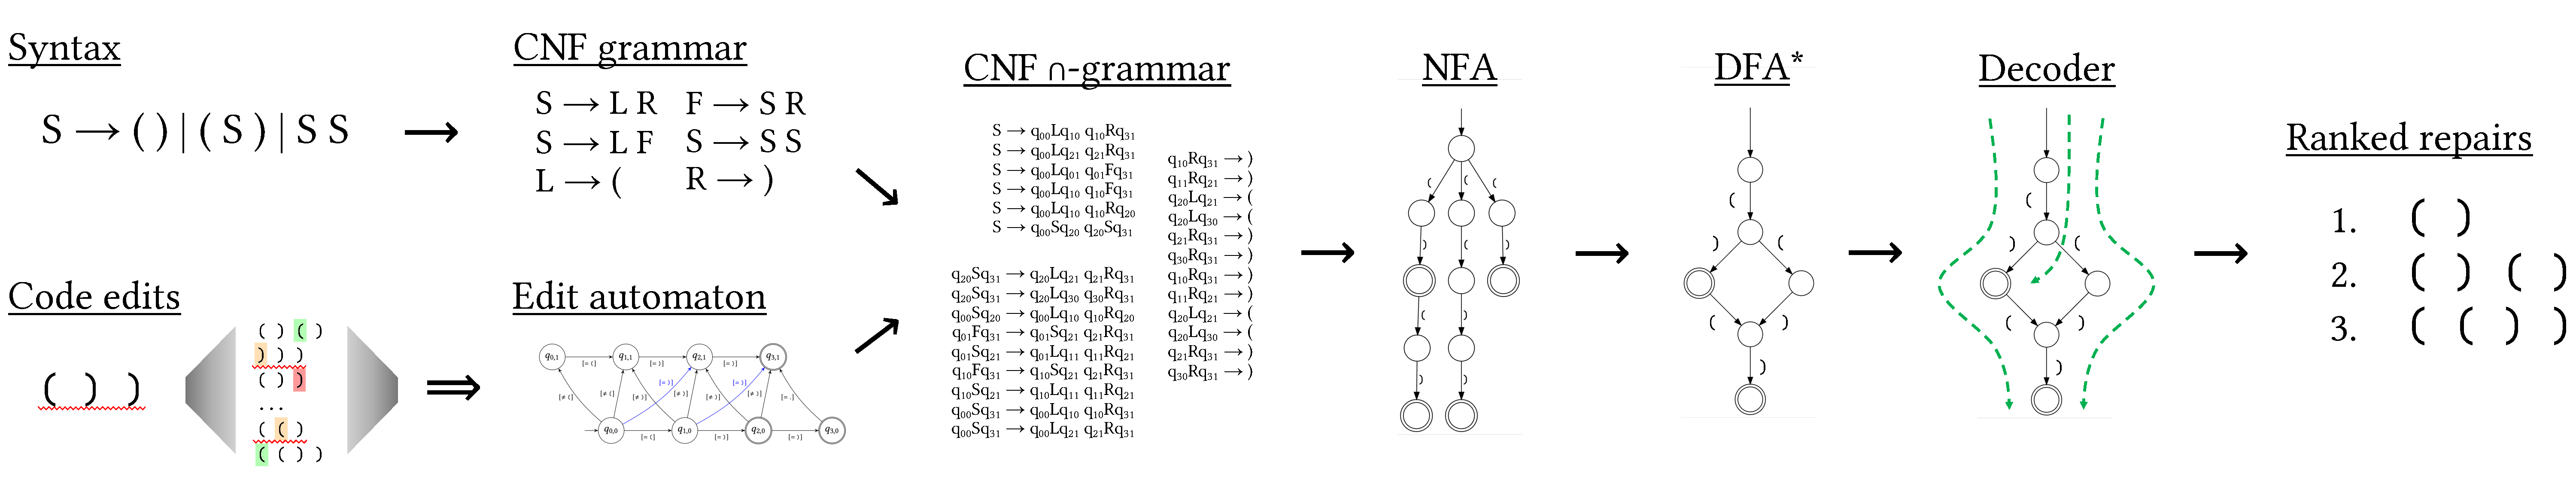
\includegraphics[width=\textwidth]{flow}\vspace{-1pt}
  \caption{Simplified dataflow. Given a grammar and broken code fragment, we create an automaton generating the language of small edits, then construct a regular expression representing the intersection of the two languages. This regular expression can be decoded to produce the final list of repairs.}\label{fig:arch_simp}
\end{figure}

To operationalize this technique, we design, develop and benchmark a new developer tool for syntax repair. This tool makes aggressive use of communication-free parallelism, making it readily executable by off-the-shelf GPU and SIMD co-processors. We provide a reference implementation of our tool on the WebGPU platform and show these computational resources, which typically sit idle during text editing, can be profitably used to accelerate real-time program repair.

Finally, we evaluate our approach on a dataset of human syntax errors and fixes fewer than five lexical edits and shorter than 120 tokens, large enough to fit a few lines of source code in realistic programming languages. Our work shows this technique is highly effective at predicting the true repair across a dataset of Python source code, on average 5x more accurately than previous state of the art methods at comparable latency and compute thresholds.

\section{Background}

Recall that a CFG, $\mathcal{G} = \langle \Sigma, V, P, S\rangle$, is a quadruple consisting of terminals $(\Sigma)$, nonterminals $(V)$, productions $\big(P\colon V \rightarrow (V \mid \Sigma)^+\big)$, and a start symbol, $(S)$. Every CFG is reducible to so-called \textit{Chomsky Normal Form}~\cite{chomsky1959certain}, $P'\colon V \rightarrow (V^2 \mid \Sigma)$, where every production is either (1) a binary production $w \rightarrow xz$, or (2) a unit production $w \rightarrow t$, where $w, x, z: V$ and $t: \Sigma$. For example:\vspace{-3pt}

\begin{table}[H]
  \begin{tabular}{llll}
    $G = \big\{\;S \rightarrow S\:S \mid (\:S\:) \mid (\:)\;\big\} \Longrightarrow G' = \big\{\;S\rightarrow Q\:R \mid S\:S \mid L\:R,$ & $R \rightarrow\:),$ & $L \rightarrow (,$ & $Q\rightarrow L\:S\;\big\}$
  \end{tabular}
\end{table}\vspace{-8pt}

Likewise, a finite state automaton (FSA) is a quintuple $\mathcal{A} = \langle Q, \Sigma, \delta, q_\alpha, F\rangle$, where $Q$ is a finite set of states, $\Sigma$ is a finite alphabet, $\delta \subseteq Q \times \Sigma \times Q$ is the transition function, $q_\alpha$ is the initial state, and $F \subseteq Q$ are the accepting states. These generally come in two varieties, deterministic and nondeterministic depending on whether or not $\delta$ maps each pair $\langle q, s \rangle$ to a unique $q'$.

There is an equivalent characterization of the regular languages via an inductively defined datatype, which is often more elegant than FSAs to work with. Consider the generalized regular expression (GRE) fragment containing concatenation, conjunction and disjunction:

\begin{definition}[Star-free GRE fragment]
  Let \( e \) be an expression defined by the grammar:
  \[
    e \rightarrow \varnothing \mid \varepsilon \mid \Sigma \mid e \cdot e \mid e \lor e \mid e \land e
  \]

where $\varepsilon$ is the empty symbol. Semantically, we interpret these expressions as denoting languages:\vspace{-0.8cm}

  \setlength{\columnseprule}{0pt}
  \setlength{\columnsep}{-3cm}
  \begin{multicols}{2}
    \begin{eqnarray*}
      \mathcal{L}(&\hspace{-0.35cm} \varnothing \hspace{-0.35cm}&) = \varnothing \\
      \mathcal{L}(&\hspace{-0.35cm} \varepsilon \hspace{-0.35cm}&) = \{\varepsilon\} \\
      \mathcal{L}(&\hspace{-0.35cm} a           \hspace{-0.35cm}&) = \{a\}
    \end{eqnarray*} \break\vspace{-0.45cm}
    \begin{eqnarray*}
      \mathcal{L}(&\hspace{-0.35cm} x\cdot z \hspace{-0.35cm}&) = \mathcal{L}(x) \circ \mathcal{L}(z)\text{\footnotemark}\\
      \mathcal{L}(&\hspace{-0.35cm} x\vee  z \hspace{-0.35cm}&) = \mathcal{L}(x) \cup  \mathcal{L}(z)\\
      \mathcal{L}(&\hspace{-0.35cm} x\land z \hspace{-0.35cm}&) = \mathcal{L}(x) \cap  \mathcal{L}(z)
    \end{eqnarray*}
  \end{multicols}
  \footnotetext{Where $\mathcal{L}(x)\circ\mathcal{L}(z)$ is defined as $\big\{a \cdot b \mid a \in \mathcal{L}(x) \land b \in \mathcal{L}(z) \big\}$.}
\end{definition}\vspace{-0.2cm}

\noindent Brzozowski~\cite{brzozowski1964derivatives} introduces an operator, $\partial$, which lets us quotient a language by some prefix,

\begin{definition}[Brzozowski, 1964]
  To compute the quotient \(\partial_a(L) = \{b \mid ab \in L\}\), we:

  \vspace{-0.8cm}
  \begin{multicols}{2}
    \begin{eqnarray*}
      \phantom{--}\partial_a(&\hspace{-0.35cm} \varnothing \hspace{-0.35cm}&) = \varnothing                                           \\
      \phantom{--}\partial_a(&\hspace{-0.35cm} \varepsilon \hspace{-0.35cm}&) = \varnothing                                           \\
      \phantom{--}\partial_a(&\hspace{-0.35cm} b           \hspace{-0.35cm}&) = \begin{cases}\varepsilon &\text{ if } a = b\\ \varnothing &\text{ if } a \neq b \end{cases}\\
      \phantom{--}\partial_a(&\hspace{-0.35cm} x\cdot z    \hspace{-0.35cm}&) = (\partial_a x)\cdot z \vee \delta(x)\cdot\partial_a z \\
      \phantom{--}\partial_a(&\hspace{-0.35cm} x\vee  z    \hspace{-0.35cm}&) =  \partial_a x \vee  \partial_a z                       \\
      \phantom{--}\partial_a(&\hspace{-0.35cm} x\land z    \hspace{-0.35cm}&) =  \partial_a x \land \partial_a z
    \end{eqnarray*} \break\vspace{-0.45cm}
    \begin{eqnarray*}
      \delta(&\hspace{-0.35cm} \varnothing \hspace{-0.35cm}&) = \varnothing                                      \\
      \delta(&\hspace{-0.35cm} \varepsilon \hspace{-0.35cm}&) = \varepsilon                                      \\
      \delta(&\hspace{-0.35cm} a           \hspace{-0.35cm}&) = \varnothing\phantom{\begin{cases}\varepsilon\\\varnothing\end{cases}}\\
      \delta(&\hspace{-0.35cm} x\cdot z    \hspace{-0.35cm}&) = \delta(x) \land \delta(z)                        \\
      \delta(&\hspace{-0.35cm} x\vee  z    \hspace{-0.35cm}&) = \delta(x) \vee  \delta(z)                        \\
      \delta(&\hspace{-0.35cm} x\land z    \hspace{-0.35cm}&) = \delta(x) \land \delta(z)
    \end{eqnarray*}
  \end{multicols}
\end{definition}

Primarily, this gadget was designed to handle membership queries, for which purpose it has received considerable attention~\cite{might2011parsing,adams2016complexity,stanford2021symbolic,varatalu2025re} in recent years:

\begin{theorem}[Recognition]
  For any regex \(e\) and \(\sigma: \Sigma^*\), \(\sigma \in \mathcal{L}(e) \Longleftrightarrow \varepsilon \in \mathcal{L}(\partial_\sigma e)\), where:

  \[
    \partial_\sigma (e): E \rightarrow E = \begin{cases}e &\text{ if } \sigma = \varepsilon\\\partial_b(\partial_a e) &\text{ if } \sigma = a \cdot b, a \in \Sigma, b \in \Sigma^* \end{cases}
  \]
\end{theorem}

Variations on this basic procedure can also be used for functional parsing and regular expression tasks. Less well known, perhaps, is that Brzozowski's derivative can also be used to decode witnesses. We will first focus on the nonempty disjunctive fragment, and define this process in two steps:

\begin{theorem}[Generation]\label{thm:generation}
  For any nonempty $(\varepsilon, \land)$-free regex, \(e\), to witness $\sigma \in \mathcal{L}(e)$:\\

  \hspace{1.6cm}$\texttt{follow}(e): E \rightarrow 2^\Sigma$ = \begin{cases}
   \{e\} &\text{ if } e \in \Sigma \\
   \texttt{follow}(x) &\text{ if } e = x \cdot z\\
   \texttt{follow}(x)\cup\texttt{follow}(z) &\text{ if } e = x \lor z
  \end{cases}\\\\

  \hspace{1.6cm}$\texttt{choose}(e): E \rightarrow \Sigma^+$ = \begin{cases}
   e &\text{ if } e \in \Sigma \\
   \big(s \stackrel{\$}{\gets} \texttt{follow}(e)\big)\cdot \texttt{choose}(\partial_s e) &\text{ if } e = x \cdot z\\
   \texttt{choose}\big(e' \stackrel{\$}{\gets} \{x, z\}\big) &\text{ if } e = x \lor z
  \end{cases}
\end{theorem}

Here, we use the $\stackrel{\$}{\gets}$ operator to denote probabilistic choice, however any deterministic choice function will also suffice to generate a witness. Now we are equipped to handle conjunction.

Recall that every regular language is also context-free a fortiori. So, given an $(\varepsilon, \land)$-free regular expression, we can construct an equivalent CFG with productions $P(e)$ as follows:

\begin{equation}
P(e): E \rightarrow \big(V \rightarrow (\Sigma \mid V \mid V^2)\big) = \begin{cases}
 \{ S_e \rightarrow e \} & \text{if } e \in \Sigma \\
 P(x) \cup P(z) \cup \{ S_e \rightarrow S_x S_z \} & \text{if } e = x \cdot z \\
 P(x) \cup P(z) \cup \{ S_e \rightarrow S_x, S_e \rightarrow S_z \} & \text{if } e = x \lor z \\
\end{cases}
\end{equation}\vspace{0.2cm}

\noindent where the CFG is $G(e) = \langle V, \Sigma, P(e), S_e\rangle$ with $V$ being all nonterminals in $P(e)$. Therefor, to intersect two regular languages, we can treat one of them as a CFL. Alternatively, we can take the intersection between some truly non-regular CFL (say, a programming language syntax) and a regular language.

\begin{theorem}[Bar-Hillel, 1961]
  For any CFG, $G = \langle V, \Sigma, P, S\rangle$, and nondeterministic finite automata (NFA), $A = \langle Q, \Sigma, \delta, q_\alpha, F\rangle$, there is a CFG, \(G_\cap=\langle V_\cap, \Sigma_\cap, P_\cap, S_\cap\rangle\) s.t. $\mathcal{L}(G_\cap) = \mathcal{L}(G)\cap\mathcal{L}(A)$.
\end{theorem}

\noindent Salomaa~\cite{salomaa1973formal} introduces a direct, but inefficient construction for the intersection grammar:

\begin{definition}[Salomaa, 1973]
  One could construct $G_\cap$ like so,

  \noindent\begin{prooftree}
      \hskip -0.5em
      \AxiomC{$q_\omega \in F\vphantom{\overset{a}{\rightarrow}}$}
      \RightLabel{$\mathcal{S}$}
      \UnaryInfC{$\big(S\rightarrow q_\alpha S q_\omega\big) \in P_\cap$}
      \DisplayProof
      \hskip 1em
      \AxiomC{$(w \rightarrow a) \in P$}
      \AxiomC{$(q\overset{a}{\rightarrow}r) \in \delta$}
      \RightLabel{$\uparrow$}
      \BinaryInfC{$\big(qwr\rightarrow a\big)\in P_\cap$}
      \DisplayProof
      \hskip 1em
      \AxiomC{$(w \rightarrow xz) \in P$}
      \AxiomC{$\vphantom{(}p,q,r \in Q\vphantom{\overset{a}{\rightarrow}}$}
      \RightLabel{$\Join$}
      \BinaryInfC{$\big(pwr\rightarrow (pxq)(qzr)\big) \in P_\cap$}
  \end{prooftree}
\end{definition}\vspace{0.2cm}

\noindent however most synthetic productions in $P_\cap$ will be non-generating or unreachable. This method will construct a synthetic production for state pairs which are not even connected by any path, which is clearly excessive. In \S~\ref{sec:method}, we will present a far more efficient construction for the special case when the intersection is finite. But first, let us return to the broader question of syntax repair.% We will instead proceed by considering a simpler problem, then construct a parse chart which efficiently computes the intersection.

\subsection{Informal statement}

Assume there exists a transducer from Unicode tokens to grammatical tokens, $\tau: \Sigma_U^* \rightarrow \Sigma_G^*$. In the compiler nomenclature $\tau$ is called a \textit{lexer} and would typically be regular under mild conditions. In this paper, we do not consider $\tau$ and strictly deal with languages over $\Sigma_G^*$, or simply $\Sigma^*$ for brevity.

%Thus, the full source language can be described as $\tau^{-1}\big(L(G)\big)$

%We designate a special token for tokens which are not recognized by the lexer, which are simply replaced by a hole.

Now suppose we have a syntax, $\ell \subset \Sigma^*$, containing every acceptable program. A syntax error is an unacceptable string, $\err\sigma \notin \ell$, that we wish to repair. We can model syntax repair as a language intersection between a context-free language (CFL) and a regular language. Henceforth, $\err\sigma$ will always and only be used to denote a syntactically invalid string whose target language is known.

\begin{wrapfigure}{r}{0.4\textwidth}
\vspace{-0.3cm}
\resizebox{0.42\textwidth}{!}{
  \def\secondcirclepath{(1.15,0) coordinate (e) circle (2cm)}
  \begin{tikzpicture}[
    dot/.style = {circle, inner sep=0pt, minimum size=1mm, fill,
    node contents={}}
  ]
    \def\firstcircle{(-2.1,0) coordinate (a) circle (2.4cm)}
    \def\firstcirclea{(-2.1,0) coordinate (b) circle (0.6cm)}
    \def\firstcircleb{(-2.1,0) coordinate (c) circle (1.2cm)}
    \def\firstcirclec{(-2.1,0) coordinate (d) circle (1.8cm)}
    \def\secondcircle{(1.2,0) coordinate (e) circle (1.5cm)}

    \begin{scope}
      \clip[decorate, decoration={snake, amplitude=0.6mm, segment length=5.01mm}] \secondcirclepath;
      \fill[black!35] \firstcircle;
    \end{scope}

    \draw \firstcircle node[dot,label=$\err{\sigma}$](z0);
    \draw [dashed] \firstcirclea;
    \draw [dashed] \firstcircleb;
    \draw [dashed] \firstcirclec;
    \draw[-stealth] (-2.1,0) -- (-1.5, 0) node[midway,below]{$d_1$};
    \draw[-stealth] (-1.5,0) -- (-0.9, 0) node[midway,below]{$d_2$};
    \draw[-stealth] (-0.9,0) -- (-0.3, 0) node[midway,below]{$d_3$};
    \draw[-stealth] (-0.3,0) -- (0.3, 0) node[midway,above]{$\tilde{\sigma}$};
    \draw[-stealth] (-0.3,0) -- (0.3, 0) node[midway,below]{$d_4$};

    \draw[decorate, decoration={snake, amplitude=0.6mm, segment length=5.01mm}] \secondcirclepath;
    \node [above] at (current bounding box.north -| a) {$\mathcal{L}\bigl(L(\err\sigma, d^* + 1)\bigr)$};
    \node [above,yshift=2.1cm] at (e) {$\mathcal{L}(G)$};
    \node [above,yshift=1.8cm, xshift=-1.4cm] at (e) {$\ell_\cap$};
  \end{tikzpicture}
}
\vspace{-0.3cm}
\caption{CFL intersection with the local edit region around a given broken code snippet.}
\vspace{-0.2cm}
\end{wrapfigure}

Given a lexical representation of a broken computer program $\err\sigma$ and a grammar $G$, our goal is to find every valid string $\sigma$ consistent with the grammar $G$ and within a certain edit distance, $d$. Consider the language of nearby strings: if intersected with the language of grammatically valid programs, $\mathcal{L}(G)$, the result ($\ell_\cap$) will contain every possible repair within the given edit distance, a subset of which will be natural or statistically probable. If we can locate these repairs then we can map them back into Unicode, adding placeholders for fresh names, numbers, and string literals, then finally apply an off-the-shelf code formatter to display them. Both the preprocessing and the cosmetic postprocessing steps are tangential to this work, in which we confine ourselves to a lexical alphabet.

\subsection{Formal statement}\label{sec:problem}

Let us now restate our informal description of the syntax repair problem in more formal terms.

\begin{definition}[Bounded Levenshtein-CFL reachability]\label{def:bcflr}
Given a CFL, $\ell$, and an invalid string, $\err{\sigma}: \bar\ell$, find every valid string reachable within $d$ edits of $\err{\sigma}$, i.e., letting $\Delta$ be the Levenshtein metric and $\mathcal{L}\big(L(\err\sigma, d)\big) = \{\sigma' \mid \Delta(\err{\sigma}, \sigma') \leq d\}$ be the Levenshtein $d$-ball, we seek to find $\ell_\cap = \mathcal{L}\big(L(\err\sigma, d)\big) \cap \ell$.
\end{definition}

%  To solve this problem, it is convenient to first consider intersections with a finite-length string with holes, then turn our attention back to BCFLR.
%

As the admissible set $\ell_\cap$ is typically under-constrained, we want a procedure which surfaces natural and valid repairs over unnatural but valid repairs:

\begin{definition}[Ranked repair]\label{def:ranked-repair}
Given a finite language $\ell_\cap = \mathcal{L}\big(L(\err\sigma, d)\big) \cap \ell$ and a probabilistic language model $\text{P}_\theta: \Sigma^* \rightarrow [0, 1] \subset \mathbb{R}$, find the top-$k$ maximum probability repairs. That is,
\begin{equation}
R(\ell_\cap, P_\theta): 2^{\Sigma^*} \times (\Sigma^* \rightarrow \mathbb{R}) \rightarrow (\Sigma^*)^{\leq k} = \argmax_{\bm{\sigma} \subseteq \ell_\cap, |\bm{\sigma}| \leq k} \sum_{\sigma \in \bm{\sigma}}\text{P}_\theta(\sigma)
\end{equation}
% On average, across all $G, \sigma$ $\hat{R}$ should approximate $R$.
%    We want a procedure $\hat{R}$, minimizing $\mathbb{E}_{G, \sigma}\big[D_{\text{KL}}(\hat{R} \parallel R)\big]$ and wallclock runtime.
\end{definition}

A popular approach to ranked repair involves learning a distribution over strings, however this is highly sample-inefficient and generalizes poorly to new languages. Approximating a distribution over $\Sigma^*$ forces the model to jointly learn syntax and stylometry. Furthermore, even with an extremely efficient approximate sampler for $\sigma \sim \ell_\cap$, due to the size of the languages involved, it would be intractable to sample either $\ell$ or $\mathcal{L}\big(L(\err\sigma, d)\big)$, reject duplicates, then reject unreachable or invalid edits, and completely out of the question to sample $\sigma \sim \Sigma^*$ as do many neural language models.

As we will demonstrate, the ranked repair problem can be factorized into two steps: first exact representation, then decoding. Instead of working with strings, we will explicitly construct a grammar which soundly and completely generates the set $\ell \cap \mathcal{L}\big(L(\err\sigma, d)\big)$, then retrieve repairs from its language. By ensuring retrieval is sufficiently precise and exhaustive, maximizing probability over the retrieved set can be achieved with a much simpler, syntax-oblivious language model.

%Assuming we have a grammar that recognizes the Levenshtein-CFL intersection, the question then becomes how to maximize the number of unique valid sentences in a given number of samples. Top-down incremental sampling with replacement eventually converges to the language, but does so superlinearly~\cite{flajolet1992birthday}. Due to practical considerations including latency, we require the sampler to converge linearly, ensuring with much higher probability that natural repairs are retrieved in a timely manner. This motivates the need for a specialized generating function. More precisely,
%
%\begin{definition}[Linear convergence]\label{def:linear-convergence}
%Given a finite CFL, $\ell$, we want a randomized generating function, $\bm{\varphi}: \mathbb{N}_{\leq|\ell|} \rightarrow 2^\ell$, whose rate of convergence is linear in expectation, i.e., $\mathbb{E}_{i \in [1, n]}|\bm{\varphi}(i)| \propto n$.
%\end{definition}
%
%\noindent This will ensure that if $|\ell_\cap|$ is sufficiently small and enough samples are drawn, $\bm\varphi$ is sure to include a representative subset, and additionally, will terminate after exhausting all valid repairs.
%
%To satisfy Def.~\ref{def:linear-convergence}, we can construct a bijection from syntax trees to integers (\S~\ref{sec:ptree}), sample integers uniformly without replacement, then decode them as trees. This will produce a set of unique trees, and each tree, assuming grammatical unambiguity, will correspond to a unique sentence in the language.  Finally, sentences can be scored and ranked by likelihood under a language model.
%
%Otherwise, if the grammar, $G_\ell$, is ambiguous, it can be translated into a DFA, then decoded (\S~\ref{sec:decoding}) using an autoregressive language model or any suitably fast scoring function of the implementer's choice. In our case, we use a low-order Markov model for its inference speed, data efficiency, and simplicity. So long as the decoder samples $\ell$ without replacement, it will satisfy Def.~\ref{def:linear-convergence}.

%  Finally, once we have a set of small and valid repairs, the problem of ranked repair reduces to sorting retrieved samples by likelihood, which can be approximated using an autoregressive language model or any suitable scoring function of the implementer's choice.

\clearpage\section{Method}\label{sec:method}

The key to solving this problem is to treat finite language intersections as matrix exponentiation. We will show a certain correspondence between CFL-REG intersections and a semiring algebra that allows us to quickly decide and witness intersection nonemptiness for finite languages.

\begin{theorem}%[Considine, 2025]
  For every CFG, G, and every acyclic NFA (ANFA), $A = \langle Q, \Sigma, \delta, q_\alpha: Q, F \subseteq Q\rangle$, there exists a decision procedure $\Psi: \text{CFG} \rightarrow \text{ANFA} \rightarrow \mathbb{B}$ such that $\Psi(G, A) \models [\mathcal{L}(G)\cap\mathcal{L}(A) \neq \varnothing]$ which requires $\mathcal{O}\big(\log^c |Q||V|\big)$ time using $\mathcal{O}\big((|Q||V|)^k\big)$ parallel processors for some $c, k < \infty$.
\end{theorem}

\begin{proof}[Proof]
  To prove nonemptiness, we must show there exists a path $q_\alpha \rightsquigarrow q_\omega$ in $A$ such that $q_\omega: F$ where $q_\alpha \rightsquigarrow q_\omega \vdash S$. At least one of two cases must hold for $w \in V$ to parse a given $p \rightsquigarrow r$ pair:

  \begin{enumerate}
    \item $p$ steps directly to $r$ in which case it suffices to check $\exists a.\big((p \overset{a}{\rightarrow} r)\in \delta \land (w \rightarrow a) \in P\big)$, or,
    \item there is some midpoint $q \in Q$, $p \rightsquigarrow q \rightsquigarrow r$ such that $\exists x, z.\big((w \rightarrow xz) \in P\land\overbrace{\underbrace{p \rightsquigarrow q}_x, \underbrace{q \rightsquigarrow r}_z}^w\big)$.
  \end{enumerate}

  \noindent This decomposition immediately suggests a dynamic programming solution. Let M be a matrix of type $E^{|Q|\times|Q|\times|V|}$  indexed by $Q$. Since we assumed $\delta$ is acyclic, there exists a topological sort of $\delta$ imposing a total order on $Q$ such that $M$ is strictly upper triangular (SUT). Initiate it thusly:

  \begin{align}
    M_0[r, c, w] = \bigvee_{a\::\:\Sigma} \big\{a \mid (w \rightarrow a) \in P \land (q_r \overset{a}{\rightarrow} q_c)\in \delta\big\}
  \end{align}

  Now, our goal will be to find $M=M^2$ such that $\big[M_0[r, c, w] \neq \varnothing\big] \implies \big[M[r, c, w] \neq \varnothing\big]$ under a certain near-semiring. The algebraic operations $\oplus, \otimes: E^{2|V|} \rightarrow E^{|V|}$ we will define elementwise:

  \begin{equation}
    [\ell \oplus r]_w  = [\ell_w \lor r_w]\hspace{0.5cm}\text{and}\hspace{0.5cm}
    [\ell \otimes r]_w = \bigvee_{\mathclap{x, z\:\in\:V}}\big\{\ell_x \cdot r_z \mid (w \rightarrow xz) \in P\big\}
  \end{equation}

  \noindent By slight abuse of notation,\footnote{Customarily, there is a $\frac{1}{k!}$ factor to suppress exploding entries, but alas this domain has no multiplicative inverse.} we will redefine the matrix exponential over this domain as:

  \begin{align}
    \exp(M) &= \sum_{i = 0}^\infty M_0^i = \sum_{i = 0}^{\mathclap{|Q||V|}} M_0^i \text { (since $M$ is SUT.)}
  \end{align}

  \noindent While $|Q||V|$ is an upper-bound and $\exp(M)$ may converge sooner, incremental evaluation grows expensive even with unbounded parallelism. Instead, we will employ exponentiation-by-squaring:

  \begin{align}
    T(2n) \;=\; \begin{cases}
       M_0, & \text{if } n = 1,\\
       T(n) + T(n)^2 & \text{otherwise}.
    \end{cases}
  \end{align}

  \noindent Therefor, the complexity can be reduced to at most $\lceil\log_2 |Q||V|\rceil$ sequential steps in the limit. Finally, we will union all the languages of every state pair deriving $S$ into a new nonterminal, $S_\cap$.

  \begin{align}
    S_\cap = \bigvee_{\mathclap{\:q_\omega \in F}}\exp(M)[q_\alpha, q_\omega, S] \text{ and } \Psi = [S_\cap \neq \varnothing]
  \end{align}

  \noindent Note we can check $\Psi$ before each recurrence of $T$ and escape immediately thereafter in case of nonemptiness. Should that occur, one may simply $\texttt{choose}(S_\cap)$ to decode a witness (see Thm.~\ref{thm:generation}). In either case, the algorithm provably terminates in $\mathcal{O}\big(\log^c |Q||V|\big)$ parallel time for finite $c$.
\end{proof}\clearpage

\section{Examples}

In this section, we will consider three examples of intersections with finite languages. First, parsing can be viewed as a special case of intersection with a singleton language. Second, we will introduce completion as intersection admitting terminal wildcards in fixed locations. Thirdly, we consider syntax repair, where we will intersect a language representing all possible edit paths within a certain distance to determine the location(s) and fill them with appropriate terminal(s).

\subsection{Recognition as intersection}

In the case of ordinary CFL recognition, the automaton accepts just a single word:

\begin{figure}[H]
\resizebox{0.5\textwidth}{!}{
  \begin{tikzpicture}[>=stealth', node distance=2.5cm, initial text=$ $]
    \node[state, initial]         (00) {$q_{0,0}$};
    \node[state, right of=00]     (10) {$q_{1,0}$};
    \node[state, right of=10, draw=none]     (20) {$\ldots$};
    \node[state, accepting, right of=20] (30) {$q_{n,0}$};

    \draw [->] (00) edge[below] node{$\sigma_1$} (10);
    \draw [->] (10) edge[below] node{$\sigma_2$} (20);
    \draw [->] (20) edge[below] node{$\sigma_n$} (30);
  \end{tikzpicture}
}
\end{figure}

Given a CFG, $G' : \mathcal{G}$ in Chomsky Normal Form (CNF), we can construct a recognizer for strings $\sigma: \Sigma^n$ as follows. Let $2^V$ be our domain, $0$ be $\varnothing$, $\oplus$ be $\cup$, and $\otimes$ be defined as:\vspace{-10pt}

\begin{align}
  X \otimes Z = \big\{\;w \mid \langle x, z\rangle \in X \times Z, (w\rightarrow xz) \in P\;\big\}
\end{align}

\noindent If we define $\hat\sigma_r = \{w \mid (w \rightarrow \sigma_r) \in P\}$, then construct a matrix with nonterminals on the superdiagonal representing each token, $M_0[r+1=c](G', \sigma) = \;\hat\sigma_r$, the fixpoint $M_{i+1} = M_i + M_i^2$ is uniquely determined by the superdiagonal entries. Omitting the exponentiation-by-squaring detail, the ordinary fixedpoint iteration simply fills successive diagonals:\vspace{-10pt}

\begin{align*}
  M_0=
  \begin{pNiceMatrix}[nullify-dots,xdots/line-style=loosely dotted]
    \varnothing & \hat\sigma_1 & \varnothing & \Cdots & \varnothing  \\
    \Vdots      & \Ddots       & \Ddots      & \Ddots & \Vdots       \\
                &              &             &        & \varnothing  \\
                &              &             &        & \hat\sigma_n \\
    \varnothing & \Cdots       &             &        & \varnothing
  \end{pNiceMatrix} & \Rightarrow
  \begin{pNiceMatrix}[nullify-dots,xdots/line-style=loosely dotted]
    \varnothing & \hat\sigma_1 & \Lambda     & \Cdots & \varnothing  \\
    \Vdots      & \Ddots       & \Ddots      & \Ddots & \Vdots       \\
                &              &             &        & \Lambda      \\
                &              &             &        & \hat\sigma_n \\
    \varnothing & \Cdots       &             &        & \varnothing
  \end{pNiceMatrix} & \Rightarrow \ldots \Rightarrow M_\infty =
  \begin{pNiceMatrix}[nullify-dots,xdots/line-style=loosely dotted]
    \varnothing & \hat\sigma_1 & \Lambda     & \Cdots & \Lambda^*_\sigma \\
    \Vdots      & \Ddots       & \Ddots      & \Ddots & \Vdots           \\
                &              &             &        & \Lambda          \\
                &              &             &        & \hat\sigma_n     \\
    \varnothing & \Cdots       &             &        & \varnothing
  \end{pNiceMatrix}
\end{align*}

Once the fixpoint $M_\infty$ is attained, the proposition $[S \in \Lambda^*_\sigma]$~\footnote{Hereinafter, we use Iverson brackets to denote the indicator function of a predicate with free variables, i.e., $[P] \Leftrightarrow \mathds{1}(P)$.} decides language membership, i.e., $[\sigma \in \mathcal{L}(G)]$. So far, this procedure is essentially the textbook CYK algorithm in a linear algebraic notation~\cite{goodman1999semiring} and a well-established technique in the parsing literature~\cite{Grune2008}.

\subsection{Completion as intersection}

We may also consider a problem of intermediate difficulty, wherein we are given a string template admitting edits at fixed locations, which can be filled by any terminal. When intersected with a CFL, this specifies a finite language whose contents are the set of all words consistent with the template. This problem we call \textit{completion}. Formally,

\begin{definition}[Completion]
  Let $\underline\Sigma = \Sigma \cup \{\_\}$, where $\_$ denotes a hole. We denote $\sqsubseteq: \Sigma^n \times \underline\Sigma^n$ as the relation $\{\langle\sigma', \sigma\rangle \mid \sigma_i \in \Sigma \implies \sigma_i' = \sigma_i\}$ and the set of all inhabitants $\{\sigma': \Sigma^+ \mid \sigma' \sqsubseteq \sigma\}$ as $\text{H}(\sigma)$. Given a \textit{porous string}, $\sigma: \underline\Sigma^*$ we seek all syntactically valid inhabitants, i.e., $A(\sigma)=\text{H}(\sigma)\cap\ell$.
\end{definition}

Here, the FSA takes a similar shape but can have multiple arcs between adjacent states, e.g.:

\begin{figure}[H]
  \resizebox{0.5\textwidth}{!}{
    \begin{tikzpicture}[>=stealth', node distance=2.5cm, initial text=$ $]
      \node[state, initial]                (00) {$q_{0,0}$};
      \node[state, right of=00]            (10) {$q_{1,0}$};
      \node[state, right of=10]            (20) {$q_{2,0}$};
      \node[state, accepting, right of=20] (30) {$q_{3,0}$};

      \draw [->] (00) edge[below]             node{$\sigma_1$} (10);
      \draw [->] (10) edge[below]             node{$\ldots$}   (20);
      \draw [->] (10) edge[below, bend left]  node{$\Sigma_1$} (20);
      \draw [->] (10) edge[below, bend right] node{$\Sigma_n$} (20);
      \draw [->] (20) edge[below]             node{$\ldots$}   (30);
      \draw [->] (20) edge[below, bend left]  node{$\Sigma_1$} (30);
      \draw [->] (20) edge[below, bend right] node{$\Sigma_n$} (30);
    \end{tikzpicture}
  }
\end{figure}

\noindent This corresponds to a template with two holes, $\sigma = 1$ \_ \_. Suppose the context-free grammar is $G=\{S\rightarrow N O N, O \rightarrow + \mid \times, N \rightarrow 0 \mid 1\}$. This grammar will first be rewritten into CNF as $G'= \{S \rightarrow N L, N \rightarrow 0 \mid 1, O \rightarrow \times \mid +, L \rightarrow O N\}$. Using the powerset algebra we just defined, the matrix fixpoint $M' = M + M^2$ can be computed as follows, shown in the leftmost column below:\vspace{0.3cm}

\begin{small}
{\renewcommand{\arraystretch}{1.2}
\noindent\phantom{...}\begin{tabular}{|c|c|c|c|}
  \hline
  & $2^V$ & $\mathbb{Z}_2^{|V|}$ & $\mathbb{Z}_2^{|V|}\rightarrow\mathbb{Z}_2^{|V|}$\\\hline
  $M_0$ & \begin{pmatrix}
            \phantom{V} & \tiny{\{N\}} &              &              \\
                        &              & \{N,O\}      &              \\
                        &              &              & \{N,O\}      \\
                        &              &              &
  \end{pmatrix} & \begin{pmatrix}
            \phantom{V} & \overset{L}{\ws}\overset{N}{\bs}\overset{O}{\ws}\overset{S}{\ws} &              &              \\
                        &              & \ws\bs\bs\ws &              \\
                        &              &              & \ws\bs\bs\ws \\
                        &              &              &
  \end{pmatrix} & \begin{pmatrix}
            \phantom{V} & V_{0, 1}     &              &              \\
                        &              & V_{1, 2}     &              \\
                        &              &              & V_{2, 3}     \\
                        &              &              &
  \end{pmatrix} \\\hline
  $M_1$ & \begin{pmatrix}
            \phantom{V} & \tiny{\{N\}} & \varnothing  &              \\
                        &              & \{N,O\}      & \{L\}        \\
                        &              &              & \{N,O\}      \\
                        &              &              &
  \end{pmatrix} & \begin{pmatrix}
            \phantom{V} & \ws\bs\ws\ws & \ws\ws\ws\ws &              \\
                        &              & \ws\bs\bs\ws & \bs\ws\ws\ws \\
                        &              &              & \ws\bs\bs\ws \\
                        &              &              &
  \end{pmatrix} & \begin{pmatrix}
            \phantom{V} & V_{0, 1}     & V_{0, 2}     &              \\
                        &              & V_{1, 2}     & V_{1, 3}     \\
                        &              &              & V_{2, 3}     \\
                        &              &              &
  \end{pmatrix} \\\hline
  \begin{tabular}{@{}c@{}}$M_2$\\$=$\\$M_\infty$\end{tabular} & \begin{pmatrix}
            \phantom{V} & \tiny{\{N\}} & \varnothing  & \{S\}        \\
                        &              & \{N,O\}      & \{L\}        \\
                        &              &              & \{N,O\}      \\
                        &              &              &
  \end{pmatrix} & \begin{pmatrix}
            \phantom{V} & \ws\bs\ws\ws & \ws\ws\ws\ws & \ws\ws\ws\bs \\
                        &              & \ws\bs\bs\ws & \bs\ws\ws\ws \\
                        &              &              & \ws\bs\bs\ws \\
                        &              &              &
  \end{pmatrix} & \begin{pmatrix}
            \phantom{V} & V_{0, 1}     & V_{0, 2}     & V_{0, 3}     \\
                        &              & V_{1, 2}     & V_{1, 3}     \\
                        &              &              & V_{2, 3}     \\
                        &              &              &
  \end{pmatrix} \\\hline
\end{tabular}\\
}
\end{small}

\vspace{8pt}The same procedure can be translated, without loss of generality, into the bit domain ($\mathbb{Z}_2^{|V|}$) using a lexicographic nonterminal ordering, however $M_\infty$ in both $2^V$ and $\mathbb{Z}_2^{|V|}$ represents a decision procedure, i.e., $\big[S\in M_\infty[0, 3]\big]\Leftrightarrow \big[M_\infty[0, 3, 3]=\bs\big] \Leftrightarrow \big[A(\sigma) \neq \varnothing\big]$. Since $M_\infty[0, 3] = \{S\}$, we know there is at least one $\sigma' \in A(\sigma)$, but neither $M_\infty$ in $2^V$ or $\mathbb{Z}_2^V$ lets us recover a witness.

%$\{\text{xor}, \land, \top\}$ is a functionally complete set is equivalent to $\mathbb{Z}_2$ $\top := 1, \land := \times, \text{xor} := +$. We can define $=$ as $(a = b) \Leftrightarrow (a \text{ xor } b) \text{ xor } \top \Leftrightarrow (a + b) + \top$.

To witness $\sigma' \in A(\sigma)$, we can translate the matrix exponential to the GRE domain. We first define $X \boxtimes Z = [X_2 \cdot Z_1, \varnothing, \varnothing, X_1 \cdot Z_0]$ and $X \boxplus Z = [X_i \lor Z_i]_{i \in [0, |V|)}$, mirroring $\oplus, \otimes$ from the powerset domain. Since the unit nonterminals $O, N$ can only occur on the superdiagonal, they may be safely ignored by $\boxtimes$. To solve for $M_\infty$, we proceed by first computing $E_{0, 2}, E_{1, 3}$:\vspace{-8pt}

\begin{small}
\begin{align*}
  E_{0, 2} &= E_{0, j} \cdot E_{j, 2} = E_{0, 1} \boxtimes E_{1, 2}                         &  E_{1, 3} &= E_{1, j} \cdot E_{j, 3} = E_{1, 2} \boxtimes E_{2, 3}\\
  &= [L \in E_{0, 2}, \varnothing, \varnothing, S \in E_{0, 2}]                                           &  &= [L \in E_{1, 3}, \varnothing, \varnothing, S \in E_{1, 3}]\\
  &= [O \in E_{0, 1} \cdot N \in E_{1, 2}, \varnothing, \varnothing, N \in E_{0, 1} \cdot L \in E_{1, 2}] &  &= [O \in E_{1, 2} \cdot N \in E_{2, 3}, \varnothing, \varnothing, N \in E_{1, 2} \cdot L \in E_{2, 3}]\\
  &= [E_{0, 1, 2} \cdot E_{1, 2, 1}, \varnothing, \varnothing, E_{0, 1, 1} \cdot E_{1, 2, 0}]             &  &= [E_{1, 2, 2} \cdot E_{2, 3, 1}, \varnothing, \varnothing, E_{1, 2, 1} \cdot E_{2, 3, 0}]
\end{align*}
\end{small}\vspace{-8pt}

\noindent Now we solve for the corner entry $E_{0, 3}$ by dotting the first row and last column, which yields:\vspace{-8pt}

\begin{align*}
  E_{0, 3} &= E_{0, j} \cdot E_{j, 3} = (E_{0, 1} \boxtimes E_{1, 3}) \boxplus (E_{0, 2} \boxtimes E_{2, 3})\\
%  &= [E_{0, 1, 2} \cdot E_{1, 3, 1}, \varnothing, \varnothing, E_{0, 1, 1} \cdot E_{1, 3, 0}] + [E_{0, 2, 2} \cdot E_{2, 3, 1}, \varnothing, \varnothing, E_{0, 2, 1} \cdot E_{2, 3, 0}]\\
  &= [E_{0, 1, 2} \cdot E_{1, 3, 1} \lor E_{0, 2, 2} \cdot E_{2, 3, 1}, \varnothing, \varnothing, E_{0, 1, 1} \cdot E_{1, 3, 0} \lor E_{0, 2, 1} \cdot E_{2, 3, 0}]
\end{align*}

\noindent Since we only care about $E_{0, 3, 3} \Leftrightarrow [S \in E_{0, 3}]$, we can ignore the first three entries and solve for:\vspace{-8pt}

\begin{align*}
  E_{0, 3, 3} &= E_{0, 1, 1} \cdot E_{1, 3, 0} \lor E_{0, 2, 1} \cdot E_{2, 3, 0}\\
  &= E_{0, 1, 1} \cdot (E_{1, 2, 2} \cdot E_{2, 3, 1}) \lor E_{0, 2, 1} \cdot \varnothing\\
  &= E_{0, 1, 1} \cdot E_{1, 2, 2} \cdot E_{2, 3, 1} \big(= [N \in E_{0, 1}] \cdot [O \in E_{1, 2}] \cdot [N \in E_{2, 3}]\big)\\
  &= 1 \cdot \{+, \times\} \cdot \{0, 1\}
\end{align*}

\noindent Finally, to recover a witness, we can simply $\texttt{choose}\big(1 \cdot \{+, \times\} \cdot \{0, 1\}\big)$.

%Now we know that $\sigma =$ 1 \underline{O} \underline{N} is a valid solution, and we can take the product $\{1\}\times \hat\sigma_2^{-1}(O) \times \hat\sigma_3^{-1}(N)$ to recover the inhabitants, yielding $A=\{1+0, 1+1, 1\times 0, 1\times 1\}$. In this case, since $G$ is unambiguous, there is only one parse tree satisfying $V_{0, |\sigma|, 3}$.%, but in general, there can be multiple valid parse trees.

\subsection{Repair as intersection}\label{sec:repair_ex}

Now, we are ready to consider the general case of syntax repair, in which case the edit locations are not localized but can occur anywhere inside the snippet. In this case, we construct a lattice of all possible edit paths up to a fixed distance. This structure is called a Levenshtein automaton.

\begin{wrapfigure}{r}{0.5\textwidth}
  \vspace{-0.3cm}
  \begin{center}
      \resizebox{0.5\textwidth}{!}{
  \begin{tikzpicture}[
%->, % makes the edges directed
  >=stealth',
  node distance=2.5cm, % specifies the minimum distance between two nodes. Change if necessary.
%  every state/.style={thick, fill=gray!10}, % sets the properties for each ’state’ node
  initial text=$ $, % sets the text that appears on the start arrow
  ]
  \node[state, initial]                (00) {$q_{0,0}$};
  \node[state, right of=00]            (10) {$q_{1,0}$};
  \node[accepting, state, right of=10] (20) {$q_{2,0}$};
  \node[accepting, state, right of=20] (30) {$q_{3,0}$};
  \node[accepting, state, right of=30] (40) {$q_{4,0}$};
  \node[accepting, state, right of=40] (50) {$q_{5,0}$};

  \node[state, above of=00, shift={(-2cm,0cm)}] (01) {$q_{0,1}$};
  \node[state, right of=01]                          (11) {$q_{1,1}$};
  \node[state, right of=11]                          (21) {$q_{2,1}$};
  \node[accepting, state, right of=21]               (31) {$q_{3,1}$};
  \node[accepting, state, right of=31]               (41) {$q_{4,1}$};
  \node[accepting, state, right of=41]               (51) {$q_{5,1}$};

\node[state, above of=01, shift={(-2cm,0cm)}] (0j) {$q_{0,2}$};
\node[state, right of=0j]                          (1j) {$q_{1,2}$};
\node[state, right of=1j]                          (2j) {$q_{2,2}$};
\node[state, right of=2j]                          (3j) {$q_{3,2}$};
\node[accepting, state, right of=3j]               (4j) {$q_{4,2}$};
\node[accepting, state, right of=4j]               (5j) {$q_{5,2}$};

\node[state, above of=0j, shift={(-2cm,0cm)}] (0k) {$q_{0,3}$};
\node[state, right of=0k]                         (1k) {$q_{1,3}$};
\node[state, right of=1k]                         (2k) {$q_{2,3}$};
\node[state, right of=2k]                         (3k) {$q_{3,3}$};
\node[state, right of=3k]                         (4k) {$q_{4,3}$};
\node[accepting, state, right of=4k]              (5k) {$q_{5,3}$};

\draw [->] (00) edge[below] node{$\sigma_1$} (10);
\draw [->] (10) edge[below] node{$\sigma_2$} (20);
\draw [->] (20) edge[below] node{$\sigma_3$} (30);
\draw [->] (30) edge[below] node{$\sigma_4$} (40);
\draw [->] (40) edge[below] node{$\sigma_5$} (50);

\draw [->] (01) edge[below] node{$\sigma_1$} (11);
\draw [->] (11) edge[below] node[shift={(-0.2cm,0cm)}]{$\sigma_2$} (21);
\draw [->] (21) edge[below] node[shift={(-0.2cm,0cm)}]{$\sigma_3$} (31);
\draw [->] (31) edge[below] node[shift={(-0.2cm,0cm)}]{$\sigma_4$} (41);
\draw [->] (41) edge[below] node{$\sigma_5$} (51);

\draw [->] (0j) edge[below] node{$\sigma_1$} (1j);
\draw [->] (1j) edge[below] node{$\sigma_2$} (2j);
\draw [->] (2j) edge[below] node{$\sigma_3$} (3j);
\draw [->] (3j) edge[below] node{$\sigma_4$} (4j);
\draw [->] (4j) edge[below] node{$\sigma_5$} (5j);

\draw [->] (0k) edge[below] node{$\sigma_1$} (1k);
\draw [->] (1k) edge[below] node{$\sigma_2$} (2k);
\draw [->] (2k) edge[below] node{$\sigma_3$} (3k);
\draw [->] (3k) edge[below] node{$\sigma_4$} (4k);
\draw [->] (4k) edge[below] node{$\sigma_5$} (5k);

\draw [->] (00) edge[left] node{$\phantom{\cdot}$} (11);
\draw [->] (10) edge[left] node{$\phantom{\cdot}$} (21);
\draw [->] (20) edge[left] node{$\phantom{\cdot}$} (31);
\draw [->] (30) edge[left] node{$\phantom{\cdot}$} (41);
\draw [->] (40) edge[left] node{$\phantom{\cdot}$} (51);

% Super-knight arcs
\draw [->, red] (00) edge[bend right=8] node[east, shift={(-0.2cm,-0.7cm)}]{$\color{red}\sigma_3$}         (3j);
\draw [->, red] (10) edge[bend right=8] node[east, shift={(-0.2cm,-0.7cm)}]{$\color{red}\sigma_4$}         (4j);
\draw [->, red] (20) edge[bend right=8] node[east, shift={(-0.2cm,-0.7cm)}]{$\color{red}\sigma_5$}         (5j);

\draw [->, red] (01) edge[bend left=8] node[east, shift={(-0.2cm,-0.7cm)}]{$\color{red}\sigma_3$}         (3k);
\draw [->, red] (11) edge[bend left=8] node[east, shift={(-0.2cm,-0.7cm)}]{$\color{red}\sigma_4$}         (4k);
\draw [->, red] (21) edge[bend left=8] node[east, shift={(-0.2cm,-0.7cm)}]{$\color{red}\sigma_5$}         (5k);

\draw [->, violet] (00) edge node[east, shift={(-0.1cm,-0.8cm)}]{$\color{violet}\sigma_4$}  (4k);
\draw [->, violet] (10) edge node[east, shift={(-0.1cm,-0.8cm)}]{$\color{violet}\sigma_5$}  (5k);

\draw [->] (01) edge[left] node{$\phantom{\cdot}$} (1j);
\draw [->] (11) edge[left] node{$\phantom{\cdot}$} (2j);
\draw [->] (21) edge[left] node{$\phantom{\cdot}$} (3j);
\draw [->] (31) edge[left] node{$\phantom{\cdot}$} (4j);
\draw [->] (41) edge[left] node{$\phantom{\cdot}$} (5j);

\draw [->] (0j) edge[left] node{$\phantom{\cdot}$} (1k);
\draw [->] (1j) edge[left] node{$\phantom{\cdot}$} (2k);
\draw [->] (2j) edge[left] node{$\phantom{\cdot}$} (3k);
\draw [->] (3j) edge[left] node{$\phantom{\cdot}$} (4k);
\draw [->] (4j) edge[left] node{$\phantom{\cdot}$} (5k);

\draw [->] (00) edge[bend left=10, left] node{$\phantom{\cdot}$} (01);
\draw [->] (10) edge[bend left=10, left] node{$\phantom{\cdot}$} (11);
\draw [->] (20) edge[bend left=10, left] node{$\phantom{\cdot}$} (21);
\draw [->] (30) edge[bend left=10, left] node{$\phantom{\cdot}$} (31);
\draw [->] (40) edge[bend left=10, left] node{$\phantom{\cdot}$} (41);
\draw [->] (50) edge[bend left=10, left] node{$\phantom{\cdot}$} (51);

\draw [->] (01) edge[bend left=10, left] node{$\phantom{\cdot}$} (0j);
\draw [->] (11) edge[bend left=10, left] node{$\phantom{\cdot}$} (1j);
\draw [->] (21) edge[bend left=10, left] node{$\phantom{\cdot}$} (2j);
\draw [->] (31) edge[bend left=10, left] node{$\phantom{\cdot}$} (3j);
\draw [->] (41) edge[bend left=10, left] node{$\phantom{\cdot}$} (4j);
\draw [->] (51) edge[bend left=10, left] node{$\phantom{\cdot}$} (5j);

\draw [->] (0j) edge[bend left=10, left] node{$\phantom{\cdot}$} (0k);
\draw [->] (1j) edge[bend left=10, left] node{$\phantom{\cdot}$} (1k);
\draw [->] (2j) edge[bend left=10, left] node{$\phantom{\cdot}$} (2k);
\draw [->] (3j) edge[bend left=10, left] node{$\phantom{\cdot}$} (3k);
\draw [->] (4j) edge[bend left=10, left] node{$\phantom{\cdot}$} (4k);
\draw [->] (5j) edge[bend left=10, left] node{$\phantom{\cdot}$} (5k);

\draw [->, blue] (00) edge[bend right=11,below] node[shift={(0.5cm,0.3cm)}]{$\color{blue}\sigma_2$}    (21);
\draw [->, blue] (10) edge[bend right=11,below] node[shift={(0.5cm,0.3cm)}]{$\color{blue}\sigma_3$}    (31);
\draw [->, blue] (20) edge[bend right=11,below] node[shift={(0.5cm,0.3cm)}]{$\color{blue}\sigma_4$}    (41);
\draw [->, blue] (30) edge[bend right=11,below] node[shift={(0.5cm,0.3cm)}]{$\color{blue}\sigma_5$}    (51);

\draw [->, blue] (01) edge[bend right=3,below] node[shift={(0.3cm,0.2cm)}]{$\color{blue}\sigma_2$}    (2j);
\draw [->, blue] (11) edge[bend right=3,below] node[shift={(0.3cm,0.2cm)}]{$\color{blue}\sigma_3$}    (3j);
\draw [->, blue] (21) edge[bend right=3,below] node[shift={(0.3cm,0.2cm)}]{$\color{blue}\sigma_4$}    (4j);
\draw [->, blue] (31) edge[bend right=3,below] node[shift={(0.3cm,0.2cm)}]{$\color{blue}\sigma_4$}    (5j);

\draw [->, blue] (0j) edge[bend left=8,below] node[shift={(-0.45cm,-0.55cm)}]{$\color{blue}\sigma_2$}    (2k);
\draw [->, blue] (1j) edge[bend left=8,below] node[shift={(-0.45cm,-0.55cm)}]{$\color{blue}\sigma_3$}    (3k);
\draw [->, blue] (2j) edge[bend left=8,below] node[shift={(-0.45cm,-0.55cm)}]{$\color{blue}\sigma_4$}    (4k);
\draw [->, blue] (3j) edge[bend left=8,below] node[shift={(-0.45cm,-0.55cm)}]{$\color{blue}\sigma_5$}    (5k);

%https://tex.stackexchange.com/a/20986/139648
\draw [decorate,decoration={brace,amplitude=10pt,raise=10pt,mirror}] (00.south west) -- (50.south east) node[midway,yshift=-3em]{\textbf{Snippet length}};
\draw [decorate,decoration={brace,amplitude=10pt,raise=20pt}] (00.south west) -- (0k.north west) node[midway,xshift=-1cm,yshift=-1cm,rotate=-54]{\textbf{Edit distance}};
\end{tikzpicture}
}
  \end{center}
  \caption{Levenshtein NFA recognizing $\mathcal{L}\big(L(\sigma: \Sigma^5, 3)\big)$.}\label{fig:lev_nfa}
  \vspace{-0.5cm}
\end{wrapfigure}

As the original construction defined by Schultz and Mihov~\cite{schulz2002fast} contains cycles and $\varepsilon$-transitions, we propose a variant which is $\varepsilon$-free and acyclic. Furthermore, we adopt a nominal form which supports infinite alphabets and simplifies the description to follow. Illustrated in Fig.~\ref{fig:lev_nfa} is an example of a small Levenshtein automaton recognizing $\mathcal{L}\big(L(\sigma: \Sigma^5, 3)\big)$. Unlabeled arcs accept any terminal from the alphabet, $\Sigma$. Equivalently, this transition system can be viewed as a kind of proof system within an unlabeled lattice. The following construction is equivalent to Schultz and Mihov's original Levenshtein automaton, but is more amenable to our purposes as it does not any contain $\varepsilon$-arcs, and instead uses skip connections to recognize consecutive deletions of varying lengths.

\begin{prooftree}
  \AxiomC{$s\in\Sigma \phantom{\land} i \in [0, n] \phantom{\land} j \in [1, d_{\max}]$}
  \RightLabel{$\duparrow$}
  \UnaryInfC{$(q_{i, j-1} \overset{s}{\rightarrow} q_{i,j}) \in \delta$}
  \DisplayProof
  \hskip 1.5em
  \AxiomC{$s\in\Sigma \phantom{\land} i \in [1, n] \phantom{\land} j \in [1, d_{\max}]$}
  \RightLabel{$\ddiagarrow$}
  \UnaryInfC{$(q_{i-1, j-1} \overset{s}{\rightarrow} q_{i,j}) \in \delta$}
\end{prooftree}
\begin{prooftree}
  \AxiomC{$i \in [1, n] \phantom{\land} j \in [0, d_{\max}]$}
  \RightLabel{$\drightarrow$}
  \UnaryInfC{$(q_{i-1, j} \overset{\sigma_i}{\rightarrow} q_{i,j}) \in \delta$}
  \DisplayProof
  \hskip 1.5em
  \AxiomC{$d \in [1, d_{\max}] \phantom{\land} i \in [d + 1, n] \phantom{\land} j \in [d, d_{\max}]$}
  \RightLabel{$\knightarrow$}
  \UnaryInfC{$(q_{i-d-1, j-d} \overset{\sigma_i}{\rightarrow} q_{i,j}) \in \delta$}
\end{prooftree}
\begin{prooftree}
  \AxiomC{$\vphantom{|}$}
  \RightLabel{$\textsc{Init}$}
  \UnaryInfC{$q_{0,0} \in I$}
  \DisplayProof
  \hskip 1.5em
  \AxiomC{$q_{i, j} \in Q$}
  \AxiomC{$|n-i+j| \leq d_{\max}$}
  \RightLabel{$\textsc{Done}$}
  \BinaryInfC{$q_{i, j}\in F$}
\end{prooftree}

\newcommand{\substitutionExample}{
  \tikz{
    \foreach \x in {0,8,16,24,32,40}{
      \fill (\x pt,0pt) circle [radius = 1pt];
      \fill (\x pt,8pt) circle [radius = 1pt];
    }
    \phantom{\fill (0pt,-8pt) circle [radius = 1pt];}
    \draw [-to] (0pt,0pt) -- (8pt,0pt);
    \draw [-to] (8pt,0pt) -- (16pt,0pt);
    \draw [-to] (16pt,0pt) -- (24pt,8pt);
    \draw [-to] (24pt,8pt) -- (32pt,8pt);
    \draw [-to] (32pt,8pt) -- (40pt,8pt);
  }
}

\newcommand{\insertionExample}{
  \tikz{
    \foreach \x in {0,8,16,24,32,40}{
      \fill (\x pt,0pt) circle [radius = 1pt];
      \fill (\x pt,8pt) circle [radius = 1pt];
    }
    \phantom{\fill (0pt,-8pt) circle [radius = 1pt];}
    \fill[white] (16pt,0pt) circle [radius = 1.2pt];
    \fill[white] (24pt,8pt) circle [radius = 1.2pt];
    \draw [-to] (0pt,0pt) -- (8pt,0pt);
    \draw [-to] (8pt,0pt) -- (24pt,0pt);
    \draw [-to] (24pt,0pt) -- (16pt,8pt);
    \draw [-to] (16pt,8pt) -- (32pt,8pt);
    \draw [-to] (32pt,8pt) -- (40pt,8pt);
  }
}

\newcommand{\deletionExample}{
  \tikz{
    \foreach \x in {0,8,16,24,32,40}{
      \fill (\x pt,0pt) circle [radius = 1pt];
      \fill (\x pt,8pt) circle [radius = 1pt];
    }
    \phantom{\fill (0pt,-8pt) circle [radius = 1pt];}
    \draw [-to] (0pt,0pt) -- (8pt,0pt);
    \draw [-to] (8pt,0pt) -- (16pt,0pt);
    \draw [-to] (16pt,0pt) -- (24pt,0pt);
    \draw [-to] (24pt,0pt) -- (40pt,8pt);
  }
}

\newcommand{\doubleDeletionExample}{
  \tikz{
    \foreach \x in {0,8,16,24,32,40}{
      \fill (\x pt,0pt) circle [radius = 1pt];
      \fill (\x pt,8pt) circle [radius = 1pt];
      \fill (\x pt,16pt) circle [radius = 1pt];
    }
    \draw [-to] (0pt,0pt) -- (24pt,16pt);
    \draw [-to] (24pt,16pt) -- (32pt,16pt);
    \draw [-to] (32pt,16pt) -- (40pt,16pt);
  }
}

\newcommand{\subDelExample}{
  \tikz{
    \foreach \x in {0,8,16,24,32,40}{
      \fill (\x pt,0pt) circle [radius = 1pt];
      \fill (\x pt,8pt) circle [radius = 1pt];
      \fill (\x pt,16pt) circle [radius = 1pt];
    }
    \draw [-to] (0pt,0pt) -- (8pt,0pt);
    \draw [-to] (8pt,0pt) -- (16pt,8pt);
    \draw [-to] (16pt,8pt) -- (32pt,16pt);
    \draw [-to] (32pt,16pt) -- (40pt,16pt);
  }
}

\newcommand{\subSubExample}{
  \tikz{
    \foreach \x in {0,8,16,24,32,40}{
      \fill (\x pt,0pt) circle [radius = 1pt];
      \fill (\x pt,8pt) circle [radius = 1pt];
      \fill (\x pt,16pt) circle [radius = 1pt];
    }
    \draw [-to] (0pt,0pt) -- (8pt,0pt);
    \draw [-to] (8pt,0pt) -- (16pt,8pt);
    \draw [-to] (16pt,8pt) -- (24pt,16pt);
    \draw [-to] (24pt,16pt) -- (32pt,16pt);
    \draw [-to] (32pt,16pt) -- (40pt,16pt);
  }
}

\newcommand{\insertDeleteExample}{
  \tikz{
    \foreach \x in {0,8,16,24,32,40,48}{
      \fill (\x pt,0pt) circle [radius = 1pt];
      \fill (\x pt,8pt) circle [radius = 1pt];
      \fill (\x pt,16pt) circle [radius = 1pt];
    }
    \fill[white] (16pt,16pt) circle [radius = 1.2pt];
    \fill[white] (8pt,0pt) circle [radius = 1.2pt];
    \fill[white] (16pt,8pt) circle [radius = 1.2pt];
    \draw [-to] (0pt,0pt) -- (16pt,0pt);
    \draw [-to] (16pt,0pt) -- (8pt,8pt);
    \draw [-to] (8pt,8pt) -- (24pt,8pt);
    \draw [-to] (24pt,8pt) -- (40pt,16pt);
    \draw [-to] (40pt,16pt) -- (48pt,16pt);
  }
}

Each arc plays a specific role. $\duparrow$ handles insertions, $\ddiagarrow$ handles substitutions and $\knightarrow$ handles deletions of one or more terminals. Let us consider some illustrative cases.

\begin{table}[h!]
  \begin{tabular}{ccccccc}

    \texttt{f\hspace{3pt}.\hspace{3pt}\hlorange{[}\hspace{3pt}x\hspace{3pt})} &
    \texttt{f\hspace{3pt}.\hspace{3pt}\phantom{(}\hspace{3pt}x\hspace{3pt})} &
    \texttt{f\hspace{3pt}.\hspace{3pt}(\hspace{3pt}\hlred{x}\hspace{3pt})} &
    \texttt{\hlred{.}\hspace{3pt}\hlred{+}\hspace{3pt}(\hspace{3pt}x\hspace{3pt})} &
    \texttt{f\hspace{3pt}\hlorange{.}\hspace{3pt}\hlred{(}\hspace{3pt}x\hspace{3pt};} &
    \texttt{[\hspace{3pt}\hlorange{,}\hspace{3pt}\hlorange{x}\hspace{3pt}y\hspace{3pt}]} &
    \texttt{[\hspace{3pt}\phantom{,}\hspace{3pt},\hspace{3pt}\hlred{x}\hspace{3pt}y\hspace{3pt}]} \\

    \texttt{f\hspace{3pt}.\hspace{3pt}\hlorange{(}\hspace{3pt}x\hspace{3pt})} &
    \texttt{f\hspace{3pt}.\hspace{3pt}\hlgreen{(}\hspace{3pt}x\hspace{3pt})} &
    \texttt{f\hspace{3pt}.\hspace{3pt}(\hspace{3pt}\phantom{x}\hspace{3pt})} &
    \texttt{\phantom{f}\hspace{3pt}\phantom{.}\hspace{3pt}(\hspace{3pt}x\hspace{3pt})} &
    \texttt{f\hspace{3pt}\hlorange{*}\hspace{3pt}\phantom{(}\hspace{3pt}x\hspace{3pt};} &
    \texttt{[\hspace{3pt}\hlorange{x}\hspace{3pt}\hlorange{,}\hspace{3pt}y\hspace{3pt}]} &
    \texttt{[\hspace{3pt}\hlgreen{x}\hspace{3pt},\hspace{3pt}\phantom{x}\hspace{3pt}y\hspace{3pt}]} \\

    \substitutionExample & \insertionExample & \deletionExample & \doubleDeletionExample & \subDelExample & \subSubExample & \insertDeleteExample
  \end{tabular}
\end{table}\vspace{-0.3cm}

Note that the same patch can have multiple Levenshtein alignments. $\textsc{Done}$ constructs the final states, which are all states accepting strings $\sigma'$ whose Levenshtein distance $\Delta(\sigma, \sigma') \leq d_\max$.

To avoid creating a parallel bundle of arcs for each insertion and substitution point, we instead decorate each arc with a nominal predicate, accepting or rejecting $\sigma_i$. To distinguish this nominal variant from the original construction, we highlight the modified rules in orange below.

\begin{prooftree}
  \AxiomC{$i \in [0, n] \phantom{\land} j \in [1, d_{\max}]$}
  \RightLabel{$\duparrow$}
  \UnaryInfC{$(q_{i, j-1} \overset{{\color{orange}[\neq \sigma_{i+1}]}}{\rightarrow} q_{i,j}) \in \delta$}
  \DisplayProof
  \hskip 1.5em
  \AxiomC{$i \in [1, n] \phantom{\land} j \in [1, d_{\max}]$}
  \RightLabel{$\ddiagarrow$}
  \UnaryInfC{$(q_{i-1, j-1} \overset{{\color{orange}[\neq \sigma_i]}}{\rightarrow} q_{i,j}) \in \delta$}
\end{prooftree}
\begin{prooftree}
  \AxiomC{$i \in [1, n] \phantom{\land} j \in [0, d_{\max}]$}
  \RightLabel{$\drightarrow$}
  \UnaryInfC{$(q_{i-1, j} \overset{{\color{orange}[=\sigma_i]}}{\rightarrow} q_{i,j}) \in \delta$}
  \DisplayProof
  \hskip 1.5em
  \AxiomC{$d \in [1, d_{\max}] \phantom{\land} i \in [d + 1, n] \phantom{\land} j \in [d, d_{\max}]$}
  \RightLabel{$\knightarrow$}
  \UnaryInfC{$(q_{i-d-1, j-d} \overset{{\color{orange}[=\sigma_i]}}{\rightarrow} q_{i,j}) \in \delta$}
\end{prooftree}

Nominalizing the NFA eliminates the creation of $2(|\Sigma| - 1)\cdot|\sigma|\cdot d_\max$ unnecessary arcs and drastically reduces the representation size of the Levenshtein automaton, but does not affect the underlying semantics. Thus, it is important to first nominalize the automaton before proceeding.

\begin{wrapfigure}{r}{0.40\textwidth}
\resizebox{0.4\textwidth}{!}{%
\begin{tikzpicture}[
%->, % makes the edges directed
  >=stealth',
  node distance=2.5cm, % specifies the minimum distance between two nodes. Change if necessary.
%  every state/.style={thick, fill=gray!10}, % sets the properties for each ’state’ node
  initial text=$ $, % sets the text that appears on the start arrow
]
  \node[state, initial]                (00) {$q_{0,0}$};
  \node[state, right of=00]            (10) {$q_{1,0}$};
  \node[accepting, state, right of=10] (20) {$q_{2,0}$};
  \node[accepting, state, right of=20] (30) {$q_{3,0}$};

  \node[state, above of=00, shift={(-2cm,0cm)}] (01) {$q_{0,1}$};
  \node[state, right of=01]                     (11) {$q_{1,1}$};
  \node[state, right of=11]                     (21) {$q_{2,1}$};
  \node[accepting, state, right of=21]          (31) {$q_{3,1}$};

  \draw [->] (00) edge[below] node{\tiny{$[= \texttt{(}]$}} (10);
  \draw [->] (10) edge[below] node{\tiny{$[= \texttt{)}]$}} (20);
  \draw [->] (20) edge[below] node{\tiny{$[= \texttt{)}]$}} (30);

  \draw [->] (01) edge[below] node{\tiny{$[= \texttt{(}]$}}                       (11);
  \draw [->] (11) edge[below] node[shift={(-0.2cm,0cm)}]{\tiny{$[= \texttt{)}]$}} (21);
  \draw [->] (21) edge[below] node[shift={(-0.2cm,0cm)}]{\tiny{$[= \texttt{)}]$}} (31);

  \draw [->] (00) edge[left] node{\tiny{$[\neq \texttt{(}]$}} (11);
  \draw [->] (10) edge[left] node{\tiny{$[\neq \texttt{)}]$}} (21);
  \draw [->] (20) edge[left] node{\tiny{$[\neq \texttt{)}]$}} (31);

  \draw [->] (00) edge[bend left=10, left] node{\tiny{$[\neq \texttt{(}]$}} (01);
  \draw [->] (10) edge[bend left=10, left] node{\tiny{$[\neq \texttt{)}]$}} (11);
  \draw [->] (20) edge[bend left=10, left] node{\tiny{$[\neq \texttt{)}]$}} (21);
  \draw [->] (30) edge[bend left=10, left] node{\tiny{$[=.]$}} (31);


  \draw [->, blue] (00) edge[bend right=11,below] node[shift={(0.2cm,0.8cm)}]{\tiny{$[= \texttt{)}]$}}    (21);
  \draw [->, blue] (10) edge[bend right=11,below] node[shift={(0.2cm,0.8cm)}]{\tiny{$[= \texttt{)}]$}}    (31);
\end{tikzpicture}

}
\caption{Simple Levenshtein automaton.}\label{fig:ex_atm}

\vspace{0.3cm}
\resizebox{0.4\textwidth}{!}{%
%\[
%  \begin{tikzcd}[row sep=1.7em, column sep=1.7em]
%  q_{0,3} \arrow[r]  & q_{1,3} \arrow[dr] & q_{2,3} \arrow[r]  & q_{3,3} \arrow[dr] & q_{4,3} \\
%  q_{0,2} \arrow[dr] & q_{1,2} \arrow[ul] & q_{2,2} \arrow[dr] & q_{3,2} \arrow[ul] & q_{4,2} \arrow[u] \\
%  q_{0,1} \arrow[u]  & q_{1,1} \arrow[dr] & q_{2,1} \arrow[ul] & q_{3,1} \arrow[dr] & q_{4,1} \arrow[ul] \\
%  q_{0,0} \arrow[r]  & q_{1,0} \arrow[ul] & q_{2,0} \arrow[r]  & q_{3,0} \arrow[ul] & q_{4,0} \arrow[u]
%  \end{tikzcd}
%\]

\[
  \begin{tikzcd}[row sep=1.7em, column sep=1.7em]
    q_{0,1} \arrow[dr] & q_{1,1} \arrow[dr] & q_{2,1} \arrow[dr] & q_{3,1} \\
    q_{0,0} \arrow[u]  & q_{1,0} \arrow[u]  & q_{2,0} \arrow[u]  & q_{3,0} \arrow[u]
  \end{tikzcd}
\]
}
\caption{Pairing function over $\mathcal{L}\big(L(\sigma: \Sigma^3, 1)\big)$.}\label{fig:pairing_fun}

\vspace{0.3cm}
\begin{center}
\resizebox{0.35\textwidth}{!}{%
\begin{tikzpicture}[x=0.3cm, y=0.3cm, draw=gray, very thin]
  \path[fill=white] (0,19) rectangle ++(1,1);
  \path[fill=black] (1,19) rectangle ++(1,1);
  \path[fill=black] (2,19) rectangle ++(1,1);
  \path[fill=white] (3,19) rectangle ++(1,1);
  \path[fill=black] (4,19) rectangle ++(1,1);
  \path[fill=white] (5,19) rectangle ++(1,1);
  \path[fill=white] (6,19) rectangle ++(1,1);
  \path[fill=white] (7,19) rectangle ++(1,1);
  \path[fill=black] (8,19) rectangle ++(1,1);
  \path[fill=white] (9,19) rectangle ++(1,1);
  \path[fill=white] (10,19) rectangle ++(1,1);
  \path[fill=white] (11,19) rectangle ++(1,1);
  \path[fill=white] (12,19) rectangle ++(1,1);
  \path[fill=white] (13,19) rectangle ++(1,1);
  \path[fill=white] (14,19) rectangle ++(1,1);
  \path[fill=black] (15,19) rectangle ++(1,1);
  \path[fill=white] (16,19) rectangle ++(1,1);
  \path[fill=white] (17,19) rectangle ++(1,1);
  \path[fill=white] (18,19) rectangle ++(1,1);
  \path[fill=black] (19,19) rectangle ++(1,1);
  \path[fill=white] (0,18) rectangle ++(1,1);
  \path[fill=white] (1,18) rectangle ++(1,1);
  \path[fill=white] (2,18) rectangle ++(1,1);
  \path[fill=black] (3,18) rectangle ++(1,1);
  \path[fill=black] (4,18) rectangle ++(1,1);
  \path[fill=white] (5,18) rectangle ++(1,1);
  \path[fill=white] (6,18) rectangle ++(1,1);
  \path[fill=black] (7,18) rectangle ++(1,1);
  \path[fill=white] (8,18) rectangle ++(1,1);
  \path[fill=white] (9,18) rectangle ++(1,1);
  \path[fill=white] (10,18) rectangle ++(1,1);
  \path[fill=black] (11,18) rectangle ++(1,1);
  \path[fill=white] (12,18) rectangle ++(1,1);
  \path[fill=white] (13,18) rectangle ++(1,1);
  \path[fill=white] (14,18) rectangle ++(1,1);
  \path[fill=white] (15,18) rectangle ++(1,1);
  \path[fill=white] (16,18) rectangle ++(1,1);
  \path[fill=black] (17,18) rectangle ++(1,1);
  \path[fill=white] (18,18) rectangle ++(1,1);
  \path[fill=white] (19,18) rectangle ++(1,1);
  \path[fill=white] (0,17) rectangle ++(1,1);
  \path[fill=white] (1,17) rectangle ++(1,1);
  \path[fill=white] (2,17) rectangle ++(1,1);
  \path[fill=white] (3,17) rectangle ++(1,1);
  \path[fill=black] (4,17) rectangle ++(1,1);
  \path[fill=black] (5,17) rectangle ++(1,1);
  \path[fill=white] (6,17) rectangle ++(1,1);
  \path[fill=white] (7,17) rectangle ++(1,1);
  \path[fill=black] (8,17) rectangle ++(1,1);
  \path[fill=white] (9,17) rectangle ++(1,1);
  \path[fill=white] (10,17) rectangle ++(1,1);
  \path[fill=white] (11,17) rectangle ++(1,1);
  \path[fill=black] (12,17) rectangle ++(1,1);
  \path[fill=white] (13,17) rectangle ++(1,1);
  \path[fill=white] (14,17) rectangle ++(1,1);
  \path[fill=white] (15,17) rectangle ++(1,1);
  \path[fill=white] (16,17) rectangle ++(1,1);
  \path[fill=white] (17,17) rectangle ++(1,1);
  \path[fill=black] (18,17) rectangle ++(1,1);
  \path[fill=white] (19,17) rectangle ++(1,1);
  \path[fill=white] (0,16) rectangle ++(1,1);
  \path[fill=white] (1,16) rectangle ++(1,1);
  \path[fill=white] (2,16) rectangle ++(1,1);
  \path[fill=white] (3,16) rectangle ++(1,1);
  \path[fill=white] (4,16) rectangle ++(1,1);
  \path[fill=white] (5,16) rectangle ++(1,1);
  \path[fill=black] (6,16) rectangle ++(1,1);
  \path[fill=black] (7,16) rectangle ++(1,1);
  \path[fill=white] (8,16) rectangle ++(1,1);
  \path[fill=white] (9,16) rectangle ++(1,1);
  \path[fill=black] (10,16) rectangle ++(1,1);
  \path[fill=white] (11,16) rectangle ++(1,1);
  \path[fill=white] (12,16) rectangle ++(1,1);
  \path[fill=white] (13,16) rectangle ++(1,1);
  \path[fill=black] (14,16) rectangle ++(1,1);
  \path[fill=white] (15,16) rectangle ++(1,1);
  \path[fill=white] (16,16) rectangle ++(1,1);
  \path[fill=white] (17,16) rectangle ++(1,1);
  \path[fill=white] (18,16) rectangle ++(1,1);
  \path[fill=white] (19,16) rectangle ++(1,1);
  \path[fill=white] (0,15) rectangle ++(1,1);
  \path[fill=white] (1,15) rectangle ++(1,1);
  \path[fill=white] (2,15) rectangle ++(1,1);
  \path[fill=white] (3,15) rectangle ++(1,1);
  \path[fill=white] (4,15) rectangle ++(1,1);
  \path[fill=white] (5,15) rectangle ++(1,1);
  \path[fill=white] (6,15) rectangle ++(1,1);
  \path[fill=black] (7,15) rectangle ++(1,1);
  \path[fill=black] (8,15) rectangle ++(1,1);
  \path[fill=white] (9,15) rectangle ++(1,1);
  \path[fill=white] (10,15) rectangle ++(1,1);
  \path[fill=black] (11,15) rectangle ++(1,1);
  \path[fill=white] (12,15) rectangle ++(1,1);
  \path[fill=white] (13,15) rectangle ++(1,1);
  \path[fill=white] (14,15) rectangle ++(1,1);
  \path[fill=black] (15,15) rectangle ++(1,1);
  \path[fill=white] (16,15) rectangle ++(1,1);
  \path[fill=white] (17,15) rectangle ++(1,1);
  \path[fill=white] (18,15) rectangle ++(1,1);
  \path[fill=black] (19,15) rectangle ++(1,1);
  \path[fill=white] (0,14) rectangle ++(1,1);
  \path[fill=white] (1,14) rectangle ++(1,1);
  \path[fill=white] (2,14) rectangle ++(1,1);
  \path[fill=white] (3,14) rectangle ++(1,1);
  \path[fill=white] (4,14) rectangle ++(1,1);
  \path[fill=white] (5,14) rectangle ++(1,1);
  \path[fill=white] (6,14) rectangle ++(1,1);
  \path[fill=white] (7,14) rectangle ++(1,1);
  \path[fill=black] (8,14) rectangle ++(1,1);
  \path[fill=black] (9,14) rectangle ++(1,1);
  \path[fill=white] (10,14) rectangle ++(1,1);
  \path[fill=white] (11,14) rectangle ++(1,1);
  \path[fill=black] (12,14) rectangle ++(1,1);
  \path[fill=white] (13,14) rectangle ++(1,1);
  \path[fill=white] (14,14) rectangle ++(1,1);
  \path[fill=white] (15,14) rectangle ++(1,1);
  \path[fill=black] (16,14) rectangle ++(1,1);
  \path[fill=white] (17,14) rectangle ++(1,1);
  \path[fill=white] (18,14) rectangle ++(1,1);
  \path[fill=white] (19,14) rectangle ++(1,1);
  \path[fill=white] (0,13) rectangle ++(1,1);
  \path[fill=white] (1,13) rectangle ++(1,1);
  \path[fill=white] (2,13) rectangle ++(1,1);
  \path[fill=white] (3,13) rectangle ++(1,1);
  \path[fill=white] (4,13) rectangle ++(1,1);
  \path[fill=white] (5,13) rectangle ++(1,1);
  \path[fill=white] (6,13) rectangle ++(1,1);
  \path[fill=white] (7,13) rectangle ++(1,1);
  \path[fill=white] (8,13) rectangle ++(1,1);
  \path[fill=white] (9,13) rectangle ++(1,1);
  \path[fill=black] (10,13) rectangle ++(1,1);
  \path[fill=white] (11,13) rectangle ++(1,1);
  \path[fill=white] (12,13) rectangle ++(1,1);
  \path[fill=white] (13,13) rectangle ++(1,1);
  \path[fill=white] (14,13) rectangle ++(1,1);
  \path[fill=white] (15,13) rectangle ++(1,1);
  \path[fill=white] (16,13) rectangle ++(1,1);
  \path[fill=white] (17,13) rectangle ++(1,1);
  \path[fill=white] (18,13) rectangle ++(1,1);
  \path[fill=white] (19,13) rectangle ++(1,1);
  \path[fill=white] (0,12) rectangle ++(1,1);
  \path[fill=white] (1,12) rectangle ++(1,1);
  \path[fill=white] (2,12) rectangle ++(1,1);
  \path[fill=white] (3,12) rectangle ++(1,1);
  \path[fill=white] (4,12) rectangle ++(1,1);
  \path[fill=white] (5,12) rectangle ++(1,1);
  \path[fill=white] (6,12) rectangle ++(1,1);
  \path[fill=white] (7,12) rectangle ++(1,1);
  \path[fill=white] (8,12) rectangle ++(1,1);
  \path[fill=white] (9,12) rectangle ++(1,1);
  \path[fill=black] (10,12) rectangle ++(1,1);
  \path[fill=black] (11,12) rectangle ++(1,1);
  \path[fill=white] (12,12) rectangle ++(1,1);
  \path[fill=white] (13,12) rectangle ++(1,1);
  \path[fill=black] (14,12) rectangle ++(1,1);
  \path[fill=white] (15,12) rectangle ++(1,1);
  \path[fill=white] (16,12) rectangle ++(1,1);
  \path[fill=black] (17,12) rectangle ++(1,1);
  \path[fill=white] (18,12) rectangle ++(1,1);
  \path[fill=white] (19,12) rectangle ++(1,1);
  \path[fill=white] (0,11) rectangle ++(1,1);
  \path[fill=white] (1,11) rectangle ++(1,1);
  \path[fill=white] (2,11) rectangle ++(1,1);
  \path[fill=white] (3,11) rectangle ++(1,1);
  \path[fill=white] (4,11) rectangle ++(1,1);
  \path[fill=white] (5,11) rectangle ++(1,1);
  \path[fill=white] (6,11) rectangle ++(1,1);
  \path[fill=white] (7,11) rectangle ++(1,1);
  \path[fill=white] (8,11) rectangle ++(1,1);
  \path[fill=white] (9,11) rectangle ++(1,1);
  \path[fill=white] (10,11) rectangle ++(1,1);
  \path[fill=black] (11,11) rectangle ++(1,1);
  \path[fill=black] (12,11) rectangle ++(1,1);
  \path[fill=white] (13,11) rectangle ++(1,1);
  \path[fill=white] (14,11) rectangle ++(1,1);
  \path[fill=black] (15,11) rectangle ++(1,1);
  \path[fill=white] (16,11) rectangle ++(1,1);
  \path[fill=white] (17,11) rectangle ++(1,1);
  \path[fill=black] (18,11) rectangle ++(1,1);
  \path[fill=white] (19,11) rectangle ++(1,1);
  \path[fill=white] (0,10) rectangle ++(1,1);
  \path[fill=white] (1,10) rectangle ++(1,1);
  \path[fill=white] (2,10) rectangle ++(1,1);
  \path[fill=white] (3,10) rectangle ++(1,1);
  \path[fill=white] (4,10) rectangle ++(1,1);
  \path[fill=white] (5,10) rectangle ++(1,1);
  \path[fill=white] (6,10) rectangle ++(1,1);
  \path[fill=white] (7,10) rectangle ++(1,1);
  \path[fill=white] (8,10) rectangle ++(1,1);
  \path[fill=white] (9,10) rectangle ++(1,1);
  \path[fill=white] (10,10) rectangle ++(1,1);
  \path[fill=white] (11,10) rectangle ++(1,1);
  \path[fill=black] (12,10) rectangle ++(1,1);
  \path[fill=black] (13,10) rectangle ++(1,1);
  \path[fill=white] (14,10) rectangle ++(1,1);
  \path[fill=white] (15,10) rectangle ++(1,1);
  \path[fill=black] (16,10) rectangle ++(1,1);
  \path[fill=white] (17,10) rectangle ++(1,1);
  \path[fill=white] (18,10) rectangle ++(1,1);
  \path[fill=white] (19,10) rectangle ++(1,1);
  \path[fill=white] (0,9) rectangle ++(1,1);
  \path[fill=white] (1,9) rectangle ++(1,1);
  \path[fill=white] (2,9) rectangle ++(1,1);
  \path[fill=white] (3,9) rectangle ++(1,1);
  \path[fill=white] (4,9) rectangle ++(1,1);
  \path[fill=white] (5,9) rectangle ++(1,1);
  \path[fill=white] (6,9) rectangle ++(1,1);
  \path[fill=white] (7,9) rectangle ++(1,1);
  \path[fill=white] (8,9) rectangle ++(1,1);
  \path[fill=white] (9,9) rectangle ++(1,1);
  \path[fill=white] (10,9) rectangle ++(1,1);
  \path[fill=white] (11,9) rectangle ++(1,1);
  \path[fill=white] (12,9) rectangle ++(1,1);
  \path[fill=white] (13,9) rectangle ++(1,1);
  \path[fill=black] (14,9) rectangle ++(1,1);
  \path[fill=white] (15,9) rectangle ++(1,1);
  \path[fill=white] (16,9) rectangle ++(1,1);
  \path[fill=white] (17,9) rectangle ++(1,1);
  \path[fill=white] (18,9) rectangle ++(1,1);
  \path[fill=white] (19,9) rectangle ++(1,1);
  \path[fill=white] (0,8) rectangle ++(1,1);
  \path[fill=white] (1,8) rectangle ++(1,1);
  \path[fill=white] (2,8) rectangle ++(1,1);
  \path[fill=white] (3,8) rectangle ++(1,1);
  \path[fill=white] (4,8) rectangle ++(1,1);
  \path[fill=white] (5,8) rectangle ++(1,1);
  \path[fill=white] (6,8) rectangle ++(1,1);
  \path[fill=white] (7,8) rectangle ++(1,1);
  \path[fill=white] (8,8) rectangle ++(1,1);
  \path[fill=white] (9,8) rectangle ++(1,1);
  \path[fill=white] (10,8) rectangle ++(1,1);
  \path[fill=white] (11,8) rectangle ++(1,1);
  \path[fill=white] (12,8) rectangle ++(1,1);
  \path[fill=white] (13,8) rectangle ++(1,1);
  \path[fill=black] (14,8) rectangle ++(1,1);
  \path[fill=black] (15,8) rectangle ++(1,1);
  \path[fill=white] (16,8) rectangle ++(1,1);
  \path[fill=black] (17,8) rectangle ++(1,1);
  \path[fill=white] (18,8) rectangle ++(1,1);
  \path[fill=black] (19,8) rectangle ++(1,1);
  \path[fill=white] (0,7) rectangle ++(1,1);
  \path[fill=white] (1,7) rectangle ++(1,1);
  \path[fill=white] (2,7) rectangle ++(1,1);
  \path[fill=white] (3,7) rectangle ++(1,1);
  \path[fill=white] (4,7) rectangle ++(1,1);
  \path[fill=white] (5,7) rectangle ++(1,1);
  \path[fill=white] (6,7) rectangle ++(1,1);
  \path[fill=white] (7,7) rectangle ++(1,1);
  \path[fill=white] (8,7) rectangle ++(1,1);
  \path[fill=white] (9,7) rectangle ++(1,1);
  \path[fill=white] (10,7) rectangle ++(1,1);
  \path[fill=white] (11,7) rectangle ++(1,1);
  \path[fill=white] (12,7) rectangle ++(1,1);
  \path[fill=white] (13,7) rectangle ++(1,1);
  \path[fill=white] (14,7) rectangle ++(1,1);
  \path[fill=black] (15,7) rectangle ++(1,1);
  \path[fill=black] (16,7) rectangle ++(1,1);
  \path[fill=white] (17,7) rectangle ++(1,1);
  \path[fill=black] (18,7) rectangle ++(1,1);
  \path[fill=white] (19,7) rectangle ++(1,1);
  \path[fill=white] (0,6) rectangle ++(1,1);
  \path[fill=white] (1,6) rectangle ++(1,1);
  \path[fill=white] (2,6) rectangle ++(1,1);
  \path[fill=white] (3,6) rectangle ++(1,1);
  \path[fill=white] (4,6) rectangle ++(1,1);
  \path[fill=white] (5,6) rectangle ++(1,1);
  \path[fill=white] (6,6) rectangle ++(1,1);
  \path[fill=white] (7,6) rectangle ++(1,1);
  \path[fill=white] (8,6) rectangle ++(1,1);
  \path[fill=white] (9,6) rectangle ++(1,1);
  \path[fill=white] (10,6) rectangle ++(1,1);
  \path[fill=white] (11,6) rectangle ++(1,1);
  \path[fill=white] (12,6) rectangle ++(1,1);
  \path[fill=white] (13,6) rectangle ++(1,1);
  \path[fill=white] (14,6) rectangle ++(1,1);
  \path[fill=white] (15,6) rectangle ++(1,1);
  \path[fill=black] (16,6) rectangle ++(1,1);
  \path[fill=white] (17,6) rectangle ++(1,1);
  \path[fill=white] (18,6) rectangle ++(1,1);
  \path[fill=white] (19,6) rectangle ++(1,1);
  \path[fill=white] (0,5) rectangle ++(1,1);
  \path[fill=white] (1,5) rectangle ++(1,1);
  \path[fill=white] (2,5) rectangle ++(1,1);
  \path[fill=white] (3,5) rectangle ++(1,1);
  \path[fill=white] (4,5) rectangle ++(1,1);
  \path[fill=white] (5,5) rectangle ++(1,1);
  \path[fill=white] (6,5) rectangle ++(1,1);
  \path[fill=white] (7,5) rectangle ++(1,1);
  \path[fill=white] (8,5) rectangle ++(1,1);
  \path[fill=white] (9,5) rectangle ++(1,1);
  \path[fill=white] (10,5) rectangle ++(1,1);
  \path[fill=white] (11,5) rectangle ++(1,1);
  \path[fill=white] (12,5) rectangle ++(1,1);
  \path[fill=white] (13,5) rectangle ++(1,1);
  \path[fill=white] (14,5) rectangle ++(1,1);
  \path[fill=white] (15,5) rectangle ++(1,1);
  \path[fill=white] (16,5) rectangle ++(1,1);
  \path[fill=black] (17,5) rectangle ++(1,1);
  \path[fill=white] (18,5) rectangle ++(1,1);
  \path[fill=white] (19,5) rectangle ++(1,1);
  \path[fill=white] (0,4) rectangle ++(1,1);
  \path[fill=white] (1,4) rectangle ++(1,1);
  \path[fill=white] (2,4) rectangle ++(1,1);
  \path[fill=white] (3,4) rectangle ++(1,1);
  \path[fill=white] (4,4) rectangle ++(1,1);
  \path[fill=white] (5,4) rectangle ++(1,1);
  \path[fill=white] (6,4) rectangle ++(1,1);
  \path[fill=white] (7,4) rectangle ++(1,1);
  \path[fill=white] (8,4) rectangle ++(1,1);
  \path[fill=white] (9,4) rectangle ++(1,1);
  \path[fill=white] (10,4) rectangle ++(1,1);
  \path[fill=white] (11,4) rectangle ++(1,1);
  \path[fill=white] (12,4) rectangle ++(1,1);
  \path[fill=white] (13,4) rectangle ++(1,1);
  \path[fill=white] (14,4) rectangle ++(1,1);
  \path[fill=white] (15,4) rectangle ++(1,1);
  \path[fill=white] (16,4) rectangle ++(1,1);
  \path[fill=black] (17,4) rectangle ++(1,1);
  \path[fill=black] (18,4) rectangle ++(1,1);
  \path[fill=black] (19,4) rectangle ++(1,1);
  \path[fill=white] (0,3) rectangle ++(1,1);
  \path[fill=white] (1,3) rectangle ++(1,1);
  \path[fill=white] (2,3) rectangle ++(1,1);
  \path[fill=white] (3,3) rectangle ++(1,1);
  \path[fill=white] (4,3) rectangle ++(1,1);
  \path[fill=white] (5,3) rectangle ++(1,1);
  \path[fill=white] (6,3) rectangle ++(1,1);
  \path[fill=white] (7,3) rectangle ++(1,1);
  \path[fill=white] (8,3) rectangle ++(1,1);
  \path[fill=white] (9,3) rectangle ++(1,1);
  \path[fill=white] (10,3) rectangle ++(1,1);
  \path[fill=white] (11,3) rectangle ++(1,1);
  \path[fill=white] (12,3) rectangle ++(1,1);
  \path[fill=white] (13,3) rectangle ++(1,1);
  \path[fill=white] (14,3) rectangle ++(1,1);
  \path[fill=white] (15,3) rectangle ++(1,1);
  \path[fill=white] (16,3) rectangle ++(1,1);
  \path[fill=white] (17,3) rectangle ++(1,1);
  \path[fill=black] (18,3) rectangle ++(1,1);
  \path[fill=white] (19,3) rectangle ++(1,1);
  \path[fill=white] (0,2) rectangle ++(1,1);
  \path[fill=white] (1,2) rectangle ++(1,1);
  \path[fill=white] (2,2) rectangle ++(1,1);
  \path[fill=white] (3,2) rectangle ++(1,1);
  \path[fill=white] (4,2) rectangle ++(1,1);
  \path[fill=white] (5,2) rectangle ++(1,1);
  \path[fill=white] (6,2) rectangle ++(1,1);
  \path[fill=white] (7,2) rectangle ++(1,1);
  \path[fill=white] (8,2) rectangle ++(1,1);
  \path[fill=white] (9,2) rectangle ++(1,1);
  \path[fill=white] (10,2) rectangle ++(1,1);
  \path[fill=white] (11,2) rectangle ++(1,1);
  \path[fill=white] (12,2) rectangle ++(1,1);
  \path[fill=white] (13,2) rectangle ++(1,1);
  \path[fill=white] (14,2) rectangle ++(1,1);
  \path[fill=white] (15,2) rectangle ++(1,1);
  \path[fill=white] (16,2) rectangle ++(1,1);
  \path[fill=white] (17,2) rectangle ++(1,1);
  \path[fill=white] (18,2) rectangle ++(1,1);
  \path[fill=black] (19,2) rectangle ++(1,1);
  \path[fill=white] (0,1) rectangle ++(1,1);
  \path[fill=white] (1,1) rectangle ++(1,1);
  \path[fill=white] (2,1) rectangle ++(1,1);
  \path[fill=white] (3,1) rectangle ++(1,1);
  \path[fill=white] (4,1) rectangle ++(1,1);
  \path[fill=white] (5,1) rectangle ++(1,1);
  \path[fill=white] (6,1) rectangle ++(1,1);
  \path[fill=white] (7,1) rectangle ++(1,1);
  \path[fill=white] (8,1) rectangle ++(1,1);
  \path[fill=white] (9,1) rectangle ++(1,1);
  \path[fill=white] (10,1) rectangle ++(1,1);
  \path[fill=white] (11,1) rectangle ++(1,1);
  \path[fill=white] (12,1) rectangle ++(1,1);
  \path[fill=white] (13,1) rectangle ++(1,1);
  \path[fill=white] (14,1) rectangle ++(1,1);
  \path[fill=white] (15,1) rectangle ++(1,1);
  \path[fill=white] (16,1) rectangle ++(1,1);
  \path[fill=white] (17,1) rectangle ++(1,1);
  \path[fill=white] (18,1) rectangle ++(1,1);
  \path[fill=black] (19,1) rectangle ++(1,1);
  \path[fill=white] (0,0) rectangle ++(1,1);
  \path[fill=white] (1,0) rectangle ++(1,1);
  \path[fill=white] (2,0) rectangle ++(1,1);
  \path[fill=white] (3,0) rectangle ++(1,1);
  \path[fill=white] (4,0) rectangle ++(1,1);
  \path[fill=white] (5,0) rectangle ++(1,1);
  \path[fill=white] (6,0) rectangle ++(1,1);
  \path[fill=white] (7,0) rectangle ++(1,1);
  \path[fill=white] (8,0) rectangle ++(1,1);
  \path[fill=white] (9,0) rectangle ++(1,1);
  \path[fill=white] (10,0) rectangle ++(1,1);
  \path[fill=white] (11,0) rectangle ++(1,1);
  \path[fill=white] (12,0) rectangle ++(1,1);
  \path[fill=white] (13,0) rectangle ++(1,1);
  \path[fill=white] (14,0) rectangle ++(1,1);
  \path[fill=white] (15,0) rectangle ++(1,1);
  \path[fill=white] (16,0) rectangle ++(1,1);
  \path[fill=white] (17,0) rectangle ++(1,1);
  \path[fill=white] (18,0) rectangle ++(1,1);
  \path[fill=white] (19,0) rectangle ++(1,1);
\end{tikzpicture}

\begin{tikzpicture}[x=0.3cm, y=0.3cm, draw=gray, very thin]
  \path[fill=white] (0,19) rectangle ++(1,1);
  \path[fill=black] (1,19) rectangle ++(1,1);
  \path[fill=black] (2,19) rectangle ++(1,1);
  \path[fill=black] (3,19) rectangle ++(1,1);
  \path[fill=black] (4,19) rectangle ++(1,1);
  \path[fill=white] (5,19) rectangle ++(1,1);
  \path[fill=white] (6,19) rectangle ++(1,1);
  \path[fill=black] (7,19) rectangle ++(1,1);
  \path[fill=black] (8,19) rectangle ++(1,1);
  \path[fill=white] (9,19) rectangle ++(1,1);
  \path[fill=black] (10,19) rectangle ++(1,1);
  \path[fill=black] (11,19) rectangle ++(1,1);
  \path[fill=white] (12,19) rectangle ++(1,1);
  \path[fill=white] (13,19) rectangle ++(1,1);
  \path[fill=black] (14,19) rectangle ++(1,1);
  \path[fill=black] (15,19) rectangle ++(1,1);
  \path[fill=white] (16,19) rectangle ++(1,1);
  \path[fill=black] (17,19) rectangle ++(1,1);
  \path[fill=black] (18,19) rectangle ++(1,1);
  \path[fill=black] (19,19) rectangle ++(1,1);
  \path[fill=white] (0,18) rectangle ++(1,1);
  \path[fill=white] (1,18) rectangle ++(1,1);
  \path[fill=white] (2,18) rectangle ++(1,1);
  \path[fill=black] (3,18) rectangle ++(1,1);
  \path[fill=black] (4,18) rectangle ++(1,1);
  \path[fill=white] (5,18) rectangle ++(1,1);
  \path[fill=black] (6,18) rectangle ++(1,1);
  \path[fill=black] (7,18) rectangle ++(1,1);
  \path[fill=white] (8,18) rectangle ++(1,1);
  \path[fill=white] (9,18) rectangle ++(1,1);
  \path[fill=black] (10,18) rectangle ++(1,1);
  \path[fill=black] (11,18) rectangle ++(1,1);
  \path[fill=white] (12,18) rectangle ++(1,1);
  \path[fill=white] (13,18) rectangle ++(1,1);
  \path[fill=black] (14,18) rectangle ++(1,1);
  \path[fill=white] (15,18) rectangle ++(1,1);
  \path[fill=white] (16,18) rectangle ++(1,1);
  \path[fill=black] (17,18) rectangle ++(1,1);
  \path[fill=white] (18,18) rectangle ++(1,1);
  \path[fill=black] (19,18) rectangle ++(1,1);
  \path[fill=white] (0,17) rectangle ++(1,1);
  \path[fill=white] (1,17) rectangle ++(1,1);
  \path[fill=white] (2,17) rectangle ++(1,1);
  \path[fill=white] (3,17) rectangle ++(1,1);
  \path[fill=black] (4,17) rectangle ++(1,1);
  \path[fill=black] (5,17) rectangle ++(1,1);
  \path[fill=white] (6,17) rectangle ++(1,1);
  \path[fill=black] (7,17) rectangle ++(1,1);
  \path[fill=black] (8,17) rectangle ++(1,1);
  \path[fill=white] (9,17) rectangle ++(1,1);
  \path[fill=white] (10,17) rectangle ++(1,1);
  \path[fill=black] (11,17) rectangle ++(1,1);
  \path[fill=black] (12,17) rectangle ++(1,1);
  \path[fill=white] (13,17) rectangle ++(1,1);
  \path[fill=black] (14,17) rectangle ++(1,1);
  \path[fill=black] (15,17) rectangle ++(1,1);
  \path[fill=white] (16,17) rectangle ++(1,1);
  \path[fill=black] (17,17) rectangle ++(1,1);
  \path[fill=black] (18,17) rectangle ++(1,1);
  \path[fill=black] (19,17) rectangle ++(1,1);
  \path[fill=white] (0,16) rectangle ++(1,1);
  \path[fill=white] (1,16) rectangle ++(1,1);
  \path[fill=white] (2,16) rectangle ++(1,1);
  \path[fill=white] (3,16) rectangle ++(1,1);
  \path[fill=white] (4,16) rectangle ++(1,1);
  \path[fill=white] (5,16) rectangle ++(1,1);
  \path[fill=black] (6,16) rectangle ++(1,1);
  \path[fill=black] (7,16) rectangle ++(1,1);
  \path[fill=white] (8,16) rectangle ++(1,1);
  \path[fill=white] (9,16) rectangle ++(1,1);
  \path[fill=black] (10,16) rectangle ++(1,1);
  \path[fill=white] (11,16) rectangle ++(1,1);
  \path[fill=white] (12,16) rectangle ++(1,1);
  \path[fill=white] (13,16) rectangle ++(1,1);
  \path[fill=black] (14,16) rectangle ++(1,1);
  \path[fill=white] (15,16) rectangle ++(1,1);
  \path[fill=white] (16,16) rectangle ++(1,1);
  \path[fill=white] (17,16) rectangle ++(1,1);
  \path[fill=white] (18,16) rectangle ++(1,1);
  \path[fill=white] (19,16) rectangle ++(1,1);
  \path[fill=white] (0,15) rectangle ++(1,1);
  \path[fill=white] (1,15) rectangle ++(1,1);
  \path[fill=white] (2,15) rectangle ++(1,1);
  \path[fill=white] (3,15) rectangle ++(1,1);
  \path[fill=white] (4,15) rectangle ++(1,1);
  \path[fill=white] (5,15) rectangle ++(1,1);
  \path[fill=white] (6,15) rectangle ++(1,1);
  \path[fill=black] (7,15) rectangle ++(1,1);
  \path[fill=black] (8,15) rectangle ++(1,1);
  \path[fill=white] (9,15) rectangle ++(1,1);
  \path[fill=black] (10,15) rectangle ++(1,1);
  \path[fill=black] (11,15) rectangle ++(1,1);
  \path[fill=white] (12,15) rectangle ++(1,1);
  \path[fill=white] (13,15) rectangle ++(1,1);
  \path[fill=black] (14,15) rectangle ++(1,1);
  \path[fill=black] (15,15) rectangle ++(1,1);
  \path[fill=white] (16,15) rectangle ++(1,1);
  \path[fill=black] (17,15) rectangle ++(1,1);
  \path[fill=black] (18,15) rectangle ++(1,1);
  \path[fill=black] (19,15) rectangle ++(1,1);
  \path[fill=white] (0,14) rectangle ++(1,1);
  \path[fill=white] (1,14) rectangle ++(1,1);
  \path[fill=white] (2,14) rectangle ++(1,1);
  \path[fill=white] (3,14) rectangle ++(1,1);
  \path[fill=white] (4,14) rectangle ++(1,1);
  \path[fill=white] (5,14) rectangle ++(1,1);
  \path[fill=white] (6,14) rectangle ++(1,1);
  \path[fill=white] (7,14) rectangle ++(1,1);
  \path[fill=black] (8,14) rectangle ++(1,1);
  \path[fill=black] (9,14) rectangle ++(1,1);
  \path[fill=white] (10,14) rectangle ++(1,1);
  \path[fill=black] (11,14) rectangle ++(1,1);
  \path[fill=black] (12,14) rectangle ++(1,1);
  \path[fill=white] (13,14) rectangle ++(1,1);
  \path[fill=white] (14,14) rectangle ++(1,1);
  \path[fill=black] (15,14) rectangle ++(1,1);
  \path[fill=black] (16,14) rectangle ++(1,1);
  \path[fill=black] (17,14) rectangle ++(1,1);
  \path[fill=black] (18,14) rectangle ++(1,1);
  \path[fill=black] (19,14) rectangle ++(1,1);
  \path[fill=white] (0,13) rectangle ++(1,1);
  \path[fill=white] (1,13) rectangle ++(1,1);
  \path[fill=white] (2,13) rectangle ++(1,1);
  \path[fill=white] (3,13) rectangle ++(1,1);
  \path[fill=white] (4,13) rectangle ++(1,1);
  \path[fill=white] (5,13) rectangle ++(1,1);
  \path[fill=white] (6,13) rectangle ++(1,1);
  \path[fill=white] (7,13) rectangle ++(1,1);
  \path[fill=white] (8,13) rectangle ++(1,1);
  \path[fill=white] (9,13) rectangle ++(1,1);
  \path[fill=black] (10,13) rectangle ++(1,1);
  \path[fill=white] (11,13) rectangle ++(1,1);
  \path[fill=white] (12,13) rectangle ++(1,1);
  \path[fill=white] (13,13) rectangle ++(1,1);
  \path[fill=white] (14,13) rectangle ++(1,1);
  \path[fill=white] (15,13) rectangle ++(1,1);
  \path[fill=white] (16,13) rectangle ++(1,1);
  \path[fill=white] (17,13) rectangle ++(1,1);
  \path[fill=white] (18,13) rectangle ++(1,1);
  \path[fill=white] (19,13) rectangle ++(1,1);
  \path[fill=white] (0,12) rectangle ++(1,1);
  \path[fill=white] (1,12) rectangle ++(1,1);
  \path[fill=white] (2,12) rectangle ++(1,1);
  \path[fill=white] (3,12) rectangle ++(1,1);
  \path[fill=white] (4,12) rectangle ++(1,1);
  \path[fill=white] (5,12) rectangle ++(1,1);
  \path[fill=white] (6,12) rectangle ++(1,1);
  \path[fill=white] (7,12) rectangle ++(1,1);
  \path[fill=white] (8,12) rectangle ++(1,1);
  \path[fill=white] (9,12) rectangle ++(1,1);
  \path[fill=black] (10,12) rectangle ++(1,1);
  \path[fill=black] (11,12) rectangle ++(1,1);
  \path[fill=white] (12,12) rectangle ++(1,1);
  \path[fill=white] (13,12) rectangle ++(1,1);
  \path[fill=black] (14,12) rectangle ++(1,1);
  \path[fill=white] (15,12) rectangle ++(1,1);
  \path[fill=white] (16,12) rectangle ++(1,1);
  \path[fill=black] (17,12) rectangle ++(1,1);
  \path[fill=white] (18,12) rectangle ++(1,1);
  \path[fill=white] (19,12) rectangle ++(1,1);
  \path[fill=white] (0,11) rectangle ++(1,1);
  \path[fill=white] (1,11) rectangle ++(1,1);
  \path[fill=white] (2,11) rectangle ++(1,1);
  \path[fill=white] (3,11) rectangle ++(1,1);
  \path[fill=white] (4,11) rectangle ++(1,1);
  \path[fill=white] (5,11) rectangle ++(1,1);
  \path[fill=white] (6,11) rectangle ++(1,1);
  \path[fill=white] (7,11) rectangle ++(1,1);
  \path[fill=white] (8,11) rectangle ++(1,1);
  \path[fill=white] (9,11) rectangle ++(1,1);
  \path[fill=white] (10,11) rectangle ++(1,1);
  \path[fill=black] (11,11) rectangle ++(1,1);
  \path[fill=black] (12,11) rectangle ++(1,1);
  \path[fill=white] (13,11) rectangle ++(1,1);
  \path[fill=black] (14,11) rectangle ++(1,1);
  \path[fill=black] (15,11) rectangle ++(1,1);
  \path[fill=white] (16,11) rectangle ++(1,1);
  \path[fill=black] (17,11) rectangle ++(1,1);
  \path[fill=black] (18,11) rectangle ++(1,1);
  \path[fill=black] (19,11) rectangle ++(1,1);
  \path[fill=white] (0,10) rectangle ++(1,1);
  \path[fill=white] (1,10) rectangle ++(1,1);
  \path[fill=white] (2,10) rectangle ++(1,1);
  \path[fill=white] (3,10) rectangle ++(1,1);
  \path[fill=white] (4,10) rectangle ++(1,1);
  \path[fill=white] (5,10) rectangle ++(1,1);
  \path[fill=white] (6,10) rectangle ++(1,1);
  \path[fill=white] (7,10) rectangle ++(1,1);
  \path[fill=white] (8,10) rectangle ++(1,1);
  \path[fill=white] (9,10) rectangle ++(1,1);
  \path[fill=white] (10,10) rectangle ++(1,1);
  \path[fill=white] (11,10) rectangle ++(1,1);
  \path[fill=black] (12,10) rectangle ++(1,1);
  \path[fill=black] (13,10) rectangle ++(1,1);
  \path[fill=white] (14,10) rectangle ++(1,1);
  \path[fill=black] (15,10) rectangle ++(1,1);
  \path[fill=black] (16,10) rectangle ++(1,1);
  \path[fill=white] (17,10) rectangle ++(1,1);
  \path[fill=black] (18,10) rectangle ++(1,1);
  \path[fill=black] (19,10) rectangle ++(1,1);
  \path[fill=white] (0,9) rectangle ++(1,1);
  \path[fill=white] (1,9) rectangle ++(1,1);
  \path[fill=white] (2,9) rectangle ++(1,1);
  \path[fill=white] (3,9) rectangle ++(1,1);
  \path[fill=white] (4,9) rectangle ++(1,1);
  \path[fill=white] (5,9) rectangle ++(1,1);
  \path[fill=white] (6,9) rectangle ++(1,1);
  \path[fill=white] (7,9) rectangle ++(1,1);
  \path[fill=white] (8,9) rectangle ++(1,1);
  \path[fill=white] (9,9) rectangle ++(1,1);
  \path[fill=white] (10,9) rectangle ++(1,1);
  \path[fill=white] (11,9) rectangle ++(1,1);
  \path[fill=white] (12,9) rectangle ++(1,1);
  \path[fill=white] (13,9) rectangle ++(1,1);
  \path[fill=black] (14,9) rectangle ++(1,1);
  \path[fill=white] (15,9) rectangle ++(1,1);
  \path[fill=white] (16,9) rectangle ++(1,1);
  \path[fill=white] (17,9) rectangle ++(1,1);
  \path[fill=white] (18,9) rectangle ++(1,1);
  \path[fill=white] (19,9) rectangle ++(1,1);
  \path[fill=white] (0,8) rectangle ++(1,1);
  \path[fill=white] (1,8) rectangle ++(1,1);
  \path[fill=white] (2,8) rectangle ++(1,1);
  \path[fill=white] (3,8) rectangle ++(1,1);
  \path[fill=white] (4,8) rectangle ++(1,1);
  \path[fill=white] (5,8) rectangle ++(1,1);
  \path[fill=white] (6,8) rectangle ++(1,1);
  \path[fill=white] (7,8) rectangle ++(1,1);
  \path[fill=white] (8,8) rectangle ++(1,1);
  \path[fill=white] (9,8) rectangle ++(1,1);
  \path[fill=white] (10,8) rectangle ++(1,1);
  \path[fill=white] (11,8) rectangle ++(1,1);
  \path[fill=white] (12,8) rectangle ++(1,1);
  \path[fill=white] (13,8) rectangle ++(1,1);
  \path[fill=black] (14,8) rectangle ++(1,1);
  \path[fill=black] (15,8) rectangle ++(1,1);
  \path[fill=white] (16,8) rectangle ++(1,1);
  \path[fill=black] (17,8) rectangle ++(1,1);
  \path[fill=white] (18,8) rectangle ++(1,1);
  \path[fill=black] (19,8) rectangle ++(1,1);
  \path[fill=white] (0,7) rectangle ++(1,1);
  \path[fill=white] (1,7) rectangle ++(1,1);
  \path[fill=white] (2,7) rectangle ++(1,1);
  \path[fill=white] (3,7) rectangle ++(1,1);
  \path[fill=white] (4,7) rectangle ++(1,1);
  \path[fill=white] (5,7) rectangle ++(1,1);
  \path[fill=white] (6,7) rectangle ++(1,1);
  \path[fill=white] (7,7) rectangle ++(1,1);
  \path[fill=white] (8,7) rectangle ++(1,1);
  \path[fill=white] (9,7) rectangle ++(1,1);
  \path[fill=white] (10,7) rectangle ++(1,1);
  \path[fill=white] (11,7) rectangle ++(1,1);
  \path[fill=white] (12,7) rectangle ++(1,1);
  \path[fill=white] (13,7) rectangle ++(1,1);
  \path[fill=white] (14,7) rectangle ++(1,1);
  \path[fill=black] (15,7) rectangle ++(1,1);
  \path[fill=black] (16,7) rectangle ++(1,1);
  \path[fill=black] (17,7) rectangle ++(1,1);
  \path[fill=black] (18,7) rectangle ++(1,1);
  \path[fill=black] (19,7) rectangle ++(1,1);
  \path[fill=white] (0,6) rectangle ++(1,1);
  \path[fill=white] (1,6) rectangle ++(1,1);
  \path[fill=white] (2,6) rectangle ++(1,1);
  \path[fill=white] (3,6) rectangle ++(1,1);
  \path[fill=white] (4,6) rectangle ++(1,1);
  \path[fill=white] (5,6) rectangle ++(1,1);
  \path[fill=white] (6,6) rectangle ++(1,1);
  \path[fill=white] (7,6) rectangle ++(1,1);
  \path[fill=white] (8,6) rectangle ++(1,1);
  \path[fill=white] (9,6) rectangle ++(1,1);
  \path[fill=white] (10,6) rectangle ++(1,1);
  \path[fill=white] (11,6) rectangle ++(1,1);
  \path[fill=white] (12,6) rectangle ++(1,1);
  \path[fill=white] (13,6) rectangle ++(1,1);
  \path[fill=white] (14,6) rectangle ++(1,1);
  \path[fill=white] (15,6) rectangle ++(1,1);
  \path[fill=black] (16,6) rectangle ++(1,1);
  \path[fill=white] (17,6) rectangle ++(1,1);
  \path[fill=black] (18,6) rectangle ++(1,1);
  \path[fill=white] (19,6) rectangle ++(1,1);
  \path[fill=white] (0,5) rectangle ++(1,1);
  \path[fill=white] (1,5) rectangle ++(1,1);
  \path[fill=white] (2,5) rectangle ++(1,1);
  \path[fill=white] (3,5) rectangle ++(1,1);
  \path[fill=white] (4,5) rectangle ++(1,1);
  \path[fill=white] (5,5) rectangle ++(1,1);
  \path[fill=white] (6,5) rectangle ++(1,1);
  \path[fill=white] (7,5) rectangle ++(1,1);
  \path[fill=white] (8,5) rectangle ++(1,1);
  \path[fill=white] (9,5) rectangle ++(1,1);
  \path[fill=white] (10,5) rectangle ++(1,1);
  \path[fill=white] (11,5) rectangle ++(1,1);
  \path[fill=white] (12,5) rectangle ++(1,1);
  \path[fill=white] (13,5) rectangle ++(1,1);
  \path[fill=white] (14,5) rectangle ++(1,1);
  \path[fill=white] (15,5) rectangle ++(1,1);
  \path[fill=white] (16,5) rectangle ++(1,1);
  \path[fill=black] (17,5) rectangle ++(1,1);
  \path[fill=white] (18,5) rectangle ++(1,1);
  \path[fill=white] (19,5) rectangle ++(1,1);
  \path[fill=white] (0,4) rectangle ++(1,1);
  \path[fill=white] (1,4) rectangle ++(1,1);
  \path[fill=white] (2,4) rectangle ++(1,1);
  \path[fill=white] (3,4) rectangle ++(1,1);
  \path[fill=white] (4,4) rectangle ++(1,1);
  \path[fill=white] (5,4) rectangle ++(1,1);
  \path[fill=white] (6,4) rectangle ++(1,1);
  \path[fill=white] (7,4) rectangle ++(1,1);
  \path[fill=white] (8,4) rectangle ++(1,1);
  \path[fill=white] (9,4) rectangle ++(1,1);
  \path[fill=white] (10,4) rectangle ++(1,1);
  \path[fill=white] (11,4) rectangle ++(1,1);
  \path[fill=white] (12,4) rectangle ++(1,1);
  \path[fill=white] (13,4) rectangle ++(1,1);
  \path[fill=white] (14,4) rectangle ++(1,1);
  \path[fill=white] (15,4) rectangle ++(1,1);
  \path[fill=white] (16,4) rectangle ++(1,1);
  \path[fill=black] (17,4) rectangle ++(1,1);
  \path[fill=black] (18,4) rectangle ++(1,1);
  \path[fill=black] (19,4) rectangle ++(1,1);
  \path[fill=white] (0,3) rectangle ++(1,1);
  \path[fill=white] (1,3) rectangle ++(1,1);
  \path[fill=white] (2,3) rectangle ++(1,1);
  \path[fill=white] (3,3) rectangle ++(1,1);
  \path[fill=white] (4,3) rectangle ++(1,1);
  \path[fill=white] (5,3) rectangle ++(1,1);
  \path[fill=white] (6,3) rectangle ++(1,1);
  \path[fill=white] (7,3) rectangle ++(1,1);
  \path[fill=white] (8,3) rectangle ++(1,1);
  \path[fill=white] (9,3) rectangle ++(1,1);
  \path[fill=white] (10,3) rectangle ++(1,1);
  \path[fill=white] (11,3) rectangle ++(1,1);
  \path[fill=white] (12,3) rectangle ++(1,1);
  \path[fill=white] (13,3) rectangle ++(1,1);
  \path[fill=white] (14,3) rectangle ++(1,1);
  \path[fill=white] (15,3) rectangle ++(1,1);
  \path[fill=white] (16,3) rectangle ++(1,1);
  \path[fill=white] (17,3) rectangle ++(1,1);
  \path[fill=black] (18,3) rectangle ++(1,1);
  \path[fill=black] (19,3) rectangle ++(1,1);
  \path[fill=white] (0,2) rectangle ++(1,1);
  \path[fill=white] (1,2) rectangle ++(1,1);
  \path[fill=white] (2,2) rectangle ++(1,1);
  \path[fill=white] (3,2) rectangle ++(1,1);
  \path[fill=white] (4,2) rectangle ++(1,1);
  \path[fill=white] (5,2) rectangle ++(1,1);
  \path[fill=white] (6,2) rectangle ++(1,1);
  \path[fill=white] (7,2) rectangle ++(1,1);
  \path[fill=white] (8,2) rectangle ++(1,1);
  \path[fill=white] (9,2) rectangle ++(1,1);
  \path[fill=white] (10,2) rectangle ++(1,1);
  \path[fill=white] (11,2) rectangle ++(1,1);
  \path[fill=white] (12,2) rectangle ++(1,1);
  \path[fill=white] (13,2) rectangle ++(1,1);
  \path[fill=white] (14,2) rectangle ++(1,1);
  \path[fill=white] (15,2) rectangle ++(1,1);
  \path[fill=white] (16,2) rectangle ++(1,1);
  \path[fill=white] (17,2) rectangle ++(1,1);
  \path[fill=white] (18,2) rectangle ++(1,1);
  \path[fill=black] (19,2) rectangle ++(1,1);
  \path[fill=white] (0,1) rectangle ++(1,1);
  \path[fill=white] (1,1) rectangle ++(1,1);
  \path[fill=white] (2,1) rectangle ++(1,1);
  \path[fill=white] (3,1) rectangle ++(1,1);
  \path[fill=white] (4,1) rectangle ++(1,1);
  \path[fill=white] (5,1) rectangle ++(1,1);
  \path[fill=white] (6,1) rectangle ++(1,1);
  \path[fill=white] (7,1) rectangle ++(1,1);
  \path[fill=white] (8,1) rectangle ++(1,1);
  \path[fill=white] (9,1) rectangle ++(1,1);
  \path[fill=white] (10,1) rectangle ++(1,1);
  \path[fill=white] (11,1) rectangle ++(1,1);
  \path[fill=white] (12,1) rectangle ++(1,1);
  \path[fill=white] (13,1) rectangle ++(1,1);
  \path[fill=white] (14,1) rectangle ++(1,1);
  \path[fill=white] (15,1) rectangle ++(1,1);
  \path[fill=white] (16,1) rectangle ++(1,1);
  \path[fill=white] (17,1) rectangle ++(1,1);
  \path[fill=white] (18,1) rectangle ++(1,1);
  \path[fill=black] (19,1) rectangle ++(1,1);
  \path[fill=white] (0,0) rectangle ++(1,1);
  \path[fill=white] (1,0) rectangle ++(1,1);
  \path[fill=white] (2,0) rectangle ++(1,1);
  \path[fill=white] (3,0) rectangle ++(1,1);
  \path[fill=white] (4,0) rectangle ++(1,1);
  \path[fill=white] (5,0) rectangle ++(1,1);
  \path[fill=white] (6,0) rectangle ++(1,1);
  \path[fill=white] (7,0) rectangle ++(1,1);
  \path[fill=white] (8,0) rectangle ++(1,1);
  \path[fill=white] (9,0) rectangle ++(1,1);
  \path[fill=white] (10,0) rectangle ++(1,1);
  \path[fill=white] (11,0) rectangle ++(1,1);
  \path[fill=white] (12,0) rectangle ++(1,1);
  \path[fill=white] (13,0) rectangle ++(1,1);
  \path[fill=white] (14,0) rectangle ++(1,1);
  \path[fill=white] (15,0) rectangle ++(1,1);
  \path[fill=white] (16,0) rectangle ++(1,1);
  \path[fill=white] (17,0) rectangle ++(1,1);
  \path[fill=white] (18,0) rectangle ++(1,1);
  \path[fill=white] (19,0) rectangle ++(1,1);
\end{tikzpicture}

\begin{tikzpicture}[x=0.3cm, y=0.3cm, draw=gray, very thin]
  \path[fill=white] (0,19) rectangle ++(1,1);
  \path[fill=black] (1,19) rectangle ++(1,1);
  \path[fill=black] (2,19) rectangle ++(1,1);
  \path[fill=black] (3,19) rectangle ++(1,1);
  \path[fill=black] (4,19) rectangle ++(1,1);
  \path[fill=white] (5,19) rectangle ++(1,1);
  \path[fill=black] (6,19) rectangle ++(1,1);
  \path[fill=black] (7,19) rectangle ++(1,1);
  \path[fill=black] (8,19) rectangle ++(1,1);
  \path[fill=white] (9,19) rectangle ++(1,1);
  \path[fill=black] (10,19) rectangle ++(1,1);
  \path[fill=black] (11,19) rectangle ++(1,1);
  \path[fill=black] (12,19) rectangle ++(1,1);
  \path[fill=white] (13,19) rectangle ++(1,1);
  \path[fill=black] (14,19) rectangle ++(1,1);
  \path[fill=black] (15,19) rectangle ++(1,1);
  \path[fill=white] (16,19) rectangle ++(1,1);
  \path[fill=black] (17,19) rectangle ++(1,1);
  \path[fill=black] (18,19) rectangle ++(1,1);
  \path[fill=black] (19,19) rectangle ++(1,1);
  \path[fill=white] (0,18) rectangle ++(1,1);
  \path[fill=white] (1,18) rectangle ++(1,1);
  \path[fill=white] (2,18) rectangle ++(1,1);
  \path[fill=black] (3,18) rectangle ++(1,1);
  \path[fill=black] (4,18) rectangle ++(1,1);
  \path[fill=white] (5,18) rectangle ++(1,1);
  \path[fill=black] (6,18) rectangle ++(1,1);
  \path[fill=black] (7,18) rectangle ++(1,1);
  \path[fill=white] (8,18) rectangle ++(1,1);
  \path[fill=white] (9,18) rectangle ++(1,1);
  \path[fill=black] (10,18) rectangle ++(1,1);
  \path[fill=black] (11,18) rectangle ++(1,1);
  \path[fill=white] (12,18) rectangle ++(1,1);
  \path[fill=white] (13,18) rectangle ++(1,1);
  \path[fill=black] (14,18) rectangle ++(1,1);
  \path[fill=black] (15,18) rectangle ++(1,1);
  \path[fill=white] (16,18) rectangle ++(1,1);
  \path[fill=black] (17,18) rectangle ++(1,1);
  \path[fill=white] (18,18) rectangle ++(1,1);
  \path[fill=black] (19,18) rectangle ++(1,1);
  \path[fill=white] (0,17) rectangle ++(1,1);
  \path[fill=white] (1,17) rectangle ++(1,1);
  \path[fill=white] (2,17) rectangle ++(1,1);
  \path[fill=white] (3,17) rectangle ++(1,1);
  \path[fill=black] (4,17) rectangle ++(1,1);
  \path[fill=black] (5,17) rectangle ++(1,1);
  \path[fill=white] (6,17) rectangle ++(1,1);
  \path[fill=black] (7,17) rectangle ++(1,1);
  \path[fill=black] (8,17) rectangle ++(1,1);
  \path[fill=white] (9,17) rectangle ++(1,1);
  \path[fill=black] (10,17) rectangle ++(1,1);
  \path[fill=black] (11,17) rectangle ++(1,1);
  \path[fill=black] (12,17) rectangle ++(1,1);
  \path[fill=white] (13,17) rectangle ++(1,1);
  \path[fill=black] (14,17) rectangle ++(1,1);
  \path[fill=black] (15,17) rectangle ++(1,1);
  \path[fill=black] (16,17) rectangle ++(1,1);
  \path[fill=black] (17,17) rectangle ++(1,1);
  \path[fill=black] (18,17) rectangle ++(1,1);
  \path[fill=black] (19,17) rectangle ++(1,1);
  \path[fill=white] (0,16) rectangle ++(1,1);
  \path[fill=white] (1,16) rectangle ++(1,1);
  \path[fill=white] (2,16) rectangle ++(1,1);
  \path[fill=white] (3,16) rectangle ++(1,1);
  \path[fill=white] (4,16) rectangle ++(1,1);
  \path[fill=white] (5,16) rectangle ++(1,1);
  \path[fill=black] (6,16) rectangle ++(1,1);
  \path[fill=black] (7,16) rectangle ++(1,1);
  \path[fill=white] (8,16) rectangle ++(1,1);
  \path[fill=white] (9,16) rectangle ++(1,1);
  \path[fill=black] (10,16) rectangle ++(1,1);
  \path[fill=white] (11,16) rectangle ++(1,1);
  \path[fill=white] (12,16) rectangle ++(1,1);
  \path[fill=white] (13,16) rectangle ++(1,1);
  \path[fill=black] (14,16) rectangle ++(1,1);
  \path[fill=white] (15,16) rectangle ++(1,1);
  \path[fill=white] (16,16) rectangle ++(1,1);
  \path[fill=black] (17,16) rectangle ++(1,1);
  \path[fill=white] (18,16) rectangle ++(1,1);
  \path[fill=white] (19,16) rectangle ++(1,1);
  \path[fill=white] (0,15) rectangle ++(1,1);
  \path[fill=white] (1,15) rectangle ++(1,1);
  \path[fill=white] (2,15) rectangle ++(1,1);
  \path[fill=white] (3,15) rectangle ++(1,1);
  \path[fill=white] (4,15) rectangle ++(1,1);
  \path[fill=white] (5,15) rectangle ++(1,1);
  \path[fill=white] (6,15) rectangle ++(1,1);
  \path[fill=black] (7,15) rectangle ++(1,1);
  \path[fill=black] (8,15) rectangle ++(1,1);
  \path[fill=white] (9,15) rectangle ++(1,1);
  \path[fill=black] (10,15) rectangle ++(1,1);
  \path[fill=black] (11,15) rectangle ++(1,1);
  \path[fill=white] (12,15) rectangle ++(1,1);
  \path[fill=white] (13,15) rectangle ++(1,1);
  \path[fill=black] (14,15) rectangle ++(1,1);
  \path[fill=black] (15,15) rectangle ++(1,1);
  \path[fill=white] (16,15) rectangle ++(1,1);
  \path[fill=black] (17,15) rectangle ++(1,1);
  \path[fill=black] (18,15) rectangle ++(1,1);
  \path[fill=black] (19,15) rectangle ++(1,1);
  \path[fill=white] (0,14) rectangle ++(1,1);
  \path[fill=white] (1,14) rectangle ++(1,1);
  \path[fill=white] (2,14) rectangle ++(1,1);
  \path[fill=white] (3,14) rectangle ++(1,1);
  \path[fill=white] (4,14) rectangle ++(1,1);
  \path[fill=white] (5,14) rectangle ++(1,1);
  \path[fill=white] (6,14) rectangle ++(1,1);
  \path[fill=white] (7,14) rectangle ++(1,1);
  \path[fill=black] (8,14) rectangle ++(1,1);
  \path[fill=black] (9,14) rectangle ++(1,1);
  \path[fill=white] (10,14) rectangle ++(1,1);
  \path[fill=black] (11,14) rectangle ++(1,1);
  \path[fill=black] (12,14) rectangle ++(1,1);
  \path[fill=white] (13,14) rectangle ++(1,1);
  \path[fill=black] (14,14) rectangle ++(1,1);
  \path[fill=black] (15,14) rectangle ++(1,1);
  \path[fill=black] (16,14) rectangle ++(1,1);
  \path[fill=black] (17,14) rectangle ++(1,1);
  \path[fill=black] (18,14) rectangle ++(1,1);
  \path[fill=black] (19,14) rectangle ++(1,1);
  \path[fill=white] (0,13) rectangle ++(1,1);
  \path[fill=white] (1,13) rectangle ++(1,1);
  \path[fill=white] (2,13) rectangle ++(1,1);
  \path[fill=white] (3,13) rectangle ++(1,1);
  \path[fill=white] (4,13) rectangle ++(1,1);
  \path[fill=white] (5,13) rectangle ++(1,1);
  \path[fill=white] (6,13) rectangle ++(1,1);
  \path[fill=white] (7,13) rectangle ++(1,1);
  \path[fill=white] (8,13) rectangle ++(1,1);
  \path[fill=white] (9,13) rectangle ++(1,1);
  \path[fill=black] (10,13) rectangle ++(1,1);
  \path[fill=white] (11,13) rectangle ++(1,1);
  \path[fill=white] (12,13) rectangle ++(1,1);
  \path[fill=white] (13,13) rectangle ++(1,1);
  \path[fill=white] (14,13) rectangle ++(1,1);
  \path[fill=white] (15,13) rectangle ++(1,1);
  \path[fill=white] (16,13) rectangle ++(1,1);
  \path[fill=white] (17,13) rectangle ++(1,1);
  \path[fill=white] (18,13) rectangle ++(1,1);
  \path[fill=white] (19,13) rectangle ++(1,1);
  \path[fill=white] (0,12) rectangle ++(1,1);
  \path[fill=white] (1,12) rectangle ++(1,1);
  \path[fill=white] (2,12) rectangle ++(1,1);
  \path[fill=white] (3,12) rectangle ++(1,1);
  \path[fill=white] (4,12) rectangle ++(1,1);
  \path[fill=white] (5,12) rectangle ++(1,1);
  \path[fill=white] (6,12) rectangle ++(1,1);
  \path[fill=white] (7,12) rectangle ++(1,1);
  \path[fill=white] (8,12) rectangle ++(1,1);
  \path[fill=white] (9,12) rectangle ++(1,1);
  \path[fill=black] (10,12) rectangle ++(1,1);
  \path[fill=black] (11,12) rectangle ++(1,1);
  \path[fill=white] (12,12) rectangle ++(1,1);
  \path[fill=white] (13,12) rectangle ++(1,1);
  \path[fill=black] (14,12) rectangle ++(1,1);
  \path[fill=white] (15,12) rectangle ++(1,1);
  \path[fill=white] (16,12) rectangle ++(1,1);
  \path[fill=black] (17,12) rectangle ++(1,1);
  \path[fill=white] (18,12) rectangle ++(1,1);
  \path[fill=black] (19,12) rectangle ++(1,1);
  \path[fill=white] (0,11) rectangle ++(1,1);
  \path[fill=white] (1,11) rectangle ++(1,1);
  \path[fill=white] (2,11) rectangle ++(1,1);
  \path[fill=white] (3,11) rectangle ++(1,1);
  \path[fill=white] (4,11) rectangle ++(1,1);
  \path[fill=white] (5,11) rectangle ++(1,1);
  \path[fill=white] (6,11) rectangle ++(1,1);
  \path[fill=white] (7,11) rectangle ++(1,1);
  \path[fill=white] (8,11) rectangle ++(1,1);
  \path[fill=white] (9,11) rectangle ++(1,1);
  \path[fill=white] (10,11) rectangle ++(1,1);
  \path[fill=black] (11,11) rectangle ++(1,1);
  \path[fill=black] (12,11) rectangle ++(1,1);
  \path[fill=white] (13,11) rectangle ++(1,1);
  \path[fill=black] (14,11) rectangle ++(1,1);
  \path[fill=black] (15,11) rectangle ++(1,1);
  \path[fill=white] (16,11) rectangle ++(1,1);
  \path[fill=black] (17,11) rectangle ++(1,1);
  \path[fill=black] (18,11) rectangle ++(1,1);
  \path[fill=black] (19,11) rectangle ++(1,1);
  \path[fill=white] (0,10) rectangle ++(1,1);
  \path[fill=white] (1,10) rectangle ++(1,1);
  \path[fill=white] (2,10) rectangle ++(1,1);
  \path[fill=white] (3,10) rectangle ++(1,1);
  \path[fill=white] (4,10) rectangle ++(1,1);
  \path[fill=white] (5,10) rectangle ++(1,1);
  \path[fill=white] (6,10) rectangle ++(1,1);
  \path[fill=white] (7,10) rectangle ++(1,1);
  \path[fill=white] (8,10) rectangle ++(1,1);
  \path[fill=white] (9,10) rectangle ++(1,1);
  \path[fill=white] (10,10) rectangle ++(1,1);
  \path[fill=white] (11,10) rectangle ++(1,1);
  \path[fill=black] (12,10) rectangle ++(1,1);
  \path[fill=black] (13,10) rectangle ++(1,1);
  \path[fill=white] (14,10) rectangle ++(1,1);
  \path[fill=black] (15,10) rectangle ++(1,1);
  \path[fill=black] (16,10) rectangle ++(1,1);
  \path[fill=black] (17,10) rectangle ++(1,1);
  \path[fill=black] (18,10) rectangle ++(1,1);
  \path[fill=black] (19,10) rectangle ++(1,1);
  \path[fill=white] (0,9) rectangle ++(1,1);
  \path[fill=white] (1,9) rectangle ++(1,1);
  \path[fill=white] (2,9) rectangle ++(1,1);
  \path[fill=white] (3,9) rectangle ++(1,1);
  \path[fill=white] (4,9) rectangle ++(1,1);
  \path[fill=white] (5,9) rectangle ++(1,1);
  \path[fill=white] (6,9) rectangle ++(1,1);
  \path[fill=white] (7,9) rectangle ++(1,1);
  \path[fill=white] (8,9) rectangle ++(1,1);
  \path[fill=white] (9,9) rectangle ++(1,1);
  \path[fill=white] (10,9) rectangle ++(1,1);
  \path[fill=white] (11,9) rectangle ++(1,1);
  \path[fill=white] (12,9) rectangle ++(1,1);
  \path[fill=white] (13,9) rectangle ++(1,1);
  \path[fill=black] (14,9) rectangle ++(1,1);
  \path[fill=white] (15,9) rectangle ++(1,1);
  \path[fill=white] (16,9) rectangle ++(1,1);
  \path[fill=white] (17,9) rectangle ++(1,1);
  \path[fill=white] (18,9) rectangle ++(1,1);
  \path[fill=white] (19,9) rectangle ++(1,1);
  \path[fill=white] (0,8) rectangle ++(1,1);
  \path[fill=white] (1,8) rectangle ++(1,1);
  \path[fill=white] (2,8) rectangle ++(1,1);
  \path[fill=white] (3,8) rectangle ++(1,1);
  \path[fill=white] (4,8) rectangle ++(1,1);
  \path[fill=white] (5,8) rectangle ++(1,1);
  \path[fill=white] (6,8) rectangle ++(1,1);
  \path[fill=white] (7,8) rectangle ++(1,1);
  \path[fill=white] (8,8) rectangle ++(1,1);
  \path[fill=white] (9,8) rectangle ++(1,1);
  \path[fill=white] (10,8) rectangle ++(1,1);
  \path[fill=white] (11,8) rectangle ++(1,1);
  \path[fill=white] (12,8) rectangle ++(1,1);
  \path[fill=white] (13,8) rectangle ++(1,1);
  \path[fill=black] (14,8) rectangle ++(1,1);
  \path[fill=black] (15,8) rectangle ++(1,1);
  \path[fill=white] (16,8) rectangle ++(1,1);
  \path[fill=black] (17,8) rectangle ++(1,1);
  \path[fill=white] (18,8) rectangle ++(1,1);
  \path[fill=black] (19,8) rectangle ++(1,1);
  \path[fill=white] (0,7) rectangle ++(1,1);
  \path[fill=white] (1,7) rectangle ++(1,1);
  \path[fill=white] (2,7) rectangle ++(1,1);
  \path[fill=white] (3,7) rectangle ++(1,1);
  \path[fill=white] (4,7) rectangle ++(1,1);
  \path[fill=white] (5,7) rectangle ++(1,1);
  \path[fill=white] (6,7) rectangle ++(1,1);
  \path[fill=white] (7,7) rectangle ++(1,1);
  \path[fill=white] (8,7) rectangle ++(1,1);
  \path[fill=white] (9,7) rectangle ++(1,1);
  \path[fill=white] (10,7) rectangle ++(1,1);
  \path[fill=white] (11,7) rectangle ++(1,1);
  \path[fill=white] (12,7) rectangle ++(1,1);
  \path[fill=white] (13,7) rectangle ++(1,1);
  \path[fill=white] (14,7) rectangle ++(1,1);
  \path[fill=black] (15,7) rectangle ++(1,1);
  \path[fill=black] (16,7) rectangle ++(1,1);
  \path[fill=black] (17,7) rectangle ++(1,1);
  \path[fill=black] (18,7) rectangle ++(1,1);
  \path[fill=black] (19,7) rectangle ++(1,1);
  \path[fill=white] (0,6) rectangle ++(1,1);
  \path[fill=white] (1,6) rectangle ++(1,1);
  \path[fill=white] (2,6) rectangle ++(1,1);
  \path[fill=white] (3,6) rectangle ++(1,1);
  \path[fill=white] (4,6) rectangle ++(1,1);
  \path[fill=white] (5,6) rectangle ++(1,1);
  \path[fill=white] (6,6) rectangle ++(1,1);
  \path[fill=white] (7,6) rectangle ++(1,1);
  \path[fill=white] (8,6) rectangle ++(1,1);
  \path[fill=white] (9,6) rectangle ++(1,1);
  \path[fill=white] (10,6) rectangle ++(1,1);
  \path[fill=white] (11,6) rectangle ++(1,1);
  \path[fill=white] (12,6) rectangle ++(1,1);
  \path[fill=white] (13,6) rectangle ++(1,1);
  \path[fill=white] (14,6) rectangle ++(1,1);
  \path[fill=white] (15,6) rectangle ++(1,1);
  \path[fill=black] (16,6) rectangle ++(1,1);
  \path[fill=white] (17,6) rectangle ++(1,1);
  \path[fill=black] (18,6) rectangle ++(1,1);
  \path[fill=black] (19,6) rectangle ++(1,1);
  \path[fill=white] (0,5) rectangle ++(1,1);
  \path[fill=white] (1,5) rectangle ++(1,1);
  \path[fill=white] (2,5) rectangle ++(1,1);
  \path[fill=white] (3,5) rectangle ++(1,1);
  \path[fill=white] (4,5) rectangle ++(1,1);
  \path[fill=white] (5,5) rectangle ++(1,1);
  \path[fill=white] (6,5) rectangle ++(1,1);
  \path[fill=white] (7,5) rectangle ++(1,1);
  \path[fill=white] (8,5) rectangle ++(1,1);
  \path[fill=white] (9,5) rectangle ++(1,1);
  \path[fill=white] (10,5) rectangle ++(1,1);
  \path[fill=white] (11,5) rectangle ++(1,1);
  \path[fill=white] (12,5) rectangle ++(1,1);
  \path[fill=white] (13,5) rectangle ++(1,1);
  \path[fill=white] (14,5) rectangle ++(1,1);
  \path[fill=white] (15,5) rectangle ++(1,1);
  \path[fill=white] (16,5) rectangle ++(1,1);
  \path[fill=black] (17,5) rectangle ++(1,1);
  \path[fill=white] (18,5) rectangle ++(1,1);
  \path[fill=white] (19,5) rectangle ++(1,1);
  \path[fill=white] (0,4) rectangle ++(1,1);
  \path[fill=white] (1,4) rectangle ++(1,1);
  \path[fill=white] (2,4) rectangle ++(1,1);
  \path[fill=white] (3,4) rectangle ++(1,1);
  \path[fill=white] (4,4) rectangle ++(1,1);
  \path[fill=white] (5,4) rectangle ++(1,1);
  \path[fill=white] (6,4) rectangle ++(1,1);
  \path[fill=white] (7,4) rectangle ++(1,1);
  \path[fill=white] (8,4) rectangle ++(1,1);
  \path[fill=white] (9,4) rectangle ++(1,1);
  \path[fill=white] (10,4) rectangle ++(1,1);
  \path[fill=white] (11,4) rectangle ++(1,1);
  \path[fill=white] (12,4) rectangle ++(1,1);
  \path[fill=white] (13,4) rectangle ++(1,1);
  \path[fill=white] (14,4) rectangle ++(1,1);
  \path[fill=white] (15,4) rectangle ++(1,1);
  \path[fill=white] (16,4) rectangle ++(1,1);
  \path[fill=black] (17,4) rectangle ++(1,1);
  \path[fill=black] (18,4) rectangle ++(1,1);
  \path[fill=black] (19,4) rectangle ++(1,1);
  \path[fill=white] (0,3) rectangle ++(1,1);
  \path[fill=white] (1,3) rectangle ++(1,1);
  \path[fill=white] (2,3) rectangle ++(1,1);
  \path[fill=white] (3,3) rectangle ++(1,1);
  \path[fill=white] (4,3) rectangle ++(1,1);
  \path[fill=white] (5,3) rectangle ++(1,1);
  \path[fill=white] (6,3) rectangle ++(1,1);
  \path[fill=white] (7,3) rectangle ++(1,1);
  \path[fill=white] (8,3) rectangle ++(1,1);
  \path[fill=white] (9,3) rectangle ++(1,1);
  \path[fill=white] (10,3) rectangle ++(1,1);
  \path[fill=white] (11,3) rectangle ++(1,1);
  \path[fill=white] (12,3) rectangle ++(1,1);
  \path[fill=white] (13,3) rectangle ++(1,1);
  \path[fill=white] (14,3) rectangle ++(1,1);
  \path[fill=white] (15,3) rectangle ++(1,1);
  \path[fill=white] (16,3) rectangle ++(1,1);
  \path[fill=white] (17,3) rectangle ++(1,1);
  \path[fill=black] (18,3) rectangle ++(1,1);
  \path[fill=black] (19,3) rectangle ++(1,1);
  \path[fill=white] (0,2) rectangle ++(1,1);
  \path[fill=white] (1,2) rectangle ++(1,1);
  \path[fill=white] (2,2) rectangle ++(1,1);
  \path[fill=white] (3,2) rectangle ++(1,1);
  \path[fill=white] (4,2) rectangle ++(1,1);
  \path[fill=white] (5,2) rectangle ++(1,1);
  \path[fill=white] (6,2) rectangle ++(1,1);
  \path[fill=white] (7,2) rectangle ++(1,1);
  \path[fill=white] (8,2) rectangle ++(1,1);
  \path[fill=white] (9,2) rectangle ++(1,1);
  \path[fill=white] (10,2) rectangle ++(1,1);
  \path[fill=white] (11,2) rectangle ++(1,1);
  \path[fill=white] (12,2) rectangle ++(1,1);
  \path[fill=white] (13,2) rectangle ++(1,1);
  \path[fill=white] (14,2) rectangle ++(1,1);
  \path[fill=white] (15,2) rectangle ++(1,1);
  \path[fill=white] (16,2) rectangle ++(1,1);
  \path[fill=white] (17,2) rectangle ++(1,1);
  \path[fill=white] (18,2) rectangle ++(1,1);
  \path[fill=black] (19,2) rectangle ++(1,1);
  \path[fill=white] (0,1) rectangle ++(1,1);
  \path[fill=white] (1,1) rectangle ++(1,1);
  \path[fill=white] (2,1) rectangle ++(1,1);
  \path[fill=white] (3,1) rectangle ++(1,1);
  \path[fill=white] (4,1) rectangle ++(1,1);
  \path[fill=white] (5,1) rectangle ++(1,1);
  \path[fill=white] (6,1) rectangle ++(1,1);
  \path[fill=white] (7,1) rectangle ++(1,1);
  \path[fill=white] (8,1) rectangle ++(1,1);
  \path[fill=white] (9,1) rectangle ++(1,1);
  \path[fill=white] (10,1) rectangle ++(1,1);
  \path[fill=white] (11,1) rectangle ++(1,1);
  \path[fill=white] (12,1) rectangle ++(1,1);
  \path[fill=white] (13,1) rectangle ++(1,1);
  \path[fill=white] (14,1) rectangle ++(1,1);
  \path[fill=white] (15,1) rectangle ++(1,1);
  \path[fill=white] (16,1) rectangle ++(1,1);
  \path[fill=white] (17,1) rectangle ++(1,1);
  \path[fill=white] (18,1) rectangle ++(1,1);
  \path[fill=black] (19,1) rectangle ++(1,1);
  \path[fill=white] (0,0) rectangle ++(1,1);
  \path[fill=white] (1,0) rectangle ++(1,1);
  \path[fill=white] (2,0) rectangle ++(1,1);
  \path[fill=white] (3,0) rectangle ++(1,1);
  \path[fill=white] (4,0) rectangle ++(1,1);
  \path[fill=white] (5,0) rectangle ++(1,1);
  \path[fill=white] (6,0) rectangle ++(1,1);
  \path[fill=white] (7,0) rectangle ++(1,1);
  \path[fill=white] (8,0) rectangle ++(1,1);
  \path[fill=white] (9,0) rectangle ++(1,1);
  \path[fill=white] (10,0) rectangle ++(1,1);
  \path[fill=white] (11,0) rectangle ++(1,1);
  \path[fill=white] (12,0) rectangle ++(1,1);
  \path[fill=white] (13,0) rectangle ++(1,1);
  \path[fill=white] (14,0) rectangle ++(1,1);
  \path[fill=white] (15,0) rectangle ++(1,1);
  \path[fill=white] (16,0) rectangle ++(1,1);
  \path[fill=white] (17,0) rectangle ++(1,1);
  \path[fill=white] (18,0) rectangle ++(1,1);
  \path[fill=white] (19,0) rectangle ++(1,1);
\end{tikzpicture}
}
\end{center}
\vspace{-0.3cm}
\caption{Adjacency and reachability matrix.}\label{fig:reach_matr}

\vspace{0.3cm}
\resizebox{0.4\textwidth}{!}{
\[
  \begin{array}{c|cccccccc}
    M_0 & q_{00} & q_{01} & q_{10} & q_{11} & q_{20} & q_{21} & q_{30} & q_{31} \\ \hline
    q_{00}       &        &
    \overset{S}{\ws}\overset{F}{\ws}\overset{L}{\ws}\overset{R}{\bs} &
    \overset{S}{\ws}\overset{F}{\ws}\overset{L}{\bs}\overset{R}{\ws} &
    \overset{S}{\ws}\overset{F}{\ws}\overset{L}{\ws}\overset{R}{\bs} &
    \overset{S}{\ws}\overset{F}{\ws}\overset{L}{\ws}\overset{R}{\ws} &
    \overset{S}{\ws}\overset{F}{\ws}\overset{L}{\ws}\overset{R}{\bs} &
    \overset{S}{\ws}\overset{F}{\ws}\overset{L}{\ws}\overset{R}{\ws} &
    \overset{S}{\ws}\overset{F}{\ws}\overset{L}{\ws}\overset{R}{\ws} \\ [6pt]
%     q_{00}       &        & \ws\ws\ws\bs & \ws\ws\bs\ws & \ws\ws\ws\bs & \ws\ws\ws\ws & \ws\ws\ws\bs & \ws\ws\ws\ws & \ws\ws\ws\ws \\ [6pt]
    q_{01}       &        &              & \ws\ws\ws\ws & \ws\ws\bs\ws & \ws\ws\ws\ws & \ws\ws\ws\ws & \ws\ws\ws\ws & \ws\ws\ws\ws \\ [6pt]
    q_{10}       &        &              &              & \ws\ws\bs\ws & \ws\ws\ws\bs & \ws\ws\bs\ws & \ws\ws\ws\ws & \ws\ws\ws\bs \\ [6pt]
    q_{11}       &        &              &              &              & \ws\ws\ws\ws & \ws\ws\ws\bs & \ws\ws\ws\ws & \ws\ws\ws\ws \\ [6pt]
    q_{20}       &        &              &              &              &              & \ws\ws\bs\ws & \ws\ws\ws\bs & \ws\ws\bs\ws \\ [6pt]
    q_{21}       &        &              &              &              &              &              & \ws\ws\ws\ws & \ws\ws\ws\bs \\ [6pt]
    q_{30}       &        &              &              &              &              &              &              & \ws\ws\bs\bs \\ [6pt]
    q_{31}       &        &              &              &              &              &              &              &              \\ [6pt]
  \end{array}
\]
}
\caption{Initial parse chart configuration.}\label{fig:initial_pc}

\vspace{0.3cm}
\resizebox{0.4\textwidth}{!}{
\hspace{-0.18cm} \[
  \begin{array}{c|cccccccc}
    M_\infty & q_{00} & q_{01} & q_{10} & q_{11} & q_{20} & q_{21} & q_{30} & q_{31} \\ \hline
    q_{00}       &        &
    \overset{S}{\ws}\overset{F}{\ws}\overset{L}{\ws}\overset{R}{\bs} &
    \overset{S}{\ws}\overset{F}{\ws}\overset{L}{\bs}\overset{R}{\ws} &
    \overset{S}{\ws}\overset{F}{\ws}\overset{L}{\ws}\overset{R}{\bs} &
    \overset{S}{\bs}\overset{F}{\ws}\overset{L}{\ws}\overset{R}{\ws} &
    \overset{S}{\ws}\overset{F}{\ws}\overset{L}{\ws}\overset{R}{\bs} &
    \overset{S}{\ws}\overset{F}{\bs}\overset{L}{\ws}\overset{R}{\ws} &
    \overset{S}{\bs}\overset{F}{\ws}\overset{L}{\ws}\overset{R}{\ws} \\ [6pt]
%   q_{00}       &        & \ws\ws\ws\bs & \ws\ws\bs\ws & \ws\ws\ws\bs & \bs\ws\ws\ws & \ws\ws\ws\bs & \ws\bs\ws\ws & \bs\ws\ws\ws \\ [6pt]
    q_{01}       &        &              & \ws\ws\ws\ws & \ws\ws\bs\ws & \ws\ws\ws\ws & \bs\ws\ws\ws & \ws\ws\ws\ws & \ws\bs\ws\ws \\ [6pt]
    q_{10}       &        &              &              & \ws\ws\bs\ws & \ws\ws\ws\bs & \bs\ws\bs\ws & \ws\ws\ws\ws & \bs\bs\ws\bs \\ [6pt]
    q_{11}       &        &              &              &              & \ws\ws\ws\ws & \ws\ws\ws\bs & \ws\ws\ws\ws & \ws\ws\ws\ws \\ [6pt]
    q_{20}       &        &              &              &              &              & \ws\ws\bs\ws & \ws\ws\ws\bs & \bs\ws\bs\ws \\ [6pt]
    q_{21}       &        &              &              &              &              &              & \ws\ws\ws\ws & \ws\ws\ws\bs \\ [6pt]
    q_{30}       &        &              &              &              &              &              &              & \ws\ws\bs\bs \\ [6pt]
    q_{31}       &        &              &              &              &              &              &              &              \\ [6pt]
  \end{array}
\]
}

\caption{Final parse chart configuration.}\label{fig:final_pc}

\begin{center}
\resizebox{0.4\textwidth}{!}{
  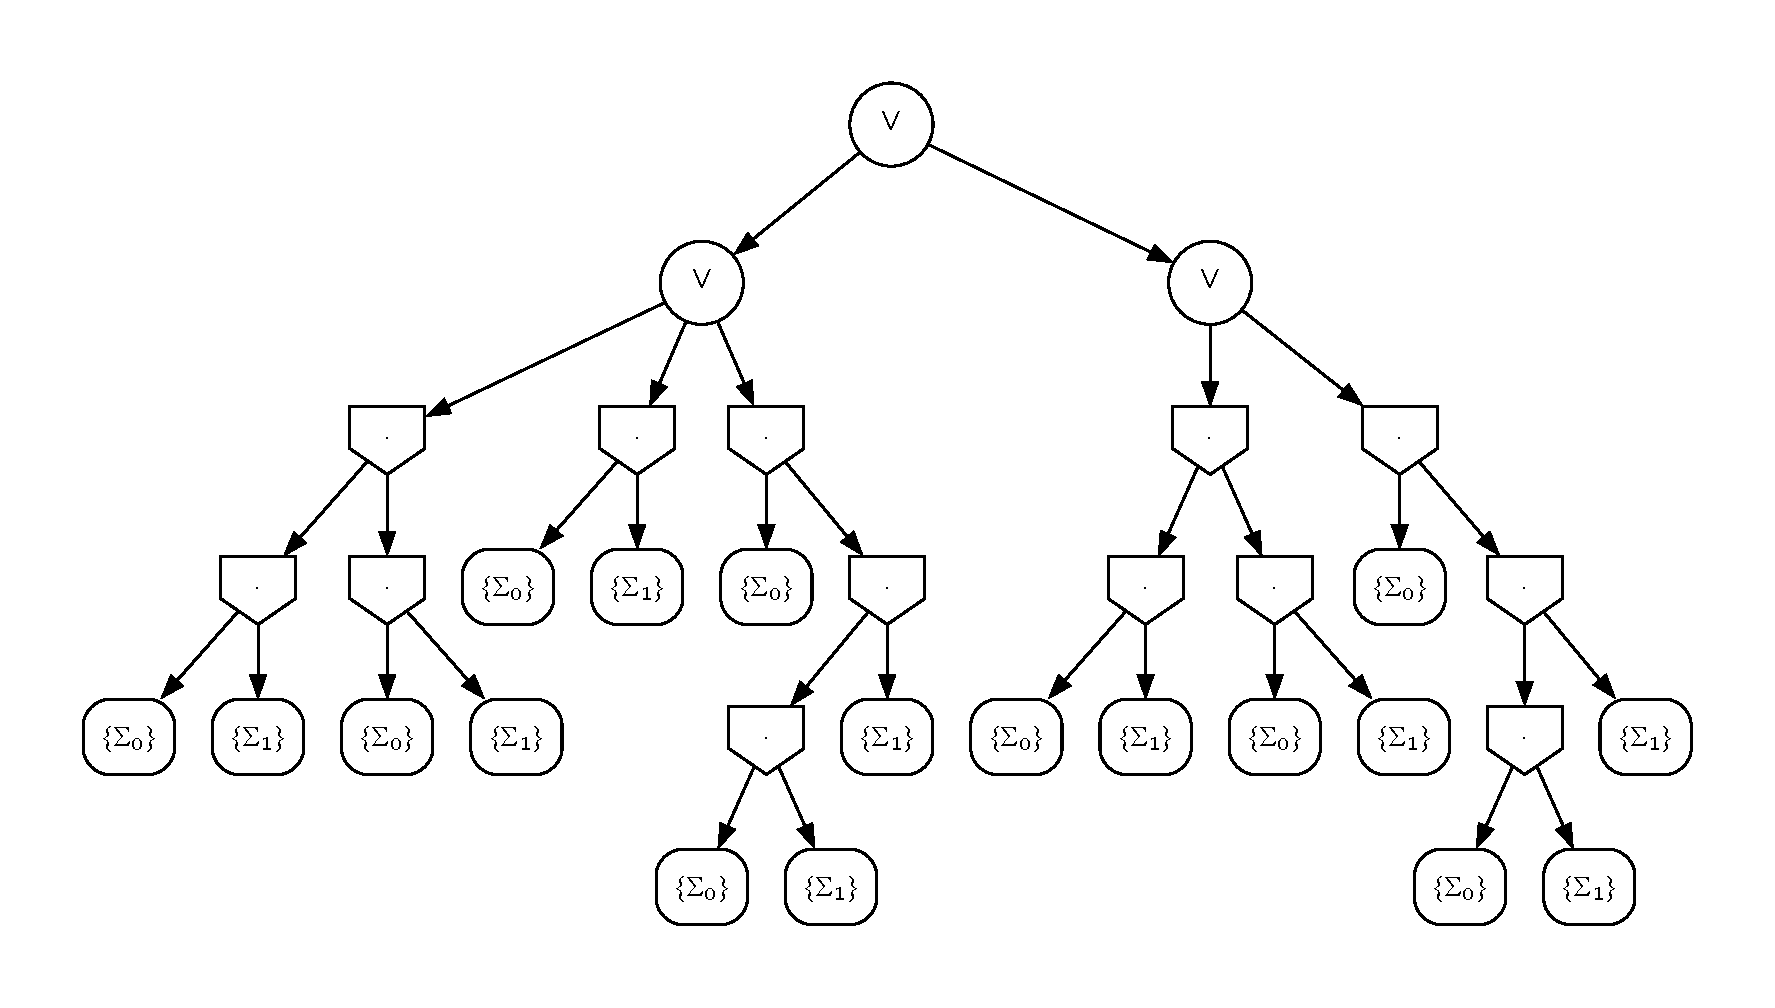
\includegraphics{figures/gre}
}
\end{center}
\vspace{-0.3cm}
\caption{Regular expression denoting $\mathcal{L}(G_\cap)$.}\label{fig:re_tree}
\end{wrapfigure}

As a concrete example, suppose we have the string, $\err\sigma=\texttt{())}$ and wish to balance the parentheses. We will initially have the Levenshtein automaton, $A$, depicted in Fig.~\ref{fig:ex_atm}. To check for non-emptiness, we will perform the following procedure. Suppose we have a CNF CFG, $G'= \big\{S \rightarrow L R, S \rightarrow L F, S \rightarrow S S, F \rightarrow S R, L \rightarrow \hspace{-0.05cm}\texttt{(}, R \rightarrow\hspace{-0.05cm}\texttt{)}\big\}$ and let us assume an ordering of $S, F, L, R$ on $V$.

First, we need to order the automata states by increasing longest-path distance from $q_0$. One approach would be to topologically sort the adjacency matrix. While some form of sorting is unavoidable for arbitrary ANFAs, if we know ahead of time that our structure is a Levenshtein automaton, we can simply enumerate its state space by increasing Manhattan distance from the origin. % using, e.g., the Cantor pairing function to construct a valid ordering. This ordering will form the row and column indices of our intersection matrix, and each entry will represent the existence of some path between a two states yielding a given nonterminal.
So, a valid ordering on $Q$ would be $q_{00}, q_{01}, q_{10}, q_{11}, q_{20}, q_{21}, q_{30}, q_{31}$. Now, we want to compute whether $[\mathcal{L}(G')\cap \mathcal{L}(A) \neq \varnothing]$.

Under such an ordering, the adjacency matrix takes an upper triangular form and becomes the template for the initial parse chart, $M_0$ (Fig.~\ref{fig:initial_pc}). Each entry of this chart corresponds to a vector of expressions $E^{|V|}$ with at least one expression denoting a nonempty language. Likewise, the reachability matrix signifies a subset of state pairs which can participate in the language intersection. The adjacency and reachability matrices will always cover the expression vectors of the initial and final parse charts, respectively. In other words, we may safely ignore absent $\langle q, q'\rangle$ pairs in the reachability matrix, as these state pairs definitely cannot participate in the intersection.

From the reachability matrix we can construct the parse chart via matrix exponentiation. We note that n-step reachability constraints n-step parseability, i.e., $\sum_{i=0}^n A^i[q, q'] = \ws \vdash M_n[q, q', v] = \ws$, thus we can avoid substantial work via memoization. In this example, since $M_\infty[q_{00}, q_{31}, S] = \bs$, this implies that $\mathcal{L}(A)\cap \mathcal{L}(G') \neq \varnothing$, hence $\text{LED}(\sigma, G) = 1$. Using the same matrix, we will then perform a second pass to construct regular expressions representing finite languages for each nonempty constituent. Once again, we can skip $\langle q, q', v\rangle$ entries when $M_\infty[q, q', v] = \ws$ to hasten convergence.

\enlargethispage{4\baselineskip}
Just as before, we will define $\boxplus, \boxtimes$ over GRE vectors, where $X \boxtimes Z = [X_x\cdot Z_z \mid (w\rightarrow xz) \in P]_{w\in V}$ and $X \boxplus Z= [ X_w\vee Z_w ]_{w\in V}$. Finally, we will repeat the matrix exponential, using $M_\infty$ in the binary domain as a guide. This allows us to construct the regular expression tree for $S_\cap = q_{00}Sq_{20}\vee q_{00}Sq_{31}$ shown in Fig.~\ref{fig:re_tree}. Once this regex is constructed, decoding becomes simply a matter of invoking \texttt{choose}$(S_\cap)$. In this case there are only a few choices, but in general, there can be a vast multitude.

\clearpage

\section{Measuring the language intersection}\label{sec:measurement}

We will now attempt to put a probability distribution over the language intersection. We shall start with a few cursory but illumative approaches, then proceed towards a more refined solution.

\subsection{Mode collapse}

Ordinarily, one might think to train a top-down PCFG sampler using a treebank of well-formed code snippets, however this method is highly degenerate in the finite case, exhibiting poor sample diversity. Consider an illustrative pathological case for top-down ancestral (TDA) sampling:
$$
G=\left\{ S \rightarrow A\:B \: \left(\frac{10^5 - 1}{10^5}\right), \hspace{2pt}
     S \rightarrow C\:C \: \left(\frac{1}{10^5}\right), \hspace{2pt}
     A \rightarrow a \: (1), \hspace{2pt}
     B  \rightarrow b \: (1), \hspace{2pt}
     C  \rightarrow a \: \left(\frac{1}{26}\right) \mid \ldots \mid z \: \left(\frac{1}{26}\right)\right\}
$$
Such a sampler will almost always yield $a b$, but most of $\mathcal{L}(G)$ is concealed in the hidden branch, $S \rightarrow C C$. Though a contrived example, it illustrates why TDA sampling is unviable: our sampler should match the true distribution over the finite CFL, not the PCFG's local approximation thereof.

\subsection{Exact enumeration}

To correct for mode collapse, a brute force solution would be to simply generate every tree. While the whole set can be materialized in some cases when the intersection language is small, this strategy is clearly suboptimal due to its worst-case complexity. Nevertheless, it is useful for checking completeness. To enumerate trees, we first need the total number of trees, which is denoted $|e|$.

\begin{definition}[Cardinality]
  $|e|: E \rightarrow \mathbb{N} =$ \begin{cases}
    1           & \text{if } e \in \Sigma \\
    x \times z  & \text{if } e = x \cdot z \\
    x + z       & \text{if } e = x \vee z
  \end{cases}\\
\end{definition}

\begin{theorem}[Enumeration]
  To enumerate, we can invoke $\bigcup_{i = 0}^{|R|}\{\texttt{enum}(R, i)\}$:\\

  $\texttt{enum}(e, n): E \times \mathbb{N} \rightarrow \Sigma^*$ = \begin{cases}
       e &\text{if } e \in \Sigma \\
       \texttt{enum}\big(x, \lfloor \frac{n}{|z|} \rfloor\big) \cdot \texttt{enum}\big(z,\, n \bmod |z|\big)  &\text{if } e = x \cdot z \\
       \texttt{enum}\big((x, z)_{\min(1, \lfloor\frac{n}{|x|}\rfloor)}, n-|x|\min(1, \lfloor\frac{n}{|x|}\rfloor)\big) &\text{if } e = x \vee z
  \end{cases}
\end{theorem}

This can be converted to a uniform sampler by drawing integers without replacement using a pseudorandom number generator, however, if $|e|$ is very large, \texttt{enum} can fail to capture modes.

\subsection{The problem with ambiguity}

The main problem with the previous approach is that it counts distinct trees, which overcounts the total number of words, $|\mathcal{L}(G_\cap)|$. Since the Levenshtein automaton can be ambiguous, this causes certain repairs to be overrepresented, resulting in a pernicious bias. Consider, for example,

\begin{lemma}\label{lemma:ambiguity}
If the FSA, $\alpha$, is ambiguous, then the intersection grammar, $G_\cap$, can be ambiguous.
\end{lemma}

\begin{proof}
Let $\ell$ be the language defined by $G=\{S\rightarrow LR, L \rightarrow\texttt{(}, R \rightarrow\texttt{)}\}$, where $\alpha=L(\err\sigma, 2)$, the broken string $\err\sigma$ is $\texttt{)(}$, and $\mathcal{L}(G_\cap) = \ell \cap \mathcal{L}(\alpha)$. Then, $\mathcal{L}(G_\cap)$ contains the following two identical repairs: \texttt{\hlred{)}(\hlgreen{)}} with the parse $S \rightarrow q_{00}Lq_{21}\phantom{.}q_{21}Rq_{22}$, and \texttt{\hlorange{(}\hlorange{)}} with the parse $S \rightarrow q_{00}Lq_{11}\phantom{.}q_{11}Rq_{22}$.
\end{proof}

\noindent We would expect the underlying sample space to be a proper set, \textit{not} a multiset.

\subsection{Disambiguation}\label{sec:transfer_method}

To count the number of distinct repairs, we will need to convert $G_\cap$ to an automaton. Since $\mathcal{L}(G_\cap)$ is finite, it must be regular a fortiori. Recalling the definition for an NFA, $\langle Q, \Sigma, \delta, q_\alpha: Q, F \subseteq Q \rangle$, and star-free regex, $e \rightarrow \Sigma \mid e \lor e \mid e \land e$, we will proceed by structural induction on the regex:

\begin{equation*}
N(e) =
\begin{cases}
  \begin{alignedat}{8}
    &\big\langle \{q_\alpha, q_\omega\}
    &&\,,\, \{ q_\alpha \overset{e}{\rightarrow} q_\omega \}
    &&\,,\, q_\alpha\,\,, \{q_{\omega}\}
    &&\big\rangle
    &&\:\: \text{if } e \in \Sigma \\[0.5em]

    &\big\langle Q_{x} \cup Q_{z}
    &&\,,\, \{ q \overset{s}{\rightarrow} q_{\alpha z} \mid (q \overset{s}{\rightarrow} q_{\omega}^{\in F_x}) \in \delta_x \} \cup \delta_{x} \cup \delta_{z}
    &&\,,\, q_{\alpha x}\,, F_{z}
    &&\big\rangle
    &&\:\: \text{if } e = x \cdot z \\[0.5em]

    &\Bigg\langle   \begin{matrix} Q_{x}\cup \{q_{\alpha e}\}\:\cup\\ Q_{z} \cup \{q_{\omega e}\}\phantom{\:\cup} \end{matrix}
    &&\,,\, \begin{matrix}\{ q_{\alpha e} \overset{s}{\rightarrow} q \mid (q_{\alpha x, \alpha z} \overset{s}{\rightarrow} q)\in \delta_{x, z} \} \cup \delta_{x}\:\cup\\
    \{ q \overset{s}{\rightarrow} q_{\omega e} \mid (q \overset{s}{\rightarrow} q_{\omega}^{\in F_{x,z}})\in \delta_{x, z} \}\cup \delta_{z}\phantom{\,\:\cup}\end{matrix}
    &&\,,\, q_{\alpha e}\,, \{q_{\omega e}\}
    &&\Bigg\rangle
    &&\:\:\text{if } e = x \lor z\hspace{-0.5cm}\\[-0.5em]
    \multicolumn{9}{c}{\tiny{\text{- - - - - - - - - - - - or - - - - - - - - - - - -}}} \\[-0.5em]
    &\big\langle Q_{x} \cup Q_{z} \cup \{q_{\alpha e}\}
    &&\,,\, \{ q_{\alpha e} \overset{s}{\rightarrow} q \mid (q_{\alpha x, \alpha z} \overset{s}{\rightarrow} q) \in \delta_{x, z} \}  \cup \delta_{x} \cup \delta_{z}
    &&\,,\, q_{\alpha e}\,, F_{x} \cup F_{z}
    &&\big\rangle
    &&\:\: \text{if } e = x \lor z
  \end{alignedat}
\end{cases}\vspace{0.2cm}
\end{equation*}

\noindent Though less conventional than Thompson's construction, $N(e)$ avoids the creation of unnecessary $\varepsilon$ arcs. And while slightly more verbose, we find the topology induced by the first version of the $\lor$ case to be more favorable for minimization. Continuing with our running example from \S~\ref{sec:repair_ex}, we will use Brzozowski's algorithm~\cite{brzozowski1962canonical} to construct the unique minimal DFA, $D^*_\cap \equiv_\mathcal{L} G_\cap$: \vspace{-0.4cm}

\begin{figure}[H]
  \centering
  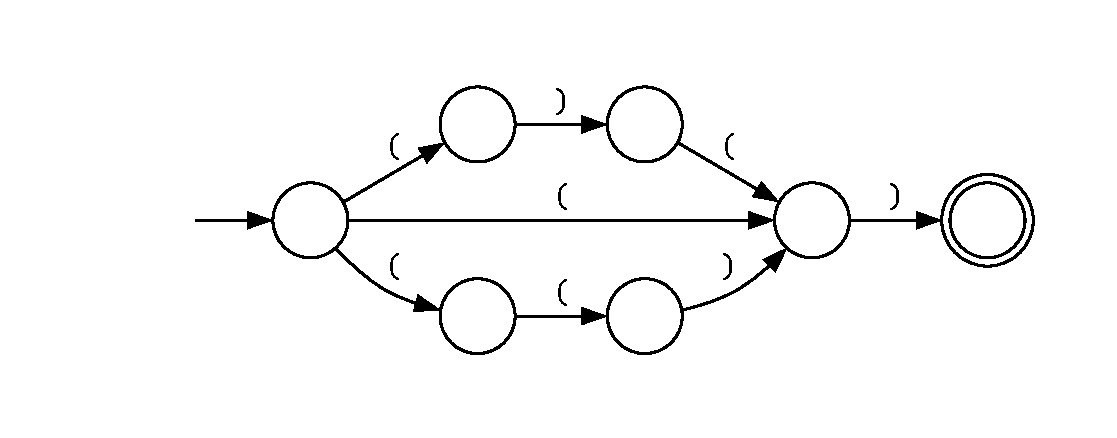
\includegraphics[width=0.27\textwidth]{figures/dyck_nfa}
  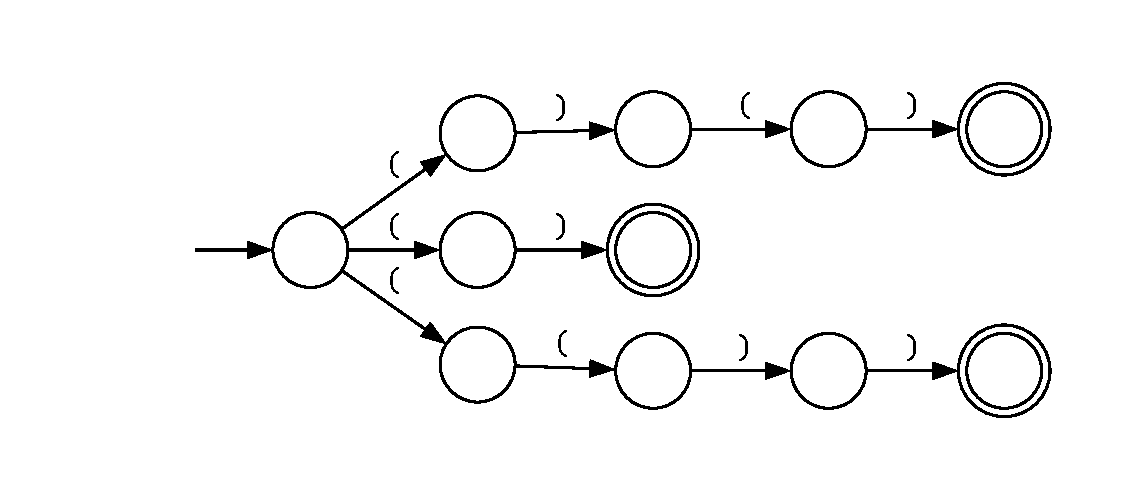
\includegraphics[width=0.27\textwidth]{figures/dyck_nfa_orig}
  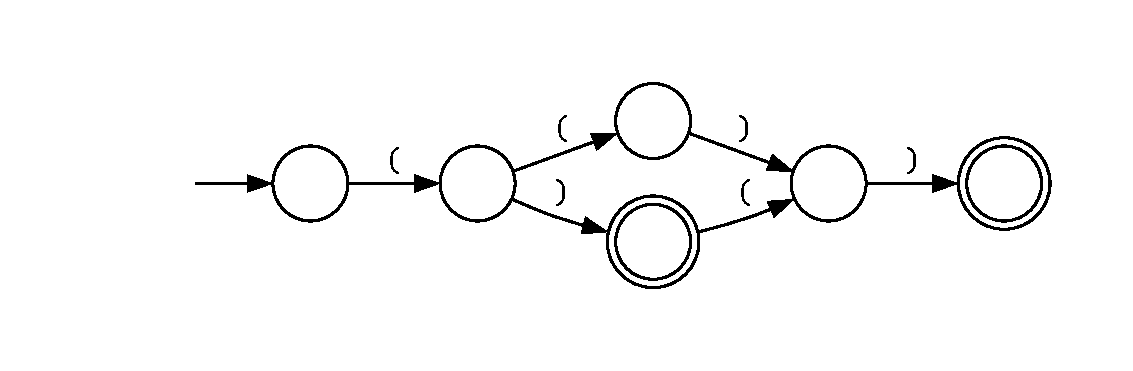
\includegraphics[width=0.30\textwidth]{figures/dyck_dfa}
  \vspace{-0.2cm}
  \caption{FSA for $\mathcal{L}\big(L(\texttt{())}, 1)\big)\cap\mathcal{L}(G')$ (a) with or (b) without $\lor$-merging, and then (c) post-minimization.}\label{fig:fsas_for_re}
  \vspace{-0.2cm}
\end{figure}
Since $\mathcal{L}(G_\cap)$ is necessarily finite, we can infer that the corresponding DFA is acyclic and thus representable as an upper triangular adjacency matrix under a topological ordering of $\delta$. For any such DFA, we can ascertain the size of its language by counting walks from $q_\alpha$ to $q_\omega \in F$. Letting $A$ be the adjacency matrix for $D_\cap^*$, i.e., $A[q, q'] = \big[1 \text{ if } \exists s: \Sigma \text{ s.t. } (q \overset{s}{\rightarrow} q') \in \delta \text{ else } 0\big]$, the number of words it recognizes is given via the transfer matrix method~\cite{flajolet2009analytic}, that is,
\begin{align}
  C(A, q_\alpha, F): \mathbb{N}^{|Q|\times|Q|} \times Q \times 2^Q \rightarrow \mathbb{N} = \sum_{\mathclap{q_\omega \in F}}(I-A)^{-1}[q_\alpha, q_\omega] &= \sum_{\mathclap{q_\omega \in F}}\sum_{i = 0}^{\mathclap{|Q|-1}}A^i[q_\alpha, q_\omega]
\end{align}
\noindent Plugging in powers of the adjacency matrix for the DFA shown in Fig.~\ref{fig:fsas_for_re}.(c), we arrive at the total:
\begin{align}
(I-A)^{-1} &= \hspace{1cm}I + A \hspace{1cm}+\hspace{1.05cm} A^2 \hspace{1.07cm}+\hspace{1cm} A^3 \hspace{0.9cm}+\hspace{0.9cm} A^4\\
  &=\begin{tiny}\begin{pmatrix}
       1 & 1 &   &   &   &   \\
        & 1  & 1 & 1 &   &   \\
        &   & 1  &   & 1 &   \\
        &   &   & 1  & 1 &   \\
        &   &   &   & 1  & 1 \\
        &   &   &   &   & 1  \\
  \end{pmatrix} + \begin{pmatrix}
              &   & 1 & 1 &   &   \\
              &   &   &   & 2 &   \\
              &   &   &   &   & 1 \\
              &   &   &   &   & 1 \\
              &   &   &   &   &   \\
              &   &   &   &   &   \\
  \end{pmatrix} + \begin{pmatrix}
              &   &   &   & 2 &   \\
              &   &   &   &   & 2 \\
              &   &   &   &   &   \\
              &   &   &   &   &   \\
              &   &   &   &   &   \\
              &   &   &   &   &   \\
  \end{pmatrix} + \begin{pmatrix}
              &   &   &   &   & 2 \\
              &   &   &   &   &   \\
              &   &   &   &   &   \\
              &   &   &   &   &   \\
              &   &   &   &   &   \\
              &   &   &   &   &   \\
  \end{pmatrix}\end{tiny}\\
  &= \begin{tiny}\begin{pmatrix}
          1   & 1  & 1  & \underline{1} & 2 & \underline{2} \\
              & 1  & 1  & 1 & 2 & 2 \\
              &    & 1  &   & 1 & 1 \\
              &    &    & 1 & 1 & 1 \\
              &    &    &   & 1 & 1 \\
              &    &    &   &   & 1 \\
\end{pmatrix}\end{tiny} \text{ therefor, } \big|\mathcal{L}(D_\cap^*)\big| = C\big(A, q_0, \{q_3, q_5\}\big) = \underline{1} + \underline{2} = 3.
\end{align}
Note the model counting problem is strictly harder than deciding intersection nonemptiness as it requires a secondary determinization step, however, weak bounds may be obtained by applying $C$ to the automaton generated by $N(e)$ or by direct analysis of $e$. While the inequality $C_{D_\cap^*} \leq C_{N(e)} \leq |e|$ will hold, the bounds provided by the latter approximations may be vacuous, whereas $C_{D_\cap^*}$ is exact.

%The advantage of dealing with formal language representations is that we can reason about them algebraically. Consider the context-free grammar: the arrow $\rightarrow$ becomes an $=$ sign, $\mid$ becomes $+$ and $AB$ becomes $A \times B$. The ambiguous Dyck grammar, then, can be seen as a system of equations.
%
%\begin{equation}
%  S \rightarrow ( ) \mid ( S ) \mid S S \Longleftrightarrow f(x) = x^2 + x^2 f(x) + f(x)^2
%\end{equation}
%
%\noindent We will now solve for $f(x)$, giving us the generating function for the language:
%
%\begin{equation}
%  0 = f(x)^2 + x^2 f(x) - f(x) + x^2
%\end{equation}
%
%\noindent Now, using the quadratic equation, where $a = 1, b = x^2 - 1, c = x^2$, we have:
%
%\begin{equation}
%  f(x) = \frac{-b \pm \sqrt{b^2 - 4ac}}{2a} = \frac{-x^2 + 1 \pm \sqrt{x^4 - 6x^2 + 1}}{2}
%\end{equation}
%
%\noindent Note there are two solutions, but only one where $\lim_{x\rightarrow 0} = 1$. From the ordinary generating function (OGF), we also have that $f(x)=\sum _{n=0}^{\infty }f_nx^{n}$. Expanding $\sqrt{x^4 - 6x^2 + 1}$ via the generalized binomial theorem, we have:
%
%\begin{align}
%  f(x) = (1+u)^{\alpha }&=\sum _{k=0}^{\infty }\;{\binom {\alpha }{k}}\;u^{k}\\
%  &=\sum _{k=0}^{\infty }\;{\binom {\frac{1}{2} }{k}}\;(x^4 - 6x^2)^{k} \text{ where } u = x^4-6x^2
%\end{align}
%
%Now, to obtain the number of ambiguous Dyck trees of size $n$, we can extract the $x^n$-th coefficient using the binomial series:
%
%\begin{align}
%[x^n]f(x) &= [x^n]\frac{-x^2 + 1}{2} + \frac{1}{2}[x^n]\sum _{k=0}^{\infty }\;{\binom {\frac{1}{2} }{k}}\;(x^4 - 6x^2)^{k}\\
%[x^n]f(x) &= \frac{1}{2}{\binom {\frac{1}{2} }{n}}\;[x^n](x^4 - 6x^2)^n = \frac{1}{2}{\binom {\frac{1}{2} }{n}}\;[x^n](x^2 - 6x)^n
%\end{align}
%
%We can use this technique, first described by Flajolet \& Sedgewick~\cite{flajolet2009analytic}, to count the number of trees of a given size or distinct words in an unambiguous CFG. This lets us understand grammars as a kind of algebra, which is useful for enumerative combinatorics on words and syntax-guided synthesis. We use use this in our setting to count the total number of words in the intersection grammar.

\clearpage\section{Implementation}\label{sec:implementation}

The implementation essentially consists of four stages, each dependent on its predecessor.

\begin{enumerate}
  \item $\texttt{lev\_build}: \Sigma^{|Q|-1} \times \mathbb{N}^{3} \rightarrow \text{NFA}$ -- constructs a Levenshtein NFA from the broken string.
  \item $\texttt{cfl\_fixpt}: \text{NFA} \times \text{CFG} \rightarrow \mathbb{B}^{|Q|\times |Q| \times |V|}$ -- computes the matrix exponential.
  \item $\texttt{reg\_build}: \mathbb{B}^{|Q|\times |Q| \times |V|} \times \text{CFG} \rightarrow \text{GRE}$ -- constructs the regular expression for $G_\cap$.
  \item $\texttt{reg\_dcode}: \text{GRE} \times \mathbb{N}^{|\Sigma|^{c\approx 3}} \hspace{-0.05cm}\times \mathbb{N} \rightarrow\hspace{-0.02cm} (\Sigma^+)^{k\approx 10}$ -- returns a small set of the most probable repairs.
%  \item $\texttt{sel\_top\_k}: (\Sigma^* \times \mathbb{N})^{p\gg1} \times \mathbb{N} \rightarrow (\Sigma^*)^{k\ll p}$ -- returns a small set of the most probable repairs.
\end{enumerate}

\noindent We will now explore the imperative pseudocode for each stage, starting with the Levenshtein automata constructor, which is a straightforward translation of the inference rules in \S~\ref{sec:repair_ex}.

\begin{algorithm}[H]
\caption{\texttt{lev\_build} pseudocode}
\label{alg:lev_build}
\begin{algorithmic}[1]
  \Procedure{\texttt{lev\_build}$(\sigma: \Sigma^n, d_{\max}: \mathbb{N})$}{} \Comment{Takes a string and maximum edit distance.}
  \State $Q, \delta \gets \varnothing$
  \For{$\langle h, j, i, k \rangle \textbf{ in } [0, n]^2\times[0, d_{\max}]^2$\vspace{1.34cm}}
    \State \vspace{-1.65cm}\[\hspace{1.15cm}\delta\,\gets \delta\,\cup\:\!\left\{
        \begin{alignedat}{9}
          &\;& q_{h,i} &\hspace{-0.1cm}\overset{{\color{orange}[\neq\sigma_{j+1}]}}{\rightarrow} &q_{j,k} &\qquad& \text{if}\;& h = j   &\:\land\:& i = k-1  &\qquad& \duparrow\\[-2pt]
          && q_{h,i}   &\overset{{\color{orange}[\neq\sigma_j]}}{\rightarrow} &q_{j,k} &&       \text{if}\;& h = j-1 &\:\land\:& i = k-1  &&       \ddiagarrow\\[-2pt]
          && q_{h,i}   &\overset{{\color{orange}[=\sigma_j]}}{\rightarrow}    &q_{j,k} &&       \text{if}\;& h = j-1 &\:\land\:& i = k    &&       \drightarrow\\[-2pt]
          && q_{h,i}   &\overset{{\color{orange}[=\sigma_j]}}{\rightarrow}    &q_{j,k} &&       \text{if}\;& 1 \leq j - h - 1 \leq d_{\max} &\:\land\:& 1 \leq k - i \leq d_{\max}   && \knightarrow\;
        \end{alignedat}
      \right\}\]
    \State $Q \gets Q \cup \{q_{h,i}, q_{j,k}\}$
  \EndFor
  \State $I \gets \{q_{0,0}\}, F \gets \{q_{i, j} \mid n - i + j \leq d_{\max}\}$
  \State \Return $\langle Q, \Sigma, \delta = Q \times (\Sigma\:{\color{orange}\rightarrow \mathbb{B}}) \times Q, q_\alpha, F\rangle$  \Comment{Returns a [nominal] Levenshtein automaton.}
\end{algorithmic}
\end{algorithm}\vspace{-0.2cm}

Next, the chart parser expects an acyclic NFA, a CNF grammar and returns a Boolean 3-tensor.

\begin{algorithm}[H]
\caption{\texttt{cfl\_fixpt} pseudocode}
\label{alg:cfl_fixpt}
\begin{algorithmic}[1]
\Require CFG must be in CNF and the NFA must be $\varepsilon$-free and acyclic (i.e., denote a finite langauge).
\Procedure{\texttt{cfl\_fixpt}$\big(\langle \Sigma, V, P, S\rangle: \text{CFG}, \langle Q, \Sigma, \delta, q_\alpha, F\rangle: \text{NFA}\big)$}{}
\State $R: \mathbb{B}^{|Q|\times |Q|} \gets \big[\bs \textbf{ if } \exists \sigma \in \Sigma^+ \mid q \overset{\sigma}{\rightsquigarrow} q' \textbf{ else } \ws\big]_{q,\,q'\,:\, Q}$ \Comment{Solve for reachability matrix.}
\State $M: \mathbb{B}^{|Q|\times |Q| \times |V|} \gets \big[\bs \textbf{ if } \exists s: \Sigma \mid (v \rightarrow s) \in P \land (q \overset{{\color{orange}\varphi}}{\rightarrow} q') \in \delta \land {\color{orange}\varphi(}s{\color{orange})} \textbf{ else } \ws\big]_{q,\,q'\,:\,Q,\,v\,:\,V}$
\For{$i \textbf{ in } \big[0, \lceil\log_2(|Q||V|)\rceil\big]$} \Comment{Solves matrix exponential, $\exp(M_0)$.}
\State $\textsc{done} \gets \bs$
\For{$\langle p, r, w \rangle \textbf{ in } Q^2\times V$} \Comment{Iterates one step of $M_{i+1} = M_i + M_i^2$.}
  \State $\textbf{if } M[p, r, w] \textbf{ or not } R[p, r] \textbf{ then continue}$
  \State $Q_{pr} \gets \big\{q: Q \mid R[p, q] \land R[q, r]\big\}$ \Comment{Consider reachable states between p and r.}
  \State $M[p, r, w] \gets \bs \textbf{ if } \exists q: Q_{pr}, x, z: V \mid M[p, q, x] \land M[q, r, z] \land (w \rightarrow x z) \in P \textbf { else } \ws$
  \State $\textbf{if } M[p, r, w] \textbf{ then } \textsc{done} \gets \ws$
\EndFor
\State $\textbf{if }\textsc{done} \textbf{ then break}$
\EndFor
\State \Return $M$ \Comment{Returns the completed Boolean parse chart.}
  \end{algorithmic}
\end{algorithm}\vspace{-0.2cm}

Note we may short-circuit for three reasons, if: $M_{i+1} = M_i$, when two states $q, q'$ are unreachable, or whenever a $\langle q, q', v\rangle$ is already present. Once we obtain $M_\infty$, we can immediately tell whether $\ell_\cap \neq \varnothing$ by checking whether $M_\infty[q_\alpha, q_\omega, S] = \bs$ for some $q_\omega: F$. Otherwise if no such $q_\omega$ exists, then $\ell_\cap$ must be empty and $d_\max$ should be enlarged before proceeding.

Now we can perform a second sweep over nonempty entries of the Boolean parse chart, reconstructing the provenance of each $\langle q, q', v\rangle$ constituent. For compactness it will be convenient to use a pointer-based representation of the regular expression instead of manipulating strings.

\begin{algorithm}[H]
\caption{\texttt{reg\_build} pseudocode}
\label{alg:reg_build}
\begin{algorithmic}[1]
  \Require Same as \texttt{cfl\_fixpt} (Alg.~\ref{alg:cfl_fixpt}), $M_{\mathbb{B}}[q_\alpha, q_\omega: F, S] = \bs$ for some $q_\omega$, and $M_{\mathbb{B}} = M_{\mathbb{B}} + M_{\mathbb{B}}^2$.
  \Procedure{\texttt{reg\_build}$\big(M_{\mathbb{B}}: \mathbb{B}^{|Q|\times |Q| \times |V|}, \langle \Sigma, V, P, S\rangle: \text{CFG}, \langle Q, \Sigma, \delta, q_\alpha, F\rangle: \text{NFA}\big)$}{}
  \State $P: \mathbb{B}^{|Q|\times |Q|} \gets \big[\bs \textbf{ if } \exists q: Q, v, v': V \mid M_{\mathbb{B}}[p, q, v] \land M_{\mathbb{B}}[q, r, v'] \textbf{ else } \ws\big]_{p,\,r\,:\,Q}$
  \State $M: \text{GRE}^{|Q|\times |Q| \times |V|} \gets \big[\{s: \Sigma \mid M[q, q', v] \land (q \overset{{\color{orange}\varphi}}{\rightarrow} q') \in \delta \land (v\rightarrow s) \in P \land {\color{orange}\varphi(}s{\color{orange})}\}\big]_{q,\,q'\,:\, Q,\,v\,:\,V}$
  \For{$i \textbf{ in } \big[0, \lceil\log_2(|Q||V|)\rceil\big]$}
  \State $M' \gets M$
  \For{$\langle p, r, w \rangle \textbf{ in } Q^2\times V$}
  \State $\textbf{if not } M_\mathbb{B}[p, r, w] \textbf{ then continue}$
  \State $Q_{pr} \gets \big\{q: Q \mid P[p, q] \land P[q, r]\big\}$ \Comment{Consider parseable states between p and r.}\vspace{0.2cm}
  \State \vspace{-0.42cm}\[\hspace{0.62cm}M'[p, r, w] \gets M[p, r, w] \vee \bigvee_{\mathclap{\substack{q\,:\,Q_{pr}\\x,\,z\,:\,V}}} \big\{M[p, q, x]\cdot M[q, r, z] \mid (w \rightarrow x z) \in P\big\}\]\vspace{-0.2cm}
  \EndFor
  \State $\textbf{if } M=M' \textbf{ then break else } M \gets M'$
  \EndFor \vspace{0.2cm}
  \State \vspace{-0.42cm}\[\hspace{-8.5cm}\textbf{return }\bigvee_{\mathclap{q_\omega\,:\,F}} M[q_\alpha, q_\omega, S]\vspace{-0.8cm}\] \Comment{Union regexes for all total parses yielding S.}\vspace{0.31cm}
\end{algorithmic}
\end{algorithm}

Finally, once we have the expression for $G_\cap$, we can decode it to extract a small set of candidates. Various strategies are possible here, and we opt for the simplest one. We use two priority queues to store partial and total trajectories, which are ranked by probability as estimated by a pretrained c-gram count tensor, $C$. Partial trajectories are greedily extended until termination, after which the trajectory it is diverted to the total queue, and the top-k total trajectories are returned.

\begin{algorithm}[H]
  \caption{\texttt{reg\_dcode} pseudocode}
  \label{alg:reg_dcode}
  \begin{algorithmic}[1]
  \Require We expect the shortest word to exceed the Markov order in length, $c < |\sigma|, \forall\sigma: \mathcal{L}(e)$.
  \Procedure{\texttt{reg\_dcode}$\big(e: \text{GRE}, C: \mathbb{N}^{|\Sigma|^{c\approx 3}}, k: \mathbb{N}\big)$}{}
    \State $\mathcal{T} \gets [], \mathcal{E} \gets \big[\langle \varepsilon^{c-1}, e\cdot \varepsilon^{c-1}, 0\rangle\big]$ \Comment{Initialize total and partial trajectories.}\vspace{0.5cm}
    \State \vspace{-0.55cm}\[\hspace{-4.58cm}\textbf{let } P(s: \Sigma \mid \sigma: \Sigma^{\geq c-1}) = \frac{C[\sigma_{|\sigma| - c + 1, |\sigma|}\cdot s]+ 1}{\sum_{s' \in \Sigma} C[\sigma_{|\sigma| - c + 1, |\sigma|}\cdot s']}\vspace{-0.7cm}\]\Comment{Define Markov transition probability.}\vspace{0.3cm}
    \Repeat
        \State $\langle\sigma, e, p\rangle \gets \textbf{pop } \mathcal{E}_0 \textbf{ off }\mathcal{E}$
        \State $\mathcal{E}' \gets \big[\langle\sigma\cdot a, \partial_a e, p + \ln P(a\mid \sigma) \rangle \mid a \in \texttt{follow}(e)\big]$
        \State $\mathcal{T}\hspace{0.05cm} \gets \mathcal{T} \texttt{++} \big[\langle \sigma, p \rangle \mid \langle \sigma, e, p\rangle \in \mathcal{E}' \land \varepsilon \in \mathcal{L}(e)\big]$
        \State $\mathcal{E}\phantom{'} \gets \big[\langle\sigma, e, p\rangle \in (\mathcal{E} \texttt{++} \mathcal{E}')\textbf{ sorted by } p\big]$
    \Until{interrupted or $\mathcal{E}$ is empty.}
    \State \Return $[\sigma \mid \langle\sigma, p\rangle \in \mathcal{T}_{0..k}\textbf{ sorted by } p]$ \Comment{Skim off top-k repairs by c-gram probability.}
  \end{algorithmic}
\end{algorithm}

%Now we are ready to skim off the highest probability repairs using a standard selection algorithm.
%
%\begin{algorithm}[H]
%  \caption{\texttt{sel\_top\_k} pseudocode}
%  \label{alg:sel_top_k}
%  \begin{algorithmic}[1]
%    \Procedure{\texttt{sel\_top\_k}$\big(l: (\Sigma^* \times \mathbb{N})^{p\gg1}, k: \mathbb{N}\big)$}{}
%    \State $\hat{A}: (\Sigma^* \times \mathbb{N})^* \gets [l_0]}$ \Comment{Initialize a priority queue of nearly-optimal repairs.}
%    \For{$\langle\sigma, s\rangle \textbf{ in } l$}
%      \State $\textbf{if } s < \pi_2(\hat{A}_{|\hat{A}|}) \textbf{ then insert } \langle\sigma, s\rangle \textbf{ into } \hat{A} \textbf{ and drop } \hat{A}_{|k + 1|} \textbf{ if } |\hat{A}| > k$
%    \EndFor
%    \State \Return $[\pi_1(a) \mid a \in \hat{A}]$ \Comment{Return top-k candidates.}
%  \end{algorithmic}
%\end{algorithm}

  Now, we have our shortlist of repairs and after cosmetic postprocessing, can present them to the user. With this approach, we can quickly generate a representative subset of $\ell_\cap$ within a fixed latency budget, e.g., \~100ms, or otherwise terminate early should we succeed in exhaustively generating it.

\clearpage\subsection{GPU translation}

This architecture can be translated to series of high-performance GPU kernels, essentially binary tensor contractions which are optimized for GPU acceleration. Our strategy will be to treat each stage of the repair pipeline as a massively parallel map-reduce job. Each thread will be responsible for writing a single entry to a large buffer, independently and without external communication.

We will make the simplifying assumption that each GPU kernel is a pure function that takes as input a coordinate triple $r, c, v: \mathbb{N}$ and one or more flat buffers $b_1: \mathbb{N}^{d_1}, \ldots b_n: \mathbb{N}^{d_n}$ containing encoded data, does some arithmetic, and returns a single output buffer, $b_{\text{out}}: \mathbb{N}^{d}$. The main challenge of GPU programming then becomes mapping aggregate datatypes to and from an integer format.

Morally, each $\langle r, c, v\rangle$ triple will dispatch a single isolated GPU thread with global read access to the input buffers and exclusive write access to a contiguous region of the output buffer. Absent a GPU, this can be rewritten as a triply-nested loop, subject to additional latency overhead. Each thread is effectively executed simultaneously on a GPU, but all memory must be sized ahead of time, as dynamic allocation is forbidden during a GPU kernel's execution. This presents a minor challenge for constructing the GRE datatype, though surmountable with careful reference counting.

For the CFG and NFA datatypes, we elect to use a dense representation $\mathbb{B}^{|V|\times|V|\times|V|}$ and $\mathbb{B}^{|Q|\times|Q|\times |\Sigma|}$ due to the tripartite coordinate structure and thread dispatching API. While these datatypes can be encoded sparsely as $\mathbb{N}^{3|P|}$ and $\mathbb{N}^{3|\delta|}$, for most repair instances and memory configurations representation size is not a bottleneck. It will be helpful to define two indices $\texttt{nt\_enc}: \Sigma \rightarrow 2^V$ and $\texttt{nt\_dec}: V \rightarrow 2^\Sigma$ for nonterminal encoding and decoding, and bijections $\Sigma \leftrightarrow \mathbb{N}$, $V \leftrightarrow \mathbb{N}$ for getting into and out of the integer domain -- these we omit for brevity but are trivial to define.

The parse chart $M$ can be represented as a bit-packed integer matrix $\texttt{uint32}^{|Q|\times|Q|\times|V|}$, whose layout testifies to four properties of each $\langle q, q', v\rangle$ triple: (1) the first bit encodes the dis/equality predicate ${\color{orange}\varphi}}$, (2) the next 25 bits designate terminal participation $\big(\text{if }\exists s: \Sigma. \varphi(s) \land (q \overset{{\color{orange}\varphi}}{\rightarrow} q')\in \delta\big)$, (3)~the next five bits memoize the minimum $i_{\min}$ such that $M_{i_{\min}}[q, q', v] \& 1 = \bs$ for short-circuiting (see Line \#7 of Alg.~\ref{alg:reg_build}), and (4) the lowest-order bit denotes parsability, i.e., $q\rightsquigarrow q'\vdash v$. Note the decoder must acknowledge the possibility that $v$ can simultaneously parse (a) an arc $q\rightarrow q'$ and (b) a path $q\rightsquigarrow q'$, so each branch can be explored. This is depicted below in little-endian format:\vspace{-0.1cm}

\[
\big[\overset{\overset{{\color{orange}=/\neq}}{\Updownarrow}}{\bs}, \overbrace{\ws, \ws, \ldots, \bs, \ws, \bs}^{s:\:\Sigma \Leftrightarrow \mathbb{B}^{25}}, \overbrace{\ws, \ws, \ws, \ws, \bs}^{i_{\min}:\:\mathbb{N}_{\leq 32}\Leftrightarrow \mathbb{B}^{5}}, \overset{\overset{v:\:V}{\Updownarrow}}{\bs}\big]: \texttt{uint32}
\]

Once \texttt{cfl\_fixpt} (Alg.~\ref{alg:cfl_fixpt}) is complete, we can calculate the total amount of memory needed to allocate $G_\cap$ by counting constituents in the parse chart. Being an algebraic datatype, the GRE datatype can be flattened in various ways. We will use the following memory layout,\vspace{-0.1cm}

\[
\big[\overbrace{\underset{\texttt{bp}_0}{2}, \underset{\texttt{bp}_1}{7}, \ldots, \underset{\texttt{bp}_{c-2}}{1}, \underset{\texttt{bp}_{c-1}}{3}}^{\texttt{bp\_counts}}, \overbrace{0, 4, \ldots, \underset{\texttt{bp}_{c-2}}{n-8}, \underset{\texttt{bp}_{c-1}}{n-6}}^{\texttt{bp\_offsets}}, \overbrace{\underbrace{\underline{59,83}, \underline{64, 152}}_{\texttt{bp}_0}, \ldots, \underbrace{\underline{34, 83}}_{\texttt{bp}_{c-2}}, \underbrace{\underline{22,74},  \underline{74, 90}, \underline{16, 66}}_{\texttt{bp}_{c-1}}}^{\texttt{bp\_storage}}\big]:  \texttt{uint32}^n
\]

\noindent where each $\texttt{bp}_i$ represents a nonempty $\langle q, q', v\rangle$ constituent with at least one back-pointer pair, $\texttt{bp\_count}(p, r, w) = \big|\big\{\langle q, x, z\rangle\mid  M[p, q, x] \land M[q, r, z] \land (w \rightarrow xz)\in P\big\}\big|$ counts the number of unique backpointers held by each nonterminal $w$ parseable from $p \rightsquigarrow r$, and $\texttt{bp\_storage}$ stores pointers to memory locations in the same data structure. These pointers should also be tied to locations in the parse chart $M[q, q', v]$ to recover the terminal subsets for unit productions.

In total, the GPU should have at least 4 GB of onboard memory to accommodate language intersections with up to 1k states and nonterminals $\big(|Q|^2\times|V|=10^6\times10^3\times 32 \text{ bits} \approx \text{4 GB}\big)$, however occupancy can be roughly halved by exploiting the upper-triangular structure of $M$.

\clearpage\subsection{Training the reranker}

Decoding returns a list of repair candidates that are all valid, nearby and at least somewhat plausible, however it is possible this list may be quite long. No reasonable user would be expected to skim through more than a few dozen candidates to select their intended repair, especially since they could have easily written it themselves in a few seconds. So, we will sort this list by a reranking model. As long as we can guarantee the documents are sufficiently exhaustive, they should with high probability include the true repair, which then need only be surfaced to the top of the list.

The ensuing method falls under the umbrella of the \textit{learning-to-rank} (LTR) problem in machine learning -- using their terminology, the broken code snippet would be called a \textit{query} and the list of repairs, \textit{documents}. To introduce the reranker, we must now overload some concepts, so the reader is trusted to contextually interpret $\mathcal{L}$ as denoting a \textit{loss} instead of a langauge, and the derivative~\footnote{There is a connection to Brzozowski's derivative, but to refrain from digression here we refer the reader to ~\cite{elliott2019generalized} for details.} as the directional rate of change of a differentiable manifold over the parameter space of a neural network. Matrix multiplication remains more or less the same, except now over the reals.

The reranker employs a transformer-encoder architecture to map both the query (broken code snippet, denoted $\err\sigma: \bar\ell$) and the document (candidate repair, denoted $\sigma: \ell_\cap$) to a $k$-dimensional real vector space $\mathbb{R}^k$. We elide the definition of a transformer-encoder (see Strobl et al.'s survey~\cite{strobl2024formal}), except to say that it is a function, $\text{E}_\theta$, which takes a string and a positional encoding, and returns an embedding, $\text{E}_\theta: (\Sigma\times \mathbb{N})^n \rightarrow \mathbb{R}^k$ where $\theta$ are learnable parameters. To these, we will introduce a third argument, a Levenshtein alignment $(\text{LA}: \Sigma^n \times \Sigma^m \rightarrow \mathbb{N}^{\max(m, n)})$, which, when applied to a query-document pair will produce a vector that tracks edit locations and types. Finally, a multilayer perceptron $(\text{MLP}_\theta: \mathbb{R}^k \rightarrow \mathbb{R}^+)$ processes the embedding to produce a relevance score:


\[
f_\theta(\err\sigma, \sigma): \bar\ell \times \ell_\cap \rightarrow \mathbb{R}^+ = \text{MLP}_{\theta}\Big(\text{E}_\theta\big(\err\sigma \cdot \sigma, 0\ldots <|\err\sigma|\cdot 0\ldots <|\sigma|, 0^n\cdot\text{LA}(\err\sigma, \sigma)\big)\Big)
\]

\noindent The training objective is to minimize the tempered \textit{softmax} or listwise cross-entropy loss,

\begin{equation}
\mathcal{L}(\theta) = -\sum_{q \in \mathcal{Q}} \log \left( \frac{\exp\big(f_\theta(q, d^*)\tau^{-1}\big)}{\sum_{d \in \mathcal{D}_q} \exp\big(f_\theta(q, d)\tau^{-1}\big)} \right)
\end{equation}

\noindent where $\mathcal{Q}$ is the set of training queries, $\mathcal{D}_q$ is the set of candidate repairs for query $q$, and $d^* \in \mathcal{D}_q$ is true repair. The temperature parameter, $\tau$ controls the sharpness of the softmax distribution, encouraging parameter settings that result in the the true repair being assigned higher priority -- the closer to zero, the greater the loss will be for underestimating the relevance of the true repair.

%The full parameters $\theta$ are partitioned into two sets, $\theta_e, \theta_r$, for the encoder and reranker layers. The encoder will be pretrained on next-token prediction, then fine tuned on the reranking task. During optimization, we use a smaller learning rate ($\alpha = 10^{-5}$) so as not to disturb the pretrained encoder parameters and a larger learning rate ($\alpha = 10^{-4}$) for the reranker parameters.

\begin{wrapfigure}{r}{0.40\textwidth}\vspace{-0.3cm}
\resizebox{0.4\textwidth}{!}{%
\begin{equation*}
  \begin{array}{r@{\hskip 0.5em}c|ccccccc}
    \text{$q$:}         & & \texttt{NAME} & \texttt{=} & \texttt{NAME} & \texttt{)} & \texttt{NAME} & & \\
    \text{PE:} & & 0 & 1 & 2 & 3 & 4 & & \\\hline
    \text{$d_1$:}  & & \texttt{NAME} & \texttt{=} & \texttt{NAME} & \hlorange{\texttt{(}} & \texttt{NAME} &  \hlgreen{\texttt{)}} & \\
    \text{PE:} & & 0 & 1 & 2 & 3 & 4 & 5 &\\
    \text{LA:} & & 0 & 0 & 0 & 2 & 0 & 1 &\\\hline
    \text{$d_2$:}  & & \texttt{NAME} & \hlorange{\texttt{(}} & \texttt{NAME} & \texttt{)} & \hlred{\texttt{NAME}} & & \\
    \text{PE:} & & 0 & 1 & 2 & 3 & 4 & &  \\
    \text{LA:} & & 0 & 2 & 0 & 0 & 3 & & \\\hline
    \text{$d_3$:}  & & \texttt{NAME} & \texttt{=} & \texttt{NAME} & \hlorange{\texttt{.}} & \texttt{NAME} & \hlgreen{\texttt{(}} & \hlgreen{\texttt{)}} \\
    \text{PE:} & & 0 & 1 & 2 & 3 & 4 & 5 & 6 \\
    \text{LA:} & & 0 & 0 & 0 & 2 & 0 & 1 & 1 \\
  \end{array}
\end{equation*}
}
\caption{Transformer data encoding.}\label{fig:tx_data_encoding}
\end{wrapfigure}

More concretely, we depict a single instance of the training data in Fig.~\ref{fig:tx_data_encoding}. The reranking model sees a (1)~query, (2)~document, (3)~positional encoding and (4)~Levenshtein alignment, and returns a numerical score. Once the relevance scores are obtained, we calculate the cross-entropy loss across the top-$k$ scoring documents and backpropagate the error. In practice, this update is averaged across a batch $\langle q_i, [d_j]_{0\ldots k}\rangle_{i=0\ldots |B|^{\approx 16}}$ of repair instances. The batch update rule is a standard variant of stochastic gradient descent $\big(\theta' \leftarrow \theta - \alpha \nabla_{\theta} \mathcal{L}(\theta)\big)$ with momentum (AdamW), where the learning rate is in the range $\alpha\approx10^{-4}$. A more exhaustive description of the architectural details and hyperparameter settings used for training the reranker is provided in the appendix.

\clearpage\section{Evaluation}

We call our method Tidyparse and consider the following research questions:

\begin{itemize}
\item \textbf{RQ 1}: What statistical properties do human repairs exhibit? (e.g., length, edit distance)
\item \textbf{RQ 2}: How performant is Tidyparse at fixing syntax errors? (i.e., vs. Seq2Parse and BIFI)
\item \textbf{RQ 3}: Which design choices are most significant? (e.g., sampling, decoding, parallelism)
\end{itemize}

We address \textbf{RQ 1} in \S~\ref{sec:rq1} by analyzing the distribution of natural code snippet lengths and edit distances, \textbf{RQ 2} in \S~\ref{sec:rq2} by comparing Tidyparse against two existing syntax repair baselines, and \textbf{RQ 3} in \S~\ref{sec:rq3} by ablating various design choices and evaluating the impact on repair precision.

\subsection{Experimental setup}

We use syntax errors and fixes from the Python language to validate our approach.  Python source code fragments are abstracted as a sequence of lexical tokens using the official Python lexer, erasing numbers and identifiers, but retaining all other keywords. Accuracy is evaluated across a test set by checking for lexical equivalence with the ground-truth repair, following Sakkas et al. (2022)~\cite{sakkas2022seq2parse}.

To evaluate accuracy, we use the Precision@k statistic, which measures the frequency of repairs in the top-k results matching the true repair. Specifically, given a repair model, $R: \Sigma^* \rightarrow 2^{\Sigma^*}$ and a test set $\mathcal{D}_{\text{test}}$ of pairwise aligned errors ($\sigma^\dagger$) and fixes ($\sigma'$), we define Precision@k as:

\begin{equation}
\text{Precision@k}(R) = \frac{1}{|\mathcal{D}_{\text{test}}|}\sum_{\langle\sigma^\dagger, \sigma'\rangle \in \mathcal{D}_{\text{test}}} \mathds{1}\left[\sigma' \in \argmax_{\bm{\sigma} \subseteq R(\sigma^\dagger), |\bm{\sigma}| \leq k}\sum_{\sigma \in \bm{\sigma}}\text{Score}(\sigma)\right]
\end{equation}

This is a variation on a standard metric used in information retrieval and a common way of measuring the quality of ranked results in machine translation and recommender systems. Precision@All or completeness may be seen as a special case where $k=\infty$.

%By default, Tidyparse uses the DFA decoder (Alg. 3) for all experiments, however, we also include a comparison with a na\"ive rejection-based edit sampler, as well as enumerative sampling with PCFG reranking (Alg. 1) and c-gram reranking (Alg. 2) in our ablation study (\S~\ref{sec:rq3}).

We compare our method against two external baselines, Seq2Parse and Break-It-Fix-It (BIFI)~\cite{yasunaga2021break} on a single test set. This dataset~\cite{wong2019syntax} consists of 20k naturally-occurring pairs of Python errors and their corresponding human fixes from StackOverflow, and is used to compare the precision of each method at blind recovery of the ground truth repair across varying edit distances, snippet lengths and latency cutoffs. We preprocess all source code by filtering for broken-fixed snippet pairs shorter than 100 tokens and fewer than five Levenshtein edits apart, whose broken and fixed form is rejected and accepted, respectively, by the Python 3.8.11 parser. We then balance the dataset by sampling an equal number of repairs from each length and Levenshtein edit distance.

%  In our synthetic experiments, we apply the pretrained BIFI breaker to synthetically corrupt Python snippets from the BIFI good code test set, using the clean source as the ground truth repair, and filter broken-fixed snippet pairs by the same criteria.

The Seq2Parse and BIFI experiments were conducted on a single Nvidia V100 GPU with 32 GB of RAM. For Seq2Parse, we use the default pretrained model provided in commit \texttt{7ae0681}~\footnote{https://github.com/gsakkas/seq2parse/tree/7ae0681f1139cb873868727f035c1b7a369c3eb9}. Since it was unclear how to extract multiple repairs from their model, we only take a single repair prediction. For BIFI, we use the Round 2 breaker and fixer from commit \texttt{ee2a68c}\footnote{https://github.com/michiyasunaga/BIFI/tree/ee2a68cff8dbe88d2a2b2b5feabc7311d5f8338b}, the highest-performing model reported by the authors, with a variable-width beam search to control the number of predictions, and let the BIFI fixer model predict the top-k repairs, for $k=\{1, 5, 10, 2\times10^4\}$.

The language intersection experiments were conducted on a MacBook M4 Max with 16GB of memory. To train our c-gram model, we use an order-4 Markov chain trained on 55 million BIFI tokens. Training takes ~10 minutes, after which re-ranking is nearly instantaneous. Sequences are scored using NLL with Laplace smoothing and our evaluation measures Precision@\{1, 5, 10, All\}.

\clearpage\subsection{Dataset statistics}\label{sec:rq1}

In the following experiments, we use a dataset of Python snippets consisting of 20,500 pairwise-aligned human errors and fixes from StackOverflow~\cite{wong2019syntax}. We preprocess the dataset to lexicalize all code snippets, then filter by length and distance shorter than 80 lexical tokens and under five edits, i.e., with Levenshtein distance under five lexical edits $\big(|\Sigma| = 50, |\err{\sigma}| < 80, \Delta(\err{\sigma}, \sigma') < 4\big)$. We depict the length, edit distance, normalized edit locations and stability profile in Fig.~\ref{fig:patch_stats}.\vspace{-0.2cm}

\begin{figure}[h!]
\begin{tikzpicture}[scale=0.57]
  \begin{axis}[
ybar,
bar width=5pt,
xlabel={Snippet length, $|\err\sigma|$},
ylabel={Frequency},
title={Cumulative length distribution},
axis x line*=bottom,
axis y line*=left,
ymin=0,
ymax=65,
xtick=data,
xticklabels={,<20,,<40,,<60,,<80,,<100},
ymajorgrids=true,
grid style=dashed,
width=0.45\textwidth,
height=0.3\textwidth
]

\addplot[fill=black!30] table {
  X Y
  1 7.60
  2 14.52
  3 22.01
  4 30.54
  5 37.82
  6 44.30
  7 49.68
  8 55.21
  9 59.75
  10 63.59
};
\draw[red, dashed] (axis cs:8.5,0) -- (axis cs:8.5,65);
\end{axis}
\end{tikzpicture}
\begin{tikzpicture}[scale=0.57]
\begin{axis}[
ybar,
bar width=5pt,
title={Human repair distance},
xlabel={Edit distance, $\Delta(\err\sigma, \sigma')$},
ylabel={Frequency},
axis x line*=bottom,
axis y line*=left,
xtick=data,
ymajorgrids=true,
grid style=dashed,
xticklabels={,\leq 2,,\leq 4,,\leq 6,,\leq 8,,\leq 10},
ytick={0, 20, 40, 60, 80, 100},
ymin=0,
width=0.45\textwidth,
height=0.3\textwidth
]
\addplot[fill=black!30] table {
X Y
1  31.48
2  47.52
3  54.89
4  60.44
5  63.88
6  66.38
7  68.02
8  70.04
9  71.49
10 72.22
};
\draw[red, dashed] (axis cs:4.5,0) -- (axis cs:4.5,80);
\end{axis}
\end{tikzpicture}
\begin{tikzpicture}[scale=0.57]
\begin{axis}[
ybar,
bar width=5pt,
xlabel={Beginning $\longleftrightarrow$ End},
ylabel={Frequency},
title={Normalized edit locations},
axis x line*=bottom,
axis y line*=left,
ymin=0,
ymax=35,
xtick=data,
xticklabels={,20\%,,40\%,,60\%,,80\%,,100\%},
ymajorgrids=true,
grid style=dashed,
width=0.45\textwidth,
height=0.3\textwidth
]

\addplot[fill=black!30] table {
X Y
10 11.6539
20 5.7252
30 6.2087
40 5.9542
50 5.5980
60 7.9389
70 7.0738
80 6.9466
90 12.4173
100 30.4835
};
\end{axis}
\end{tikzpicture}
%    \begin{tikzpicture}
%      \begin{axis}[
%        ybar,
%        bar width=5pt,
%        title={Intra-patch edit distance},
%        xlabel={Caret distance},
%        ylabel={Frequency},
%        axis x line*=bottom,
%        axis y line*=left,
%        xtick=data,
%        ymajorgrids=true,
%        grid style=dashed,
%        xticklabels={1,2,3,4,5,6,7,8,9,10+},
%        width=0.45\textwidth,
%        height=0.3\textwidth
%      ]
%
%        \addplot table {
%          X Y
%          1 40.66
%          2 15.00
%          3 5.80
%          4 4.86
%          5 4.26
%          6 2.98
%          7 2.05
%          8 2.73
%          9 1.62
%          10 13.64
%        };
%      \end{axis}
%    \end{tikzpicture}
\begin{tikzpicture}[scale=0.57]
\begin{axis}[
legend cell align={left},
legend style={fill opacity=1, draw opacity=1, text opacity=1, draw=lightgray204, legend columns=-1, legend pos=south east},
xlabel={Snippet length, $|\err\sigma|$},
ylabel={Stable region},
title={Stability profile},
ybar,
axis lines*=left,
xtick={0, 10, 20, 30, 40, 50, 60, 70},
ytick={0, 0.2, 0.4, 0.6, 0.8, 1.0},
xticklabels={, {[}10{,}20{)}, , {[}30{,}40{)}, , {[}50{,}60{)}, , {[}70{,}80{)}},
yticklabels={0, 0.2, 0.4, 0.6, 0.8, 1.0},
x tick label style={font=\scriptsize},
ymax=1.0,
ymin=0.0,
bar width=3pt,
grid style=dashed,
ymajorgrids=true,
width=0.45\textwidth,
height=0.3\textwidth
]
\addlegendimage{empty legend}
\addlegendentry{$\Delta(\err\sigma, \sigma')=$}
\addlegendimage{ybar,ybar legend,draw=none,green,fill=green!50}
\addlegendentry{1,}
\addlegendimage{ybar,ybar legend,draw=none,blue,fill=blue!50}
\addlegendentry{2,}
\addlegendimage{ybar,ybar legend,draw=none,orange,fill=orange!50}
\addlegendentry{3}
\addplot[green, fill=green!50] coordinates {(0, 0.80) (10, 0.91) (20, 0.96) (30, 0.97) (40, 0.99) (50, 0.99) (60, 0.99) (70, 0.99)};
\addplot[blue, fill=blue!50] coordinates {(0, 0.35) (10, 0.59) (20, 0.69) (30, 0.73) (40, 0.79) (50, 0.82) (60, 0.84) (70, 0.86)};
\addplot[orange, fill=orange!50] coordinates {(0, 0.23) (10, 0.45) (20, 0.58) (30, 0.66) (40, 0.70) (50, 0.77) (60, 0.78) (70, 0.86)};
\end{axis}
\end{tikzpicture}
\vspace{-0.2cm}
\caption{Repair statistics across the StackOverflow dataset, of which Tidyparse can handle about half in under $\sim$3s and $\sim$4 GB. Larger repairs and edit distances are possible, albeit requiring additional time and memory.}\label{fig:patch_stats}\vspace{-0.2cm}
\end{figure}

We observe that slightly over half of the code snippet pairs in the StackOverflow dataset contain fewer than 80 tokens and five lexical edits, which our method can easily handle (\S~\ref{sec:rq2}). The distribution across edit locations indicates a large fraction of human edits occur near the boundaries of the broken code snippet, however we do not exploit this prior anywhere in the repair process.

For the stability profile, we enumerate repairs for each syntax error and estimate the average fraction of all edit locations that were never altered by any repair in the $L\big(\err\sigma, \Delta(\err\sigma, \sigma')\big)$-ball. For example, on average roughly half of the string is stable for 3-edit syntax repairs in the $[10-20)$ token range, whereas 1-edit repairs of the same length could modify only $\sim 10\%$ of all locations. For a fixed edit distance, we observe an overall decrease in the number of degrees of caret freedom with increasing length, which intuitively makes sense, as the repairs are more heavily constrained by the surrounding context and their locations grow more concentrated relative to the entire string.

\begin{wrapfigure}{r}{0.45\textwidth}
\vspace{-0.4cm}
\resizebox{.45\textwidth}{!}{% This file was created with matplot2tikz v0.3.3.
\tikzset{mark size=1}
\begin{tikzpicture}

\definecolor{darkgray176}{RGB}{176,176,176}
\definecolor{darkorange25512714}{RGB}{255,127,14}
\definecolor{forestgreen4416044}{RGB}{44,160,44}
\definecolor{lightgray204}{RGB}{204,204,204}
\definecolor{steelblue31119180}{RGB}{31,119,180}

\begin{axis}[
legend cell align={left},
legend style={fill opacity=0.8, draw opacity=1, text opacity=1, draw=lightgray204, legend columns=-1, legend pos=north west},
tick align=outside,
tick pos=left,
title={\textbf{Language intersection volume}},
x grid style={darkgray176},
xlabel={\(\displaystyle |\err\sigma|\)},
xmin=-0.75, xmax=103.75,
xtick style={color=black},
y grid style={darkgray176},
log basis y={2},
ymode=log,
axis lines*=left,
ylabel={\(\displaystyle |\ell_\cap|\)},
ymin=1, ymax=400000000,
ytick style={color=black}
]
\addlegendimage{empty legend}
\addlegendentry{$\Delta(\err\sigma, \sigma')= \text{LED}(\err\sigma) + \{$}
\addlegendentry{$0,$}
\addlegendentry{$1,$}
\addlegendentry{$2\}$}
\addplot [draw=forestgreen4416044, fill=forestgreen4416044, mark=*, only marks]
table{%
x  y
15 7
23 57
16 67
16 121
29 5
28 7
39 102
47 60
37 50
33 8
30 2
35 37
21 26
35 5
18 62
23 35
42 78
54 4
57 8
24 63
62 15
55 57
66 102
36 4
16 4
30 55
11 3
12 6
33 67
9 66
57 16
43 82
25 2
70 39
43 150
31 8
42 51
27 5
11 2
56 8
19 29
13 41
23 35
49 100
31 28
26 34
19 144
93 7
52 26
18 64
54 56
24 46
24 2
22 4
66 1795
98 32
34 9
21 48
16 48
45 78
79 5
15 81
14 14
34 1245
16 4
21 3
30 35
20 64
91 49
93 8
29 37
54 4
71 392
39 17
22 64
46 23
20 48
18 40
23 1716
42 3
27 14
96 29
93 94
26 2
17 58
21 86
28 15
29 70
9 549
89 58
52 30
47 14
51 102
26 95
34 2
16 23
22 42
32 5
33 8
60 254
32 37
21 1001
96 20
33 110
26 28
16 55
25 11
34 9290
16 2
91 36
20 65
36 8
13 56
20 2
19 18
78 23
53 207
67 152
59 176
15 20
59 4
78 28
31 6
16 25
47 3
24 48
71 22
48 57
54 2
32 3
26 43
25 58
18 46
72 72
16 7
16 15
9 226858
8 38
44 6
83 26
22 4
16 165
18 67
33 2
35 17
20 92
13 66
55 51
86 64
48 4
39 6
78 49
45 30
17 38
49 94
55 86
82 4
9 5
54 7
18 37
50 6
40 143380
34 2
11 8
25 16
63 102
25 2
15 80
60 13
49 16
81 56
84 49
73 4
20 13
92 4
39 28
74 8
39 4160
51 4
6 4
27 6
31 86
32 61
37 14
83 31
29 26
5 3
26 4
85 5
73 78
31 7
26 55
16 95
93 7
14 1285
29 28
20 13
14 111
8 59
42 22
43 2077
30 8
41 7
33 47
78 28
23 47
80 26
73 4
17 15
76 4
33 36
37 26
53 70
27 240
36 3
14 8
38 4
17 16
31 2
43 61
41 6
41 231
21 63
60 58
74 289
17 59
28 7
44 11
24 2660
34 4
27 117
50 1156
35 121
76 20
36 3
33 2
66 3
29 11
56 36
31 1067
52 15
33 20
63 841
36 27
35 88
5 35
49 80
13 15
63 2914
39 4
9 3
9 63
36 3
75 222
21 69
12 16
27 8
55 26
49 56
57 80
73 15
33 52
17 66
31 11
26 63
65 7
42 37
20 2
85 3
10 4095
56 6
8 47
41 28
92 38
29 7
8 32
9 90
16 112
40 39
82 14
67 4
78 20
27 3
40 1382
25 14
35 35
29 75
42 28
21 4351
59 49
25 146
28 15
7 11
18 2
64 38
18 3
28 33
62 64
29 33
27 14
19 64
83 237
45 28
36 78
94 7
56 154
39 2
41 13
23 82
24 26
76 29
41 90
9 2
27 20
83 4
32 10
58 33
34 4
9 46
22 18
65 88
27 53
36 58
16 14
97 90
89 19
23 98
56 335
35 3
62 29
42 13
74 47
47 28
9 64
25 64
37 101
34 112
72 71
29 26
76 120
35 85
42 1020
24 3
34 83
51 156
31 12
36 3
76 897
34 94
32 58
58 34
22 36
85 8
11 2
40 8
63 63
36 30
88 274
22 20
24 46
15 32
84 35
62 34
23 5
31 27
53 38
85 3
92 320
20 83
34 109
15 3
79 16
50 64
30 115
22 26
84 64
15 83
33 40
13 83
11 40
39 2
35 38
28 28
77 23
13 12
12 26
20 96
51 5
6 2
19 143
75 37
31 49
35 91
20 57
20 28
37 130
29 14
38 82
54 1223
36 58
25 11
24 76
95 2
97 70
60 62
72 26
58 4
13 78
28 6
33 20
42 53
20 37
44 41
35 29
12 12
57 28
78 56
50 7
35 40
29 9
16 10
79 29
12 102
17 41
68 17
29 36
72 80
30 2
23 311
29 19
63 8
36 81
13 68
22 85
11 17
36 79
86 121
86 9
25 94
25 31
77 58
97 13
39 28
25 34
36 2
16 10
43 49
37 13
50 76
95 80
98 49
27 3
4 46
32 11
18 31
10 58
29 15
35 4
33 222
17 58
11 32
24 30
44 628
22 19
57 8
30 102
69 32
63 7
26 47
24 12
77 1630
40 4
26 46
25 58
31 5
43 397
21 99
26 4
15 2
53 28
88 19
72 21
15 89
5 41
69 28
71 3
51 1156
66 69
57 35
33 38
48 555
12 61
40 82
31 9
93 65926
17 7
42 7
72 8
76 6395
43 38
25 58
34 9
54 52
45 7
19 86
35 3
30 19
48 36
68 49
15 262015
31 11547
82 9
28 101
37 15
34 18
32 35
39 8
36 35
33 5310
16 63
18 46
42 6
85 59
32 55
22 19
15 2
76 26
23 16
33 12
14 11
17 7
21 23
19 14
47 34
13 48
24 7
28 122
52 2
81 35
67 7
38 2
33 28
64 58
31 102
36 33
24 397
88 4
41 4
45 15
61 4
13 46
19 16
20 20
62 473
71 8
23 115
78 102
41 18
25 52
23 11
44 9
4 8
25 3
54 34
25 2
28 8
35 70
38 14
56 26
53 79
49 2
74 7
28 17
53 40
54 102
20 40
12 37
28 6648
28 64
88 7
27 27
95 50
33 81
30 4
27 41
45 2
46 34
50 35
82 35
52 289
48 8
25 113
79 47
19 66
89 5
45 37
40 3
16 28
24 43
64 78
27 35
17 88
15 79
24 27
32 80
16 37
10 41
39 63
17 72
55 102
26 102
35 86
96 43
40 8
30 33
25 11
26 102
21 91
26 7
14 48
47 58
14 58
34 165
14 23
23 10
24 47
15 19
96 8
43 65
29 29
38 68
20 13
18 10
34 3
48 96
84 4
28 139
43 38
15 5
60 46
19 62
11 14
66 58
22 19
18 37
74 5
61 41
50 11
76 7
16 6
39 1681
30 14
15 29
22 80
13 27
20 13
61 4
57 35
19 15
65 2
55 13
20 2
20 68
37 18
11 39
21 16
44 109
53 38
32 64
30 37
70 35
48 106
20 88
40 288
45 102
36 55
22 2
29 88
78 35
51 3069
69 6
33 4
52 4
71 3
52 40
27 2
53 11
58 38
11 13
11 7
28 2
35 41
16 68
37 29
30 52
38 15
38 6
36 12
27 47
21 3
25 28
19 38
53 7
21 3
12 35
35 40
12 2126
87 3
69 82
43 26
13 4
24 7
18 64
34 1836
76 117936
51 67
73 28
55 15
20 92
27 5
39 38
27 389
18 8
95 961
41 3845
12 36
31 2
39 36
11 8
23 27
14 894
76 3
12 39
31 5
19 102
17 45
18 15
16 2
52 82
43 35
22 166
32 63
50 2401
38 5
43 28
51 5
96 102
86 77
72 276
51 20
26 86
40 4
38 48
50 64
35 28
17 78
13 7
42 48
15 758
19 5
21 82
33 38
38 11
25 6
40 16
25 66
14 34
37 167
29 36
11 13
12 3
33 57
17 66
22 14
35 339
34 59
57 8
57 53
31 99
99 13
82 71952
18 8
17 58
9 16
53 10
18 15
26 64
49 7
47 559
17 8
41 4
23 2
35 11
10 56
19 1301
21 78
38 63
33 212
33 32
41 67
42 84
19 62
42 4
9 46
21 56
20 11
16 49
38 31
77 15
73 7
41 8
26 56
49 111
15 59
36 11
61 4
16 37
67 46
71 49
31 14
18 6
19 56
42 79
33 148
5 22
66 22
53 28
20 7
8 58
19 28
82 51
81 83
19 39
74 7
40 16
33 733
24 17
27 8
39 37
35 146
21 11
73 41
43 15
18 7
70 35
34 144
13 34
11 25
71 32
8 10
15 8
71 4
58 34
30 26
14 26
82 210
22 66
44 8
10 16
46 4
46 15
63 54
10 754
27 384
24 5
47 43
56 2
29 57
30 2078
88 185
16 34
29 3
21 841
35 211
13 81
48 10
37 2357
65 7
22 3
20 63
21 11
43 3
73 78
24 63
14 40
17 4896
24 70
99 28
25 81
65 4
63 35
22 47
59 21
36 79
34 18
65 2
34 3
28 13
61 2
15 32
11 20
15 398
12 108
46 42
28 3
48 34
53 80
27 27
24 2
34 2
63 15
42 41
30 58
13 80
27 32
21 1764
17 2
34 27
45 135
24 4
27 2
61 11
5 3
96 28
34 88
60 169
22 10404
80 3
29 22
25 398
63 27
70 102
67 17
10 37
69 10404
33 183
84 23
15 58
31 11
35 12
19 86
23 33
52 47
51 38
20 5
9 28
59 2442
39 7
78 58
75 3
55 5
57 26
42 14
22 5
60 2
31 2
41 2
29 6
50 41
24 26
9 12
89 6
15 17
43 30
29 82
11 72
46 10
14 4
26 7
28 37
30 3
22 3
20 16
71 5
20 86
16 10
19 31
30 9
29 47
24 17
60 2112
42 3782
34 15
23 890
20 7
18 4
34 80
29 37
60 88
29 44
16 30
21 188
22 34
13 57
37 86
48 4
34 101
90 26
17 6
32 57
47 157
36 26
92 16
79 80
13 18
22 35
50 30
79 5
30 82
52 13
10 15
35 79
17 31
27 7
38 43
15 3
40 29
45 15
54 8
35 4
45 2
18 30
27 37
83 28
43 5
15 65
50 38
74 81
13 6
37 29
15 5
70 58
24 18
38 58
69 14
55 13
29 3
8 102
18 48
21 784
29 150
46 9
};
\addlegendentry{Lev Margin 0}
\addplot [draw=steelblue31119180, fill=steelblue31119180, mark=*, only marks]
table{%
x  y
6 809
24 12540
36 53800
59 34162
51 700
18 519
28 4184
65 83294
62 55274
15 15979
53 13841
41 23538
33 9101
51 1022
24 27172
36 8140
41 32883
51 14603
40 32882
52 8119
5 113
89 49372
55 4266
92 14839
29 26412
10 7799
24 23211
49 41879
51 31387
12 5880
65 127928
41 57332
38 23940
96 66192
13 3378
75 11146
88 84840
58 52570
30 3151
5 4661
13 13464
23 20487
36 21811
61 3086
32 756205
11 7145
9 1667
19 12210
49 58508
6 4189
75 969
36 26836
30 17095
82 2758945
5 6848
27 21866
37 23858
49 43970
50 27314
39 24705
16 14948
12 3118
44 33727
11 6340
26 5204
29 25506
21 21102
29 72055
36 8400
30 55417
75 2063
52 13905
37 30039
78 13146
71 9942
43 49896
46 46395
29 72055
30 120759
69 67463
36 2377
27 18917
30 53999
73 59251
8 14929
14 2787
19 18452
72 17668
39 6549
25 20529
32 29476
46 2868
26 28347
23 14589
15 2252
49 5456
33 32191
15 5070
70 60123
51 68503
17 17684
35 31956
37 44278
86 89315
68 57625
45 52339
55 38678
55 33058
65 248824
15 8486
51 27138
20 15102
24 19652
16 12073
36 54859
42 20691
8 5195
40 4948
54 3676
17 3972
27 31012
23 24794
41 5128
14 163
8 3686
70 4222
89 63703
8 7244
29 29379
78 64496
31 20061
59 78685
12 4715
36 27955
33 2762
27 39578
40 1504
32 12456
62 35826
46 29168
19 18998
14 13963
66 216106
31 24452
7 6192
12 3118
49 12514
16 887
18 2590
11 362
20 7361
69 85262
58 91098
48 82285
7 8302
29 2810
71 36386
10 472
19 24546
66 37107
71 63518
87 67891
78 58763
51 3301
45 180311
30 3564
51 3714
19 11440
22 14867
60 560567
87 3126013
95 62227
32 27569
29 4247
36 28036
42 32482
30 18479
65 43194
46 19563
19 13341
25 13490
20 2201
55 50842
37 27616
37 20564
63 8766
11 7027
15 6857
89 1781
88 5762
27 22314
94 81020
71 58140
69 54058
35 5309
37 69824
15 11283
46 37720
34 5863
45 30873
64 59089
8 5195
35 21865
28 6636
66 24850
47 12594
51 6811
18 2748
30 181234
34 12707
16 5591
61 78395
28 2801
53 107048
33 1422
28 13620
74 83536
21 3035
68 34167
29 72055
39 24754
31 178497
33 20442
13 6609
35 36728
83 46073
88 5772
26 47726
77 66291
67 71018
34 22259
9 1362
92 1819
44 7314
59 2051
27 26257
37 36644
50 6160
41 22695
22 884
89 4407
26 18958
33 15173
86 4522
64 33980
53 24449
94 4845
37 180646
30 28123
48 1730888
49 38387
62 55628
82 123529
39 15518
25 2986
11 28715
16 439
40 29746
28 10537
28 13457
97 26397
31 33002
7 6750
39 41304
29 27044
30 18263
10 1829
10 5881
23 14586
81 89843
50 182108
26 22749
88 47697
83 74637
11 8319
24 6398
17 7346
71 30657
32 2037
20 31128
26 54
29 17651
52 10489
17 11000
8 5195
40 24180
19 24475
41 21634
55 42852
80 14924
10 6271
60 56666
49 37249
26 31592
34 35360
12 2861
9 159
63 10695
34 14302
26 3696
68 85236
15 18468
52 44712
65 88978
16 1704
8 12442
39 32449
20 24317
49 40860
37 35876
77 6441
59 2192
86 4109
18 17031
45 2880
52 2012
36 21298
26 10492
28 16348
24 9035
21 13143
42 42868
26 11273
77 68403
82 79680
67 87097
55 49331
25 19289
16 2056
11 1460
10 1277
16 11308
16 16821
67 55129
25 2250
23 23640
29 3131
97 24091
41 50199
31 57199
4 525
28 13610
40 22984
29 4045
63 56345
34 53381
26 46098
27 10938
53 48066
43 116944
29 72055
72 50163
23 24321
23 1645
33 9560
70 31564
19 4523
88 107498
56 44182
41 4713
48 23195
46 20691
19 11026
27 31741
58 35024
25 19459
16 13859
50 60321
9 3550
91 19714
70 29635
56 4184
94 30367
63 9365
13 1950
40 19920
63 54393
43 24367
23 19076
69 689287
45 28936
49 1395
47 33402
43 131806
19 12507
62 15802
30 1262
32 548
11 1460
32 55669
27 27139
69 114891
23 2830
38 27623
82 206450
65 3804
24 91102
26 3152
14 7998
19 9522
53 54284
75 402305
39 770
9 6021
37 1788
45 29875
60 17834
12 279347
38 8193
64 1091495
18 947
28 4675
30 23798
25 462391
36 37644
84 1286
30 19989
27 22707
61 728118
46 29499
23 3013
72 36718
28 38279
97 12049
63 2114
26 3012
9 1601
45 7204
23 8614
33 4900
54 91740
18 15379
21 2517
89 24243
67 61284
29 28516
64 76746
29 17422
76 1088863
41 67784
17 923
36 22089
53 54052
14 7067
10 17759
49 42904
40 5548
43 99403
39 31780
81 273594
14 1562
21 500
9 1506
30 10866
52 2276
25 11030
40 32242
45 41063
13 10177
33 26227
50 33097
75 70150
60 4209
88 74322
32 7632
59 22156
35 342491
18 16178
15 15916
45 50958
16 19251
76 59356
56 433
44 6241
27 959
48 34744
91 67968
21 17680
72 60290
38 1392
8 141
33 25963
94 91958
47 9866
22 20389
20 21992
21 10804
13 4033
47 41793
33 7504
11 7027
8 2305
39 4246
49 43250
25 15682
84 83492
17 8946
22 24708
40 31387
81 168515
50 51788
19 18998
37 31533
77 79838
27 18230
42 51796
12 2093
33 3280
11 5558
53 6586
15 12860
87 4734
34 23730
61 6973
7 419
79 60996
91 73876
32 599960
33 21434
};
\addlegendentry{Lev Margin 1}
\addplot [draw=darkorange25512714, fill=darkorange25512714, mark=*, only marks]
table{%
x  y
38 1761664
32 3855870
20 852624
45 14663997
47 376033
58 18231184
56 170260
31 73726
53 1831132
95 57830719
43 863387
67 12696630
17 2098301
59 24778010
17 2240035
44 204177
37 5681724
18 4105974
77 22229933
28 9289358
63 20663115
34 274048
24 373626
41 6573601
34 879291
14 1024069
12 1349310
20 2155283
18 72053
88 16734099
31 3708284
36 13084204
25 6835180
93 2808110
16 3553168
56 11481040
12 98281
9 97953
30 57774
44 1157505
13 198316
11 1144472
33 1564362
18 450595
89 64028789
87 70370367
17 524593
31 7766430
70 314048
38 1567762
20 3909452
28 2062680
28 91010
70 6947754
73 7661113
25 4855540
26 552551
99 31844218
40 1895407
37 13333940
78 277626
29 1168007
32 7162021
21 825779
34 10010353
23 1583408
41 1036751
55 11137630
13 3663628
16 363587
32 2753832
44 9426605
18 473850
73 32731442
38 3692891
18 1147019
37 3735747
35 8479370
10 905170
10 243005
94 64472605
9 647530
11 1151495
78 26113548
46 10765001
77 5541437
10 1043338
47 19502165
27 2655775
46 2574607
23 427206
67 3640486
28 3242461
51 101926
22 3068263
15 2499221
64 6120523
9 465895
22 142208
69 15620809
14 1944834
23 308507
15 1707842
93 132267574
94 30772385
49 53767
51 1288510
31 4157788
36 2245258
75 45804139
38 4189522
29 118014
19 3979566
28 8234093
71 225754
89 14196814
43 8750889
81 36495261
20 426307
67 5846382
32 5680355
60 4539524
48 11022011
65 209419
53 12279975
45 4109575
29 4622928
84 21220569
};
\addlegendentry{Lev Margin 2}
\end{axis}

\end{tikzpicture}
}
\vspace{-0.8cm}
\caption{Log language volume versus snippet length and edit distance for Python repairs.}
\label{fig:volumetric_plot}
\vspace{-0.2cm}
\end{wrapfigure}

For an intuition about the size of the langauge intersections involved in syntax repair, volumetric analysis will be helpful, particularly in understanding the influence of snippet length and edit distance on language intersection volume. To measure the intersection volume we will form the $L\big(\err\sigma, \Delta(\err{\sigma}, \sigma')\big)$ automaton, intersect it with the Python grammar, then automatize the resulting regular expression and finally compute the DFA transfer matrix using the method described in \S~\ref{sec:transfer_method} to obtain the exact volume. For a given (error, fix) pair, this tells us how many repairs of equal or lesser distance exist in the Python langauge. Plotting intersection volume across the full dataset (Fig.~\ref{fig:volumetric_plot}), we observe a strong positive correlation with the Levenshtein margin and a mild correlation with snippet length. Fully materializing $\ell_\cap$ is typically only feasible if we extend the Levenshtein radius up to one edit beyond the langauge edit distance (LED) $\big(\text{i.e., } d_{\max} \leq \text{LED}(\err\sigma)$\footnote{Where $\text{LED}(\err\sigma)$ is shorthand for $\text{LED}(\err\sigma, \ell) = \min \big\{d_{\max}: \mathbb{N}\mid \mathcal{L}\big(L(\err\sigma, d_{\max})\big) \cap \ell \neq \varnothing\big\}$ with $\ell$ being the Python language.}$+ 1\big)$ after which it grows too large to exhaustively generate and must be sampled. Across all snippets where $\Delta(\err{\sigma}, \sigma') < 4$, approximately 54\% matched $\text{LED}(\err\sigma)$, 35\% had an edit distance of $\text{LED}(\err\sigma) + 1$ and 11\% had a distance of $\text{LED}(\err\sigma) + 2$.
%Note that this analysis does not depend on our method, but is rather an empirical observation about naturally-occurring Python syntax errors and repairs. Furthermore, it does not tell us how many of those repairs were semantically admissible, i.e., typesafe, the quantity of which may be an order of magnitude smaller.

\clearpage\subsection{StackOverflow evaluation}\label{sec:rq2}

For our first experiment, we measure the precision of our repair procedure at various lengths and Levenshtein distances. We rebalance the StackOverflow dataset across each length interval and edit distance, sample uniformly from each category and compare Precision@1 of our method against Seq2Parse, vanilla BIFI and BIFI with a beam size and precision at $2\times10^4$ distinct samples.

\begin{figure}[h!]
\resizebox{.24\textwidth}{!}{\begin{tikzpicture}
  \begin{axis}[
    xlabel={Snippet length, $|\sigma|$},
    ylabel={Precision@1},
    title={\Large\textbf{Tidyparse Repair Precision@1}},
    ybar,
    axis lines*=left,
    xtick={0, 10, 20, 30, 40, 50, 60, 70},
    ytick={0, 0.1, 0.2, 0.3, 0.4, 0.5, 0.6, 0.7, 0.8, 0.9, 1.0},
    xticklabels={{(}0{,}10{)}, {[}10{,}20{)}, {[}20{,}30{)}, {[}30{,}40{)}, {[}40{,}50{)}, {[}50{,}60{)}, {[}60{,}70{)}, {[}70{,}80{)}},
    x tick label style={font=\scriptsize},
    ymax=0.7,
    ymin=0.0,
    bar width=4pt,
  ]
%  \addplot[green, fill=green!50] coordinates { (0, 0.5) (10, 0.1827956989247312) (20, 0.08366533864541832) (30, 0.06572769953051644) (40, 0.016) (50, 0.020833333333333332) (60, 0.0) (70, 0.014705882352941176) };
%  \addplot[blue, fill=blue!50] coordinates { (0, 0.39285714285714285) (10, 0.42105263157894735) (20, 0.2037037037037037) (30, 0.20588235294117646) (40, 0.14666666666666667) (50, 0.06349206349206349) (60, 0.08) (70, 0.08571428571428572) };
%  \addplot[orange, fill=orange!50] coordinates { (0, 0.0) (10, 0.0) (20, 0.03125) (30, 0.10526315789473684) (40, 0.0) (50, 0.08333333333333333) (60, 0.06666666666666667) (70, 0.0) };
%  \addplot[green, fill=green!50] coordinates { (0, 1.0) (10, 1.0) (20, 1.0) (30, 1.0) (40, 1.0) (50, 1.0) (60, 1.0) (70, 1.0) };
%  \addplot[blue, fill=blue!50] coordinates { (0, 1.0) (10, 1.0) (20, 1.0) (30, 1.0) (40, 1.0) (50, 1.0) (60, 1.0) (70, 1.0) };
%  \addplot[orange, fill=orange!50] coordinates { (0, 0.25) (10, 0.14285714285714285) (20, 0.3125) (30, 0.42105263157894735) (40, 0.375) (50, 0.25) (60, 0.6) (70, 0.3333333333333333) };
%  \addplot[green, fill=green!50] coordinates { (0, 0.53125) (10, 0.22043010752688172) (20, 0.14741035856573706) (30, 0.0892018779342723) (40, 0.048) (50, 0.03125) (60, 0.0) (70, 0.029411764705882353) };
%  \addplot[blue, fill=blue!50] coordinates { (0, 0.39285714285714285) (10, 0.3684210526315789) (20, 0.17592592592592593) (30, 0.18627450980392157) (40, 0.14666666666666667) (50, 0.09523809523809523) (60, 0.04) (70, 0.11428571428571428) };
%  \addplot[orange, fill=orange!50] coordinates { (0, 0.0) (10, 0.0) (20, 0.03125) (30, 0.10526315789473684) (40, 0.0) (50, 0.16666666666666666) (60, 0.06666666666666667) (70, 0.0) };
%  \addplot[green, fill=green!50] coordinates { (0, 0.5) (10, 0.25) (20, 0.4166666666666667) (30, 0.47368421052631576) (40, 0.5) (50, 0.29411764705882354) (60, 0.5) (70, 0.3333333333333333) };
%  \addplot[blue, fill=blue!50] coordinates { (0, 0.8571428571428571) (10, 0.6363636363636364) (20, 0.7142857142857143) (30, 0.5833333333333334) (40, 0.45454545454545453) (50, 0.5714285714285714) (60, 0.14285714285714285) (70, 0.36363636363636365) };
%  \addplot[orange, fill=orange!50] coordinates { (0, 0.6) (10, 0.23076923076923078) (20, 0.3125) (30, 0.3) (40, 0.18181818181818182) (50, 0.3125) (60, 0.7) (70, 0.16666666666666666) };
  \addplot[green, fill=green!50] coordinates { (0, 0.36363636363636365) (10, 0.5416666666666666) (20, 0.4482758620689655) (30, 0.4067796610169492) (40, 0.3956043956043956) (50, 0.3333333333333333) (60, 0.47368421052631576) (70, 0.2608695652173913) };
  \addplot[blue, fill=blue!50] coordinates { (0, 0.6363636363636364) (10, 0.6610169491525424) (20, 0.5125) (30, 0.5) (40, 0.35714285714285715) (50, 0.4375) (60, 0.2972972972972973) (70, 0.3488372093023256) };
  \addplot[orange, fill=orange!50] coordinates { (0, 0.2222222222222222) (10, 0.15384615384615385) (20, 0.12582781456953643) (30, 0.13380281690140844) (40, 0.12037037037037036) (50, 0.1792452830188679) (60, 0.17391304347826086) (70, 0.11594202898550725) };
  \end{axis}
\end{tikzpicture}

%                                    TIDY-GWA                     TIDY-CFG                  TIDY-ENUM
%(|σ|∈[0, 10), Δ=1): Top-1/total:    56 / 100 = 0.56               54 / 99 = 0.55            57 / 100 = 0.57
%(|σ|∈[0, 10), Δ=2): Top-1/total:    37 / 100 = 0.37              19 / 100 = 0.19            22 / 100 = 0.22
%(|σ|∈[0, 10), Δ=3): Top-1/total:      9 / 50 = 0.18                6 / 50 = 0.12              6 / 50 = 0.12

%(|σ|∈[10, 20), Δ=1): Top-1/total:   44 / 100 = 0.44              42 / 100 = 0.42            45 / 100 = 0.45
%(|σ|∈[10, 20), Δ=2): Top-1/total:   28 / 100 = 0.28              13 / 100 = 0.13            14 / 100 = 0.14
%(|σ|∈[10, 20), Δ=3): Top-1/total:   20 / 100 = 0.20               9 / 100 = 0.09             8 / 100 = 0.08

%(|σ|∈[20, 30), Δ=1): Top-1/total:   43 / 100 = 0.43              49 / 100 = 0.49            49 / 100 = 0.49
%(|σ|∈[20, 30), Δ=2): Top-1/total:   26 / 100 = 0.26              13 / 100 = 0.13            18 / 100 = 0.18
%(|σ|∈[20, 30), Δ=3): Top-1/total:    19 / 99 = 0.19                8 / 99 = 0.08              8 / 99 = 0.08

%(|σ|∈[30, 40), Δ=1): Top-1/total:   49 / 100 = 0.49              43 / 100 = 0.43            48 / 100 = 0.48
%(|σ|∈[30, 40), Δ=2): Top-1/total:   24 / 100 = 0.24              15 / 100 = 0.15            18 / 100 = 0.18
%(|σ|∈[30, 40), Δ=3): Top-1/total:   15 / 100 = 0.15              10 / 100 = 0.10             6 / 100 = 0.06

%(|σ|∈[40, 50), Δ=1): Top-1/total:   55 / 100 = 0.55              56 / 100 = 0.56            57 / 100 = 0.57
%(|σ|∈[40, 50), Δ=2): Top-1/total:   19 / 100 = 0.19              21 / 100 = 0.21            18 / 100 = 0.18
%(|σ|∈[40, 50), Δ=3): Top-1/total:   10 / 100 = 0.10               8 / 100 = 0.08             5 / 100 = 0.05

%(|σ|∈[50, 60), Δ=1): Top-1/total:   55 / 100 = 0.55              67 / 100 = 0.67            53 / 100 = 0.53
%(|σ|∈[50, 60), Δ=2): Top-1/total:   25 / 100 = 0.25              16 / 100 = 0.16            21 / 100 = 0.21
%(|σ|∈[50, 60), Δ=3): Top-1/total:    9 / 100 = 0.09               9 / 100 = 0.09             7 / 100 = 0.07

%(|σ|∈[60, 70), Δ=1): Top-1/total:   53 / 100 = 0.53              56 / 100 = 0.56            60 / 100 = 0.60
%(|σ|∈[60, 70), Δ=2): Top-1/total:   23 / 100 = 0.23              15 / 100 = 0.15            10 / 100 = 0.10
%(|σ|∈[60, 70), Δ=3): Top-1/total:   11 / 100 = 0.11               5 / 100 = 0.05             2 / 100 = 0.02

%(|σ|∈[70, 80), Δ=1): Top-1/total:   57 / 100 = 0.57              62 / 100 = 0.62            63 / 100 = 0.63
%(|σ|∈[70, 80), Δ=2): Top-1/total:   18 / 100 = 0.18              12 / 100 = 0.12            15 / 100 = 0.15
%(|σ|∈[70, 80), Δ=3): Top-1/total:     9 / 81 = 0.11                4 / 81 = 0.05              3 / 81 = 0.04}
\resizebox{.24\textwidth}{!}{\begin{tikzpicture}
  \begin{axis}[
    xlabel={Snippet length, $|\sigma|$},
    ylabel={Precision@1},
    title={\Large\textbf{Seq2Parse Repair Precision@1}},
    ybar,
    axis lines*=left,
    xtick={0, 10, 20, 30, 40, 50, 60, 70},
    ytick={0, 0.1, 0.2, 0.3, 0.4, 0.5, 0.6, 0.7, 0.8, 0.9, 1.0},
    xticklabels={{(}0{,}10{)}, {[}10{,}20{)}, {[}20{,}30{)}, {[}30{,}40{)}, {[}40{,}50{)}, {[}50{,}60{)}, {[}60{,}70{)}, {[}70{,}80{)}},
    x tick label style={font=\scriptsize},
    ymax=0.6,
    ymin=0.0,
    bar width=4pt,
  ]

  \addplot[green, fill=green!50] coordinates {(0, 0.352631) (10, 0.413115) (20, 0.400502) (30, 0.378440) (40, 0.308869) (50, 0.287755) (60, 0.268817) (70, 0.210526)};
  \addplot[blue, fill=blue!50] coordinates {(0, 0.122529) (10, 0.126453) (20, 0.144192) (30, 0.118483) (40, 0.108007) (50, 0.106849) (60, 0.097403) (70, 0.122047)};
  \addplot[orange, fill=orange!50] coordinates {(0, 0.03125) (10, 0.070922) (20, 0.077348) (30, 0.087629) (40, 0.094675) (50, 0.02) (60, 0.066038) (70, 0.063291)};

  \end{axis}
\end{tikzpicture}}
\resizebox{.24\textwidth}{!}{\begin{tikzpicture}
  \begin{axis}[
    legend cell align={left},
    legend style={fill opacity=0.8, draw opacity=1, text opacity=1, draw=lightgray204, legend columns=-1, legend pos=north east},
    xlabel={Snippet length, $|\sigma|$},
    ylabel={Precision@1},
    title={\Large\textbf{BIFI Repair Precision@1}},
    ybar,
    axis lines*=left,
    xtick={0, 10, 20, 30, 40, 50, 60, 70},
    ytick={0, 0.1, 0.2, 0.3, 0.4, 0.5, 0.6, 0.7, 0.8, 0.9, 1.0},
    xticklabels={{(}0{,}10{)}, {[}10{,}20{)}, {[}20{,}30{)}, {[}30{,}40{)}, {[}40{,}50{)}, {[}50{,}60{)}, {[}60{,}70{)}, {[}70{,}80{)}},
    x tick label style={font=\scriptsize},
    ymax=1.0,
    ymin=0.0,
    bar width=4pt,
    ymajorgrids=true,
    grid style=dashed,
    tick align=outside,
    tick pos=left,
  ]
%    \addlegendimage{empty legend}
%    \addlegendentry{$\Delta(\err\sigma, \sigma')=$}
%    \addlegendimage{ybar,ybar legend,draw=none,green,fill=green!50}
%    \addlegendentry{1,}
%    \addlegendimage{ybar,ybar legend,draw=none,blue,fill=blue!50}
%    \addlegendentry{2,}
%    \addlegendimage{ybar,ybar legend,draw=none,orange,fill=orange!50}
%    \addlegendentry{3}

    \addplot[green, fill=green!50] coordinates {(0, 0.196013) (10, 0.326401) (20, 0.318538) (30, 0.272843) (40, 0.213894) (50, 0.206651) (60, 0.247525) (70, 0.179245)};
    \addplot[blue, fill=blue!50] coordinates {(0, 0.174603) (10, 0.176651) (20, 0.209573) (30, 0.19195) (40, 0.18851) (50, 0.176166) (60, 0.110787) (70, 0.106383)};
    \addplot[orange, fill=orange!50] coordinates {(0, 0.015873) (10, 0.021858) (20, 0.030435) (30, 0.02439) (40, 0.032922) (50, 0.045) (60, 0.027397) (70, 0.017094)};
  \end{axis}
\end{tikzpicture}}
\caption{Tidyparse, Seq2Parse and BIFI repair precision at various lengths and Levenshtein distances.}\label{fig:len_dist_prec}
\end{figure}

As we can see, Tidyparse has a highly competitive top-1 precision versus Seq2Parse and BIFI across all lengths and edit distances, and attains a significant advantage in the few-edit regime. The Precision@1 of our method is even competitive with BIFI's Precision@20k, whereas our Precision@All is Pareto-dominant across all lengths and edit distances, while requiring only a fraction of the data and compute. We report the raw data from these experiments in Appendix~\ref{sec:raw_prec_data}.

Next, we measure the precision at various ranking cutoffs and wall-clock timeouts. Our method attains the same precision as Seq2Parse and BIFI for 1-edit repairs at comparable latency, however Tidyparse takes longer to attain the same precision for 2- and 3-edit repairs. BIFI and Seq2Parse both have subsecond single-shot latency but are neural models trained on a much larger dataset.

\begin{figure}[h!]
%    \resizebox{.19\textwidth}{!}{% This file was created with tikzplotlib v0.10.1.
\begin{tikzpicture}

\definecolor{darkgray176}{RGB}{176,176,176}
\definecolor{darkviolet1270255}{RGB}{127,0,255}
\definecolor{deepskyblue3176236}{RGB}{3,176,236}
\definecolor{dodgerblue45123246}{RGB}{45,123,246}
\definecolor{royalblue8762253}{RGB}{87,62,253}

\begin{axis}[
tick align=outside,
tick pos=left,
axis lines=left,
title={\textbf{\Large\(\displaystyle \Delta\in[1,3]\) Repair Precision}},
legend style={fill opacity=0.8, draw opacity=1, text opacity=1, legend columns=1, legend pos=north west},
x grid style={darkgray176},
xlabel={Seconds},
xmin=-0.5925, xmax=8.5925,
xtick style={color=black},
xtick={0,1,2,3,4,5,6,7,8},
xticklabels={1,2,3,4,5,6,7,8,9},
y grid style={darkgray176},
ylabel={Precision@k},
ymin=0, ymax=0.6993,
ytick style={color=black}
]
\draw[draw=none,fill=darkviolet1270255] (axis cs:-0.175,0) rectangle (axis cs:0.175,0.149);
\addlegendimage{ybar,ybar legend,draw=none,fill=darkviolet1270255}
\addlegendentry{P@All}

\draw[draw=none,fill=darkviolet1270255] (axis cs:0.825,0) rectangle (axis cs:1.175,0.303);
\draw[draw=none,fill=darkviolet1270255] (axis cs:1.825,0) rectangle (axis cs:2.175,0.412);
\draw[draw=none,fill=darkviolet1270255] (axis cs:2.825,0) rectangle (axis cs:3.175,0.501);
\draw[draw=none,fill=darkviolet1270255] (axis cs:3.825,0) rectangle (axis cs:4.175,0.569);
\draw[draw=none,fill=darkviolet1270255] (axis cs:4.825,0) rectangle (axis cs:5.175,0.605);
\draw[draw=none,fill=darkviolet1270255] (axis cs:5.825,0) rectangle (axis cs:6.175,0.63);
\draw[draw=none,fill=darkviolet1270255] (axis cs:6.825,0) rectangle (axis cs:7.175,0.645);
\draw[draw=none,fill=darkviolet1270255] (axis cs:7.825,0) rectangle (axis cs:8.175,0.666);
\draw[draw=none,fill=royalblue8762253] (axis cs:-0.175,0) rectangle (axis cs:0.175,0.128);
\addlegendimage{ybar,ybar legend,draw=none,fill=royalblue8762253}
\addlegendentry{P@10}

\draw[draw=none,fill=royalblue8762253] (axis cs:0.825,0) rectangle (axis cs:1.175,0.239);
\draw[draw=none,fill=royalblue8762253] (axis cs:1.825,0) rectangle (axis cs:2.175,0.323);
\draw[draw=none,fill=royalblue8762253] (axis cs:2.825,0) rectangle (axis cs:3.175,0.374);
\draw[draw=none,fill=royalblue8762253] (axis cs:3.825,0) rectangle (axis cs:4.175,0.421);
\draw[draw=none,fill=royalblue8762253] (axis cs:4.825,0) rectangle (axis cs:5.175,0.446);
\draw[draw=none,fill=royalblue8762253] (axis cs:5.825,0) rectangle (axis cs:6.175,0.459);
\draw[draw=none,fill=royalblue8762253] (axis cs:6.825,0) rectangle (axis cs:7.175,0.469);
\draw[draw=none,fill=royalblue8762253] (axis cs:7.825,0) rectangle (axis cs:8.175,0.477);
\draw[draw=none,fill=dodgerblue45123246] (axis cs:-0.175,0) rectangle (axis cs:0.175,0.11);
\addlegendimage{ybar,ybar legend,draw=none,fill=dodgerblue45123246}
\addlegendentry{P@5}

\draw[draw=none,fill=dodgerblue45123246] (axis cs:0.825,0) rectangle (axis cs:1.175,0.206);
\draw[draw=none,fill=dodgerblue45123246] (axis cs:1.825,0) rectangle (axis cs:2.175,0.282);
\draw[draw=none,fill=dodgerblue45123246] (axis cs:2.825,0) rectangle (axis cs:3.175,0.325);
\draw[draw=none,fill=dodgerblue45123246] (axis cs:3.825,0) rectangle (axis cs:4.175,0.369);
\draw[draw=none,fill=dodgerblue45123246] (axis cs:4.825,0) rectangle (axis cs:5.175,0.392);
\draw[draw=none,fill=dodgerblue45123246] (axis cs:5.825,0) rectangle (axis cs:6.175,0.405);
\draw[draw=none,fill=dodgerblue45123246] (axis cs:6.825,0) rectangle (axis cs:7.175,0.414);
\draw[draw=none,fill=dodgerblue45123246] (axis cs:7.825,0) rectangle (axis cs:8.175,0.422);
\draw[draw=none,fill=deepskyblue3176236] (axis cs:-0.175,0) rectangle (axis cs:0.175,0.092);
\addlegendimage{ybar,ybar legend,draw=none,fill=deepskyblue3176236}
\addlegendentry{P@1}

\draw[draw=none,fill=deepskyblue3176236] (axis cs:0.825,0) rectangle (axis cs:1.175,0.18);
\draw[draw=none,fill=deepskyblue3176236] (axis cs:1.825,0) rectangle (axis cs:2.175,0.244);
\draw[draw=none,fill=deepskyblue3176236] (axis cs:2.825,0) rectangle (axis cs:3.175,0.285);
\draw[draw=none,fill=deepskyblue3176236] (axis cs:3.825,0) rectangle (axis cs:4.175,0.324);
\draw[draw=none,fill=deepskyblue3176236] (axis cs:4.825,0) rectangle (axis cs:5.175,0.343);
\draw[draw=none,fill=deepskyblue3176236] (axis cs:5.825,0) rectangle (axis cs:6.175,0.356);
\draw[draw=none,fill=deepskyblue3176236] (axis cs:6.825,0) rectangle (axis cs:7.175,0.365);
\draw[draw=none,fill=deepskyblue3176236] (axis cs:7.825,0) rectangle (axis cs:8.175,0.37);
\addplot [red, thick] coordinates {(-0.8925,0.29) (14.8925,0.29)};
\end{axis}

\end{tikzpicture}
}
\resizebox{.24\textwidth}{!}{\begin{tikzpicture}
  \begin{axis}[
  legend cell align={left},
  legend style={fill opacity=0.8, draw opacity=1, text opacity=1, draw=lightgray204, legend columns=-1, legend pos=north east},
  xlabel={Snippet length, $|\sigma|$},
  ylabel={Precision@10},
  title={\Large\textbf{Tidyparse Repair Precision@10}},
  ybar,
  axis lines*=left,
  xtick={0, 10, 20, 30, 40, 50, 60, 70},
  ytick={0, 0.1, 0.2, 0.3, 0.4, 0.5, 0.6, 0.7, 0.8, 0.9, 1.0},
  xticklabels={{(}0{,}10{)}, {[}10{,}20{)}, {[}20{,}30{)}, {[}30{,}40{)}, {[}40{,}50{)}, {[}50{,}60{)}, {[}60{,}70{)}, {[}70{,}80{)}},
  x tick label style={font=\scriptsize},
  ymax=1.0,
  ymin=0.0,
  bar width=4pt,
  ymajorgrids=true,
  grid style=dashed,
  tick align=outside,
  tick pos=left,
  ]
  \addlegendimage{empty legend}
  \addlegendentry{$\Delta(\err\sigma, \sigma')=$}
  \addlegendimage{ybar,ybar legend,draw=none,green,fill=green!50}
  \addlegendentry{1,}
  \addlegendimage{ybar,ybar legend,draw=none,blue,fill=blue!50}
  \addlegendentry{2,}
  \addlegendimage{ybar,ybar legend,draw=none,orange,fill=orange!50}
  \addlegendentry{3}
  \addplot[green, fill=green!50] coordinates { (0, 0.8421052631578947) (10, 0.8888888888888888) (20, 0.8622754491017964) (30, 0.8320610687022901) (40, 0.7777777777777778) (50, 0.7868852459016393) (60, 0.7659574468085106) (70, 0.7843137254901961) };
  \addplot[blue, fill=blue!50] coordinates { (0, 0.9354838709677419) (10, 0.8208955223880597) (20, 0.7272727272727273) (30, 0.6617647058823529) (40, 0.6) (50, 0.5961538461538461) (60, 0.7) (70, 0.56) };
  \addplot[orange, fill=orange!50] coordinates { (0, 0.3275862068965517) (10, 0.2411764705882353) (20, 0.23563218390804597) (30, 0.2360248447204969) (40, 0.2932330827067669) (50, 0.3548387096774194) (60, 0.32727272727272727) (70, 0.24358974358974358) };
  \end{axis}
\end{tikzpicture}}
\resizebox{.24\textwidth}{!}{\begin{tikzpicture}
  \begin{axis}[
  xlabel={Snippet length, $|\sigma|$},
  ylabel={Precision@100},
  title={\Large\textbf{Tidyparse Repair Precision@100}},
  ybar,
  axis lines*=left,
  xtick={0, 10, 20, 30, 40, 50, 60, 70},
  ytick={0, 0.1, 0.2, 0.3, 0.4, 0.5, 0.6, 0.7, 0.8, 0.9, 1.0},
  xticklabels={{(}0{,}10{)}, {[}10{,}20{)}, {[}20{,}30{)}, {[}30{,}40{)}, {[}40{,}50{)}, {[}50{,}60{)}, {[}60{,}70{)}, {[}70{,}80{)}},
  x tick label style={font=\scriptsize},
  ymax=1.0,
  ymin=0.0,
  bar width=4pt,
  ]
  \addplot[green, fill=green!50] coordinates { (0, 0.96875) (10, 0.8763440860215054) (20, 0.8366533864541833) (30, 0.8262910798122066) (40, 0.696) (50, 0.6041666666666666) (60, 0.4666666666666667) (70, 0.5) };
  \addplot[blue, fill=blue!50] coordinates { (0, 0.8571428571428571) (10, 0.8842105263157894) (20, 0.75) (30, 0.7450980392156863) (40, 0.6) (50, 0.5555555555555556) (60, 0.52) (70, 0.5714285714285714) };
  \addplot[orange, fill=orange!50] coordinates { (0, 0.0) (10, 0.07142857142857142) (20, 0.28125) (30, 0.2894736842105263) (40, 0.2916666666666667) (50, 0.25) (60, 0.26666666666666666) (70, 0.13333333333333333) };
  \end{axis}
\end{tikzpicture}}
\resizebox{.24\textwidth}{!}{\begin{tikzpicture}
  \begin{axis}[
  xlabel={Snippet length, $|\sigma|$},
  ylabel={Precision@1000},
  title={\Large\textbf{Tidyparse Repair Precision@1000}},
  ybar,
  axis lines*=left,
  xtick={0, 10, 20, 30, 40, 50, 60, 70},
  ytick={0, 0.1, 0.2, 0.3, 0.4, 0.5, 0.6, 0.7, 0.8, 0.9, 1.0},
  xticklabels={{(}0{,}10{)}, {[}10{,}20{)}, {[}20{,}30{)}, {[}30{,}40{)}, {[}40{,}50{)}, {[}50{,}60{)}, {[}60{,}70{)}, {[}70{,}80{)}},
  x tick label style={font=\scriptsize},
  ymax=1.0,
  ymin=0.0,
  bar width=4pt,
  ]
  \addplot[green, fill=green!50] coordinates { (0, 1.0) (10, 0.946236559139785) (20, 0.9641434262948207) (30, 0.9812206572769953) (40, 0.944) (50, 0.8958333333333334) (60, 0.8833333333333333) (70, 0.9264705882352942) };
  \addplot[blue, fill=blue!50] coordinates { (0, 1.0) (10, 0.9157894736842105) (20, 0.8518518518518519) (30, 0.8627450980392157) (40, 0.7066666666666667) (50, 0.7777777777777778) (60, 0.64) (70, 0.7428571428571429) };
  \addplot[orange, fill=orange!50] coordinates { (0, 0.0) (10, 0.10714285714285714) (20, 0.28125) (30, 0.3684210526315789) (40, 0.3333333333333333) (50, 0.25) (60, 0.4) (70, 0.13333333333333333) };
  \end{axis}
\end{tikzpicture}}
\resizebox{.24\textwidth}{!}{\begin{tikzpicture}
  \begin{axis}[
  xlabel={Snippet length, $|\sigma|$},
  ylabel={Precision@20k},
  title={\Large\textbf{BIFI Repair Precision@20,000}},
  legend cell align={left},
  legend style={fill opacity=0.8, draw opacity=1, text opacity=1, draw=lightgray204, legend columns=-1, legend pos=north east},
  ybar,
  axis lines*=left,
  xtick={0, 10, 20, 30, 40, 50, 60, 70},
  ytick={0, 0.1, 0.2, 0.3, 0.4, 0.5, 0.6, 0.7, 0.8, 0.9, 1.0},
  xticklabels={{(}0{,}10{)}, {[}10{,}20{)}, {[}20{,}30{)}, {[}30{,}40{)}, {[}40{,}50{)}, {[}50{,}60{)}, {[}60{,}70{)}, {[}70{,}80{)}},
  x tick label style={font=\scriptsize},
  ymax=1.0,
  ymin=0.0,
  bar width=4pt,
  ]

  \addlegendimage{empty legend}
  \addlegendentry{$\Delta(\err\sigma, \sigma')=$}
  \addlegendimage{ybar,ybar legend,draw=none,green,fill=green!50}
  \addlegendentry{1,}
  \addlegendimage{ybar,ybar legend,draw=none,blue,fill=blue!50}
  \addlegendentry{2,}
  \addlegendimage{ybar,ybar legend,draw=none,orange,fill=orange!50}
  \addlegendentry{3}

  \addplot[green, fill=green!50] coordinates   {(0, 0.65) (10, 0.67) (20, 0.71) (30, 0.63) (40, 0.60) (50, 0.62) (60, 0.59) (70, 0.64)};
  \addplot[blue, fill=blue!50] coordinates     {(0, 0.52) (10, 0.41) (20, 0.35) (30, 0.31) (40, 0.27) (50, 0.27) (60, 0.21) (70, 0.22)};
  \addplot[orange, fill=orange!50] coordinates {(0, 0.25) (10, 0.08) (20, 0.08) (30, 0.17) (40, 0.11) (50, 0.17) (60, 0.08) (70, 0.08)};

  \end{axis}
\end{tikzpicture}
}
\caption{Higher precision values.}\label{fig:human}
\end{figure}

\begin{wrapfigure}{r}{0.38\textwidth}
\vspace{-1cm}
\hspace{-0.4cm}
\resizebox{.44\textwidth}{!}{% This file was created with matplot2tikz v0.3.3.
\begin{tikzpicture}

\definecolor{darkgray176}{RGB}{176,176,176}
\definecolor{teal9147104}{RGB}{9,147,104}

\begin{axis}[
hide x axis,
hide y axis,
tick align=outside,
tick pos=left,
x grid style={darkgray176},
xmin=-0.65, xmax=2.10714285714286,
xtick style={color=black},
y grid style={darkgray176},
ymin=-1.22685803692431, ymax=1.22218305326489,
ytick style={color=black}
]
\path [draw=teal9147104, fill=teal9147104]
(axis cs:-0.25,0.315857142857143)
--(axis cs:-0.125,0.315857142857143)
.. controls (axis cs:-0.03125,0.315857142857143) and (axis cs:0.03125,0.315857142857143) .. (axis cs:0.125,0.315857142857143)
--(axis cs:0.25,0.315857142857143)
--(axis cs:0.4,0.315857142857143)
.. controls (axis cs:0.4265114773,0.315857142857143) and (axis cs:0.4519642327,0.326400019357143) .. (axis cs:0.4707106781,0.345146464757143)
.. controls (axis cs:0.4894571235,0.363892910157143) and (axis cs:0.5,0.389345665557143) .. (axis cs:0.5,0.415857142857143)
--(axis cs:0.5,0.565857142857143)
--(axis cs:0.47,0.565857142857143)
--(axis cs:0.596714285714286,0.672183053264892)
--(axis cs:0.723428571428572,0.565857142857143)
--(axis cs:0.693428571428572,0.565857142857143)
--(axis cs:0.693428571428572,0.415857142857143)
.. controls (axis cs:0.693428571428572,0.338064893751143) and (axis cs:0.662492759527143,0.263379237191714) .. (axis cs:0.607485332596286,0.208371810260857)
.. controls (axis cs:0.552477905665429,0.15336438333) and (axis cs:0.477792249106,0.122428571428571) .. (axis cs:0.4,0.122428571428571)
--(axis cs:0.693428571428572,0.122428571428571)
--(axis cs:0.843428571428572,0.122428571428571)
.. controls (axis cs:0.869940048728572,0.122428571428571) and (axis cs:0.895392804128571,0.132971447928571) .. (axis cs:0.914139249528572,0.151717893328571)
.. controls (axis cs:0.932885694928572,0.170464338728571) and (axis cs:0.943428571428572,0.195917094128571) .. (axis cs:0.943428571428572,0.222428571428571)
--(axis cs:0.943428571428572,0.565857142857143)
--(axis cs:0.913428571428571,0.565857142857143)
--(axis cs:0.992571428571429,0.63226588509603)
--(axis cs:1.07171428571429,0.565857142857143)
--(axis cs:1.04171428571429,0.565857142857143)
--(axis cs:1.04171428571429,0.222428571428571)
.. controls (axis cs:1.04171428571429,0.169860099296571) and (axis cs:1.02080926774,0.119390921446286) .. (axis cs:0.983637744575429,0.0822193982817143)
.. controls (axis cs:0.946466221410857,0.0450478751171429) and (axis cs:0.895997043560572,0.0241428571428572) .. (axis cs:0.843428571428572,0.0241428571428572)
--(axis cs:1.04171428571429,0.0241428571428571)
--(axis cs:1.19171428571429,0.0241428571428571)
.. controls (axis cs:1.21822576301429,0.0241428571428571) and (axis cs:1.24367851841429,0.0346857336428571) .. (axis cs:1.26242496381429,0.0534321790428571)
.. controls (axis cs:1.28117140921429,0.0721786244428572) and (axis cs:1.29171428571429,0.0976313798428571) .. (axis cs:1.29171428571429,0.124142857142857)
--(axis cs:1.29171428571429,0.565857142857143)
--(axis cs:1.26171428571429,0.565857142857143)
--(axis cs:1.30557142857143,0.602657655253061)
--(axis cs:1.34942857142857,0.565857142857143)
--(axis cs:1.31942857142857,0.565857142857143)
--(axis cs:1.31942857142857,0.124142857142857)
.. controls (axis cs:1.31942857142857,0.0902839132768571) and (axis cs:1.30596381201286,0.0577771085231429) .. (axis cs:1.28202192317343,0.0338352196837143)
.. controls (axis cs:1.258080034334,0.00989333084428572) and (axis cs:1.22557322958029,-0.00357142857142857) .. (axis cs:1.19171428571429,-0.00357142857142857)
--(axis cs:1.31942857142857,-0.00357142857142857)
--(axis cs:1.46942857142857,-0.00357142857142857)
.. controls (axis cs:1.49594004872857,-0.00357142857142857) and (axis cs:1.52139280412857,0.00697144792857142) .. (axis cs:1.54013924952857,0.0257178933285714)
.. controls (axis cs:1.55888569492857,0.0444643387285714) and (axis cs:1.56942857142857,0.0699170941285714) .. (axis cs:1.56942857142857,0.0964285714285714)
--(axis cs:1.56942857142857,0.565857142857143)
--(axis cs:1.53942857142857,0.565857142857143)
--(axis cs:1.62328571428571,0.636221640500152)
--(axis cs:1.70714285714286,0.565857142857143)
--(axis cs:1.67714285714286,0.565857142857143)
--(axis cs:1.67714285714286,0.0964285714285714)
.. controls (axis cs:1.67714285714286,0.0413604457225714) and (axis cs:1.65524379652714,-0.0115085633511429) .. (axis cs:1.61630475136771,-0.0504476085105714)
.. controls (axis cs:1.57736570620829,-0.08938665367) and (axis cs:1.52449669713457,-0.111285714285714) .. (axis cs:1.46942857142857,-0.111285714285714)
--(axis cs:0.4,-0.111285714285714)
.. controls (axis cs:0.480746385148,-0.111285714285714) and (axis cs:0.558268205880571,-0.143396303854286) .. (axis cs:0.615364522441714,-0.200492620415429)
.. controls (axis cs:0.672460839002857,-0.257588936976571) and (axis cs:0.704571428571429,-0.335110757709143) .. (axis cs:0.704571428571429,-0.415857142857143)
--(axis cs:0.704571428571429,-0.565857142857143)
--(axis cs:0.734571428571429,-0.565857142857143)
--(axis cs:0.602285714285714,-0.676858036924309)
--(axis cs:0.47,-0.565857142857143)
--(axis cs:0.5,-0.565857142857143)
--(axis cs:0.5,-0.415857142857143)
.. controls (axis cs:0.5,-0.389345665557143) and (axis cs:0.4894571235,-0.363892910157143) .. (axis cs:0.4707106781,-0.345146464757143)
.. controls (axis cs:0.4519642327,-0.326400019357143) and (axis cs:0.4265114773,-0.315857142857143) .. (axis cs:0.4,-0.315857142857143)
--(axis cs:0.25,-0.315857142857143)
--(axis cs:0.25,-0.315857142857143)
--(axis cs:0.125,-0.315857142857143)
.. controls (axis cs:0.03125,-0.315857142857143) and (axis cs:-0.03125,-0.315857142857143) .. (axis cs:-0.125,-0.315857142857143)
--(axis cs:-0.25,-0.315857142857143)
--(axis cs:-0.25,-0.315857142857143)
--(axis cs:0.015035612076138,0)
--(axis cs:-0.25,0.315857142857143)
--(axis cs:0,0.315857142857143)
--(axis cs:-0.25,0.315857142857143)
--cycle;
\draw (axis cs:-0.134964387923862,0) node[
  scale=0.5,
  text=black,
  rotate=0.0,
  align=center
]{Total\\
2211};
\draw (axis cs:0.596714285714286,0.822183053264892) node[
  scale=0.5,
  text=black,
  rotate=0.0,
  align=center
]{Top-1\\677};
\draw (axis cs:0.992571428571429,0.78226588509603) node[
  scale=0.5,
  text=black,
  rotate=0.0,
  align=center
]{[2-10]\\344};
\draw (axis cs:1.30557142857143,0.752657655253061) node[
  scale=0.5,
  text=black,
  rotate=0.0,
  align=center
]{[11-99]\\97};
\draw (axis cs:1.62328571428571,0.786221640500152) node[
  scale=0.5,
  text=black,
  rotate=0.0,
  align=center
]{Top-100+\\377};
\draw (axis cs:0.602285714285714,-0.826858036924309) node[
  scale=0.5,
  text=black,
  rotate=0.0,
  align=center
]{NR\\716};
\end{axis}

\end{tikzpicture}
}
\vspace{-1.1cm}
\caption{Outcomes in the repair pipeline.}
\label{fig:sankey}
\end{wrapfigure}

%We believe that rewriting the sampler in CUDA or using a more informed prior could significantly improve the latency-precision tradeoff.

We present a Sankey diagram of our repair pipeline in Fig.~\ref{fig:sankey}. We drew 2247 total repairs from the StackOverflow dataset balanced evenly across lengths and edit distances ($\lfloor|\err\sigma| / 10\rfloor \in [0, 8], \Delta(\err\sigma, \sigma') < 4$) with a timeout of 30s and tracked individual outcomes. In 101 cases, the intersection grammar was too large to construct and threw an out-of-memory (OOM) error, in 45 cases the human repair was not recognized, in 253 cases the sampler timed out before drawing the human repair, in 1226 cases the human repair was drawn but not ranked first, and in the remaining 622 cases the first prediction matched the human repair.

\clearpage The remaining experiments in this section were run on a 10-core ARM64 M1 with 16 GB of memory. We balance the StackOverflow dataset across Levenshtein distances, then measure the number of samples required to draw the exact human repair across varying Levenshtein radii. This tells us of how many samples are required on average to saturate the admissible set.

\begin{figure}[h!]
% This file was created with tikzplotlib v0.10.1.
\begin{tikzpicture}[scale=0.75]
\begin{axis}[
legend cell align={left},
legend style={fill opacity=0.8, draw opacity=1, text opacity=1, draw=lightgray204, legend columns=-1, legend pos=north west},
width=\textwidth,
height=.4\textwidth,
log basis x={10},
tick align=outside,
tick pos=left,
axis lines*=left,
title={\textbf{Uniform Sampling Efficiency}},
x grid style={darkgray176},
xlabel={Samples drawn (log scale)},
xmin=0.34892211545542, xmax=1001,
xmode=log,
%xtick style={color=black},
xtick={0.01,0.1,1,10,100,1000,10000},
xticklabels={
  \(\displaystyle 10^-2\),
  \(\displaystyle 10^-1\),
  \(\displaystyle 10^2\),
  \(\displaystyle 10^3\),
  \(\displaystyle 10^4\),
  \(\displaystyle 10^5\),
  \(\displaystyle 10^6\)
},
y grid style={darkgray176},
ylabel={Precision@All},
ymin=0, ymax=101,
%ytick style={color=black}
ytick={0,20,40,60,80,100}
]
\draw[draw=none,fill=green!80] (axis cs:-0.5,0) rectangle (axis cs:0.9,100);
\addlegendimage{empty legend}
\addlegendentry{$\Delta(\err\sigma, \sigma')=$}
\addlegendimage{ybar,ybar legend,draw=none,fill=green!80}
\addlegendentry{\footnotesize{$1,$}}
\addlegendimage{ybar,ybar legend,draw=none,fill=blue!80}
\addlegendentry{\footnotesize{$2,$}}
\addlegendimage{ybar,ybar legend,draw=none,fill=orange!80}
\addlegendentry{\footnotesize{$3$}}

\draw[draw=none,fill=green!80] (axis cs:0.1,0) rectangle (axis cs:1.9,100);
\draw[draw=none,fill=green!80] (axis cs:1.1,0) rectangle (axis cs:2.9,100);
\draw[draw=none,fill=green!80] (axis cs:2.1,0) rectangle (axis cs:3.9,100);
\draw[draw=none,fill=green!80] (axis cs:3.1,0) rectangle (axis cs:4.9,100);
\draw[draw=none,fill=green!80] (axis cs:4.1,0) rectangle (axis cs:5.9,100);
\draw[draw=none,fill=green!80] (axis cs:5.1,0) rectangle (axis cs:6.9,100);
\draw[draw=none,fill=green!80] (axis cs:6.1,0) rectangle (axis cs:7.9,100);
\draw[draw=none,fill=green!80] (axis cs:7.1,0) rectangle (axis cs:8.9,100);
\draw[draw=none,fill=green!80] (axis cs:8.1,0) rectangle (axis cs:9.9,100);
\draw[draw=none,fill=green!80] (axis cs:9.1,0) rectangle (axis cs:10.9,100);
\draw[draw=none,fill=green!80] (axis cs:10.1,0) rectangle (axis cs:11.9,100);
\draw[draw=none,fill=green!80] (axis cs:11.1,0) rectangle (axis cs:12.9,100);
\draw[draw=none,fill=green!80] (axis cs:12.1,0) rectangle (axis cs:13.9,100);
\draw[draw=none,fill=green!80] (axis cs:13.1,0) rectangle (axis cs:14.9,100);
\draw[draw=none,fill=green!80] (axis cs:14.1,0) rectangle (axis cs:15.9,100);
\draw[draw=none,fill=green!80] (axis cs:15.1,0) rectangle (axis cs:16.9,100);
\draw[draw=none,fill=green!80] (axis cs:16.1,0) rectangle (axis cs:17.9,100);
\draw[draw=none,fill=green!80] (axis cs:17.1,0) rectangle (axis cs:18.9,100);
\draw[draw=none,fill=green!80] (axis cs:18.1,0) rectangle (axis cs:19.9,100);
\draw[draw=none,fill=green!80] (axis cs:19.1,0) rectangle (axis cs:20.9,100);
\draw[draw=none,fill=green!80] (axis cs:20.1,0) rectangle (axis cs:21.9,100);
\draw[draw=none,fill=green!80] (axis cs:21.1,0) rectangle (axis cs:22.9,100);
\draw[draw=none,fill=green!80] (axis cs:22.1,0) rectangle (axis cs:23.9,100);
\draw[draw=none,fill=green!80] (axis cs:23.1,0) rectangle (axis cs:24.9,100);
\draw[draw=none,fill=green!80] (axis cs:24.1,0) rectangle (axis cs:25.9,100);
\draw[draw=none,fill=green!80] (axis cs:25.1,0) rectangle (axis cs:26.9,100);
\draw[draw=none,fill=green!80] (axis cs:26.1,0) rectangle (axis cs:27.9,100);
\draw[draw=none,fill=green!80] (axis cs:27.1,0) rectangle (axis cs:28.9,100);
\draw[draw=none,fill=green!80] (axis cs:28.1,0) rectangle (axis cs:29.9,100);
\draw[draw=none,fill=green!80] (axis cs:29.1,0) rectangle (axis cs:30.9,100);
\draw[draw=none,fill=green!80] (axis cs:30.1,0) rectangle (axis cs:31.9,100);
\draw[draw=none,fill=green!80] (axis cs:31.1,0) rectangle (axis cs:32.9,100);
\draw[draw=none,fill=green!80] (axis cs:32.1,0) rectangle (axis cs:33.9,100);
\draw[draw=none,fill=green!80] (axis cs:33.1,0) rectangle (axis cs:34.9,100);
\draw[draw=none,fill=green!80] (axis cs:34.1,0) rectangle (axis cs:35.9,100);
\draw[draw=none,fill=green!80] (axis cs:35.1,0) rectangle (axis cs:36.9,100);
\draw[draw=none,fill=green!80] (axis cs:36.1,0) rectangle (axis cs:37.9,100);
\draw[draw=none,fill=green!80] (axis cs:37.1,0) rectangle (axis cs:38.9,100);
\draw[draw=none,fill=green!80] (axis cs:38.1,0) rectangle (axis cs:39.9,100);
\draw[draw=none,fill=green!80] (axis cs:39.1,0) rectangle (axis cs:40.9,100);
\draw[draw=none,fill=green!80] (axis cs:40.1,0) rectangle (axis cs:41.9,100);
\draw[draw=none,fill=green!80] (axis cs:41.1,0) rectangle (axis cs:42.9,100);
\draw[draw=none,fill=green!80] (axis cs:42.1,0) rectangle (axis cs:43.9,100);
\draw[draw=none,fill=green!80] (axis cs:43.1,0) rectangle (axis cs:44.9,100);
\draw[draw=none,fill=green!80] (axis cs:44.1,0) rectangle (axis cs:45.9,100);
\draw[draw=none,fill=green!80] (axis cs:45.1,0) rectangle (axis cs:46.9,100);
\draw[draw=none,fill=green!80] (axis cs:46.1,0) rectangle (axis cs:47.9,100);
\draw[draw=none,fill=green!80] (axis cs:47.1,0) rectangle (axis cs:48.9,100);
\draw[draw=none,fill=green!80] (axis cs:48.1,0) rectangle (axis cs:49.9,100);
\draw[draw=none,fill=green!80] (axis cs:49.1,0) rectangle (axis cs:50.9,100);
\draw[draw=none,fill=green!80] (axis cs:50.1,0) rectangle (axis cs:51.9,100);
\draw[draw=none,fill=green!80] (axis cs:51.1,0) rectangle (axis cs:52.9,100);
\draw[draw=none,fill=green!80] (axis cs:52.1,0) rectangle (axis cs:53.9,100);
\draw[draw=none,fill=green!80] (axis cs:53.1,0) rectangle (axis cs:54.9,100);
\draw[draw=none,fill=green!80] (axis cs:54.1,0) rectangle (axis cs:55.9,100);
\draw[draw=none,fill=green!80] (axis cs:55.1,0) rectangle (axis cs:56.9,100);
\draw[draw=none,fill=green!80] (axis cs:56.1,0) rectangle (axis cs:57.9,100);
\draw[draw=none,fill=green!80] (axis cs:57.1,0) rectangle (axis cs:58.9,100);
\draw[draw=none,fill=green!80] (axis cs:58.1,0) rectangle (axis cs:59.9,100);
\draw[draw=none,fill=green!80] (axis cs:59.1,0) rectangle (axis cs:60.9,100);
\draw[draw=none,fill=green!80] (axis cs:60.1,0) rectangle (axis cs:61.9,100);
\draw[draw=none,fill=green!80] (axis cs:61.1,0) rectangle (axis cs:62.9,100);
\draw[draw=none,fill=green!80] (axis cs:62.1,0) rectangle (axis cs:63.9,100);
\draw[draw=none,fill=green!80] (axis cs:63.1,0) rectangle (axis cs:64.9,100);
\draw[draw=none,fill=green!80] (axis cs:64.1,0) rectangle (axis cs:65.9,100);
\draw[draw=none,fill=green!80] (axis cs:65.1,0) rectangle (axis cs:66.9,100);
\draw[draw=none,fill=green!80] (axis cs:66.1,0) rectangle (axis cs:67.9,100);
\draw[draw=none,fill=green!80] (axis cs:67.1,0) rectangle (axis cs:68.9,100);
\draw[draw=none,fill=green!80] (axis cs:68.1,0) rectangle (axis cs:69.9,100);
\draw[draw=none,fill=green!80] (axis cs:69.1,0) rectangle (axis cs:70.9,100);
\draw[draw=none,fill=green!80] (axis cs:70.1,0) rectangle (axis cs:71.9,100);
\draw[draw=none,fill=green!80] (axis cs:71.1,0) rectangle (axis cs:72.9,100);
\draw[draw=none,fill=green!80] (axis cs:72.1,0) rectangle (axis cs:73.9,100);
\draw[draw=none,fill=green!80] (axis cs:73.1,0) rectangle (axis cs:74.9,100);
\draw[draw=none,fill=green!80] (axis cs:74.1,0) rectangle (axis cs:75.9,100);
\draw[draw=none,fill=green!80] (axis cs:75.1,0) rectangle (axis cs:76.9,100);
\draw[draw=none,fill=green!80] (axis cs:76.1,0) rectangle (axis cs:77.9,100);
\draw[draw=none,fill=green!80] (axis cs:77.1,0) rectangle (axis cs:78.9,100);
\draw[draw=none,fill=green!80] (axis cs:78.1,0) rectangle (axis cs:79.9,100);
\draw[draw=none,fill=green!80] (axis cs:79.1,0) rectangle (axis cs:80.9,100);
\draw[draw=none,fill=green!80] (axis cs:80.1,0) rectangle (axis cs:81.9,100);
\draw[draw=none,fill=green!80] (axis cs:81.1,0) rectangle (axis cs:82.9,100);
\draw[draw=none,fill=green!80] (axis cs:82.1,0) rectangle (axis cs:83.9,100);

\draw[draw=none,fill=blue!80] (axis cs:0.1,0) rectangle (axis cs:1.9,19.7452229299363);
\draw[draw=none,fill=blue!80] (axis cs:1.1,0) rectangle (axis cs:2.9,26.7515923566879);
\draw[draw=none,fill=blue!80] (axis cs:2.1,0) rectangle (axis cs:3.9,31.5286624203822);
\draw[draw=none,fill=blue!80] (axis cs:3.1,0) rectangle (axis cs:4.9,35.3503184713376);
\draw[draw=none,fill=blue!80] (axis cs:4.1,0) rectangle (axis cs:5.9,38.2165605095541);
\draw[draw=none,fill=blue!80] (axis cs:5.1,0) rectangle (axis cs:6.9,40.4458598726115);
\draw[draw=none,fill=blue!80] (axis cs:6.1,0) rectangle (axis cs:7.9,44.9044585987261);
\draw[draw=none,fill=blue!80] (axis cs:7.1,0) rectangle (axis cs:8.9,48.0891719745223);
\draw[draw=none,fill=blue!80] (axis cs:8.1,0) rectangle (axis cs:9.9,51.5923566878981);
\draw[draw=none,fill=blue!80] (axis cs:9.1,0) rectangle (axis cs:10.9,54.7770700636943);
\draw[draw=none,fill=blue!80] (axis cs:10.1,0) rectangle (axis cs:11.9,57.6433121019108);
\draw[draw=none,fill=blue!80] (axis cs:11.1,0) rectangle (axis cs:12.9,58.5987261146497);
\draw[draw=none,fill=blue!80] (axis cs:12.1,2) rectangle (axis cs:13.9,61.1464968152866);
\draw[draw=none,fill=blue!80] (axis cs:13.1,2) rectangle (axis cs:14.9,63.3757961783439);
\draw[draw=none,fill=blue!80] (axis cs:14.1,4) rectangle (axis cs:15.9,66.8789808917197);
\draw[draw=none,fill=blue!80] (axis cs:15.1,4) rectangle (axis cs:16.9,69.7452229299363);
\draw[draw=none,fill=blue!80] (axis cs:16.1,6) rectangle (axis cs:17.9,70.3821656050955);
\draw[draw=none,fill=blue!80] (axis cs:17.1,6) rectangle (axis cs:18.9,72.9299363057325);
\draw[draw=none,fill=blue!80] (axis cs:18.1,6) rectangle (axis cs:19.9,75.1592356687898);
\draw[draw=none,fill=blue!80] (axis cs:19.1,6) rectangle (axis cs:20.9,76.1146496815287);
\draw[draw=none,fill=blue!80] (axis cs:20.1,8) rectangle (axis cs:21.9,78.343949044586);
\draw[draw=none,fill=blue!80] (axis cs:21.1,10) rectangle (axis cs:22.9,79.2993630573248);
\draw[draw=none,fill=blue!80] (axis cs:22.1,10) rectangle (axis cs:23.9,80.2547770700637);
\draw[draw=none,fill=blue!80] (axis cs:23.1,12) rectangle (axis cs:24.9,80.5732484076433);
\draw[draw=none,fill=blue!80] (axis cs:24.1,12) rectangle (axis cs:25.9,82.1656050955414);
\draw[draw=none,fill=blue!80] (axis cs:25.1,12) rectangle (axis cs:26.9,82.484076433121);
\draw[draw=none,fill=blue!80] (axis cs:26.1,12) rectangle (axis cs:27.9,82.8025477707006);
\draw[draw=none,fill=blue!80] (axis cs:27.1,14) rectangle (axis cs:28.9,84.0764331210191);
\draw[draw=none,fill=blue!80] (axis cs:28.1,14) rectangle (axis cs:29.9,85.6687898089172);
\draw[draw=none,fill=blue!80] (axis cs:29.1,14) rectangle (axis cs:30.9,86.3057324840764);
\draw[draw=none,fill=blue!80] (axis cs:30.1,16) rectangle (axis cs:31.9,86.3057324840764);
\draw[draw=none,fill=blue!80] (axis cs:31.1,16) rectangle (axis cs:32.9,87.5796178343949);
\draw[draw=none,fill=blue!80] (axis cs:32.1,16) rectangle (axis cs:33.9,89.171974522293);
\draw[draw=none,fill=blue!80] (axis cs:33.1,16) rectangle (axis cs:34.9,90.1273885350319);
\draw[draw=none,fill=blue!80] (axis cs:34.1,18) rectangle (axis cs:35.9,90.4458598726115);
\draw[draw=none,fill=blue!80] (axis cs:35.1,18) rectangle (axis cs:36.9,90.7643312101911);
\draw[draw=none,fill=blue!80] (axis cs:36.1,18) rectangle (axis cs:37.9,91.7197452229299);
\draw[draw=none,fill=blue!80] (axis cs:37.1,18) rectangle (axis cs:38.9,91.7197452229299);
\draw[draw=none,fill=blue!80] (axis cs:38.1,18) rectangle (axis cs:39.9,92.0382165605096);
\draw[draw=none,fill=blue!80] (axis cs:39.1,18) rectangle (axis cs:40.9,92.9936305732484);
\draw[draw=none,fill=blue!80] (axis cs:40.1,18) rectangle (axis cs:41.9,93.312101910828);
\draw[draw=none,fill=blue!80] (axis cs:41.1,18) rectangle (axis cs:42.9,93.312101910828);
\draw[draw=none,fill=blue!80] (axis cs:42.1,18) rectangle (axis cs:43.9,93.312101910828);
\draw[draw=none,fill=blue!80] (axis cs:43.1,20) rectangle (axis cs:44.9,93.6305732484076);
\draw[draw=none,fill=blue!80] (axis cs:44.1,20) rectangle (axis cs:45.9,95.2229299363057);
\draw[draw=none,fill=blue!80] (axis cs:45.1,20) rectangle (axis cs:46.9,95.2229299363057);
\draw[draw=none,fill=blue!80] (axis cs:46.1,22) rectangle (axis cs:47.9,95.2229299363057);
\draw[draw=none,fill=blue!80] (axis cs:47.1,22) rectangle (axis cs:48.9,95.2229299363057);
\draw[draw=none,fill=blue!80] (axis cs:48.1,22) rectangle (axis cs:49.9,95.2229299363057);
\draw[draw=none,fill=blue!80] (axis cs:49.1,22) rectangle (axis cs:50.9,95.5414012738854);
\draw[draw=none,fill=blue!80] (axis cs:50.1,22) rectangle (axis cs:51.9,95.5414012738854);
\draw[draw=none,fill=blue!80] (axis cs:51.1,24) rectangle (axis cs:52.9,96.1783439490446);
\draw[draw=none,fill=blue!80] (axis cs:52.1,26) rectangle (axis cs:53.9,96.1783439490446);
\draw[draw=none,fill=blue!80] (axis cs:53.1,26) rectangle (axis cs:54.9,96.1783439490446);
\draw[draw=none,fill=blue!80] (axis cs:54.1,26) rectangle (axis cs:55.9,96.1783439490446);
\draw[draw=none,fill=blue!80] (axis cs:55.1,26) rectangle (axis cs:56.9,96.1783439490446);
\draw[draw=none,fill=blue!80] (axis cs:56.1,26) rectangle (axis cs:57.9,96.8152866242038);
\draw[draw=none,fill=blue!80] (axis cs:57.1,26) rectangle (axis cs:58.9,97.1337579617834);
\draw[draw=none,fill=blue!80] (axis cs:58.1,26) rectangle (axis cs:59.9,97.1337579617834);
\draw[draw=none,fill=blue!80] (axis cs:59.1,26) rectangle (axis cs:60.9,97.1337579617834);
\draw[draw=none,fill=blue!80] (axis cs:60.1,26) rectangle (axis cs:61.9,97.1337579617834);
\draw[draw=none,fill=blue!80] (axis cs:61.1,26) rectangle (axis cs:62.9,97.4522292993631);
\draw[draw=none,fill=blue!80] (axis cs:62.1,26) rectangle (axis cs:63.9,98.0891719745223);
\draw[draw=none,fill=blue!80] (axis cs:63.1,26) rectangle (axis cs:64.9,98.0891719745223);
\draw[draw=none,fill=blue!80] (axis cs:64.1,26) rectangle (axis cs:65.9,98.4076433121019);
\draw[draw=none,fill=blue!80] (axis cs:65.1,26) rectangle (axis cs:66.9,98.7261146496815);
\draw[draw=none,fill=blue!80] (axis cs:66.1,26) rectangle (axis cs:67.9,98.7261146496815);
\draw[draw=none,fill=blue!80] (axis cs:67.1,26) rectangle (axis cs:68.9,98.7261146496815);
\draw[draw=none,fill=blue!80] (axis cs:68.1,26) rectangle (axis cs:69.9,99.0445859872611);
\draw[draw=none,fill=blue!80] (axis cs:69.1,26) rectangle (axis cs:70.9,99.0445859872611);
\draw[draw=none,fill=blue!80] (axis cs:70.1,26) rectangle (axis cs:71.9,99.0445859872611);
\draw[draw=none,fill=blue!80] (axis cs:71.1,26) rectangle (axis cs:72.9,99.0445859872611);
\draw[draw=none,fill=blue!80] (axis cs:72.1,26) rectangle (axis cs:73.9,99.3630573248408);
\draw[draw=none,fill=blue!80] (axis cs:73.1,26) rectangle (axis cs:74.9,99.3630573248408);
\draw[draw=none,fill=blue!80] (axis cs:74.1,26) rectangle (axis cs:75.9,99.3630573248408);
\draw[draw=none,fill=blue!80] (axis cs:75.1,28) rectangle (axis cs:76.9,99.3630573248408);
\draw[draw=none,fill=blue!80] (axis cs:76.1,28) rectangle (axis cs:77.9,99.3630573248408);
\draw[draw=none,fill=blue!80] (axis cs:77.1,28) rectangle (axis cs:78.9,99.6815286624204);
\draw[draw=none,fill=blue!80] (axis cs:78.1,30) rectangle (axis cs:786.9,100);

\draw[draw=none,fill=orange!80] (axis cs:12.0,0) rectangle (axis cs:14.99,2);
\draw[draw=none,fill=orange!80] (axis cs:14.0,0) rectangle (axis cs:15.99,4);
\draw[draw=none,fill=orange!80] (axis cs:15.0,0) rectangle (axis cs:16.99,4);
\draw[draw=none,fill=orange!80] (axis cs:16.0,0) rectangle (axis cs:17.99,6);
\draw[draw=none,fill=orange!80] (axis cs:17.0,0) rectangle (axis cs:18.99,6);
\draw[draw=none,fill=orange!80] (axis cs:18.0,0) rectangle (axis cs:19.99,6);
\draw[draw=none,fill=orange!80] (axis cs:19.0,0) rectangle (axis cs:20.99,6);
\draw[draw=none,fill=orange!80] (axis cs:20.0,0) rectangle (axis cs:21.99,8);
\draw[draw=none,fill=orange!80] (axis cs:21.0,0) rectangle (axis cs:22.99,10);
\draw[draw=none,fill=orange!80] (axis cs:22.0,0) rectangle (axis cs:23.99,10);
\draw[draw=none,fill=orange!80] (axis cs:23.0,0) rectangle (axis cs:24.99,12);
\draw[draw=none,fill=orange!80] (axis cs:24.0,0) rectangle (axis cs:25.99,12);
\draw[draw=none,fill=orange!80] (axis cs:25.0,0) rectangle (axis cs:26.99,12);
\draw[draw=none,fill=orange!80] (axis cs:26.0,0) rectangle (axis cs:27.99,12);
\draw[draw=none,fill=orange!80] (axis cs:27.0,0) rectangle (axis cs:28.99,14);
\draw[draw=none,fill=orange!80] (axis cs:28.0,0) rectangle (axis cs:29.99,14);
\draw[draw=none,fill=orange!80] (axis cs:29.0,0) rectangle (axis cs:30.99,14);
\draw[draw=none,fill=orange!80] (axis cs:30.0,0) rectangle (axis cs:31.99,16);
\draw[draw=none,fill=orange!80] (axis cs:31.0,0) rectangle (axis cs:32.99,16);
\draw[draw=none,fill=orange!80] (axis cs:32.0,0) rectangle (axis cs:33.99,16);
\draw[draw=none,fill=orange!80] (axis cs:33.0,0) rectangle (axis cs:34.99,16);
\draw[draw=none,fill=orange!80] (axis cs:34.0,0) rectangle (axis cs:43.99,18);
\draw[draw=none,fill=orange!80] (axis cs:43.0,0) rectangle (axis cs:44.99,20);
\draw[draw=none,fill=orange!80] (axis cs:44.0,0) rectangle (axis cs:45.99,20);
\draw[draw=none,fill=orange!80] (axis cs:45.0,0) rectangle (axis cs:46.99,20);
\draw[draw=none,fill=orange!80] (axis cs:46.0,0) rectangle (axis cs:47.99,22);
\draw[draw=none,fill=orange!80] (axis cs:47.0,0) rectangle (axis cs:48.99,22);
\draw[draw=none,fill=orange!80] (axis cs:48.0,0) rectangle (axis cs:49.99,22);
\draw[draw=none,fill=orange!80] (axis cs:49.0,0) rectangle (axis cs:50.99,22);
\draw[draw=none,fill=orange!80] (axis cs:50.0,0) rectangle (axis cs:51.99,22);
\draw[draw=none,fill=orange!80] (axis cs:51.0,0) rectangle (axis cs:52.99,24);
\draw[draw=none,fill=orange!80] (axis cs:52.0,0) rectangle (axis cs:75.99,26);
\draw[draw=none,fill=orange!80] (axis cs:75.0,0) rectangle (axis cs:76.99,28);
\draw[draw=none,fill=orange!80] (axis cs:76.0,0) rectangle (axis cs:77.99,28);
\draw[draw=none,fill=orange!80] (axis cs:77.0,0) rectangle (axis cs:78.99,28);
\draw[draw=none,fill=orange!80] (axis cs:78.0,0) rectangle (axis cs:79.99,30);
\draw[draw=none,fill=orange!80] (axis cs:79.0,0) rectangle (axis cs:80.99,30);
\draw[draw=none,fill=orange!80] (axis cs:80.0,0) rectangle (axis cs:81.99,30);
\draw[draw=none,fill=orange!80] (axis cs:81.0,0) rectangle (axis cs:82.99,30);
\draw[draw=none,fill=orange!80] (axis cs:82.0,0) rectangle (axis cs:83.99,30);
\draw[draw=none,fill=orange!80] (axis cs:83.0,0) rectangle (axis cs:84.99,30);
\draw[draw=none,fill=orange!80] (axis cs:84.0,0) rectangle (axis cs:85.99,30);
\draw[draw=none,fill=orange!80] (axis cs:85.0,0) rectangle (axis cs:86.99,32);
\draw[draw=none,fill=orange!80] (axis cs:86.0,0) rectangle (axis cs:87.99,32);
\draw[draw=none,fill=orange!80] (axis cs:87.0,0) rectangle (axis cs:88.99,32);
\draw[draw=none,fill=orange!80] (axis cs:88.0,0) rectangle (axis cs:89.99,32);
\draw[draw=none,fill=orange!80] (axis cs:89.0,0) rectangle (axis cs:90.99,32);
\draw[draw=none,fill=orange!80] (axis cs:90.0,0) rectangle (axis cs:91.99,32);
\draw[draw=none,fill=orange!80] (axis cs:91.0,0) rectangle (axis cs:116.99,36);
\draw[draw=none,fill=orange!80] (axis cs:116.0,0) rectangle (axis cs:130.99,38);
\draw[draw=none,fill=orange!80] (axis cs:130.0,0) rectangle (axis cs:138.99,40);
\draw[draw=none,fill=orange!80] (axis cs:138.0,0) rectangle (axis cs:139.99,42);
\draw[draw=none,fill=orange!80] (axis cs:139.0,0) rectangle (axis cs:140.99,42);
\draw[draw=none,fill=orange!80] (axis cs:140.0,0) rectangle (axis cs:141.99,42);
\draw[draw=none,fill=orange!80] (axis cs:141.0,0) rectangle (axis cs:142.99,42);
\draw[draw=none,fill=orange!80] (axis cs:142.0,0) rectangle (axis cs:143.99,42);
\draw[draw=none,fill=orange!80] (axis cs:143.0,0) rectangle (axis cs:144.99,42);
\draw[draw=none,fill=orange!80] (axis cs:144.0,0) rectangle (axis cs:145.99,42);
\draw[draw=none,fill=orange!80] (axis cs:145.0,0) rectangle (axis cs:170.99,44);
\draw[draw=none,fill=orange!80] (axis cs:170.0,0) rectangle (axis cs:191.99,46);
\draw[draw=none,fill=orange!80] (axis cs:191.0,0) rectangle (axis cs:192.99,48);
\draw[draw=none,fill=orange!80] (axis cs:192.0,0) rectangle (axis cs:193.99,48);
\draw[draw=none,fill=orange!80] (axis cs:193.0,0) rectangle (axis cs:194.99,48);
\draw[draw=none,fill=orange!80] (axis cs:194.0,0) rectangle (axis cs:195.99,48);
\draw[draw=none,fill=orange!80] (axis cs:195.0,0) rectangle (axis cs:196.99,48);
\draw[draw=none,fill=orange!80] (axis cs:196.0,0) rectangle (axis cs:197.99,48);
\draw[draw=none,fill=orange!80] (axis cs:197.0,0) rectangle (axis cs:211.99,50);
\draw[draw=none,fill=orange!80] (axis cs:211.0,0) rectangle (axis cs:212.99,52);
\draw[draw=none,fill=orange!80] (axis cs:212.0,0) rectangle (axis cs:213.99,52);
\draw[draw=none,fill=orange!80] (axis cs:213.0,0) rectangle (axis cs:214.99,52);
\draw[draw=none,fill=orange!80] (axis cs:214.0,0) rectangle (axis cs:215.99,56);
\draw[draw=none,fill=orange!80] (axis cs:215.0,0) rectangle (axis cs:216.99,56);
\draw[draw=none,fill=orange!80] (axis cs:216.0,0) rectangle (axis cs:217.99,56);
\draw[draw=none,fill=orange!80] (axis cs:217.0,0) rectangle (axis cs:218.99,56);
\draw[draw=none,fill=orange!80] (axis cs:218.0,0) rectangle (axis cs:219.99,56);
\draw[draw=none,fill=orange!80] (axis cs:219.0,0) rectangle (axis cs:220.99,56);
\draw[draw=none,fill=orange!80] (axis cs:220.0,0) rectangle (axis cs:221.99,56);
\draw[draw=none,fill=orange!80] (axis cs:221.0,0) rectangle (axis cs:222.99,56);
\draw[draw=none,fill=orange!80] (axis cs:222.0,0) rectangle (axis cs:223.99,56);
\draw[draw=none,fill=orange!80] (axis cs:223.0,0) rectangle (axis cs:224.99,56);
\draw[draw=none,fill=orange!80] (axis cs:224.0,0) rectangle (axis cs:236.99,58);
\draw[draw=none,fill=orange!80] (axis cs:236.0,0) rectangle (axis cs:247.99,60);
\draw[draw=none,fill=orange!80] (axis cs:247.0,0) rectangle (axis cs:288.99,64);
\draw[draw=none,fill=orange!80] (axis cs:288.0,0) rectangle (axis cs:289.99,68);
\draw[draw=none,fill=orange!80] (axis cs:289.0,0) rectangle (axis cs:290.99,68);
\draw[draw=none,fill=orange!80] (axis cs:290.0,0) rectangle (axis cs:304.99,70);
\draw[draw=none,fill=orange!80] (axis cs:304.0,0) rectangle (axis cs:305.99,72);
\draw[draw=none,fill=orange!80] (axis cs:305.0,0) rectangle (axis cs:306.99,72);
\draw[draw=none,fill=orange!80] (axis cs:306.0,0) rectangle (axis cs:307.99,72);
\draw[draw=none,fill=orange!80] (axis cs:307.0,0) rectangle (axis cs:308.99,72);
\draw[draw=none,fill=orange!80] (axis cs:308.0,0) rectangle (axis cs:309.99,74);
\draw[draw=none,fill=orange!80] (axis cs:309.0,0) rectangle (axis cs:310.99,74);
\draw[draw=none,fill=orange!80] (axis cs:310.0,0) rectangle (axis cs:311.99,74);
\draw[draw=none,fill=orange!80] (axis cs:311.0,0) rectangle (axis cs:366.99,76);
\draw[draw=none,fill=orange!80] (axis cs:366.0,0) rectangle (axis cs:394.99,78);
\draw[draw=none,fill=orange!80] (axis cs:394.0,0) rectangle (axis cs:415.99,80);
\draw[draw=none,fill=orange!80] (axis cs:415.0,0) rectangle (axis cs:416.99,82);
\draw[draw=none,fill=orange!80] (axis cs:416.0,0) rectangle (axis cs:440.99,84);
\draw[draw=none,fill=orange!80] (axis cs:440.0,0) rectangle (axis cs:490.99,86);
\draw[draw=none,fill=orange!80] (axis cs:490.0,0) rectangle (axis cs:513.99,88);
\draw[draw=none,fill=orange!80] (axis cs:513.0,0) rectangle (axis cs:522.99,90);
\draw[draw=none,fill=orange!80] (axis cs:522.0,0) rectangle (axis cs:554.99,92);
\draw[draw=none,fill=orange!80] (axis cs:554.0,0) rectangle (axis cs:583.99,94);
\draw[draw=none,fill=orange!80] (axis cs:583.0,0) rectangle (axis cs:597.99,96);
\draw[draw=none,fill=orange!80] (axis cs:597.0,0) rectangle (axis cs:786.99,98);
\end{axis}

\end{tikzpicture}
\caption{Sample efficiency of Tidyparse at varying Levenshtein radii. After drawing up to $\sim10^5$ samples without replacement we can usually retrieve the human repair for almost all repairs fewer than four edits.}\label{fig:sample_efficiency}
\end{figure}

\begin{wrapfigure}{r}{0.35\textwidth}
\vspace{-0.4cm}
\resizebox{.35\textwidth}{!}{% This file was created with tikzplotlib v0.10.1.
\begin{tikzpicture}
\begin{axis}[
  legend cell align={left},
  legend style={fill opacity=0.8, draw opacity=1, text opacity=1, legend columns=-1, legend pos=north east},
  tick align=outside,
  tick pos=left,
  axis lines*=left,
  title={\textbf{Average throughput}},
  x grid style={darkgray176},
  xlabel={Lexical tokens},
  xmin=-0.95, xmax=19.95,
  xtick style={color=black},
  xtick={0,1,2,3,4,5,6,7,8,9,10,11,12,13,14,15,16,17,18,19},
  xticklabels={4, , 8, , 12, , 16, , 20, , 24, , 28, , 32, , 36, , 40,},
  y grid style={darkgray176},
  ylabel={Total repairs discovered},
  ymin=0, ymax=200000,
  ymode=log,
  legend pos=north east,
  ytick style={color=black}
]
\addlegendimage{empty legend}
\addlegendentry{$\Delta(\err\sigma, \sigma')=$}
\addlegendentry{\footnotesize{$1,$}}
\addlegendentry{\footnotesize{$2,$}}
\addlegendentry{\footnotesize{$3,$}}
\addlegendentry{\footnotesize{$4$}}
\addplot [semithick, green, mark=*, mark size=3, mark options={solid}]
table {%
  0 7.14285714285714
  1 12.1666666666667
  2 9.27272727272727
  3 10.6041666666667
  4 7.22857142857143
  5 6.4
  6 10.3956043956044
  7 7.86075949367089
  8 9.81818181818182
  9 8.28089887640449
  10 8.08695652173913
  11 10.0430107526882
  12 6.90476190476191
  13 6.94029850746269
  14 8.74698795180723
  15 7.70422535211268
  16 12.1414141414141
  17 4.1
};
\addplot [semithick, blue, mark=*, mark size=3, mark options={solid}]
table {%
0 46.625
1 135.653846153846
2 175.676923076923
3 79.0090909090909
4 87.6589147286822
5 69.9683544303797
6 83.9896373056995
7 85.9777777777778
8 73.3684210526316
9 67.7715517241379
10 92.1878172588832
11 186.568527918782
12 116.195945945946
13 87.8901734104046
14 99.6514285714286
15 154.44
16 123.658064516129
17 36.6111111111111
};
\addplot [semithick, orange, mark=*, mark size=3, mark options={solid}]
table {%
0 1506.8
1 2076.57142857143
2 5194.91304347826
3 413.939393939394
4 3749.34693877551
5 1130.83076923077
6 431.141025641026
7 601.172839506173
8 2135.26666666667
9 1233.85106382979
10 960.263888888889
11 932.225352112676
12 612.833333333333
13 880.2625
14 965.863636363636
15 725.139784946237
16 1199.05882352941
17 114.5
};
\addplot [semithick, red, mark=*, mark size=3, mark options={solid}]
table {%
0 nan
1 73461
2 24965
3 4220.4
4 35145.8181818182
5 2613.28571428571
6 68402.25
7 3300.5
8 10010
9 24536.5217391304
10 17497.6315789474
11 8883.58333333333
12 1948.23076923077
13 4175.27272727273
14 5145.45454545455
15 27785.8095238095
16 2468
17 4027.25
};
\end{axis}

\end{tikzpicture}}
\vspace{-0.6cm}
\caption{Distinct repairs found in 10s.}
\label{fig:throughput}
\vspace{-0.3cm}
\end{wrapfigure}

End-to-end throughput varies significantly with the edit distance of the repair. Some errors are trivial to fix, while others require a large number of edits to be sampled before the ground truth is discovered. We evaluate throughput by sampling patches across invalid strings $|\err\sigma| \leq 40$ from the StackOverflow dataset balanced across length and distance, and measure the total number of unique valid patches discovered, as a function of string length and edit distance $\Delta\in[1, 4]$. Each trial is terminated after 10 seconds, and the experiment is repeated across 7.3k total repairs. Note the y-axis is log-scaled, as the number of admissible repairs increases sharply with edit distance. Our approach discovers a large number of syntactic repairs in a relatively short amount of time, and is able to quickly saturate the admissible set for $\Delta(\err\sigma, \sigma') \in [1, 4]$ before timeout.

\begin{wrapfigure}{l}{0.35\textwidth}
\vspace{-0.4cm}
\resizebox{.35\textwidth}{!}{\begin{tikzpicture}
\definecolor{darkgray176}{RGB}{176,176,176}
\definecolor{darkorange25512714}{RGB}{255,127,14}
\definecolor{forestgreen4416044}{RGB}{44,160,44}
\definecolor{lightgray204}{RGB}{204,204,204}
\definecolor{steelblue31119180}{RGB}{31,119,180}
\begin{axis}[
  legend cell align={left},
  legend style={at={(0.85,0.88)}, fill opacity=0.8, draw opacity=1, text opacity=1, draw=lightgray204, legend columns=1, legend pos=south east},
  legend image post style={scale=3.5},
  tick align=outside,
  tick pos=left,
  x grid style={darkdarkgray176},
  xlabel={Snippet length, $\err\sigma$},
  xmin=0, xmax=80,
  title={{\Large\textbf{End-to-end repair latency}}},
  xtick style={color=black},
  y grid style={darkdarkgray176},
  axis lines*=left,
  ylabel={Repair latency (s)},
  ymin=0, ymax=10000,
  mark size=0.5pt,
  ytick style={color=black},
  xtick={0, 10, 20, 30, 40, 50, 60, 70, 80},
  ytick={1000,2000,3000,4000,5000,6000,7000,8000,9000,10000},
  scaled y ticks=false,
  yticklabels={
    \(\displaystyle {1}\),
    \(\displaystyle {2}\),
    \(\displaystyle {3}\),
    \(\displaystyle {4}\),
    \(\displaystyle {5}\),
    \(\displaystyle {6}\),
    \(\displaystyle {7}\),
    \(\displaystyle {8}\),
    \(\displaystyle {9}\),
    \(\displaystyle {10}\),
  },
]
\addlegendentry{\phantom{.}CPU}
\addlegendentry{\phantom{.}GPU}
\addplot [draw=darkgray176, fill=darkgray176, mark=*, only marks]
table{
  15	7623
  16	572
  20	771
  75	5199
  51	4777
  71	3507
  34	1032
  31	892
  50	1972
  29	920
  15	509
  29	892
  43	1981
  50	2058
  11	481
  9	442
  24	749
  30	949
  23	893
  25	820
  37	1255
  54	2482
  26	794
  42	1474
  31	948
  44	1814
  70	9085
  20	685
  45	1650
  40	766
  56	2475
  8	419
  38	1402
  33	1004
  75	4768
  41	3918
  11	515
  25	791
  8	423
  29	899
  19	640
  30	995
  77	6826
  27	1034
  26	869
  23	1105
  21	662
  52	2011
  14	502
  36	1153
  30	935
  21	680
  35	1150
  19	602
  59	2729
  31	1076
  73	4208
  27	818
  70	3633
  37	1164
  14	512
  28	825
  78	5831
  29	862
  20	700
  43	1422
  57	2701
  37	1313
  24	1075
  69	4974
  67	3805
  9	433
  30	941
  56	2720
  5	365
  10	463
  17	573
  43	1728
  73	3991
  20	664
  61	2619
  40	738
  19	653
  62	3232
  52	7269
  56	8404
  68	10243
  22	3028
  54	7651
  39	3051
  79	8457
  70	7872
  12	3499
  76	9084
  39	6193
  56	9395
  21	3458
  33	4855
  11	1296
  17	3267
  60	9603
  17	3404
  8	2193
  34	5161
  22	2039
  26	2905
  52	8449
  13	2914
  39	8232
  28	4503
  55	8740
  22	3683
  16	2911
  73	27637
  69	10478
  26	3818
  44	6210
  38	2958
  59	9151
  57	8227
  8	2211
  34	4573
  20	3470
  72	8296
  26	4007
  16	1549
  47	3703
  57	8998
  29	4810
  33	4668
  15	1924
  21	3788
  20	8919
  28	4359
  78	8329
  69	10045
  30	4500
  21	1899
  34	5026
  69	9153
  38	3858
  7	2136
  73	10678
  62	13803
  11	2338
  27	3748
  38	4738
  78	15107
  24	3829
  50	7038
  25	3896
  9	2380
  78	12391
  24	3625
  22	3453
  73	8407
  58	9444
  67	9474
  13	2891
  23	3619
  56	7399
  44	6318
  54	7620
  11	3590
  57	8181
  35	5178
  44	5952
  63	4234
  45	6152
  66	10137
  11	2565
  69	6134
  13	2544
  31	4203
  22	3353
  48	4991
  33	2007
  25	3722
  19	3105
  32	4575
  45	6145
  25	4097
  21	3295
  15	2790
  49	6735
  50	3722
  41	5919
  58	7373
  44	5571
  21	3181
  23	3839
  12	2508
  37	7081
  19	1780
  12	2094
  24	1959
  35	4323
  44	6222
  13	2608
  44	5865
  25	3606
  17	5164
  55	8264
  24	3992
  23	3497
  22	3317
  38	5135
  32	4290
  43	6332
  33	4947
  20	1821
  60	7456
  26	2333
  39	5161
  25	3463
  31	4771
  17	2997
  76	18972
  20	3175
  19	1785
  26	3629
  18	3263
  14	2648
  25	3996
  65	12289
  32	4417
  41	5850
  38	5273
  8	2236
  10	2036
  23	3390
  21	3130
  52	6725
  10	2245
  67	10402
  21	2393
  41	5514
  71	5177
  54	6817
  67	9174
  7	2119
  63	9109
  17	2899
  65	12273
  53	9177
  35	4701
  31	5221
  35	4501
  53	7070
  62	8905
  63	9880
  58	7883
  44	5499
  57	8209
  31	4665
  74	24003
  47	6521
  9	2097
  17	2998
  53	7317
  67	9518
  46	5999
  42	5215
  18	2883
  17	2937
  63	4345
  74	16245
  15	2882
  16	2767
  34	4913
  9	2245
  40	897
  25	3450
  19	1534
  69	25710
  15	7434
  58	8252
  36	4257
  41	2478
  39	3036
  77	12206
  13	2471
  41	6458
  61	11447
  16	3267
  22	3580
  54	7821
  17	3019
  13	2578
  24	3490
  52	15182
  67	6176
  75	14767
  17	3337
  47	7347
  17	3313
  38	5359
  43	6115
  38	5937
  47	5818
  71	10803
  70	10186
  41	4873
  13	2635
  51	6765
  75	8247
  32	5503
  41	5866
  42	5417
  73	11209
  19	3289
  57	5054
  60	8056
  16	2571
  22	3416
  38	4797
  69	9858
  30	3915
  41	5720
  34	4680
  60	7508
  34	4296
  12	2355
  39	5346
  28	3846
  6	1830
  19	2965
  59	8433
  28	3704
  23	10399
  65	4295
  30	4265
  40	924
  47	6287
  52	6321
  71	11541
  29	4085
  38	4657
  9	2165
  73	11646
  26	1396
  11	2361
  15	2595
  20	3043
  14	1579
  56	7684
  13	2344
  18	2925
  41	5391
  16	2416
  29	4167
  65	18701
  40	783
  60	8323
  73	10793
  34	3377
  28	3823
  11	2283
  49	17006
  76	11631
  12	2597
  9	2165
  16	2881
  7	1939
  36	7459
  34	4474
  41	4811
  9	2205
  24	3358
  36	2871
  24	3463
  12	2231
  69	9758
  23	3561
  71	10127
  25	3111
  50	13297
  31	4355
  8	2161
  14	2785
  50	6544
  33	4782
  8	2155
  35	4487
  45	6115
  24	2261
  46	3845
  34	1491
  56	10605
  52	4072
  74	10118
  41	2230
  71	10194
  20	3026
  29	1701
  78	13063
  56	7417
  7	1758
  57	7600
  69	10055
  65	10013
  57	8157
  17	2938
  73	11719
  42	5771
  18	2953
  21	3034
  49	6187
  70	9781
  36	4868
  71	11710
  18	2709
  47	5666
  43	4252
  23	3132
  22	3282
  54	6738
  45	6278
  46	5557
  20	2073
  63	8482
  24	3186
  9	2088
  52	6118
  15	2518
  31	3940
  25	3282
  12	2473
  32	4214
  60	7480
  35	2874
  65	8357
  41	5553
  37	4781
  18	2754
  63	8348
  15	2521
  42	4468
  77	12061
  70	13497
  24	3632
  75	23255
  17	2577
  35	4309
  73	11275
  33	2573
  51	6823
  48	6456
  68	9626
  51	8508
  69	10474
  38	5384
  24	3680
  23	3915
  17	3196
  11	2444
  21	3271
  26	2008
  58	8384
  27	3955
  70	12661
  18	3412
  50	6348
  23	10599
  77	12601
  72	6862
  30	4067
  43	6253
  19	3281
  23	5057
  29	4577
  10	3430
  47	3927
  51	6747
  17	2826
  33	4817
  50	6903
  44	6649
  8	2812
  70	12547
  22	4056
  23	1239
  76	14233
  20	3956
  6	1358
  59	8868
  49	7089
  13	1358
  53	9340
  26	2100
  40	873
  56	7082
  19	3449
  44	6277
  77	22576
  75	11000
  25	3760
  31	3080
  8	2244
  58	7939
  13	2787
  12	2518
  44	15758
  73	7720
  32	4312
  13	1451
  48	4474
  38	5372
  14	2703
  58	8240
  23	3504
  24	2849
  13	2541
  76	12423
  19	3523
  56	7288
  67	10314
  50	6916
  73	6101
  7	2155
  70	10932
  8	2144
  53	3692
  79	9131
  25	3783
  22	3448
  15	2713
  42	5747
  25	3402
  22	3902
  41	3470
  56	7699
  25	3615
  55	4703
  67	9626
  28	3961
  37	5338
  16	2761
  72	6315
  34	4384
  69	7917
  31	4427
  6	1975
  30	4571
  29	4299
  33	4406
  17	2917
  35	4245
  24	3421
  48	6336
  59	8277
  18	3089
  23	2044
  12	2377
  39	5028
  71	10186
  53	7825
  26	2714
  62	9312
  10	2407
  30	4257
  8	2080
  25	3752
  28	4096
  73	9374
  8	1049
  45	6022
  18	3197
  34	5204
  63	8406
  67	9895
  36	5519
  14	2746
  55	7543
  15	2755
  21	3197
  37	4764
  73	7554
  23	3409
  46	6533
  56	8371
  26	2557
  13	2476
  17	2882
  40	863
  34	4902
  58	9325
  63	8527
  53	6434
  70	7830
  51	6982
  53	12170
  19	3091
  9	1992
  31	4325
  77	11415
  46	15793
  56	8288
  61	9233
  57	7422
  38	5353
  35	4580
  37	4906
  45	2836
  56	7757
  58	9219
  28	6127
  68	11036
  31	4559
  68	10328
  27	3872
  26	3543
  42	4144
  37	4692
  48	6088
  13	2036
  68	8308
  20	1726
  57	4702
  17	1361
  31	1923
  38	2379
  62	7881
  27	3839
  27	3773
  47	6612
  11	2568
  26	3793
  67	7697
  71	11398
  17	2809
  50	7458
  50	12949
  6	1920
  34	4439
  57	8024
  42	7463
  17	2265
  30	1940
  28	3174
  27	3625
  7	2135
  13	2599
  25	3080
  23	3846
  20	3183
  55	7342
  38	5138
  9	2535
  15	2770
  22	3464
  24	3392
  32	4119
  30	3280
  70	10234
  31	3030
  37	3095
  73	10917
  78	11050
  30	4415
  19	3599
  57	7541
  13	2810
  25	3130
  76	12916
  8	2184
  55	6518
  50	7161
  52	7616
  46	5537
  50	4248
  43	6949
  19	3262
  69	12840
  18	3181
  22	3515
  54	5622
  46	6345
  61	11393
  71	9899
  69	11332
  34	4972
  6	2013
  24	3626
  26	2011
  19	2524
  68	7536
  14	2663
  32	4930
  36	11706
  68	10675
  45	7178
  38	4488
  77	24386
  20	2599
  27	1899
  6	1123
  39	5061
  46	6173
  49	5849
  6	1958
  39	2256
  38	5574
  58	9656
  59	6356
  13	1228
  51	5311
  14	1944
  12	2466
  16	2512
  31	4044
  44	4647
  31	4383
  7	1002
  23	3570
  16	2577
  46	5600
  23	3589
  28	4398
  33	4584
  40	982
  24	3923
  14	2602
  60	7181
  37	5156
  30	4517
  58	7442
  74	11281
  5	1820
  57	7817
  43	4841
  36	2984
  45	6058
  13	2593
  56	4976
  15	7011
  70	10607
  39	2768
  43	5606
  59	7654
  34	4959
  15	2270
  7	1134
  18	3009
  24	3266
  56	5834
  31	7552
  25	2254
  29	3965
  52	6055
  47	6253
  23	3544
  44	5553
  33	4126
  66	10318
  49	7835
  36	14151
  42	6147
  73	9335
  40	858
  17	2941
  29	3873
  25	3518
  29	3203
  39	5079
  15	3149
  31	4671
  37	5954
  39	6172
  17	2852
  49	7586
  34	4530
  21	3213
  15	2221
  25	3739
  34	4588
  8	1626
  30	4409
  22	1710
  31	3996
  32	3467
  16	3032
  63	8272
  14	2708
  23	1198
  52	3343
  31	3343
  28	3891
  45	2590
  16	2084
  78	14078
  32	6306
  42	5602
  7	1494
  75	10616
  71	10117
  23	3361
  71	9200
  43	6120
  21	2973
  11	1261
  43	5592
  64	9374
  30	3947
  20	3114
  12	2249
  29	4662
  38	3934
  34	5390
  44	6545
  8	2075
  15	2964
  34	4690
  16	3794
  20	3147
  6	1905
  73	22300
  34	4848
  65	8929
  15	2717
  51	6293
  43	6150
  15	2836
  10	2201
  53	11291
  19	3168
  30	4401
  54	7201
  40	945
  19	3361
  39	4949
  73	12011
  44	6333
  53	18102
  8	2029
  55	7625
  12	2340
  36	5254
  40	958
  74	11104
  33	2084
  9	2009
  63	10582
  15	2642
  41	5917
  63	9078
  16	2803
  61	7278
  10	2041
  50	7247
  46	5969
  63	9246
  79	13025
  36	4855
  16	2664
  21	3079
  32	3334
  79	13036
  19	3117
  53	6382
  19	2931
  28	10701
  75	16643
  31	5708
  31	4307
  34	9419
  10	1148
  43	4015
  39	4178
  5	1713
  30	4752
  58	7771
  48	5203
  32	4430
  46	4909
  6	2069
  64	4253
  26	3768
  15	2409
  11	1900
  59	5285
  40	1080
  53	7464
  20	3334
  14	2632
  48	7090
  35	5387
  31	4361
  21	3097
  59	4801
  23	3703
  33	4884
  50	7470
  22	3687
  25	2892
  45	9363
  49	7248
  11	2730
  40	712
  16	2858
  55	7069
  44	2199
  32	4597
  12	2813
  45	7577
  43	5137
  10	2538
  38	5826
  29	4854
  21	3619
  50	7443
  71	11143
  54	6526
  19	3547
  20	3340
  43	6174
  17	3019
  33	4327
  72	5693
  32	6604
  10	2490
  19	974
  49	6649
  16	1160
  18	3443
  28	3993
  45	4548
  44	4621
  54	7512
  14	2560
  56	10480
  5	1041
  19	3132
  33	2247
  11	1941
  51	9465
  47	6243
  47	6604
  41	4988
  42	5076
  23	3250
  18	2879
  28	3977
  43	4443
  23	2925
  21	3612
  23	3816
  32	4254
  44	5534
  60	6937
  35	4833
  35	5195
  29	4048
  36	3706
  39	3046
  13	2364
  47	5046
  46	6056
  52	6943
  63	8404
  77	9330
  23	3332
  45	5578
  24	2817
  30	4244
  17	2814
  56	7348
  19	3197
  27	3654
  23	2715
  42	5947
  34	4901
  18	3219
  16	2799
  36	4555
  11	2581
  9	2061
  58	12404
  41	2803
  36	5087
  31	4220
  62	8059
  18	3031
  57	4984
  22	2845
  20	3580
  9	2253
  12	2481
  8	2051
  13	2516
  31	4636
  8	2557
  28	4216
  50	6755
  61	8980
  33	4961
  5	758
  57	7457
  50	2727
  25	3600
  44	9038
  43	2295
  13	2377
  67	10520
  5	1700
  35	4645
  10	2279
  62	10287
  16	2772
  36	4980
  36	4586
  52	8302
  31	4481
  28	4250
  20	3146
  9	2418
  66	9196
  10	2438
  12	2881
  22	3403
  20	3056
  35	3909
  9	2142
  27	3805
  49	4825
  7	1892
  23	3287
  22	2596
  66	9295
  28	3597
  7	1114
  19	3252
  13	2416
  20	2984
  26	5121
  46	6214
  33	4465
  9	2029
  43	5245
  37	4965
  17	1598
  20	2957
  71	18660
  56	7752
  59	7878
  27	3679
  9	2188
  16	2622
  42	4268
  46	4602
  31	4362
  11	2180
  27	4246
  57	3300
  31	4324
  66	10075
  49	15029
  61	8920
  43	5685
  71	10485
  73	13881
  47	6200
  12	1521
  36	4678
  57	12043
  33	4239
  12	2157
  64	8352
  27	3478
  42	3347
  32	3337
  34	2962
  19	3257
  28	3986
  38	3339
  16	2798
  37	4998
  60	8185
  58	7518
  45	2148
  57	4954
  15	2726
  45	4774
  46	6532
  30	4272
  27	2810
  37	5041
  15	2928
  20	3316
  49	14947
  20	3300
  40	878
  11	2357
  13	2489
  29	4222
  9	1158
  23	3458
  56	3425
  78	14920
  33	4666
  33	4431
  68	11478
  72	6272
  60	7437
  31	4589
  55	8436
  22	5327
  41	5623
  5	1336
  30	4480
  70	13515
  10	2359
  31	3458
  73	10974
  77	12705
  48	12174
  18	1687
  35	10663
  53	7299
  17	3064
  25	3156
  28	1528
  43	6705
  36	5176
  30	7603
  75	6972
  12	2442
  51	7091
  35	4733
  17	1537
  31	3293
  10	2447
  49	3781
  19	3204
  19	2986
  72	6179
  11	1778
  53	7365
  35	5088
  78	12299
  7	1114
  64	9423
  15	3046
  7	2239
  28	4840
  75	11949
  13	2984
  12	2666
  26	4101
  15	3036
  42	6119
  49	5450
  6	2191
  76	14357
  10	2325
  26	3391
  40	848
  29	10455
  36	4967
  29	3803
  23	3656
  13	2574
  47	4903
  17	3538
  29	4269
  77	9505
  22	3371
  9	2281
  18	2918
  10	1952
  24	3516
  16	2862
  13	816
  35	4653
  59	7986
  59	6553
  27	4081
  15	2721
  69	26225
  23	3498
  44	6664
  44	5675
  57	8133
  23	3668
  29	4258
  72	6813
  62	7492
  63	8993
  42	5331
  5	1409
  31	5216
  52	7176
  27	4272
  40	670
  69	9864
  75	8656
  31	2457
  18	2794
  38	2281
  21	3158
  69	7936
  18	3003
  37	4685
  11	1894
  44	2274
  43	5482
  26	3519
  66	8090
  7	2172
  67	10815
  17	3098
  11	2228
  12	2447
  48	5947
  53	6801
  28	4279
  59	7827
  42	3598
  32	4243
  27	2858
  75	11058
  40	966
  45	4626
  15	1614
  26	2024
  4	986
  20	1731
  21	1828
  67	6110
  69	10208
  64	18970
  70	10427
  26	2123
  14	2071
  33	6027
  18	2900
  25	4603
  54	7269
  26	3507
  12	1466
  56	6747
  20	1853
  60	8279
  21	3247
  35	4496
  30	5094
  37	5230
  31	4124
  12	2268
  36	5249
  16	1436
  22	3426
  21	2693
  5	1813
  18	2845
  12	1895
  46	6267
  41	5259
  47	6506
  44	5326
  76	12256
  8	1392
  19	2787
  5	1000
  18	2915
  29	3774
  30	3303
  37	5445
  8	1962
  10	2296
  23	3586
  29	4170
  40	999
  75	11093
  38	4765
  71	11300
  20	3142
  77	8923
  43	6047
  40	1001
  69	6936
  64	19154
  38	5093
  64	8447
  26	3706
  18	2391
  29	4285
  13	1809
  51	6999
  65	9743
  52	10235
  6	1756
  12	2334
  11	2030
  64	5543
  44	5380
  22	1802
  51	5881
  17	899
  14	2049
  56	5169
  29	2742
  9	1904
  66	9283
  73	11649
  30	4203
  61	8604
  66	7736
  75	12122
  45	2108
  41	5886
  62	9108
  28	3846
  33	2348
  43	5669
  39	5777
  53	7363
  70	11034
  43	5255
  59	8548
  23	3445
  38	5616
  18	3050
  48	6420
  18	2873
  7	2041
  21	5011
  44	6289
  62	8948
  78	11729
  8	2140
  40	1085
  25	3518
  54	7127
  57	7843
  55	8340
  43	6154
  32	4361
  33	4445
  9	1767
  15	2719
  40	1014
  46	7021
  44	5900
  15	2777
  17	4098
  49	4109
  55	7131
  7	2111
  37	4942
  53	6757
  40	1005
  13	2646
  19	2442
  25	3671
  16	2758
  69	8068
  24	3540
  63	8028
  20	2750
  25	3700
  38	5218
  39	5256
  19	2162
  47	9751
  44	6226
  8	1946
  25	3928
  37	5072
  66	10345
  69	9969
  30	4749
  66	18306
  41	5801
  5	2130
  25	3867
  28	2256
  13	2889
  11	2778
  28	4359
  29	3853
  28	3003
  55	8651
  7	2160
  14	2500
  40	940
  21	3211
  46	6248
  11	2293
  63	7917
  25	4075
  43	4859
  71	13717
  27	3808
  25	3829
  32	4255
  25	3484
  79	12508
  33	4642
  28	3255
  19	3089
  58	13244
  47	6405
  51	7192
  23	3504
  35	2998
  30	4263
  76	12074
  13	2473
  39	4100
  40	813
  75	10775
  44	6007
  63	8932
  17	2938
  76	10695
  21	3159
  37	5080
  35	4543
  14	2291
  15	2674
  7	2098
  15	2669
  33	4542
  17	2874
  16	2752
  66	8115
  24	3590
  70	9684
  62	9214
  19	4530
  50	6685
  75	13186
  8	1999
  72	5780
  66	5352
  12	2752
  28	3915
  57	5354
  65	9414
  29	3897
  5	1389
  25	3602
  79	12920
  65	6672
  31	9883
  69	7018
  57	8501
  36	4973
  71	10639
  67	11742
  19	2969
  45	6327
  16	2934
  33	4385
  63	6223
  45	7086
  7	2030
  65	11880
  67	9030
  23	3358
  5	1843
  27	3567
  32	3316
  75	12886
  41	3648
  26	3686
  21	2581
  43	5884
  57	7655
  9	2547
  34	4720
  49	6073
  28	3948
  38	4737
  64	8230
  53	7159
  41	5066
  35	1881
  60	7832
  10	2306
  19	2885
  36	4278
  27	2185
  58	7579
  57	7388
  55	7310
  77	9168
  42	4006
  26	3113
  6	1976
  31	2834
  10	1878
  58	10595
  19	3608
  72	5093
  29	4073
  65	9622
  40	785
  27	4075
  27	3847
  7	1217
  58	7928
  44	6500
  24	3589
  12	1892
  21	3563
  44	5637
  12	2115
  9	1971
  63	8580
  49	6156
  72	7963
  10	1863
  53	6892
  30	4326
  39	5385
  28	2707
  47	6780
  9	2344
  50	7095
  31	4220
  22	2558
  7	1998
  65	9118
  19	1736
  32	12824
  39	3091
  64	5584
  65	9769
  60	8289
  27	3447
  28	4323
  18	3063
  18	7531
  65	6589
  66	9789
  62	9356
  47	6803
  39	5378
  55	8541
  41	5496
  25	3668
  10	2215
  49	6153
  52	6607
  51	6527
  79	10361
  73	9125
  31	4238
  28	2153
  22	3466
  36	6464
  69	13647
  15	2793
  13	2675
  66	7333
  33	4706
  42	5582
  12	1902
  63	8767
  20	3196
  38	4734
  21	1482
  58	8490
  31	4068
  39	5708
  70	9967
  28	3845
  34	4384
  16	2821
  32	4502
  28	3643
  13	2476
  10	6458
  28	3403
  28	3879
  40	900
  26	3478
  32	4024
  73	8820
  44	4691
  14	2626
  52	5044
  22	3240
  40	752
  28	5716
  46	6633
  10	2187
  20	3446
  55	7870
  16	2776
  53	5489
  53	6995
  64	9194
  66	9184
  7	1793
  7	1905
  15	1989
  62	9648
  7	2073
  70	9013
  32	4168
  50	6900
  16	2688
  30	2030
  9	2143
  64	9295
  52	3652
  53	7032
  43	6184
  64	11656
  28	4170
  29	4419
  22	3479
  50	7506
  44	5705
  76	11606
  9	2312
  42	5233
  25	2734
  59	8368
  32	4763
  44	6054
  15	7300
  22	3194
  11	2285
  71	10210
  30	4687
  69	10721
  37	5838
  21	3121
  52	5122
  41	4401
  54	7262
  59	8064
  40	934
  29	3751
  58	10897
  8	1718
  32	4033
  39	3882
  69	9495
  9	2255
  44	5236
  22	6038
  12	2242
  56	6411
  20	3355
  22	9220
  26	3615
  50	16048
  15	3383
  47	7328
  67	9179
  11	2409
  40	1050
  72	6121
  32	3832
  25	2220
  13	2631
  52	3484
  19	2950
  23	3275
  60	10350
  38	3586
  5	998
  59	5281
  42	4580
  53	5593
  14	4396
  20	3318
  16	2975
  70	9636
  50	6500
  32	5889
  14	1508
  68	11629
  34	5098
  28	4206
  67	23713
  46	6135
  22	3457
  52	5972
  54	7383
  28	3987
  65	8640
  63	3613
  60	8897
  28	4416
  72	5923
  27	4162
  40	1094
  10	2336
  32	5347
  67	5580
  40	788
  67	9102
  34	4039
  19	3097
  17	2931
  75	10405
  25	3448
  13	2594
  64	7311
  48	5649
  16	603
  50	2158
  38	1309
  41	1491
  27	797
  20	630
  69	3914
  30	997
  31	1032
  56	2315
  59	2759
  7	376
  14	501
  12	477
  46	1770
  35	1836
  52	2255
  59	2542
  27	848
  44	1486
  9	461
  47	1742
  56	3025
  31	1025
  70	3777
  17	625
  32	1046
  29	950
  19	1207
  12	478
  78	5033
  68	5161
  16	597
  55	2160
  33	1132
  9	416
  39	1522
  19	666
  20	665
  18	724
  64	3145
  73	4877
  40	757
  9	517
  55	2556
  36	1460
  25	813
  69	3821
  14	566
  40	904
  39	1340
  45	1698
  74	10836
  25	810
  71	4871
  31	1181
  45	1717
  69	4703
  41	1625
  45	1671
  11	485
  37	1235
  47	1747
  16	563
  60	2757
  41	1351
  33	1047
  14	567
  40	768
  45	1605
  24	813
  22	741
  57	5677
  17	615
  20	698
  36	1466
  52	2512
  42	1579
  21	755
  25	758
  49	2015
  55	2185
  22	741
  22	669
  76	10826
  20	744
  36	1237
  15	601
  76	7050
  25	785
  77	8717
  26	833
  41	4334
  11	474
  21	641
  61	3211
  39	2470
  62	3262
  57	2573
  20	618
  36	1233
  43	2624
  59	2942
  10	456
  9	458
  17	619
  37	1300
  49	1920
  8	426
  12	492
  60	2909
  10	495
  57	2399
  54	3137
  18	649
  10	444
  12	440
  15	525
  59	2769
  5	361
  22	724
  24	731
  23	710
  26	856
  8	416
  52	1965
  24	1116
  73	5137
  9	417
  30	891
  35	1224
  35	1137
  67	3958
  16	584
  17	590
  11	470
  6	366
  49	2027
  36	1145
  23	707
  27	830
  20	643
  37	1171
  5	357
  38	1296
  74	5204
  40	793
  28	969
  57	2625
  29	1127
  28	846
  37	1231
  12	472
  30	952
  15	612
  38	1466
  26	813
  45	1492
  13	546
  15	540
  14	575
  12	502
  14	508
  20	675
  54	2453
  42	1444
  22	696
  24	762
  48	1908
  25	1240
  36	1328
  16	523
  32	1065
  65	3356
  20	631
  62	3112
  76	11289
  17	658
  29	905
  8	435
  55	2268
  71	4892
  11	463
  55	2355
  65	3384
  22	720
  15	610
  43	1723
  9	456
  28	845
  28	879
  61	2569
  12	692
  59	2976
  26	1106
  38	1298
  17	611
  72	4250
  41	1969
  45	1846
  12	483
  23	759
  68	3271
  65	3749
  29	930
  44	1592
  9	433
  31	969
  53	2533
  59	2649
  38	1327
  57	2619
  24	709
  15	527
  31	959
  29	898
  34	1313
  19	669
  8	383
  10	446
  70	4456
  67	4226
  54	2420
  47	1948
  48	1939
  26	810
  32	993
  9	468
  41	1502
  10	465
  14	564
  43	1571
  31	1047
  68	7833
  24	825
  15	512
  29	883
  17	842
  16	593
  5	355
  34	1152
  51	1791
  72	5584
  69	3889
  29	881
  18	612
  47	1997
  74	5299
  9	416
  41	1451
  39	2920
  65	3854
  21	660
  71	4186
  14	503
  43	1540
  37	1395
  66	3474
  17	614
  64	7969
  37	1405
  23	703
  64	3467
  17	565
  18	627
  15	529
  79	6286
  54	2274
  47	1677
  42	1496
  46	4615
  76	9607
  32	985
  63	3251
  37	1425
  29	879
  43	1559
  45	1694
  52	2277
  43	1778
  6	361
  30	2934
  58	2924
  28	966
  38	1275
  51	1837
  40	830
  35	1077
  61	2840
  13	502
  17	618
  62	4451
  44	1746
  6	354
  47	1743
  34	1260
  54	5747
  20	659
  13	479
  39	1362
  75	4337
  47	1876
  76	10210
  35	1097
  51	1727
  19	641
  38	1315
  38	1407
  10	475
  44	2251
  29	878
  32	943
  29	873
  20	692
  22	681
  43	1625
  74	4397
  16	547
  52	2040
  73	4992
  52	2005
  13	528
  9	452
  22	684
  77	5446
  73	4434
  41	1331
  28	868
  46	3218
  17	638
  39	1289
  28	875
  70	4345
  23	2560
  20	655
  37	1210
  18	587
  73	4543
  47	1823
  22	641
  42	1733
  75	4629
  26	827
  19	609
  19	623
  17	635
  76	30011
  16	648
  27	880
  50	2039
  15	535
  75	5903
  52	2091
  50	2145
  21	672
  18	598
  6	354
  74	4486
  23	699
  20	659
  76	4930
  42	1596
  60	3070
  51	2152
  21	695
  37	1189
  44	1612
  64	3515
  39	1215
  38	1443
  13	494
  22	723
  28	817
  32	1132
  73	5200
  78	8088
  26	807
  37	1140
  14	554
  10	441
  19	625
  27	849
  25	756
  10	458
  47	1667
  26	845
  74	5123
  20	662
  23	732
  59	2748
  28	848
  75	10517
  20	638
  65	4009
  69	5204
  31	1038
  78	7103
  27	831
  67	4162
  60	3206
  32	951
  29	1009
  33	1020
  69	4310
  41	1593
  63	3372
  10	449
  16	529
  51	2043
  49	1828
  33	984
  20	688
  24	737
  35	1413
  11	493
  67	3394
  61	3190
  72	3854
  71	3968
  18	609
  18	739
  29	812
  33	3483
  42	4678
  46	1777
  72	6452
  24	754
  30	949
  33	978
  16	631
  21	831
  9	418
  10	427
  42	1540
  11	496
  10	1508
  36	3055
  61	5240
  17	2213
  46	5830
  63	7657
  69	10223
  24	3490
  18	3149
  60	14823
  50	5759
  12	2698
  30	4604
  33	4656
  67	8227
  67	9799
  75	9474
  49	10039
  17	3297
  43	5999
  67	8292
  58	8980
  21	3619
  25	3972
  61	3703
  25	2930
  67	8722
  41	3935
  25	3284
  46	6027
  65	6544
  31	4806
  44	6048
  24	3176
  67	10496
  24	3400
  69	10883
  22	2700
  25	3317
  37	5650
  17	3251
  36	4262
  11	1827
  55	5180
  28	2478
  61	6137
  19	2004
  33	3062
  21	2147
  72	6527
  51	4258
  29	2477
  8	1195
  42	4729
  57	4675
  33	2834
  37	2900
  16	1304
  29	2478
  29	2135
  31	2650
  78	30005
  59	5424
  69	6335
  39	3909
  12	1482
  52	4629
  67	6131
  33	3030
  26	2256
  32	4283
  55	5506
  60	5542
  28	2440
  29	2029
  67	7412
  34	2846
  22	1996
  21	1922
  61	13593
  54	4804
  44	5606
  11	1512
  28	2621
  66	7007
  26	2556
  30	2161
  12	1574
  19	2048
  17	1846
  46	3979
};

\addplot [draw=steelblue31119180, fill=steelblue31119180, mark=*, only marks]
table{
  15	939
  16	350
  20	297
  75	9989
  51	25249
  71	7523
  34	914
  31	754
  50	3782
  29	716
  15	184
  29	1314
  43	5931
  50	3657
  11	148
  9	184
  24	1512
  30	1318
  23	1690
  25	499
  37	1641
  54	3522
  26	466
  42	2745
  31	903
  44	2550
  70	84553
  20	423
  45	2466
  40	1506
  56	3743
  8	101
  38	2004
  33	938
  75	8233
  41	2448
  11	171
  25	576
  8	131
  29	672
  19	408
  30	1408
  77	19021
  27	804
  26	664
  23	3747
  21	356
  52	3115
  14	140
  36	1155
  30	1064
  21	457
  35	1162
  19	286
  59	4159
  31	854
  73	14016
  27	722
  70	7617
  37	1293
  14	149
  28	649
  78	10091
  29	623
  20	994
  43	1854
  57	4258
  37	1514
  24	1692
  69	24117
  67	6546
  9	102
  30	1331
  56	5105
  5	84
  10	182
  17	247
  43	2905
  73	7860
  20	515
  61	4692
  40	1755
  19	344
  62	5112
  52	3898
  56	4030
  68	6876
  22	343
  54	4922
  39	1575
  79	9786
  70	7004
  12	3531
  76	9282
  39	1701
  56	7274
  21	434
  33	964
  11	145
  17	236
  60	5183
  17	290
  8	96
  34	1438
  22	374
  26	1323
  52	3598
  13	186
  39	8410
  28	1367
  55	3958
  22	316
  16	275
  73	12272
  69	6694
  26	595
  44	2788
  38	1478
  59	8644
  57	3928
  8	74
  34	1049
  20	419
  72	8589
  26	909
  16	179
  47	2499
  57	5053
  29	1498
  33	928
  15	232
  21	600
  20	440
  28	943
  78	10526
  69	7009
  30	770
  21	6646
  34	1396
  69	11308
  38	2132
  7	94
  73	11848
  62	110171
  11	102
  27	633
  38	2572
  78	10319
  24	516
  50	3051
  25	1311
  9	1432
  78	14757
  24	426
  22	363
  73	7773
  58	4134
  67	9203
  13	192
  23	375
  56	3712
  44	2005
  54	4066
  11	117
  57	4530
  35	1952
  44	1929
  63	5939
  45	2145
  66	6060
  11	93
  69	9763
  13	302
  31	752
  22	429
  48	3962
  33	975
  25	472
  19	646
  32	2100
  45	2215
  25	582
  21	296
  15	861
  49	3877
  50	2796
  41	2165
  58	4080
  44	1930
  21	380
  23	463
  12	241
  37	9846
  19	245
  12	105
  24	422
  35	1246
  44	2034
  13	171
  44	2160
  25	987
  17	14567
  55	4270
  24	778
  23	442
  22	461
  38	2110
  32	932
  43	2123
  33	1055
  20	304
  60	4633
  26	800
  39	1527
  25	574
  31	3721
  17	209
  76	36492
  20	299
  19	330
  26	521
  18	602
  14	380
  25	750
  65	19780
  32	846
  41	1861
  38	1679
  8	66
  10	76
  23	358
  21	438
  52	3089
  10	296
  67	7140
  21	355
  41	1940
  71	7193
  54	3403
  67	9742
  7	140
  63	5243
  17	233
  65	8313
  53	3696
  35	1054
  31	1076
  35	968
  53	3183
  62	5454
  63	5745
  58	4096
  44	2879
  57	3915
  31	2912
  74	61170
  47	2365
  9	110
  17	192
  53	7406
  67	6166
  46	2258
  42	3006
  18	240
  17	271
  63	5931
  74	26070
  15	357
  16	166
  34	1386
  9	185
  40	2411
  25	597
  19	510
  69	10498
  15	449
  58	6108
  36	1447
  41	1651
  39	1515
  77	9027
  13	284
  41	2282
  61	13705
  16	678
  22	412
  54	3774
  17	250
  13	118
  24	421
  52	4822
  67	6135
  75	18607
  17	216
  47	4106
  17	242
  38	1307
  43	2417
  38	2050
  47	2290
  71	7374
  70	11161
  41	2317
  13	125
  51	2988
  75	8389
  32	8036
  41	2259
  42	1732
  73	8505
  19	462
  57	7145
  60	7545
  16	266
  22	543
  38	1300
  69	6632
  30	815
  41	1733
  34	2170
  60	4452
  34	1031
  12	208
  39	1882
  28	1479
  6	69
  19	349
  59	4491
  28	659
  23	846
  65	5701
  30	901
  40	2404
  47	2410
  52	3060
  71	7862
  29	1081
  38	10280
  9	481
  73	8602
  26	540
  11	128
  15	168
  20	364
  14	132
  56	4258
  13	212
  18	238
  41	1591
  16	250
  29	950
  65	81036
  40	1670
  60	5923
  73	12833
  34	6738
  28	940
  11	107
  49	25094
  76	9093
  12	158
  9	123
  16	266
  7	2191
  36	27755
  34	1466
  41	1576
  9	149
  24	418
  36	1423
  24	442
  12	758
  69	6832
  23	804
  71	7196
  25	446
  50	24151
  31	1299
  8	238
  14	2510
  50	2886
  33	2122
  8	131
  35	1308
  45	2404
  24	530
  46	2212
  34	1007
  56	5469
  52	3018
  74	8095
  41	1819
  71	12294
  20	274
  29	830
  78	24128
  56	7299
  7	47
  57	6619
  69	6645
  65	9861
  57	4539
  17	205
  73	8048
  42	2093
  18	248
  21	292
  49	2704
  70	7030
  36	2188
  71	7664
  18	300
  47	2380
  43	1779
  23	799
  22	315
  54	7225
  45	2334
  46	2503
  20	541
  63	6669
  24	561
  9	69
  52	3186
  15	213
  31	1277
  25	475
  12	327
  32	899
  60	6986
  35	1018
  65	6700
  41	2660
  37	1177
  18	707
  63	5554
  15	151
  42	1806
  77	8992
  70	21444
  24	1510
  75	12558
  17	258
  35	1065
  73	7750
  33	1086
  51	4270
  48	2431
  68	10336
  51	3249
  69	7179
  38	1474
  24	686
  23	556
  17	291
  11	255
  21	295
  26	522
  58	4152
  27	592
  70	6551
  18	210
  50	4158
  23	889
  77	9379
  72	8009
  30	1161
  43	1876
  19	316
  23	4927
  29	1512
  10	2424
  47	2391
  51	2954
  17	202
  33	1420
  50	2754
  44	1989
  8	814
  70	7202
  22	490
  23	400
  76	17376
  20	354
  6	83
  59	7080
  49	2489
  13	142
  53	5943
  26	697
  40	1706
  56	5450
  19	723
  44	3420
  77	45658
  75	8623
  25	796
  31	5468
  8	64
  58	4292
  13	204
  12	258
  44	2972
  73	8101
  32	799
  13	262
  48	2535
  38	1398
  14	138
  58	4604
  23	385
  24	771
  13	296
  76	9076
  19	596
  56	3679
  67	6215
  50	3414
  73	7935
  7	119
  70	6863
  8	60
  53	3158
  79	17110
  25	568
  22	602
  15	496
  42	1739
  25	612
  22	2075
  41	2291
  56	4197
  25	495
  55	6801
  67	6099
  28	680
  37	1496
  16	290
  72	8331
  34	1051
  69	6439
  31	854
  6	63
  30	1614
  29	723
  33	920
  17	301
  35	1540
  24	501
  48	2667
  59	4673
  18	288
  23	716
  12	157
  39	1575
  71	7442
  53	7995
  26	615
  62	5415
  10	153
  30	1512
  8	72
  25	522
  28	842
  73	13383
  8	88
  45	2179
  18	507
  34	2927
  63	5162
  67	6058
  36	3074
  14	270
  55	5160
  15	245
  21	417
  37	1475
  73	7785
  23	560
  46	2640
  56	3951
  26	494
  13	156
  17	630
  40	1436
  34	1282
  58	4495
  63	5065
  53	3109
  70	8016
  51	3105
  53	4713
  19	355
  9	178
  31	1059
  77	9002
  46	3218
  56	5503
  61	6255
  57	4012
  38	1414
  35	1093
  37	1251
  45	2042
  56	5756
  58	7906
  28	4793
  68	7567
  31	946
  68	6194
  27	542
  26	1963
  42	1696
  37	1159
  48	3776
  13	168
  68	6617
  20	315
  57	6328
  17	223
  31	916
  38	1268
  62	7361
  27	542
  27	523
  47	3889
  11	116
  26	1079
  67	6300
  71	7938
  17	254
  50	6834
  50	11597
  6	82
  34	1162
  57	5105
  42	2449
  17	278
  30	676
  28	864
  27	540
  7	957
  13	107
  25	603
  23	1137
  20	584
  55	3850
  38	1467
  9	105
  15	409
  22	1139
  24	412
  32	830
  30	1042
  70	6978
  31	888
  37	1198
  73	7948
  78	9988
  30	792
  19	574
  57	3699
  13	139
  25	613
  76	8782
  8	69
  55	3572
  50	3347
  52	3064
  46	3056
  50	2854
  43	9168
  19	243
  69	9941
  18	409
  22	415
  54	3733
  46	2518
  61	18128
  71	7953
  69	8419
  34	1689
  6	53
  24	429
  26	510
  19	299
  68	7460
  14	278
  32	948
  36	12719
  68	11175
  45	5034
  38	1335
  77	52876
  20	381
  27	862
  6	97
  39	1371
  46	2214
  49	3938
  6	38
  39	1618
  38	2341
  58	5988
  59	4319
  13	1041
  51	4803
  14	311
  12	120
  16	269
  31	2030
  44	1915
  31	890
  7	65
  23	415
  16	267
  46	2628
  23	570
  28	881
  33	987
  40	7111
  24	550
  14	368
  60	12966
  37	1376
  30	678
  58	4318
  74	9109
  5	43
  57	4551
  43	1904
  36	1112
  45	2223
  13	2834
  56	5938
  15	349
  70	6905
  39	1389
  43	1868
  59	7620
  34	1194
  15	193
  7	96
  18	214
  24	515
  56	3821
  31	4500
  25	785
  29	1434
  52	3486
  47	3627
  23	1154
  44	1918
  33	1010
  66	6462
  49	16848
  36	2146
  42	3380
  73	8008
  40	1521
  17	300
  29	695
  25	757
  29	1064
  39	1462
  15	180
  31	1493
  37	3940
  39	4135
  17	352
  49	9819
  34	1024
  21	1142
  15	241
  25	468
  34	998
  8	234
  30	940
  22	377
  31	759
  32	1027
  16	494
  63	5132
  14	131
  23	500
  52	3108
  31	916
  28	588
  45	2025
  16	498
  78	9394
  32	11799
  42	1819
  7	46
  75	8581
  71	7225
  23	374
  71	7287
  43	1888
  21	443
  11	102
  43	1802
  64	5497
  30	784
  20	369
  12	99
  29	1521
  38	1398
  34	1197
  44	2843
  8	108
  15	597
  34	1251
  16	4402
  20	267
  6	64
  73	72659
  34	1208
  65	5591
  15	184
  51	2933
  43	2076
  15	586
  10	83
  53	16785
  19	271
  30	1153
  54	3774
  40	1521
  19	356
  39	2075
  73	12312
  44	2761
  53	48203
  8	83
  55	4100
  12	328
  36	2876
  40	2433
  74	8399
  33	1312
  9	87
  63	7594
  15	168
  41	1785
  63	5429
  16	212
  61	5142
  10	239
  50	3242
  46	2602
  63	5743
  79	14740
  36	1235
  16	172
  21	309
  32	845
  79	10400
  19	317
  53	3169
  19	255
  28	1621
  75	9332
  31	1115
  31	1056
  34	31236
  10	131
  43	1819
  39	1387
  5	41
  30	2189
  58	4173
  48	39456
  32	888
  46	2526
  6	46
  64	5225
  26	15364
  15	251
  11	272
  59	4500
  40	2702
  53	3828
  20	375
  14	233
  48	2998
  35	1858
  31	761
  21	873
  59	4752
  23	891
  33	1594
  50	6725
  22	319
  25	543
  45	6178
  49	3043
  11	185
  40	1592
  16	178
  55	3388
  44	1926
  32	1070
  12	114
  45	2967
  43	1972
  10	136
  38	1348
  29	936
  21	364
  50	3440
  71	7163
  54	4913
  19	240
  20	470
  43	2188
  17	186
  33	833
  72	7651
  32	1273
  10	146
  19	236
  49	2558
  16	180
  18	1409
  28	712
  45	2343
  44	1988
  54	7073
  14	140
  56	5695
  5	625
  19	314
  33	1414
  11	93
  51	9472
  47	2495
  47	2868
  41	1593
  42	1814
  23	410
  18	255
  28	2265
  43	1982
  23	893
  21	465
  23	514
  32	5865
  44	2142
  60	7084
  35	2455
  35	2199
  29	649
  36	1367
  39	1738
  13	224
  47	2379
  46	2147
  52	3298
  63	4838
  77	9823
  23	362
  45	2014
  24	479
  30	1106
  17	262
  56	5912
  19	361
  27	524
  23	423
  42	3023
  34	1461
  18	348
  16	180
  36	2328
  11	151
  9	82
  58	19871
  41	2723
  36	1548
  31	826
  62	8870
  18	336
  57	3910
  22	453
  20	413
  9	88
  12	195
  8	611
  13	171
  31	2477
  8	2537
  28	787
  50	2962
  61	4888
  33	1330
  5	83
  57	4078
  50	7255
  25	435
  44	2804
  43	3471
  13	161
  67	7757
  5	47
  35	1131
  10	110
  62	20741
  16	269
  36	1638
  36	1188
  52	13978
  31	842
  28	1016
  20	461
  9	1401
  66	5987
  10	148
  12	3071
  22	359
  20	363
  35	3176
  9	118
  27	550
  49	4114
  7	118
  23	385
  22	1107
  66	5871
  28	687
  7	119
  19	446
  13	132
  20	264
  26	9490
  46	2670
  33	947
  9	192
  43	1938
  37	2885
  17	245
  20	294
  71	64370
  56	3702
  59	4272
  27	552
  9	161
  16	259
  42	2440
  46	2504
  31	942
  11	100
  27	709
  57	5731
  31	2688
  66	10107
  49	3841
  61	5001
  43	1833
  71	7737
  73	8326
  47	2423
  12	104
  36	1126
  57	8966
  33	914
  12	6233
  64	5357
  27	624
  42	1778
  32	1042
  34	1013
  19	348
  28	611
  38	1358
  16	171
  37	1544
  60	6598
  58	4043
  45	2212
  57	3930
  15	156
  45	1911
  46	2512
  30	731
  27	581
  37	1487
  15	250
  20	266
  49	23965
  20	375
  40	1850
  11	88
  13	190
  29	644
  9	153
  23	441
  56	4252
  78	11594
  33	988
  33	973
  68	15060
  72	11136
  60	5040
  31	928
  55	3777
  22	5883
  41	1695
  5	106
  30	1201
  70	13269
  10	157
  31	894
  73	8132
  77	9310
  48	18751
  18	300
  35	1633
  53	3423
  17	247
  25	4542
  28	763
  43	3860
  36	1257
  30	1005
  75	12830
  12	117
  51	3418
  35	1026
  17	223
  31	742
  10	83
  49	2917
  19	294
  19	336
  72	11106
  11	120
  53	5677
  35	1310
  78	9986
  7	69
  64	5500
  15	452
  7	63
  28	985
  75	8575
  13	151
  12	178
  26	600
  15	150
  42	2407
  49	2749
  6	123
  76	9983
  10	83
  26	759
  40	4107
  29	1198
  36	1948
  29	658
  23	525
  13	336
  47	2431
  17	237
  29	683
  77	8989
  22	516
  9	146
  18	322
  10	162
  24	1124
  16	181
  13	282
  35	1036
  59	4247
  59	4197
  27	895
  15	194
  69	10568
  23	1270
  44	3201
  44	1919
  57	5671
  23	933
  29	1079
  72	26709
  62	4878
  63	12547
  42	1674
  5	31
  31	1056
  52	3066
  27	976
  40	1828
  69	6937
  75	9034
  31	744
  18	232
  38	1336
  21	287
  69	6939
  18	241
  37	1252
  11	149
  44	1901
  43	3204
  26	682
  66	6807
  7	194
  67	6754
  17	265
  11	108
  12	157
  48	2773
  53	3269
  28	934
  59	4325
  42	2119
  32	814
  27	558
  75	8776
  40	1547
  45	2022
  15	560
  26	3921
  4	65
  20	265
  21	739
  67	6825
  69	6745
  64	33567
  70	10575
  26	534
  14	131
  33	5110
  18	376
  25	632
  54	3403
  26	550
  12	290
  56	3807
  20	285
  60	8355
  21	465
  35	1068
  30	1129
  37	1630
  31	754
  12	724
  36	1415
  16	321
  22	1627
  21	386
  5	39
  18	372
  12	113
  46	4349
  41	1683
  47	4175
  44	2786
  76	9554
  8	114
  19	819
  5	69
  18	215
  29	760
  30	1018
  37	1930
  8	65
  10	152
  23	1017
  29	656
  40	1472
  75	31729
  38	1337
  71	7741
  20	289
  77	9316
  43	1909
  40	1692
  69	10518
  64	8048
  38	1704
  64	10447
  26	830
  18	273
  29	2249
  13	149
  51	5601
  65	5802
  52	4430
  6	41
  12	110
  11	163
  64	5421
  44	1947
  22	422
  51	5566
  17	411
  14	132
  56	3675
  29	649
  9	1481
  66	6476
  73	7578
  30	856
  61	5201
  66	5832
  75	8700
  45	2088
  41	7779
  62	5106
  28	687
  33	867
  43	2075
  39	1610
  53	3340
  70	7920
  43	1788
  59	6064
  23	543
  38	1536
  18	288
  48	2494
  18	216
  7	89
  21	3301
  44	2123
  62	6262
  78	9375
  8	73
  40	2421
  25	749
  54	5668
  57	5804
  55	5195
  43	2648
  32	767
  33	1026
  9	89
  15	212
  40	1479
  46	4432
  44	1935
  15	461
  17	3172
  49	8589
  55	3512
  7	450
  37	1250
  53	3169
  40	2277
  13	197
  19	466
  25	520
  16	5274
  69	6650
  24	404
  63	8857
  20	1448
  25	530
  38	1613
  39	1774
  19	653
  47	27701
  44	2980
  8	63
  25	1178
  37	1521
  66	6632
  69	6662
  30	787
  66	39198
  41	1628
  5	83
  25	788
  28	776
  13	254
  11	206
  28	1032
  29	717
  28	654
  55	3891
  7	105
  14	191
  40	1551
  21	422
  46	2367
  11	150
  63	10443
  25	559
  43	1756
  71	10697
  27	588
  25	829
  32	1206
  25	3858
  79	9837
  33	1301
  28	621
  19	253
  58	25503
  47	2793
  51	3245
  23	422
  35	1116
  30	774
  76	9536
  13	233
  39	1491
  40	2335
  75	9586
  44	2073
  63	6002
  17	222
  76	8675
  21	368
  37	3950
  35	1038
  14	168
  15	733
  7	146
  15	159
  33	2018
  17	198
  16	497
  66	10066
  24	696
  70	7603
  62	5402
  19	12962
  50	3262
  75	15378
  8	75
  72	8634
  66	6900
  12	107
  28	919
  57	4504
  65	5601
  29	642
  5	42
  25	444
  79	11039
  65	5430
  31	1172
  69	10108
  57	7185
  36	1800
  71	7945
  67	11230
  19	449
  45	3594
  16	500
  33	996
  63	5154
  45	2394
  7	60
  65	6309
  67	6300
  23	449
  5	36
  27	625
  32	1157
  75	19025
  41	1587
  26	610
  21	381
  43	1924
  57	4070
  9	657
  34	1421
  49	2576
  28	1033
  38	1305
  64	5556
  53	3332
  41	1664
  35	1274
  60	4507
  10	265
  19	336
  36	1112
  27	763
  58	4209
  57	6212
  55	3537
  77	11101
  42	2053
  26	494
  6	83
  31	864
  10	157
  58	4714
  19	1086
  72	13107
  29	749
  65	8307
  40	1624
  27	689
  27	575
  7	967
  58	4590
  44	4524
  24	691
  12	241
  21	320
  44	2056
  12	134
  9	96
  63	5130
  49	2591
  72	8116
  10	96
  53	4649
  30	1501
  39	24346
  28	955
  47	3012
  9	85
  50	2880
  31	810
  22	1349
  7	55
  65	5643
  19	400
  32	36337
  39	1463
  64	5778
  65	5745
  60	5537
  27	993
  28	2134
  18	281
  18	472
  65	5642
  66	6002
  62	5654
  47	53382
  39	1525
  55	7284
  41	1975
  25	529
  10	99
  49	2698
  52	4407
  51	3044
  79	9690
  73	7982
  31	962
  28	599
  22	2045
  36	5744
  69	7349
  15	217
  13	333
  66	6003
  33	1228
  42	1829
  12	373
  63	5170
  20	884
  38	1347
  21	522
  58	4698
  31	824
  39	1622
  70	6552
  28	569
  34	2112
  16	168
  32	850
  28	712
  13	339
  10	161
  28	598
  28	958
  40	1559
  26	514
  32	959
  73	15392
  44	3996
  14	188
  52	3346
  22	372
  40	1570
  28	848
  46	3164
  10	122
  20	460
  55	4268
  16	284
  53	3156
  53	4873
  64	5427
  66	5946
  7	161
  7	148
  15	178
  62	5769
  7	59
  70	23331
  32	859
  50	4910
  16	162
  30	649
  9	1460
  64	6709
  52	3645
  53	4490
  43	3410
  64	7958
  28	1336
  29	1521
  22	619
  50	5076
  44	2001
  76	9537
  9	105
  42	1776
  25	697
  59	4737
  32	1778
  44	2675
  15	421
  22	597
  11	288
  71	7611
  30	2880
  69	7179
  37	1425
  21	358
  52	3155
  41	1808
  54	3758
  59	4375
  40	3424
  29	683
  58	4679
  8	433
  32	878
  39	2444
  69	6582
  9	100
  44	3616
  22	804
  12	114
  56	3918
  20	575
  22	777
  26	512
  50	4584
  15	1117
  47	2629
  67	6218
  11	312
  40	1884
  72	8154
  32	1352
  25	833
  13	215
  52	3027
  19	234
  23	628
  60	5223
  38	1331
  5	48
  59	4281
  42	2610
  53	5310
  14	227
  20	392
  16	178
  70	6881
  50	2748
  32	8069
  14	182
  68	6929
  34	1439
  28	588
  67	20303
  46	2188
  22	580
  52	3369
  54	4908
  28	695
  65	5563
  63	7607
  60	5088
  28	931
  72	7822
  27	630
  40	1515
  10	141
  32	1066
  67	9278
  40	2235
  67	6153
  34	1067
  19	268
  17	534
  75	8343
  25	655
  13	116
  64	5442
  48	5355
  16	542
  50	9559
  38	1394
  41	1760
  27	579
  20	332
  69	8638
  30	1085
  31	846
  56	4157
  59	5103
  7	77
  14	146
  12	172
  46	3426
  35	6244
  52	3324
  59	4804
  27	931
  44	1847
  9	138
  47	2591
  56	15810
  31	846
  70	7448
  17	578
  32	1207
  29	774
  19	325
  12	121
  78	14825
  68	10938
  16	248
  55	3630
  33	2159
  9	88
  39	1653
  19	417
  20	302
  18	2218
  64	5613
  73	8756
  40	1657
  9	1427
  55	3755
  36	1402
  25	555
  69	6921
  14	206
  40	2811
  39	1459
  45	2133
  74	117464
  25	716
  71	7194
  31	1457
  45	2051
  69	7331
  41	2117
  45	2067
  11	115
  37	1257
  47	2256
  16	190
  60	6619
  41	1666
  33	1002
  14	178
  40	1842
  45	2140
  24	708
  22	658
  57	5770
  17	258
  20	574
  36	1166
  52	3261
  42	1895
  21	417
  25	488
  49	3339
  55	3687
  22	671
  22	328
  76	154110
  20	1115
  36	1305
  15	583
  76	14430
  25	529
  77	41569
  26	836
  41	44941
  11	97
  21	339
  61	5009
  39	30858
  62	4935
  57	4114
  20	271
  36	1269
  43	6115
  59	4480
  10	124
  9	116
  17	414
  37	1361
  49	5764
  8	200
  12	168
  60	5237
  10	121
  57	3898
  54	9688
  18	603
  10	92
  12	311
  15	194
  59	4712
  5	79
  22	534
  24	470
  23	426
  26	2442
  8	153
  52	3296
  24	4253
  73	8289
  9	79
  30	1050
  35	1413
  35	1076
  67	7037
  16	213
  17	295
  11	169
  6	92
  49	2654
  36	1220
  23	437
  27	585
  20	491
  37	1220
  5	67
  38	1418
  74	9517
  40	1567
  28	3837
  57	4016
  29	3642
  28	646
  37	1680
  12	111
  30	2041
  15	436
  38	2900
  26	655
  45	2091
  13	337
  15	282
  14	235
  12	175
  14	184
  20	485
  54	4353
  42	1883
  22	342
  24	713
  48	2463
  25	5070
  36	1336
  16	189
  32	990
  65	8473
  20	319
  62	8217
  76	14654
  17	370
  29	915
  8	103
  55	4394
  71	11769
  11	121
  55	4565
  65	5650
  22	611
  15	271
  43	2499
  9	112
  28	1361
  28	1387
  61	7215
  12	3596
  59	6814
  26	4784
  38	1226
  17	213
  72	23150
  41	4931
  45	3078
  12	161
  23	453
  68	6352
  65	5533
  29	959
  44	3836
  9	82
  31	1107
  53	3947
  59	4432
  38	1551
  57	6129
  24	3082
  15	175
  31	901
  29	746
  34	1205
  19	323
  8	134
  10	154
  70	7358
  67	9462
  54	12353
  47	2974
  48	3375
  26	576
  32	821
  9	355
  41	2656
  10	155
  14	203
  43	2014
  31	788
  68	37467
  24	978
  15	162
  29	666
  17	4703
  16	281
  5	84
  34	1165
  51	2926
  72	7817
  69	6579
  29	688
  18	279
  47	3099
  74	8851
  9	94
  41	1722
  39	19597
  65	5900
  21	433
  71	7656
  14	152
  43	3892
  37	3010
  66	6774
  17	585
  64	10774
  37	1632
  23	391
  64	5570
  17	252
  18	504
  15	240
  79	10453
  54	3975
  47	2986
  42	2528
  46	4185
  76	27481
  32	841
  63	5238
  37	1778
  29	662
  43	1873
  45	3001
  52	3126
  43	2080
  6	55
  30	1066
  58	4212
  28	2447
  38	1279
  51	2920
  40	1625
  35	1105
  61	7185
  13	189
  17	491
  62	26479
  44	2191
  6	53
  47	3471
  34	1042
  54	5426
  20	309
  13	138
  39	1466
  75	10210
  47	2498
  76	14006
  35	1836
  51	2953
  19	395
  38	2821
  38	1353
  10	170
  44	11078
  29	675
  32	1039
  29	773
  20	674
  22	428
  43	4154
  74	12202
  16	287
  52	3124
  73	7918
  52	3537
  13	216
  9	109
  22	553
  77	9893
  73	7421
  41	1689
  28	621
  46	10850
  17	450
  39	1392
  28	1902
  70	7635
  23	562
  20	443
  37	1238
  18	222
  73	8827
  47	2584
  22	325
  42	4063
  75	16379
  26	997
  19	2300
  19	245
  17	445
  76	34972
  16	413
  27	690
  50	2800
  15	180
  75	9537
  52	3872
  50	2825
  21	333
  18	246
  6	1271
  74	8555
  23	563
  20	486
  76	8998
  42	2186
  60	4657
  51	4504
  21	514
  37	1193
  44	2185
  64	5679
  39	1404
  38	2562
  13	186
  22	467
  28	602
  32	2469
  73	7882
  78	10598
  26	523
  37	1827
  14	235
  10	102
  19	282
  27	606
  25	550
  10	110
  47	2959
  26	931
  74	8206
  20	379
  23	501
  59	4673
  28	697
  75	12406
  20	291
  65	6434
  69	10859
  31	1025
  78	13932
  27	668
  67	6301
  60	4745
  32	921
  29	1050
  33	1629
  69	12334
  41	2918
  63	5365
  10	95
  16	201
  51	2880
  49	2498
  33	884
  20	956
  24	517
  35	957
  11	183
  67	10259
  61	7222
  72	8886
  71	8067
  18	281
  18	282
  29	1373
  33	50229
  42	12779
  46	2180
  72	7966
  24	643
  30	693
  33	937
  16	364
  21	1350
  9	115
  10	96
  42	2395
  11	237
  10	71
  36	1140
  61	4779
  17	236
  46	2208
  63	5341
  69	6887
  24	505
  18	227
  60	16283
  50	3400
  12	119
  30	726
  33	1417
  67	10014
  67	6424
  75	9130
  49	16927
  17	248
  43	1810
  67	11967
  58	4208
  21	308
  25	537
  61	4579
  25	714
  67	6140
  41	1639
  25	753
  46	2340
  65	6752
  31	1152
  44	2101
  24	590
  67	10424
  24	706
  69	10250
  22	534
  25	614
  37	1720
  17	259
  36	1379
  11	244
  55	3488
  28	819
  61	10030
  19	1136
  33	1506
  21	736
  72	7885
  51	3918
  29	678
  8	1238
  42	2262
  57	4081
  33	973
  37	1249
  16	195
  29	739
  29	847
  31	1516
  78	9809
  59	4533
  69	10144
  39	2007
  12	112
  52	3163
  67	6371
  33	1034
  26	619
  32	1247
  55	4450
  60	7395
  28	722
  29	931
  67	11360
  34	1122
  22	336
  21	837
  61	7409
  54	3486
  44	5662
  11	113
  28	572
  66	6133
  26	1456
  30	975
  12	318
  19	853
  17	275
  46	3623
};
\end{axis}
\end{tikzpicture}}
\vspace{-0.7cm}
\caption{End-to-end repair timings.}
\label{fig:timings}
\vspace{-0.3cm}
\end{wrapfigure}

In Fig.~\ref{fig:timings}, we plot the end-to-end repair timings by collecting 1,645 samples balanced across length and edit distance, then measure the wallclock runtime of the single core implementation of the repair algorithm (\S~\ref{sec:implementation}). This wall-clock runtime corroborates the complexity analysis (\S~\ref{sec:method}) showing a distinct lower bound. While short repairs finish quickly, latency is positively correlated with length and edit distance. Our method is typically able to saturate the admissible set for 1- and 2-edit repairs before timeout, while 4+-edit throughput starts becoming constrained by compute around 10s, when Python's admissible set approaches a volume of $10^5$ valid edits. This bottleneck can be relaxed with a longer timeout or additional processor cores. We anticipate that a much longer delay will begin to tax the patience of most users, and so we consider 10s a reasonable upper bound for repair latency.

%  In the following benchmark, we measure the Precision@k of our repair procedure against human repairs of varying edit distances and latency cutoffs, using an adaptive resampling procedure described in \S\ref{sec:adaptive}. This sampler maintains a buffer of successful repairs ranked by perplexity and uses stochastic local search to resample edits within a neighborhood. Initially, edits are sampled uniformly at random. Over time and as the admissible set grows, it prioritizes edits nearby low-perplexity repairs. This technique offers a significant advantage in the low-latency setting.

\clearpage\subsection{Subcomponent ablation}\label{sec:rq3}

Originally, we used an adaptive rejection-based sampler, which did not sample directly from the admissible set, but the entire Levenshtein ball, and then rejected invalid samples. Although rejection sampling has a much lower minimum latency threshold to return admissible repairs, i.e., a few hundred milliseconds, the average time required to attain a desired precision on human repairs is much higher. We present the results from the rejection-based evaluation for comparison below.

\begin{figure}[H]
\resizebox{.24\textwidth}{!}{% This file was created with tikzplotlib v0.10.1.
\begin{tikzpicture}
\begin{axis}[
legend cell align={left},
legend style={fill opacity=0.8, draw opacity=1, text opacity=1, draw=lightgray204, legend columns=-1, legend pos=north west},
tick align=outside,
tick pos=left,
axis lines*=left,
title={\textbf{\Large Repair Precision \(\mathbf{(\bm\Delta\in[1,3]})\)}},
x grid style={darkgray176},
xlabel={Seconds},
xmin=-0.5925, xmax=8.5925,
ymin=0.0, ymax=0.7,
xtick style={color=black},
xtick={0,1,2,3,4,5,6,7,8},
xticklabels={0.1,0.3,0.5,0.7,0.9,1.1,1.3,1.5,1.7},
y grid style={darkgray176},
ylabel={Precision@k},
ytick style={color=black},
width=0.5\textwidth,
height=0.48\textwidth,
]
\addlegendimage{empty legend}
\addlegendentry{P@}
\addlegendimage{ybar,ybar legend,draw=none,fill=darkviolet1270255}
\addlegendentry{All}
\addlegendimage{ybar,ybar legend,draw=none,fill=royalblue8762253}
\addlegendentry{10}
\addlegendimage{ybar,ybar legend,draw=none,fill=dodgerblue45123246}
\addlegendentry{5}
\addlegendimage{ybar,ybar legend,draw=none,fill=deepskyblue3176236}
\addlegendentry{1}
\draw[draw=none,fill=darkviolet1270255] (axis cs:-0.175,0) rectangle (axis cs:0.175,0.245);

\draw[draw=none,fill=darkviolet1270255] (axis cs:0.825,0) rectangle (axis cs:1.175,0.417);
\draw[draw=none,fill=darkviolet1270255] (axis cs:1.825,0) rectangle (axis cs:2.175,0.496);
\draw[draw=none,fill=darkviolet1270255] (axis cs:2.825,0) rectangle (axis cs:3.175,0.535);
\draw[draw=none,fill=darkviolet1270255] (axis cs:3.825,0) rectangle (axis cs:4.175,0.562);
\draw[draw=none,fill=darkviolet1270255] (axis cs:4.825,0) rectangle (axis cs:5.175,0.584);
\draw[draw=none,fill=darkviolet1270255] (axis cs:5.825,0) rectangle (axis cs:6.175,0.603);
\draw[draw=none,fill=darkviolet1270255] (axis cs:6.825,0) rectangle (axis cs:7.175,0.619);
\draw[draw=none,fill=darkviolet1270255] (axis cs:7.825,0) rectangle (axis cs:8.175,0.629);
\draw[draw=none,fill=royalblue8762253] (axis cs:-0.175,0) rectangle (axis cs:0.175,0.234);

\draw[draw=none,fill=royalblue8762253] (axis cs:0.825,0) rectangle (axis cs:1.175,0.387);
\draw[draw=none,fill=royalblue8762253] (axis cs:1.825,0) rectangle (axis cs:2.175,0.451);
\draw[draw=none,fill=royalblue8762253] (axis cs:2.825,0) rectangle (axis cs:3.175,0.481);
\draw[draw=none,fill=royalblue8762253] (axis cs:3.825,0) rectangle (axis cs:4.175,0.502);
\draw[draw=none,fill=royalblue8762253] (axis cs:4.825,0) rectangle (axis cs:5.175,0.517);
\draw[draw=none,fill=royalblue8762253] (axis cs:5.825,0) rectangle (axis cs:6.175,0.53);
\draw[draw=none,fill=royalblue8762253] (axis cs:6.825,0) rectangle (axis cs:7.175,0.54);
\draw[draw=none,fill=royalblue8762253] (axis cs:7.825,0) rectangle (axis cs:8.175,0.546);
\draw[draw=none,fill=dodgerblue45123246] (axis cs:-0.175,0) rectangle (axis cs:0.175,0.218);

\draw[draw=none,fill=dodgerblue45123246] (axis cs:0.825,0) rectangle (axis cs:1.175,0.353);
\draw[draw=none,fill=dodgerblue45123246] (axis cs:1.825,0) rectangle (axis cs:2.175,0.406);
\draw[draw=none,fill=dodgerblue45123246] (axis cs:2.825,0) rectangle (axis cs:3.175,0.43);
\draw[draw=none,fill=dodgerblue45123246] (axis cs:3.825,0) rectangle (axis cs:4.175,0.444);
\draw[draw=none,fill=dodgerblue45123246] (axis cs:4.825,0) rectangle (axis cs:5.175,0.455);
\draw[draw=none,fill=dodgerblue45123246] (axis cs:5.825,0) rectangle (axis cs:6.175,0.467);
\draw[draw=none,fill=dodgerblue45123246] (axis cs:6.825,0) rectangle (axis cs:7.175,0.474);
\draw[draw=none,fill=dodgerblue45123246] (axis cs:7.825,0) rectangle (axis cs:8.175,0.479);
\draw[draw=none,fill=deepskyblue3176236] (axis cs:-0.175,0) rectangle (axis cs:0.175,0.117);

\draw[draw=none,fill=deepskyblue3176236] (axis cs:0.825,0) rectangle (axis cs:1.175,0.187);
\draw[draw=none,fill=deepskyblue3176236] (axis cs:1.825,0) rectangle (axis cs:2.175,0.219);
\draw[draw=none,fill=deepskyblue3176236] (axis cs:2.825,0) rectangle (axis cs:3.175,0.233);
\draw[draw=none,fill=deepskyblue3176236] (axis cs:3.825,0) rectangle (axis cs:4.175,0.244);
\draw[draw=none,fill=deepskyblue3176236] (axis cs:4.825,0) rectangle (axis cs:5.175,0.25);
\draw[draw=none,fill=deepskyblue3176236] (axis cs:5.825,0) rectangle (axis cs:6.175,0.258);
\draw[draw=none,fill=deepskyblue3176236] (axis cs:6.825,0) rectangle (axis cs:7.175,0.262);
\draw[draw=none,fill=deepskyblue3176236] (axis cs:7.825,0) rectangle (axis cs:8.175,0.265);
\addplot [red, thick] coordinates {(-0.8925,0.35) (14.8925,0.35)};
\addplot [orange, thick] coordinates {(-0.8925,0.27) (14.8925,0.27)};
\end{axis}

\end{tikzpicture}
}
\resizebox{.25\textwidth}{!}{% This file was created with tikzplotlib v0.10.1.
\begin{tikzpicture}
\begin{axis}[
legend cell align={left},
legend style={fill opacity=0.8, draw opacity=1, text opacity=1, draw=lightgray204, legend columns=-1, legend pos=north west},
tick align=outside,
tick pos=left,
axis lines*=left,
title={\textbf{\Large Repair Precision \(\mathbf{(\bm\Delta=1)}\)}},
x grid style={darkgray176},
xlabel={Seconds},
xmin=-0.5925, xmax=8.5925,
xtick style={color=black},
xtick={0,1,2,3,4,5,6,7,8},
xticklabels={0.1,0.3,0.5,0.7,0.9,1.1,1.3,1.5,1.7},
y grid style={darkgray176},
ymin=0, ymax=1.0,
ytick style={color=black}
width=0.43\textwidth,
height=0.49\textwidth,
]
\draw[draw=none,fill=darkviolet1270255] (axis cs:-0.175,0) rectangle (axis cs:0.175,0.416);

\draw[draw=none,fill=darkviolet1270255] (axis cs:0.825,0) rectangle (axis cs:1.175,0.672);
\draw[draw=none,fill=darkviolet1270255] (axis cs:1.825,0) rectangle (axis cs:2.175,0.773);
\draw[draw=none,fill=darkviolet1270255] (axis cs:2.825,0) rectangle (axis cs:3.175,0.822);
\draw[draw=none,fill=darkviolet1270255] (axis cs:3.825,0) rectangle (axis cs:4.175,0.849);
\draw[draw=none,fill=darkviolet1270255] (axis cs:4.825,0) rectangle (axis cs:5.175,0.873);
\draw[draw=none,fill=darkviolet1270255] (axis cs:5.825,0) rectangle (axis cs:6.175,0.891);
\draw[draw=none,fill=darkviolet1270255] (axis cs:6.825,0) rectangle (axis cs:7.175,0.904);
\draw[draw=none,fill=darkviolet1270255] (axis cs:7.825,0) rectangle (axis cs:8.175,0.912);
\draw[draw=none,fill=royalblue8762253] (axis cs:-0.175,0) rectangle (axis cs:0.175,0.402);

\draw[draw=none,fill=royalblue8762253] (axis cs:0.825,0) rectangle (axis cs:1.175,0.645);
\draw[draw=none,fill=royalblue8762253] (axis cs:1.825,0) rectangle (axis cs:2.175,0.741);
\draw[draw=none,fill=royalblue8762253] (axis cs:2.825,0) rectangle (axis cs:3.175,0.786);
\draw[draw=none,fill=royalblue8762253] (axis cs:3.825,0) rectangle (axis cs:4.175,0.812);
\draw[draw=none,fill=royalblue8762253] (axis cs:4.825,0) rectangle (axis cs:5.175,0.834);
\draw[draw=none,fill=royalblue8762253] (axis cs:5.825,0) rectangle (axis cs:6.175,0.851);
\draw[draw=none,fill=royalblue8762253] (axis cs:6.825,0) rectangle (axis cs:7.175,0.862);
\draw[draw=none,fill=royalblue8762253] (axis cs:7.825,0) rectangle (axis cs:8.175,0.87);
\draw[draw=none,fill=dodgerblue45123246] (axis cs:-0.175,0) rectangle (axis cs:0.175,0.379);

\draw[draw=none,fill=dodgerblue45123246] (axis cs:0.825,0) rectangle (axis cs:1.175,0.601);
\draw[draw=none,fill=dodgerblue45123246] (axis cs:1.825,0) rectangle (axis cs:2.175,0.686);
\draw[draw=none,fill=dodgerblue45123246] (axis cs:2.825,0) rectangle (axis cs:3.175,0.724);
\draw[draw=none,fill=dodgerblue45123246] (axis cs:3.825,0) rectangle (axis cs:4.175,0.743);
\draw[draw=none,fill=dodgerblue45123246] (axis cs:4.825,0) rectangle (axis cs:5.175,0.762);
\draw[draw=none,fill=dodgerblue45123246] (axis cs:5.825,0) rectangle (axis cs:6.175,0.777);
\draw[draw=none,fill=dodgerblue45123246] (axis cs:6.825,0) rectangle (axis cs:7.175,0.785);
\draw[draw=none,fill=dodgerblue45123246] (axis cs:7.825,0) rectangle (axis cs:8.175,0.791);
\draw[draw=none,fill=deepskyblue3176236] (axis cs:-0.175,0) rectangle (axis cs:0.175,0.211);

\draw[draw=none,fill=deepskyblue3176236] (axis cs:0.825,0) rectangle (axis cs:1.175,0.327);
\draw[draw=none,fill=deepskyblue3176236] (axis cs:1.825,0) rectangle (axis cs:2.175,0.378);
\draw[draw=none,fill=deepskyblue3176236] (axis cs:2.825,0) rectangle (axis cs:3.175,0.401);
\draw[draw=none,fill=deepskyblue3176236] (axis cs:3.825,0) rectangle (axis cs:4.175,0.418);
\draw[draw=none,fill=deepskyblue3176236] (axis cs:4.825,0) rectangle (axis cs:5.175,0.428);
\draw[draw=none,fill=deepskyblue3176236] (axis cs:5.825,0) rectangle (axis cs:6.175,0.437);
\draw[draw=none,fill=deepskyblue3176236] (axis cs:6.825,0) rectangle (axis cs:7.175,0.442);
\draw[draw=none,fill=deepskyblue3176236] (axis cs:7.825,0) rectangle (axis cs:8.175,0.446);
\addplot [red, thick] coordinates {(-0.8925,0.45) (14.8925,0.45)};
\addplot [orange, thick] coordinates {(-0.8925,0.24) (14.8925,0.24)};
\end{axis}

\end{tikzpicture}
}
\resizebox{.24\textwidth}{!}{% This file was created with tikzplotlib v0.10.1.
\begin{tikzpicture}
\begin{axis}[
legend cell align={left},
legend style={fill opacity=0.8, draw opacity=1, text opacity=1, draw=lightgray204, legend columns=-1, legend pos=north west},
tick align=outside,
tick pos=left,
axis lines*=left,
title={\textbf{\Large Repair Precision \(\mathbf{(\bm\Delta=2)}\)}},
x grid style={darkgray176},
xlabel={Seconds},
xmin=-0.5925, xmax=8.5925,
xtick style={color=black},
xtick={0,1,2,3,4,5,6,7,8},
xticklabels={0.1,0.3,0.5,0.7,0.9,1.1,1.3,1.5,1.7},
y grid style={darkgray176},
ymin=0, ymax=0.3843,
ytick style={color=black},
width=0.55\textwidth,
height=0.49\textwidth,
]
\draw[draw=none,fill=darkviolet1270255] (axis cs:-0.175,0) rectangle (axis cs:0.175,0.067);

\draw[draw=none,fill=darkviolet1270255] (axis cs:0.825,0) rectangle (axis cs:1.175,0.165);
\draw[draw=none,fill=darkviolet1270255] (axis cs:1.825,0) rectangle (axis cs:2.175,0.225);
\draw[draw=none,fill=darkviolet1270255] (axis cs:2.825,0) rectangle (axis cs:3.175,0.261);
\draw[draw=none,fill=darkviolet1270255] (axis cs:3.825,0) rectangle (axis cs:4.175,0.292);
\draw[draw=none,fill=darkviolet1270255] (axis cs:4.825,0) rectangle (axis cs:5.175,0.309);
\draw[draw=none,fill=darkviolet1270255] (axis cs:5.825,0) rectangle (axis cs:6.175,0.335);
\draw[draw=none,fill=darkviolet1270255] (axis cs:6.825,0) rectangle (axis cs:7.175,0.353);
\draw[draw=none,fill=darkviolet1270255] (axis cs:7.825,0) rectangle (axis cs:8.175,0.366);
\draw[draw=none,fill=royalblue8762253] (axis cs:-0.175,0) rectangle (axis cs:0.175,0.06);

\draw[draw=none,fill=royalblue8762253] (axis cs:0.825,0) rectangle (axis cs:1.175,0.128);
\draw[draw=none,fill=royalblue8762253] (axis cs:1.825,0) rectangle (axis cs:2.175,0.164);
\draw[draw=none,fill=royalblue8762253] (axis cs:2.825,0) rectangle (axis cs:3.175,0.182);
\draw[draw=none,fill=royalblue8762253] (axis cs:3.825,0) rectangle (axis cs:4.175,0.2);
\draw[draw=none,fill=royalblue8762253] (axis cs:4.825,0) rectangle (axis cs:5.175,0.208);
\draw[draw=none,fill=royalblue8762253] (axis cs:5.825,0) rectangle (axis cs:6.175,0.221);
\draw[draw=none,fill=royalblue8762253] (axis cs:6.825,0) rectangle (axis cs:7.175,0.23);
\draw[draw=none,fill=royalblue8762253] (axis cs:7.825,0) rectangle (axis cs:8.175,0.238);
\draw[draw=none,fill=dodgerblue45123246] (axis cs:-0.175,0) rectangle (axis cs:0.175,0.05);

\draw[draw=none,fill=dodgerblue45123246] (axis cs:0.825,0) rectangle (axis cs:1.175,0.1);
\draw[draw=none,fill=dodgerblue45123246] (axis cs:1.825,0) rectangle (axis cs:2.175,0.123);
\draw[draw=none,fill=dodgerblue45123246] (axis cs:2.825,0) rectangle (axis cs:3.175,0.132);
\draw[draw=none,fill=dodgerblue45123246] (axis cs:3.825,0) rectangle (axis cs:4.175,0.142);
\draw[draw=none,fill=dodgerblue45123246] (axis cs:4.825,0) rectangle (axis cs:5.175,0.144);
\draw[draw=none,fill=dodgerblue45123246] (axis cs:5.825,0) rectangle (axis cs:6.175,0.155);
\draw[draw=none,fill=dodgerblue45123246] (axis cs:6.825,0) rectangle (axis cs:7.175,0.163);
\draw[draw=none,fill=dodgerblue45123246] (axis cs:7.825,0) rectangle (axis cs:8.175,0.167);
\draw[draw=none,fill=deepskyblue3176236] (axis cs:-0.175,0) rectangle (axis cs:0.175,0.016);

\draw[draw=none,fill=deepskyblue3176236] (axis cs:0.825,0) rectangle (axis cs:1.175,0.038);
\draw[draw=none,fill=deepskyblue3176236] (axis cs:1.825,0) rectangle (axis cs:2.175,0.052);
\draw[draw=none,fill=deepskyblue3176236] (axis cs:2.825,0) rectangle (axis cs:3.175,0.057);
\draw[draw=none,fill=deepskyblue3176236] (axis cs:3.825,0) rectangle (axis cs:4.175,0.061);
\draw[draw=none,fill=deepskyblue3176236] (axis cs:4.825,0) rectangle (axis cs:5.175,0.064);
\draw[draw=none,fill=deepskyblue3176236] (axis cs:5.825,0) rectangle (axis cs:6.175,0.072);
\draw[draw=none,fill=deepskyblue3176236] (axis cs:6.825,0) rectangle (axis cs:7.175,0.076);
\draw[draw=none,fill=deepskyblue3176236] (axis cs:7.825,0) rectangle (axis cs:8.175,0.078);
\addplot [red, thick] coordinates {(-0.8925,0.16) (14.8925,0.16)};
\addplot [orange, thick] coordinates {(-0.8925,0.08) (14.8925,0.08)};
\end{axis}

\end{tikzpicture}
}
\resizebox{.24\textwidth}{!}{% This file was created with tikzplotlib v0.10.1.
\begin{tikzpicture}
\begin{axis}[
legend cell align={left},
legend style={fill opacity=0.8, draw opacity=1, text opacity=1, draw=lightgray204, legend columns=-1, legend pos=north west},
tick align=outside,
tick pos=left,
axis lines*=left,
title={$\Delta=3$ Repair Precision},
x grid style={darkgray176},
xlabel={Seconds},
xmin=-0.5925, xmax=8.5925,
xtick style={color=black},
xtick={0,1,2,3,4,5,6,7,8},
xticklabels={0.1,0.3,0.5,0.7,0.9,1.1,1.3,1.5,1.7},
yticklabels={0, 0.05, 0.10, 0.15, 0.20},
y grid style={darkgray176},
ymin=0, ymax=0.15225,
ytick style={color=black},
width=0.53\textwidth,
height=0.48\textwidth,
]
\draw[draw=none,fill=darkviolet1270255] (axis cs:-0.175,0) rectangle (axis cs:0.175,0.01);

\draw[draw=none,fill=darkviolet1270255] (axis cs:0.825,0) rectangle (axis cs:1.175,0.035);
\draw[draw=none,fill=darkviolet1270255] (axis cs:1.825,0) rectangle (axis cs:2.175,0.064);
\draw[draw=none,fill=darkviolet1270255] (axis cs:2.825,0) rectangle (axis cs:3.175,0.072);
\draw[draw=none,fill=darkviolet1270255] (axis cs:3.825,0) rectangle (axis cs:4.175,0.09);
\draw[draw=none,fill=darkviolet1270255] (axis cs:4.825,0) rectangle (axis cs:5.175,0.109);
\draw[draw=none,fill=darkviolet1270255] (axis cs:5.825,0) rectangle (axis cs:6.175,0.116);
\draw[draw=none,fill=darkviolet1270255] (axis cs:6.825,0) rectangle (axis cs:7.175,0.133);
\draw[draw=none,fill=darkviolet1270255] (axis cs:7.825,0) rectangle (axis cs:8.175,0.145);
\draw[draw=none,fill=royalblue8762253] (axis cs:-0.175,0) rectangle (axis cs:0.175,0.003);

\draw[draw=none,fill=royalblue8762253] (axis cs:0.825,0) rectangle (axis cs:1.175,0.01);
\draw[draw=none,fill=royalblue8762253] (axis cs:1.825,0) rectangle (axis cs:2.175,0.01);
\draw[draw=none,fill=royalblue8762253] (axis cs:2.825,0) rectangle (axis cs:3.175,0.014);
\draw[draw=none,fill=royalblue8762253] (axis cs:3.825,0) rectangle (axis cs:4.175,0.018);
\draw[draw=none,fill=royalblue8762253] (axis cs:4.825,0) rectangle (axis cs:5.175,0.019);
\draw[draw=none,fill=royalblue8762253] (axis cs:5.825,0) rectangle (axis cs:6.175,0.018);
\draw[draw=none,fill=royalblue8762253] (axis cs:6.825,0) rectangle (axis cs:7.175,0.023);
\draw[draw=none,fill=royalblue8762253] (axis cs:7.825,0) rectangle (axis cs:8.175,0.023);
\draw[draw=none,fill=dodgerblue45123246] (axis cs:-0.175,0) rectangle (axis cs:0.175,0.002);

\draw[draw=none,fill=dodgerblue45123246] (axis cs:0.825,0) rectangle (axis cs:1.175,0.005);
\draw[draw=none,fill=dodgerblue45123246] (axis cs:1.825,0) rectangle (axis cs:2.175,0.008);
\draw[draw=none,fill=dodgerblue45123246] (axis cs:2.825,0) rectangle (axis cs:3.175,0.01);
\draw[draw=none,fill=dodgerblue45123246] (axis cs:3.825,0) rectangle (axis cs:4.175,0.011);
\draw[draw=none,fill=dodgerblue45123246] (axis cs:4.825,0) rectangle (axis cs:5.175,0.011);
\draw[draw=none,fill=dodgerblue45123246] (axis cs:5.825,0) rectangle (axis cs:6.175,0.011);
\draw[draw=none,fill=dodgerblue45123246] (axis cs:6.825,0) rectangle (axis cs:7.175,0.014);
\draw[draw=none,fill=dodgerblue45123246] (axis cs:7.825,0) rectangle (axis cs:8.175,0.018);
\draw[draw=none,fill=deepskyblue3176236] (axis cs:-0.175,0) rectangle (axis cs:0.175,0);

\draw[draw=none,fill=deepskyblue3176236] (axis cs:0.825,0) rectangle (axis cs:1.175,0.003);
\draw[draw=none,fill=deepskyblue3176236] (axis cs:1.825,0) rectangle (axis cs:2.175,0.008);
\draw[draw=none,fill=deepskyblue3176236] (axis cs:2.825,0) rectangle (axis cs:3.175,0.008);
\draw[draw=none,fill=deepskyblue3176236] (axis cs:3.825,0) rectangle (axis cs:4.175,0.011);
\draw[draw=none,fill=deepskyblue3176236] (axis cs:4.825,0) rectangle (axis cs:5.175,0.011);
\draw[draw=none,fill=deepskyblue3176236] (axis cs:5.825,0) rectangle (axis cs:6.175,0.011);
\draw[draw=none,fill=deepskyblue3176236] (axis cs:6.825,0) rectangle (axis cs:7.175,0.013);
\draw[draw=none,fill=deepskyblue3176236] (axis cs:7.825,0) rectangle (axis cs:8.175,0.013);
\addplot [red, thick] coordinates {(-0.8925,0.096) (14.8925,0.096)};
\addplot [orange, thick] coordinates {(-0.8925,0.02) (14.8925,0.02)};
\end{axis}

\end{tikzpicture}
}
\caption{Adaptive sampling repairs. The red line indicates Seq2Parse Precision@1, and the orange indicates BIFI's precision at single-shot repair, all three of which were evaluated on the exact same repairs.}\label{fig:adaptive}
\end{figure}

We also evaluate Seq2Parse on the same dataset. Seq2Parse only supports Precision@1 repairs, and so we only report Seq2parse Precision@1 from the StackOverflow benchmark for comparison. Unlike our approach, which only produces syntactically correct repairs, Seq2Parse and BIFI also produce syntactically incorrect repairs in practice. The overall latency of Seq2Parse varies depending on the length of the repair, averaging 1.5s for $\Delta=1$ to 2.7s for $\Delta=3$, across the entire StackOverflow dataset, while BIFI consistently achieves subsecond latency across all repairs and distances.

%Next, we conduct an ablation study across three decoding strategies to compare their relative effectiveness. In each experiment, we balance the StackOverflow dataset across edit distances and run the candidate sampler for up to 30 seconds. In Alg.~\ref{alg:enum_pcfg}, we use the enumerative sampler and rank all repairs by PCFG score, in Alg.~\ref{alg:enum_ngram}, we use the same approach but rank the repairs by c-gram log-likelihood, and in Alg.~\ref{alg:dfa_walk}, we translate the BH intersection grammar into a DFA then sample trajectories according to a c-gram transition probability, as described in \S~\ref{sec:decoding}. We compare the Precision@1 of each method at recovering the ground truth human repair.
%
%\begin{figure}[h]
%\begin{tikzpicture}[scale=0.9]
  \begin{axis}[
  ybar,
  xlabel={Edit distance, $\Delta(\err\sigma, \sigma)$},
  ylabel={Precision@1},
  title={Enumeration + PCFG (Alg. 1)},
  axis x line*=bottom,
  axis y line*=left,
  ymin=0,
  ymax=1,
  xtick=data,
  width=5cm,
  height=4cm,
  xticklabels={1, 2, 3, 4},
  enlarge x limits=0.15,
  legend style={at={(0.5,-0.15)},
  anchor=north,legend columns=-1},
  ]
  \addplot[fill=black!30] table[x=Lev, y=P@1] {
    Lev P@1
    1 0.41
    2 0.13
    3 0.02
    4 0.00
  };
  \end{axis}
\end{tikzpicture}
%\begin{tikzpicture}[scale=0.9]
  \begin{axis}[
  ybar,
  xlabel={Edit distance, $\Delta(\err\sigma, \sigma)$},
  ylabel={Precision@1},
  title={Enumeration + Markov (Alg. 2)},
  axis x line*=bottom,
  axis y line*=left,
  ymin=0,
  ymax=1,
  xtick=data,
  xticklabels={1, 2, 3, 4},
  width=5cm,
  height=4cm,
  enlarge x limits=0.15,
  legend style={at={(0.5,-0.15)},
  anchor=north,legend columns=-1},
  ]
  \addplot[fill=black!30] table[x=Lev, y=P@1] {
    Lev P@1
    1 0.52
    2 0.25
    3 0.14
    4 0.11
  };
  \end{axis}
\end{tikzpicture}
%\begin{tikzpicture}[scale=0.9]
  \begin{axis}[
  ybar,
  xlabel={Edit distance, $\Delta(\err\sigma, \sigma)$},
  ylabel={Precision@1},
  title={DFA Walker (Alg. 3)},
  axis x line*=bottom,
  axis y line*=left,
  ymin=0,
  ymax=1,
  xtick=data,
  xticklabels={1, 2, 3, 4},
  width=5cm,
  height=4cm,
  enlarge x limits=0.15,
  legend style={at={(0.5,-0.15)},
  anchor=north,legend columns=-1},
  ]
  \addplot[fill=black!30] table[x=Lev, y=P@1] {
    Lev P@1
    1 0.55
    2 0.25
    3 0.13
    4 0.07
  };
  \end{axis}
\end{tikzpicture}

% P@1
%Δ(1)= Top-1/total: 176 / 318 = 0.5534591194968553
%Δ(2)= Top-1/total: 81 / 325 = 0.24923076923076923
%Δ(3)= Top-1/total: 39 / 297 = 0.13131313131313133
%Δ(4)= Top-1/total: 22 / 292 = 0.07534246575342465

% P@All
%Δ(1)= Top-1/total: 147 / 148 = 0.99
%Δ(2)= Top-1/total: 166 / 168 = 0.99
%Δ(3)= Top-1/total: 96 / 150 = 0.64
%Δ(4)= Top-1/total: 26 / 152 = 0.17
%\end{figure}
%
%In general, c-gram likelihood appears to have a significant advantage over PCFG scoring, however this margin may decrease with PCFG models that consider higher-order nonterminal dependencies. Alg.~\ref{alg:enum_pcfg} is efficient, but also the least precise, being a poor model for lexical alignment. Alg.~\ref{alg:enum_ngram} offers competitive precision for Python, but can produce duplicate samples in highly ambiguous CFGs. Alg.~\ref{alg:dfa_walk} has the best performance across all edit distances and languages, but is also the most computationally expensive, requiring a determinization and minimization preprocessing step.

Finally, we evaluate the impact of increased parallelism on repair throughput. We balance the StackOverflow dataset across edit distances and run DFA sampler for up to 30 seconds, then measure the total number of unique valid repairs discovered as a function of the number of additional CPU cores assigned, which we exercise to both construct the intersection grammar and sample from it.

\begin{wrapfigure}{r}{0.4\textwidth}
\begin{tikzpicture}[scale=0.47]
  \begin{axis}[
    legend cell align={left},
    legend style={fill opacity=0.8, draw opacity=1, text opacity=1, legend columns=-1, legend pos=north west},
    ybar,
    enlargelimits=0.15,
    legend style={at={(0.03,0.97)},anchor=north west},
    title={\textbf{Relative Total Distinct Solutions Found vs. Single Core}},
    x=1cm,
    axis lines*=left,
    ylabel={Relative improvement},
    xlabel={Number of assigned cores},
    symbolic x coords={2,3,4,5,6,7,8,9,10},
    xtick=data,
    bar width=4pt,
  ]
    \addlegendimage{empty legend}
    \addlegendentry{$\Delta(\err\sigma, \sigma')=$}
    \addlegendentry{\footnotesize{$1,$}}
    \addlegendentry{\footnotesize{$2,$}}
    \addlegendentry{\footnotesize{$3,$}}
    \addlegendentry{\footnotesize{$4$}}
    \addplot[green, fill=green!50] coordinates { (2,0.1343) (3,0.1955) (4,0.2249) (5,0.2475) (6,0.2760) (7,0.2994) (8,0.3073) (9,0.3151) (10,0.3229) };
    \addplot[blue, fill=blue!50] coordinates { (2,0.2655) (3,0.4353) (4,0.5614) (5,0.6644) (6,0.7462) (7,0.7783) (8,0.8347) (9,0.8005) (10,0.7798) };
    \addplot[orange, fill=orange!50] coordinates { (2,0.3972) (3,0.6928) (4,0.9327) (5,1.1834) (6,1.3138) (7,1.3988) (8,1.6039) (9,1.5500) (10,1.5691) };
    \addplot[red, fill=red!50] coordinates { (2,0.4863) (3,0.8326) (4,1.1368) (5,1.3879) (6,1.5873) (7,1.7494) (8,1.8802) (9,1.9059) (10,1.9625) };
  \end{axis}
\end{tikzpicture}
\caption{Observed improvement in throughput relative to total CPU cores assigned.}
\label{fig:speedup}
\end{wrapfigure}

We measure the relative improvement in throughput (measured by the number of distinct repairs found after 30s) as a function of the number of additional CPU cores, averaged across 1000 trials. We observe from Fig.~\ref{fig:speedup} the relative throughput increases logarithmically with the number of additional CPU cores, with at least four CPU cores needed to offset the parallelization overhead. Generally, increasing parallelism only helps when the size of the admissible set is large enough to absorb the additional computation, which is seldom the case for small-radii Levenshtein balls.

\clearpage\section{Discussion}\label{sec:discussion}

The main lesson we draw from our experiments is that it is possible to leverage compute to compete with large language models on practical program repair tasks. Though sample-efficient, their size comes at the cost of expensive training, and domain adaptation requires fine-tuning or retraining on pairwise repairs. Our approach uses a small grammar and a relatively cheap ranking metric to achieve significantly higher precision. This allows us to repair errors in languages with little to no training data and provides far more flexibility and controllability during the repair process.

Our primary insight leading to state-of-the-art precision is that repairs are typically concentrated near the center of a small Levenshtein ball, and by enumerating or sampling it carefully, then reranking repairs by naturalness, one can achieve significantly higher precision than one-shot neural repair. This is especially true for small-radii Levenshtein balls, where the admissible set is small enough to be completely enumerated and ranked. For larger radii, we can still achieve competitive precision by using an efficient decoder to sample the admissible set.

There is a clear tradeoff between latency and precision for any repair model. While existing neural syntax repair models scale poorly with additional time, Tidyparse is highly effective at exchanging more time for higher precision. We find that the Precision@1 of our method is competitive with BIFI's Precision@20k, while requiring only a fraction of the data and compute for training and inference. As Tidyparse uses its own grammar, it can sample directly from the formal language specification and does not require a stochastic language model to suggest nearby valid repairs, only to rank them by naturalness. The emphasis on completeness is especially useful for discovering small or contextually unlikely repairs, which may be overlooked by neural models.

Although latency and precision are ultimately the deciding usability factors, repair throughput is a crucial intermediate factor to consider when evaluating the performance of a repair system. Even with a perfectly accurate scoring function, if the correct repair is never retrieved, it will be for naught. By maximizing the total number of unique valid repairs, we increase the probability of retrieving natural repairs to give the scoring function the best chance of ranking them successfully. For this reason, we prioritize throughput heavily in our design and evaluation (Fig.~\ref{fig:throughput}).

\subsection{Limitations and future work}

%  We identify three broad categories of limitations in evaluating Tidyparse and suggest directions for future work: naturalness, complexity, and semantics.

\subsubsection{Naturalness}

Firstly, Tidyparse does not currently support intersections between weighted CFGs and weighted finite automata, a la Pasti et al.~\cite{pasti2023intersection}. This feature would allow us to put transition probabilities on the Levenshtein automaton corresponding to edit likelihood then construct a weighted intersection grammar. With this, one could preemptively discard unlikely productions from $G_\cap$ to reduce the complexity in exchange for relaxed completeness. We also hope to explore more incremental sampling strategies such as sequential Monte-Carlo~\cite{lew2023sequential}.

The scoring function is currently computed over lexical tokens. We expect that a more precise scoring function could be constructed by splicing candidate repairs back into the original source code and then scoring plaintext, however this would require special handling for insertions and substitutions of names, numbers and identifiers that were absent from the original source code. For this reason, we currently perform the scoring in lexical space, which discards a useful signal, but even this coarse approximation is sufficient to achieve state-of-the-art precision.

Furthermore, the scoring function only considers each candidate repair $P_\theta(\sigma')$ in isolation, returning the most plausible candidate independent of the original error. One way to improve this would be to incorporate the broken sequence ($\err\sigma$), parser error message ($m$), original source ($s$), and possibly other contextual priors to inform the scoring function. This would require a more expressive probabilistic language model to faithfully model the joint distribution $P_\theta(\sigma' \mid \err\sigma, m, s, \ldots)$, but would significantly improve the precision of the generated repairs.

\subsubsection{Complexity}

Latency can vary depending on several factors including string length, grammar size, and critically the Levenshtein edit distance. This can be an advantage because, without any contextual or statistical information, syntax and minimal Levenshtein edits are often sufficiently constrained to identify a small number of valid repairs. It is also a limitation because the admissible set expands rapidly with edit distance and the Levenshtein metric diminishes in usefulness without a very precise metric to discriminate natural solutions in the cosmos of equidistant repairs.

Space complexity increases sharply with edit distance and to a lesser extent with length. This can be partly alleviated with more precise criteria to avoid creating superfluous productions, but the memory overhead is still considerable. Memory pressure can be attributed to engineering factors such as the grammar encoding, but is also an inherent challenge of language intersection. Therefore, managing the size of the intersection grammar by preprocessing the syntax and automaton, then eliminating unnecessary synthetic productions is a critical factor in scaling up our technique.

\subsubsection{Toolchain integration}

Lastly and perhaps most significantly, Tidyparse does not incorporate semantic constraints, so its repairs whilst syntactically admissible, are not guaranteed to be type safe. It may be possible to add a type-based semantic refinement to our language intersection, however this would require a more expressive grammatical formalism than CFGs naturally provide.

Program slicing is an important preprocessing consideration that has so far gone unmentioned. The current implementation expects pre-sliced code fragments, however in a more practical scenario, it would be necessary to leverage editor information to identify the boundaries of the repairable fragment. This could be achieved by analyzing historical editor states or via ad hoc slicing techniques.

Additionally, the generated repairs must be spliced back into the surrounding context, which requires careful editor integration. One approach would be to filter all repairs through an incremental compiler or linter, however, the latency necessary to check every repair may be non-negligible.

%We leave this aspect for future work.

We envision a few primary use cases for Tidyparse: (1) helping novice programmers become more quickly familiar with a new programming language, (2) autocorrecting common typos among proficient but forgetful programmers, (3) as a prototyping tool for PL designers and educators, and (4) as a pluggable library or service for parser-generators and language servers.

\section{Related Work}\label{sec:related}

Three important questions arise when repairing syntax errors: (1) is the program broken in the first place? (2) if so, where are the errors located? (3) how should those locations then be altered? Those questions are addressed by three theoretical areas, (1)~parsing, (2)~language equations and (3)~syntax repair. We survey each of those areas, then turn our attention to more engineering-oriented research, including (4) string solving, (5) error-correction, (6) decoding and finally (7) neural program repair.

\subsection{Parsing}

Context-free language (CFL) parsing is the well-studied problem of how to turn a string into a unique tree, with many different algorithms and implementations (e.g., shift-reduce, recursive-descent, LR). Many of those algorithms expect grammars to be expressed in a certain form (e.g., left- or right- recursive) or are optimized for a narrow class of grammars (e.g., regular, linear).

General CFL parsing allows ambiguity (non-unique trees) and can be formulated as a dynamic programming problem, as shown by Cocke-Younger-Kasami (CYK)~\cite{sakai1961syntax}, Earley~\cite{earley1970efficient} and others. These parsers have roughly cubic complexity with respect to the length of the input string.

As shown by Valiant~\cite{valiant1975general}, Lee~\cite{lee2002fast} and others, general CFL recognition is in some sense equivalent to binary matrix multiplication, another well-studied combinatorial problem with broad applications, known to be at worst subcubic. This reduction opens the door to a range of complexity-theoretic speedups to CFL recognition, however large constants tend to limit their practical utility.

%  Okhotin~\cite{okhotin2001conjunctive} extends CFGs with language conjunction in \textit{conjunctive grammars}, followed by Zhang \& Su~\cite{zhang2017context} who apply conjunctive language reachability to dataflow analysis.

From a more applied perspective, parsers are ubiquitous in present-day software engineering, but none are designed to handle arbitrary CFGs or recover from arbitrary errors. Parr and Quong introduce ANTLR~\cite{parr1995antlr} which can handle LL(k) grammars and offers an IDE plugin with limited support for error recovery. Scott and Johnstone~\cite{scott2010gll} introduce GLL parsing, which supports linear-time parsing for LL grammars and cubic for arbitrary CFGs, but does not support error correction. Inspired by their work, we introduce a method for repairing small syntax errors in arbitrary CFLs.

\subsection{Language equations}

Language equations are a powerful tool for reasoning about formal languages and their inhabitants. First proposed by Ginsburg et al.~\cite{ginsburg1962two} for the ALGOL language, language equations are essentially systems of inequalities with variables representing \textit{holes}, i.e., unknown values, in the language or grammar. Solutions to these equations can be obtained using various fixpoint techniques, yielding members of the language. This insight reveals the true algebraic nature of CFLs and their cousins.

Being an algebraic formalism, language equations naturally give rise to a kind of calculus, vaguely reminiscent of Leibniz' and Newton's. First studied by Brzozowski~\cite{brzozowski1964derivatives, brzozowski1980equations} and Antimirov~\cite{antimirov1996partial}, one can take the derivative of a language equation, which can be interpreted as a kind of continuation or language quotient, revealing the suffixes that complete a given prefix. This technique leads to an elegant family of algorithms for incremental parsing~\cite{might2011parsing, adams2016complexity} and automata minimization~\cite{brzozowski1962canonical}.

Bar-Hillel~\cite{bar1961formal} establishes the closure of CFLs under intersection with regular languages, but does not elaborate on how to construct the corresponding grammar in order to recognize it. Beigel~\cite{beigelproof} and Pasti et al.~\cite{pasti2023intersection} provide helpful insights into the construction of the intersection grammar, and Nederhof and Satta~\cite{nederhof2004language} specifically consider finite CFL intersections, but neither considers Levenshtein intersections. Our work specializes Bar-Hillel intersections to Levenshtein automata in particular, and more generally acyclic automata using a refinement of Salomaa's construction~\cite{salomaa1973formal}.

More concretely, we restrict our attention to language equations over CFLs whose variables coincide with edit locations in the source code of a computer program, and solutions correspond to syntax repairs. While prior work has studied the use of language equations for parsing~\cite{might2011parsing}, to our knowledge they were never specifically applied to code completion or syntax error correction.

\subsection{Syntax repair}

In finite languages, syntax repair corresponds to spelling correction, a more restrictive and largely solved problem. Schulz and Stoyan~\cite{schulz2002fast} construct a finite automaton that returns the nearest dictionary entry by Levenshtein edit distance. Though considerably simpler than syntax correction, their work shares similar challenges and offers insights for handling more general repair scenarios.

When a sentence is grammatically invalid, parsing grows more challenging. Like spelling, the problem is to find the minimum number of edits required to transform an arbitrary string into a syntactically valid one, where validity is defined as containment in a (typically) context-free language. Early work, including Irons~\cite{irons1963error} and Aho~\cite{aho1972minimum} propose a dynamic programming algorithm to compute the minimum number of edits required to fix an invalid string. Prior work on error correcting parsing only considers the nearest edit(s), and does not study edits of varying distance in the Levenshtein ball. Furthermore, the problem of repair is not generally well-posed, as there can be many valid solutions. We instead focus on maximum likelihood Levenshtein-CFL reachability, which attempts to find the most natural repair within a fixed Levenshtein distance.

%Bar-Hillel~\cite{bar1961formal} establishes the closure of CFLs under intersection with regular languages, and can be used to construct the corresponding minimum-cost CFG in a straightforward manner. However while generally quite expressive, CFLs are themselves not closed under intersection and have other practical limitations, i.e., are unable to express indentation or variable binding. These limitations motivate us towards more expressive yet still efficiently parsable formalisms.

%Conveniently, Okhotin~\cite{okhotin2001conjunctive} offers exactly the formalism needed: language equations augmented with logical operators like conjunction or disjunction. These operators afford us the flexibility to encode both language union and intersection, which are difficult or impossible to express using a single grammar, as well as incorporate extra-syntactic side-constraints during solving.

%Naively, one might think to enumerate all edits within a certain Levenshtein radius and reject invalid strings. However, this approach is intractable for long strings. Another approach is to compute the \textit{edit distance} between the string and the language as proposed by Aho. This approach is also intractable depending on the size of the grammar. A third approach is to use a language equation to compute the intersection between the Levenshtein hypersphere and the language.

%The literature on parsers is vast and deep, covering far more ground than we could possibly hope to survey. We take inspiration from their findings, but restrict ourselves to a dozen most closely related papers, in four major research areas: (1) formal language theory, (2) constraint satisfaction (3) program synthesis, and (4) error correction. We survey each of these areas in turn.
%
%It was Noam Chomsky who first developed the algebraic theory of \textit{context-free grammars} (CFGs) in 1959~\cite{chomsky1959algebraic}, and since then, CFGs have been the subject of extensive research in formal language theory and program analysis. In particular, we take inspiration from Leslie Valiant~\cite{valiant1975general} who first discovered the connection to matrix multiplication in 1975 and Alexander Okhotin~\cite{okhotin2001conjunctive} who later introduced the idea of \textit{conjunctive grammars} in 2001. More recently, Azimov \& Grigorev~\cite{azimov2018cfpq} and Qirun Zhang shed light into the practical applicability of these ideas and made the theory of CFG reachability more accessible to the general public. In our work, we show how to compile their ideas onto a SAT solver to fix syntax errors, which seems like a perfectly natural extension, but was heretofore previously never considered to the best of our knowledge.

\subsection{String solving}

There is related work on string constraints in the constraint programing literature, featuring solvers like CFGAnalyzer and HAMPI~\cite{kiezun2009hampi}, which consider bounded context free grammars and intersections thereof. Boja{\'n}czyk et al. (2014)~\cite{bojanczyk2014automata} introduce the theory of nominal automata. Around the same time, D'Antoni et al. (2014) introduce \textit{symbolic automata}~\cite{dantoni2014minimization}, a generalization of finite automata which allow infinite alphabets and symbolic expressions over them. Hague et al. (2024)~\cite{hague2024parikh} use Parikh's theorem in the context of symbolic automata to speed up string constraint solving, from which we draw partial inspiration for the Levenshtein-Bar-Hillel construction in \S~\ref{sec:lev_bh}. In none of the constraint programming literature we surveyed do any of the approaches specifically consider the problem of syntax error correction, which is the main focus of our work.

%\subsection{Error correcting codes}
%
%Our work focuses on errors arising from human factors in computer programming, in particular \textit{syntax error correction}, which is the problem of fixing partially corrupted programs. Modern research on error correction, however, can be traced back to the early days of coding theory when researchers designed \textit{error-correcting codes} (ECCs) to denoise transmission errors induced by external interference, e.g., collision with a high-energy proton, manipulation by an adversary or even typographical mistake. In this context, \textit{code} can be any logical representation for communicating information between two parties (such as a human and a computer), and an ECC is a carefully-designed scheme which ensures that even if some portion of the message should become corrupted, one can still recover the original message by solving a linear system of equations. When designing ECCs, one typically assumes a noise model over a certain sample space, such as the Hamming~\cite{titsias2017hamming, dong2023number} or Levenshtein~\cite{levenshtein1966binary, becerra2008learning, barlev2021levenshtein} balls, from which we draw inspiration for this work.

\subsection{Decoding}

Decoding is a key problem in machine translation, speech recognition, and other sequence-to-sequence tasks. Given a compressed encoding of some finite distribution, the goal is find the maximum likelihood samples. A classic example is Viterbi decoding, which is used to find the most likely sequence of transitions in a hidden Markov model (HMM) and is closely related to probabilistic parsing. For PCFGs, the problem is more challenging, as the solution space can be exponentially larger than HMMs relative to the number of transitions.

In particular, we care about the problem of \textit{top-k decoding}, which attempts to find the exact or approximate $k$-most likely samples in order of decreasing likelihood. This is closely related to the $k$-best enumeration~\cite{eppstein2014k} problem, a carefully studied problem in graph theory and combinatorial optimization. An exact solution to this problem for large acyclic PCFGs is often intractable, but we can approximate it using a beam search or cube-pruning technique.

A popular solution to k-best decoding in the NLP literature is a technique called cube-pruning~\cite{huang2005better, huang2007forest, chiang2007hierarchical}, which samples maximum likelihood paths through a hypergraph. We take inspiration from this technique, and adapt it to the setting of constrained decoding from finite CFGs. Our approach is also complementary to work by Zhang and McDonald~\cite{zhang2012generalized}, but specialized to language intersections.

An alternate line of work originates from combinatorics~\cite{hickey1983uniform, gore1997quasi} and Boltzmann sampling~\cite{duchon2004boltzmann}, which constructs a generating function for the language and samples it uniformly. Unlike our method, distinctness or convergence guarantees for arbitrary finite CFLs are not provided.

Another approach would be to use MCMC or sequential Monte Carlo (SMC) to steer a transformer-based LLM, as proposed by Lew et al.~\cite{lew2023sequential}. This technique shows promise for constrained sampling from LLMs, and could be adapted to improve sample efficiency. The downside is that distinctly sampling an LLM is unclear how to do properly, being a fundamentally non-Markovian process. One solution proposed by Shi and Bieber~\cite{shi2020incremental} assumes trace injectivity and constructs a trie, however their solution is not stateless and can introduce a significant latency overhead.

%Our approach is complementary to existing work in constrained decoding. The bijection proposed in Eq.~\ref{eq:pairing} guarantees that all repairs are well-formed and converge linearly to the exact top-k maximum likelihood samples. This method is completely stateless and can be used to enumerate a bounded Levenshtein ball with linear parallelization speedup. Alternately, in the case of approximate ranked repair over a very large sample space, this technique can be adapted to sample with high probability a representative subset of the most likely sentences in a finite but large PCFG.

\subsection{Neural program repair}

More recently, probabilistic repair techniques have been introduced using neural models to predict the most likely correction~\cite{allamanis2021self, chirkova2021empirical, drain2021generating}. These approaches typically employ large language models (LLMs) and treat the problem as a sequence-to-sequence transformation. While capable of generating natural repairs, these models are susceptible to misgeneralization, costly to train, and challenging to customize thereafter. Furthermore, the generated repairs are not necessarily sound without additional filtering, and we observe the released models often hallucinate false positive repairs.

In particular, two papers stand out being closely related to our own: Break-It-Fix-It (BIFI)~\cite{yasunaga2021break} and Seq2Parse~\cite{sakkas2022seq2parse}. BIFI adapts techniques from semi-supervised learning to generate synthetic errors in clean code and fixes them. This reduces the need for pairwise training data, but tends to generalize poorly to lengthy or out-of-distribution repairs. Seq2Parse combines a transformer-based model with an augmented version of the Early parser to suggest error rules, but only suggests a single repair. Our work differs from both in that we suggest multiple repairs at much higher precision, do not require a pairwise repair dataset, and can fix syntax errors in any language with a well-defined grammar. We note our approach is complementary to existing work in neural program repair, and may be used to generate synthetic repairs for training or employ an LLM for ranking.

Recent work by Merrill et al.~\cite{merrill2022saturated} and Chiang et al.~\cite{chiang2023tighter} suggest that the issue with generalization may be more foundational: transformer-based language models, a popular class of neural language models used in probabilistic program repair, are fundamentally less expressive than context-free grammars, which formally describe the syntax of most programming languages. This suggests such models, despite their useful approximation properties, are ill-suited for the task of end-to-end syntax repair. Yet, they may still be useful for resolving ambiguity between valid repairs of differing likelihood or searching a large sample space for the most likely repair.

\section{Conclusion}\label{sec:conclusion}

Our work, while a case study on syntax repair, is part of a broader line of inquiry in program synthesis that investigates how to weave formal language theory and machine learning into helpful programming tools for everyday developers. In some ways, syntax repair serves as a test bench for integrating learning and language theory, as it lacks the intricacies of type-checking and semantic analysis, but is still rich enough to be an interesting challenge. By starting with syntax repair, we hope to lay the foundation for more organic hybrid approaches to program synthesis.

Two high-level codesign patterns have emerged to combine the naturalness of neural language models with the precision of formal methods. One seeks to filter the outputs of a generative language model to satisfy a formal specification, typically by some form of rejection sampling. Alternatively, some attempt to use language models to steer an incremental search for valid programs via a reinforcement learning or hybrid neurosymbolic approach. However, implementing these strategies is often painstaking and their generalization behavior can be difficult to analyze.

In our work, we take a more pragmatic tack - by incorporating the distance metric into a formal language, we attempt to exhaustively enumerate repairs by increasing distance, then use the stochastic language model to sort the resulting solutions by naturalness. The more constraints we can incorporate into formal language, the more efficient sampling becomes, and the more precise control we have over the output. This reduces the need for training a large, expensive language model to relearn syntax, and allows us to leverage compute for more efficient search and ranking.

%  The great compromise in program synthesis is that of efficiency versus expressiveness. The more expressive a language, the more concise and varied the programs it can represent, but the harder those programs are to synthesize without resorting to domain-specific heuristics. Likewise, the simpler a language is to synthesize, the weaker its concision and expressive power. A large body of work focuses on general $\lambda$-calculi, or narrow languages such as finite sets or regular expressions. The former are too expressive to be efficiently synthesized or verified, whilst the latter are too restrictive to be useful for syntax repair. %Our work, we focus on context-free languages, which are expressive enough to capture a variety of practical synthesis tasks while retaining the benefits of compositionality and reusability across domains.

There is a delicate balance in formal methods between soundness and completeness. Often these two seem at odds because the target language is too expressive to achieve them both simultaneously. In syntax repair, we also care about \textit{naturalness}. Fortunately, syntax repair is tractable enough to achieve all three by modeling the problem using language intersection. Completeness helps us to avoid missing simple repairs that might be easily overlooked, soundness guarantees all repairs will be valid, and naturalness ensures the most likely repairs receive the highest priority.

%  The second great compromise in program synthesis is that of reusability versus specialization. In programming, as in human communications, there is a vast constellation of languages, each requiring specialized generators and interpreters. Are these languages truly irreconcilable? Or, as Noam Chomsky argues, are these merely dialects of a universal language? \textit{Synthesis} then, might be a misnomer, and more aptly called \textit{recognition}, in the analytic tradition.

%  In our work, we argue these two compromises are not mutually exclusive, but complementary and reciprocal. Programs and the languages they inhabit are indeed synthetic, but can be analyzed and reused in the metalanguage of algebraic language theory. Not only does this admit an efficient synthesis algorithm, but allows users to introduce additional constraints without breaking compositionality, one of the most sacred tenets in programming language design.

%  Over the last few years, there has been a surge of progress in applying language models to write programs. That work is primarily based on methods from differential calculus and continuous optimization, leading to the so-called \textit{naturalness hypothesis}, which suggests programming languages are not so different from natural ones. In contrast, programming language theory takes the view that languages are essentially discrete and finitely-generated sets governed by logical calculi. Programming, thus viewed, is more like a mathematical exercise in constraint satisfaction. These constraints naturally arise at various stages of syntax validation, type-checking and runtime verification, and help to ensure programs fulfill their intended purpose.

%  As our work shows, not only is linear algebra over finite fields an expressive language for probabilistic inference, but also an efficient framework for inference on languages themselves. Borrowing analysis techniques from multilinear algebra and tensor completion in the machine learning setting, we develop an equational theory that allows us to translate various decision problems on formal languages into a system of inequalities over finite fields. We demonstrate the effectiveness of our approach for syntax repair in context-free languages, and show that our approach is competitive with state-of-the-art methods in terms of both accuracy and efficiency. In future work, we hope to extend our method to more natural grammars like conjunctive languages, TAG, LCFRS and other mildly context-sensitive languages.

%From a usability standpoint, syntax repair tools should be as user-friendly and widely accessible as autocorrection tools in word processors. We argue it is possible to reduce disruption from manual syntax repair and improve the efficiency of working programmers by driving down the latency needed to synthesize an acceptable repair. In contrast with program synthesizers that require intermediate editor states to be well-formed, our synthesizer does not impose any constraints on the code itself being written and is possible to use in an interactive programming setting.

%  The design of the tool itself is relatively simple. Tidyparse accepts a context-free language and a string. If the string is valid, it returns the parse forest, otherwise, it returns a set of repairs, ordered by likelihood. This approach has many advantages, enabling us to repair broken syntax, correct typos and recover from small errors, while being provably sound and complete with respect to the grammatical specification and a Levenshtein bound. It is also compatible with neural program synthesis and repair techniques, which can be used to score and rank the generated repairs.

We have implemented our approach and demonstrated its viability as a tool for syntax assistance in real-world programming languages. Tidyparse is capable of generating repairs for invalid source code in a range of practical languages with little to no data required. We plan to continue expanding the prototype's autocorrection functionality to cover a broader range of languages and hope to conduct a more thorough user study to validate its effectiveness in practical programming scenarios.

\section*{Data-Availability Statement}

An artifact for Tidyparse is currently available as a browser application.~\footnote{\url{https://tidyparse.github.io}} The data and source code for the experiments contained in this paper will be made available upon publication.

\clearpage\bibliography{../bib/acmart}

\pagebreak\appendix

\section{Levenshtein Automata Matrices}

These are useful for visually checking different implementations.

\begin{figure}[H]
  \begin{center}
    \resizebox{0.45\textwidth}{!}{%
      \begin{tikzpicture}[x=0.3cm, y=0.3cm, draw=gray, very thin]
  \path[fill=white] (0,13) rectangle ++(1,1);
  \path[fill=black] (1,13) rectangle ++(1,1);
  \path[fill=black] (2,13) rectangle ++(1,1);
  \path[fill=black] (3,13) rectangle ++(1,1);
  \path[fill=white] (4,13) rectangle ++(1,1);
  \path[fill=black] (5,13) rectangle ++(1,1);
  \path[fill=white] (6,13) rectangle ++(1,1);
  \path[fill=white] (7,13) rectangle ++(1,1);
  \path[fill=white] (8,13) rectangle ++(1,1);
  \path[fill=white] (9,13) rectangle ++(1,1);
  \path[fill=white] (10,13) rectangle ++(1,1);
  \path[fill=white] (11,13) rectangle ++(1,1);
  \path[fill=white] (12,13) rectangle ++(1,1);
  \path[fill=white] (13,13) rectangle ++(1,1);
  \path[fill=white] (0,12) rectangle ++(1,1);
  \path[fill=white] (1,12) rectangle ++(1,1);
  \path[fill=white] (2,12) rectangle ++(1,1);
  \path[fill=black] (3,12) rectangle ++(1,1);
  \path[fill=white] (4,12) rectangle ++(1,1);
  \path[fill=white] (5,12) rectangle ++(1,1);
  \path[fill=white] (6,12) rectangle ++(1,1);
  \path[fill=white] (7,12) rectangle ++(1,1);
  \path[fill=white] (8,12) rectangle ++(1,1);
  \path[fill=white] (9,12) rectangle ++(1,1);
  \path[fill=white] (10,12) rectangle ++(1,1);
  \path[fill=white] (11,12) rectangle ++(1,1);
  \path[fill=white] (12,12) rectangle ++(1,1);
  \path[fill=white] (13,12) rectangle ++(1,1);
  \path[fill=white] (0,11) rectangle ++(1,1);
  \path[fill=white] (1,11) rectangle ++(1,1);
  \path[fill=white] (2,11) rectangle ++(1,1);
  \path[fill=black] (3,11) rectangle ++(1,1);
  \path[fill=black] (4,11) rectangle ++(1,1);
  \path[fill=black] (5,11) rectangle ++(1,1);
  \path[fill=white] (6,11) rectangle ++(1,1);
  \path[fill=black] (7,11) rectangle ++(1,1);
  \path[fill=white] (8,11) rectangle ++(1,1);
  \path[fill=white] (9,11) rectangle ++(1,1);
  \path[fill=white] (10,11) rectangle ++(1,1);
  \path[fill=white] (11,11) rectangle ++(1,1);
  \path[fill=white] (12,11) rectangle ++(1,1);
  \path[fill=white] (13,11) rectangle ++(1,1);
  \path[fill=white] (0,10) rectangle ++(1,1);
  \path[fill=white] (1,10) rectangle ++(1,1);
  \path[fill=white] (2,10) rectangle ++(1,1);
  \path[fill=white] (3,10) rectangle ++(1,1);
  \path[fill=white] (4,10) rectangle ++(1,1);
  \path[fill=black] (5,10) rectangle ++(1,1);
  \path[fill=white] (6,10) rectangle ++(1,1);
  \path[fill=white] (7,10) rectangle ++(1,1);
  \path[fill=white] (8,10) rectangle ++(1,1);
  \path[fill=white] (9,10) rectangle ++(1,1);
  \path[fill=white] (10,10) rectangle ++(1,1);
  \path[fill=white] (11,10) rectangle ++(1,1);
  \path[fill=white] (12,10) rectangle ++(1,1);
  \path[fill=white] (13,10) rectangle ++(1,1);
  \path[fill=white] (0,9) rectangle ++(1,1);
  \path[fill=white] (1,9) rectangle ++(1,1);
  \path[fill=white] (2,9) rectangle ++(1,1);
  \path[fill=white] (3,9) rectangle ++(1,1);
  \path[fill=white] (4,9) rectangle ++(1,1);
  \path[fill=black] (5,9) rectangle ++(1,1);
  \path[fill=black] (6,9) rectangle ++(1,1);
  \path[fill=black] (7,9) rectangle ++(1,1);
  \path[fill=white] (8,9) rectangle ++(1,1);
  \path[fill=black] (9,9) rectangle ++(1,1);
  \path[fill=white] (10,9) rectangle ++(1,1);
  \path[fill=white] (11,9) rectangle ++(1,1);
  \path[fill=white] (12,9) rectangle ++(1,1);
  \path[fill=white] (13,9) rectangle ++(1,1);
  \path[fill=white] (0,8) rectangle ++(1,1);
  \path[fill=white] (1,8) rectangle ++(1,1);
  \path[fill=white] (2,8) rectangle ++(1,1);
  \path[fill=white] (3,8) rectangle ++(1,1);
  \path[fill=white] (4,8) rectangle ++(1,1);
  \path[fill=white] (5,8) rectangle ++(1,1);
  \path[fill=white] (6,8) rectangle ++(1,1);
  \path[fill=black] (7,8) rectangle ++(1,1);
  \path[fill=white] (8,8) rectangle ++(1,1);
  \path[fill=white] (9,8) rectangle ++(1,1);
  \path[fill=white] (10,8) rectangle ++(1,1);
  \path[fill=white] (11,8) rectangle ++(1,1);
  \path[fill=white] (12,8) rectangle ++(1,1);
  \path[fill=white] (13,8) rectangle ++(1,1);
  \path[fill=white] (0,7) rectangle ++(1,1);
  \path[fill=white] (1,7) rectangle ++(1,1);
  \path[fill=white] (2,7) rectangle ++(1,1);
  \path[fill=white] (3,7) rectangle ++(1,1);
  \path[fill=white] (4,7) rectangle ++(1,1);
  \path[fill=white] (5,7) rectangle ++(1,1);
  \path[fill=white] (6,7) rectangle ++(1,1);
  \path[fill=black] (7,7) rectangle ++(1,1);
  \path[fill=black] (8,7) rectangle ++(1,1);
  \path[fill=black] (9,7) rectangle ++(1,1);
  \path[fill=white] (10,7) rectangle ++(1,1);
  \path[fill=black] (11,7) rectangle ++(1,1);
  \path[fill=white] (12,7) rectangle ++(1,1);
  \path[fill=white] (13,7) rectangle ++(1,1);
  \path[fill=white] (0,6) rectangle ++(1,1);
  \path[fill=white] (1,6) rectangle ++(1,1);
  \path[fill=white] (2,6) rectangle ++(1,1);
  \path[fill=white] (3,6) rectangle ++(1,1);
  \path[fill=white] (4,6) rectangle ++(1,1);
  \path[fill=white] (5,6) rectangle ++(1,1);
  \path[fill=white] (6,6) rectangle ++(1,1);
  \path[fill=white] (7,6) rectangle ++(1,1);
  \path[fill=white] (8,6) rectangle ++(1,1);
  \path[fill=black] (9,6) rectangle ++(1,1);
  \path[fill=white] (10,6) rectangle ++(1,1);
  \path[fill=white] (11,6) rectangle ++(1,1);
  \path[fill=white] (12,6) rectangle ++(1,1);
  \path[fill=white] (13,6) rectangle ++(1,1);
  \path[fill=white] (0,5) rectangle ++(1,1);
  \path[fill=white] (1,5) rectangle ++(1,1);
  \path[fill=white] (2,5) rectangle ++(1,1);
  \path[fill=white] (3,5) rectangle ++(1,1);
  \path[fill=white] (4,5) rectangle ++(1,1);
  \path[fill=white] (5,5) rectangle ++(1,1);
  \path[fill=white] (6,5) rectangle ++(1,1);
  \path[fill=white] (7,5) rectangle ++(1,1);
  \path[fill=white] (8,5) rectangle ++(1,1);
  \path[fill=black] (9,5) rectangle ++(1,1);
  \path[fill=black] (10,5) rectangle ++(1,1);
  \path[fill=black] (11,5) rectangle ++(1,1);
  \path[fill=white] (12,5) rectangle ++(1,1);
  \path[fill=black] (13,5) rectangle ++(1,1);
  \path[fill=white] (0,4) rectangle ++(1,1);
  \path[fill=white] (1,4) rectangle ++(1,1);
  \path[fill=white] (2,4) rectangle ++(1,1);
  \path[fill=white] (3,4) rectangle ++(1,1);
  \path[fill=white] (4,4) rectangle ++(1,1);
  \path[fill=white] (5,4) rectangle ++(1,1);
  \path[fill=white] (6,4) rectangle ++(1,1);
  \path[fill=white] (7,4) rectangle ++(1,1);
  \path[fill=white] (8,4) rectangle ++(1,1);
  \path[fill=white] (9,4) rectangle ++(1,1);
  \path[fill=white] (10,4) rectangle ++(1,1);
  \path[fill=black] (11,4) rectangle ++(1,1);
  \path[fill=white] (12,4) rectangle ++(1,1);
  \path[fill=white] (13,4) rectangle ++(1,1);
  \path[fill=white] (0,3) rectangle ++(1,1);
  \path[fill=white] (1,3) rectangle ++(1,1);
  \path[fill=white] (2,3) rectangle ++(1,1);
  \path[fill=white] (3,3) rectangle ++(1,1);
  \path[fill=white] (4,3) rectangle ++(1,1);
  \path[fill=white] (5,3) rectangle ++(1,1);
  \path[fill=white] (6,3) rectangle ++(1,1);
  \path[fill=white] (7,3) rectangle ++(1,1);
  \path[fill=white] (8,3) rectangle ++(1,1);
  \path[fill=white] (9,3) rectangle ++(1,1);
  \path[fill=white] (10,3) rectangle ++(1,1);
  \path[fill=black] (11,3) rectangle ++(1,1);
  \path[fill=black] (12,3) rectangle ++(1,1);
  \path[fill=black] (13,3) rectangle ++(1,1);
  \path[fill=white] (0,2) rectangle ++(1,1);
  \path[fill=white] (1,2) rectangle ++(1,1);
  \path[fill=white] (2,2) rectangle ++(1,1);
  \path[fill=white] (3,2) rectangle ++(1,1);
  \path[fill=white] (4,2) rectangle ++(1,1);
  \path[fill=white] (5,2) rectangle ++(1,1);
  \path[fill=white] (6,2) rectangle ++(1,1);
  \path[fill=white] (7,2) rectangle ++(1,1);
  \path[fill=white] (8,2) rectangle ++(1,1);
  \path[fill=white] (9,2) rectangle ++(1,1);
  \path[fill=white] (10,2) rectangle ++(1,1);
  \path[fill=white] (11,2) rectangle ++(1,1);
  \path[fill=white] (12,2) rectangle ++(1,1);
  \path[fill=black] (13,2) rectangle ++(1,1);
  \path[fill=white] (0,1) rectangle ++(1,1);
  \path[fill=white] (1,1) rectangle ++(1,1);
  \path[fill=white] (2,1) rectangle ++(1,1);
  \path[fill=white] (3,1) rectangle ++(1,1);
  \path[fill=white] (4,1) rectangle ++(1,1);
  \path[fill=white] (5,1) rectangle ++(1,1);
  \path[fill=white] (6,1) rectangle ++(1,1);
  \path[fill=white] (7,1) rectangle ++(1,1);
  \path[fill=white] (8,1) rectangle ++(1,1);
  \path[fill=white] (9,1) rectangle ++(1,1);
  \path[fill=white] (10,1) rectangle ++(1,1);
  \path[fill=white] (11,1) rectangle ++(1,1);
  \path[fill=white] (12,1) rectangle ++(1,1);
  \path[fill=black] (13,1) rectangle ++(1,1);
  \path[fill=white] (0,0) rectangle ++(1,1);
  \path[fill=white] (1,0) rectangle ++(1,1);
  \path[fill=white] (2,0) rectangle ++(1,1);
  \path[fill=white] (3,0) rectangle ++(1,1);
  \path[fill=white] (4,0) rectangle ++(1,1);
  \path[fill=white] (5,0) rectangle ++(1,1);
  \path[fill=white] (6,0) rectangle ++(1,1);
  \path[fill=white] (7,0) rectangle ++(1,1);
  \path[fill=white] (8,0) rectangle ++(1,1);
  \path[fill=white] (9,0) rectangle ++(1,1);
  \path[fill=white] (10,0) rectangle ++(1,1);
  \path[fill=white] (11,0) rectangle ++(1,1);
  \path[fill=white] (12,0) rectangle ++(1,1);
  \path[fill=white] (13,0) rectangle ++(1,1);
\end{tikzpicture}

\begin{tikzpicture}[x=0.3cm, y=0.3cm, draw=gray, very thin]
  \path[fill=white] (0,13) rectangle ++(1,1);
  \path[fill=black] (1,13) rectangle ++(1,1);
  \path[fill=black] (2,13) rectangle ++(1,1);
  \path[fill=black] (3,13) rectangle ++(1,1);
  \path[fill=black] (4,13) rectangle ++(1,1);
  \path[fill=black] (5,13) rectangle ++(1,1);
  \path[fill=black] (6,13) rectangle ++(1,1);
  \path[fill=black] (7,13) rectangle ++(1,1);
  \path[fill=black] (8,13) rectangle ++(1,1);
  \path[fill=black] (9,13) rectangle ++(1,1);
  \path[fill=black] (10,13) rectangle ++(1,1);
  \path[fill=black] (11,13) rectangle ++(1,1);
  \path[fill=black] (12,13) rectangle ++(1,1);
  \path[fill=black] (13,13) rectangle ++(1,1);
  \path[fill=white] (0,12) rectangle ++(1,1);
  \path[fill=white] (1,12) rectangle ++(1,1);
  \path[fill=white] (2,12) rectangle ++(1,1);
  \path[fill=black] (3,12) rectangle ++(1,1);
  \path[fill=white] (4,12) rectangle ++(1,1);
  \path[fill=black] (5,12) rectangle ++(1,1);
  \path[fill=white] (6,12) rectangle ++(1,1);
  \path[fill=black] (7,12) rectangle ++(1,1);
  \path[fill=white] (8,12) rectangle ++(1,1);
  \path[fill=black] (9,12) rectangle ++(1,1);
  \path[fill=white] (10,12) rectangle ++(1,1);
  \path[fill=black] (11,12) rectangle ++(1,1);
  \path[fill=white] (12,12) rectangle ++(1,1);
  \path[fill=black] (13,12) rectangle ++(1,1);
  \path[fill=white] (0,11) rectangle ++(1,1);
  \path[fill=white] (1,11) rectangle ++(1,1);
  \path[fill=white] (2,11) rectangle ++(1,1);
  \path[fill=black] (3,11) rectangle ++(1,1);
  \path[fill=black] (4,11) rectangle ++(1,1);
  \path[fill=black] (5,11) rectangle ++(1,1);
  \path[fill=black] (6,11) rectangle ++(1,1);
  \path[fill=black] (7,11) rectangle ++(1,1);
  \path[fill=black] (8,11) rectangle ++(1,1);
  \path[fill=black] (9,11) rectangle ++(1,1);
  \path[fill=black] (10,11) rectangle ++(1,1);
  \path[fill=black] (11,11) rectangle ++(1,1);
  \path[fill=black] (12,11) rectangle ++(1,1);
  \path[fill=black] (13,11) rectangle ++(1,1);
  \path[fill=white] (0,10) rectangle ++(1,1);
  \path[fill=white] (1,10) rectangle ++(1,1);
  \path[fill=white] (2,10) rectangle ++(1,1);
  \path[fill=white] (3,10) rectangle ++(1,1);
  \path[fill=white] (4,10) rectangle ++(1,1);
  \path[fill=black] (5,10) rectangle ++(1,1);
  \path[fill=white] (6,10) rectangle ++(1,1);
  \path[fill=black] (7,10) rectangle ++(1,1);
  \path[fill=white] (8,10) rectangle ++(1,1);
  \path[fill=black] (9,10) rectangle ++(1,1);
  \path[fill=white] (10,10) rectangle ++(1,1);
  \path[fill=black] (11,10) rectangle ++(1,1);
  \path[fill=white] (12,10) rectangle ++(1,1);
  \path[fill=black] (13,10) rectangle ++(1,1);
  \path[fill=white] (0,9) rectangle ++(1,1);
  \path[fill=white] (1,9) rectangle ++(1,1);
  \path[fill=white] (2,9) rectangle ++(1,1);
  \path[fill=white] (3,9) rectangle ++(1,1);
  \path[fill=white] (4,9) rectangle ++(1,1);
  \path[fill=black] (5,9) rectangle ++(1,1);
  \path[fill=black] (6,9) rectangle ++(1,1);
  \path[fill=black] (7,9) rectangle ++(1,1);
  \path[fill=black] (8,9) rectangle ++(1,1);
  \path[fill=black] (9,9) rectangle ++(1,1);
  \path[fill=black] (10,9) rectangle ++(1,1);
  \path[fill=black] (11,9) rectangle ++(1,1);
  \path[fill=black] (12,9) rectangle ++(1,1);
  \path[fill=black] (13,9) rectangle ++(1,1);
  \path[fill=white] (0,8) rectangle ++(1,1);
  \path[fill=white] (1,8) rectangle ++(1,1);
  \path[fill=white] (2,8) rectangle ++(1,1);
  \path[fill=white] (3,8) rectangle ++(1,1);
  \path[fill=white] (4,8) rectangle ++(1,1);
  \path[fill=white] (5,8) rectangle ++(1,1);
  \path[fill=white] (6,8) rectangle ++(1,1);
  \path[fill=black] (7,8) rectangle ++(1,1);
  \path[fill=white] (8,8) rectangle ++(1,1);
  \path[fill=black] (9,8) rectangle ++(1,1);
  \path[fill=white] (10,8) rectangle ++(1,1);
  \path[fill=black] (11,8) rectangle ++(1,1);
  \path[fill=white] (12,8) rectangle ++(1,1);
  \path[fill=black] (13,8) rectangle ++(1,1);
  \path[fill=white] (0,7) rectangle ++(1,1);
  \path[fill=white] (1,7) rectangle ++(1,1);
  \path[fill=white] (2,7) rectangle ++(1,1);
  \path[fill=white] (3,7) rectangle ++(1,1);
  \path[fill=white] (4,7) rectangle ++(1,1);
  \path[fill=white] (5,7) rectangle ++(1,1);
  \path[fill=white] (6,7) rectangle ++(1,1);
  \path[fill=black] (7,7) rectangle ++(1,1);
  \path[fill=black] (8,7) rectangle ++(1,1);
  \path[fill=black] (9,7) rectangle ++(1,1);
  \path[fill=black] (10,7) rectangle ++(1,1);
  \path[fill=black] (11,7) rectangle ++(1,1);
  \path[fill=black] (12,7) rectangle ++(1,1);
  \path[fill=black] (13,7) rectangle ++(1,1);
  \path[fill=white] (0,6) rectangle ++(1,1);
  \path[fill=white] (1,6) rectangle ++(1,1);
  \path[fill=white] (2,6) rectangle ++(1,1);
  \path[fill=white] (3,6) rectangle ++(1,1);
  \path[fill=white] (4,6) rectangle ++(1,1);
  \path[fill=white] (5,6) rectangle ++(1,1);
  \path[fill=white] (6,6) rectangle ++(1,1);
  \path[fill=white] (7,6) rectangle ++(1,1);
  \path[fill=white] (8,6) rectangle ++(1,1);
  \path[fill=black] (9,6) rectangle ++(1,1);
  \path[fill=white] (10,6) rectangle ++(1,1);
  \path[fill=black] (11,6) rectangle ++(1,1);
  \path[fill=white] (12,6) rectangle ++(1,1);
  \path[fill=black] (13,6) rectangle ++(1,1);
  \path[fill=white] (0,5) rectangle ++(1,1);
  \path[fill=white] (1,5) rectangle ++(1,1);
  \path[fill=white] (2,5) rectangle ++(1,1);
  \path[fill=white] (3,5) rectangle ++(1,1);
  \path[fill=white] (4,5) rectangle ++(1,1);
  \path[fill=white] (5,5) rectangle ++(1,1);
  \path[fill=white] (6,5) rectangle ++(1,1);
  \path[fill=white] (7,5) rectangle ++(1,1);
  \path[fill=white] (8,5) rectangle ++(1,1);
  \path[fill=black] (9,5) rectangle ++(1,1);
  \path[fill=black] (10,5) rectangle ++(1,1);
  \path[fill=black] (11,5) rectangle ++(1,1);
  \path[fill=black] (12,5) rectangle ++(1,1);
  \path[fill=black] (13,5) rectangle ++(1,1);
  \path[fill=white] (0,4) rectangle ++(1,1);
  \path[fill=white] (1,4) rectangle ++(1,1);
  \path[fill=white] (2,4) rectangle ++(1,1);
  \path[fill=white] (3,4) rectangle ++(1,1);
  \path[fill=white] (4,4) rectangle ++(1,1);
  \path[fill=white] (5,4) rectangle ++(1,1);
  \path[fill=white] (6,4) rectangle ++(1,1);
  \path[fill=white] (7,4) rectangle ++(1,1);
  \path[fill=white] (8,4) rectangle ++(1,1);
  \path[fill=white] (9,4) rectangle ++(1,1);
  \path[fill=white] (10,4) rectangle ++(1,1);
  \path[fill=black] (11,4) rectangle ++(1,1);
  \path[fill=white] (12,4) rectangle ++(1,1);
  \path[fill=black] (13,4) rectangle ++(1,1);
  \path[fill=white] (0,3) rectangle ++(1,1);
  \path[fill=white] (1,3) rectangle ++(1,1);
  \path[fill=white] (2,3) rectangle ++(1,1);
  \path[fill=white] (3,3) rectangle ++(1,1);
  \path[fill=white] (4,3) rectangle ++(1,1);
  \path[fill=white] (5,3) rectangle ++(1,1);
  \path[fill=white] (6,3) rectangle ++(1,1);
  \path[fill=white] (7,3) rectangle ++(1,1);
  \path[fill=white] (8,3) rectangle ++(1,1);
  \path[fill=white] (9,3) rectangle ++(1,1);
  \path[fill=white] (10,3) rectangle ++(1,1);
  \path[fill=black] (11,3) rectangle ++(1,1);
  \path[fill=black] (12,3) rectangle ++(1,1);
  \path[fill=black] (13,3) rectangle ++(1,1);
  \path[fill=white] (0,2) rectangle ++(1,1);
  \path[fill=white] (1,2) rectangle ++(1,1);
  \path[fill=white] (2,2) rectangle ++(1,1);
  \path[fill=white] (3,2) rectangle ++(1,1);
  \path[fill=white] (4,2) rectangle ++(1,1);
  \path[fill=white] (5,2) rectangle ++(1,1);
  \path[fill=white] (6,2) rectangle ++(1,1);
  \path[fill=white] (7,2) rectangle ++(1,1);
  \path[fill=white] (8,2) rectangle ++(1,1);
  \path[fill=white] (9,2) rectangle ++(1,1);
  \path[fill=white] (10,2) rectangle ++(1,1);
  \path[fill=white] (11,2) rectangle ++(1,1);
  \path[fill=white] (12,2) rectangle ++(1,1);
  \path[fill=black] (13,2) rectangle ++(1,1);
  \path[fill=white] (0,1) rectangle ++(1,1);
  \path[fill=white] (1,1) rectangle ++(1,1);
  \path[fill=white] (2,1) rectangle ++(1,1);
  \path[fill=white] (3,1) rectangle ++(1,1);
  \path[fill=white] (4,1) rectangle ++(1,1);
  \path[fill=white] (5,1) rectangle ++(1,1);
  \path[fill=white] (6,1) rectangle ++(1,1);
  \path[fill=white] (7,1) rectangle ++(1,1);
  \path[fill=white] (8,1) rectangle ++(1,1);
  \path[fill=white] (9,1) rectangle ++(1,1);
  \path[fill=white] (10,1) rectangle ++(1,1);
  \path[fill=white] (11,1) rectangle ++(1,1);
  \path[fill=white] (12,1) rectangle ++(1,1);
  \path[fill=black] (13,1) rectangle ++(1,1);
  \path[fill=white] (0,0) rectangle ++(1,1);
  \path[fill=white] (1,0) rectangle ++(1,1);
  \path[fill=white] (2,0) rectangle ++(1,1);
  \path[fill=white] (3,0) rectangle ++(1,1);
  \path[fill=white] (4,0) rectangle ++(1,1);
  \path[fill=white] (5,0) rectangle ++(1,1);
  \path[fill=white] (6,0) rectangle ++(1,1);
  \path[fill=white] (7,0) rectangle ++(1,1);
  \path[fill=white] (8,0) rectangle ++(1,1);
  \path[fill=white] (9,0) rectangle ++(1,1);
  \path[fill=white] (10,0) rectangle ++(1,1);
  \path[fill=white] (11,0) rectangle ++(1,1);
  \path[fill=white] (12,0) rectangle ++(1,1);
  \path[fill=white] (13,0) rectangle ++(1,1);
\end{tikzpicture}
    }
  \end{center}
  \caption{Lev(|\sigma|=6, \Delta=1) adjacency and reachability matrices.}
\end{figure}

\begin{figure}[H]
  \begin{center}
    \resizebox{0.45\textwidth}{!}{%
      \begin{tikzpicture}[x=0.3cm, y=0.3cm, draw=gray, very thin]
\path[fill=white] (0,20) rectangle ++(1,1);
\path[fill=black] (1,20) rectangle ++(1,1);
\path[fill=black] (2,20) rectangle ++(1,1);
\path[fill=white] (3,20) rectangle ++(1,1);
\path[fill=black] (4,20) rectangle ++(1,1);
\path[fill=white] (5,20) rectangle ++(1,1);
\path[fill=white] (6,20) rectangle ++(1,1);
\path[fill=black] (7,20) rectangle ++(1,1);
\path[fill=white] (8,20) rectangle ++(1,1);
\path[fill=white] (9,20) rectangle ++(1,1);
\path[fill=white] (10,20) rectangle ++(1,1);
\path[fill=white] (11,20) rectangle ++(1,1);
\path[fill=black] (12,20) rectangle ++(1,1);
\path[fill=white] (13,20) rectangle ++(1,1);
\path[fill=white] (14,20) rectangle ++(1,1);
\path[fill=white] (15,20) rectangle ++(1,1);
\path[fill=white] (16,20) rectangle ++(1,1);
\path[fill=white] (17,20) rectangle ++(1,1);
\path[fill=white] (18,20) rectangle ++(1,1);
\path[fill=white] (19,20) rectangle ++(1,1);
\path[fill=white] (20,20) rectangle ++(1,1);
\path[fill=white] (0,19) rectangle ++(1,1);
\path[fill=white] (1,19) rectangle ++(1,1);
\path[fill=white] (2,19) rectangle ++(1,1);
\path[fill=black] (3,19) rectangle ++(1,1);
\path[fill=black] (4,19) rectangle ++(1,1);
\path[fill=white] (5,19) rectangle ++(1,1);
\path[fill=black] (6,19) rectangle ++(1,1);
\path[fill=white] (7,19) rectangle ++(1,1);
\path[fill=white] (8,19) rectangle ++(1,1);
\path[fill=black] (9,19) rectangle ++(1,1);
\path[fill=white] (10,19) rectangle ++(1,1);
\path[fill=white] (11,19) rectangle ++(1,1);
\path[fill=white] (12,19) rectangle ++(1,1);
\path[fill=white] (13,19) rectangle ++(1,1);
\path[fill=white] (14,19) rectangle ++(1,1);
\path[fill=white] (15,19) rectangle ++(1,1);
\path[fill=white] (16,19) rectangle ++(1,1);
\path[fill=white] (17,19) rectangle ++(1,1);
\path[fill=white] (18,19) rectangle ++(1,1);
\path[fill=white] (19,19) rectangle ++(1,1);
\path[fill=white] (20,19) rectangle ++(1,1);
\path[fill=white] (0,18) rectangle ++(1,1);
\path[fill=white] (1,18) rectangle ++(1,1);
\path[fill=white] (2,18) rectangle ++(1,1);
\path[fill=white] (3,18) rectangle ++(1,1);
\path[fill=black] (4,18) rectangle ++(1,1);
\path[fill=black] (5,18) rectangle ++(1,1);
\path[fill=white] (6,18) rectangle ++(1,1);
\path[fill=black] (7,18) rectangle ++(1,1);
\path[fill=white] (8,18) rectangle ++(1,1);
\path[fill=white] (9,18) rectangle ++(1,1);
\path[fill=black] (10,18) rectangle ++(1,1);
\path[fill=white] (11,18) rectangle ++(1,1);
\path[fill=white] (12,18) rectangle ++(1,1);
\path[fill=white] (13,18) rectangle ++(1,1);
\path[fill=white] (14,18) rectangle ++(1,1);
\path[fill=black] (15,18) rectangle ++(1,1);
\path[fill=white] (16,18) rectangle ++(1,1);
\path[fill=white] (17,18) rectangle ++(1,1);
\path[fill=white] (18,18) rectangle ++(1,1);
\path[fill=white] (19,18) rectangle ++(1,1);
\path[fill=white] (20,18) rectangle ++(1,1);
\path[fill=white] (0,17) rectangle ++(1,1);
\path[fill=white] (1,17) rectangle ++(1,1);
\path[fill=white] (2,17) rectangle ++(1,1);
\path[fill=white] (3,17) rectangle ++(1,1);
\path[fill=white] (4,17) rectangle ++(1,1);
\path[fill=white] (5,17) rectangle ++(1,1);
\path[fill=black] (6,17) rectangle ++(1,1);
\path[fill=white] (7,17) rectangle ++(1,1);
\path[fill=white] (8,17) rectangle ++(1,1);
\path[fill=white] (9,17) rectangle ++(1,1);
\path[fill=white] (10,17) rectangle ++(1,1);
\path[fill=white] (11,17) rectangle ++(1,1);
\path[fill=white] (12,17) rectangle ++(1,1);
\path[fill=white] (13,17) rectangle ++(1,1);
\path[fill=white] (14,17) rectangle ++(1,1);
\path[fill=white] (15,17) rectangle ++(1,1);
\path[fill=white] (16,17) rectangle ++(1,1);
\path[fill=white] (17,17) rectangle ++(1,1);
\path[fill=white] (18,17) rectangle ++(1,1);
\path[fill=white] (19,17) rectangle ++(1,1);
\path[fill=white] (20,17) rectangle ++(1,1);
\path[fill=white] (0,16) rectangle ++(1,1);
\path[fill=white] (1,16) rectangle ++(1,1);
\path[fill=white] (2,16) rectangle ++(1,1);
\path[fill=white] (3,16) rectangle ++(1,1);
\path[fill=white] (4,16) rectangle ++(1,1);
\path[fill=white] (5,16) rectangle ++(1,1);
\path[fill=black] (6,16) rectangle ++(1,1);
\path[fill=black] (7,16) rectangle ++(1,1);
\path[fill=white] (8,16) rectangle ++(1,1);
\path[fill=black] (9,16) rectangle ++(1,1);
\path[fill=white] (10,16) rectangle ++(1,1);
\path[fill=white] (11,16) rectangle ++(1,1);
\path[fill=black] (12,16) rectangle ++(1,1);
\path[fill=white] (13,16) rectangle ++(1,1);
\path[fill=white] (14,16) rectangle ++(1,1);
\path[fill=white] (15,16) rectangle ++(1,1);
\path[fill=white] (16,16) rectangle ++(1,1);
\path[fill=white] (17,16) rectangle ++(1,1);
\path[fill=white] (18,16) rectangle ++(1,1);
\path[fill=white] (19,16) rectangle ++(1,1);
\path[fill=white] (20,16) rectangle ++(1,1);
\path[fill=white] (0,15) rectangle ++(1,1);
\path[fill=white] (1,15) rectangle ++(1,1);
\path[fill=white] (2,15) rectangle ++(1,1);
\path[fill=white] (3,15) rectangle ++(1,1);
\path[fill=white] (4,15) rectangle ++(1,1);
\path[fill=white] (5,15) rectangle ++(1,1);
\path[fill=white] (6,15) rectangle ++(1,1);
\path[fill=black] (7,15) rectangle ++(1,1);
\path[fill=black] (8,15) rectangle ++(1,1);
\path[fill=white] (9,15) rectangle ++(1,1);
\path[fill=black] (10,15) rectangle ++(1,1);
\path[fill=white] (11,15) rectangle ++(1,1);
\path[fill=white] (12,15) rectangle ++(1,1);
\path[fill=black] (13,15) rectangle ++(1,1);
\path[fill=white] (14,15) rectangle ++(1,1);
\path[fill=white] (15,15) rectangle ++(1,1);
\path[fill=white] (16,15) rectangle ++(1,1);
\path[fill=white] (17,15) rectangle ++(1,1);
\path[fill=black] (18,15) rectangle ++(1,1);
\path[fill=white] (19,15) rectangle ++(1,1);
\path[fill=white] (20,15) rectangle ++(1,1);
\path[fill=white] (0,14) rectangle ++(1,1);
\path[fill=white] (1,14) rectangle ++(1,1);
\path[fill=white] (2,14) rectangle ++(1,1);
\path[fill=white] (3,14) rectangle ++(1,1);
\path[fill=white] (4,14) rectangle ++(1,1);
\path[fill=white] (5,14) rectangle ++(1,1);
\path[fill=white] (6,14) rectangle ++(1,1);
\path[fill=white] (7,14) rectangle ++(1,1);
\path[fill=white] (8,14) rectangle ++(1,1);
\path[fill=black] (9,14) rectangle ++(1,1);
\path[fill=white] (10,14) rectangle ++(1,1);
\path[fill=white] (11,14) rectangle ++(1,1);
\path[fill=white] (12,14) rectangle ++(1,1);
\path[fill=white] (13,14) rectangle ++(1,1);
\path[fill=white] (14,14) rectangle ++(1,1);
\path[fill=white] (15,14) rectangle ++(1,1);
\path[fill=white] (16,14) rectangle ++(1,1);
\path[fill=white] (17,14) rectangle ++(1,1);
\path[fill=white] (18,14) rectangle ++(1,1);
\path[fill=white] (19,14) rectangle ++(1,1);
\path[fill=white] (20,14) rectangle ++(1,1);
\path[fill=white] (0,13) rectangle ++(1,1);
\path[fill=white] (1,13) rectangle ++(1,1);
\path[fill=white] (2,13) rectangle ++(1,1);
\path[fill=white] (3,13) rectangle ++(1,1);
\path[fill=white] (4,13) rectangle ++(1,1);
\path[fill=white] (5,13) rectangle ++(1,1);
\path[fill=white] (6,13) rectangle ++(1,1);
\path[fill=white] (7,13) rectangle ++(1,1);
\path[fill=white] (8,13) rectangle ++(1,1);
\path[fill=black] (9,13) rectangle ++(1,1);
\path[fill=black] (10,13) rectangle ++(1,1);
\path[fill=white] (11,13) rectangle ++(1,1);
\path[fill=black] (12,13) rectangle ++(1,1);
\path[fill=white] (13,13) rectangle ++(1,1);
\path[fill=white] (14,13) rectangle ++(1,1);
\path[fill=black] (15,13) rectangle ++(1,1);
\path[fill=white] (16,13) rectangle ++(1,1);
\path[fill=white] (17,13) rectangle ++(1,1);
\path[fill=white] (18,13) rectangle ++(1,1);
\path[fill=white] (19,13) rectangle ++(1,1);
\path[fill=white] (20,13) rectangle ++(1,1);
\path[fill=white] (0,12) rectangle ++(1,1);
\path[fill=white] (1,12) rectangle ++(1,1);
\path[fill=white] (2,12) rectangle ++(1,1);
\path[fill=white] (3,12) rectangle ++(1,1);
\path[fill=white] (4,12) rectangle ++(1,1);
\path[fill=white] (5,12) rectangle ++(1,1);
\path[fill=white] (6,12) rectangle ++(1,1);
\path[fill=white] (7,12) rectangle ++(1,1);
\path[fill=white] (8,12) rectangle ++(1,1);
\path[fill=white] (9,12) rectangle ++(1,1);
\path[fill=black] (10,12) rectangle ++(1,1);
\path[fill=black] (11,12) rectangle ++(1,1);
\path[fill=white] (12,12) rectangle ++(1,1);
\path[fill=black] (13,12) rectangle ++(1,1);
\path[fill=white] (14,12) rectangle ++(1,1);
\path[fill=white] (15,12) rectangle ++(1,1);
\path[fill=black] (16,12) rectangle ++(1,1);
\path[fill=white] (17,12) rectangle ++(1,1);
\path[fill=white] (18,12) rectangle ++(1,1);
\path[fill=white] (19,12) rectangle ++(1,1);
\path[fill=black] (20,12) rectangle ++(1,1);
\path[fill=white] (0,11) rectangle ++(1,1);
\path[fill=white] (1,11) rectangle ++(1,1);
\path[fill=white] (2,11) rectangle ++(1,1);
\path[fill=white] (3,11) rectangle ++(1,1);
\path[fill=white] (4,11) rectangle ++(1,1);
\path[fill=white] (5,11) rectangle ++(1,1);
\path[fill=white] (6,11) rectangle ++(1,1);
\path[fill=white] (7,11) rectangle ++(1,1);
\path[fill=white] (8,11) rectangle ++(1,1);
\path[fill=white] (9,11) rectangle ++(1,1);
\path[fill=white] (10,11) rectangle ++(1,1);
\path[fill=white] (11,11) rectangle ++(1,1);
\path[fill=black] (12,11) rectangle ++(1,1);
\path[fill=white] (13,11) rectangle ++(1,1);
\path[fill=white] (14,11) rectangle ++(1,1);
\path[fill=white] (15,11) rectangle ++(1,1);
\path[fill=white] (16,11) rectangle ++(1,1);
\path[fill=white] (17,11) rectangle ++(1,1);
\path[fill=white] (18,11) rectangle ++(1,1);
\path[fill=white] (19,11) rectangle ++(1,1);
\path[fill=white] (20,11) rectangle ++(1,1);
\path[fill=white] (0,10) rectangle ++(1,1);
\path[fill=white] (1,10) rectangle ++(1,1);
\path[fill=white] (2,10) rectangle ++(1,1);
\path[fill=white] (3,10) rectangle ++(1,1);
\path[fill=white] (4,10) rectangle ++(1,1);
\path[fill=white] (5,10) rectangle ++(1,1);
\path[fill=white] (6,10) rectangle ++(1,1);
\path[fill=white] (7,10) rectangle ++(1,1);
\path[fill=white] (8,10) rectangle ++(1,1);
\path[fill=white] (9,10) rectangle ++(1,1);
\path[fill=white] (10,10) rectangle ++(1,1);
\path[fill=white] (11,10) rectangle ++(1,1);
\path[fill=black] (12,10) rectangle ++(1,1);
\path[fill=black] (13,10) rectangle ++(1,1);
\path[fill=white] (14,10) rectangle ++(1,1);
\path[fill=black] (15,10) rectangle ++(1,1);
\path[fill=white] (16,10) rectangle ++(1,1);
\path[fill=white] (17,10) rectangle ++(1,1);
\path[fill=black] (18,10) rectangle ++(1,1);
\path[fill=white] (19,10) rectangle ++(1,1);
\path[fill=white] (20,10) rectangle ++(1,1);
\path[fill=white] (0,9) rectangle ++(1,1);
\path[fill=white] (1,9) rectangle ++(1,1);
\path[fill=white] (2,9) rectangle ++(1,1);
\path[fill=white] (3,9) rectangle ++(1,1);
\path[fill=white] (4,9) rectangle ++(1,1);
\path[fill=white] (5,9) rectangle ++(1,1);
\path[fill=white] (6,9) rectangle ++(1,1);
\path[fill=white] (7,9) rectangle ++(1,1);
\path[fill=white] (8,9) rectangle ++(1,1);
\path[fill=white] (9,9) rectangle ++(1,1);
\path[fill=white] (10,9) rectangle ++(1,1);
\path[fill=white] (11,9) rectangle ++(1,1);
\path[fill=white] (12,9) rectangle ++(1,1);
\path[fill=black] (13,9) rectangle ++(1,1);
\path[fill=black] (14,9) rectangle ++(1,1);
\path[fill=white] (15,9) rectangle ++(1,1);
\path[fill=black] (16,9) rectangle ++(1,1);
\path[fill=white] (17,9) rectangle ++(1,1);
\path[fill=white] (18,9) rectangle ++(1,1);
\path[fill=black] (19,9) rectangle ++(1,1);
\path[fill=white] (20,9) rectangle ++(1,1);
\path[fill=white] (0,8) rectangle ++(1,1);
\path[fill=white] (1,8) rectangle ++(1,1);
\path[fill=white] (2,8) rectangle ++(1,1);
\path[fill=white] (3,8) rectangle ++(1,1);
\path[fill=white] (4,8) rectangle ++(1,1);
\path[fill=white] (5,8) rectangle ++(1,1);
\path[fill=white] (6,8) rectangle ++(1,1);
\path[fill=white] (7,8) rectangle ++(1,1);
\path[fill=white] (8,8) rectangle ++(1,1);
\path[fill=white] (9,8) rectangle ++(1,1);
\path[fill=white] (10,8) rectangle ++(1,1);
\path[fill=white] (11,8) rectangle ++(1,1);
\path[fill=white] (12,8) rectangle ++(1,1);
\path[fill=white] (13,8) rectangle ++(1,1);
\path[fill=white] (14,8) rectangle ++(1,1);
\path[fill=black] (15,8) rectangle ++(1,1);
\path[fill=white] (16,8) rectangle ++(1,1);
\path[fill=white] (17,8) rectangle ++(1,1);
\path[fill=white] (18,8) rectangle ++(1,1);
\path[fill=white] (19,8) rectangle ++(1,1);
\path[fill=white] (20,8) rectangle ++(1,1);
\path[fill=white] (0,7) rectangle ++(1,1);
\path[fill=white] (1,7) rectangle ++(1,1);
\path[fill=white] (2,7) rectangle ++(1,1);
\path[fill=white] (3,7) rectangle ++(1,1);
\path[fill=white] (4,7) rectangle ++(1,1);
\path[fill=white] (5,7) rectangle ++(1,1);
\path[fill=white] (6,7) rectangle ++(1,1);
\path[fill=white] (7,7) rectangle ++(1,1);
\path[fill=white] (8,7) rectangle ++(1,1);
\path[fill=white] (9,7) rectangle ++(1,1);
\path[fill=white] (10,7) rectangle ++(1,1);
\path[fill=white] (11,7) rectangle ++(1,1);
\path[fill=white] (12,7) rectangle ++(1,1);
\path[fill=white] (13,7) rectangle ++(1,1);
\path[fill=white] (14,7) rectangle ++(1,1);
\path[fill=black] (15,7) rectangle ++(1,1);
\path[fill=black] (16,7) rectangle ++(1,1);
\path[fill=white] (17,7) rectangle ++(1,1);
\path[fill=black] (18,7) rectangle ++(1,1);
\path[fill=white] (19,7) rectangle ++(1,1);
\path[fill=black] (20,7) rectangle ++(1,1);
\path[fill=white] (0,6) rectangle ++(1,1);
\path[fill=white] (1,6) rectangle ++(1,1);
\path[fill=white] (2,6) rectangle ++(1,1);
\path[fill=white] (3,6) rectangle ++(1,1);
\path[fill=white] (4,6) rectangle ++(1,1);
\path[fill=white] (5,6) rectangle ++(1,1);
\path[fill=white] (6,6) rectangle ++(1,1);
\path[fill=white] (7,6) rectangle ++(1,1);
\path[fill=white] (8,6) rectangle ++(1,1);
\path[fill=white] (9,6) rectangle ++(1,1);
\path[fill=white] (10,6) rectangle ++(1,1);
\path[fill=white] (11,6) rectangle ++(1,1);
\path[fill=white] (12,6) rectangle ++(1,1);
\path[fill=white] (13,6) rectangle ++(1,1);
\path[fill=white] (14,6) rectangle ++(1,1);
\path[fill=white] (15,6) rectangle ++(1,1);
\path[fill=black] (16,6) rectangle ++(1,1);
\path[fill=black] (17,6) rectangle ++(1,1);
\path[fill=white] (18,6) rectangle ++(1,1);
\path[fill=black] (19,6) rectangle ++(1,1);
\path[fill=white] (20,6) rectangle ++(1,1);
\path[fill=white] (0,5) rectangle ++(1,1);
\path[fill=white] (1,5) rectangle ++(1,1);
\path[fill=white] (2,5) rectangle ++(1,1);
\path[fill=white] (3,5) rectangle ++(1,1);
\path[fill=white] (4,5) rectangle ++(1,1);
\path[fill=white] (5,5) rectangle ++(1,1);
\path[fill=white] (6,5) rectangle ++(1,1);
\path[fill=white] (7,5) rectangle ++(1,1);
\path[fill=white] (8,5) rectangle ++(1,1);
\path[fill=white] (9,5) rectangle ++(1,1);
\path[fill=white] (10,5) rectangle ++(1,1);
\path[fill=white] (11,5) rectangle ++(1,1);
\path[fill=white] (12,5) rectangle ++(1,1);
\path[fill=white] (13,5) rectangle ++(1,1);
\path[fill=white] (14,5) rectangle ++(1,1);
\path[fill=white] (15,5) rectangle ++(1,1);
\path[fill=white] (16,5) rectangle ++(1,1);
\path[fill=white] (17,5) rectangle ++(1,1);
\path[fill=black] (18,5) rectangle ++(1,1);
\path[fill=white] (19,5) rectangle ++(1,1);
\path[fill=white] (20,5) rectangle ++(1,1);
\path[fill=white] (0,4) rectangle ++(1,1);
\path[fill=white] (1,4) rectangle ++(1,1);
\path[fill=white] (2,4) rectangle ++(1,1);
\path[fill=white] (3,4) rectangle ++(1,1);
\path[fill=white] (4,4) rectangle ++(1,1);
\path[fill=white] (5,4) rectangle ++(1,1);
\path[fill=white] (6,4) rectangle ++(1,1);
\path[fill=white] (7,4) rectangle ++(1,1);
\path[fill=white] (8,4) rectangle ++(1,1);
\path[fill=white] (9,4) rectangle ++(1,1);
\path[fill=white] (10,4) rectangle ++(1,1);
\path[fill=white] (11,4) rectangle ++(1,1);
\path[fill=white] (12,4) rectangle ++(1,1);
\path[fill=white] (13,4) rectangle ++(1,1);
\path[fill=white] (14,4) rectangle ++(1,1);
\path[fill=white] (15,4) rectangle ++(1,1);
\path[fill=white] (16,4) rectangle ++(1,1);
\path[fill=white] (17,4) rectangle ++(1,1);
\path[fill=black] (18,4) rectangle ++(1,1);
\path[fill=black] (19,4) rectangle ++(1,1);
\path[fill=black] (20,4) rectangle ++(1,1);
\path[fill=white] (0,3) rectangle ++(1,1);
\path[fill=white] (1,3) rectangle ++(1,1);
\path[fill=white] (2,3) rectangle ++(1,1);
\path[fill=white] (3,3) rectangle ++(1,1);
\path[fill=white] (4,3) rectangle ++(1,1);
\path[fill=white] (5,3) rectangle ++(1,1);
\path[fill=white] (6,3) rectangle ++(1,1);
\path[fill=white] (7,3) rectangle ++(1,1);
\path[fill=white] (8,3) rectangle ++(1,1);
\path[fill=white] (9,3) rectangle ++(1,1);
\path[fill=white] (10,3) rectangle ++(1,1);
\path[fill=white] (11,3) rectangle ++(1,1);
\path[fill=white] (12,3) rectangle ++(1,1);
\path[fill=white] (13,3) rectangle ++(1,1);
\path[fill=white] (14,3) rectangle ++(1,1);
\path[fill=white] (15,3) rectangle ++(1,1);
\path[fill=white] (16,3) rectangle ++(1,1);
\path[fill=white] (17,3) rectangle ++(1,1);
\path[fill=white] (18,3) rectangle ++(1,1);
\path[fill=black] (19,3) rectangle ++(1,1);
\path[fill=white] (20,3) rectangle ++(1,1);
\path[fill=white] (0,2) rectangle ++(1,1);
\path[fill=white] (1,2) rectangle ++(1,1);
\path[fill=white] (2,2) rectangle ++(1,1);
\path[fill=white] (3,2) rectangle ++(1,1);
\path[fill=white] (4,2) rectangle ++(1,1);
\path[fill=white] (5,2) rectangle ++(1,1);
\path[fill=white] (6,2) rectangle ++(1,1);
\path[fill=white] (7,2) rectangle ++(1,1);
\path[fill=white] (8,2) rectangle ++(1,1);
\path[fill=white] (9,2) rectangle ++(1,1);
\path[fill=white] (10,2) rectangle ++(1,1);
\path[fill=white] (11,2) rectangle ++(1,1);
\path[fill=white] (12,2) rectangle ++(1,1);
\path[fill=white] (13,2) rectangle ++(1,1);
\path[fill=white] (14,2) rectangle ++(1,1);
\path[fill=white] (15,2) rectangle ++(1,1);
\path[fill=white] (16,2) rectangle ++(1,1);
\path[fill=white] (17,2) rectangle ++(1,1);
\path[fill=white] (18,2) rectangle ++(1,1);
\path[fill=white] (19,2) rectangle ++(1,1);
\path[fill=black] (20,2) rectangle ++(1,1);
\path[fill=white] (0,1) rectangle ++(1,1);
\path[fill=white] (1,1) rectangle ++(1,1);
\path[fill=white] (2,1) rectangle ++(1,1);
\path[fill=white] (3,1) rectangle ++(1,1);
\path[fill=white] (4,1) rectangle ++(1,1);
\path[fill=white] (5,1) rectangle ++(1,1);
\path[fill=white] (6,1) rectangle ++(1,1);
\path[fill=white] (7,1) rectangle ++(1,1);
\path[fill=white] (8,1) rectangle ++(1,1);
\path[fill=white] (9,1) rectangle ++(1,1);
\path[fill=white] (10,1) rectangle ++(1,1);
\path[fill=white] (11,1) rectangle ++(1,1);
\path[fill=white] (12,1) rectangle ++(1,1);
\path[fill=white] (13,1) rectangle ++(1,1);
\path[fill=white] (14,1) rectangle ++(1,1);
\path[fill=white] (15,1) rectangle ++(1,1);
\path[fill=white] (16,1) rectangle ++(1,1);
\path[fill=white] (17,1) rectangle ++(1,1);
\path[fill=white] (18,1) rectangle ++(1,1);
\path[fill=white] (19,1) rectangle ++(1,1);
\path[fill=black] (20,1) rectangle ++(1,1);
\path[fill=white] (0,0) rectangle ++(1,1);
\path[fill=white] (1,0) rectangle ++(1,1);
\path[fill=white] (2,0) rectangle ++(1,1);
\path[fill=white] (3,0) rectangle ++(1,1);
\path[fill=white] (4,0) rectangle ++(1,1);
\path[fill=white] (5,0) rectangle ++(1,1);
\path[fill=white] (6,0) rectangle ++(1,1);
\path[fill=white] (7,0) rectangle ++(1,1);
\path[fill=white] (8,0) rectangle ++(1,1);
\path[fill=white] (9,0) rectangle ++(1,1);
\path[fill=white] (10,0) rectangle ++(1,1);
\path[fill=white] (11,0) rectangle ++(1,1);
\path[fill=white] (12,0) rectangle ++(1,1);
\path[fill=white] (13,0) rectangle ++(1,1);
\path[fill=white] (14,0) rectangle ++(1,1);
\path[fill=white] (15,0) rectangle ++(1,1);
\path[fill=white] (16,0) rectangle ++(1,1);
\path[fill=white] (17,0) rectangle ++(1,1);
\path[fill=white] (18,0) rectangle ++(1,1);
\path[fill=white] (19,0) rectangle ++(1,1);
\path[fill=white] (20,0) rectangle ++(1,1);
\end{tikzpicture}

\begin{tikzpicture}[x=0.3cm, y=0.3cm, draw=gray, very thin]
\path[fill=white] (0,20) rectangle ++(1,1);
\path[fill=black] (1,20) rectangle ++(1,1);
\path[fill=black] (2,20) rectangle ++(1,1);
\path[fill=black] (3,20) rectangle ++(1,1);
\path[fill=black] (4,20) rectangle ++(1,1);
\path[fill=black] (5,20) rectangle ++(1,1);
\path[fill=black] (6,20) rectangle ++(1,1);
\path[fill=black] (7,20) rectangle ++(1,1);
\path[fill=black] (8,20) rectangle ++(1,1);
\path[fill=black] (9,20) rectangle ++(1,1);
\path[fill=black] (10,20) rectangle ++(1,1);
\path[fill=black] (11,20) rectangle ++(1,1);
\path[fill=black] (12,20) rectangle ++(1,1);
\path[fill=black] (13,20) rectangle ++(1,1);
\path[fill=black] (14,20) rectangle ++(1,1);
\path[fill=black] (15,20) rectangle ++(1,1);
\path[fill=black] (16,20) rectangle ++(1,1);
\path[fill=black] (17,20) rectangle ++(1,1);
\path[fill=black] (18,20) rectangle ++(1,1);
\path[fill=black] (19,20) rectangle ++(1,1);
\path[fill=black] (20,20) rectangle ++(1,1);
\path[fill=white] (0,19) rectangle ++(1,1);
\path[fill=white] (1,19) rectangle ++(1,1);
\path[fill=white] (2,19) rectangle ++(1,1);
\path[fill=black] (3,19) rectangle ++(1,1);
\path[fill=black] (4,19) rectangle ++(1,1);
\path[fill=white] (5,19) rectangle ++(1,1);
\path[fill=black] (6,19) rectangle ++(1,1);
\path[fill=black] (7,19) rectangle ++(1,1);
\path[fill=white] (8,19) rectangle ++(1,1);
\path[fill=black] (9,19) rectangle ++(1,1);
\path[fill=black] (10,19) rectangle ++(1,1);
\path[fill=white] (11,19) rectangle ++(1,1);
\path[fill=black] (12,19) rectangle ++(1,1);
\path[fill=black] (13,19) rectangle ++(1,1);
\path[fill=white] (14,19) rectangle ++(1,1);
\path[fill=black] (15,19) rectangle ++(1,1);
\path[fill=black] (16,19) rectangle ++(1,1);
\path[fill=white] (17,19) rectangle ++(1,1);
\path[fill=black] (18,19) rectangle ++(1,1);
\path[fill=black] (19,19) rectangle ++(1,1);
\path[fill=black] (20,19) rectangle ++(1,1);
\path[fill=white] (0,18) rectangle ++(1,1);
\path[fill=white] (1,18) rectangle ++(1,1);
\path[fill=white] (2,18) rectangle ++(1,1);
\path[fill=white] (3,18) rectangle ++(1,1);
\path[fill=black] (4,18) rectangle ++(1,1);
\path[fill=black] (5,18) rectangle ++(1,1);
\path[fill=black] (6,18) rectangle ++(1,1);
\path[fill=black] (7,18) rectangle ++(1,1);
\path[fill=black] (8,18) rectangle ++(1,1);
\path[fill=black] (9,18) rectangle ++(1,1);
\path[fill=black] (10,18) rectangle ++(1,1);
\path[fill=black] (11,18) rectangle ++(1,1);
\path[fill=black] (12,18) rectangle ++(1,1);
\path[fill=black] (13,18) rectangle ++(1,1);
\path[fill=black] (14,18) rectangle ++(1,1);
\path[fill=black] (15,18) rectangle ++(1,1);
\path[fill=black] (16,18) rectangle ++(1,1);
\path[fill=black] (17,18) rectangle ++(1,1);
\path[fill=black] (18,18) rectangle ++(1,1);
\path[fill=black] (19,18) rectangle ++(1,1);
\path[fill=black] (20,18) rectangle ++(1,1);
\path[fill=white] (0,17) rectangle ++(1,1);
\path[fill=white] (1,17) rectangle ++(1,1);
\path[fill=white] (2,17) rectangle ++(1,1);
\path[fill=white] (3,17) rectangle ++(1,1);
\path[fill=white] (4,17) rectangle ++(1,1);
\path[fill=white] (5,17) rectangle ++(1,1);
\path[fill=black] (6,17) rectangle ++(1,1);
\path[fill=white] (7,17) rectangle ++(1,1);
\path[fill=white] (8,17) rectangle ++(1,1);
\path[fill=black] (9,17) rectangle ++(1,1);
\path[fill=white] (10,17) rectangle ++(1,1);
\path[fill=white] (11,17) rectangle ++(1,1);
\path[fill=black] (12,17) rectangle ++(1,1);
\path[fill=white] (13,17) rectangle ++(1,1);
\path[fill=white] (14,17) rectangle ++(1,1);
\path[fill=black] (15,17) rectangle ++(1,1);
\path[fill=white] (16,17) rectangle ++(1,1);
\path[fill=white] (17,17) rectangle ++(1,1);
\path[fill=black] (18,17) rectangle ++(1,1);
\path[fill=white] (19,17) rectangle ++(1,1);
\path[fill=black] (20,17) rectangle ++(1,1);
\path[fill=white] (0,16) rectangle ++(1,1);
\path[fill=white] (1,16) rectangle ++(1,1);
\path[fill=white] (2,16) rectangle ++(1,1);
\path[fill=white] (3,16) rectangle ++(1,1);
\path[fill=white] (4,16) rectangle ++(1,1);
\path[fill=white] (5,16) rectangle ++(1,1);
\path[fill=black] (6,16) rectangle ++(1,1);
\path[fill=black] (7,16) rectangle ++(1,1);
\path[fill=white] (8,16) rectangle ++(1,1);
\path[fill=black] (9,16) rectangle ++(1,1);
\path[fill=black] (10,16) rectangle ++(1,1);
\path[fill=white] (11,16) rectangle ++(1,1);
\path[fill=black] (12,16) rectangle ++(1,1);
\path[fill=black] (13,16) rectangle ++(1,1);
\path[fill=white] (14,16) rectangle ++(1,1);
\path[fill=black] (15,16) rectangle ++(1,1);
\path[fill=black] (16,16) rectangle ++(1,1);
\path[fill=white] (17,16) rectangle ++(1,1);
\path[fill=black] (18,16) rectangle ++(1,1);
\path[fill=black] (19,16) rectangle ++(1,1);
\path[fill=black] (20,16) rectangle ++(1,1);
\path[fill=white] (0,15) rectangle ++(1,1);
\path[fill=white] (1,15) rectangle ++(1,1);
\path[fill=white] (2,15) rectangle ++(1,1);
\path[fill=white] (3,15) rectangle ++(1,1);
\path[fill=white] (4,15) rectangle ++(1,1);
\path[fill=white] (5,15) rectangle ++(1,1);
\path[fill=white] (6,15) rectangle ++(1,1);
\path[fill=black] (7,15) rectangle ++(1,1);
\path[fill=black] (8,15) rectangle ++(1,1);
\path[fill=black] (9,15) rectangle ++(1,1);
\path[fill=black] (10,15) rectangle ++(1,1);
\path[fill=black] (11,15) rectangle ++(1,1);
\path[fill=black] (12,15) rectangle ++(1,1);
\path[fill=black] (13,15) rectangle ++(1,1);
\path[fill=black] (14,15) rectangle ++(1,1);
\path[fill=black] (15,15) rectangle ++(1,1);
\path[fill=black] (16,15) rectangle ++(1,1);
\path[fill=black] (17,15) rectangle ++(1,1);
\path[fill=black] (18,15) rectangle ++(1,1);
\path[fill=black] (19,15) rectangle ++(1,1);
\path[fill=black] (20,15) rectangle ++(1,1);
\path[fill=white] (0,14) rectangle ++(1,1);
\path[fill=white] (1,14) rectangle ++(1,1);
\path[fill=white] (2,14) rectangle ++(1,1);
\path[fill=white] (3,14) rectangle ++(1,1);
\path[fill=white] (4,14) rectangle ++(1,1);
\path[fill=white] (5,14) rectangle ++(1,1);
\path[fill=white] (6,14) rectangle ++(1,1);
\path[fill=white] (7,14) rectangle ++(1,1);
\path[fill=white] (8,14) rectangle ++(1,1);
\path[fill=black] (9,14) rectangle ++(1,1);
\path[fill=white] (10,14) rectangle ++(1,1);
\path[fill=white] (11,14) rectangle ++(1,1);
\path[fill=black] (12,14) rectangle ++(1,1);
\path[fill=white] (13,14) rectangle ++(1,1);
\path[fill=white] (14,14) rectangle ++(1,1);
\path[fill=black] (15,14) rectangle ++(1,1);
\path[fill=white] (16,14) rectangle ++(1,1);
\path[fill=white] (17,14) rectangle ++(1,1);
\path[fill=black] (18,14) rectangle ++(1,1);
\path[fill=white] (19,14) rectangle ++(1,1);
\path[fill=black] (20,14) rectangle ++(1,1);
\path[fill=white] (0,13) rectangle ++(1,1);
\path[fill=white] (1,13) rectangle ++(1,1);
\path[fill=white] (2,13) rectangle ++(1,1);
\path[fill=white] (3,13) rectangle ++(1,1);
\path[fill=white] (4,13) rectangle ++(1,1);
\path[fill=white] (5,13) rectangle ++(1,1);
\path[fill=white] (6,13) rectangle ++(1,1);
\path[fill=white] (7,13) rectangle ++(1,1);
\path[fill=white] (8,13) rectangle ++(1,1);
\path[fill=black] (9,13) rectangle ++(1,1);
\path[fill=black] (10,13) rectangle ++(1,1);
\path[fill=white] (11,13) rectangle ++(1,1);
\path[fill=black] (12,13) rectangle ++(1,1);
\path[fill=black] (13,13) rectangle ++(1,1);
\path[fill=white] (14,13) rectangle ++(1,1);
\path[fill=black] (15,13) rectangle ++(1,1);
\path[fill=black] (16,13) rectangle ++(1,1);
\path[fill=white] (17,13) rectangle ++(1,1);
\path[fill=black] (18,13) rectangle ++(1,1);
\path[fill=black] (19,13) rectangle ++(1,1);
\path[fill=black] (20,13) rectangle ++(1,1);
\path[fill=white] (0,12) rectangle ++(1,1);
\path[fill=white] (1,12) rectangle ++(1,1);
\path[fill=white] (2,12) rectangle ++(1,1);
\path[fill=white] (3,12) rectangle ++(1,1);
\path[fill=white] (4,12) rectangle ++(1,1);
\path[fill=white] (5,12) rectangle ++(1,1);
\path[fill=white] (6,12) rectangle ++(1,1);
\path[fill=white] (7,12) rectangle ++(1,1);
\path[fill=white] (8,12) rectangle ++(1,1);
\path[fill=white] (9,12) rectangle ++(1,1);
\path[fill=black] (10,12) rectangle ++(1,1);
\path[fill=black] (11,12) rectangle ++(1,1);
\path[fill=black] (12,12) rectangle ++(1,1);
\path[fill=black] (13,12) rectangle ++(1,1);
\path[fill=black] (14,12) rectangle ++(1,1);
\path[fill=black] (15,12) rectangle ++(1,1);
\path[fill=black] (16,12) rectangle ++(1,1);
\path[fill=black] (17,12) rectangle ++(1,1);
\path[fill=black] (18,12) rectangle ++(1,1);
\path[fill=black] (19,12) rectangle ++(1,1);
\path[fill=black] (20,12) rectangle ++(1,1);
\path[fill=white] (0,11) rectangle ++(1,1);
\path[fill=white] (1,11) rectangle ++(1,1);
\path[fill=white] (2,11) rectangle ++(1,1);
\path[fill=white] (3,11) rectangle ++(1,1);
\path[fill=white] (4,11) rectangle ++(1,1);
\path[fill=white] (5,11) rectangle ++(1,1);
\path[fill=white] (6,11) rectangle ++(1,1);
\path[fill=white] (7,11) rectangle ++(1,1);
\path[fill=white] (8,11) rectangle ++(1,1);
\path[fill=white] (9,11) rectangle ++(1,1);
\path[fill=white] (10,11) rectangle ++(1,1);
\path[fill=white] (11,11) rectangle ++(1,1);
\path[fill=black] (12,11) rectangle ++(1,1);
\path[fill=white] (13,11) rectangle ++(1,1);
\path[fill=white] (14,11) rectangle ++(1,1);
\path[fill=black] (15,11) rectangle ++(1,1);
\path[fill=white] (16,11) rectangle ++(1,1);
\path[fill=white] (17,11) rectangle ++(1,1);
\path[fill=black] (18,11) rectangle ++(1,1);
\path[fill=white] (19,11) rectangle ++(1,1);
\path[fill=black] (20,11) rectangle ++(1,1);
\path[fill=white] (0,10) rectangle ++(1,1);
\path[fill=white] (1,10) rectangle ++(1,1);
\path[fill=white] (2,10) rectangle ++(1,1);
\path[fill=white] (3,10) rectangle ++(1,1);
\path[fill=white] (4,10) rectangle ++(1,1);
\path[fill=white] (5,10) rectangle ++(1,1);
\path[fill=white] (6,10) rectangle ++(1,1);
\path[fill=white] (7,10) rectangle ++(1,1);
\path[fill=white] (8,10) rectangle ++(1,1);
\path[fill=white] (9,10) rectangle ++(1,1);
\path[fill=white] (10,10) rectangle ++(1,1);
\path[fill=white] (11,10) rectangle ++(1,1);
\path[fill=black] (12,10) rectangle ++(1,1);
\path[fill=black] (13,10) rectangle ++(1,1);
\path[fill=white] (14,10) rectangle ++(1,1);
\path[fill=black] (15,10) rectangle ++(1,1);
\path[fill=black] (16,10) rectangle ++(1,1);
\path[fill=white] (17,10) rectangle ++(1,1);
\path[fill=black] (18,10) rectangle ++(1,1);
\path[fill=black] (19,10) rectangle ++(1,1);
\path[fill=black] (20,10) rectangle ++(1,1);
\path[fill=white] (0,9) rectangle ++(1,1);
\path[fill=white] (1,9) rectangle ++(1,1);
\path[fill=white] (2,9) rectangle ++(1,1);
\path[fill=white] (3,9) rectangle ++(1,1);
\path[fill=white] (4,9) rectangle ++(1,1);
\path[fill=white] (5,9) rectangle ++(1,1);
\path[fill=white] (6,9) rectangle ++(1,1);
\path[fill=white] (7,9) rectangle ++(1,1);
\path[fill=white] (8,9) rectangle ++(1,1);
\path[fill=white] (9,9) rectangle ++(1,1);
\path[fill=white] (10,9) rectangle ++(1,1);
\path[fill=white] (11,9) rectangle ++(1,1);
\path[fill=white] (12,9) rectangle ++(1,1);
\path[fill=black] (13,9) rectangle ++(1,1);
\path[fill=black] (14,9) rectangle ++(1,1);
\path[fill=black] (15,9) rectangle ++(1,1);
\path[fill=black] (16,9) rectangle ++(1,1);
\path[fill=black] (17,9) rectangle ++(1,1);
\path[fill=black] (18,9) rectangle ++(1,1);
\path[fill=black] (19,9) rectangle ++(1,1);
\path[fill=black] (20,9) rectangle ++(1,1);
\path[fill=white] (0,8) rectangle ++(1,1);
\path[fill=white] (1,8) rectangle ++(1,1);
\path[fill=white] (2,8) rectangle ++(1,1);
\path[fill=white] (3,8) rectangle ++(1,1);
\path[fill=white] (4,8) rectangle ++(1,1);
\path[fill=white] (5,8) rectangle ++(1,1);
\path[fill=white] (6,8) rectangle ++(1,1);
\path[fill=white] (7,8) rectangle ++(1,1);
\path[fill=white] (8,8) rectangle ++(1,1);
\path[fill=white] (9,8) rectangle ++(1,1);
\path[fill=white] (10,8) rectangle ++(1,1);
\path[fill=white] (11,8) rectangle ++(1,1);
\path[fill=white] (12,8) rectangle ++(1,1);
\path[fill=white] (13,8) rectangle ++(1,1);
\path[fill=white] (14,8) rectangle ++(1,1);
\path[fill=black] (15,8) rectangle ++(1,1);
\path[fill=white] (16,8) rectangle ++(1,1);
\path[fill=white] (17,8) rectangle ++(1,1);
\path[fill=black] (18,8) rectangle ++(1,1);
\path[fill=white] (19,8) rectangle ++(1,1);
\path[fill=black] (20,8) rectangle ++(1,1);
\path[fill=white] (0,7) rectangle ++(1,1);
\path[fill=white] (1,7) rectangle ++(1,1);
\path[fill=white] (2,7) rectangle ++(1,1);
\path[fill=white] (3,7) rectangle ++(1,1);
\path[fill=white] (4,7) rectangle ++(1,1);
\path[fill=white] (5,7) rectangle ++(1,1);
\path[fill=white] (6,7) rectangle ++(1,1);
\path[fill=white] (7,7) rectangle ++(1,1);
\path[fill=white] (8,7) rectangle ++(1,1);
\path[fill=white] (9,7) rectangle ++(1,1);
\path[fill=white] (10,7) rectangle ++(1,1);
\path[fill=white] (11,7) rectangle ++(1,1);
\path[fill=white] (12,7) rectangle ++(1,1);
\path[fill=white] (13,7) rectangle ++(1,1);
\path[fill=white] (14,7) rectangle ++(1,1);
\path[fill=black] (15,7) rectangle ++(1,1);
\path[fill=black] (16,7) rectangle ++(1,1);
\path[fill=white] (17,7) rectangle ++(1,1);
\path[fill=black] (18,7) rectangle ++(1,1);
\path[fill=black] (19,7) rectangle ++(1,1);
\path[fill=black] (20,7) rectangle ++(1,1);
\path[fill=white] (0,6) rectangle ++(1,1);
\path[fill=white] (1,6) rectangle ++(1,1);
\path[fill=white] (2,6) rectangle ++(1,1);
\path[fill=white] (3,6) rectangle ++(1,1);
\path[fill=white] (4,6) rectangle ++(1,1);
\path[fill=white] (5,6) rectangle ++(1,1);
\path[fill=white] (6,6) rectangle ++(1,1);
\path[fill=white] (7,6) rectangle ++(1,1);
\path[fill=white] (8,6) rectangle ++(1,1);
\path[fill=white] (9,6) rectangle ++(1,1);
\path[fill=white] (10,6) rectangle ++(1,1);
\path[fill=white] (11,6) rectangle ++(1,1);
\path[fill=white] (12,6) rectangle ++(1,1);
\path[fill=white] (13,6) rectangle ++(1,1);
\path[fill=white] (14,6) rectangle ++(1,1);
\path[fill=white] (15,6) rectangle ++(1,1);
\path[fill=black] (16,6) rectangle ++(1,1);
\path[fill=black] (17,6) rectangle ++(1,1);
\path[fill=black] (18,6) rectangle ++(1,1);
\path[fill=black] (19,6) rectangle ++(1,1);
\path[fill=black] (20,6) rectangle ++(1,1);
\path[fill=white] (0,5) rectangle ++(1,1);
\path[fill=white] (1,5) rectangle ++(1,1);
\path[fill=white] (2,5) rectangle ++(1,1);
\path[fill=white] (3,5) rectangle ++(1,1);
\path[fill=white] (4,5) rectangle ++(1,1);
\path[fill=white] (5,5) rectangle ++(1,1);
\path[fill=white] (6,5) rectangle ++(1,1);
\path[fill=white] (7,5) rectangle ++(1,1);
\path[fill=white] (8,5) rectangle ++(1,1);
\path[fill=white] (9,5) rectangle ++(1,1);
\path[fill=white] (10,5) rectangle ++(1,1);
\path[fill=white] (11,5) rectangle ++(1,1);
\path[fill=white] (12,5) rectangle ++(1,1);
\path[fill=white] (13,5) rectangle ++(1,1);
\path[fill=white] (14,5) rectangle ++(1,1);
\path[fill=white] (15,5) rectangle ++(1,1);
\path[fill=white] (16,5) rectangle ++(1,1);
\path[fill=white] (17,5) rectangle ++(1,1);
\path[fill=black] (18,5) rectangle ++(1,1);
\path[fill=white] (19,5) rectangle ++(1,1);
\path[fill=black] (20,5) rectangle ++(1,1);
\path[fill=white] (0,4) rectangle ++(1,1);
\path[fill=white] (1,4) rectangle ++(1,1);
\path[fill=white] (2,4) rectangle ++(1,1);
\path[fill=white] (3,4) rectangle ++(1,1);
\path[fill=white] (4,4) rectangle ++(1,1);
\path[fill=white] (5,4) rectangle ++(1,1);
\path[fill=white] (6,4) rectangle ++(1,1);
\path[fill=white] (7,4) rectangle ++(1,1);
\path[fill=white] (8,4) rectangle ++(1,1);
\path[fill=white] (9,4) rectangle ++(1,1);
\path[fill=white] (10,4) rectangle ++(1,1);
\path[fill=white] (11,4) rectangle ++(1,1);
\path[fill=white] (12,4) rectangle ++(1,1);
\path[fill=white] (13,4) rectangle ++(1,1);
\path[fill=white] (14,4) rectangle ++(1,1);
\path[fill=white] (15,4) rectangle ++(1,1);
\path[fill=white] (16,4) rectangle ++(1,1);
\path[fill=white] (17,4) rectangle ++(1,1);
\path[fill=black] (18,4) rectangle ++(1,1);
\path[fill=black] (19,4) rectangle ++(1,1);
\path[fill=black] (20,4) rectangle ++(1,1);
\path[fill=white] (0,3) rectangle ++(1,1);
\path[fill=white] (1,3) rectangle ++(1,1);
\path[fill=white] (2,3) rectangle ++(1,1);
\path[fill=white] (3,3) rectangle ++(1,1);
\path[fill=white] (4,3) rectangle ++(1,1);
\path[fill=white] (5,3) rectangle ++(1,1);
\path[fill=white] (6,3) rectangle ++(1,1);
\path[fill=white] (7,3) rectangle ++(1,1);
\path[fill=white] (8,3) rectangle ++(1,1);
\path[fill=white] (9,3) rectangle ++(1,1);
\path[fill=white] (10,3) rectangle ++(1,1);
\path[fill=white] (11,3) rectangle ++(1,1);
\path[fill=white] (12,3) rectangle ++(1,1);
\path[fill=white] (13,3) rectangle ++(1,1);
\path[fill=white] (14,3) rectangle ++(1,1);
\path[fill=white] (15,3) rectangle ++(1,1);
\path[fill=white] (16,3) rectangle ++(1,1);
\path[fill=white] (17,3) rectangle ++(1,1);
\path[fill=white] (18,3) rectangle ++(1,1);
\path[fill=black] (19,3) rectangle ++(1,1);
\path[fill=black] (20,3) rectangle ++(1,1);
\path[fill=white] (0,2) rectangle ++(1,1);
\path[fill=white] (1,2) rectangle ++(1,1);
\path[fill=white] (2,2) rectangle ++(1,1);
\path[fill=white] (3,2) rectangle ++(1,1);
\path[fill=white] (4,2) rectangle ++(1,1);
\path[fill=white] (5,2) rectangle ++(1,1);
\path[fill=white] (6,2) rectangle ++(1,1);
\path[fill=white] (7,2) rectangle ++(1,1);
\path[fill=white] (8,2) rectangle ++(1,1);
\path[fill=white] (9,2) rectangle ++(1,1);
\path[fill=white] (10,2) rectangle ++(1,1);
\path[fill=white] (11,2) rectangle ++(1,1);
\path[fill=white] (12,2) rectangle ++(1,1);
\path[fill=white] (13,2) rectangle ++(1,1);
\path[fill=white] (14,2) rectangle ++(1,1);
\path[fill=white] (15,2) rectangle ++(1,1);
\path[fill=white] (16,2) rectangle ++(1,1);
\path[fill=white] (17,2) rectangle ++(1,1);
\path[fill=white] (18,2) rectangle ++(1,1);
\path[fill=white] (19,2) rectangle ++(1,1);
\path[fill=black] (20,2) rectangle ++(1,1);
\path[fill=white] (0,1) rectangle ++(1,1);
\path[fill=white] (1,1) rectangle ++(1,1);
\path[fill=white] (2,1) rectangle ++(1,1);
\path[fill=white] (3,1) rectangle ++(1,1);
\path[fill=white] (4,1) rectangle ++(1,1);
\path[fill=white] (5,1) rectangle ++(1,1);
\path[fill=white] (6,1) rectangle ++(1,1);
\path[fill=white] (7,1) rectangle ++(1,1);
\path[fill=white] (8,1) rectangle ++(1,1);
\path[fill=white] (9,1) rectangle ++(1,1);
\path[fill=white] (10,1) rectangle ++(1,1);
\path[fill=white] (11,1) rectangle ++(1,1);
\path[fill=white] (12,1) rectangle ++(1,1);
\path[fill=white] (13,1) rectangle ++(1,1);
\path[fill=white] (14,1) rectangle ++(1,1);
\path[fill=white] (15,1) rectangle ++(1,1);
\path[fill=white] (16,1) rectangle ++(1,1);
\path[fill=white] (17,1) rectangle ++(1,1);
\path[fill=white] (18,1) rectangle ++(1,1);
\path[fill=white] (19,1) rectangle ++(1,1);
\path[fill=black] (20,1) rectangle ++(1,1);
\path[fill=white] (0,0) rectangle ++(1,1);
\path[fill=white] (1,0) rectangle ++(1,1);
\path[fill=white] (2,0) rectangle ++(1,1);
\path[fill=white] (3,0) rectangle ++(1,1);
\path[fill=white] (4,0) rectangle ++(1,1);
\path[fill=white] (5,0) rectangle ++(1,1);
\path[fill=white] (6,0) rectangle ++(1,1);
\path[fill=white] (7,0) rectangle ++(1,1);
\path[fill=white] (8,0) rectangle ++(1,1);
\path[fill=white] (9,0) rectangle ++(1,1);
\path[fill=white] (10,0) rectangle ++(1,1);
\path[fill=white] (11,0) rectangle ++(1,1);
\path[fill=white] (12,0) rectangle ++(1,1);
\path[fill=white] (13,0) rectangle ++(1,1);
\path[fill=white] (14,0) rectangle ++(1,1);
\path[fill=white] (15,0) rectangle ++(1,1);
\path[fill=white] (16,0) rectangle ++(1,1);
\path[fill=white] (17,0) rectangle ++(1,1);
\path[fill=white] (18,0) rectangle ++(1,1);
\path[fill=white] (19,0) rectangle ++(1,1);
\path[fill=white] (20,0) rectangle ++(1,1);
\end{tikzpicture}
    }
  \end{center}
  \caption{Lev(|\sigma|=6, \Delta=2) adjacency and reachability matrices.}
\end{figure}

\begin{figure}[H]
\begin{center}
  \resizebox{0.45\textwidth}{!}{%
    \begin{tikzpicture}[x=0.3cm, y=0.3cm, draw=gray, very thin]
\path[fill=white] (0,27) rectangle ++(1,1);
\path[fill=black] (1,27) rectangle ++(1,1);
\path[fill=black] (2,27) rectangle ++(1,1);
\path[fill=white] (3,27) rectangle ++(1,1);
\path[fill=black] (4,27) rectangle ++(1,1);
\path[fill=white] (5,27) rectangle ++(1,1);
\path[fill=white] (6,27) rectangle ++(1,1);
\path[fill=white] (7,27) rectangle ++(1,1);
\path[fill=black] (8,27) rectangle ++(1,1);
\path[fill=white] (9,27) rectangle ++(1,1);
\path[fill=white] (10,27) rectangle ++(1,1);
\path[fill=white] (11,27) rectangle ++(1,1);
\path[fill=white] (12,27) rectangle ++(1,1);
\path[fill=white] (13,27) rectangle ++(1,1);
\path[fill=white] (14,27) rectangle ++(1,1);
\path[fill=black] (15,27) rectangle ++(1,1);
\path[fill=white] (16,27) rectangle ++(1,1);
\path[fill=white] (17,27) rectangle ++(1,1);
\path[fill=white] (18,27) rectangle ++(1,1);
\path[fill=white] (19,27) rectangle ++(1,1);
\path[fill=white] (20,27) rectangle ++(1,1);
\path[fill=white] (21,27) rectangle ++(1,1);
\path[fill=black] (22,27) rectangle ++(1,1);
\path[fill=white] (23,27) rectangle ++(1,1);
\path[fill=white] (24,27) rectangle ++(1,1);
\path[fill=white] (25,27) rectangle ++(1,1);
\path[fill=white] (26,27) rectangle ++(1,1);
\path[fill=white] (27,27) rectangle ++(1,1);
\path[fill=white] (0,26) rectangle ++(1,1);
\path[fill=white] (1,26) rectangle ++(1,1);
\path[fill=white] (2,26) rectangle ++(1,1);
\path[fill=black] (3,26) rectangle ++(1,1);
\path[fill=black] (4,26) rectangle ++(1,1);
\path[fill=white] (5,26) rectangle ++(1,1);
\path[fill=white] (6,26) rectangle ++(1,1);
\path[fill=black] (7,26) rectangle ++(1,1);
\path[fill=white] (8,26) rectangle ++(1,1);
\path[fill=white] (9,26) rectangle ++(1,1);
\path[fill=white] (10,26) rectangle ++(1,1);
\path[fill=black] (11,26) rectangle ++(1,1);
\path[fill=white] (12,26) rectangle ++(1,1);
\path[fill=white] (13,26) rectangle ++(1,1);
\path[fill=white] (14,26) rectangle ++(1,1);
\path[fill=white] (15,26) rectangle ++(1,1);
\path[fill=white] (16,26) rectangle ++(1,1);
\path[fill=white] (17,26) rectangle ++(1,1);
\path[fill=black] (18,26) rectangle ++(1,1);
\path[fill=white] (19,26) rectangle ++(1,1);
\path[fill=white] (20,26) rectangle ++(1,1);
\path[fill=white] (21,26) rectangle ++(1,1);
\path[fill=white] (22,26) rectangle ++(1,1);
\path[fill=white] (23,26) rectangle ++(1,1);
\path[fill=white] (24,26) rectangle ++(1,1);
\path[fill=white] (25,26) rectangle ++(1,1);
\path[fill=white] (26,26) rectangle ++(1,1);
\path[fill=white] (27,26) rectangle ++(1,1);
\path[fill=white] (0,25) rectangle ++(1,1);
\path[fill=white] (1,25) rectangle ++(1,1);
\path[fill=white] (2,25) rectangle ++(1,1);
\path[fill=white] (3,25) rectangle ++(1,1);
\path[fill=black] (4,25) rectangle ++(1,1);
\path[fill=black] (5,25) rectangle ++(1,1);
\path[fill=white] (6,25) rectangle ++(1,1);
\path[fill=white] (7,25) rectangle ++(1,1);
\path[fill=black] (8,25) rectangle ++(1,1);
\path[fill=white] (9,25) rectangle ++(1,1);
\path[fill=white] (10,25) rectangle ++(1,1);
\path[fill=white] (11,25) rectangle ++(1,1);
\path[fill=black] (12,25) rectangle ++(1,1);
\path[fill=white] (13,25) rectangle ++(1,1);
\path[fill=white] (14,25) rectangle ++(1,1);
\path[fill=white] (15,25) rectangle ++(1,1);
\path[fill=white] (16,25) rectangle ++(1,1);
\path[fill=white] (17,25) rectangle ++(1,1);
\path[fill=white] (18,25) rectangle ++(1,1);
\path[fill=black] (19,25) rectangle ++(1,1);
\path[fill=white] (20,25) rectangle ++(1,1);
\path[fill=white] (21,25) rectangle ++(1,1);
\path[fill=white] (22,25) rectangle ++(1,1);
\path[fill=white] (23,25) rectangle ++(1,1);
\path[fill=white] (24,25) rectangle ++(1,1);
\path[fill=black] (25,25) rectangle ++(1,1);
\path[fill=white] (26,25) rectangle ++(1,1);
\path[fill=white] (27,25) rectangle ++(1,1);
\path[fill=white] (0,24) rectangle ++(1,1);
\path[fill=white] (1,24) rectangle ++(1,1);
\path[fill=white] (2,24) rectangle ++(1,1);
\path[fill=white] (3,24) rectangle ++(1,1);
\path[fill=white] (4,24) rectangle ++(1,1);
\path[fill=white] (5,24) rectangle ++(1,1);
\path[fill=black] (6,24) rectangle ++(1,1);
\path[fill=black] (7,24) rectangle ++(1,1);
\path[fill=white] (8,24) rectangle ++(1,1);
\path[fill=white] (9,24) rectangle ++(1,1);
\path[fill=black] (10,24) rectangle ++(1,1);
\path[fill=white] (11,24) rectangle ++(1,1);
\path[fill=white] (12,24) rectangle ++(1,1);
\path[fill=white] (13,24) rectangle ++(1,1);
\path[fill=black] (14,24) rectangle ++(1,1);
\path[fill=white] (15,24) rectangle ++(1,1);
\path[fill=white] (16,24) rectangle ++(1,1);
\path[fill=white] (17,24) rectangle ++(1,1);
\path[fill=white] (18,24) rectangle ++(1,1);
\path[fill=white] (19,24) rectangle ++(1,1);
\path[fill=white] (20,24) rectangle ++(1,1);
\path[fill=white] (21,24) rectangle ++(1,1);
\path[fill=white] (22,24) rectangle ++(1,1);
\path[fill=white] (23,24) rectangle ++(1,1);
\path[fill=white] (24,24) rectangle ++(1,1);
\path[fill=white] (25,24) rectangle ++(1,1);
\path[fill=white] (26,24) rectangle ++(1,1);
\path[fill=white] (27,24) rectangle ++(1,1);
\path[fill=white] (0,23) rectangle ++(1,1);
\path[fill=white] (1,23) rectangle ++(1,1);
\path[fill=white] (2,23) rectangle ++(1,1);
\path[fill=white] (3,23) rectangle ++(1,1);
\path[fill=white] (4,23) rectangle ++(1,1);
\path[fill=white] (5,23) rectangle ++(1,1);
\path[fill=white] (6,23) rectangle ++(1,1);
\path[fill=black] (7,23) rectangle ++(1,1);
\path[fill=black] (8,23) rectangle ++(1,1);
\path[fill=white] (9,23) rectangle ++(1,1);
\path[fill=white] (10,23) rectangle ++(1,1);
\path[fill=black] (11,23) rectangle ++(1,1);
\path[fill=white] (12,23) rectangle ++(1,1);
\path[fill=white] (13,23) rectangle ++(1,1);
\path[fill=white] (14,23) rectangle ++(1,1);
\path[fill=black] (15,23) rectangle ++(1,1);
\path[fill=white] (16,23) rectangle ++(1,1);
\path[fill=white] (17,23) rectangle ++(1,1);
\path[fill=white] (18,23) rectangle ++(1,1);
\path[fill=white] (19,23) rectangle ++(1,1);
\path[fill=white] (20,23) rectangle ++(1,1);
\path[fill=white] (21,23) rectangle ++(1,1);
\path[fill=black] (22,23) rectangle ++(1,1);
\path[fill=white] (23,23) rectangle ++(1,1);
\path[fill=white] (24,23) rectangle ++(1,1);
\path[fill=white] (25,23) rectangle ++(1,1);
\path[fill=white] (26,23) rectangle ++(1,1);
\path[fill=white] (27,23) rectangle ++(1,1);
\path[fill=white] (0,22) rectangle ++(1,1);
\path[fill=white] (1,22) rectangle ++(1,1);
\path[fill=white] (2,22) rectangle ++(1,1);
\path[fill=white] (3,22) rectangle ++(1,1);
\path[fill=white] (4,22) rectangle ++(1,1);
\path[fill=white] (5,22) rectangle ++(1,1);
\path[fill=white] (6,22) rectangle ++(1,1);
\path[fill=white] (7,22) rectangle ++(1,1);
\path[fill=black] (8,22) rectangle ++(1,1);
\path[fill=black] (9,22) rectangle ++(1,1);
\path[fill=white] (10,22) rectangle ++(1,1);
\path[fill=white] (11,22) rectangle ++(1,1);
\path[fill=black] (12,22) rectangle ++(1,1);
\path[fill=white] (13,22) rectangle ++(1,1);
\path[fill=white] (14,22) rectangle ++(1,1);
\path[fill=white] (15,22) rectangle ++(1,1);
\path[fill=black] (16,22) rectangle ++(1,1);
\path[fill=white] (17,22) rectangle ++(1,1);
\path[fill=white] (18,22) rectangle ++(1,1);
\path[fill=white] (19,22) rectangle ++(1,1);
\path[fill=white] (20,22) rectangle ++(1,1);
\path[fill=white] (21,22) rectangle ++(1,1);
\path[fill=white] (22,22) rectangle ++(1,1);
\path[fill=black] (23,22) rectangle ++(1,1);
\path[fill=white] (24,22) rectangle ++(1,1);
\path[fill=white] (25,22) rectangle ++(1,1);
\path[fill=white] (26,22) rectangle ++(1,1);
\path[fill=black] (27,22) rectangle ++(1,1);
\path[fill=white] (0,21) rectangle ++(1,1);
\path[fill=white] (1,21) rectangle ++(1,1);
\path[fill=white] (2,21) rectangle ++(1,1);
\path[fill=white] (3,21) rectangle ++(1,1);
\path[fill=white] (4,21) rectangle ++(1,1);
\path[fill=white] (5,21) rectangle ++(1,1);
\path[fill=white] (6,21) rectangle ++(1,1);
\path[fill=white] (7,21) rectangle ++(1,1);
\path[fill=white] (8,21) rectangle ++(1,1);
\path[fill=white] (9,21) rectangle ++(1,1);
\path[fill=black] (10,21) rectangle ++(1,1);
\path[fill=white] (11,21) rectangle ++(1,1);
\path[fill=white] (12,21) rectangle ++(1,1);
\path[fill=white] (13,21) rectangle ++(1,1);
\path[fill=white] (14,21) rectangle ++(1,1);
\path[fill=white] (15,21) rectangle ++(1,1);
\path[fill=white] (16,21) rectangle ++(1,1);
\path[fill=white] (17,21) rectangle ++(1,1);
\path[fill=white] (18,21) rectangle ++(1,1);
\path[fill=white] (19,21) rectangle ++(1,1);
\path[fill=white] (20,21) rectangle ++(1,1);
\path[fill=white] (21,21) rectangle ++(1,1);
\path[fill=white] (22,21) rectangle ++(1,1);
\path[fill=white] (23,21) rectangle ++(1,1);
\path[fill=white] (24,21) rectangle ++(1,1);
\path[fill=white] (25,21) rectangle ++(1,1);
\path[fill=white] (26,21) rectangle ++(1,1);
\path[fill=white] (27,21) rectangle ++(1,1);
\path[fill=white] (0,20) rectangle ++(1,1);
\path[fill=white] (1,20) rectangle ++(1,1);
\path[fill=white] (2,20) rectangle ++(1,1);
\path[fill=white] (3,20) rectangle ++(1,1);
\path[fill=white] (4,20) rectangle ++(1,1);
\path[fill=white] (5,20) rectangle ++(1,1);
\path[fill=white] (6,20) rectangle ++(1,1);
\path[fill=white] (7,20) rectangle ++(1,1);
\path[fill=white] (8,20) rectangle ++(1,1);
\path[fill=white] (9,20) rectangle ++(1,1);
\path[fill=black] (10,20) rectangle ++(1,1);
\path[fill=black] (11,20) rectangle ++(1,1);
\path[fill=white] (12,20) rectangle ++(1,1);
\path[fill=white] (13,20) rectangle ++(1,1);
\path[fill=black] (14,20) rectangle ++(1,1);
\path[fill=white] (15,20) rectangle ++(1,1);
\path[fill=white] (16,20) rectangle ++(1,1);
\path[fill=white] (17,20) rectangle ++(1,1);
\path[fill=black] (18,20) rectangle ++(1,1);
\path[fill=white] (19,20) rectangle ++(1,1);
\path[fill=white] (20,20) rectangle ++(1,1);
\path[fill=white] (21,20) rectangle ++(1,1);
\path[fill=white] (22,20) rectangle ++(1,1);
\path[fill=white] (23,20) rectangle ++(1,1);
\path[fill=white] (24,20) rectangle ++(1,1);
\path[fill=white] (25,20) rectangle ++(1,1);
\path[fill=white] (26,20) rectangle ++(1,1);
\path[fill=white] (27,20) rectangle ++(1,1);
\path[fill=white] (0,19) rectangle ++(1,1);
\path[fill=white] (1,19) rectangle ++(1,1);
\path[fill=white] (2,19) rectangle ++(1,1);
\path[fill=white] (3,19) rectangle ++(1,1);
\path[fill=white] (4,19) rectangle ++(1,1);
\path[fill=white] (5,19) rectangle ++(1,1);
\path[fill=white] (6,19) rectangle ++(1,1);
\path[fill=white] (7,19) rectangle ++(1,1);
\path[fill=white] (8,19) rectangle ++(1,1);
\path[fill=white] (9,19) rectangle ++(1,1);
\path[fill=white] (10,19) rectangle ++(1,1);
\path[fill=black] (11,19) rectangle ++(1,1);
\path[fill=black] (12,19) rectangle ++(1,1);
\path[fill=white] (13,19) rectangle ++(1,1);
\path[fill=white] (14,19) rectangle ++(1,1);
\path[fill=black] (15,19) rectangle ++(1,1);
\path[fill=white] (16,19) rectangle ++(1,1);
\path[fill=white] (17,19) rectangle ++(1,1);
\path[fill=white] (18,19) rectangle ++(1,1);
\path[fill=black] (19,19) rectangle ++(1,1);
\path[fill=white] (20,19) rectangle ++(1,1);
\path[fill=white] (21,19) rectangle ++(1,1);
\path[fill=white] (22,19) rectangle ++(1,1);
\path[fill=white] (23,19) rectangle ++(1,1);
\path[fill=white] (24,19) rectangle ++(1,1);
\path[fill=black] (25,19) rectangle ++(1,1);
\path[fill=white] (26,19) rectangle ++(1,1);
\path[fill=white] (27,19) rectangle ++(1,1);
\path[fill=white] (0,18) rectangle ++(1,1);
\path[fill=white] (1,18) rectangle ++(1,1);
\path[fill=white] (2,18) rectangle ++(1,1);
\path[fill=white] (3,18) rectangle ++(1,1);
\path[fill=white] (4,18) rectangle ++(1,1);
\path[fill=white] (5,18) rectangle ++(1,1);
\path[fill=white] (6,18) rectangle ++(1,1);
\path[fill=white] (7,18) rectangle ++(1,1);
\path[fill=white] (8,18) rectangle ++(1,1);
\path[fill=white] (9,18) rectangle ++(1,1);
\path[fill=white] (10,18) rectangle ++(1,1);
\path[fill=white] (11,18) rectangle ++(1,1);
\path[fill=black] (12,18) rectangle ++(1,1);
\path[fill=black] (13,18) rectangle ++(1,1);
\path[fill=white] (14,18) rectangle ++(1,1);
\path[fill=white] (15,18) rectangle ++(1,1);
\path[fill=black] (16,18) rectangle ++(1,1);
\path[fill=white] (17,18) rectangle ++(1,1);
\path[fill=white] (18,18) rectangle ++(1,1);
\path[fill=white] (19,18) rectangle ++(1,1);
\path[fill=black] (20,18) rectangle ++(1,1);
\path[fill=white] (21,18) rectangle ++(1,1);
\path[fill=white] (22,18) rectangle ++(1,1);
\path[fill=white] (23,18) rectangle ++(1,1);
\path[fill=white] (24,18) rectangle ++(1,1);
\path[fill=white] (25,18) rectangle ++(1,1);
\path[fill=black] (26,18) rectangle ++(1,1);
\path[fill=white] (27,18) rectangle ++(1,1);
\path[fill=white] (0,17) rectangle ++(1,1);
\path[fill=white] (1,17) rectangle ++(1,1);
\path[fill=white] (2,17) rectangle ++(1,1);
\path[fill=white] (3,17) rectangle ++(1,1);
\path[fill=white] (4,17) rectangle ++(1,1);
\path[fill=white] (5,17) rectangle ++(1,1);
\path[fill=white] (6,17) rectangle ++(1,1);
\path[fill=white] (7,17) rectangle ++(1,1);
\path[fill=white] (8,17) rectangle ++(1,1);
\path[fill=white] (9,17) rectangle ++(1,1);
\path[fill=white] (10,17) rectangle ++(1,1);
\path[fill=white] (11,17) rectangle ++(1,1);
\path[fill=white] (12,17) rectangle ++(1,1);
\path[fill=white] (13,17) rectangle ++(1,1);
\path[fill=black] (14,17) rectangle ++(1,1);
\path[fill=white] (15,17) rectangle ++(1,1);
\path[fill=white] (16,17) rectangle ++(1,1);
\path[fill=white] (17,17) rectangle ++(1,1);
\path[fill=white] (18,17) rectangle ++(1,1);
\path[fill=white] (19,17) rectangle ++(1,1);
\path[fill=white] (20,17) rectangle ++(1,1);
\path[fill=white] (21,17) rectangle ++(1,1);
\path[fill=white] (22,17) rectangle ++(1,1);
\path[fill=white] (23,17) rectangle ++(1,1);
\path[fill=white] (24,17) rectangle ++(1,1);
\path[fill=white] (25,17) rectangle ++(1,1);
\path[fill=white] (26,17) rectangle ++(1,1);
\path[fill=white] (27,17) rectangle ++(1,1);
\path[fill=white] (0,16) rectangle ++(1,1);
\path[fill=white] (1,16) rectangle ++(1,1);
\path[fill=white] (2,16) rectangle ++(1,1);
\path[fill=white] (3,16) rectangle ++(1,1);
\path[fill=white] (4,16) rectangle ++(1,1);
\path[fill=white] (5,16) rectangle ++(1,1);
\path[fill=white] (6,16) rectangle ++(1,1);
\path[fill=white] (7,16) rectangle ++(1,1);
\path[fill=white] (8,16) rectangle ++(1,1);
\path[fill=white] (9,16) rectangle ++(1,1);
\path[fill=white] (10,16) rectangle ++(1,1);
\path[fill=white] (11,16) rectangle ++(1,1);
\path[fill=white] (12,16) rectangle ++(1,1);
\path[fill=white] (13,16) rectangle ++(1,1);
\path[fill=black] (14,16) rectangle ++(1,1);
\path[fill=black] (15,16) rectangle ++(1,1);
\path[fill=white] (16,16) rectangle ++(1,1);
\path[fill=white] (17,16) rectangle ++(1,1);
\path[fill=black] (18,16) rectangle ++(1,1);
\path[fill=white] (19,16) rectangle ++(1,1);
\path[fill=white] (20,16) rectangle ++(1,1);
\path[fill=white] (21,16) rectangle ++(1,1);
\path[fill=black] (22,16) rectangle ++(1,1);
\path[fill=white] (23,16) rectangle ++(1,1);
\path[fill=white] (24,16) rectangle ++(1,1);
\path[fill=white] (25,16) rectangle ++(1,1);
\path[fill=white] (26,16) rectangle ++(1,1);
\path[fill=white] (27,16) rectangle ++(1,1);
\path[fill=white] (0,15) rectangle ++(1,1);
\path[fill=white] (1,15) rectangle ++(1,1);
\path[fill=white] (2,15) rectangle ++(1,1);
\path[fill=white] (3,15) rectangle ++(1,1);
\path[fill=white] (4,15) rectangle ++(1,1);
\path[fill=white] (5,15) rectangle ++(1,1);
\path[fill=white] (6,15) rectangle ++(1,1);
\path[fill=white] (7,15) rectangle ++(1,1);
\path[fill=white] (8,15) rectangle ++(1,1);
\path[fill=white] (9,15) rectangle ++(1,1);
\path[fill=white] (10,15) rectangle ++(1,1);
\path[fill=white] (11,15) rectangle ++(1,1);
\path[fill=white] (12,15) rectangle ++(1,1);
\path[fill=white] (13,15) rectangle ++(1,1);
\path[fill=white] (14,15) rectangle ++(1,1);
\path[fill=black] (15,15) rectangle ++(1,1);
\path[fill=black] (16,15) rectangle ++(1,1);
\path[fill=white] (17,15) rectangle ++(1,1);
\path[fill=white] (18,15) rectangle ++(1,1);
\path[fill=black] (19,15) rectangle ++(1,1);
\path[fill=white] (20,15) rectangle ++(1,1);
\path[fill=white] (21,15) rectangle ++(1,1);
\path[fill=white] (22,15) rectangle ++(1,1);
\path[fill=black] (23,15) rectangle ++(1,1);
\path[fill=white] (24,15) rectangle ++(1,1);
\path[fill=white] (25,15) rectangle ++(1,1);
\path[fill=white] (26,15) rectangle ++(1,1);
\path[fill=black] (27,15) rectangle ++(1,1);
\path[fill=white] (0,14) rectangle ++(1,1);
\path[fill=white] (1,14) rectangle ++(1,1);
\path[fill=white] (2,14) rectangle ++(1,1);
\path[fill=white] (3,14) rectangle ++(1,1);
\path[fill=white] (4,14) rectangle ++(1,1);
\path[fill=white] (5,14) rectangle ++(1,1);
\path[fill=white] (6,14) rectangle ++(1,1);
\path[fill=white] (7,14) rectangle ++(1,1);
\path[fill=white] (8,14) rectangle ++(1,1);
\path[fill=white] (9,14) rectangle ++(1,1);
\path[fill=white] (10,14) rectangle ++(1,1);
\path[fill=white] (11,14) rectangle ++(1,1);
\path[fill=white] (12,14) rectangle ++(1,1);
\path[fill=white] (13,14) rectangle ++(1,1);
\path[fill=white] (14,14) rectangle ++(1,1);
\path[fill=white] (15,14) rectangle ++(1,1);
\path[fill=black] (16,14) rectangle ++(1,1);
\path[fill=black] (17,14) rectangle ++(1,1);
\path[fill=white] (18,14) rectangle ++(1,1);
\path[fill=white] (19,14) rectangle ++(1,1);
\path[fill=black] (20,14) rectangle ++(1,1);
\path[fill=white] (21,14) rectangle ++(1,1);
\path[fill=white] (22,14) rectangle ++(1,1);
\path[fill=white] (23,14) rectangle ++(1,1);
\path[fill=black] (24,14) rectangle ++(1,1);
\path[fill=white] (25,14) rectangle ++(1,1);
\path[fill=white] (26,14) rectangle ++(1,1);
\path[fill=white] (27,14) rectangle ++(1,1);
\path[fill=white] (0,13) rectangle ++(1,1);
\path[fill=white] (1,13) rectangle ++(1,1);
\path[fill=white] (2,13) rectangle ++(1,1);
\path[fill=white] (3,13) rectangle ++(1,1);
\path[fill=white] (4,13) rectangle ++(1,1);
\path[fill=white] (5,13) rectangle ++(1,1);
\path[fill=white] (6,13) rectangle ++(1,1);
\path[fill=white] (7,13) rectangle ++(1,1);
\path[fill=white] (8,13) rectangle ++(1,1);
\path[fill=white] (9,13) rectangle ++(1,1);
\path[fill=white] (10,13) rectangle ++(1,1);
\path[fill=white] (11,13) rectangle ++(1,1);
\path[fill=white] (12,13) rectangle ++(1,1);
\path[fill=white] (13,13) rectangle ++(1,1);
\path[fill=white] (14,13) rectangle ++(1,1);
\path[fill=white] (15,13) rectangle ++(1,1);
\path[fill=white] (16,13) rectangle ++(1,1);
\path[fill=white] (17,13) rectangle ++(1,1);
\path[fill=black] (18,13) rectangle ++(1,1);
\path[fill=white] (19,13) rectangle ++(1,1);
\path[fill=white] (20,13) rectangle ++(1,1);
\path[fill=white] (21,13) rectangle ++(1,1);
\path[fill=white] (22,13) rectangle ++(1,1);
\path[fill=white] (23,13) rectangle ++(1,1);
\path[fill=white] (24,13) rectangle ++(1,1);
\path[fill=white] (25,13) rectangle ++(1,1);
\path[fill=white] (26,13) rectangle ++(1,1);
\path[fill=white] (27,13) rectangle ++(1,1);
\path[fill=white] (0,12) rectangle ++(1,1);
\path[fill=white] (1,12) rectangle ++(1,1);
\path[fill=white] (2,12) rectangle ++(1,1);
\path[fill=white] (3,12) rectangle ++(1,1);
\path[fill=white] (4,12) rectangle ++(1,1);
\path[fill=white] (5,12) rectangle ++(1,1);
\path[fill=white] (6,12) rectangle ++(1,1);
\path[fill=white] (7,12) rectangle ++(1,1);
\path[fill=white] (8,12) rectangle ++(1,1);
\path[fill=white] (9,12) rectangle ++(1,1);
\path[fill=white] (10,12) rectangle ++(1,1);
\path[fill=white] (11,12) rectangle ++(1,1);
\path[fill=white] (12,12) rectangle ++(1,1);
\path[fill=white] (13,12) rectangle ++(1,1);
\path[fill=white] (14,12) rectangle ++(1,1);
\path[fill=white] (15,12) rectangle ++(1,1);
\path[fill=white] (16,12) rectangle ++(1,1);
\path[fill=white] (17,12) rectangle ++(1,1);
\path[fill=black] (18,12) rectangle ++(1,1);
\path[fill=black] (19,12) rectangle ++(1,1);
\path[fill=white] (20,12) rectangle ++(1,1);
\path[fill=white] (21,12) rectangle ++(1,1);
\path[fill=black] (22,12) rectangle ++(1,1);
\path[fill=white] (23,12) rectangle ++(1,1);
\path[fill=white] (24,12) rectangle ++(1,1);
\path[fill=black] (25,12) rectangle ++(1,1);
\path[fill=white] (26,12) rectangle ++(1,1);
\path[fill=white] (27,12) rectangle ++(1,1);
\path[fill=white] (0,11) rectangle ++(1,1);
\path[fill=white] (1,11) rectangle ++(1,1);
\path[fill=white] (2,11) rectangle ++(1,1);
\path[fill=white] (3,11) rectangle ++(1,1);
\path[fill=white] (4,11) rectangle ++(1,1);
\path[fill=white] (5,11) rectangle ++(1,1);
\path[fill=white] (6,11) rectangle ++(1,1);
\path[fill=white] (7,11) rectangle ++(1,1);
\path[fill=white] (8,11) rectangle ++(1,1);
\path[fill=white] (9,11) rectangle ++(1,1);
\path[fill=white] (10,11) rectangle ++(1,1);
\path[fill=white] (11,11) rectangle ++(1,1);
\path[fill=white] (12,11) rectangle ++(1,1);
\path[fill=white] (13,11) rectangle ++(1,1);
\path[fill=white] (14,11) rectangle ++(1,1);
\path[fill=white] (15,11) rectangle ++(1,1);
\path[fill=white] (16,11) rectangle ++(1,1);
\path[fill=white] (17,11) rectangle ++(1,1);
\path[fill=white] (18,11) rectangle ++(1,1);
\path[fill=black] (19,11) rectangle ++(1,1);
\path[fill=black] (20,11) rectangle ++(1,1);
\path[fill=white] (21,11) rectangle ++(1,1);
\path[fill=white] (22,11) rectangle ++(1,1);
\path[fill=black] (23,11) rectangle ++(1,1);
\path[fill=white] (24,11) rectangle ++(1,1);
\path[fill=white] (25,11) rectangle ++(1,1);
\path[fill=black] (26,11) rectangle ++(1,1);
\path[fill=white] (27,11) rectangle ++(1,1);
\path[fill=white] (0,10) rectangle ++(1,1);
\path[fill=white] (1,10) rectangle ++(1,1);
\path[fill=white] (2,10) rectangle ++(1,1);
\path[fill=white] (3,10) rectangle ++(1,1);
\path[fill=white] (4,10) rectangle ++(1,1);
\path[fill=white] (5,10) rectangle ++(1,1);
\path[fill=white] (6,10) rectangle ++(1,1);
\path[fill=white] (7,10) rectangle ++(1,1);
\path[fill=white] (8,10) rectangle ++(1,1);
\path[fill=white] (9,10) rectangle ++(1,1);
\path[fill=white] (10,10) rectangle ++(1,1);
\path[fill=white] (11,10) rectangle ++(1,1);
\path[fill=white] (12,10) rectangle ++(1,1);
\path[fill=white] (13,10) rectangle ++(1,1);
\path[fill=white] (14,10) rectangle ++(1,1);
\path[fill=white] (15,10) rectangle ++(1,1);
\path[fill=white] (16,10) rectangle ++(1,1);
\path[fill=white] (17,10) rectangle ++(1,1);
\path[fill=white] (18,10) rectangle ++(1,1);
\path[fill=white] (19,10) rectangle ++(1,1);
\path[fill=black] (20,10) rectangle ++(1,1);
\path[fill=black] (21,10) rectangle ++(1,1);
\path[fill=white] (22,10) rectangle ++(1,1);
\path[fill=white] (23,10) rectangle ++(1,1);
\path[fill=black] (24,10) rectangle ++(1,1);
\path[fill=white] (25,10) rectangle ++(1,1);
\path[fill=white] (26,10) rectangle ++(1,1);
\path[fill=white] (27,10) rectangle ++(1,1);
\path[fill=white] (0,9) rectangle ++(1,1);
\path[fill=white] (1,9) rectangle ++(1,1);
\path[fill=white] (2,9) rectangle ++(1,1);
\path[fill=white] (3,9) rectangle ++(1,1);
\path[fill=white] (4,9) rectangle ++(1,1);
\path[fill=white] (5,9) rectangle ++(1,1);
\path[fill=white] (6,9) rectangle ++(1,1);
\path[fill=white] (7,9) rectangle ++(1,1);
\path[fill=white] (8,9) rectangle ++(1,1);
\path[fill=white] (9,9) rectangle ++(1,1);
\path[fill=white] (10,9) rectangle ++(1,1);
\path[fill=white] (11,9) rectangle ++(1,1);
\path[fill=white] (12,9) rectangle ++(1,1);
\path[fill=white] (13,9) rectangle ++(1,1);
\path[fill=white] (14,9) rectangle ++(1,1);
\path[fill=white] (15,9) rectangle ++(1,1);
\path[fill=white] (16,9) rectangle ++(1,1);
\path[fill=white] (17,9) rectangle ++(1,1);
\path[fill=white] (18,9) rectangle ++(1,1);
\path[fill=white] (19,9) rectangle ++(1,1);
\path[fill=white] (20,9) rectangle ++(1,1);
\path[fill=white] (21,9) rectangle ++(1,1);
\path[fill=black] (22,9) rectangle ++(1,1);
\path[fill=white] (23,9) rectangle ++(1,1);
\path[fill=white] (24,9) rectangle ++(1,1);
\path[fill=white] (25,9) rectangle ++(1,1);
\path[fill=white] (26,9) rectangle ++(1,1);
\path[fill=white] (27,9) rectangle ++(1,1);
\path[fill=white] (0,8) rectangle ++(1,1);
\path[fill=white] (1,8) rectangle ++(1,1);
\path[fill=white] (2,8) rectangle ++(1,1);
\path[fill=white] (3,8) rectangle ++(1,1);
\path[fill=white] (4,8) rectangle ++(1,1);
\path[fill=white] (5,8) rectangle ++(1,1);
\path[fill=white] (6,8) rectangle ++(1,1);
\path[fill=white] (7,8) rectangle ++(1,1);
\path[fill=white] (8,8) rectangle ++(1,1);
\path[fill=white] (9,8) rectangle ++(1,1);
\path[fill=white] (10,8) rectangle ++(1,1);
\path[fill=white] (11,8) rectangle ++(1,1);
\path[fill=white] (12,8) rectangle ++(1,1);
\path[fill=white] (13,8) rectangle ++(1,1);
\path[fill=white] (14,8) rectangle ++(1,1);
\path[fill=white] (15,8) rectangle ++(1,1);
\path[fill=white] (16,8) rectangle ++(1,1);
\path[fill=white] (17,8) rectangle ++(1,1);
\path[fill=white] (18,8) rectangle ++(1,1);
\path[fill=white] (19,8) rectangle ++(1,1);
\path[fill=white] (20,8) rectangle ++(1,1);
\path[fill=white] (21,8) rectangle ++(1,1);
\path[fill=black] (22,8) rectangle ++(1,1);
\path[fill=black] (23,8) rectangle ++(1,1);
\path[fill=white] (24,8) rectangle ++(1,1);
\path[fill=black] (25,8) rectangle ++(1,1);
\path[fill=white] (26,8) rectangle ++(1,1);
\path[fill=black] (27,8) rectangle ++(1,1);
\path[fill=white] (0,7) rectangle ++(1,1);
\path[fill=white] (1,7) rectangle ++(1,1);
\path[fill=white] (2,7) rectangle ++(1,1);
\path[fill=white] (3,7) rectangle ++(1,1);
\path[fill=white] (4,7) rectangle ++(1,1);
\path[fill=white] (5,7) rectangle ++(1,1);
\path[fill=white] (6,7) rectangle ++(1,1);
\path[fill=white] (7,7) rectangle ++(1,1);
\path[fill=white] (8,7) rectangle ++(1,1);
\path[fill=white] (9,7) rectangle ++(1,1);
\path[fill=white] (10,7) rectangle ++(1,1);
\path[fill=white] (11,7) rectangle ++(1,1);
\path[fill=white] (12,7) rectangle ++(1,1);
\path[fill=white] (13,7) rectangle ++(1,1);
\path[fill=white] (14,7) rectangle ++(1,1);
\path[fill=white] (15,7) rectangle ++(1,1);
\path[fill=white] (16,7) rectangle ++(1,1);
\path[fill=white] (17,7) rectangle ++(1,1);
\path[fill=white] (18,7) rectangle ++(1,1);
\path[fill=white] (19,7) rectangle ++(1,1);
\path[fill=white] (20,7) rectangle ++(1,1);
\path[fill=white] (21,7) rectangle ++(1,1);
\path[fill=white] (22,7) rectangle ++(1,1);
\path[fill=black] (23,7) rectangle ++(1,1);
\path[fill=black] (24,7) rectangle ++(1,1);
\path[fill=white] (25,7) rectangle ++(1,1);
\path[fill=black] (26,7) rectangle ++(1,1);
\path[fill=white] (27,7) rectangle ++(1,1);
\path[fill=white] (0,6) rectangle ++(1,1);
\path[fill=white] (1,6) rectangle ++(1,1);
\path[fill=white] (2,6) rectangle ++(1,1);
\path[fill=white] (3,6) rectangle ++(1,1);
\path[fill=white] (4,6) rectangle ++(1,1);
\path[fill=white] (5,6) rectangle ++(1,1);
\path[fill=white] (6,6) rectangle ++(1,1);
\path[fill=white] (7,6) rectangle ++(1,1);
\path[fill=white] (8,6) rectangle ++(1,1);
\path[fill=white] (9,6) rectangle ++(1,1);
\path[fill=white] (10,6) rectangle ++(1,1);
\path[fill=white] (11,6) rectangle ++(1,1);
\path[fill=white] (12,6) rectangle ++(1,1);
\path[fill=white] (13,6) rectangle ++(1,1);
\path[fill=white] (14,6) rectangle ++(1,1);
\path[fill=white] (15,6) rectangle ++(1,1);
\path[fill=white] (16,6) rectangle ++(1,1);
\path[fill=white] (17,6) rectangle ++(1,1);
\path[fill=white] (18,6) rectangle ++(1,1);
\path[fill=white] (19,6) rectangle ++(1,1);
\path[fill=white] (20,6) rectangle ++(1,1);
\path[fill=white] (21,6) rectangle ++(1,1);
\path[fill=white] (22,6) rectangle ++(1,1);
\path[fill=white] (23,6) rectangle ++(1,1);
\path[fill=black] (24,6) rectangle ++(1,1);
\path[fill=white] (25,6) rectangle ++(1,1);
\path[fill=white] (26,6) rectangle ++(1,1);
\path[fill=white] (27,6) rectangle ++(1,1);
\path[fill=white] (0,5) rectangle ++(1,1);
\path[fill=white] (1,5) rectangle ++(1,1);
\path[fill=white] (2,5) rectangle ++(1,1);
\path[fill=white] (3,5) rectangle ++(1,1);
\path[fill=white] (4,5) rectangle ++(1,1);
\path[fill=white] (5,5) rectangle ++(1,1);
\path[fill=white] (6,5) rectangle ++(1,1);
\path[fill=white] (7,5) rectangle ++(1,1);
\path[fill=white] (8,5) rectangle ++(1,1);
\path[fill=white] (9,5) rectangle ++(1,1);
\path[fill=white] (10,5) rectangle ++(1,1);
\path[fill=white] (11,5) rectangle ++(1,1);
\path[fill=white] (12,5) rectangle ++(1,1);
\path[fill=white] (13,5) rectangle ++(1,1);
\path[fill=white] (14,5) rectangle ++(1,1);
\path[fill=white] (15,5) rectangle ++(1,1);
\path[fill=white] (16,5) rectangle ++(1,1);
\path[fill=white] (17,5) rectangle ++(1,1);
\path[fill=white] (18,5) rectangle ++(1,1);
\path[fill=white] (19,5) rectangle ++(1,1);
\path[fill=white] (20,5) rectangle ++(1,1);
\path[fill=white] (21,5) rectangle ++(1,1);
\path[fill=white] (22,5) rectangle ++(1,1);
\path[fill=white] (23,5) rectangle ++(1,1);
\path[fill=white] (24,5) rectangle ++(1,1);
\path[fill=black] (25,5) rectangle ++(1,1);
\path[fill=white] (26,5) rectangle ++(1,1);
\path[fill=white] (27,5) rectangle ++(1,1);
\path[fill=white] (0,4) rectangle ++(1,1);
\path[fill=white] (1,4) rectangle ++(1,1);
\path[fill=white] (2,4) rectangle ++(1,1);
\path[fill=white] (3,4) rectangle ++(1,1);
\path[fill=white] (4,4) rectangle ++(1,1);
\path[fill=white] (5,4) rectangle ++(1,1);
\path[fill=white] (6,4) rectangle ++(1,1);
\path[fill=white] (7,4) rectangle ++(1,1);
\path[fill=white] (8,4) rectangle ++(1,1);
\path[fill=white] (9,4) rectangle ++(1,1);
\path[fill=white] (10,4) rectangle ++(1,1);
\path[fill=white] (11,4) rectangle ++(1,1);
\path[fill=white] (12,4) rectangle ++(1,1);
\path[fill=white] (13,4) rectangle ++(1,1);
\path[fill=white] (14,4) rectangle ++(1,1);
\path[fill=white] (15,4) rectangle ++(1,1);
\path[fill=white] (16,4) rectangle ++(1,1);
\path[fill=white] (17,4) rectangle ++(1,1);
\path[fill=white] (18,4) rectangle ++(1,1);
\path[fill=white] (19,4) rectangle ++(1,1);
\path[fill=white] (20,4) rectangle ++(1,1);
\path[fill=white] (21,4) rectangle ++(1,1);
\path[fill=white] (22,4) rectangle ++(1,1);
\path[fill=white] (23,4) rectangle ++(1,1);
\path[fill=white] (24,4) rectangle ++(1,1);
\path[fill=black] (25,4) rectangle ++(1,1);
\path[fill=black] (26,4) rectangle ++(1,1);
\path[fill=black] (27,4) rectangle ++(1,1);
\path[fill=white] (0,3) rectangle ++(1,1);
\path[fill=white] (1,3) rectangle ++(1,1);
\path[fill=white] (2,3) rectangle ++(1,1);
\path[fill=white] (3,3) rectangle ++(1,1);
\path[fill=white] (4,3) rectangle ++(1,1);
\path[fill=white] (5,3) rectangle ++(1,1);
\path[fill=white] (6,3) rectangle ++(1,1);
\path[fill=white] (7,3) rectangle ++(1,1);
\path[fill=white] (8,3) rectangle ++(1,1);
\path[fill=white] (9,3) rectangle ++(1,1);
\path[fill=white] (10,3) rectangle ++(1,1);
\path[fill=white] (11,3) rectangle ++(1,1);
\path[fill=white] (12,3) rectangle ++(1,1);
\path[fill=white] (13,3) rectangle ++(1,1);
\path[fill=white] (14,3) rectangle ++(1,1);
\path[fill=white] (15,3) rectangle ++(1,1);
\path[fill=white] (16,3) rectangle ++(1,1);
\path[fill=white] (17,3) rectangle ++(1,1);
\path[fill=white] (18,3) rectangle ++(1,1);
\path[fill=white] (19,3) rectangle ++(1,1);
\path[fill=white] (20,3) rectangle ++(1,1);
\path[fill=white] (21,3) rectangle ++(1,1);
\path[fill=white] (22,3) rectangle ++(1,1);
\path[fill=white] (23,3) rectangle ++(1,1);
\path[fill=white] (24,3) rectangle ++(1,1);
\path[fill=white] (25,3) rectangle ++(1,1);
\path[fill=black] (26,3) rectangle ++(1,1);
\path[fill=white] (27,3) rectangle ++(1,1);
\path[fill=white] (0,2) rectangle ++(1,1);
\path[fill=white] (1,2) rectangle ++(1,1);
\path[fill=white] (2,2) rectangle ++(1,1);
\path[fill=white] (3,2) rectangle ++(1,1);
\path[fill=white] (4,2) rectangle ++(1,1);
\path[fill=white] (5,2) rectangle ++(1,1);
\path[fill=white] (6,2) rectangle ++(1,1);
\path[fill=white] (7,2) rectangle ++(1,1);
\path[fill=white] (8,2) rectangle ++(1,1);
\path[fill=white] (9,2) rectangle ++(1,1);
\path[fill=white] (10,2) rectangle ++(1,1);
\path[fill=white] (11,2) rectangle ++(1,1);
\path[fill=white] (12,2) rectangle ++(1,1);
\path[fill=white] (13,2) rectangle ++(1,1);
\path[fill=white] (14,2) rectangle ++(1,1);
\path[fill=white] (15,2) rectangle ++(1,1);
\path[fill=white] (16,2) rectangle ++(1,1);
\path[fill=white] (17,2) rectangle ++(1,1);
\path[fill=white] (18,2) rectangle ++(1,1);
\path[fill=white] (19,2) rectangle ++(1,1);
\path[fill=white] (20,2) rectangle ++(1,1);
\path[fill=white] (21,2) rectangle ++(1,1);
\path[fill=white] (22,2) rectangle ++(1,1);
\path[fill=white] (23,2) rectangle ++(1,1);
\path[fill=white] (24,2) rectangle ++(1,1);
\path[fill=white] (25,2) rectangle ++(1,1);
\path[fill=white] (26,2) rectangle ++(1,1);
\path[fill=black] (27,2) rectangle ++(1,1);
\path[fill=white] (0,1) rectangle ++(1,1);
\path[fill=white] (1,1) rectangle ++(1,1);
\path[fill=white] (2,1) rectangle ++(1,1);
\path[fill=white] (3,1) rectangle ++(1,1);
\path[fill=white] (4,1) rectangle ++(1,1);
\path[fill=white] (5,1) rectangle ++(1,1);
\path[fill=white] (6,1) rectangle ++(1,1);
\path[fill=white] (7,1) rectangle ++(1,1);
\path[fill=white] (8,1) rectangle ++(1,1);
\path[fill=white] (9,1) rectangle ++(1,1);
\path[fill=white] (10,1) rectangle ++(1,1);
\path[fill=white] (11,1) rectangle ++(1,1);
\path[fill=white] (12,1) rectangle ++(1,1);
\path[fill=white] (13,1) rectangle ++(1,1);
\path[fill=white] (14,1) rectangle ++(1,1);
\path[fill=white] (15,1) rectangle ++(1,1);
\path[fill=white] (16,1) rectangle ++(1,1);
\path[fill=white] (17,1) rectangle ++(1,1);
\path[fill=white] (18,1) rectangle ++(1,1);
\path[fill=white] (19,1) rectangle ++(1,1);
\path[fill=white] (20,1) rectangle ++(1,1);
\path[fill=white] (21,1) rectangle ++(1,1);
\path[fill=white] (22,1) rectangle ++(1,1);
\path[fill=white] (23,1) rectangle ++(1,1);
\path[fill=white] (24,1) rectangle ++(1,1);
\path[fill=white] (25,1) rectangle ++(1,1);
\path[fill=white] (26,1) rectangle ++(1,1);
\path[fill=black] (27,1) rectangle ++(1,1);
\path[fill=white] (0,0) rectangle ++(1,1);
\path[fill=white] (1,0) rectangle ++(1,1);
\path[fill=white] (2,0) rectangle ++(1,1);
\path[fill=white] (3,0) rectangle ++(1,1);
\path[fill=white] (4,0) rectangle ++(1,1);
\path[fill=white] (5,0) rectangle ++(1,1);
\path[fill=white] (6,0) rectangle ++(1,1);
\path[fill=white] (7,0) rectangle ++(1,1);
\path[fill=white] (8,0) rectangle ++(1,1);
\path[fill=white] (9,0) rectangle ++(1,1);
\path[fill=white] (10,0) rectangle ++(1,1);
\path[fill=white] (11,0) rectangle ++(1,1);
\path[fill=white] (12,0) rectangle ++(1,1);
\path[fill=white] (13,0) rectangle ++(1,1);
\path[fill=white] (14,0) rectangle ++(1,1);
\path[fill=white] (15,0) rectangle ++(1,1);
\path[fill=white] (16,0) rectangle ++(1,1);
\path[fill=white] (17,0) rectangle ++(1,1);
\path[fill=white] (18,0) rectangle ++(1,1);
\path[fill=white] (19,0) rectangle ++(1,1);
\path[fill=white] (20,0) rectangle ++(1,1);
\path[fill=white] (21,0) rectangle ++(1,1);
\path[fill=white] (22,0) rectangle ++(1,1);
\path[fill=white] (23,0) rectangle ++(1,1);
\path[fill=white] (24,0) rectangle ++(1,1);
\path[fill=white] (25,0) rectangle ++(1,1);
\path[fill=white] (26,0) rectangle ++(1,1);
\path[fill=white] (27,0) rectangle ++(1,1);
\end{tikzpicture}

\begin{tikzpicture}[x=0.3cm, y=0.3cm, draw=gray, very thin]
\path[fill=white] (0,27) rectangle ++(1,1);
\path[fill=black] (1,27) rectangle ++(1,1);
\path[fill=black] (2,27) rectangle ++(1,1);
\path[fill=black] (3,27) rectangle ++(1,1);
\path[fill=black] (4,27) rectangle ++(1,1);
\path[fill=black] (5,27) rectangle ++(1,1);
\path[fill=black] (6,27) rectangle ++(1,1);
\path[fill=black] (7,27) rectangle ++(1,1);
\path[fill=black] (8,27) rectangle ++(1,1);
\path[fill=black] (9,27) rectangle ++(1,1);
\path[fill=black] (10,27) rectangle ++(1,1);
\path[fill=black] (11,27) rectangle ++(1,1);
\path[fill=black] (12,27) rectangle ++(1,1);
\path[fill=black] (13,27) rectangle ++(1,1);
\path[fill=black] (14,27) rectangle ++(1,1);
\path[fill=black] (15,27) rectangle ++(1,1);
\path[fill=black] (16,27) rectangle ++(1,1);
\path[fill=black] (17,27) rectangle ++(1,1);
\path[fill=black] (18,27) rectangle ++(1,1);
\path[fill=black] (19,27) rectangle ++(1,1);
\path[fill=black] (20,27) rectangle ++(1,1);
\path[fill=black] (21,27) rectangle ++(1,1);
\path[fill=black] (22,27) rectangle ++(1,1);
\path[fill=black] (23,27) rectangle ++(1,1);
\path[fill=black] (24,27) rectangle ++(1,1);
\path[fill=black] (25,27) rectangle ++(1,1);
\path[fill=black] (26,27) rectangle ++(1,1);
\path[fill=black] (27,27) rectangle ++(1,1);
\path[fill=white] (0,26) rectangle ++(1,1);
\path[fill=white] (1,26) rectangle ++(1,1);
\path[fill=white] (2,26) rectangle ++(1,1);
\path[fill=black] (3,26) rectangle ++(1,1);
\path[fill=black] (4,26) rectangle ++(1,1);
\path[fill=white] (5,26) rectangle ++(1,1);
\path[fill=black] (6,26) rectangle ++(1,1);
\path[fill=black] (7,26) rectangle ++(1,1);
\path[fill=black] (8,26) rectangle ++(1,1);
\path[fill=white] (9,26) rectangle ++(1,1);
\path[fill=black] (10,26) rectangle ++(1,1);
\path[fill=black] (11,26) rectangle ++(1,1);
\path[fill=black] (12,26) rectangle ++(1,1);
\path[fill=white] (13,26) rectangle ++(1,1);
\path[fill=black] (14,26) rectangle ++(1,1);
\path[fill=black] (15,26) rectangle ++(1,1);
\path[fill=black] (16,26) rectangle ++(1,1);
\path[fill=white] (17,26) rectangle ++(1,1);
\path[fill=black] (18,26) rectangle ++(1,1);
\path[fill=black] (19,26) rectangle ++(1,1);
\path[fill=black] (20,26) rectangle ++(1,1);
\path[fill=white] (21,26) rectangle ++(1,1);
\path[fill=black] (22,26) rectangle ++(1,1);
\path[fill=black] (23,26) rectangle ++(1,1);
\path[fill=black] (24,26) rectangle ++(1,1);
\path[fill=black] (25,26) rectangle ++(1,1);
\path[fill=black] (26,26) rectangle ++(1,1);
\path[fill=black] (27,26) rectangle ++(1,1);
\path[fill=white] (0,25) rectangle ++(1,1);
\path[fill=white] (1,25) rectangle ++(1,1);
\path[fill=white] (2,25) rectangle ++(1,1);
\path[fill=white] (3,25) rectangle ++(1,1);
\path[fill=black] (4,25) rectangle ++(1,1);
\path[fill=black] (5,25) rectangle ++(1,1);
\path[fill=white] (6,25) rectangle ++(1,1);
\path[fill=black] (7,25) rectangle ++(1,1);
\path[fill=black] (8,25) rectangle ++(1,1);
\path[fill=black] (9,25) rectangle ++(1,1);
\path[fill=black] (10,25) rectangle ++(1,1);
\path[fill=black] (11,25) rectangle ++(1,1);
\path[fill=black] (12,25) rectangle ++(1,1);
\path[fill=black] (13,25) rectangle ++(1,1);
\path[fill=black] (14,25) rectangle ++(1,1);
\path[fill=black] (15,25) rectangle ++(1,1);
\path[fill=black] (16,25) rectangle ++(1,1);
\path[fill=black] (17,25) rectangle ++(1,1);
\path[fill=black] (18,25) rectangle ++(1,1);
\path[fill=black] (19,25) rectangle ++(1,1);
\path[fill=black] (20,25) rectangle ++(1,1);
\path[fill=black] (21,25) rectangle ++(1,1);
\path[fill=black] (22,25) rectangle ++(1,1);
\path[fill=black] (23,25) rectangle ++(1,1);
\path[fill=black] (24,25) rectangle ++(1,1);
\path[fill=black] (25,25) rectangle ++(1,1);
\path[fill=black] (26,25) rectangle ++(1,1);
\path[fill=black] (27,25) rectangle ++(1,1);
\path[fill=white] (0,24) rectangle ++(1,1);
\path[fill=white] (1,24) rectangle ++(1,1);
\path[fill=white] (2,24) rectangle ++(1,1);
\path[fill=white] (3,24) rectangle ++(1,1);
\path[fill=white] (4,24) rectangle ++(1,1);
\path[fill=white] (5,24) rectangle ++(1,1);
\path[fill=black] (6,24) rectangle ++(1,1);
\path[fill=black] (7,24) rectangle ++(1,1);
\path[fill=white] (8,24) rectangle ++(1,1);
\path[fill=white] (9,24) rectangle ++(1,1);
\path[fill=black] (10,24) rectangle ++(1,1);
\path[fill=black] (11,24) rectangle ++(1,1);
\path[fill=white] (12,24) rectangle ++(1,1);
\path[fill=white] (13,24) rectangle ++(1,1);
\path[fill=black] (14,24) rectangle ++(1,1);
\path[fill=black] (15,24) rectangle ++(1,1);
\path[fill=white] (16,24) rectangle ++(1,1);
\path[fill=white] (17,24) rectangle ++(1,1);
\path[fill=black] (18,24) rectangle ++(1,1);
\path[fill=black] (19,24) rectangle ++(1,1);
\path[fill=white] (20,24) rectangle ++(1,1);
\path[fill=white] (21,24) rectangle ++(1,1);
\path[fill=black] (22,24) rectangle ++(1,1);
\path[fill=black] (23,24) rectangle ++(1,1);
\path[fill=white] (24,24) rectangle ++(1,1);
\path[fill=black] (25,24) rectangle ++(1,1);
\path[fill=black] (26,24) rectangle ++(1,1);
\path[fill=black] (27,24) rectangle ++(1,1);
\path[fill=white] (0,23) rectangle ++(1,1);
\path[fill=white] (1,23) rectangle ++(1,1);
\path[fill=white] (2,23) rectangle ++(1,1);
\path[fill=white] (3,23) rectangle ++(1,1);
\path[fill=white] (4,23) rectangle ++(1,1);
\path[fill=white] (5,23) rectangle ++(1,1);
\path[fill=white] (6,23) rectangle ++(1,1);
\path[fill=black] (7,23) rectangle ++(1,1);
\path[fill=black] (8,23) rectangle ++(1,1);
\path[fill=white] (9,23) rectangle ++(1,1);
\path[fill=black] (10,23) rectangle ++(1,1);
\path[fill=black] (11,23) rectangle ++(1,1);
\path[fill=black] (12,23) rectangle ++(1,1);
\path[fill=white] (13,23) rectangle ++(1,1);
\path[fill=black] (14,23) rectangle ++(1,1);
\path[fill=black] (15,23) rectangle ++(1,1);
\path[fill=black] (16,23) rectangle ++(1,1);
\path[fill=white] (17,23) rectangle ++(1,1);
\path[fill=black] (18,23) rectangle ++(1,1);
\path[fill=black] (19,23) rectangle ++(1,1);
\path[fill=black] (20,23) rectangle ++(1,1);
\path[fill=white] (21,23) rectangle ++(1,1);
\path[fill=black] (22,23) rectangle ++(1,1);
\path[fill=black] (23,23) rectangle ++(1,1);
\path[fill=black] (24,23) rectangle ++(1,1);
\path[fill=black] (25,23) rectangle ++(1,1);
\path[fill=black] (26,23) rectangle ++(1,1);
\path[fill=black] (27,23) rectangle ++(1,1);
\path[fill=white] (0,22) rectangle ++(1,1);
\path[fill=white] (1,22) rectangle ++(1,1);
\path[fill=white] (2,22) rectangle ++(1,1);
\path[fill=white] (3,22) rectangle ++(1,1);
\path[fill=white] (4,22) rectangle ++(1,1);
\path[fill=white] (5,22) rectangle ++(1,1);
\path[fill=white] (6,22) rectangle ++(1,1);
\path[fill=white] (7,22) rectangle ++(1,1);
\path[fill=black] (8,22) rectangle ++(1,1);
\path[fill=black] (9,22) rectangle ++(1,1);
\path[fill=white] (10,22) rectangle ++(1,1);
\path[fill=black] (11,22) rectangle ++(1,1);
\path[fill=black] (12,22) rectangle ++(1,1);
\path[fill=black] (13,22) rectangle ++(1,1);
\path[fill=black] (14,22) rectangle ++(1,1);
\path[fill=black] (15,22) rectangle ++(1,1);
\path[fill=black] (16,22) rectangle ++(1,1);
\path[fill=black] (17,22) rectangle ++(1,1);
\path[fill=black] (18,22) rectangle ++(1,1);
\path[fill=black] (19,22) rectangle ++(1,1);
\path[fill=black] (20,22) rectangle ++(1,1);
\path[fill=black] (21,22) rectangle ++(1,1);
\path[fill=black] (22,22) rectangle ++(1,1);
\path[fill=black] (23,22) rectangle ++(1,1);
\path[fill=black] (24,22) rectangle ++(1,1);
\path[fill=black] (25,22) rectangle ++(1,1);
\path[fill=black] (26,22) rectangle ++(1,1);
\path[fill=black] (27,22) rectangle ++(1,1);
\path[fill=white] (0,21) rectangle ++(1,1);
\path[fill=white] (1,21) rectangle ++(1,1);
\path[fill=white] (2,21) rectangle ++(1,1);
\path[fill=white] (3,21) rectangle ++(1,1);
\path[fill=white] (4,21) rectangle ++(1,1);
\path[fill=white] (5,21) rectangle ++(1,1);
\path[fill=white] (6,21) rectangle ++(1,1);
\path[fill=white] (7,21) rectangle ++(1,1);
\path[fill=white] (8,21) rectangle ++(1,1);
\path[fill=white] (9,21) rectangle ++(1,1);
\path[fill=black] (10,21) rectangle ++(1,1);
\path[fill=white] (11,21) rectangle ++(1,1);
\path[fill=white] (12,21) rectangle ++(1,1);
\path[fill=white] (13,21) rectangle ++(1,1);
\path[fill=black] (14,21) rectangle ++(1,1);
\path[fill=white] (15,21) rectangle ++(1,1);
\path[fill=white] (16,21) rectangle ++(1,1);
\path[fill=white] (17,21) rectangle ++(1,1);
\path[fill=black] (18,21) rectangle ++(1,1);
\path[fill=white] (19,21) rectangle ++(1,1);
\path[fill=white] (20,21) rectangle ++(1,1);
\path[fill=white] (21,21) rectangle ++(1,1);
\path[fill=black] (22,21) rectangle ++(1,1);
\path[fill=white] (23,21) rectangle ++(1,1);
\path[fill=white] (24,21) rectangle ++(1,1);
\path[fill=black] (25,21) rectangle ++(1,1);
\path[fill=white] (26,21) rectangle ++(1,1);
\path[fill=black] (27,21) rectangle ++(1,1);
\path[fill=white] (0,20) rectangle ++(1,1);
\path[fill=white] (1,20) rectangle ++(1,1);
\path[fill=white] (2,20) rectangle ++(1,1);
\path[fill=white] (3,20) rectangle ++(1,1);
\path[fill=white] (4,20) rectangle ++(1,1);
\path[fill=white] (5,20) rectangle ++(1,1);
\path[fill=white] (6,20) rectangle ++(1,1);
\path[fill=white] (7,20) rectangle ++(1,1);
\path[fill=white] (8,20) rectangle ++(1,1);
\path[fill=white] (9,20) rectangle ++(1,1);
\path[fill=black] (10,20) rectangle ++(1,1);
\path[fill=black] (11,20) rectangle ++(1,1);
\path[fill=white] (12,20) rectangle ++(1,1);
\path[fill=white] (13,20) rectangle ++(1,1);
\path[fill=black] (14,20) rectangle ++(1,1);
\path[fill=black] (15,20) rectangle ++(1,1);
\path[fill=white] (16,20) rectangle ++(1,1);
\path[fill=white] (17,20) rectangle ++(1,1);
\path[fill=black] (18,20) rectangle ++(1,1);
\path[fill=black] (19,20) rectangle ++(1,1);
\path[fill=white] (20,20) rectangle ++(1,1);
\path[fill=white] (21,20) rectangle ++(1,1);
\path[fill=black] (22,20) rectangle ++(1,1);
\path[fill=black] (23,20) rectangle ++(1,1);
\path[fill=white] (24,20) rectangle ++(1,1);
\path[fill=black] (25,20) rectangle ++(1,1);
\path[fill=black] (26,20) rectangle ++(1,1);
\path[fill=black] (27,20) rectangle ++(1,1);
\path[fill=white] (0,19) rectangle ++(1,1);
\path[fill=white] (1,19) rectangle ++(1,1);
\path[fill=white] (2,19) rectangle ++(1,1);
\path[fill=white] (3,19) rectangle ++(1,1);
\path[fill=white] (4,19) rectangle ++(1,1);
\path[fill=white] (5,19) rectangle ++(1,1);
\path[fill=white] (6,19) rectangle ++(1,1);
\path[fill=white] (7,19) rectangle ++(1,1);
\path[fill=white] (8,19) rectangle ++(1,1);
\path[fill=white] (9,19) rectangle ++(1,1);
\path[fill=white] (10,19) rectangle ++(1,1);
\path[fill=black] (11,19) rectangle ++(1,1);
\path[fill=black] (12,19) rectangle ++(1,1);
\path[fill=white] (13,19) rectangle ++(1,1);
\path[fill=black] (14,19) rectangle ++(1,1);
\path[fill=black] (15,19) rectangle ++(1,1);
\path[fill=black] (16,19) rectangle ++(1,1);
\path[fill=white] (17,19) rectangle ++(1,1);
\path[fill=black] (18,19) rectangle ++(1,1);
\path[fill=black] (19,19) rectangle ++(1,1);
\path[fill=black] (20,19) rectangle ++(1,1);
\path[fill=white] (21,19) rectangle ++(1,1);
\path[fill=black] (22,19) rectangle ++(1,1);
\path[fill=black] (23,19) rectangle ++(1,1);
\path[fill=black] (24,19) rectangle ++(1,1);
\path[fill=black] (25,19) rectangle ++(1,1);
\path[fill=black] (26,19) rectangle ++(1,1);
\path[fill=black] (27,19) rectangle ++(1,1);
\path[fill=white] (0,18) rectangle ++(1,1);
\path[fill=white] (1,18) rectangle ++(1,1);
\path[fill=white] (2,18) rectangle ++(1,1);
\path[fill=white] (3,18) rectangle ++(1,1);
\path[fill=white] (4,18) rectangle ++(1,1);
\path[fill=white] (5,18) rectangle ++(1,1);
\path[fill=white] (6,18) rectangle ++(1,1);
\path[fill=white] (7,18) rectangle ++(1,1);
\path[fill=white] (8,18) rectangle ++(1,1);
\path[fill=white] (9,18) rectangle ++(1,1);
\path[fill=white] (10,18) rectangle ++(1,1);
\path[fill=white] (11,18) rectangle ++(1,1);
\path[fill=black] (12,18) rectangle ++(1,1);
\path[fill=black] (13,18) rectangle ++(1,1);
\path[fill=white] (14,18) rectangle ++(1,1);
\path[fill=black] (15,18) rectangle ++(1,1);
\path[fill=black] (16,18) rectangle ++(1,1);
\path[fill=black] (17,18) rectangle ++(1,1);
\path[fill=black] (18,18) rectangle ++(1,1);
\path[fill=black] (19,18) rectangle ++(1,1);
\path[fill=black] (20,18) rectangle ++(1,1);
\path[fill=black] (21,18) rectangle ++(1,1);
\path[fill=black] (22,18) rectangle ++(1,1);
\path[fill=black] (23,18) rectangle ++(1,1);
\path[fill=black] (24,18) rectangle ++(1,1);
\path[fill=black] (25,18) rectangle ++(1,1);
\path[fill=black] (26,18) rectangle ++(1,1);
\path[fill=black] (27,18) rectangle ++(1,1);
\path[fill=white] (0,17) rectangle ++(1,1);
\path[fill=white] (1,17) rectangle ++(1,1);
\path[fill=white] (2,17) rectangle ++(1,1);
\path[fill=white] (3,17) rectangle ++(1,1);
\path[fill=white] (4,17) rectangle ++(1,1);
\path[fill=white] (5,17) rectangle ++(1,1);
\path[fill=white] (6,17) rectangle ++(1,1);
\path[fill=white] (7,17) rectangle ++(1,1);
\path[fill=white] (8,17) rectangle ++(1,1);
\path[fill=white] (9,17) rectangle ++(1,1);
\path[fill=white] (10,17) rectangle ++(1,1);
\path[fill=white] (11,17) rectangle ++(1,1);
\path[fill=white] (12,17) rectangle ++(1,1);
\path[fill=white] (13,17) rectangle ++(1,1);
\path[fill=black] (14,17) rectangle ++(1,1);
\path[fill=white] (15,17) rectangle ++(1,1);
\path[fill=white] (16,17) rectangle ++(1,1);
\path[fill=white] (17,17) rectangle ++(1,1);
\path[fill=black] (18,17) rectangle ++(1,1);
\path[fill=white] (19,17) rectangle ++(1,1);
\path[fill=white] (20,17) rectangle ++(1,1);
\path[fill=white] (21,17) rectangle ++(1,1);
\path[fill=black] (22,17) rectangle ++(1,1);
\path[fill=white] (23,17) rectangle ++(1,1);
\path[fill=white] (24,17) rectangle ++(1,1);
\path[fill=black] (25,17) rectangle ++(1,1);
\path[fill=white] (26,17) rectangle ++(1,1);
\path[fill=black] (27,17) rectangle ++(1,1);
\path[fill=white] (0,16) rectangle ++(1,1);
\path[fill=white] (1,16) rectangle ++(1,1);
\path[fill=white] (2,16) rectangle ++(1,1);
\path[fill=white] (3,16) rectangle ++(1,1);
\path[fill=white] (4,16) rectangle ++(1,1);
\path[fill=white] (5,16) rectangle ++(1,1);
\path[fill=white] (6,16) rectangle ++(1,1);
\path[fill=white] (7,16) rectangle ++(1,1);
\path[fill=white] (8,16) rectangle ++(1,1);
\path[fill=white] (9,16) rectangle ++(1,1);
\path[fill=white] (10,16) rectangle ++(1,1);
\path[fill=white] (11,16) rectangle ++(1,1);
\path[fill=white] (12,16) rectangle ++(1,1);
\path[fill=white] (13,16) rectangle ++(1,1);
\path[fill=black] (14,16) rectangle ++(1,1);
\path[fill=black] (15,16) rectangle ++(1,1);
\path[fill=white] (16,16) rectangle ++(1,1);
\path[fill=white] (17,16) rectangle ++(1,1);
\path[fill=black] (18,16) rectangle ++(1,1);
\path[fill=black] (19,16) rectangle ++(1,1);
\path[fill=white] (20,16) rectangle ++(1,1);
\path[fill=white] (21,16) rectangle ++(1,1);
\path[fill=black] (22,16) rectangle ++(1,1);
\path[fill=black] (23,16) rectangle ++(1,1);
\path[fill=white] (24,16) rectangle ++(1,1);
\path[fill=black] (25,16) rectangle ++(1,1);
\path[fill=black] (26,16) rectangle ++(1,1);
\path[fill=black] (27,16) rectangle ++(1,1);
\path[fill=white] (0,15) rectangle ++(1,1);
\path[fill=white] (1,15) rectangle ++(1,1);
\path[fill=white] (2,15) rectangle ++(1,1);
\path[fill=white] (3,15) rectangle ++(1,1);
\path[fill=white] (4,15) rectangle ++(1,1);
\path[fill=white] (5,15) rectangle ++(1,1);
\path[fill=white] (6,15) rectangle ++(1,1);
\path[fill=white] (7,15) rectangle ++(1,1);
\path[fill=white] (8,15) rectangle ++(1,1);
\path[fill=white] (9,15) rectangle ++(1,1);
\path[fill=white] (10,15) rectangle ++(1,1);
\path[fill=white] (11,15) rectangle ++(1,1);
\path[fill=white] (12,15) rectangle ++(1,1);
\path[fill=white] (13,15) rectangle ++(1,1);
\path[fill=white] (14,15) rectangle ++(1,1);
\path[fill=black] (15,15) rectangle ++(1,1);
\path[fill=black] (16,15) rectangle ++(1,1);
\path[fill=white] (17,15) rectangle ++(1,1);
\path[fill=black] (18,15) rectangle ++(1,1);
\path[fill=black] (19,15) rectangle ++(1,1);
\path[fill=black] (20,15) rectangle ++(1,1);
\path[fill=white] (21,15) rectangle ++(1,1);
\path[fill=black] (22,15) rectangle ++(1,1);
\path[fill=black] (23,15) rectangle ++(1,1);
\path[fill=black] (24,15) rectangle ++(1,1);
\path[fill=black] (25,15) rectangle ++(1,1);
\path[fill=black] (26,15) rectangle ++(1,1);
\path[fill=black] (27,15) rectangle ++(1,1);
\path[fill=white] (0,14) rectangle ++(1,1);
\path[fill=white] (1,14) rectangle ++(1,1);
\path[fill=white] (2,14) rectangle ++(1,1);
\path[fill=white] (3,14) rectangle ++(1,1);
\path[fill=white] (4,14) rectangle ++(1,1);
\path[fill=white] (5,14) rectangle ++(1,1);
\path[fill=white] (6,14) rectangle ++(1,1);
\path[fill=white] (7,14) rectangle ++(1,1);
\path[fill=white] (8,14) rectangle ++(1,1);
\path[fill=white] (9,14) rectangle ++(1,1);
\path[fill=white] (10,14) rectangle ++(1,1);
\path[fill=white] (11,14) rectangle ++(1,1);
\path[fill=white] (12,14) rectangle ++(1,1);
\path[fill=white] (13,14) rectangle ++(1,1);
\path[fill=white] (14,14) rectangle ++(1,1);
\path[fill=white] (15,14) rectangle ++(1,1);
\path[fill=black] (16,14) rectangle ++(1,1);
\path[fill=black] (17,14) rectangle ++(1,1);
\path[fill=white] (18,14) rectangle ++(1,1);
\path[fill=black] (19,14) rectangle ++(1,1);
\path[fill=black] (20,14) rectangle ++(1,1);
\path[fill=black] (21,14) rectangle ++(1,1);
\path[fill=black] (22,14) rectangle ++(1,1);
\path[fill=black] (23,14) rectangle ++(1,1);
\path[fill=black] (24,14) rectangle ++(1,1);
\path[fill=black] (25,14) rectangle ++(1,1);
\path[fill=black] (26,14) rectangle ++(1,1);
\path[fill=black] (27,14) rectangle ++(1,1);
\path[fill=white] (0,13) rectangle ++(1,1);
\path[fill=white] (1,13) rectangle ++(1,1);
\path[fill=white] (2,13) rectangle ++(1,1);
\path[fill=white] (3,13) rectangle ++(1,1);
\path[fill=white] (4,13) rectangle ++(1,1);
\path[fill=white] (5,13) rectangle ++(1,1);
\path[fill=white] (6,13) rectangle ++(1,1);
\path[fill=white] (7,13) rectangle ++(1,1);
\path[fill=white] (8,13) rectangle ++(1,1);
\path[fill=white] (9,13) rectangle ++(1,1);
\path[fill=white] (10,13) rectangle ++(1,1);
\path[fill=white] (11,13) rectangle ++(1,1);
\path[fill=white] (12,13) rectangle ++(1,1);
\path[fill=white] (13,13) rectangle ++(1,1);
\path[fill=white] (14,13) rectangle ++(1,1);
\path[fill=white] (15,13) rectangle ++(1,1);
\path[fill=white] (16,13) rectangle ++(1,1);
\path[fill=white] (17,13) rectangle ++(1,1);
\path[fill=black] (18,13) rectangle ++(1,1);
\path[fill=white] (19,13) rectangle ++(1,1);
\path[fill=white] (20,13) rectangle ++(1,1);
\path[fill=white] (21,13) rectangle ++(1,1);
\path[fill=black] (22,13) rectangle ++(1,1);
\path[fill=white] (23,13) rectangle ++(1,1);
\path[fill=white] (24,13) rectangle ++(1,1);
\path[fill=black] (25,13) rectangle ++(1,1);
\path[fill=white] (26,13) rectangle ++(1,1);
\path[fill=black] (27,13) rectangle ++(1,1);
\path[fill=white] (0,12) rectangle ++(1,1);
\path[fill=white] (1,12) rectangle ++(1,1);
\path[fill=white] (2,12) rectangle ++(1,1);
\path[fill=white] (3,12) rectangle ++(1,1);
\path[fill=white] (4,12) rectangle ++(1,1);
\path[fill=white] (5,12) rectangle ++(1,1);
\path[fill=white] (6,12) rectangle ++(1,1);
\path[fill=white] (7,12) rectangle ++(1,1);
\path[fill=white] (8,12) rectangle ++(1,1);
\path[fill=white] (9,12) rectangle ++(1,1);
\path[fill=white] (10,12) rectangle ++(1,1);
\path[fill=white] (11,12) rectangle ++(1,1);
\path[fill=white] (12,12) rectangle ++(1,1);
\path[fill=white] (13,12) rectangle ++(1,1);
\path[fill=white] (14,12) rectangle ++(1,1);
\path[fill=white] (15,12) rectangle ++(1,1);
\path[fill=white] (16,12) rectangle ++(1,1);
\path[fill=white] (17,12) rectangle ++(1,1);
\path[fill=black] (18,12) rectangle ++(1,1);
\path[fill=black] (19,12) rectangle ++(1,1);
\path[fill=white] (20,12) rectangle ++(1,1);
\path[fill=white] (21,12) rectangle ++(1,1);
\path[fill=black] (22,12) rectangle ++(1,1);
\path[fill=black] (23,12) rectangle ++(1,1);
\path[fill=white] (24,12) rectangle ++(1,1);
\path[fill=black] (25,12) rectangle ++(1,1);
\path[fill=black] (26,12) rectangle ++(1,1);
\path[fill=black] (27,12) rectangle ++(1,1);
\path[fill=white] (0,11) rectangle ++(1,1);
\path[fill=white] (1,11) rectangle ++(1,1);
\path[fill=white] (2,11) rectangle ++(1,1);
\path[fill=white] (3,11) rectangle ++(1,1);
\path[fill=white] (4,11) rectangle ++(1,1);
\path[fill=white] (5,11) rectangle ++(1,1);
\path[fill=white] (6,11) rectangle ++(1,1);
\path[fill=white] (7,11) rectangle ++(1,1);
\path[fill=white] (8,11) rectangle ++(1,1);
\path[fill=white] (9,11) rectangle ++(1,1);
\path[fill=white] (10,11) rectangle ++(1,1);
\path[fill=white] (11,11) rectangle ++(1,1);
\path[fill=white] (12,11) rectangle ++(1,1);
\path[fill=white] (13,11) rectangle ++(1,1);
\path[fill=white] (14,11) rectangle ++(1,1);
\path[fill=white] (15,11) rectangle ++(1,1);
\path[fill=white] (16,11) rectangle ++(1,1);
\path[fill=white] (17,11) rectangle ++(1,1);
\path[fill=white] (18,11) rectangle ++(1,1);
\path[fill=black] (19,11) rectangle ++(1,1);
\path[fill=black] (20,11) rectangle ++(1,1);
\path[fill=white] (21,11) rectangle ++(1,1);
\path[fill=black] (22,11) rectangle ++(1,1);
\path[fill=black] (23,11) rectangle ++(1,1);
\path[fill=black] (24,11) rectangle ++(1,1);
\path[fill=black] (25,11) rectangle ++(1,1);
\path[fill=black] (26,11) rectangle ++(1,1);
\path[fill=black] (27,11) rectangle ++(1,1);
\path[fill=white] (0,10) rectangle ++(1,1);
\path[fill=white] (1,10) rectangle ++(1,1);
\path[fill=white] (2,10) rectangle ++(1,1);
\path[fill=white] (3,10) rectangle ++(1,1);
\path[fill=white] (4,10) rectangle ++(1,1);
\path[fill=white] (5,10) rectangle ++(1,1);
\path[fill=white] (6,10) rectangle ++(1,1);
\path[fill=white] (7,10) rectangle ++(1,1);
\path[fill=white] (8,10) rectangle ++(1,1);
\path[fill=white] (9,10) rectangle ++(1,1);
\path[fill=white] (10,10) rectangle ++(1,1);
\path[fill=white] (11,10) rectangle ++(1,1);
\path[fill=white] (12,10) rectangle ++(1,1);
\path[fill=white] (13,10) rectangle ++(1,1);
\path[fill=white] (14,10) rectangle ++(1,1);
\path[fill=white] (15,10) rectangle ++(1,1);
\path[fill=white] (16,10) rectangle ++(1,1);
\path[fill=white] (17,10) rectangle ++(1,1);
\path[fill=white] (18,10) rectangle ++(1,1);
\path[fill=white] (19,10) rectangle ++(1,1);
\path[fill=black] (20,10) rectangle ++(1,1);
\path[fill=black] (21,10) rectangle ++(1,1);
\path[fill=white] (22,10) rectangle ++(1,1);
\path[fill=black] (23,10) rectangle ++(1,1);
\path[fill=black] (24,10) rectangle ++(1,1);
\path[fill=black] (25,10) rectangle ++(1,1);
\path[fill=black] (26,10) rectangle ++(1,1);
\path[fill=black] (27,10) rectangle ++(1,1);
\path[fill=white] (0,9) rectangle ++(1,1);
\path[fill=white] (1,9) rectangle ++(1,1);
\path[fill=white] (2,9) rectangle ++(1,1);
\path[fill=white] (3,9) rectangle ++(1,1);
\path[fill=white] (4,9) rectangle ++(1,1);
\path[fill=white] (5,9) rectangle ++(1,1);
\path[fill=white] (6,9) rectangle ++(1,1);
\path[fill=white] (7,9) rectangle ++(1,1);
\path[fill=white] (8,9) rectangle ++(1,1);
\path[fill=white] (9,9) rectangle ++(1,1);
\path[fill=white] (10,9) rectangle ++(1,1);
\path[fill=white] (11,9) rectangle ++(1,1);
\path[fill=white] (12,9) rectangle ++(1,1);
\path[fill=white] (13,9) rectangle ++(1,1);
\path[fill=white] (14,9) rectangle ++(1,1);
\path[fill=white] (15,9) rectangle ++(1,1);
\path[fill=white] (16,9) rectangle ++(1,1);
\path[fill=white] (17,9) rectangle ++(1,1);
\path[fill=white] (18,9) rectangle ++(1,1);
\path[fill=white] (19,9) rectangle ++(1,1);
\path[fill=white] (20,9) rectangle ++(1,1);
\path[fill=white] (21,9) rectangle ++(1,1);
\path[fill=black] (22,9) rectangle ++(1,1);
\path[fill=white] (23,9) rectangle ++(1,1);
\path[fill=white] (24,9) rectangle ++(1,1);
\path[fill=black] (25,9) rectangle ++(1,1);
\path[fill=white] (26,9) rectangle ++(1,1);
\path[fill=black] (27,9) rectangle ++(1,1);
\path[fill=white] (0,8) rectangle ++(1,1);
\path[fill=white] (1,8) rectangle ++(1,1);
\path[fill=white] (2,8) rectangle ++(1,1);
\path[fill=white] (3,8) rectangle ++(1,1);
\path[fill=white] (4,8) rectangle ++(1,1);
\path[fill=white] (5,8) rectangle ++(1,1);
\path[fill=white] (6,8) rectangle ++(1,1);
\path[fill=white] (7,8) rectangle ++(1,1);
\path[fill=white] (8,8) rectangle ++(1,1);
\path[fill=white] (9,8) rectangle ++(1,1);
\path[fill=white] (10,8) rectangle ++(1,1);
\path[fill=white] (11,8) rectangle ++(1,1);
\path[fill=white] (12,8) rectangle ++(1,1);
\path[fill=white] (13,8) rectangle ++(1,1);
\path[fill=white] (14,8) rectangle ++(1,1);
\path[fill=white] (15,8) rectangle ++(1,1);
\path[fill=white] (16,8) rectangle ++(1,1);
\path[fill=white] (17,8) rectangle ++(1,1);
\path[fill=white] (18,8) rectangle ++(1,1);
\path[fill=white] (19,8) rectangle ++(1,1);
\path[fill=white] (20,8) rectangle ++(1,1);
\path[fill=white] (21,8) rectangle ++(1,1);
\path[fill=black] (22,8) rectangle ++(1,1);
\path[fill=black] (23,8) rectangle ++(1,1);
\path[fill=white] (24,8) rectangle ++(1,1);
\path[fill=black] (25,8) rectangle ++(1,1);
\path[fill=black] (26,8) rectangle ++(1,1);
\path[fill=black] (27,8) rectangle ++(1,1);
\path[fill=white] (0,7) rectangle ++(1,1);
\path[fill=white] (1,7) rectangle ++(1,1);
\path[fill=white] (2,7) rectangle ++(1,1);
\path[fill=white] (3,7) rectangle ++(1,1);
\path[fill=white] (4,7) rectangle ++(1,1);
\path[fill=white] (5,7) rectangle ++(1,1);
\path[fill=white] (6,7) rectangle ++(1,1);
\path[fill=white] (7,7) rectangle ++(1,1);
\path[fill=white] (8,7) rectangle ++(1,1);
\path[fill=white] (9,7) rectangle ++(1,1);
\path[fill=white] (10,7) rectangle ++(1,1);
\path[fill=white] (11,7) rectangle ++(1,1);
\path[fill=white] (12,7) rectangle ++(1,1);
\path[fill=white] (13,7) rectangle ++(1,1);
\path[fill=white] (14,7) rectangle ++(1,1);
\path[fill=white] (15,7) rectangle ++(1,1);
\path[fill=white] (16,7) rectangle ++(1,1);
\path[fill=white] (17,7) rectangle ++(1,1);
\path[fill=white] (18,7) rectangle ++(1,1);
\path[fill=white] (19,7) rectangle ++(1,1);
\path[fill=white] (20,7) rectangle ++(1,1);
\path[fill=white] (21,7) rectangle ++(1,1);
\path[fill=white] (22,7) rectangle ++(1,1);
\path[fill=black] (23,7) rectangle ++(1,1);
\path[fill=black] (24,7) rectangle ++(1,1);
\path[fill=black] (25,7) rectangle ++(1,1);
\path[fill=black] (26,7) rectangle ++(1,1);
\path[fill=black] (27,7) rectangle ++(1,1);
\path[fill=white] (0,6) rectangle ++(1,1);
\path[fill=white] (1,6) rectangle ++(1,1);
\path[fill=white] (2,6) rectangle ++(1,1);
\path[fill=white] (3,6) rectangle ++(1,1);
\path[fill=white] (4,6) rectangle ++(1,1);
\path[fill=white] (5,6) rectangle ++(1,1);
\path[fill=white] (6,6) rectangle ++(1,1);
\path[fill=white] (7,6) rectangle ++(1,1);
\path[fill=white] (8,6) rectangle ++(1,1);
\path[fill=white] (9,6) rectangle ++(1,1);
\path[fill=white] (10,6) rectangle ++(1,1);
\path[fill=white] (11,6) rectangle ++(1,1);
\path[fill=white] (12,6) rectangle ++(1,1);
\path[fill=white] (13,6) rectangle ++(1,1);
\path[fill=white] (14,6) rectangle ++(1,1);
\path[fill=white] (15,6) rectangle ++(1,1);
\path[fill=white] (16,6) rectangle ++(1,1);
\path[fill=white] (17,6) rectangle ++(1,1);
\path[fill=white] (18,6) rectangle ++(1,1);
\path[fill=white] (19,6) rectangle ++(1,1);
\path[fill=white] (20,6) rectangle ++(1,1);
\path[fill=white] (21,6) rectangle ++(1,1);
\path[fill=white] (22,6) rectangle ++(1,1);
\path[fill=white] (23,6) rectangle ++(1,1);
\path[fill=black] (24,6) rectangle ++(1,1);
\path[fill=white] (25,6) rectangle ++(1,1);
\path[fill=black] (26,6) rectangle ++(1,1);
\path[fill=black] (27,6) rectangle ++(1,1);
\path[fill=white] (0,5) rectangle ++(1,1);
\path[fill=white] (1,5) rectangle ++(1,1);
\path[fill=white] (2,5) rectangle ++(1,1);
\path[fill=white] (3,5) rectangle ++(1,1);
\path[fill=white] (4,5) rectangle ++(1,1);
\path[fill=white] (5,5) rectangle ++(1,1);
\path[fill=white] (6,5) rectangle ++(1,1);
\path[fill=white] (7,5) rectangle ++(1,1);
\path[fill=white] (8,5) rectangle ++(1,1);
\path[fill=white] (9,5) rectangle ++(1,1);
\path[fill=white] (10,5) rectangle ++(1,1);
\path[fill=white] (11,5) rectangle ++(1,1);
\path[fill=white] (12,5) rectangle ++(1,1);
\path[fill=white] (13,5) rectangle ++(1,1);
\path[fill=white] (14,5) rectangle ++(1,1);
\path[fill=white] (15,5) rectangle ++(1,1);
\path[fill=white] (16,5) rectangle ++(1,1);
\path[fill=white] (17,5) rectangle ++(1,1);
\path[fill=white] (18,5) rectangle ++(1,1);
\path[fill=white] (19,5) rectangle ++(1,1);
\path[fill=white] (20,5) rectangle ++(1,1);
\path[fill=white] (21,5) rectangle ++(1,1);
\path[fill=white] (22,5) rectangle ++(1,1);
\path[fill=white] (23,5) rectangle ++(1,1);
\path[fill=white] (24,5) rectangle ++(1,1);
\path[fill=black] (25,5) rectangle ++(1,1);
\path[fill=white] (26,5) rectangle ++(1,1);
\path[fill=black] (27,5) rectangle ++(1,1);
\path[fill=white] (0,4) rectangle ++(1,1);
\path[fill=white] (1,4) rectangle ++(1,1);
\path[fill=white] (2,4) rectangle ++(1,1);
\path[fill=white] (3,4) rectangle ++(1,1);
\path[fill=white] (4,4) rectangle ++(1,1);
\path[fill=white] (5,4) rectangle ++(1,1);
\path[fill=white] (6,4) rectangle ++(1,1);
\path[fill=white] (7,4) rectangle ++(1,1);
\path[fill=white] (8,4) rectangle ++(1,1);
\path[fill=white] (9,4) rectangle ++(1,1);
\path[fill=white] (10,4) rectangle ++(1,1);
\path[fill=white] (11,4) rectangle ++(1,1);
\path[fill=white] (12,4) rectangle ++(1,1);
\path[fill=white] (13,4) rectangle ++(1,1);
\path[fill=white] (14,4) rectangle ++(1,1);
\path[fill=white] (15,4) rectangle ++(1,1);
\path[fill=white] (16,4) rectangle ++(1,1);
\path[fill=white] (17,4) rectangle ++(1,1);
\path[fill=white] (18,4) rectangle ++(1,1);
\path[fill=white] (19,4) rectangle ++(1,1);
\path[fill=white] (20,4) rectangle ++(1,1);
\path[fill=white] (21,4) rectangle ++(1,1);
\path[fill=white] (22,4) rectangle ++(1,1);
\path[fill=white] (23,4) rectangle ++(1,1);
\path[fill=white] (24,4) rectangle ++(1,1);
\path[fill=black] (25,4) rectangle ++(1,1);
\path[fill=black] (26,4) rectangle ++(1,1);
\path[fill=black] (27,4) rectangle ++(1,1);
\path[fill=white] (0,3) rectangle ++(1,1);
\path[fill=white] (1,3) rectangle ++(1,1);
\path[fill=white] (2,3) rectangle ++(1,1);
\path[fill=white] (3,3) rectangle ++(1,1);
\path[fill=white] (4,3) rectangle ++(1,1);
\path[fill=white] (5,3) rectangle ++(1,1);
\path[fill=white] (6,3) rectangle ++(1,1);
\path[fill=white] (7,3) rectangle ++(1,1);
\path[fill=white] (8,3) rectangle ++(1,1);
\path[fill=white] (9,3) rectangle ++(1,1);
\path[fill=white] (10,3) rectangle ++(1,1);
\path[fill=white] (11,3) rectangle ++(1,1);
\path[fill=white] (12,3) rectangle ++(1,1);
\path[fill=white] (13,3) rectangle ++(1,1);
\path[fill=white] (14,3) rectangle ++(1,1);
\path[fill=white] (15,3) rectangle ++(1,1);
\path[fill=white] (16,3) rectangle ++(1,1);
\path[fill=white] (17,3) rectangle ++(1,1);
\path[fill=white] (18,3) rectangle ++(1,1);
\path[fill=white] (19,3) rectangle ++(1,1);
\path[fill=white] (20,3) rectangle ++(1,1);
\path[fill=white] (21,3) rectangle ++(1,1);
\path[fill=white] (22,3) rectangle ++(1,1);
\path[fill=white] (23,3) rectangle ++(1,1);
\path[fill=white] (24,3) rectangle ++(1,1);
\path[fill=white] (25,3) rectangle ++(1,1);
\path[fill=black] (26,3) rectangle ++(1,1);
\path[fill=black] (27,3) rectangle ++(1,1);
\path[fill=white] (0,2) rectangle ++(1,1);
\path[fill=white] (1,2) rectangle ++(1,1);
\path[fill=white] (2,2) rectangle ++(1,1);
\path[fill=white] (3,2) rectangle ++(1,1);
\path[fill=white] (4,2) rectangle ++(1,1);
\path[fill=white] (5,2) rectangle ++(1,1);
\path[fill=white] (6,2) rectangle ++(1,1);
\path[fill=white] (7,2) rectangle ++(1,1);
\path[fill=white] (8,2) rectangle ++(1,1);
\path[fill=white] (9,2) rectangle ++(1,1);
\path[fill=white] (10,2) rectangle ++(1,1);
\path[fill=white] (11,2) rectangle ++(1,1);
\path[fill=white] (12,2) rectangle ++(1,1);
\path[fill=white] (13,2) rectangle ++(1,1);
\path[fill=white] (14,2) rectangle ++(1,1);
\path[fill=white] (15,2) rectangle ++(1,1);
\path[fill=white] (16,2) rectangle ++(1,1);
\path[fill=white] (17,2) rectangle ++(1,1);
\path[fill=white] (18,2) rectangle ++(1,1);
\path[fill=white] (19,2) rectangle ++(1,1);
\path[fill=white] (20,2) rectangle ++(1,1);
\path[fill=white] (21,2) rectangle ++(1,1);
\path[fill=white] (22,2) rectangle ++(1,1);
\path[fill=white] (23,2) rectangle ++(1,1);
\path[fill=white] (24,2) rectangle ++(1,1);
\path[fill=white] (25,2) rectangle ++(1,1);
\path[fill=white] (26,2) rectangle ++(1,1);
\path[fill=black] (27,2) rectangle ++(1,1);
\path[fill=white] (0,1) rectangle ++(1,1);
\path[fill=white] (1,1) rectangle ++(1,1);
\path[fill=white] (2,1) rectangle ++(1,1);
\path[fill=white] (3,1) rectangle ++(1,1);
\path[fill=white] (4,1) rectangle ++(1,1);
\path[fill=white] (5,1) rectangle ++(1,1);
\path[fill=white] (6,1) rectangle ++(1,1);
\path[fill=white] (7,1) rectangle ++(1,1);
\path[fill=white] (8,1) rectangle ++(1,1);
\path[fill=white] (9,1) rectangle ++(1,1);
\path[fill=white] (10,1) rectangle ++(1,1);
\path[fill=white] (11,1) rectangle ++(1,1);
\path[fill=white] (12,1) rectangle ++(1,1);
\path[fill=white] (13,1) rectangle ++(1,1);
\path[fill=white] (14,1) rectangle ++(1,1);
\path[fill=white] (15,1) rectangle ++(1,1);
\path[fill=white] (16,1) rectangle ++(1,1);
\path[fill=white] (17,1) rectangle ++(1,1);
\path[fill=white] (18,1) rectangle ++(1,1);
\path[fill=white] (19,1) rectangle ++(1,1);
\path[fill=white] (20,1) rectangle ++(1,1);
\path[fill=white] (21,1) rectangle ++(1,1);
\path[fill=white] (22,1) rectangle ++(1,1);
\path[fill=white] (23,1) rectangle ++(1,1);
\path[fill=white] (24,1) rectangle ++(1,1);
\path[fill=white] (25,1) rectangle ++(1,1);
\path[fill=white] (26,1) rectangle ++(1,1);
\path[fill=black] (27,1) rectangle ++(1,1);
\path[fill=white] (0,0) rectangle ++(1,1);
\path[fill=white] (1,0) rectangle ++(1,1);
\path[fill=white] (2,0) rectangle ++(1,1);
\path[fill=white] (3,0) rectangle ++(1,1);
\path[fill=white] (4,0) rectangle ++(1,1);
\path[fill=white] (5,0) rectangle ++(1,1);
\path[fill=white] (6,0) rectangle ++(1,1);
\path[fill=white] (7,0) rectangle ++(1,1);
\path[fill=white] (8,0) rectangle ++(1,1);
\path[fill=white] (9,0) rectangle ++(1,1);
\path[fill=white] (10,0) rectangle ++(1,1);
\path[fill=white] (11,0) rectangle ++(1,1);
\path[fill=white] (12,0) rectangle ++(1,1);
\path[fill=white] (13,0) rectangle ++(1,1);
\path[fill=white] (14,0) rectangle ++(1,1);
\path[fill=white] (15,0) rectangle ++(1,1);
\path[fill=white] (16,0) rectangle ++(1,1);
\path[fill=white] (17,0) rectangle ++(1,1);
\path[fill=white] (18,0) rectangle ++(1,1);
\path[fill=white] (19,0) rectangle ++(1,1);
\path[fill=white] (20,0) rectangle ++(1,1);
\path[fill=white] (21,0) rectangle ++(1,1);
\path[fill=white] (22,0) rectangle ++(1,1);
\path[fill=white] (23,0) rectangle ++(1,1);
\path[fill=white] (24,0) rectangle ++(1,1);
\path[fill=white] (25,0) rectangle ++(1,1);
\path[fill=white] (26,0) rectangle ++(1,1);
\path[fill=white] (27,0) rectangle ++(1,1);
\end{tikzpicture}
  }
\end{center}
  \caption{Lev(|\sigma|=6, \Delta=3) adjacency and reachability matrices.}
\end{figure}

\begin{figure}[H]
  \begin{center}
    \resizebox{0.45\textwidth}{!}{%
      \begin{tikzpicture}[x=0.3cm, y=0.3cm, draw=gray, very thin]
\path[fill=white] (0,34) rectangle ++(1,1);
\path[fill=black] (1,34) rectangle ++(1,1);
\path[fill=black] (2,34) rectangle ++(1,1);
\path[fill=white] (3,34) rectangle ++(1,1);
\path[fill=black] (4,34) rectangle ++(1,1);
\path[fill=white] (5,34) rectangle ++(1,1);
\path[fill=white] (6,34) rectangle ++(1,1);
\path[fill=white] (7,34) rectangle ++(1,1);
\path[fill=black] (8,34) rectangle ++(1,1);
\path[fill=white] (9,34) rectangle ++(1,1);
\path[fill=white] (10,34) rectangle ++(1,1);
\path[fill=white] (11,34) rectangle ++(1,1);
\path[fill=white] (12,34) rectangle ++(1,1);
\path[fill=white] (13,34) rectangle ++(1,1);
\path[fill=white] (14,34) rectangle ++(1,1);
\path[fill=white] (15,34) rectangle ++(1,1);
\path[fill=white] (16,34) rectangle ++(1,1);
\path[fill=black] (17,34) rectangle ++(1,1);
\path[fill=white] (18,34) rectangle ++(1,1);
\path[fill=white] (19,34) rectangle ++(1,1);
\path[fill=white] (20,34) rectangle ++(1,1);
\path[fill=white] (21,34) rectangle ++(1,1);
\path[fill=white] (22,34) rectangle ++(1,1);
\path[fill=white] (23,34) rectangle ++(1,1);
\path[fill=white] (24,34) rectangle ++(1,1);
\path[fill=white] (25,34) rectangle ++(1,1);
\path[fill=black] (26,34) rectangle ++(1,1);
\path[fill=white] (27,34) rectangle ++(1,1);
\path[fill=white] (28,34) rectangle ++(1,1);
\path[fill=white] (29,34) rectangle ++(1,1);
\path[fill=white] (30,34) rectangle ++(1,1);
\path[fill=white] (31,34) rectangle ++(1,1);
\path[fill=black] (32,34) rectangle ++(1,1);
\path[fill=white] (33,34) rectangle ++(1,1);
\path[fill=white] (34,34) rectangle ++(1,1);
\path[fill=white] (0,33) rectangle ++(1,1);
\path[fill=white] (1,33) rectangle ++(1,1);
\path[fill=white] (2,33) rectangle ++(1,1);
\path[fill=black] (3,33) rectangle ++(1,1);
\path[fill=black] (4,33) rectangle ++(1,1);
\path[fill=white] (5,33) rectangle ++(1,1);
\path[fill=white] (6,33) rectangle ++(1,1);
\path[fill=black] (7,33) rectangle ++(1,1);
\path[fill=white] (8,33) rectangle ++(1,1);
\path[fill=white] (9,33) rectangle ++(1,1);
\path[fill=white] (10,33) rectangle ++(1,1);
\path[fill=white] (11,33) rectangle ++(1,1);
\path[fill=black] (12,33) rectangle ++(1,1);
\path[fill=white] (13,33) rectangle ++(1,1);
\path[fill=white] (14,33) rectangle ++(1,1);
\path[fill=white] (15,33) rectangle ++(1,1);
\path[fill=white] (16,33) rectangle ++(1,1);
\path[fill=white] (17,33) rectangle ++(1,1);
\path[fill=white] (18,33) rectangle ++(1,1);
\path[fill=white] (19,33) rectangle ++(1,1);
\path[fill=white] (20,33) rectangle ++(1,1);
\path[fill=black] (21,33) rectangle ++(1,1);
\path[fill=white] (22,33) rectangle ++(1,1);
\path[fill=white] (23,33) rectangle ++(1,1);
\path[fill=white] (24,33) rectangle ++(1,1);
\path[fill=white] (25,33) rectangle ++(1,1);
\path[fill=white] (26,33) rectangle ++(1,1);
\path[fill=white] (27,33) rectangle ++(1,1);
\path[fill=white] (28,33) rectangle ++(1,1);
\path[fill=black] (29,33) rectangle ++(1,1);
\path[fill=white] (30,33) rectangle ++(1,1);
\path[fill=white] (31,33) rectangle ++(1,1);
\path[fill=white] (32,33) rectangle ++(1,1);
\path[fill=white] (33,33) rectangle ++(1,1);
\path[fill=white] (34,33) rectangle ++(1,1);
\path[fill=white] (0,32) rectangle ++(1,1);
\path[fill=white] (1,32) rectangle ++(1,1);
\path[fill=white] (2,32) rectangle ++(1,1);
\path[fill=white] (3,32) rectangle ++(1,1);
\path[fill=black] (4,32) rectangle ++(1,1);
\path[fill=black] (5,32) rectangle ++(1,1);
\path[fill=white] (6,32) rectangle ++(1,1);
\path[fill=white] (7,32) rectangle ++(1,1);
\path[fill=black] (8,32) rectangle ++(1,1);
\path[fill=white] (9,32) rectangle ++(1,1);
\path[fill=white] (10,32) rectangle ++(1,1);
\path[fill=white] (11,32) rectangle ++(1,1);
\path[fill=white] (12,32) rectangle ++(1,1);
\path[fill=black] (13,32) rectangle ++(1,1);
\path[fill=white] (14,32) rectangle ++(1,1);
\path[fill=white] (15,32) rectangle ++(1,1);
\path[fill=white] (16,32) rectangle ++(1,1);
\path[fill=white] (17,32) rectangle ++(1,1);
\path[fill=white] (18,32) rectangle ++(1,1);
\path[fill=white] (19,32) rectangle ++(1,1);
\path[fill=white] (20,32) rectangle ++(1,1);
\path[fill=white] (21,32) rectangle ++(1,1);
\path[fill=black] (22,32) rectangle ++(1,1);
\path[fill=white] (23,32) rectangle ++(1,1);
\path[fill=white] (24,32) rectangle ++(1,1);
\path[fill=white] (25,32) rectangle ++(1,1);
\path[fill=white] (26,32) rectangle ++(1,1);
\path[fill=white] (27,32) rectangle ++(1,1);
\path[fill=white] (28,32) rectangle ++(1,1);
\path[fill=white] (29,32) rectangle ++(1,1);
\path[fill=black] (30,32) rectangle ++(1,1);
\path[fill=white] (31,32) rectangle ++(1,1);
\path[fill=white] (32,32) rectangle ++(1,1);
\path[fill=white] (33,32) rectangle ++(1,1);
\path[fill=black] (34,32) rectangle ++(1,1);
\path[fill=white] (0,31) rectangle ++(1,1);
\path[fill=white] (1,31) rectangle ++(1,1);
\path[fill=white] (2,31) rectangle ++(1,1);
\path[fill=white] (3,31) rectangle ++(1,1);
\path[fill=white] (4,31) rectangle ++(1,1);
\path[fill=white] (5,31) rectangle ++(1,1);
\path[fill=black] (6,31) rectangle ++(1,1);
\path[fill=black] (7,31) rectangle ++(1,1);
\path[fill=white] (8,31) rectangle ++(1,1);
\path[fill=white] (9,31) rectangle ++(1,1);
\path[fill=white] (10,31) rectangle ++(1,1);
\path[fill=black] (11,31) rectangle ++(1,1);
\path[fill=white] (12,31) rectangle ++(1,1);
\path[fill=white] (13,31) rectangle ++(1,1);
\path[fill=white] (14,31) rectangle ++(1,1);
\path[fill=white] (15,31) rectangle ++(1,1);
\path[fill=black] (16,31) rectangle ++(1,1);
\path[fill=white] (17,31) rectangle ++(1,1);
\path[fill=white] (18,31) rectangle ++(1,1);
\path[fill=white] (19,31) rectangle ++(1,1);
\path[fill=white] (20,31) rectangle ++(1,1);
\path[fill=white] (21,31) rectangle ++(1,1);
\path[fill=white] (22,31) rectangle ++(1,1);
\path[fill=white] (23,31) rectangle ++(1,1);
\path[fill=white] (24,31) rectangle ++(1,1);
\path[fill=black] (25,31) rectangle ++(1,1);
\path[fill=white] (26,31) rectangle ++(1,1);
\path[fill=white] (27,31) rectangle ++(1,1);
\path[fill=white] (28,31) rectangle ++(1,1);
\path[fill=white] (29,31) rectangle ++(1,1);
\path[fill=white] (30,31) rectangle ++(1,1);
\path[fill=white] (31,31) rectangle ++(1,1);
\path[fill=white] (32,31) rectangle ++(1,1);
\path[fill=white] (33,31) rectangle ++(1,1);
\path[fill=white] (34,31) rectangle ++(1,1);
\path[fill=white] (0,30) rectangle ++(1,1);
\path[fill=white] (1,30) rectangle ++(1,1);
\path[fill=white] (2,30) rectangle ++(1,1);
\path[fill=white] (3,30) rectangle ++(1,1);
\path[fill=white] (4,30) rectangle ++(1,1);
\path[fill=white] (5,30) rectangle ++(1,1);
\path[fill=white] (6,30) rectangle ++(1,1);
\path[fill=black] (7,30) rectangle ++(1,1);
\path[fill=black] (8,30) rectangle ++(1,1);
\path[fill=white] (9,30) rectangle ++(1,1);
\path[fill=white] (10,30) rectangle ++(1,1);
\path[fill=white] (11,30) rectangle ++(1,1);
\path[fill=black] (12,30) rectangle ++(1,1);
\path[fill=white] (13,30) rectangle ++(1,1);
\path[fill=white] (14,30) rectangle ++(1,1);
\path[fill=white] (15,30) rectangle ++(1,1);
\path[fill=white] (16,30) rectangle ++(1,1);
\path[fill=black] (17,30) rectangle ++(1,1);
\path[fill=white] (18,30) rectangle ++(1,1);
\path[fill=white] (19,30) rectangle ++(1,1);
\path[fill=white] (20,30) rectangle ++(1,1);
\path[fill=white] (21,30) rectangle ++(1,1);
\path[fill=white] (22,30) rectangle ++(1,1);
\path[fill=white] (23,30) rectangle ++(1,1);
\path[fill=white] (24,30) rectangle ++(1,1);
\path[fill=white] (25,30) rectangle ++(1,1);
\path[fill=black] (26,30) rectangle ++(1,1);
\path[fill=white] (27,30) rectangle ++(1,1);
\path[fill=white] (28,30) rectangle ++(1,1);
\path[fill=white] (29,30) rectangle ++(1,1);
\path[fill=white] (30,30) rectangle ++(1,1);
\path[fill=white] (31,30) rectangle ++(1,1);
\path[fill=black] (32,30) rectangle ++(1,1);
\path[fill=white] (33,30) rectangle ++(1,1);
\path[fill=white] (34,30) rectangle ++(1,1);
\path[fill=white] (0,29) rectangle ++(1,1);
\path[fill=white] (1,29) rectangle ++(1,1);
\path[fill=white] (2,29) rectangle ++(1,1);
\path[fill=white] (3,29) rectangle ++(1,1);
\path[fill=white] (4,29) rectangle ++(1,1);
\path[fill=white] (5,29) rectangle ++(1,1);
\path[fill=white] (6,29) rectangle ++(1,1);
\path[fill=white] (7,29) rectangle ++(1,1);
\path[fill=black] (8,29) rectangle ++(1,1);
\path[fill=black] (9,29) rectangle ++(1,1);
\path[fill=white] (10,29) rectangle ++(1,1);
\path[fill=white] (11,29) rectangle ++(1,1);
\path[fill=white] (12,29) rectangle ++(1,1);
\path[fill=black] (13,29) rectangle ++(1,1);
\path[fill=white] (14,29) rectangle ++(1,1);
\path[fill=white] (15,29) rectangle ++(1,1);
\path[fill=white] (16,29) rectangle ++(1,1);
\path[fill=white] (17,29) rectangle ++(1,1);
\path[fill=black] (18,29) rectangle ++(1,1);
\path[fill=white] (19,29) rectangle ++(1,1);
\path[fill=white] (20,29) rectangle ++(1,1);
\path[fill=white] (21,29) rectangle ++(1,1);
\path[fill=white] (22,29) rectangle ++(1,1);
\path[fill=white] (23,29) rectangle ++(1,1);
\path[fill=white] (24,29) rectangle ++(1,1);
\path[fill=white] (25,29) rectangle ++(1,1);
\path[fill=white] (26,29) rectangle ++(1,1);
\path[fill=black] (27,29) rectangle ++(1,1);
\path[fill=white] (28,29) rectangle ++(1,1);
\path[fill=white] (29,29) rectangle ++(1,1);
\path[fill=white] (30,29) rectangle ++(1,1);
\path[fill=white] (31,29) rectangle ++(1,1);
\path[fill=white] (32,29) rectangle ++(1,1);
\path[fill=black] (33,29) rectangle ++(1,1);
\path[fill=white] (34,29) rectangle ++(1,1);
\path[fill=white] (0,28) rectangle ++(1,1);
\path[fill=white] (1,28) rectangle ++(1,1);
\path[fill=white] (2,28) rectangle ++(1,1);
\path[fill=white] (3,28) rectangle ++(1,1);
\path[fill=white] (4,28) rectangle ++(1,1);
\path[fill=white] (5,28) rectangle ++(1,1);
\path[fill=white] (6,28) rectangle ++(1,1);
\path[fill=white] (7,28) rectangle ++(1,1);
\path[fill=white] (8,28) rectangle ++(1,1);
\path[fill=white] (9,28) rectangle ++(1,1);
\path[fill=black] (10,28) rectangle ++(1,1);
\path[fill=black] (11,28) rectangle ++(1,1);
\path[fill=white] (12,28) rectangle ++(1,1);
\path[fill=white] (13,28) rectangle ++(1,1);
\path[fill=white] (14,28) rectangle ++(1,1);
\path[fill=black] (15,28) rectangle ++(1,1);
\path[fill=white] (16,28) rectangle ++(1,1);
\path[fill=white] (17,28) rectangle ++(1,1);
\path[fill=white] (18,28) rectangle ++(1,1);
\path[fill=white] (19,28) rectangle ++(1,1);
\path[fill=black] (20,28) rectangle ++(1,1);
\path[fill=white] (21,28) rectangle ++(1,1);
\path[fill=white] (22,28) rectangle ++(1,1);
\path[fill=white] (23,28) rectangle ++(1,1);
\path[fill=white] (24,28) rectangle ++(1,1);
\path[fill=white] (25,28) rectangle ++(1,1);
\path[fill=white] (26,28) rectangle ++(1,1);
\path[fill=white] (27,28) rectangle ++(1,1);
\path[fill=white] (28,28) rectangle ++(1,1);
\path[fill=white] (29,28) rectangle ++(1,1);
\path[fill=white] (30,28) rectangle ++(1,1);
\path[fill=white] (31,28) rectangle ++(1,1);
\path[fill=white] (32,28) rectangle ++(1,1);
\path[fill=white] (33,28) rectangle ++(1,1);
\path[fill=white] (34,28) rectangle ++(1,1);
\path[fill=white] (0,27) rectangle ++(1,1);
\path[fill=white] (1,27) rectangle ++(1,1);
\path[fill=white] (2,27) rectangle ++(1,1);
\path[fill=white] (3,27) rectangle ++(1,1);
\path[fill=white] (4,27) rectangle ++(1,1);
\path[fill=white] (5,27) rectangle ++(1,1);
\path[fill=white] (6,27) rectangle ++(1,1);
\path[fill=white] (7,27) rectangle ++(1,1);
\path[fill=white] (8,27) rectangle ++(1,1);
\path[fill=white] (9,27) rectangle ++(1,1);
\path[fill=white] (10,27) rectangle ++(1,1);
\path[fill=black] (11,27) rectangle ++(1,1);
\path[fill=black] (12,27) rectangle ++(1,1);
\path[fill=white] (13,27) rectangle ++(1,1);
\path[fill=white] (14,27) rectangle ++(1,1);
\path[fill=white] (15,27) rectangle ++(1,1);
\path[fill=black] (16,27) rectangle ++(1,1);
\path[fill=white] (17,27) rectangle ++(1,1);
\path[fill=white] (18,27) rectangle ++(1,1);
\path[fill=white] (19,27) rectangle ++(1,1);
\path[fill=white] (20,27) rectangle ++(1,1);
\path[fill=black] (21,27) rectangle ++(1,1);
\path[fill=white] (22,27) rectangle ++(1,1);
\path[fill=white] (23,27) rectangle ++(1,1);
\path[fill=white] (24,27) rectangle ++(1,1);
\path[fill=white] (25,27) rectangle ++(1,1);
\path[fill=white] (26,27) rectangle ++(1,1);
\path[fill=white] (27,27) rectangle ++(1,1);
\path[fill=white] (28,27) rectangle ++(1,1);
\path[fill=black] (29,27) rectangle ++(1,1);
\path[fill=white] (30,27) rectangle ++(1,1);
\path[fill=white] (31,27) rectangle ++(1,1);
\path[fill=white] (32,27) rectangle ++(1,1);
\path[fill=white] (33,27) rectangle ++(1,1);
\path[fill=white] (34,27) rectangle ++(1,1);
\path[fill=white] (0,26) rectangle ++(1,1);
\path[fill=white] (1,26) rectangle ++(1,1);
\path[fill=white] (2,26) rectangle ++(1,1);
\path[fill=white] (3,26) rectangle ++(1,1);
\path[fill=white] (4,26) rectangle ++(1,1);
\path[fill=white] (5,26) rectangle ++(1,1);
\path[fill=white] (6,26) rectangle ++(1,1);
\path[fill=white] (7,26) rectangle ++(1,1);
\path[fill=white] (8,26) rectangle ++(1,1);
\path[fill=white] (9,26) rectangle ++(1,1);
\path[fill=white] (10,26) rectangle ++(1,1);
\path[fill=white] (11,26) rectangle ++(1,1);
\path[fill=black] (12,26) rectangle ++(1,1);
\path[fill=black] (13,26) rectangle ++(1,1);
\path[fill=white] (14,26) rectangle ++(1,1);
\path[fill=white] (15,26) rectangle ++(1,1);
\path[fill=white] (16,26) rectangle ++(1,1);
\path[fill=black] (17,26) rectangle ++(1,1);
\path[fill=white] (18,26) rectangle ++(1,1);
\path[fill=white] (19,26) rectangle ++(1,1);
\path[fill=white] (20,26) rectangle ++(1,1);
\path[fill=white] (21,26) rectangle ++(1,1);
\path[fill=black] (22,26) rectangle ++(1,1);
\path[fill=white] (23,26) rectangle ++(1,1);
\path[fill=white] (24,26) rectangle ++(1,1);
\path[fill=white] (25,26) rectangle ++(1,1);
\path[fill=white] (26,26) rectangle ++(1,1);
\path[fill=white] (27,26) rectangle ++(1,1);
\path[fill=white] (28,26) rectangle ++(1,1);
\path[fill=white] (29,26) rectangle ++(1,1);
\path[fill=black] (30,26) rectangle ++(1,1);
\path[fill=white] (31,26) rectangle ++(1,1);
\path[fill=white] (32,26) rectangle ++(1,1);
\path[fill=white] (33,26) rectangle ++(1,1);
\path[fill=black] (34,26) rectangle ++(1,1);
\path[fill=white] (0,25) rectangle ++(1,1);
\path[fill=white] (1,25) rectangle ++(1,1);
\path[fill=white] (2,25) rectangle ++(1,1);
\path[fill=white] (3,25) rectangle ++(1,1);
\path[fill=white] (4,25) rectangle ++(1,1);
\path[fill=white] (5,25) rectangle ++(1,1);
\path[fill=white] (6,25) rectangle ++(1,1);
\path[fill=white] (7,25) rectangle ++(1,1);
\path[fill=white] (8,25) rectangle ++(1,1);
\path[fill=white] (9,25) rectangle ++(1,1);
\path[fill=white] (10,25) rectangle ++(1,1);
\path[fill=white] (11,25) rectangle ++(1,1);
\path[fill=white] (12,25) rectangle ++(1,1);
\path[fill=black] (13,25) rectangle ++(1,1);
\path[fill=black] (14,25) rectangle ++(1,1);
\path[fill=white] (15,25) rectangle ++(1,1);
\path[fill=white] (16,25) rectangle ++(1,1);
\path[fill=white] (17,25) rectangle ++(1,1);
\path[fill=black] (18,25) rectangle ++(1,1);
\path[fill=white] (19,25) rectangle ++(1,1);
\path[fill=white] (20,25) rectangle ++(1,1);
\path[fill=white] (21,25) rectangle ++(1,1);
\path[fill=white] (22,25) rectangle ++(1,1);
\path[fill=black] (23,25) rectangle ++(1,1);
\path[fill=white] (24,25) rectangle ++(1,1);
\path[fill=white] (25,25) rectangle ++(1,1);
\path[fill=white] (26,25) rectangle ++(1,1);
\path[fill=white] (27,25) rectangle ++(1,1);
\path[fill=white] (28,25) rectangle ++(1,1);
\path[fill=white] (29,25) rectangle ++(1,1);
\path[fill=white] (30,25) rectangle ++(1,1);
\path[fill=black] (31,25) rectangle ++(1,1);
\path[fill=white] (32,25) rectangle ++(1,1);
\path[fill=white] (33,25) rectangle ++(1,1);
\path[fill=white] (34,25) rectangle ++(1,1);
\path[fill=white] (0,24) rectangle ++(1,1);
\path[fill=white] (1,24) rectangle ++(1,1);
\path[fill=white] (2,24) rectangle ++(1,1);
\path[fill=white] (3,24) rectangle ++(1,1);
\path[fill=white] (4,24) rectangle ++(1,1);
\path[fill=white] (5,24) rectangle ++(1,1);
\path[fill=white] (6,24) rectangle ++(1,1);
\path[fill=white] (7,24) rectangle ++(1,1);
\path[fill=white] (8,24) rectangle ++(1,1);
\path[fill=white] (9,24) rectangle ++(1,1);
\path[fill=white] (10,24) rectangle ++(1,1);
\path[fill=white] (11,24) rectangle ++(1,1);
\path[fill=white] (12,24) rectangle ++(1,1);
\path[fill=white] (13,24) rectangle ++(1,1);
\path[fill=white] (14,24) rectangle ++(1,1);
\path[fill=black] (15,24) rectangle ++(1,1);
\path[fill=white] (16,24) rectangle ++(1,1);
\path[fill=white] (17,24) rectangle ++(1,1);
\path[fill=white] (18,24) rectangle ++(1,1);
\path[fill=white] (19,24) rectangle ++(1,1);
\path[fill=white] (20,24) rectangle ++(1,1);
\path[fill=white] (21,24) rectangle ++(1,1);
\path[fill=white] (22,24) rectangle ++(1,1);
\path[fill=white] (23,24) rectangle ++(1,1);
\path[fill=white] (24,24) rectangle ++(1,1);
\path[fill=white] (25,24) rectangle ++(1,1);
\path[fill=white] (26,24) rectangle ++(1,1);
\path[fill=white] (27,24) rectangle ++(1,1);
\path[fill=white] (28,24) rectangle ++(1,1);
\path[fill=white] (29,24) rectangle ++(1,1);
\path[fill=white] (30,24) rectangle ++(1,1);
\path[fill=white] (31,24) rectangle ++(1,1);
\path[fill=white] (32,24) rectangle ++(1,1);
\path[fill=white] (33,24) rectangle ++(1,1);
\path[fill=white] (34,24) rectangle ++(1,1);
\path[fill=white] (0,23) rectangle ++(1,1);
\path[fill=white] (1,23) rectangle ++(1,1);
\path[fill=white] (2,23) rectangle ++(1,1);
\path[fill=white] (3,23) rectangle ++(1,1);
\path[fill=white] (4,23) rectangle ++(1,1);
\path[fill=white] (5,23) rectangle ++(1,1);
\path[fill=white] (6,23) rectangle ++(1,1);
\path[fill=white] (7,23) rectangle ++(1,1);
\path[fill=white] (8,23) rectangle ++(1,1);
\path[fill=white] (9,23) rectangle ++(1,1);
\path[fill=white] (10,23) rectangle ++(1,1);
\path[fill=white] (11,23) rectangle ++(1,1);
\path[fill=white] (12,23) rectangle ++(1,1);
\path[fill=white] (13,23) rectangle ++(1,1);
\path[fill=white] (14,23) rectangle ++(1,1);
\path[fill=black] (15,23) rectangle ++(1,1);
\path[fill=black] (16,23) rectangle ++(1,1);
\path[fill=white] (17,23) rectangle ++(1,1);
\path[fill=white] (18,23) rectangle ++(1,1);
\path[fill=white] (19,23) rectangle ++(1,1);
\path[fill=black] (20,23) rectangle ++(1,1);
\path[fill=white] (21,23) rectangle ++(1,1);
\path[fill=white] (22,23) rectangle ++(1,1);
\path[fill=white] (23,23) rectangle ++(1,1);
\path[fill=white] (24,23) rectangle ++(1,1);
\path[fill=black] (25,23) rectangle ++(1,1);
\path[fill=white] (26,23) rectangle ++(1,1);
\path[fill=white] (27,23) rectangle ++(1,1);
\path[fill=white] (28,23) rectangle ++(1,1);
\path[fill=white] (29,23) rectangle ++(1,1);
\path[fill=white] (30,23) rectangle ++(1,1);
\path[fill=white] (31,23) rectangle ++(1,1);
\path[fill=white] (32,23) rectangle ++(1,1);
\path[fill=white] (33,23) rectangle ++(1,1);
\path[fill=white] (34,23) rectangle ++(1,1);
\path[fill=white] (0,22) rectangle ++(1,1);
\path[fill=white] (1,22) rectangle ++(1,1);
\path[fill=white] (2,22) rectangle ++(1,1);
\path[fill=white] (3,22) rectangle ++(1,1);
\path[fill=white] (4,22) rectangle ++(1,1);
\path[fill=white] (5,22) rectangle ++(1,1);
\path[fill=white] (6,22) rectangle ++(1,1);
\path[fill=white] (7,22) rectangle ++(1,1);
\path[fill=white] (8,22) rectangle ++(1,1);
\path[fill=white] (9,22) rectangle ++(1,1);
\path[fill=white] (10,22) rectangle ++(1,1);
\path[fill=white] (11,22) rectangle ++(1,1);
\path[fill=white] (12,22) rectangle ++(1,1);
\path[fill=white] (13,22) rectangle ++(1,1);
\path[fill=white] (14,22) rectangle ++(1,1);
\path[fill=white] (15,22) rectangle ++(1,1);
\path[fill=black] (16,22) rectangle ++(1,1);
\path[fill=black] (17,22) rectangle ++(1,1);
\path[fill=white] (18,22) rectangle ++(1,1);
\path[fill=white] (19,22) rectangle ++(1,1);
\path[fill=white] (20,22) rectangle ++(1,1);
\path[fill=black] (21,22) rectangle ++(1,1);
\path[fill=white] (22,22) rectangle ++(1,1);
\path[fill=white] (23,22) rectangle ++(1,1);
\path[fill=white] (24,22) rectangle ++(1,1);
\path[fill=white] (25,22) rectangle ++(1,1);
\path[fill=black] (26,22) rectangle ++(1,1);
\path[fill=white] (27,22) rectangle ++(1,1);
\path[fill=white] (28,22) rectangle ++(1,1);
\path[fill=white] (29,22) rectangle ++(1,1);
\path[fill=white] (30,22) rectangle ++(1,1);
\path[fill=white] (31,22) rectangle ++(1,1);
\path[fill=black] (32,22) rectangle ++(1,1);
\path[fill=white] (33,22) rectangle ++(1,1);
\path[fill=white] (34,22) rectangle ++(1,1);
\path[fill=white] (0,21) rectangle ++(1,1);
\path[fill=white] (1,21) rectangle ++(1,1);
\path[fill=white] (2,21) rectangle ++(1,1);
\path[fill=white] (3,21) rectangle ++(1,1);
\path[fill=white] (4,21) rectangle ++(1,1);
\path[fill=white] (5,21) rectangle ++(1,1);
\path[fill=white] (6,21) rectangle ++(1,1);
\path[fill=white] (7,21) rectangle ++(1,1);
\path[fill=white] (8,21) rectangle ++(1,1);
\path[fill=white] (9,21) rectangle ++(1,1);
\path[fill=white] (10,21) rectangle ++(1,1);
\path[fill=white] (11,21) rectangle ++(1,1);
\path[fill=white] (12,21) rectangle ++(1,1);
\path[fill=white] (13,21) rectangle ++(1,1);
\path[fill=white] (14,21) rectangle ++(1,1);
\path[fill=white] (15,21) rectangle ++(1,1);
\path[fill=white] (16,21) rectangle ++(1,1);
\path[fill=black] (17,21) rectangle ++(1,1);
\path[fill=black] (18,21) rectangle ++(1,1);
\path[fill=white] (19,21) rectangle ++(1,1);
\path[fill=white] (20,21) rectangle ++(1,1);
\path[fill=white] (21,21) rectangle ++(1,1);
\path[fill=black] (22,21) rectangle ++(1,1);
\path[fill=white] (23,21) rectangle ++(1,1);
\path[fill=white] (24,21) rectangle ++(1,1);
\path[fill=white] (25,21) rectangle ++(1,1);
\path[fill=white] (26,21) rectangle ++(1,1);
\path[fill=black] (27,21) rectangle ++(1,1);
\path[fill=white] (28,21) rectangle ++(1,1);
\path[fill=white] (29,21) rectangle ++(1,1);
\path[fill=white] (30,21) rectangle ++(1,1);
\path[fill=white] (31,21) rectangle ++(1,1);
\path[fill=white] (32,21) rectangle ++(1,1);
\path[fill=black] (33,21) rectangle ++(1,1);
\path[fill=white] (34,21) rectangle ++(1,1);
\path[fill=white] (0,20) rectangle ++(1,1);
\path[fill=white] (1,20) rectangle ++(1,1);
\path[fill=white] (2,20) rectangle ++(1,1);
\path[fill=white] (3,20) rectangle ++(1,1);
\path[fill=white] (4,20) rectangle ++(1,1);
\path[fill=white] (5,20) rectangle ++(1,1);
\path[fill=white] (6,20) rectangle ++(1,1);
\path[fill=white] (7,20) rectangle ++(1,1);
\path[fill=white] (8,20) rectangle ++(1,1);
\path[fill=white] (9,20) rectangle ++(1,1);
\path[fill=white] (10,20) rectangle ++(1,1);
\path[fill=white] (11,20) rectangle ++(1,1);
\path[fill=white] (12,20) rectangle ++(1,1);
\path[fill=white] (13,20) rectangle ++(1,1);
\path[fill=white] (14,20) rectangle ++(1,1);
\path[fill=white] (15,20) rectangle ++(1,1);
\path[fill=white] (16,20) rectangle ++(1,1);
\path[fill=white] (17,20) rectangle ++(1,1);
\path[fill=black] (18,20) rectangle ++(1,1);
\path[fill=black] (19,20) rectangle ++(1,1);
\path[fill=white] (20,20) rectangle ++(1,1);
\path[fill=white] (21,20) rectangle ++(1,1);
\path[fill=white] (22,20) rectangle ++(1,1);
\path[fill=black] (23,20) rectangle ++(1,1);
\path[fill=white] (24,20) rectangle ++(1,1);
\path[fill=white] (25,20) rectangle ++(1,1);
\path[fill=white] (26,20) rectangle ++(1,1);
\path[fill=white] (27,20) rectangle ++(1,1);
\path[fill=black] (28,20) rectangle ++(1,1);
\path[fill=white] (29,20) rectangle ++(1,1);
\path[fill=white] (30,20) rectangle ++(1,1);
\path[fill=white] (31,20) rectangle ++(1,1);
\path[fill=white] (32,20) rectangle ++(1,1);
\path[fill=white] (33,20) rectangle ++(1,1);
\path[fill=white] (34,20) rectangle ++(1,1);
\path[fill=white] (0,19) rectangle ++(1,1);
\path[fill=white] (1,19) rectangle ++(1,1);
\path[fill=white] (2,19) rectangle ++(1,1);
\path[fill=white] (3,19) rectangle ++(1,1);
\path[fill=white] (4,19) rectangle ++(1,1);
\path[fill=white] (5,19) rectangle ++(1,1);
\path[fill=white] (6,19) rectangle ++(1,1);
\path[fill=white] (7,19) rectangle ++(1,1);
\path[fill=white] (8,19) rectangle ++(1,1);
\path[fill=white] (9,19) rectangle ++(1,1);
\path[fill=white] (10,19) rectangle ++(1,1);
\path[fill=white] (11,19) rectangle ++(1,1);
\path[fill=white] (12,19) rectangle ++(1,1);
\path[fill=white] (13,19) rectangle ++(1,1);
\path[fill=white] (14,19) rectangle ++(1,1);
\path[fill=white] (15,19) rectangle ++(1,1);
\path[fill=white] (16,19) rectangle ++(1,1);
\path[fill=white] (17,19) rectangle ++(1,1);
\path[fill=white] (18,19) rectangle ++(1,1);
\path[fill=white] (19,19) rectangle ++(1,1);
\path[fill=black] (20,19) rectangle ++(1,1);
\path[fill=white] (21,19) rectangle ++(1,1);
\path[fill=white] (22,19) rectangle ++(1,1);
\path[fill=white] (23,19) rectangle ++(1,1);
\path[fill=white] (24,19) rectangle ++(1,1);
\path[fill=white] (25,19) rectangle ++(1,1);
\path[fill=white] (26,19) rectangle ++(1,1);
\path[fill=white] (27,19) rectangle ++(1,1);
\path[fill=white] (28,19) rectangle ++(1,1);
\path[fill=white] (29,19) rectangle ++(1,1);
\path[fill=white] (30,19) rectangle ++(1,1);
\path[fill=white] (31,19) rectangle ++(1,1);
\path[fill=white] (32,19) rectangle ++(1,1);
\path[fill=white] (33,19) rectangle ++(1,1);
\path[fill=white] (34,19) rectangle ++(1,1);
\path[fill=white] (0,18) rectangle ++(1,1);
\path[fill=white] (1,18) rectangle ++(1,1);
\path[fill=white] (2,18) rectangle ++(1,1);
\path[fill=white] (3,18) rectangle ++(1,1);
\path[fill=white] (4,18) rectangle ++(1,1);
\path[fill=white] (5,18) rectangle ++(1,1);
\path[fill=white] (6,18) rectangle ++(1,1);
\path[fill=white] (7,18) rectangle ++(1,1);
\path[fill=white] (8,18) rectangle ++(1,1);
\path[fill=white] (9,18) rectangle ++(1,1);
\path[fill=white] (10,18) rectangle ++(1,1);
\path[fill=white] (11,18) rectangle ++(1,1);
\path[fill=white] (12,18) rectangle ++(1,1);
\path[fill=white] (13,18) rectangle ++(1,1);
\path[fill=white] (14,18) rectangle ++(1,1);
\path[fill=white] (15,18) rectangle ++(1,1);
\path[fill=white] (16,18) rectangle ++(1,1);
\path[fill=white] (17,18) rectangle ++(1,1);
\path[fill=white] (18,18) rectangle ++(1,1);
\path[fill=white] (19,18) rectangle ++(1,1);
\path[fill=black] (20,18) rectangle ++(1,1);
\path[fill=black] (21,18) rectangle ++(1,1);
\path[fill=white] (22,18) rectangle ++(1,1);
\path[fill=white] (23,18) rectangle ++(1,1);
\path[fill=white] (24,18) rectangle ++(1,1);
\path[fill=black] (25,18) rectangle ++(1,1);
\path[fill=white] (26,18) rectangle ++(1,1);
\path[fill=white] (27,18) rectangle ++(1,1);
\path[fill=white] (28,18) rectangle ++(1,1);
\path[fill=black] (29,18) rectangle ++(1,1);
\path[fill=white] (30,18) rectangle ++(1,1);
\path[fill=white] (31,18) rectangle ++(1,1);
\path[fill=white] (32,18) rectangle ++(1,1);
\path[fill=white] (33,18) rectangle ++(1,1);
\path[fill=white] (34,18) rectangle ++(1,1);
\path[fill=white] (0,17) rectangle ++(1,1);
\path[fill=white] (1,17) rectangle ++(1,1);
\path[fill=white] (2,17) rectangle ++(1,1);
\path[fill=white] (3,17) rectangle ++(1,1);
\path[fill=white] (4,17) rectangle ++(1,1);
\path[fill=white] (5,17) rectangle ++(1,1);
\path[fill=white] (6,17) rectangle ++(1,1);
\path[fill=white] (7,17) rectangle ++(1,1);
\path[fill=white] (8,17) rectangle ++(1,1);
\path[fill=white] (9,17) rectangle ++(1,1);
\path[fill=white] (10,17) rectangle ++(1,1);
\path[fill=white] (11,17) rectangle ++(1,1);
\path[fill=white] (12,17) rectangle ++(1,1);
\path[fill=white] (13,17) rectangle ++(1,1);
\path[fill=white] (14,17) rectangle ++(1,1);
\path[fill=white] (15,17) rectangle ++(1,1);
\path[fill=white] (16,17) rectangle ++(1,1);
\path[fill=white] (17,17) rectangle ++(1,1);
\path[fill=white] (18,17) rectangle ++(1,1);
\path[fill=white] (19,17) rectangle ++(1,1);
\path[fill=white] (20,17) rectangle ++(1,1);
\path[fill=black] (21,17) rectangle ++(1,1);
\path[fill=black] (22,17) rectangle ++(1,1);
\path[fill=white] (23,17) rectangle ++(1,1);
\path[fill=white] (24,17) rectangle ++(1,1);
\path[fill=white] (25,17) rectangle ++(1,1);
\path[fill=black] (26,17) rectangle ++(1,1);
\path[fill=white] (27,17) rectangle ++(1,1);
\path[fill=white] (28,17) rectangle ++(1,1);
\path[fill=white] (29,17) rectangle ++(1,1);
\path[fill=black] (30,17) rectangle ++(1,1);
\path[fill=white] (31,17) rectangle ++(1,1);
\path[fill=white] (32,17) rectangle ++(1,1);
\path[fill=white] (33,17) rectangle ++(1,1);
\path[fill=black] (34,17) rectangle ++(1,1);
\path[fill=white] (0,16) rectangle ++(1,1);
\path[fill=white] (1,16) rectangle ++(1,1);
\path[fill=white] (2,16) rectangle ++(1,1);
\path[fill=white] (3,16) rectangle ++(1,1);
\path[fill=white] (4,16) rectangle ++(1,1);
\path[fill=white] (5,16) rectangle ++(1,1);
\path[fill=white] (6,16) rectangle ++(1,1);
\path[fill=white] (7,16) rectangle ++(1,1);
\path[fill=white] (8,16) rectangle ++(1,1);
\path[fill=white] (9,16) rectangle ++(1,1);
\path[fill=white] (10,16) rectangle ++(1,1);
\path[fill=white] (11,16) rectangle ++(1,1);
\path[fill=white] (12,16) rectangle ++(1,1);
\path[fill=white] (13,16) rectangle ++(1,1);
\path[fill=white] (14,16) rectangle ++(1,1);
\path[fill=white] (15,16) rectangle ++(1,1);
\path[fill=white] (16,16) rectangle ++(1,1);
\path[fill=white] (17,16) rectangle ++(1,1);
\path[fill=white] (18,16) rectangle ++(1,1);
\path[fill=white] (19,16) rectangle ++(1,1);
\path[fill=white] (20,16) rectangle ++(1,1);
\path[fill=white] (21,16) rectangle ++(1,1);
\path[fill=black] (22,16) rectangle ++(1,1);
\path[fill=black] (23,16) rectangle ++(1,1);
\path[fill=white] (24,16) rectangle ++(1,1);
\path[fill=white] (25,16) rectangle ++(1,1);
\path[fill=white] (26,16) rectangle ++(1,1);
\path[fill=black] (27,16) rectangle ++(1,1);
\path[fill=white] (28,16) rectangle ++(1,1);
\path[fill=white] (29,16) rectangle ++(1,1);
\path[fill=white] (30,16) rectangle ++(1,1);
\path[fill=black] (31,16) rectangle ++(1,1);
\path[fill=white] (32,16) rectangle ++(1,1);
\path[fill=white] (33,16) rectangle ++(1,1);
\path[fill=white] (34,16) rectangle ++(1,1);
\path[fill=white] (0,15) rectangle ++(1,1);
\path[fill=white] (1,15) rectangle ++(1,1);
\path[fill=white] (2,15) rectangle ++(1,1);
\path[fill=white] (3,15) rectangle ++(1,1);
\path[fill=white] (4,15) rectangle ++(1,1);
\path[fill=white] (5,15) rectangle ++(1,1);
\path[fill=white] (6,15) rectangle ++(1,1);
\path[fill=white] (7,15) rectangle ++(1,1);
\path[fill=white] (8,15) rectangle ++(1,1);
\path[fill=white] (9,15) rectangle ++(1,1);
\path[fill=white] (10,15) rectangle ++(1,1);
\path[fill=white] (11,15) rectangle ++(1,1);
\path[fill=white] (12,15) rectangle ++(1,1);
\path[fill=white] (13,15) rectangle ++(1,1);
\path[fill=white] (14,15) rectangle ++(1,1);
\path[fill=white] (15,15) rectangle ++(1,1);
\path[fill=white] (16,15) rectangle ++(1,1);
\path[fill=white] (17,15) rectangle ++(1,1);
\path[fill=white] (18,15) rectangle ++(1,1);
\path[fill=white] (19,15) rectangle ++(1,1);
\path[fill=white] (20,15) rectangle ++(1,1);
\path[fill=white] (21,15) rectangle ++(1,1);
\path[fill=white] (22,15) rectangle ++(1,1);
\path[fill=black] (23,15) rectangle ++(1,1);
\path[fill=black] (24,15) rectangle ++(1,1);
\path[fill=white] (25,15) rectangle ++(1,1);
\path[fill=white] (26,15) rectangle ++(1,1);
\path[fill=white] (27,15) rectangle ++(1,1);
\path[fill=black] (28,15) rectangle ++(1,1);
\path[fill=white] (29,15) rectangle ++(1,1);
\path[fill=white] (30,15) rectangle ++(1,1);
\path[fill=white] (31,15) rectangle ++(1,1);
\path[fill=white] (32,15) rectangle ++(1,1);
\path[fill=white] (33,15) rectangle ++(1,1);
\path[fill=white] (34,15) rectangle ++(1,1);
\path[fill=white] (0,14) rectangle ++(1,1);
\path[fill=white] (1,14) rectangle ++(1,1);
\path[fill=white] (2,14) rectangle ++(1,1);
\path[fill=white] (3,14) rectangle ++(1,1);
\path[fill=white] (4,14) rectangle ++(1,1);
\path[fill=white] (5,14) rectangle ++(1,1);
\path[fill=white] (6,14) rectangle ++(1,1);
\path[fill=white] (7,14) rectangle ++(1,1);
\path[fill=white] (8,14) rectangle ++(1,1);
\path[fill=white] (9,14) rectangle ++(1,1);
\path[fill=white] (10,14) rectangle ++(1,1);
\path[fill=white] (11,14) rectangle ++(1,1);
\path[fill=white] (12,14) rectangle ++(1,1);
\path[fill=white] (13,14) rectangle ++(1,1);
\path[fill=white] (14,14) rectangle ++(1,1);
\path[fill=white] (15,14) rectangle ++(1,1);
\path[fill=white] (16,14) rectangle ++(1,1);
\path[fill=white] (17,14) rectangle ++(1,1);
\path[fill=white] (18,14) rectangle ++(1,1);
\path[fill=white] (19,14) rectangle ++(1,1);
\path[fill=white] (20,14) rectangle ++(1,1);
\path[fill=white] (21,14) rectangle ++(1,1);
\path[fill=white] (22,14) rectangle ++(1,1);
\path[fill=white] (23,14) rectangle ++(1,1);
\path[fill=white] (24,14) rectangle ++(1,1);
\path[fill=black] (25,14) rectangle ++(1,1);
\path[fill=white] (26,14) rectangle ++(1,1);
\path[fill=white] (27,14) rectangle ++(1,1);
\path[fill=white] (28,14) rectangle ++(1,1);
\path[fill=white] (29,14) rectangle ++(1,1);
\path[fill=white] (30,14) rectangle ++(1,1);
\path[fill=white] (31,14) rectangle ++(1,1);
\path[fill=white] (32,14) rectangle ++(1,1);
\path[fill=white] (33,14) rectangle ++(1,1);
\path[fill=white] (34,14) rectangle ++(1,1);
\path[fill=white] (0,13) rectangle ++(1,1);
\path[fill=white] (1,13) rectangle ++(1,1);
\path[fill=white] (2,13) rectangle ++(1,1);
\path[fill=white] (3,13) rectangle ++(1,1);
\path[fill=white] (4,13) rectangle ++(1,1);
\path[fill=white] (5,13) rectangle ++(1,1);
\path[fill=white] (6,13) rectangle ++(1,1);
\path[fill=white] (7,13) rectangle ++(1,1);
\path[fill=white] (8,13) rectangle ++(1,1);
\path[fill=white] (9,13) rectangle ++(1,1);
\path[fill=white] (10,13) rectangle ++(1,1);
\path[fill=white] (11,13) rectangle ++(1,1);
\path[fill=white] (12,13) rectangle ++(1,1);
\path[fill=white] (13,13) rectangle ++(1,1);
\path[fill=white] (14,13) rectangle ++(1,1);
\path[fill=white] (15,13) rectangle ++(1,1);
\path[fill=white] (16,13) rectangle ++(1,1);
\path[fill=white] (17,13) rectangle ++(1,1);
\path[fill=white] (18,13) rectangle ++(1,1);
\path[fill=white] (19,13) rectangle ++(1,1);
\path[fill=white] (20,13) rectangle ++(1,1);
\path[fill=white] (21,13) rectangle ++(1,1);
\path[fill=white] (22,13) rectangle ++(1,1);
\path[fill=white] (23,13) rectangle ++(1,1);
\path[fill=white] (24,13) rectangle ++(1,1);
\path[fill=black] (25,13) rectangle ++(1,1);
\path[fill=black] (26,13) rectangle ++(1,1);
\path[fill=white] (27,13) rectangle ++(1,1);
\path[fill=white] (28,13) rectangle ++(1,1);
\path[fill=black] (29,13) rectangle ++(1,1);
\path[fill=white] (30,13) rectangle ++(1,1);
\path[fill=white] (31,13) rectangle ++(1,1);
\path[fill=black] (32,13) rectangle ++(1,1);
\path[fill=white] (33,13) rectangle ++(1,1);
\path[fill=white] (34,13) rectangle ++(1,1);
\path[fill=white] (0,12) rectangle ++(1,1);
\path[fill=white] (1,12) rectangle ++(1,1);
\path[fill=white] (2,12) rectangle ++(1,1);
\path[fill=white] (3,12) rectangle ++(1,1);
\path[fill=white] (4,12) rectangle ++(1,1);
\path[fill=white] (5,12) rectangle ++(1,1);
\path[fill=white] (6,12) rectangle ++(1,1);
\path[fill=white] (7,12) rectangle ++(1,1);
\path[fill=white] (8,12) rectangle ++(1,1);
\path[fill=white] (9,12) rectangle ++(1,1);
\path[fill=white] (10,12) rectangle ++(1,1);
\path[fill=white] (11,12) rectangle ++(1,1);
\path[fill=white] (12,12) rectangle ++(1,1);
\path[fill=white] (13,12) rectangle ++(1,1);
\path[fill=white] (14,12) rectangle ++(1,1);
\path[fill=white] (15,12) rectangle ++(1,1);
\path[fill=white] (16,12) rectangle ++(1,1);
\path[fill=white] (17,12) rectangle ++(1,1);
\path[fill=white] (18,12) rectangle ++(1,1);
\path[fill=white] (19,12) rectangle ++(1,1);
\path[fill=white] (20,12) rectangle ++(1,1);
\path[fill=white] (21,12) rectangle ++(1,1);
\path[fill=white] (22,12) rectangle ++(1,1);
\path[fill=white] (23,12) rectangle ++(1,1);
\path[fill=white] (24,12) rectangle ++(1,1);
\path[fill=white] (25,12) rectangle ++(1,1);
\path[fill=black] (26,12) rectangle ++(1,1);
\path[fill=black] (27,12) rectangle ++(1,1);
\path[fill=white] (28,12) rectangle ++(1,1);
\path[fill=white] (29,12) rectangle ++(1,1);
\path[fill=black] (30,12) rectangle ++(1,1);
\path[fill=white] (31,12) rectangle ++(1,1);
\path[fill=white] (32,12) rectangle ++(1,1);
\path[fill=black] (33,12) rectangle ++(1,1);
\path[fill=white] (34,12) rectangle ++(1,1);
\path[fill=white] (0,11) rectangle ++(1,1);
\path[fill=white] (1,11) rectangle ++(1,1);
\path[fill=white] (2,11) rectangle ++(1,1);
\path[fill=white] (3,11) rectangle ++(1,1);
\path[fill=white] (4,11) rectangle ++(1,1);
\path[fill=white] (5,11) rectangle ++(1,1);
\path[fill=white] (6,11) rectangle ++(1,1);
\path[fill=white] (7,11) rectangle ++(1,1);
\path[fill=white] (8,11) rectangle ++(1,1);
\path[fill=white] (9,11) rectangle ++(1,1);
\path[fill=white] (10,11) rectangle ++(1,1);
\path[fill=white] (11,11) rectangle ++(1,1);
\path[fill=white] (12,11) rectangle ++(1,1);
\path[fill=white] (13,11) rectangle ++(1,1);
\path[fill=white] (14,11) rectangle ++(1,1);
\path[fill=white] (15,11) rectangle ++(1,1);
\path[fill=white] (16,11) rectangle ++(1,1);
\path[fill=white] (17,11) rectangle ++(1,1);
\path[fill=white] (18,11) rectangle ++(1,1);
\path[fill=white] (19,11) rectangle ++(1,1);
\path[fill=white] (20,11) rectangle ++(1,1);
\path[fill=white] (21,11) rectangle ++(1,1);
\path[fill=white] (22,11) rectangle ++(1,1);
\path[fill=white] (23,11) rectangle ++(1,1);
\path[fill=white] (24,11) rectangle ++(1,1);
\path[fill=white] (25,11) rectangle ++(1,1);
\path[fill=white] (26,11) rectangle ++(1,1);
\path[fill=black] (27,11) rectangle ++(1,1);
\path[fill=black] (28,11) rectangle ++(1,1);
\path[fill=white] (29,11) rectangle ++(1,1);
\path[fill=white] (30,11) rectangle ++(1,1);
\path[fill=black] (31,11) rectangle ++(1,1);
\path[fill=white] (32,11) rectangle ++(1,1);
\path[fill=white] (33,11) rectangle ++(1,1);
\path[fill=white] (34,11) rectangle ++(1,1);
\path[fill=white] (0,10) rectangle ++(1,1);
\path[fill=white] (1,10) rectangle ++(1,1);
\path[fill=white] (2,10) rectangle ++(1,1);
\path[fill=white] (3,10) rectangle ++(1,1);
\path[fill=white] (4,10) rectangle ++(1,1);
\path[fill=white] (5,10) rectangle ++(1,1);
\path[fill=white] (6,10) rectangle ++(1,1);
\path[fill=white] (7,10) rectangle ++(1,1);
\path[fill=white] (8,10) rectangle ++(1,1);
\path[fill=white] (9,10) rectangle ++(1,1);
\path[fill=white] (10,10) rectangle ++(1,1);
\path[fill=white] (11,10) rectangle ++(1,1);
\path[fill=white] (12,10) rectangle ++(1,1);
\path[fill=white] (13,10) rectangle ++(1,1);
\path[fill=white] (14,10) rectangle ++(1,1);
\path[fill=white] (15,10) rectangle ++(1,1);
\path[fill=white] (16,10) rectangle ++(1,1);
\path[fill=white] (17,10) rectangle ++(1,1);
\path[fill=white] (18,10) rectangle ++(1,1);
\path[fill=white] (19,10) rectangle ++(1,1);
\path[fill=white] (20,10) rectangle ++(1,1);
\path[fill=white] (21,10) rectangle ++(1,1);
\path[fill=white] (22,10) rectangle ++(1,1);
\path[fill=white] (23,10) rectangle ++(1,1);
\path[fill=white] (24,10) rectangle ++(1,1);
\path[fill=white] (25,10) rectangle ++(1,1);
\path[fill=white] (26,10) rectangle ++(1,1);
\path[fill=white] (27,10) rectangle ++(1,1);
\path[fill=black] (28,10) rectangle ++(1,1);
\path[fill=white] (29,10) rectangle ++(1,1);
\path[fill=white] (30,10) rectangle ++(1,1);
\path[fill=white] (31,10) rectangle ++(1,1);
\path[fill=white] (32,10) rectangle ++(1,1);
\path[fill=white] (33,10) rectangle ++(1,1);
\path[fill=white] (34,10) rectangle ++(1,1);
\path[fill=white] (0,9) rectangle ++(1,1);
\path[fill=white] (1,9) rectangle ++(1,1);
\path[fill=white] (2,9) rectangle ++(1,1);
\path[fill=white] (3,9) rectangle ++(1,1);
\path[fill=white] (4,9) rectangle ++(1,1);
\path[fill=white] (5,9) rectangle ++(1,1);
\path[fill=white] (6,9) rectangle ++(1,1);
\path[fill=white] (7,9) rectangle ++(1,1);
\path[fill=white] (8,9) rectangle ++(1,1);
\path[fill=white] (9,9) rectangle ++(1,1);
\path[fill=white] (10,9) rectangle ++(1,1);
\path[fill=white] (11,9) rectangle ++(1,1);
\path[fill=white] (12,9) rectangle ++(1,1);
\path[fill=white] (13,9) rectangle ++(1,1);
\path[fill=white] (14,9) rectangle ++(1,1);
\path[fill=white] (15,9) rectangle ++(1,1);
\path[fill=white] (16,9) rectangle ++(1,1);
\path[fill=white] (17,9) rectangle ++(1,1);
\path[fill=white] (18,9) rectangle ++(1,1);
\path[fill=white] (19,9) rectangle ++(1,1);
\path[fill=white] (20,9) rectangle ++(1,1);
\path[fill=white] (21,9) rectangle ++(1,1);
\path[fill=white] (22,9) rectangle ++(1,1);
\path[fill=white] (23,9) rectangle ++(1,1);
\path[fill=white] (24,9) rectangle ++(1,1);
\path[fill=white] (25,9) rectangle ++(1,1);
\path[fill=white] (26,9) rectangle ++(1,1);
\path[fill=white] (27,9) rectangle ++(1,1);
\path[fill=white] (28,9) rectangle ++(1,1);
\path[fill=black] (29,9) rectangle ++(1,1);
\path[fill=white] (30,9) rectangle ++(1,1);
\path[fill=white] (31,9) rectangle ++(1,1);
\path[fill=white] (32,9) rectangle ++(1,1);
\path[fill=white] (33,9) rectangle ++(1,1);
\path[fill=white] (34,9) rectangle ++(1,1);
\path[fill=white] (0,8) rectangle ++(1,1);
\path[fill=white] (1,8) rectangle ++(1,1);
\path[fill=white] (2,8) rectangle ++(1,1);
\path[fill=white] (3,8) rectangle ++(1,1);
\path[fill=white] (4,8) rectangle ++(1,1);
\path[fill=white] (5,8) rectangle ++(1,1);
\path[fill=white] (6,8) rectangle ++(1,1);
\path[fill=white] (7,8) rectangle ++(1,1);
\path[fill=white] (8,8) rectangle ++(1,1);
\path[fill=white] (9,8) rectangle ++(1,1);
\path[fill=white] (10,8) rectangle ++(1,1);
\path[fill=white] (11,8) rectangle ++(1,1);
\path[fill=white] (12,8) rectangle ++(1,1);
\path[fill=white] (13,8) rectangle ++(1,1);
\path[fill=white] (14,8) rectangle ++(1,1);
\path[fill=white] (15,8) rectangle ++(1,1);
\path[fill=white] (16,8) rectangle ++(1,1);
\path[fill=white] (17,8) rectangle ++(1,1);
\path[fill=white] (18,8) rectangle ++(1,1);
\path[fill=white] (19,8) rectangle ++(1,1);
\path[fill=white] (20,8) rectangle ++(1,1);
\path[fill=white] (21,8) rectangle ++(1,1);
\path[fill=white] (22,8) rectangle ++(1,1);
\path[fill=white] (23,8) rectangle ++(1,1);
\path[fill=white] (24,8) rectangle ++(1,1);
\path[fill=white] (25,8) rectangle ++(1,1);
\path[fill=white] (26,8) rectangle ++(1,1);
\path[fill=white] (27,8) rectangle ++(1,1);
\path[fill=white] (28,8) rectangle ++(1,1);
\path[fill=black] (29,8) rectangle ++(1,1);
\path[fill=black] (30,8) rectangle ++(1,1);
\path[fill=white] (31,8) rectangle ++(1,1);
\path[fill=black] (32,8) rectangle ++(1,1);
\path[fill=white] (33,8) rectangle ++(1,1);
\path[fill=black] (34,8) rectangle ++(1,1);
\path[fill=white] (0,7) rectangle ++(1,1);
\path[fill=white] (1,7) rectangle ++(1,1);
\path[fill=white] (2,7) rectangle ++(1,1);
\path[fill=white] (3,7) rectangle ++(1,1);
\path[fill=white] (4,7) rectangle ++(1,1);
\path[fill=white] (5,7) rectangle ++(1,1);
\path[fill=white] (6,7) rectangle ++(1,1);
\path[fill=white] (7,7) rectangle ++(1,1);
\path[fill=white] (8,7) rectangle ++(1,1);
\path[fill=white] (9,7) rectangle ++(1,1);
\path[fill=white] (10,7) rectangle ++(1,1);
\path[fill=white] (11,7) rectangle ++(1,1);
\path[fill=white] (12,7) rectangle ++(1,1);
\path[fill=white] (13,7) rectangle ++(1,1);
\path[fill=white] (14,7) rectangle ++(1,1);
\path[fill=white] (15,7) rectangle ++(1,1);
\path[fill=white] (16,7) rectangle ++(1,1);
\path[fill=white] (17,7) rectangle ++(1,1);
\path[fill=white] (18,7) rectangle ++(1,1);
\path[fill=white] (19,7) rectangle ++(1,1);
\path[fill=white] (20,7) rectangle ++(1,1);
\path[fill=white] (21,7) rectangle ++(1,1);
\path[fill=white] (22,7) rectangle ++(1,1);
\path[fill=white] (23,7) rectangle ++(1,1);
\path[fill=white] (24,7) rectangle ++(1,1);
\path[fill=white] (25,7) rectangle ++(1,1);
\path[fill=white] (26,7) rectangle ++(1,1);
\path[fill=white] (27,7) rectangle ++(1,1);
\path[fill=white] (28,7) rectangle ++(1,1);
\path[fill=white] (29,7) rectangle ++(1,1);
\path[fill=black] (30,7) rectangle ++(1,1);
\path[fill=black] (31,7) rectangle ++(1,1);
\path[fill=white] (32,7) rectangle ++(1,1);
\path[fill=black] (33,7) rectangle ++(1,1);
\path[fill=white] (34,7) rectangle ++(1,1);
\path[fill=white] (0,6) rectangle ++(1,1);
\path[fill=white] (1,6) rectangle ++(1,1);
\path[fill=white] (2,6) rectangle ++(1,1);
\path[fill=white] (3,6) rectangle ++(1,1);
\path[fill=white] (4,6) rectangle ++(1,1);
\path[fill=white] (5,6) rectangle ++(1,1);
\path[fill=white] (6,6) rectangle ++(1,1);
\path[fill=white] (7,6) rectangle ++(1,1);
\path[fill=white] (8,6) rectangle ++(1,1);
\path[fill=white] (9,6) rectangle ++(1,1);
\path[fill=white] (10,6) rectangle ++(1,1);
\path[fill=white] (11,6) rectangle ++(1,1);
\path[fill=white] (12,6) rectangle ++(1,1);
\path[fill=white] (13,6) rectangle ++(1,1);
\path[fill=white] (14,6) rectangle ++(1,1);
\path[fill=white] (15,6) rectangle ++(1,1);
\path[fill=white] (16,6) rectangle ++(1,1);
\path[fill=white] (17,6) rectangle ++(1,1);
\path[fill=white] (18,6) rectangle ++(1,1);
\path[fill=white] (19,6) rectangle ++(1,1);
\path[fill=white] (20,6) rectangle ++(1,1);
\path[fill=white] (21,6) rectangle ++(1,1);
\path[fill=white] (22,6) rectangle ++(1,1);
\path[fill=white] (23,6) rectangle ++(1,1);
\path[fill=white] (24,6) rectangle ++(1,1);
\path[fill=white] (25,6) rectangle ++(1,1);
\path[fill=white] (26,6) rectangle ++(1,1);
\path[fill=white] (27,6) rectangle ++(1,1);
\path[fill=white] (28,6) rectangle ++(1,1);
\path[fill=white] (29,6) rectangle ++(1,1);
\path[fill=white] (30,6) rectangle ++(1,1);
\path[fill=black] (31,6) rectangle ++(1,1);
\path[fill=white] (32,6) rectangle ++(1,1);
\path[fill=white] (33,6) rectangle ++(1,1);
\path[fill=white] (34,6) rectangle ++(1,1);
\path[fill=white] (0,5) rectangle ++(1,1);
\path[fill=white] (1,5) rectangle ++(1,1);
\path[fill=white] (2,5) rectangle ++(1,1);
\path[fill=white] (3,5) rectangle ++(1,1);
\path[fill=white] (4,5) rectangle ++(1,1);
\path[fill=white] (5,5) rectangle ++(1,1);
\path[fill=white] (6,5) rectangle ++(1,1);
\path[fill=white] (7,5) rectangle ++(1,1);
\path[fill=white] (8,5) rectangle ++(1,1);
\path[fill=white] (9,5) rectangle ++(1,1);
\path[fill=white] (10,5) rectangle ++(1,1);
\path[fill=white] (11,5) rectangle ++(1,1);
\path[fill=white] (12,5) rectangle ++(1,1);
\path[fill=white] (13,5) rectangle ++(1,1);
\path[fill=white] (14,5) rectangle ++(1,1);
\path[fill=white] (15,5) rectangle ++(1,1);
\path[fill=white] (16,5) rectangle ++(1,1);
\path[fill=white] (17,5) rectangle ++(1,1);
\path[fill=white] (18,5) rectangle ++(1,1);
\path[fill=white] (19,5) rectangle ++(1,1);
\path[fill=white] (20,5) rectangle ++(1,1);
\path[fill=white] (21,5) rectangle ++(1,1);
\path[fill=white] (22,5) rectangle ++(1,1);
\path[fill=white] (23,5) rectangle ++(1,1);
\path[fill=white] (24,5) rectangle ++(1,1);
\path[fill=white] (25,5) rectangle ++(1,1);
\path[fill=white] (26,5) rectangle ++(1,1);
\path[fill=white] (27,5) rectangle ++(1,1);
\path[fill=white] (28,5) rectangle ++(1,1);
\path[fill=white] (29,5) rectangle ++(1,1);
\path[fill=white] (30,5) rectangle ++(1,1);
\path[fill=white] (31,5) rectangle ++(1,1);
\path[fill=black] (32,5) rectangle ++(1,1);
\path[fill=white] (33,5) rectangle ++(1,1);
\path[fill=white] (34,5) rectangle ++(1,1);
\path[fill=white] (0,4) rectangle ++(1,1);
\path[fill=white] (1,4) rectangle ++(1,1);
\path[fill=white] (2,4) rectangle ++(1,1);
\path[fill=white] (3,4) rectangle ++(1,1);
\path[fill=white] (4,4) rectangle ++(1,1);
\path[fill=white] (5,4) rectangle ++(1,1);
\path[fill=white] (6,4) rectangle ++(1,1);
\path[fill=white] (7,4) rectangle ++(1,1);
\path[fill=white] (8,4) rectangle ++(1,1);
\path[fill=white] (9,4) rectangle ++(1,1);
\path[fill=white] (10,4) rectangle ++(1,1);
\path[fill=white] (11,4) rectangle ++(1,1);
\path[fill=white] (12,4) rectangle ++(1,1);
\path[fill=white] (13,4) rectangle ++(1,1);
\path[fill=white] (14,4) rectangle ++(1,1);
\path[fill=white] (15,4) rectangle ++(1,1);
\path[fill=white] (16,4) rectangle ++(1,1);
\path[fill=white] (17,4) rectangle ++(1,1);
\path[fill=white] (18,4) rectangle ++(1,1);
\path[fill=white] (19,4) rectangle ++(1,1);
\path[fill=white] (20,4) rectangle ++(1,1);
\path[fill=white] (21,4) rectangle ++(1,1);
\path[fill=white] (22,4) rectangle ++(1,1);
\path[fill=white] (23,4) rectangle ++(1,1);
\path[fill=white] (24,4) rectangle ++(1,1);
\path[fill=white] (25,4) rectangle ++(1,1);
\path[fill=white] (26,4) rectangle ++(1,1);
\path[fill=white] (27,4) rectangle ++(1,1);
\path[fill=white] (28,4) rectangle ++(1,1);
\path[fill=white] (29,4) rectangle ++(1,1);
\path[fill=white] (30,4) rectangle ++(1,1);
\path[fill=white] (31,4) rectangle ++(1,1);
\path[fill=black] (32,4) rectangle ++(1,1);
\path[fill=black] (33,4) rectangle ++(1,1);
\path[fill=black] (34,4) rectangle ++(1,1);
\path[fill=white] (0,3) rectangle ++(1,1);
\path[fill=white] (1,3) rectangle ++(1,1);
\path[fill=white] (2,3) rectangle ++(1,1);
\path[fill=white] (3,3) rectangle ++(1,1);
\path[fill=white] (4,3) rectangle ++(1,1);
\path[fill=white] (5,3) rectangle ++(1,1);
\path[fill=white] (6,3) rectangle ++(1,1);
\path[fill=white] (7,3) rectangle ++(1,1);
\path[fill=white] (8,3) rectangle ++(1,1);
\path[fill=white] (9,3) rectangle ++(1,1);
\path[fill=white] (10,3) rectangle ++(1,1);
\path[fill=white] (11,3) rectangle ++(1,1);
\path[fill=white] (12,3) rectangle ++(1,1);
\path[fill=white] (13,3) rectangle ++(1,1);
\path[fill=white] (14,3) rectangle ++(1,1);
\path[fill=white] (15,3) rectangle ++(1,1);
\path[fill=white] (16,3) rectangle ++(1,1);
\path[fill=white] (17,3) rectangle ++(1,1);
\path[fill=white] (18,3) rectangle ++(1,1);
\path[fill=white] (19,3) rectangle ++(1,1);
\path[fill=white] (20,3) rectangle ++(1,1);
\path[fill=white] (21,3) rectangle ++(1,1);
\path[fill=white] (22,3) rectangle ++(1,1);
\path[fill=white] (23,3) rectangle ++(1,1);
\path[fill=white] (24,3) rectangle ++(1,1);
\path[fill=white] (25,3) rectangle ++(1,1);
\path[fill=white] (26,3) rectangle ++(1,1);
\path[fill=white] (27,3) rectangle ++(1,1);
\path[fill=white] (28,3) rectangle ++(1,1);
\path[fill=white] (29,3) rectangle ++(1,1);
\path[fill=white] (30,3) rectangle ++(1,1);
\path[fill=white] (31,3) rectangle ++(1,1);
\path[fill=white] (32,3) rectangle ++(1,1);
\path[fill=black] (33,3) rectangle ++(1,1);
\path[fill=white] (34,3) rectangle ++(1,1);
\path[fill=white] (0,2) rectangle ++(1,1);
\path[fill=white] (1,2) rectangle ++(1,1);
\path[fill=white] (2,2) rectangle ++(1,1);
\path[fill=white] (3,2) rectangle ++(1,1);
\path[fill=white] (4,2) rectangle ++(1,1);
\path[fill=white] (5,2) rectangle ++(1,1);
\path[fill=white] (6,2) rectangle ++(1,1);
\path[fill=white] (7,2) rectangle ++(1,1);
\path[fill=white] (8,2) rectangle ++(1,1);
\path[fill=white] (9,2) rectangle ++(1,1);
\path[fill=white] (10,2) rectangle ++(1,1);
\path[fill=white] (11,2) rectangle ++(1,1);
\path[fill=white] (12,2) rectangle ++(1,1);
\path[fill=white] (13,2) rectangle ++(1,1);
\path[fill=white] (14,2) rectangle ++(1,1);
\path[fill=white] (15,2) rectangle ++(1,1);
\path[fill=white] (16,2) rectangle ++(1,1);
\path[fill=white] (17,2) rectangle ++(1,1);
\path[fill=white] (18,2) rectangle ++(1,1);
\path[fill=white] (19,2) rectangle ++(1,1);
\path[fill=white] (20,2) rectangle ++(1,1);
\path[fill=white] (21,2) rectangle ++(1,1);
\path[fill=white] (22,2) rectangle ++(1,1);
\path[fill=white] (23,2) rectangle ++(1,1);
\path[fill=white] (24,2) rectangle ++(1,1);
\path[fill=white] (25,2) rectangle ++(1,1);
\path[fill=white] (26,2) rectangle ++(1,1);
\path[fill=white] (27,2) rectangle ++(1,1);
\path[fill=white] (28,2) rectangle ++(1,1);
\path[fill=white] (29,2) rectangle ++(1,1);
\path[fill=white] (30,2) rectangle ++(1,1);
\path[fill=white] (31,2) rectangle ++(1,1);
\path[fill=white] (32,2) rectangle ++(1,1);
\path[fill=white] (33,2) rectangle ++(1,1);
\path[fill=black] (34,2) rectangle ++(1,1);
\path[fill=white] (0,1) rectangle ++(1,1);
\path[fill=white] (1,1) rectangle ++(1,1);
\path[fill=white] (2,1) rectangle ++(1,1);
\path[fill=white] (3,1) rectangle ++(1,1);
\path[fill=white] (4,1) rectangle ++(1,1);
\path[fill=white] (5,1) rectangle ++(1,1);
\path[fill=white] (6,1) rectangle ++(1,1);
\path[fill=white] (7,1) rectangle ++(1,1);
\path[fill=white] (8,1) rectangle ++(1,1);
\path[fill=white] (9,1) rectangle ++(1,1);
\path[fill=white] (10,1) rectangle ++(1,1);
\path[fill=white] (11,1) rectangle ++(1,1);
\path[fill=white] (12,1) rectangle ++(1,1);
\path[fill=white] (13,1) rectangle ++(1,1);
\path[fill=white] (14,1) rectangle ++(1,1);
\path[fill=white] (15,1) rectangle ++(1,1);
\path[fill=white] (16,1) rectangle ++(1,1);
\path[fill=white] (17,1) rectangle ++(1,1);
\path[fill=white] (18,1) rectangle ++(1,1);
\path[fill=white] (19,1) rectangle ++(1,1);
\path[fill=white] (20,1) rectangle ++(1,1);
\path[fill=white] (21,1) rectangle ++(1,1);
\path[fill=white] (22,1) rectangle ++(1,1);
\path[fill=white] (23,1) rectangle ++(1,1);
\path[fill=white] (24,1) rectangle ++(1,1);
\path[fill=white] (25,1) rectangle ++(1,1);
\path[fill=white] (26,1) rectangle ++(1,1);
\path[fill=white] (27,1) rectangle ++(1,1);
\path[fill=white] (28,1) rectangle ++(1,1);
\path[fill=white] (29,1) rectangle ++(1,1);
\path[fill=white] (30,1) rectangle ++(1,1);
\path[fill=white] (31,1) rectangle ++(1,1);
\path[fill=white] (32,1) rectangle ++(1,1);
\path[fill=white] (33,1) rectangle ++(1,1);
\path[fill=black] (34,1) rectangle ++(1,1);
\path[fill=white] (0,0) rectangle ++(1,1);
\path[fill=white] (1,0) rectangle ++(1,1);
\path[fill=white] (2,0) rectangle ++(1,1);
\path[fill=white] (3,0) rectangle ++(1,1);
\path[fill=white] (4,0) rectangle ++(1,1);
\path[fill=white] (5,0) rectangle ++(1,1);
\path[fill=white] (6,0) rectangle ++(1,1);
\path[fill=white] (7,0) rectangle ++(1,1);
\path[fill=white] (8,0) rectangle ++(1,1);
\path[fill=white] (9,0) rectangle ++(1,1);
\path[fill=white] (10,0) rectangle ++(1,1);
\path[fill=white] (11,0) rectangle ++(1,1);
\path[fill=white] (12,0) rectangle ++(1,1);
\path[fill=white] (13,0) rectangle ++(1,1);
\path[fill=white] (14,0) rectangle ++(1,1);
\path[fill=white] (15,0) rectangle ++(1,1);
\path[fill=white] (16,0) rectangle ++(1,1);
\path[fill=white] (17,0) rectangle ++(1,1);
\path[fill=white] (18,0) rectangle ++(1,1);
\path[fill=white] (19,0) rectangle ++(1,1);
\path[fill=white] (20,0) rectangle ++(1,1);
\path[fill=white] (21,0) rectangle ++(1,1);
\path[fill=white] (22,0) rectangle ++(1,1);
\path[fill=white] (23,0) rectangle ++(1,1);
\path[fill=white] (24,0) rectangle ++(1,1);
\path[fill=white] (25,0) rectangle ++(1,1);
\path[fill=white] (26,0) rectangle ++(1,1);
\path[fill=white] (27,0) rectangle ++(1,1);
\path[fill=white] (28,0) rectangle ++(1,1);
\path[fill=white] (29,0) rectangle ++(1,1);
\path[fill=white] (30,0) rectangle ++(1,1);
\path[fill=white] (31,0) rectangle ++(1,1);
\path[fill=white] (32,0) rectangle ++(1,1);
\path[fill=white] (33,0) rectangle ++(1,1);
\path[fill=white] (34,0) rectangle ++(1,1);
\end{tikzpicture}

\begin{tikzpicture}[x=0.3cm, y=0.3cm, draw=gray, very thin]
\path[fill=white] (0,34) rectangle ++(1,1);
\path[fill=black] (1,34) rectangle ++(1,1);
\path[fill=black] (2,34) rectangle ++(1,1);
\path[fill=black] (3,34) rectangle ++(1,1);
\path[fill=black] (4,34) rectangle ++(1,1);
\path[fill=black] (5,34) rectangle ++(1,1);
\path[fill=black] (6,34) rectangle ++(1,1);
\path[fill=black] (7,34) rectangle ++(1,1);
\path[fill=black] (8,34) rectangle ++(1,1);
\path[fill=black] (9,34) rectangle ++(1,1);
\path[fill=black] (10,34) rectangle ++(1,1);
\path[fill=black] (11,34) rectangle ++(1,1);
\path[fill=black] (12,34) rectangle ++(1,1);
\path[fill=black] (13,34) rectangle ++(1,1);
\path[fill=black] (14,34) rectangle ++(1,1);
\path[fill=black] (15,34) rectangle ++(1,1);
\path[fill=black] (16,34) rectangle ++(1,1);
\path[fill=black] (17,34) rectangle ++(1,1);
\path[fill=black] (18,34) rectangle ++(1,1);
\path[fill=black] (19,34) rectangle ++(1,1);
\path[fill=black] (20,34) rectangle ++(1,1);
\path[fill=black] (21,34) rectangle ++(1,1);
\path[fill=black] (22,34) rectangle ++(1,1);
\path[fill=black] (23,34) rectangle ++(1,1);
\path[fill=black] (24,34) rectangle ++(1,1);
\path[fill=black] (25,34) rectangle ++(1,1);
\path[fill=black] (26,34) rectangle ++(1,1);
\path[fill=black] (27,34) rectangle ++(1,1);
\path[fill=black] (28,34) rectangle ++(1,1);
\path[fill=black] (29,34) rectangle ++(1,1);
\path[fill=black] (30,34) rectangle ++(1,1);
\path[fill=black] (31,34) rectangle ++(1,1);
\path[fill=black] (32,34) rectangle ++(1,1);
\path[fill=black] (33,34) rectangle ++(1,1);
\path[fill=black] (34,34) rectangle ++(1,1);
\path[fill=white] (0,33) rectangle ++(1,1);
\path[fill=white] (1,33) rectangle ++(1,1);
\path[fill=white] (2,33) rectangle ++(1,1);
\path[fill=black] (3,33) rectangle ++(1,1);
\path[fill=black] (4,33) rectangle ++(1,1);
\path[fill=white] (5,33) rectangle ++(1,1);
\path[fill=black] (6,33) rectangle ++(1,1);
\path[fill=black] (7,33) rectangle ++(1,1);
\path[fill=black] (8,33) rectangle ++(1,1);
\path[fill=white] (9,33) rectangle ++(1,1);
\path[fill=black] (10,33) rectangle ++(1,1);
\path[fill=black] (11,33) rectangle ++(1,1);
\path[fill=black] (12,33) rectangle ++(1,1);
\path[fill=black] (13,33) rectangle ++(1,1);
\path[fill=white] (14,33) rectangle ++(1,1);
\path[fill=black] (15,33) rectangle ++(1,1);
\path[fill=black] (16,33) rectangle ++(1,1);
\path[fill=black] (17,33) rectangle ++(1,1);
\path[fill=black] (18,33) rectangle ++(1,1);
\path[fill=white] (19,33) rectangle ++(1,1);
\path[fill=black] (20,33) rectangle ++(1,1);
\path[fill=black] (21,33) rectangle ++(1,1);
\path[fill=black] (22,33) rectangle ++(1,1);
\path[fill=black] (23,33) rectangle ++(1,1);
\path[fill=white] (24,33) rectangle ++(1,1);
\path[fill=black] (25,33) rectangle ++(1,1);
\path[fill=black] (26,33) rectangle ++(1,1);
\path[fill=black] (27,33) rectangle ++(1,1);
\path[fill=black] (28,33) rectangle ++(1,1);
\path[fill=black] (29,33) rectangle ++(1,1);
\path[fill=black] (30,33) rectangle ++(1,1);
\path[fill=black] (31,33) rectangle ++(1,1);
\path[fill=black] (32,33) rectangle ++(1,1);
\path[fill=black] (33,33) rectangle ++(1,1);
\path[fill=black] (34,33) rectangle ++(1,1);
\path[fill=white] (0,32) rectangle ++(1,1);
\path[fill=white] (1,32) rectangle ++(1,1);
\path[fill=white] (2,32) rectangle ++(1,1);
\path[fill=white] (3,32) rectangle ++(1,1);
\path[fill=black] (4,32) rectangle ++(1,1);
\path[fill=black] (5,32) rectangle ++(1,1);
\path[fill=white] (6,32) rectangle ++(1,1);
\path[fill=black] (7,32) rectangle ++(1,1);
\path[fill=black] (8,32) rectangle ++(1,1);
\path[fill=black] (9,32) rectangle ++(1,1);
\path[fill=white] (10,32) rectangle ++(1,1);
\path[fill=black] (11,32) rectangle ++(1,1);
\path[fill=black] (12,32) rectangle ++(1,1);
\path[fill=black] (13,32) rectangle ++(1,1);
\path[fill=black] (14,32) rectangle ++(1,1);
\path[fill=black] (15,32) rectangle ++(1,1);
\path[fill=black] (16,32) rectangle ++(1,1);
\path[fill=black] (17,32) rectangle ++(1,1);
\path[fill=black] (18,32) rectangle ++(1,1);
\path[fill=black] (19,32) rectangle ++(1,1);
\path[fill=black] (20,32) rectangle ++(1,1);
\path[fill=black] (21,32) rectangle ++(1,1);
\path[fill=black] (22,32) rectangle ++(1,1);
\path[fill=black] (23,32) rectangle ++(1,1);
\path[fill=black] (24,32) rectangle ++(1,1);
\path[fill=black] (25,32) rectangle ++(1,1);
\path[fill=black] (26,32) rectangle ++(1,1);
\path[fill=black] (27,32) rectangle ++(1,1);
\path[fill=black] (28,32) rectangle ++(1,1);
\path[fill=black] (29,32) rectangle ++(1,1);
\path[fill=black] (30,32) rectangle ++(1,1);
\path[fill=black] (31,32) rectangle ++(1,1);
\path[fill=black] (32,32) rectangle ++(1,1);
\path[fill=black] (33,32) rectangle ++(1,1);
\path[fill=black] (34,32) rectangle ++(1,1);
\path[fill=white] (0,31) rectangle ++(1,1);
\path[fill=white] (1,31) rectangle ++(1,1);
\path[fill=white] (2,31) rectangle ++(1,1);
\path[fill=white] (3,31) rectangle ++(1,1);
\path[fill=white] (4,31) rectangle ++(1,1);
\path[fill=white] (5,31) rectangle ++(1,1);
\path[fill=black] (6,31) rectangle ++(1,1);
\path[fill=black] (7,31) rectangle ++(1,1);
\path[fill=white] (8,31) rectangle ++(1,1);
\path[fill=white] (9,31) rectangle ++(1,1);
\path[fill=black] (10,31) rectangle ++(1,1);
\path[fill=black] (11,31) rectangle ++(1,1);
\path[fill=black] (12,31) rectangle ++(1,1);
\path[fill=white] (13,31) rectangle ++(1,1);
\path[fill=white] (14,31) rectangle ++(1,1);
\path[fill=black] (15,31) rectangle ++(1,1);
\path[fill=black] (16,31) rectangle ++(1,1);
\path[fill=black] (17,31) rectangle ++(1,1);
\path[fill=white] (18,31) rectangle ++(1,1);
\path[fill=white] (19,31) rectangle ++(1,1);
\path[fill=black] (20,31) rectangle ++(1,1);
\path[fill=black] (21,31) rectangle ++(1,1);
\path[fill=black] (22,31) rectangle ++(1,1);
\path[fill=white] (23,31) rectangle ++(1,1);
\path[fill=white] (24,31) rectangle ++(1,1);
\path[fill=black] (25,31) rectangle ++(1,1);
\path[fill=black] (26,31) rectangle ++(1,1);
\path[fill=black] (27,31) rectangle ++(1,1);
\path[fill=white] (28,31) rectangle ++(1,1);
\path[fill=black] (29,31) rectangle ++(1,1);
\path[fill=black] (30,31) rectangle ++(1,1);
\path[fill=black] (31,31) rectangle ++(1,1);
\path[fill=black] (32,31) rectangle ++(1,1);
\path[fill=black] (33,31) rectangle ++(1,1);
\path[fill=black] (34,31) rectangle ++(1,1);
\path[fill=white] (0,30) rectangle ++(1,1);
\path[fill=white] (1,30) rectangle ++(1,1);
\path[fill=white] (2,30) rectangle ++(1,1);
\path[fill=white] (3,30) rectangle ++(1,1);
\path[fill=white] (4,30) rectangle ++(1,1);
\path[fill=white] (5,30) rectangle ++(1,1);
\path[fill=white] (6,30) rectangle ++(1,1);
\path[fill=black] (7,30) rectangle ++(1,1);
\path[fill=black] (8,30) rectangle ++(1,1);
\path[fill=white] (9,30) rectangle ++(1,1);
\path[fill=white] (10,30) rectangle ++(1,1);
\path[fill=black] (11,30) rectangle ++(1,1);
\path[fill=black] (12,30) rectangle ++(1,1);
\path[fill=black] (13,30) rectangle ++(1,1);
\path[fill=white] (14,30) rectangle ++(1,1);
\path[fill=black] (15,30) rectangle ++(1,1);
\path[fill=black] (16,30) rectangle ++(1,1);
\path[fill=black] (17,30) rectangle ++(1,1);
\path[fill=black] (18,30) rectangle ++(1,1);
\path[fill=white] (19,30) rectangle ++(1,1);
\path[fill=black] (20,30) rectangle ++(1,1);
\path[fill=black] (21,30) rectangle ++(1,1);
\path[fill=black] (22,30) rectangle ++(1,1);
\path[fill=black] (23,30) rectangle ++(1,1);
\path[fill=white] (24,30) rectangle ++(1,1);
\path[fill=black] (25,30) rectangle ++(1,1);
\path[fill=black] (26,30) rectangle ++(1,1);
\path[fill=black] (27,30) rectangle ++(1,1);
\path[fill=black] (28,30) rectangle ++(1,1);
\path[fill=black] (29,30) rectangle ++(1,1);
\path[fill=black] (30,30) rectangle ++(1,1);
\path[fill=black] (31,30) rectangle ++(1,1);
\path[fill=black] (32,30) rectangle ++(1,1);
\path[fill=black] (33,30) rectangle ++(1,1);
\path[fill=black] (34,30) rectangle ++(1,1);
\path[fill=white] (0,29) rectangle ++(1,1);
\path[fill=white] (1,29) rectangle ++(1,1);
\path[fill=white] (2,29) rectangle ++(1,1);
\path[fill=white] (3,29) rectangle ++(1,1);
\path[fill=white] (4,29) rectangle ++(1,1);
\path[fill=white] (5,29) rectangle ++(1,1);
\path[fill=white] (6,29) rectangle ++(1,1);
\path[fill=white] (7,29) rectangle ++(1,1);
\path[fill=black] (8,29) rectangle ++(1,1);
\path[fill=black] (9,29) rectangle ++(1,1);
\path[fill=white] (10,29) rectangle ++(1,1);
\path[fill=white] (11,29) rectangle ++(1,1);
\path[fill=black] (12,29) rectangle ++(1,1);
\path[fill=black] (13,29) rectangle ++(1,1);
\path[fill=black] (14,29) rectangle ++(1,1);
\path[fill=white] (15,29) rectangle ++(1,1);
\path[fill=black] (16,29) rectangle ++(1,1);
\path[fill=black] (17,29) rectangle ++(1,1);
\path[fill=black] (18,29) rectangle ++(1,1);
\path[fill=black] (19,29) rectangle ++(1,1);
\path[fill=black] (20,29) rectangle ++(1,1);
\path[fill=black] (21,29) rectangle ++(1,1);
\path[fill=black] (22,29) rectangle ++(1,1);
\path[fill=black] (23,29) rectangle ++(1,1);
\path[fill=black] (24,29) rectangle ++(1,1);
\path[fill=black] (25,29) rectangle ++(1,1);
\path[fill=black] (26,29) rectangle ++(1,1);
\path[fill=black] (27,29) rectangle ++(1,1);
\path[fill=black] (28,29) rectangle ++(1,1);
\path[fill=black] (29,29) rectangle ++(1,1);
\path[fill=black] (30,29) rectangle ++(1,1);
\path[fill=black] (31,29) rectangle ++(1,1);
\path[fill=black] (32,29) rectangle ++(1,1);
\path[fill=black] (33,29) rectangle ++(1,1);
\path[fill=black] (34,29) rectangle ++(1,1);
\path[fill=white] (0,28) rectangle ++(1,1);
\path[fill=white] (1,28) rectangle ++(1,1);
\path[fill=white] (2,28) rectangle ++(1,1);
\path[fill=white] (3,28) rectangle ++(1,1);
\path[fill=white] (4,28) rectangle ++(1,1);
\path[fill=white] (5,28) rectangle ++(1,1);
\path[fill=white] (6,28) rectangle ++(1,1);
\path[fill=white] (7,28) rectangle ++(1,1);
\path[fill=white] (8,28) rectangle ++(1,1);
\path[fill=white] (9,28) rectangle ++(1,1);
\path[fill=black] (10,28) rectangle ++(1,1);
\path[fill=black] (11,28) rectangle ++(1,1);
\path[fill=white] (12,28) rectangle ++(1,1);
\path[fill=white] (13,28) rectangle ++(1,1);
\path[fill=white] (14,28) rectangle ++(1,1);
\path[fill=black] (15,28) rectangle ++(1,1);
\path[fill=black] (16,28) rectangle ++(1,1);
\path[fill=white] (17,28) rectangle ++(1,1);
\path[fill=white] (18,28) rectangle ++(1,1);
\path[fill=white] (19,28) rectangle ++(1,1);
\path[fill=black] (20,28) rectangle ++(1,1);
\path[fill=black] (21,28) rectangle ++(1,1);
\path[fill=white] (22,28) rectangle ++(1,1);
\path[fill=white] (23,28) rectangle ++(1,1);
\path[fill=white] (24,28) rectangle ++(1,1);
\path[fill=black] (25,28) rectangle ++(1,1);
\path[fill=black] (26,28) rectangle ++(1,1);
\path[fill=white] (27,28) rectangle ++(1,1);
\path[fill=white] (28,28) rectangle ++(1,1);
\path[fill=black] (29,28) rectangle ++(1,1);
\path[fill=black] (30,28) rectangle ++(1,1);
\path[fill=white] (31,28) rectangle ++(1,1);
\path[fill=black] (32,28) rectangle ++(1,1);
\path[fill=black] (33,28) rectangle ++(1,1);
\path[fill=black] (34,28) rectangle ++(1,1);
\path[fill=white] (0,27) rectangle ++(1,1);
\path[fill=white] (1,27) rectangle ++(1,1);
\path[fill=white] (2,27) rectangle ++(1,1);
\path[fill=white] (3,27) rectangle ++(1,1);
\path[fill=white] (4,27) rectangle ++(1,1);
\path[fill=white] (5,27) rectangle ++(1,1);
\path[fill=white] (6,27) rectangle ++(1,1);
\path[fill=white] (7,27) rectangle ++(1,1);
\path[fill=white] (8,27) rectangle ++(1,1);
\path[fill=white] (9,27) rectangle ++(1,1);
\path[fill=white] (10,27) rectangle ++(1,1);
\path[fill=black] (11,27) rectangle ++(1,1);
\path[fill=black] (12,27) rectangle ++(1,1);
\path[fill=white] (13,27) rectangle ++(1,1);
\path[fill=white] (14,27) rectangle ++(1,1);
\path[fill=black] (15,27) rectangle ++(1,1);
\path[fill=black] (16,27) rectangle ++(1,1);
\path[fill=black] (17,27) rectangle ++(1,1);
\path[fill=white] (18,27) rectangle ++(1,1);
\path[fill=white] (19,27) rectangle ++(1,1);
\path[fill=black] (20,27) rectangle ++(1,1);
\path[fill=black] (21,27) rectangle ++(1,1);
\path[fill=black] (22,27) rectangle ++(1,1);
\path[fill=white] (23,27) rectangle ++(1,1);
\path[fill=white] (24,27) rectangle ++(1,1);
\path[fill=black] (25,27) rectangle ++(1,1);
\path[fill=black] (26,27) rectangle ++(1,1);
\path[fill=black] (27,27) rectangle ++(1,1);
\path[fill=white] (28,27) rectangle ++(1,1);
\path[fill=black] (29,27) rectangle ++(1,1);
\path[fill=black] (30,27) rectangle ++(1,1);
\path[fill=black] (31,27) rectangle ++(1,1);
\path[fill=black] (32,27) rectangle ++(1,1);
\path[fill=black] (33,27) rectangle ++(1,1);
\path[fill=black] (34,27) rectangle ++(1,1);
\path[fill=white] (0,26) rectangle ++(1,1);
\path[fill=white] (1,26) rectangle ++(1,1);
\path[fill=white] (2,26) rectangle ++(1,1);
\path[fill=white] (3,26) rectangle ++(1,1);
\path[fill=white] (4,26) rectangle ++(1,1);
\path[fill=white] (5,26) rectangle ++(1,1);
\path[fill=white] (6,26) rectangle ++(1,1);
\path[fill=white] (7,26) rectangle ++(1,1);
\path[fill=white] (8,26) rectangle ++(1,1);
\path[fill=white] (9,26) rectangle ++(1,1);
\path[fill=white] (10,26) rectangle ++(1,1);
\path[fill=white] (11,26) rectangle ++(1,1);
\path[fill=black] (12,26) rectangle ++(1,1);
\path[fill=black] (13,26) rectangle ++(1,1);
\path[fill=white] (14,26) rectangle ++(1,1);
\path[fill=white] (15,26) rectangle ++(1,1);
\path[fill=black] (16,26) rectangle ++(1,1);
\path[fill=black] (17,26) rectangle ++(1,1);
\path[fill=black] (18,26) rectangle ++(1,1);
\path[fill=white] (19,26) rectangle ++(1,1);
\path[fill=black] (20,26) rectangle ++(1,1);
\path[fill=black] (21,26) rectangle ++(1,1);
\path[fill=black] (22,26) rectangle ++(1,1);
\path[fill=black] (23,26) rectangle ++(1,1);
\path[fill=white] (24,26) rectangle ++(1,1);
\path[fill=black] (25,26) rectangle ++(1,1);
\path[fill=black] (26,26) rectangle ++(1,1);
\path[fill=black] (27,26) rectangle ++(1,1);
\path[fill=black] (28,26) rectangle ++(1,1);
\path[fill=black] (29,26) rectangle ++(1,1);
\path[fill=black] (30,26) rectangle ++(1,1);
\path[fill=black] (31,26) rectangle ++(1,1);
\path[fill=black] (32,26) rectangle ++(1,1);
\path[fill=black] (33,26) rectangle ++(1,1);
\path[fill=black] (34,26) rectangle ++(1,1);
\path[fill=white] (0,25) rectangle ++(1,1);
\path[fill=white] (1,25) rectangle ++(1,1);
\path[fill=white] (2,25) rectangle ++(1,1);
\path[fill=white] (3,25) rectangle ++(1,1);
\path[fill=white] (4,25) rectangle ++(1,1);
\path[fill=white] (5,25) rectangle ++(1,1);
\path[fill=white] (6,25) rectangle ++(1,1);
\path[fill=white] (7,25) rectangle ++(1,1);
\path[fill=white] (8,25) rectangle ++(1,1);
\path[fill=white] (9,25) rectangle ++(1,1);
\path[fill=white] (10,25) rectangle ++(1,1);
\path[fill=white] (11,25) rectangle ++(1,1);
\path[fill=white] (12,25) rectangle ++(1,1);
\path[fill=black] (13,25) rectangle ++(1,1);
\path[fill=black] (14,25) rectangle ++(1,1);
\path[fill=white] (15,25) rectangle ++(1,1);
\path[fill=white] (16,25) rectangle ++(1,1);
\path[fill=black] (17,25) rectangle ++(1,1);
\path[fill=black] (18,25) rectangle ++(1,1);
\path[fill=black] (19,25) rectangle ++(1,1);
\path[fill=white] (20,25) rectangle ++(1,1);
\path[fill=black] (21,25) rectangle ++(1,1);
\path[fill=black] (22,25) rectangle ++(1,1);
\path[fill=black] (23,25) rectangle ++(1,1);
\path[fill=black] (24,25) rectangle ++(1,1);
\path[fill=black] (25,25) rectangle ++(1,1);
\path[fill=black] (26,25) rectangle ++(1,1);
\path[fill=black] (27,25) rectangle ++(1,1);
\path[fill=black] (28,25) rectangle ++(1,1);
\path[fill=black] (29,25) rectangle ++(1,1);
\path[fill=black] (30,25) rectangle ++(1,1);
\path[fill=black] (31,25) rectangle ++(1,1);
\path[fill=black] (32,25) rectangle ++(1,1);
\path[fill=black] (33,25) rectangle ++(1,1);
\path[fill=black] (34,25) rectangle ++(1,1);
\path[fill=white] (0,24) rectangle ++(1,1);
\path[fill=white] (1,24) rectangle ++(1,1);
\path[fill=white] (2,24) rectangle ++(1,1);
\path[fill=white] (3,24) rectangle ++(1,1);
\path[fill=white] (4,24) rectangle ++(1,1);
\path[fill=white] (5,24) rectangle ++(1,1);
\path[fill=white] (6,24) rectangle ++(1,1);
\path[fill=white] (7,24) rectangle ++(1,1);
\path[fill=white] (8,24) rectangle ++(1,1);
\path[fill=white] (9,24) rectangle ++(1,1);
\path[fill=white] (10,24) rectangle ++(1,1);
\path[fill=white] (11,24) rectangle ++(1,1);
\path[fill=white] (12,24) rectangle ++(1,1);
\path[fill=white] (13,24) rectangle ++(1,1);
\path[fill=white] (14,24) rectangle ++(1,1);
\path[fill=black] (15,24) rectangle ++(1,1);
\path[fill=white] (16,24) rectangle ++(1,1);
\path[fill=white] (17,24) rectangle ++(1,1);
\path[fill=white] (18,24) rectangle ++(1,1);
\path[fill=white] (19,24) rectangle ++(1,1);
\path[fill=black] (20,24) rectangle ++(1,1);
\path[fill=white] (21,24) rectangle ++(1,1);
\path[fill=white] (22,24) rectangle ++(1,1);
\path[fill=white] (23,24) rectangle ++(1,1);
\path[fill=white] (24,24) rectangle ++(1,1);
\path[fill=black] (25,24) rectangle ++(1,1);
\path[fill=white] (26,24) rectangle ++(1,1);
\path[fill=white] (27,24) rectangle ++(1,1);
\path[fill=white] (28,24) rectangle ++(1,1);
\path[fill=black] (29,24) rectangle ++(1,1);
\path[fill=white] (30,24) rectangle ++(1,1);
\path[fill=white] (31,24) rectangle ++(1,1);
\path[fill=black] (32,24) rectangle ++(1,1);
\path[fill=white] (33,24) rectangle ++(1,1);
\path[fill=black] (34,24) rectangle ++(1,1);
\path[fill=white] (0,23) rectangle ++(1,1);
\path[fill=white] (1,23) rectangle ++(1,1);
\path[fill=white] (2,23) rectangle ++(1,1);
\path[fill=white] (3,23) rectangle ++(1,1);
\path[fill=white] (4,23) rectangle ++(1,1);
\path[fill=white] (5,23) rectangle ++(1,1);
\path[fill=white] (6,23) rectangle ++(1,1);
\path[fill=white] (7,23) rectangle ++(1,1);
\path[fill=white] (8,23) rectangle ++(1,1);
\path[fill=white] (9,23) rectangle ++(1,1);
\path[fill=white] (10,23) rectangle ++(1,1);
\path[fill=white] (11,23) rectangle ++(1,1);
\path[fill=white] (12,23) rectangle ++(1,1);
\path[fill=white] (13,23) rectangle ++(1,1);
\path[fill=white] (14,23) rectangle ++(1,1);
\path[fill=black] (15,23) rectangle ++(1,1);
\path[fill=black] (16,23) rectangle ++(1,1);
\path[fill=white] (17,23) rectangle ++(1,1);
\path[fill=white] (18,23) rectangle ++(1,1);
\path[fill=white] (19,23) rectangle ++(1,1);
\path[fill=black] (20,23) rectangle ++(1,1);
\path[fill=black] (21,23) rectangle ++(1,1);
\path[fill=white] (22,23) rectangle ++(1,1);
\path[fill=white] (23,23) rectangle ++(1,1);
\path[fill=white] (24,23) rectangle ++(1,1);
\path[fill=black] (25,23) rectangle ++(1,1);
\path[fill=black] (26,23) rectangle ++(1,1);
\path[fill=white] (27,23) rectangle ++(1,1);
\path[fill=white] (28,23) rectangle ++(1,1);
\path[fill=black] (29,23) rectangle ++(1,1);
\path[fill=black] (30,23) rectangle ++(1,1);
\path[fill=white] (31,23) rectangle ++(1,1);
\path[fill=black] (32,23) rectangle ++(1,1);
\path[fill=black] (33,23) rectangle ++(1,1);
\path[fill=black] (34,23) rectangle ++(1,1);
\path[fill=white] (0,22) rectangle ++(1,1);
\path[fill=white] (1,22) rectangle ++(1,1);
\path[fill=white] (2,22) rectangle ++(1,1);
\path[fill=white] (3,22) rectangle ++(1,1);
\path[fill=white] (4,22) rectangle ++(1,1);
\path[fill=white] (5,22) rectangle ++(1,1);
\path[fill=white] (6,22) rectangle ++(1,1);
\path[fill=white] (7,22) rectangle ++(1,1);
\path[fill=white] (8,22) rectangle ++(1,1);
\path[fill=white] (9,22) rectangle ++(1,1);
\path[fill=white] (10,22) rectangle ++(1,1);
\path[fill=white] (11,22) rectangle ++(1,1);
\path[fill=white] (12,22) rectangle ++(1,1);
\path[fill=white] (13,22) rectangle ++(1,1);
\path[fill=white] (14,22) rectangle ++(1,1);
\path[fill=white] (15,22) rectangle ++(1,1);
\path[fill=black] (16,22) rectangle ++(1,1);
\path[fill=black] (17,22) rectangle ++(1,1);
\path[fill=white] (18,22) rectangle ++(1,1);
\path[fill=white] (19,22) rectangle ++(1,1);
\path[fill=black] (20,22) rectangle ++(1,1);
\path[fill=black] (21,22) rectangle ++(1,1);
\path[fill=black] (22,22) rectangle ++(1,1);
\path[fill=white] (23,22) rectangle ++(1,1);
\path[fill=white] (24,22) rectangle ++(1,1);
\path[fill=black] (25,22) rectangle ++(1,1);
\path[fill=black] (26,22) rectangle ++(1,1);
\path[fill=black] (27,22) rectangle ++(1,1);
\path[fill=white] (28,22) rectangle ++(1,1);
\path[fill=black] (29,22) rectangle ++(1,1);
\path[fill=black] (30,22) rectangle ++(1,1);
\path[fill=black] (31,22) rectangle ++(1,1);
\path[fill=black] (32,22) rectangle ++(1,1);
\path[fill=black] (33,22) rectangle ++(1,1);
\path[fill=black] (34,22) rectangle ++(1,1);
\path[fill=white] (0,21) rectangle ++(1,1);
\path[fill=white] (1,21) rectangle ++(1,1);
\path[fill=white] (2,21) rectangle ++(1,1);
\path[fill=white] (3,21) rectangle ++(1,1);
\path[fill=white] (4,21) rectangle ++(1,1);
\path[fill=white] (5,21) rectangle ++(1,1);
\path[fill=white] (6,21) rectangle ++(1,1);
\path[fill=white] (7,21) rectangle ++(1,1);
\path[fill=white] (8,21) rectangle ++(1,1);
\path[fill=white] (9,21) rectangle ++(1,1);
\path[fill=white] (10,21) rectangle ++(1,1);
\path[fill=white] (11,21) rectangle ++(1,1);
\path[fill=white] (12,21) rectangle ++(1,1);
\path[fill=white] (13,21) rectangle ++(1,1);
\path[fill=white] (14,21) rectangle ++(1,1);
\path[fill=white] (15,21) rectangle ++(1,1);
\path[fill=white] (16,21) rectangle ++(1,1);
\path[fill=black] (17,21) rectangle ++(1,1);
\path[fill=black] (18,21) rectangle ++(1,1);
\path[fill=white] (19,21) rectangle ++(1,1);
\path[fill=white] (20,21) rectangle ++(1,1);
\path[fill=black] (21,21) rectangle ++(1,1);
\path[fill=black] (22,21) rectangle ++(1,1);
\path[fill=black] (23,21) rectangle ++(1,1);
\path[fill=white] (24,21) rectangle ++(1,1);
\path[fill=black] (25,21) rectangle ++(1,1);
\path[fill=black] (26,21) rectangle ++(1,1);
\path[fill=black] (27,21) rectangle ++(1,1);
\path[fill=black] (28,21) rectangle ++(1,1);
\path[fill=black] (29,21) rectangle ++(1,1);
\path[fill=black] (30,21) rectangle ++(1,1);
\path[fill=black] (31,21) rectangle ++(1,1);
\path[fill=black] (32,21) rectangle ++(1,1);
\path[fill=black] (33,21) rectangle ++(1,1);
\path[fill=black] (34,21) rectangle ++(1,1);
\path[fill=white] (0,20) rectangle ++(1,1);
\path[fill=white] (1,20) rectangle ++(1,1);
\path[fill=white] (2,20) rectangle ++(1,1);
\path[fill=white] (3,20) rectangle ++(1,1);
\path[fill=white] (4,20) rectangle ++(1,1);
\path[fill=white] (5,20) rectangle ++(1,1);
\path[fill=white] (6,20) rectangle ++(1,1);
\path[fill=white] (7,20) rectangle ++(1,1);
\path[fill=white] (8,20) rectangle ++(1,1);
\path[fill=white] (9,20) rectangle ++(1,1);
\path[fill=white] (10,20) rectangle ++(1,1);
\path[fill=white] (11,20) rectangle ++(1,1);
\path[fill=white] (12,20) rectangle ++(1,1);
\path[fill=white] (13,20) rectangle ++(1,1);
\path[fill=white] (14,20) rectangle ++(1,1);
\path[fill=white] (15,20) rectangle ++(1,1);
\path[fill=white] (16,20) rectangle ++(1,1);
\path[fill=white] (17,20) rectangle ++(1,1);
\path[fill=black] (18,20) rectangle ++(1,1);
\path[fill=black] (19,20) rectangle ++(1,1);
\path[fill=white] (20,20) rectangle ++(1,1);
\path[fill=white] (21,20) rectangle ++(1,1);
\path[fill=black] (22,20) rectangle ++(1,1);
\path[fill=black] (23,20) rectangle ++(1,1);
\path[fill=black] (24,20) rectangle ++(1,1);
\path[fill=white] (25,20) rectangle ++(1,1);
\path[fill=black] (26,20) rectangle ++(1,1);
\path[fill=black] (27,20) rectangle ++(1,1);
\path[fill=black] (28,20) rectangle ++(1,1);
\path[fill=black] (29,20) rectangle ++(1,1);
\path[fill=black] (30,20) rectangle ++(1,1);
\path[fill=black] (31,20) rectangle ++(1,1);
\path[fill=black] (32,20) rectangle ++(1,1);
\path[fill=black] (33,20) rectangle ++(1,1);
\path[fill=black] (34,20) rectangle ++(1,1);
\path[fill=white] (0,19) rectangle ++(1,1);
\path[fill=white] (1,19) rectangle ++(1,1);
\path[fill=white] (2,19) rectangle ++(1,1);
\path[fill=white] (3,19) rectangle ++(1,1);
\path[fill=white] (4,19) rectangle ++(1,1);
\path[fill=white] (5,19) rectangle ++(1,1);
\path[fill=white] (6,19) rectangle ++(1,1);
\path[fill=white] (7,19) rectangle ++(1,1);
\path[fill=white] (8,19) rectangle ++(1,1);
\path[fill=white] (9,19) rectangle ++(1,1);
\path[fill=white] (10,19) rectangle ++(1,1);
\path[fill=white] (11,19) rectangle ++(1,1);
\path[fill=white] (12,19) rectangle ++(1,1);
\path[fill=white] (13,19) rectangle ++(1,1);
\path[fill=white] (14,19) rectangle ++(1,1);
\path[fill=white] (15,19) rectangle ++(1,1);
\path[fill=white] (16,19) rectangle ++(1,1);
\path[fill=white] (17,19) rectangle ++(1,1);
\path[fill=white] (18,19) rectangle ++(1,1);
\path[fill=white] (19,19) rectangle ++(1,1);
\path[fill=black] (20,19) rectangle ++(1,1);
\path[fill=white] (21,19) rectangle ++(1,1);
\path[fill=white] (22,19) rectangle ++(1,1);
\path[fill=white] (23,19) rectangle ++(1,1);
\path[fill=white] (24,19) rectangle ++(1,1);
\path[fill=black] (25,19) rectangle ++(1,1);
\path[fill=white] (26,19) rectangle ++(1,1);
\path[fill=white] (27,19) rectangle ++(1,1);
\path[fill=white] (28,19) rectangle ++(1,1);
\path[fill=black] (29,19) rectangle ++(1,1);
\path[fill=white] (30,19) rectangle ++(1,1);
\path[fill=white] (31,19) rectangle ++(1,1);
\path[fill=black] (32,19) rectangle ++(1,1);
\path[fill=white] (33,19) rectangle ++(1,1);
\path[fill=black] (34,19) rectangle ++(1,1);
\path[fill=white] (0,18) rectangle ++(1,1);
\path[fill=white] (1,18) rectangle ++(1,1);
\path[fill=white] (2,18) rectangle ++(1,1);
\path[fill=white] (3,18) rectangle ++(1,1);
\path[fill=white] (4,18) rectangle ++(1,1);
\path[fill=white] (5,18) rectangle ++(1,1);
\path[fill=white] (6,18) rectangle ++(1,1);
\path[fill=white] (7,18) rectangle ++(1,1);
\path[fill=white] (8,18) rectangle ++(1,1);
\path[fill=white] (9,18) rectangle ++(1,1);
\path[fill=white] (10,18) rectangle ++(1,1);
\path[fill=white] (11,18) rectangle ++(1,1);
\path[fill=white] (12,18) rectangle ++(1,1);
\path[fill=white] (13,18) rectangle ++(1,1);
\path[fill=white] (14,18) rectangle ++(1,1);
\path[fill=white] (15,18) rectangle ++(1,1);
\path[fill=white] (16,18) rectangle ++(1,1);
\path[fill=white] (17,18) rectangle ++(1,1);
\path[fill=white] (18,18) rectangle ++(1,1);
\path[fill=white] (19,18) rectangle ++(1,1);
\path[fill=black] (20,18) rectangle ++(1,1);
\path[fill=black] (21,18) rectangle ++(1,1);
\path[fill=white] (22,18) rectangle ++(1,1);
\path[fill=white] (23,18) rectangle ++(1,1);
\path[fill=white] (24,18) rectangle ++(1,1);
\path[fill=black] (25,18) rectangle ++(1,1);
\path[fill=black] (26,18) rectangle ++(1,1);
\path[fill=white] (27,18) rectangle ++(1,1);
\path[fill=white] (28,18) rectangle ++(1,1);
\path[fill=black] (29,18) rectangle ++(1,1);
\path[fill=black] (30,18) rectangle ++(1,1);
\path[fill=white] (31,18) rectangle ++(1,1);
\path[fill=black] (32,18) rectangle ++(1,1);
\path[fill=black] (33,18) rectangle ++(1,1);
\path[fill=black] (34,18) rectangle ++(1,1);
\path[fill=white] (0,17) rectangle ++(1,1);
\path[fill=white] (1,17) rectangle ++(1,1);
\path[fill=white] (2,17) rectangle ++(1,1);
\path[fill=white] (3,17) rectangle ++(1,1);
\path[fill=white] (4,17) rectangle ++(1,1);
\path[fill=white] (5,17) rectangle ++(1,1);
\path[fill=white] (6,17) rectangle ++(1,1);
\path[fill=white] (7,17) rectangle ++(1,1);
\path[fill=white] (8,17) rectangle ++(1,1);
\path[fill=white] (9,17) rectangle ++(1,1);
\path[fill=white] (10,17) rectangle ++(1,1);
\path[fill=white] (11,17) rectangle ++(1,1);
\path[fill=white] (12,17) rectangle ++(1,1);
\path[fill=white] (13,17) rectangle ++(1,1);
\path[fill=white] (14,17) rectangle ++(1,1);
\path[fill=white] (15,17) rectangle ++(1,1);
\path[fill=white] (16,17) rectangle ++(1,1);
\path[fill=white] (17,17) rectangle ++(1,1);
\path[fill=white] (18,17) rectangle ++(1,1);
\path[fill=white] (19,17) rectangle ++(1,1);
\path[fill=white] (20,17) rectangle ++(1,1);
\path[fill=black] (21,17) rectangle ++(1,1);
\path[fill=black] (22,17) rectangle ++(1,1);
\path[fill=white] (23,17) rectangle ++(1,1);
\path[fill=white] (24,17) rectangle ++(1,1);
\path[fill=black] (25,17) rectangle ++(1,1);
\path[fill=black] (26,17) rectangle ++(1,1);
\path[fill=black] (27,17) rectangle ++(1,1);
\path[fill=white] (28,17) rectangle ++(1,1);
\path[fill=black] (29,17) rectangle ++(1,1);
\path[fill=black] (30,17) rectangle ++(1,1);
\path[fill=black] (31,17) rectangle ++(1,1);
\path[fill=black] (32,17) rectangle ++(1,1);
\path[fill=black] (33,17) rectangle ++(1,1);
\path[fill=black] (34,17) rectangle ++(1,1);
\path[fill=white] (0,16) rectangle ++(1,1);
\path[fill=white] (1,16) rectangle ++(1,1);
\path[fill=white] (2,16) rectangle ++(1,1);
\path[fill=white] (3,16) rectangle ++(1,1);
\path[fill=white] (4,16) rectangle ++(1,1);
\path[fill=white] (5,16) rectangle ++(1,1);
\path[fill=white] (6,16) rectangle ++(1,1);
\path[fill=white] (7,16) rectangle ++(1,1);
\path[fill=white] (8,16) rectangle ++(1,1);
\path[fill=white] (9,16) rectangle ++(1,1);
\path[fill=white] (10,16) rectangle ++(1,1);
\path[fill=white] (11,16) rectangle ++(1,1);
\path[fill=white] (12,16) rectangle ++(1,1);
\path[fill=white] (13,16) rectangle ++(1,1);
\path[fill=white] (14,16) rectangle ++(1,1);
\path[fill=white] (15,16) rectangle ++(1,1);
\path[fill=white] (16,16) rectangle ++(1,1);
\path[fill=white] (17,16) rectangle ++(1,1);
\path[fill=white] (18,16) rectangle ++(1,1);
\path[fill=white] (19,16) rectangle ++(1,1);
\path[fill=white] (20,16) rectangle ++(1,1);
\path[fill=white] (21,16) rectangle ++(1,1);
\path[fill=black] (22,16) rectangle ++(1,1);
\path[fill=black] (23,16) rectangle ++(1,1);
\path[fill=white] (24,16) rectangle ++(1,1);
\path[fill=white] (25,16) rectangle ++(1,1);
\path[fill=black] (26,16) rectangle ++(1,1);
\path[fill=black] (27,16) rectangle ++(1,1);
\path[fill=black] (28,16) rectangle ++(1,1);
\path[fill=black] (29,16) rectangle ++(1,1);
\path[fill=black] (30,16) rectangle ++(1,1);
\path[fill=black] (31,16) rectangle ++(1,1);
\path[fill=black] (32,16) rectangle ++(1,1);
\path[fill=black] (33,16) rectangle ++(1,1);
\path[fill=black] (34,16) rectangle ++(1,1);
\path[fill=white] (0,15) rectangle ++(1,1);
\path[fill=white] (1,15) rectangle ++(1,1);
\path[fill=white] (2,15) rectangle ++(1,1);
\path[fill=white] (3,15) rectangle ++(1,1);
\path[fill=white] (4,15) rectangle ++(1,1);
\path[fill=white] (5,15) rectangle ++(1,1);
\path[fill=white] (6,15) rectangle ++(1,1);
\path[fill=white] (7,15) rectangle ++(1,1);
\path[fill=white] (8,15) rectangle ++(1,1);
\path[fill=white] (9,15) rectangle ++(1,1);
\path[fill=white] (10,15) rectangle ++(1,1);
\path[fill=white] (11,15) rectangle ++(1,1);
\path[fill=white] (12,15) rectangle ++(1,1);
\path[fill=white] (13,15) rectangle ++(1,1);
\path[fill=white] (14,15) rectangle ++(1,1);
\path[fill=white] (15,15) rectangle ++(1,1);
\path[fill=white] (16,15) rectangle ++(1,1);
\path[fill=white] (17,15) rectangle ++(1,1);
\path[fill=white] (18,15) rectangle ++(1,1);
\path[fill=white] (19,15) rectangle ++(1,1);
\path[fill=white] (20,15) rectangle ++(1,1);
\path[fill=white] (21,15) rectangle ++(1,1);
\path[fill=white] (22,15) rectangle ++(1,1);
\path[fill=black] (23,15) rectangle ++(1,1);
\path[fill=black] (24,15) rectangle ++(1,1);
\path[fill=white] (25,15) rectangle ++(1,1);
\path[fill=white] (26,15) rectangle ++(1,1);
\path[fill=black] (27,15) rectangle ++(1,1);
\path[fill=black] (28,15) rectangle ++(1,1);
\path[fill=white] (29,15) rectangle ++(1,1);
\path[fill=black] (30,15) rectangle ++(1,1);
\path[fill=black] (31,15) rectangle ++(1,1);
\path[fill=black] (32,15) rectangle ++(1,1);
\path[fill=black] (33,15) rectangle ++(1,1);
\path[fill=black] (34,15) rectangle ++(1,1);
\path[fill=white] (0,14) rectangle ++(1,1);
\path[fill=white] (1,14) rectangle ++(1,1);
\path[fill=white] (2,14) rectangle ++(1,1);
\path[fill=white] (3,14) rectangle ++(1,1);
\path[fill=white] (4,14) rectangle ++(1,1);
\path[fill=white] (5,14) rectangle ++(1,1);
\path[fill=white] (6,14) rectangle ++(1,1);
\path[fill=white] (7,14) rectangle ++(1,1);
\path[fill=white] (8,14) rectangle ++(1,1);
\path[fill=white] (9,14) rectangle ++(1,1);
\path[fill=white] (10,14) rectangle ++(1,1);
\path[fill=white] (11,14) rectangle ++(1,1);
\path[fill=white] (12,14) rectangle ++(1,1);
\path[fill=white] (13,14) rectangle ++(1,1);
\path[fill=white] (14,14) rectangle ++(1,1);
\path[fill=white] (15,14) rectangle ++(1,1);
\path[fill=white] (16,14) rectangle ++(1,1);
\path[fill=white] (17,14) rectangle ++(1,1);
\path[fill=white] (18,14) rectangle ++(1,1);
\path[fill=white] (19,14) rectangle ++(1,1);
\path[fill=white] (20,14) rectangle ++(1,1);
\path[fill=white] (21,14) rectangle ++(1,1);
\path[fill=white] (22,14) rectangle ++(1,1);
\path[fill=white] (23,14) rectangle ++(1,1);
\path[fill=white] (24,14) rectangle ++(1,1);
\path[fill=black] (25,14) rectangle ++(1,1);
\path[fill=white] (26,14) rectangle ++(1,1);
\path[fill=white] (27,14) rectangle ++(1,1);
\path[fill=white] (28,14) rectangle ++(1,1);
\path[fill=black] (29,14) rectangle ++(1,1);
\path[fill=white] (30,14) rectangle ++(1,1);
\path[fill=white] (31,14) rectangle ++(1,1);
\path[fill=black] (32,14) rectangle ++(1,1);
\path[fill=white] (33,14) rectangle ++(1,1);
\path[fill=black] (34,14) rectangle ++(1,1);
\path[fill=white] (0,13) rectangle ++(1,1);
\path[fill=white] (1,13) rectangle ++(1,1);
\path[fill=white] (2,13) rectangle ++(1,1);
\path[fill=white] (3,13) rectangle ++(1,1);
\path[fill=white] (4,13) rectangle ++(1,1);
\path[fill=white] (5,13) rectangle ++(1,1);
\path[fill=white] (6,13) rectangle ++(1,1);
\path[fill=white] (7,13) rectangle ++(1,1);
\path[fill=white] (8,13) rectangle ++(1,1);
\path[fill=white] (9,13) rectangle ++(1,1);
\path[fill=white] (10,13) rectangle ++(1,1);
\path[fill=white] (11,13) rectangle ++(1,1);
\path[fill=white] (12,13) rectangle ++(1,1);
\path[fill=white] (13,13) rectangle ++(1,1);
\path[fill=white] (14,13) rectangle ++(1,1);
\path[fill=white] (15,13) rectangle ++(1,1);
\path[fill=white] (16,13) rectangle ++(1,1);
\path[fill=white] (17,13) rectangle ++(1,1);
\path[fill=white] (18,13) rectangle ++(1,1);
\path[fill=white] (19,13) rectangle ++(1,1);
\path[fill=white] (20,13) rectangle ++(1,1);
\path[fill=white] (21,13) rectangle ++(1,1);
\path[fill=white] (22,13) rectangle ++(1,1);
\path[fill=white] (23,13) rectangle ++(1,1);
\path[fill=white] (24,13) rectangle ++(1,1);
\path[fill=black] (25,13) rectangle ++(1,1);
\path[fill=black] (26,13) rectangle ++(1,1);
\path[fill=white] (27,13) rectangle ++(1,1);
\path[fill=white] (28,13) rectangle ++(1,1);
\path[fill=black] (29,13) rectangle ++(1,1);
\path[fill=black] (30,13) rectangle ++(1,1);
\path[fill=white] (31,13) rectangle ++(1,1);
\path[fill=black] (32,13) rectangle ++(1,1);
\path[fill=black] (33,13) rectangle ++(1,1);
\path[fill=black] (34,13) rectangle ++(1,1);
\path[fill=white] (0,12) rectangle ++(1,1);
\path[fill=white] (1,12) rectangle ++(1,1);
\path[fill=white] (2,12) rectangle ++(1,1);
\path[fill=white] (3,12) rectangle ++(1,1);
\path[fill=white] (4,12) rectangle ++(1,1);
\path[fill=white] (5,12) rectangle ++(1,1);
\path[fill=white] (6,12) rectangle ++(1,1);
\path[fill=white] (7,12) rectangle ++(1,1);
\path[fill=white] (8,12) rectangle ++(1,1);
\path[fill=white] (9,12) rectangle ++(1,1);
\path[fill=white] (10,12) rectangle ++(1,1);
\path[fill=white] (11,12) rectangle ++(1,1);
\path[fill=white] (12,12) rectangle ++(1,1);
\path[fill=white] (13,12) rectangle ++(1,1);
\path[fill=white] (14,12) rectangle ++(1,1);
\path[fill=white] (15,12) rectangle ++(1,1);
\path[fill=white] (16,12) rectangle ++(1,1);
\path[fill=white] (17,12) rectangle ++(1,1);
\path[fill=white] (18,12) rectangle ++(1,1);
\path[fill=white] (19,12) rectangle ++(1,1);
\path[fill=white] (20,12) rectangle ++(1,1);
\path[fill=white] (21,12) rectangle ++(1,1);
\path[fill=white] (22,12) rectangle ++(1,1);
\path[fill=white] (23,12) rectangle ++(1,1);
\path[fill=white] (24,12) rectangle ++(1,1);
\path[fill=white] (25,12) rectangle ++(1,1);
\path[fill=black] (26,12) rectangle ++(1,1);
\path[fill=black] (27,12) rectangle ++(1,1);
\path[fill=white] (28,12) rectangle ++(1,1);
\path[fill=black] (29,12) rectangle ++(1,1);
\path[fill=black] (30,12) rectangle ++(1,1);
\path[fill=black] (31,12) rectangle ++(1,1);
\path[fill=black] (32,12) rectangle ++(1,1);
\path[fill=black] (33,12) rectangle ++(1,1);
\path[fill=black] (34,12) rectangle ++(1,1);
\path[fill=white] (0,11) rectangle ++(1,1);
\path[fill=white] (1,11) rectangle ++(1,1);
\path[fill=white] (2,11) rectangle ++(1,1);
\path[fill=white] (3,11) rectangle ++(1,1);
\path[fill=white] (4,11) rectangle ++(1,1);
\path[fill=white] (5,11) rectangle ++(1,1);
\path[fill=white] (6,11) rectangle ++(1,1);
\path[fill=white] (7,11) rectangle ++(1,1);
\path[fill=white] (8,11) rectangle ++(1,1);
\path[fill=white] (9,11) rectangle ++(1,1);
\path[fill=white] (10,11) rectangle ++(1,1);
\path[fill=white] (11,11) rectangle ++(1,1);
\path[fill=white] (12,11) rectangle ++(1,1);
\path[fill=white] (13,11) rectangle ++(1,1);
\path[fill=white] (14,11) rectangle ++(1,1);
\path[fill=white] (15,11) rectangle ++(1,1);
\path[fill=white] (16,11) rectangle ++(1,1);
\path[fill=white] (17,11) rectangle ++(1,1);
\path[fill=white] (18,11) rectangle ++(1,1);
\path[fill=white] (19,11) rectangle ++(1,1);
\path[fill=white] (20,11) rectangle ++(1,1);
\path[fill=white] (21,11) rectangle ++(1,1);
\path[fill=white] (22,11) rectangle ++(1,1);
\path[fill=white] (23,11) rectangle ++(1,1);
\path[fill=white] (24,11) rectangle ++(1,1);
\path[fill=white] (25,11) rectangle ++(1,1);
\path[fill=white] (26,11) rectangle ++(1,1);
\path[fill=black] (27,11) rectangle ++(1,1);
\path[fill=black] (28,11) rectangle ++(1,1);
\path[fill=white] (29,11) rectangle ++(1,1);
\path[fill=black] (30,11) rectangle ++(1,1);
\path[fill=black] (31,11) rectangle ++(1,1);
\path[fill=black] (32,11) rectangle ++(1,1);
\path[fill=black] (33,11) rectangle ++(1,1);
\path[fill=black] (34,11) rectangle ++(1,1);
\path[fill=white] (0,10) rectangle ++(1,1);
\path[fill=white] (1,10) rectangle ++(1,1);
\path[fill=white] (2,10) rectangle ++(1,1);
\path[fill=white] (3,10) rectangle ++(1,1);
\path[fill=white] (4,10) rectangle ++(1,1);
\path[fill=white] (5,10) rectangle ++(1,1);
\path[fill=white] (6,10) rectangle ++(1,1);
\path[fill=white] (7,10) rectangle ++(1,1);
\path[fill=white] (8,10) rectangle ++(1,1);
\path[fill=white] (9,10) rectangle ++(1,1);
\path[fill=white] (10,10) rectangle ++(1,1);
\path[fill=white] (11,10) rectangle ++(1,1);
\path[fill=white] (12,10) rectangle ++(1,1);
\path[fill=white] (13,10) rectangle ++(1,1);
\path[fill=white] (14,10) rectangle ++(1,1);
\path[fill=white] (15,10) rectangle ++(1,1);
\path[fill=white] (16,10) rectangle ++(1,1);
\path[fill=white] (17,10) rectangle ++(1,1);
\path[fill=white] (18,10) rectangle ++(1,1);
\path[fill=white] (19,10) rectangle ++(1,1);
\path[fill=white] (20,10) rectangle ++(1,1);
\path[fill=white] (21,10) rectangle ++(1,1);
\path[fill=white] (22,10) rectangle ++(1,1);
\path[fill=white] (23,10) rectangle ++(1,1);
\path[fill=white] (24,10) rectangle ++(1,1);
\path[fill=white] (25,10) rectangle ++(1,1);
\path[fill=white] (26,10) rectangle ++(1,1);
\path[fill=white] (27,10) rectangle ++(1,1);
\path[fill=black] (28,10) rectangle ++(1,1);
\path[fill=white] (29,10) rectangle ++(1,1);
\path[fill=white] (30,10) rectangle ++(1,1);
\path[fill=black] (31,10) rectangle ++(1,1);
\path[fill=white] (32,10) rectangle ++(1,1);
\path[fill=black] (33,10) rectangle ++(1,1);
\path[fill=black] (34,10) rectangle ++(1,1);
\path[fill=white] (0,9) rectangle ++(1,1);
\path[fill=white] (1,9) rectangle ++(1,1);
\path[fill=white] (2,9) rectangle ++(1,1);
\path[fill=white] (3,9) rectangle ++(1,1);
\path[fill=white] (4,9) rectangle ++(1,1);
\path[fill=white] (5,9) rectangle ++(1,1);
\path[fill=white] (6,9) rectangle ++(1,1);
\path[fill=white] (7,9) rectangle ++(1,1);
\path[fill=white] (8,9) rectangle ++(1,1);
\path[fill=white] (9,9) rectangle ++(1,1);
\path[fill=white] (10,9) rectangle ++(1,1);
\path[fill=white] (11,9) rectangle ++(1,1);
\path[fill=white] (12,9) rectangle ++(1,1);
\path[fill=white] (13,9) rectangle ++(1,1);
\path[fill=white] (14,9) rectangle ++(1,1);
\path[fill=white] (15,9) rectangle ++(1,1);
\path[fill=white] (16,9) rectangle ++(1,1);
\path[fill=white] (17,9) rectangle ++(1,1);
\path[fill=white] (18,9) rectangle ++(1,1);
\path[fill=white] (19,9) rectangle ++(1,1);
\path[fill=white] (20,9) rectangle ++(1,1);
\path[fill=white] (21,9) rectangle ++(1,1);
\path[fill=white] (22,9) rectangle ++(1,1);
\path[fill=white] (23,9) rectangle ++(1,1);
\path[fill=white] (24,9) rectangle ++(1,1);
\path[fill=white] (25,9) rectangle ++(1,1);
\path[fill=white] (26,9) rectangle ++(1,1);
\path[fill=white] (27,9) rectangle ++(1,1);
\path[fill=white] (28,9) rectangle ++(1,1);
\path[fill=black] (29,9) rectangle ++(1,1);
\path[fill=white] (30,9) rectangle ++(1,1);
\path[fill=white] (31,9) rectangle ++(1,1);
\path[fill=black] (32,9) rectangle ++(1,1);
\path[fill=white] (33,9) rectangle ++(1,1);
\path[fill=black] (34,9) rectangle ++(1,1);
\path[fill=white] (0,8) rectangle ++(1,1);
\path[fill=white] (1,8) rectangle ++(1,1);
\path[fill=white] (2,8) rectangle ++(1,1);
\path[fill=white] (3,8) rectangle ++(1,1);
\path[fill=white] (4,8) rectangle ++(1,1);
\path[fill=white] (5,8) rectangle ++(1,1);
\path[fill=white] (6,8) rectangle ++(1,1);
\path[fill=white] (7,8) rectangle ++(1,1);
\path[fill=white] (8,8) rectangle ++(1,1);
\path[fill=white] (9,8) rectangle ++(1,1);
\path[fill=white] (10,8) rectangle ++(1,1);
\path[fill=white] (11,8) rectangle ++(1,1);
\path[fill=white] (12,8) rectangle ++(1,1);
\path[fill=white] (13,8) rectangle ++(1,1);
\path[fill=white] (14,8) rectangle ++(1,1);
\path[fill=white] (15,8) rectangle ++(1,1);
\path[fill=white] (16,8) rectangle ++(1,1);
\path[fill=white] (17,8) rectangle ++(1,1);
\path[fill=white] (18,8) rectangle ++(1,1);
\path[fill=white] (19,8) rectangle ++(1,1);
\path[fill=white] (20,8) rectangle ++(1,1);
\path[fill=white] (21,8) rectangle ++(1,1);
\path[fill=white] (22,8) rectangle ++(1,1);
\path[fill=white] (23,8) rectangle ++(1,1);
\path[fill=white] (24,8) rectangle ++(1,1);
\path[fill=white] (25,8) rectangle ++(1,1);
\path[fill=white] (26,8) rectangle ++(1,1);
\path[fill=white] (27,8) rectangle ++(1,1);
\path[fill=white] (28,8) rectangle ++(1,1);
\path[fill=black] (29,8) rectangle ++(1,1);
\path[fill=black] (30,8) rectangle ++(1,1);
\path[fill=white] (31,8) rectangle ++(1,1);
\path[fill=black] (32,8) rectangle ++(1,1);
\path[fill=black] (33,8) rectangle ++(1,1);
\path[fill=black] (34,8) rectangle ++(1,1);
\path[fill=white] (0,7) rectangle ++(1,1);
\path[fill=white] (1,7) rectangle ++(1,1);
\path[fill=white] (2,7) rectangle ++(1,1);
\path[fill=white] (3,7) rectangle ++(1,1);
\path[fill=white] (4,7) rectangle ++(1,1);
\path[fill=white] (5,7) rectangle ++(1,1);
\path[fill=white] (6,7) rectangle ++(1,1);
\path[fill=white] (7,7) rectangle ++(1,1);
\path[fill=white] (8,7) rectangle ++(1,1);
\path[fill=white] (9,7) rectangle ++(1,1);
\path[fill=white] (10,7) rectangle ++(1,1);
\path[fill=white] (11,7) rectangle ++(1,1);
\path[fill=white] (12,7) rectangle ++(1,1);
\path[fill=white] (13,7) rectangle ++(1,1);
\path[fill=white] (14,7) rectangle ++(1,1);
\path[fill=white] (15,7) rectangle ++(1,1);
\path[fill=white] (16,7) rectangle ++(1,1);
\path[fill=white] (17,7) rectangle ++(1,1);
\path[fill=white] (18,7) rectangle ++(1,1);
\path[fill=white] (19,7) rectangle ++(1,1);
\path[fill=white] (20,7) rectangle ++(1,1);
\path[fill=white] (21,7) rectangle ++(1,1);
\path[fill=white] (22,7) rectangle ++(1,1);
\path[fill=white] (23,7) rectangle ++(1,1);
\path[fill=white] (24,7) rectangle ++(1,1);
\path[fill=white] (25,7) rectangle ++(1,1);
\path[fill=white] (26,7) rectangle ++(1,1);
\path[fill=white] (27,7) rectangle ++(1,1);
\path[fill=white] (28,7) rectangle ++(1,1);
\path[fill=white] (29,7) rectangle ++(1,1);
\path[fill=black] (30,7) rectangle ++(1,1);
\path[fill=black] (31,7) rectangle ++(1,1);
\path[fill=black] (32,7) rectangle ++(1,1);
\path[fill=black] (33,7) rectangle ++(1,1);
\path[fill=black] (34,7) rectangle ++(1,1);
\path[fill=white] (0,6) rectangle ++(1,1);
\path[fill=white] (1,6) rectangle ++(1,1);
\path[fill=white] (2,6) rectangle ++(1,1);
\path[fill=white] (3,6) rectangle ++(1,1);
\path[fill=white] (4,6) rectangle ++(1,1);
\path[fill=white] (5,6) rectangle ++(1,1);
\path[fill=white] (6,6) rectangle ++(1,1);
\path[fill=white] (7,6) rectangle ++(1,1);
\path[fill=white] (8,6) rectangle ++(1,1);
\path[fill=white] (9,6) rectangle ++(1,1);
\path[fill=white] (10,6) rectangle ++(1,1);
\path[fill=white] (11,6) rectangle ++(1,1);
\path[fill=white] (12,6) rectangle ++(1,1);
\path[fill=white] (13,6) rectangle ++(1,1);
\path[fill=white] (14,6) rectangle ++(1,1);
\path[fill=white] (15,6) rectangle ++(1,1);
\path[fill=white] (16,6) rectangle ++(1,1);
\path[fill=white] (17,6) rectangle ++(1,1);
\path[fill=white] (18,6) rectangle ++(1,1);
\path[fill=white] (19,6) rectangle ++(1,1);
\path[fill=white] (20,6) rectangle ++(1,1);
\path[fill=white] (21,6) rectangle ++(1,1);
\path[fill=white] (22,6) rectangle ++(1,1);
\path[fill=white] (23,6) rectangle ++(1,1);
\path[fill=white] (24,6) rectangle ++(1,1);
\path[fill=white] (25,6) rectangle ++(1,1);
\path[fill=white] (26,6) rectangle ++(1,1);
\path[fill=white] (27,6) rectangle ++(1,1);
\path[fill=white] (28,6) rectangle ++(1,1);
\path[fill=white] (29,6) rectangle ++(1,1);
\path[fill=white] (30,6) rectangle ++(1,1);
\path[fill=black] (31,6) rectangle ++(1,1);
\path[fill=white] (32,6) rectangle ++(1,1);
\path[fill=black] (33,6) rectangle ++(1,1);
\path[fill=black] (34,6) rectangle ++(1,1);
\path[fill=white] (0,5) rectangle ++(1,1);
\path[fill=white] (1,5) rectangle ++(1,1);
\path[fill=white] (2,5) rectangle ++(1,1);
\path[fill=white] (3,5) rectangle ++(1,1);
\path[fill=white] (4,5) rectangle ++(1,1);
\path[fill=white] (5,5) rectangle ++(1,1);
\path[fill=white] (6,5) rectangle ++(1,1);
\path[fill=white] (7,5) rectangle ++(1,1);
\path[fill=white] (8,5) rectangle ++(1,1);
\path[fill=white] (9,5) rectangle ++(1,1);
\path[fill=white] (10,5) rectangle ++(1,1);
\path[fill=white] (11,5) rectangle ++(1,1);
\path[fill=white] (12,5) rectangle ++(1,1);
\path[fill=white] (13,5) rectangle ++(1,1);
\path[fill=white] (14,5) rectangle ++(1,1);
\path[fill=white] (15,5) rectangle ++(1,1);
\path[fill=white] (16,5) rectangle ++(1,1);
\path[fill=white] (17,5) rectangle ++(1,1);
\path[fill=white] (18,5) rectangle ++(1,1);
\path[fill=white] (19,5) rectangle ++(1,1);
\path[fill=white] (20,5) rectangle ++(1,1);
\path[fill=white] (21,5) rectangle ++(1,1);
\path[fill=white] (22,5) rectangle ++(1,1);
\path[fill=white] (23,5) rectangle ++(1,1);
\path[fill=white] (24,5) rectangle ++(1,1);
\path[fill=white] (25,5) rectangle ++(1,1);
\path[fill=white] (26,5) rectangle ++(1,1);
\path[fill=white] (27,5) rectangle ++(1,1);
\path[fill=white] (28,5) rectangle ++(1,1);
\path[fill=white] (29,5) rectangle ++(1,1);
\path[fill=white] (30,5) rectangle ++(1,1);
\path[fill=white] (31,5) rectangle ++(1,1);
\path[fill=black] (32,5) rectangle ++(1,1);
\path[fill=white] (33,5) rectangle ++(1,1);
\path[fill=black] (34,5) rectangle ++(1,1);
\path[fill=white] (0,4) rectangle ++(1,1);
\path[fill=white] (1,4) rectangle ++(1,1);
\path[fill=white] (2,4) rectangle ++(1,1);
\path[fill=white] (3,4) rectangle ++(1,1);
\path[fill=white] (4,4) rectangle ++(1,1);
\path[fill=white] (5,4) rectangle ++(1,1);
\path[fill=white] (6,4) rectangle ++(1,1);
\path[fill=white] (7,4) rectangle ++(1,1);
\path[fill=white] (8,4) rectangle ++(1,1);
\path[fill=white] (9,4) rectangle ++(1,1);
\path[fill=white] (10,4) rectangle ++(1,1);
\path[fill=white] (11,4) rectangle ++(1,1);
\path[fill=white] (12,4) rectangle ++(1,1);
\path[fill=white] (13,4) rectangle ++(1,1);
\path[fill=white] (14,4) rectangle ++(1,1);
\path[fill=white] (15,4) rectangle ++(1,1);
\path[fill=white] (16,4) rectangle ++(1,1);
\path[fill=white] (17,4) rectangle ++(1,1);
\path[fill=white] (18,4) rectangle ++(1,1);
\path[fill=white] (19,4) rectangle ++(1,1);
\path[fill=white] (20,4) rectangle ++(1,1);
\path[fill=white] (21,4) rectangle ++(1,1);
\path[fill=white] (22,4) rectangle ++(1,1);
\path[fill=white] (23,4) rectangle ++(1,1);
\path[fill=white] (24,4) rectangle ++(1,1);
\path[fill=white] (25,4) rectangle ++(1,1);
\path[fill=white] (26,4) rectangle ++(1,1);
\path[fill=white] (27,4) rectangle ++(1,1);
\path[fill=white] (28,4) rectangle ++(1,1);
\path[fill=white] (29,4) rectangle ++(1,1);
\path[fill=white] (30,4) rectangle ++(1,1);
\path[fill=white] (31,4) rectangle ++(1,1);
\path[fill=black] (32,4) rectangle ++(1,1);
\path[fill=black] (33,4) rectangle ++(1,1);
\path[fill=black] (34,4) rectangle ++(1,1);
\path[fill=white] (0,3) rectangle ++(1,1);
\path[fill=white] (1,3) rectangle ++(1,1);
\path[fill=white] (2,3) rectangle ++(1,1);
\path[fill=white] (3,3) rectangle ++(1,1);
\path[fill=white] (4,3) rectangle ++(1,1);
\path[fill=white] (5,3) rectangle ++(1,1);
\path[fill=white] (6,3) rectangle ++(1,1);
\path[fill=white] (7,3) rectangle ++(1,1);
\path[fill=white] (8,3) rectangle ++(1,1);
\path[fill=white] (9,3) rectangle ++(1,1);
\path[fill=white] (10,3) rectangle ++(1,1);
\path[fill=white] (11,3) rectangle ++(1,1);
\path[fill=white] (12,3) rectangle ++(1,1);
\path[fill=white] (13,3) rectangle ++(1,1);
\path[fill=white] (14,3) rectangle ++(1,1);
\path[fill=white] (15,3) rectangle ++(1,1);
\path[fill=white] (16,3) rectangle ++(1,1);
\path[fill=white] (17,3) rectangle ++(1,1);
\path[fill=white] (18,3) rectangle ++(1,1);
\path[fill=white] (19,3) rectangle ++(1,1);
\path[fill=white] (20,3) rectangle ++(1,1);
\path[fill=white] (21,3) rectangle ++(1,1);
\path[fill=white] (22,3) rectangle ++(1,1);
\path[fill=white] (23,3) rectangle ++(1,1);
\path[fill=white] (24,3) rectangle ++(1,1);
\path[fill=white] (25,3) rectangle ++(1,1);
\path[fill=white] (26,3) rectangle ++(1,1);
\path[fill=white] (27,3) rectangle ++(1,1);
\path[fill=white] (28,3) rectangle ++(1,1);
\path[fill=white] (29,3) rectangle ++(1,1);
\path[fill=white] (30,3) rectangle ++(1,1);
\path[fill=white] (31,3) rectangle ++(1,1);
\path[fill=white] (32,3) rectangle ++(1,1);
\path[fill=black] (33,3) rectangle ++(1,1);
\path[fill=black] (34,3) rectangle ++(1,1);
\path[fill=white] (0,2) rectangle ++(1,1);
\path[fill=white] (1,2) rectangle ++(1,1);
\path[fill=white] (2,2) rectangle ++(1,1);
\path[fill=white] (3,2) rectangle ++(1,1);
\path[fill=white] (4,2) rectangle ++(1,1);
\path[fill=white] (5,2) rectangle ++(1,1);
\path[fill=white] (6,2) rectangle ++(1,1);
\path[fill=white] (7,2) rectangle ++(1,1);
\path[fill=white] (8,2) rectangle ++(1,1);
\path[fill=white] (9,2) rectangle ++(1,1);
\path[fill=white] (10,2) rectangle ++(1,1);
\path[fill=white] (11,2) rectangle ++(1,1);
\path[fill=white] (12,2) rectangle ++(1,1);
\path[fill=white] (13,2) rectangle ++(1,1);
\path[fill=white] (14,2) rectangle ++(1,1);
\path[fill=white] (15,2) rectangle ++(1,1);
\path[fill=white] (16,2) rectangle ++(1,1);
\path[fill=white] (17,2) rectangle ++(1,1);
\path[fill=white] (18,2) rectangle ++(1,1);
\path[fill=white] (19,2) rectangle ++(1,1);
\path[fill=white] (20,2) rectangle ++(1,1);
\path[fill=white] (21,2) rectangle ++(1,1);
\path[fill=white] (22,2) rectangle ++(1,1);
\path[fill=white] (23,2) rectangle ++(1,1);
\path[fill=white] (24,2) rectangle ++(1,1);
\path[fill=white] (25,2) rectangle ++(1,1);
\path[fill=white] (26,2) rectangle ++(1,1);
\path[fill=white] (27,2) rectangle ++(1,1);
\path[fill=white] (28,2) rectangle ++(1,1);
\path[fill=white] (29,2) rectangle ++(1,1);
\path[fill=white] (30,2) rectangle ++(1,1);
\path[fill=white] (31,2) rectangle ++(1,1);
\path[fill=white] (32,2) rectangle ++(1,1);
\path[fill=white] (33,2) rectangle ++(1,1);
\path[fill=black] (34,2) rectangle ++(1,1);
\path[fill=white] (0,1) rectangle ++(1,1);
\path[fill=white] (1,1) rectangle ++(1,1);
\path[fill=white] (2,1) rectangle ++(1,1);
\path[fill=white] (3,1) rectangle ++(1,1);
\path[fill=white] (4,1) rectangle ++(1,1);
\path[fill=white] (5,1) rectangle ++(1,1);
\path[fill=white] (6,1) rectangle ++(1,1);
\path[fill=white] (7,1) rectangle ++(1,1);
\path[fill=white] (8,1) rectangle ++(1,1);
\path[fill=white] (9,1) rectangle ++(1,1);
\path[fill=white] (10,1) rectangle ++(1,1);
\path[fill=white] (11,1) rectangle ++(1,1);
\path[fill=white] (12,1) rectangle ++(1,1);
\path[fill=white] (13,1) rectangle ++(1,1);
\path[fill=white] (14,1) rectangle ++(1,1);
\path[fill=white] (15,1) rectangle ++(1,1);
\path[fill=white] (16,1) rectangle ++(1,1);
\path[fill=white] (17,1) rectangle ++(1,1);
\path[fill=white] (18,1) rectangle ++(1,1);
\path[fill=white] (19,1) rectangle ++(1,1);
\path[fill=white] (20,1) rectangle ++(1,1);
\path[fill=white] (21,1) rectangle ++(1,1);
\path[fill=white] (22,1) rectangle ++(1,1);
\path[fill=white] (23,1) rectangle ++(1,1);
\path[fill=white] (24,1) rectangle ++(1,1);
\path[fill=white] (25,1) rectangle ++(1,1);
\path[fill=white] (26,1) rectangle ++(1,1);
\path[fill=white] (27,1) rectangle ++(1,1);
\path[fill=white] (28,1) rectangle ++(1,1);
\path[fill=white] (29,1) rectangle ++(1,1);
\path[fill=white] (30,1) rectangle ++(1,1);
\path[fill=white] (31,1) rectangle ++(1,1);
\path[fill=white] (32,1) rectangle ++(1,1);
\path[fill=white] (33,1) rectangle ++(1,1);
\path[fill=black] (34,1) rectangle ++(1,1);
\path[fill=white] (0,0) rectangle ++(1,1);
\path[fill=white] (1,0) rectangle ++(1,1);
\path[fill=white] (2,0) rectangle ++(1,1);
\path[fill=white] (3,0) rectangle ++(1,1);
\path[fill=white] (4,0) rectangle ++(1,1);
\path[fill=white] (5,0) rectangle ++(1,1);
\path[fill=white] (6,0) rectangle ++(1,1);
\path[fill=white] (7,0) rectangle ++(1,1);
\path[fill=white] (8,0) rectangle ++(1,1);
\path[fill=white] (9,0) rectangle ++(1,1);
\path[fill=white] (10,0) rectangle ++(1,1);
\path[fill=white] (11,0) rectangle ++(1,1);
\path[fill=white] (12,0) rectangle ++(1,1);
\path[fill=white] (13,0) rectangle ++(1,1);
\path[fill=white] (14,0) rectangle ++(1,1);
\path[fill=white] (15,0) rectangle ++(1,1);
\path[fill=white] (16,0) rectangle ++(1,1);
\path[fill=white] (17,0) rectangle ++(1,1);
\path[fill=white] (18,0) rectangle ++(1,1);
\path[fill=white] (19,0) rectangle ++(1,1);
\path[fill=white] (20,0) rectangle ++(1,1);
\path[fill=white] (21,0) rectangle ++(1,1);
\path[fill=white] (22,0) rectangle ++(1,1);
\path[fill=white] (23,0) rectangle ++(1,1);
\path[fill=white] (24,0) rectangle ++(1,1);
\path[fill=white] (25,0) rectangle ++(1,1);
\path[fill=white] (26,0) rectangle ++(1,1);
\path[fill=white] (27,0) rectangle ++(1,1);
\path[fill=white] (28,0) rectangle ++(1,1);
\path[fill=white] (29,0) rectangle ++(1,1);
\path[fill=white] (30,0) rectangle ++(1,1);
\path[fill=white] (31,0) rectangle ++(1,1);
\path[fill=white] (32,0) rectangle ++(1,1);
\path[fill=white] (33,0) rectangle ++(1,1);
\path[fill=white] (34,0) rectangle ++(1,1);
\end{tikzpicture}
    }
  \end{center}
  \caption{Lev(|\sigma|=6, \Delta=4) adjacency and reachability matrices.}
\end{figure}


\section{Levenshtein Automata Minimality}

It is reasonable to ask whether the Levenshtein automaton defined is minimal, in the sense of whether there exists an automaton with fewer states than $A$ yet still generates $\mathcal{L}(G_\cap)$ when intersected with $\mathcal{L}(G)$. In other words, given $G$ and $\err\sigma$, is there an $A'$ such that $|Q_{A'}| < |Q_{A}|$ yet $\mathcal{L}(G) \cap \mathcal{L}(A') = \mathcal{L}(G) \cap \mathcal{L}(A)$ still holds? In fact, there is a trivial example:

\begin{theorem}
  Let $Q_{A'}$ be defined as $Q_A \setminus \{q_{n, 0}\}$.
\end{theorem}

Since $q_{n, 0}$ accepts the original string $\err\sigma: \bar\ell \cap \Sigma^n$ which is by definition outside $\mathcal{L}(G)$, we can immediately rule out this state. Moreover, we can define a family of automata with strictly fewer states than the full LBH construction by making the following observation: if we can prove one edit must occur before the last $s$ tokens, we can rule out the last $s$ states absorbing editless trajectories.

\begin{theorem}
  $\varnothing = \mathcal{L}(\err\sigma_{1 \ldots (n-s)}\cdot\Sigma^s)\cap \mathcal{L}(G)$ implies the states $[q_{n-i, 0}]_{i \in 1\ldots s}$ are unnecessary.
\end{theorem}

Likewise, if we expend our entire edit budget in the first $p$ tokens, we will be unable to recover in a string where at least one repair must occur after the first $p$ tokens.

\begin{theorem}
  $\varnothing = \mathcal{L}(\Sigma^p\cdot\err\sigma_{p\ldots n})\cap \mathcal{L}(G)$ implies the states $[q_{i, d_{\max}}]_{i \in 0\ldots p}$ are unnecessary.
\end{theorem}

Therefor, we can eliminate $p+s$ states from $A$ by proving emptiness of $\mathcal{L}(\Sigma^p\cdot\err\sigma_{p\ldots (n-s)}\cdot\Sigma^s) \cap \mathcal{L}(G)$, without affecting $\mathcal{L}(G_\cap)$. Pictorially,

\begin{figure}[H]
  \resizebox{0.47\textwidth}{!}{
    \begin{tikzpicture}[
%->, % makes the edges directed
>=stealth',
node distance=2.5cm, % specifies the minimum distance between two nodes. Change if necessary.
%  every state/.style={thick, fill=gray!10}, % sets the properties for each ’state’ node
initial text=$ $, % sets the text that appears on the start arrow
]
\node[state, initial]                (00) {$q_{0,0}$};
\node[state, right of=00]            (10) {$q_{1,0}$};
\node[accepting, state, right of=10] (20) {$q_{2,0}$};
\node[accepting, state, right of=20] (30) {$q_{3,0}$};
\node[accepting, state, right of=30] (40) {$q_{4,0}$};
\node[accepting, state, right of=40] (50) {$q_{5,0}$};

\node[state, above of=00, shift={(-2cm,0cm)}] (01) {$q_{0,1}$};
\node[state, right of=01]                          (11) {$q_{1,1}$};
\node[state, right of=11]                          (21) {$q_{2,1}$};
\node[accepting, state, right of=21]               (31) {$q_{3,1}$};
\node[accepting, state, right of=31]               (41) {$q_{4,1}$};
\node[accepting, state, right of=41]               (51) {$q_{5,1}$};

\node[state, above of=01, shift={(-2cm,0cm)}] (0j) {$q_{0,2}$};
\node[state, right of=0j]                          (1j) {$q_{1,2}$};
\node[state, right of=1j]                          (2j) {$q_{2,2}$};
\node[state, right of=2j]                          (3j) {$q_{3,2}$};
\node[accepting, state, right of=3j]               (4j) {$q_{4,2}$};
\node[accepting, state, right of=4j]               (5j) {$q_{5,2}$};

\node[state, above of=0j, shift={(-2cm,0cm)}] (0k) {$q_{0,3}$};
\node[state, right of=0k]                         (1k) {$q_{1,3}$};
\node[state, right of=1k]                         (2k) {$q_{2,3}$};
\node[state, right of=2k]                         (3k) {$q_{3,3}$};
\node[state, right of=3k]                         (4k) {$q_{4,3}$};
\node[accepting, state, right of=4k]              (5k) {$q_{5,3}$};

\draw [->] (00) edge[below] node{$\sigma_1$} (10);
\draw [->] (10) edge[below] node{$\sigma_2$} (20);
\draw [->] (20) edge[below] node{$\sigma_3$} (30);
\draw [->] (30) edge[below] node{$\sigma_4$} (40);
\draw [->] (40) edge[below] node{$\sigma_5$} (50);

\draw [->] (01) edge[below] node{$\sigma_1$} (11);
\draw [->] (11) edge[below] node[shift={(-0.2cm,0cm)}]{$\sigma_2$} (21);
\draw [->] (21) edge[below] node[shift={(-0.2cm,0cm)}]{$\sigma_3$} (31);
\draw [->] (31) edge[below] node[shift={(-0.2cm,0cm)}]{$\sigma_4$} (41);
\draw [->] (41) edge[below] node{$\sigma_5$} (51);

\draw [->] (0j) edge[below] node{$\sigma_1$} (1j);
\draw [->] (1j) edge[below] node{$\sigma_2$} (2j);
\draw [->] (2j) edge[below] node{$\sigma_3$} (3j);
\draw [->] (3j) edge[below] node{$\sigma_4$} (4j);
\draw [->] (4j) edge[below] node{$\sigma_5$} (5j);

\draw [->] (0k) edge[below] node{$\sigma_1$} (1k);
\draw [->] (1k) edge[below] node{$\sigma_2$} (2k);
\draw [->] (2k) edge[below] node{$\sigma_3$} (3k);
\draw [->] (3k) edge[below] node{$\sigma_4$} (4k);
\draw [->] (4k) edge[below] node{$\sigma_5$} (5k);

\draw [->] (00) edge[left] node{$\phantom{\cdot}$} (11);
\draw [->] (10) edge[left] node{$\phantom{\cdot}$} (21);
\draw [->] (20) edge[left] node{$\phantom{\cdot}$} (31);
\draw [->] (30) edge[left] node{$\phantom{\cdot}$} (41);
\draw [->] (40) edge[left] node{$\phantom{\cdot}$} (51);

% Super-knight arcs
\draw [->, red] (00) edge[bend right=8] node[east, shift={(-0.2cm,-0.7cm)}]{$\color{red}\sigma_3$}         (3j);
\draw [->, red] (10) edge[bend right=8] node[east, shift={(-0.2cm,-0.7cm)}]{$\color{red}\sigma_4$}         (4j);
\draw [->, red] (20) edge[bend right=8] node[east, shift={(-0.2cm,-0.7cm)}]{$\color{red}\sigma_5$}         (5j);

\draw [->, red] (01) edge[bend left=8] node[east, shift={(-0.2cm,-0.7cm)}]{$\color{red}\sigma_3$}         (3k);
\draw [->, red] (11) edge[bend left=8] node[east, shift={(-0.2cm,-0.7cm)}]{$\color{red}\sigma_4$}         (4k);
\draw [->, red] (21) edge[bend left=8] node[east, shift={(-0.2cm,-0.7cm)}]{$\color{red}\sigma_5$}         (5k);

\draw [->, violet] (00) edge node[east, shift={(-0.1cm,-0.8cm)}]{$\color{violet}\sigma_4$}  (4k);
\draw [->, violet] (10) edge node[east, shift={(-0.1cm,-0.8cm)}]{$\color{violet}\sigma_5$}  (5k);

\draw [->] (01) edge[left] node{$\phantom{\cdot}$} (1j);
\draw [->] (11) edge[left] node{$\phantom{\cdot}$} (2j);
\draw [->] (21) edge[left] node{$\phantom{\cdot}$} (3j);
\draw [->] (31) edge[left] node{$\phantom{\cdot}$} (4j);
\draw [->] (41) edge[left] node{$\phantom{\cdot}$} (5j);

\draw [->] (0j) edge[left] node{$\phantom{\cdot}$} (1k);
\draw [->] (1j) edge[left] node{$\phantom{\cdot}$} (2k);
\draw [->] (2j) edge[left] node{$\phantom{\cdot}$} (3k);
\draw [->] (3j) edge[left] node{$\phantom{\cdot}$} (4k);
\draw [->] (4j) edge[left] node{$\phantom{\cdot}$} (5k);

\draw [->] (00) edge[bend left=10, left] node{$\phantom{\cdot}$} (01);
\draw [->] (10) edge[bend left=10, left] node{$\phantom{\cdot}$} (11);
\draw [->] (20) edge[bend left=10, left] node{$\phantom{\cdot}$} (21);
\draw [->] (30) edge[bend left=10, left] node{$\phantom{\cdot}$} (31);
\draw [->] (40) edge[bend left=10, left] node{$\phantom{\cdot}$} (41);
\draw [->] (50) edge[bend left=10, left] node{$\phantom{\cdot}$} (51);

\draw [->] (01) edge[bend left=10, left] node{$\phantom{\cdot}$} (0j);
\draw [->] (11) edge[bend left=10, left] node{$\phantom{\cdot}$} (1j);
\draw [->] (21) edge[bend left=10, left] node{$\phantom{\cdot}$} (2j);
\draw [->] (31) edge[bend left=10, left] node{$\phantom{\cdot}$} (3j);
\draw [->] (41) edge[bend left=10, left] node{$\phantom{\cdot}$} (4j);
\draw [->] (51) edge[bend left=10, left] node{$\phantom{\cdot}$} (5j);

\draw [->] (0j) edge[bend left=10, left] node{$\phantom{\cdot}$} (0k);
\draw [->] (1j) edge[bend left=10, left] node{$\phantom{\cdot}$} (1k);
\draw [->] (2j) edge[bend left=10, left] node{$\phantom{\cdot}$} (2k);
\draw [->] (3j) edge[bend left=10, left] node{$\phantom{\cdot}$} (3k);
\draw [->] (4j) edge[bend left=10, left] node{$\phantom{\cdot}$} (4k);
\draw [->] (5j) edge[bend left=10, left] node{$\phantom{\cdot}$} (5k);

\draw [->, blue] (00) edge[bend right=11,below] node[shift={(0.5cm,0.3cm)}]{$\color{blue}\sigma_2$}    (21);
\draw [->, blue] (10) edge[bend right=11,below] node[shift={(0.5cm,0.3cm)}]{$\color{blue}\sigma_3$}    (31);
\draw [->, blue] (20) edge[bend right=11,below] node[shift={(0.5cm,0.3cm)}]{$\color{blue}\sigma_4$}    (41);
\draw [->, blue] (30) edge[bend right=11,below] node[shift={(0.5cm,0.3cm)}]{$\color{blue}\sigma_5$}    (51);

\draw [->, blue] (01) edge[bend right=3,below] node[shift={(0.3cm,0.2cm)}]{$\color{blue}\sigma_2$}    (2j);
\draw [->, blue] (11) edge[bend right=3,below] node[shift={(0.3cm,0.2cm)}]{$\color{blue}\sigma_3$}    (3j);
\draw [->, blue] (21) edge[bend right=3,below] node[shift={(0.3cm,0.2cm)}]{$\color{blue}\sigma_4$}    (4j);
\draw [->, blue] (31) edge[bend right=3,below] node[shift={(0.3cm,0.2cm)}]{$\color{blue}\sigma_4$}    (5j);

\draw [->, blue] (0j) edge[bend left=8,below] node[shift={(-0.45cm,-0.55cm)}]{$\color{blue}\sigma_2$}    (2k);
\draw [->, blue] (1j) edge[bend left=8,below] node[shift={(-0.45cm,-0.55cm)}]{$\color{blue}\sigma_3$}    (3k);
\draw [->, blue] (2j) edge[bend left=8,below] node[shift={(-0.45cm,-0.55cm)}]{$\color{blue}\sigma_4$}    (4k);
\draw [->, blue] (3j) edge[bend left=8,below] node[shift={(-0.45cm,-0.55cm)}]{$\color{blue}\sigma_5$}    (5k);

%https://tex.stackexchange.com/a/20986/139648
%        \draw [decorate,decoration={brace,amplitude=10pt,raise=10pt,mirror}] (00.south west) -- (50.south east) node[midway,yshift=-3em]{\textbf{String length}};
%        \draw [decorate,decoration={brace,amplitude=10pt,raise=20pt}] (00.south west) -- (0k.north west) node[midway,xshift=-1cm,yshift=-1cm,rotate=-54]{\textbf{Edit distance}};
\end{tikzpicture}
  }
  \resizebox{0.47\textwidth}{!}{
    \begin{tikzpicture}[
%->, % makes the edges directed
>=stealth',
node distance=2.5cm, % specifies the minimum distance between two nodes. Change if necessary.
%  every state/.style={thick, fill=gray!10}, % sets the properties for each ’state’ node
initial text=$ $, % sets the text that appears on the start arrow
]
\node[state, initial]                (00) {$q_{0,0}$};
\node[state, right of=00]            (10) {$q_{1,0}$};
\node[accepting, state, right of=10] (20) {$q_{2,0}$};
\phantom{\node[accepting, state, right of=20] (30) {$q_{3,0}$};}
\phantom{\node[accepting, state, right of=30] (40) {$q_{4,0}$};}
\phantom{\node[accepting, state, right of=40] (50) {$q_{5,0}$};}

\node[state, above of=00, shift={(-2cm,0cm)}] (01) {$q_{0,1}$};
\node[state, right of=01]                          (11) {$q_{1,1}$};
\node[state, right of=11]                          (21) {$q_{2,1}$};
\node[accepting, state, right of=21]               (31) {$q_{3,1}$};
\node[accepting, state, right of=31]               (41) {$q_{4,1}$};
\node[accepting, state, right of=41]               (51) {$q_{5,1}$};

\node[state, above of=01, shift={(-2cm,0cm)}] (0j) {$q_{0,2}$};
\node[state, right of=0j]                          (1j) {$q_{1,2}$};
\node[state, right of=1j]                          (2j) {$q_{2,2}$};
\node[state, right of=2j]                          (3j) {$q_{3,2}$};
\node[accepting, state, right of=3j]               (4j) {$q_{4,2}$};
\node[accepting, state, right of=4j]               (5j) {$q_{5,2}$};

\phantom{\node[state, above of=0j, shift={(-2cm,0cm)}] (0k) {$q_{0,3}$};}
\phantom{\node[state, right of=0k]                         (1k) {$q_{1,3}$};}
\phantom{\node[state, right of=1k]                         (2k) {$q_{2,3}$};}
\node[state, right of=2k]                         (3k) {$q_{3,3}$};
\node[state, right of=3k]                         (4k) {$q_{4,3}$};
\node[accepting, state, right of=4k]              (5k) {$q_{5,3}$};

\draw [->] (00) edge[below] node{$\sigma_1$} (10);
\draw [->] (10) edge[below] node{$\sigma_2$} (20);
%        \draw [->] (20) edge[below] node{$\sigma_3$} (30);
%        \draw [->] (30) edge[below] node{$\sigma_4$} (40);
%        \draw [->] (40) edge[below] node{$\sigma_5$} (50);

\draw [->] (01) edge[below] node{$\sigma_1$} (11);
\draw [->] (11) edge[below] node[shift={(-0.2cm,0cm)}]{$\sigma_2$} (21);
\draw [->] (21) edge[below] node[shift={(-0.2cm,0cm)}]{$\sigma_3$} (31);
\draw [->] (31) edge[below] node[shift={(-0.2cm,0cm)}]{$\sigma_4$} (41);
\draw [->] (41) edge[below] node{$\sigma_5$} (51);

\draw [->] (0j) edge[below] node{$\sigma_1$} (1j);
\draw [->] (1j) edge[below] node{$\sigma_2$} (2j);
\draw [->] (2j) edge[below] node{$\sigma_3$} (3j);
\draw [->] (3j) edge[below] node{$\sigma_4$} (4j);
\draw [->] (4j) edge[below] node{$\sigma_5$} (5j);

%        \draw [->] (0k) edge[below] node{$\sigma_1$} (1k);
%        \draw [->] (1k) edge[below] node{$\sigma_2$} (2k);
%        \draw [->] (2k) edge[below] node{$\sigma_3$} (3k);
\draw [->] (3k) edge[below] node{$\sigma_4$} (4k);
\draw [->] (4k) edge[below] node{$\sigma_5$} (5k);

\draw [->] (00) edge[left] node{$\phantom{\cdot}$} (11);
\draw [->] (10) edge[left] node{$\phantom{\cdot}$} (21);
\draw [->] (20) edge[left] node{$\phantom{\cdot}$} (31);
%        \draw [->] (30) edge[left] node{$\phantom{\cdot}$} (41);
%        \draw [->] (40) edge[left] node{$\phantom{\cdot}$} (51);

% Super-knight arcs
\draw [->, red] (00) edge[bend right=8] node[east, shift={(-0.2cm,-0.7cm)}]{$\color{red}\sigma_3$}         (3j);
\draw [->, red] (10) edge[bend right=8] node[east, shift={(-0.2cm,-0.7cm)}]{$\color{red}\sigma_4$}         (4j);
\draw [->, red] (20) edge[bend right=8] node[east, shift={(-0.2cm,-0.7cm)}]{$\color{red}\sigma_5$}         (5j);

\draw [->, red] (01) edge[bend left=8] node[east, shift={(-0.2cm,-0.7cm)}]{$\color{red}\sigma_3$}         (3k);
\draw [->, red] (11) edge[bend left=8] node[east, shift={(-0.2cm,-0.7cm)}]{$\color{red}\sigma_4$}         (4k);
\draw [->, red] (21) edge[bend left=8] node[east, shift={(-0.2cm,-0.7cm)}]{$\color{red}\sigma_5$}         (5k);

\draw [->, violet] (00) edge node[east, shift={(-0.1cm,-0.8cm)}]{$\color{violet}\sigma_4$}  (4k);
\draw [->, violet] (10) edge node[east, shift={(-0.1cm,-0.8cm)}]{$\color{violet}\sigma_5$}  (5k);

\draw [->] (01) edge[left] node{$\phantom{\cdot}$} (1j);
\draw [->] (11) edge[left] node{$\phantom{\cdot}$} (2j);
\draw [->] (21) edge[left] node{$\phantom{\cdot}$} (3j);
\draw [->] (31) edge[left] node{$\phantom{\cdot}$} (4j);
\draw [->] (41) edge[left] node{$\phantom{\cdot}$} (5j);

%        \draw [->] (0j) edge[left] node{$\phantom{\cdot}$} (1k);
%        \draw [->] (1j) edge[left] node{$\phantom{\cdot}$} (2k);
\draw [->] (2j) edge[left] node{$\phantom{\cdot}$} (3k);
\draw [->] (3j) edge[left] node{$\phantom{\cdot}$} (4k);
\draw [->] (4j) edge[left] node{$\phantom{\cdot}$} (5k);

\draw [->] (00) edge[bend left=10, left] node{$\phantom{\cdot}$} (01);
\draw [->] (10) edge[bend left=10, left] node{$\phantom{\cdot}$} (11);
\draw [->] (20) edge[bend left=10, left] node{$\phantom{\cdot}$} (21);
%        \draw [->] (30) edge[bend left=10, left] node{$\phantom{\cdot}$} (31);
%        \draw [->] (40) edge[bend left=10, left] node{$\phantom{\cdot}$} (41);
%        \draw [->] (50) edge[bend left=10, left] node{$\phantom{\cdot}$} (51);

\draw [->] (01) edge[bend left=10, left] node{$\phantom{\cdot}$} (0j);
\draw [->] (11) edge[bend left=10, left] node{$\phantom{\cdot}$} (1j);
\draw [->] (21) edge[bend left=10, left] node{$\phantom{\cdot}$} (2j);
\draw [->] (31) edge[bend left=10, left] node{$\phantom{\cdot}$} (3j);
\draw [->] (41) edge[bend left=10, left] node{$\phantom{\cdot}$} (4j);
\draw [->] (51) edge[bend left=10, left] node{$\phantom{\cdot}$} (5j);

%        \draw [->] (0j) edge[bend left=10, left] node{$\phantom{\cdot}$} (0k);
%        \draw [->] (1j) edge[bend left=10, left] node{$\phantom{\cdot}$} (1k);
%        \draw [->] (2j) edge[bend left=10, left] node{$\phantom{\cdot}$} (2k);
\draw [->] (3j) edge[bend left=10, left] node{$\phantom{\cdot}$} (3k);
\draw [->] (4j) edge[bend left=10, left] node{$\phantom{\cdot}$} (4k);
\draw [->] (5j) edge[bend left=10, left] node{$\phantom{\cdot}$} (5k);

\draw [->, blue] (00) edge[bend right=11,below] node[shift={(0.5cm,0.3cm)}]{$\color{blue}\sigma_2$}    (21);
\draw [->, blue] (10) edge[bend right=11,below] node[shift={(0.5cm,0.3cm)}]{$\color{blue}\sigma_3$}    (31);
\draw [->, blue] (20) edge[bend right=11,below] node[shift={(0.5cm,0.3cm)}]{$\color{blue}\sigma_4$}    (41);
%        \draw [->, blue] (30) edge[bend right=11,below] node[shift={(0.5cm,0.3cm)}]{$\color{blue}\sigma_5$}    (51);

\draw [->, blue] (01) edge[bend right=3,below] node[shift={(0.3cm,0.2cm)}]{$\color{blue}\sigma_2$}    (2j);
\draw [->, blue] (11) edge[bend right=3,below] node[shift={(0.3cm,0.2cm)}]{$\color{blue}\sigma_3$}    (3j);
\draw [->, blue] (21) edge[bend right=3,below] node[shift={(0.3cm,0.2cm)}]{$\color{blue}\sigma_4$}    (4j);
\draw [->, blue] (31) edge[bend right=3,below] node[shift={(0.3cm,0.2cm)}]{$\color{blue}\sigma_4$}    (5j);

%        \draw [->, blue] (0j) edge[bend left=8,below] node[shift={(-0.45cm,-0.55cm)}]{$\color{blue}\sigma_2$}    (2k);
\draw [->, blue] (1j) edge[bend left=8,below] node[shift={(-0.45cm,-0.55cm)}]{$\color{blue}\sigma_3$}    (3k);
\draw [->, blue] (2j) edge[bend left=8,below] node[shift={(-0.45cm,-0.55cm)}]{$\color{blue}\sigma_4$}    (4k);
\draw [->, blue] (3j) edge[bend left=8,below] node[shift={(-0.45cm,-0.55cm)}]{$\color{blue}\sigma_5$}    (5k);

%https://tex.stackexchange.com/a/20986/139648
%        \draw [decorate,decoration={brace,amplitude=10pt,raise=10pt,mirror}] (00.south west) -- (50.south east) node[midway,yshift=-3em]{\textbf{String length}};
%        \draw [decorate,decoration={brace,amplitude=10pt,raise=20pt}] (00.south west) -- (0k.north west) node[midway,xshift=-1cm,yshift=-1cm,rotate=-54]{\textbf{Edit distance}};
\end{tikzpicture}
  }
  \caption{Levenshtein NFA before and after pruning.}
\end{figure}\vspace{-0.175cm}
Pruned L-NFA for the broken string $\err\sigma = \texttt{[ ( + ) ]}$ with $G = \{S \rightarrow ( S ) \mid [ S ] \mid S + S \mid 1\}$.

\noindent\phantom{$\sigma$: }\texttt{\_ \_ + ) ]}\phantom{...}\emoji{cross-mark}\phantom{...} $\land$ \phantom{...}\texttt{\_ \_ \_ ) ]}\phantom{...}\emoji{check-mark-button}\\
\phantom{$\sigma$: }\texttt{[ ( + \_ \_}\phantom{...}\emoji{cross-mark}\phantom{...} $\land$ \phantom{...}\texttt{[ ( \_ \_ \_}\phantom{...}\emoji{check-mark-button}

\clearpage\section{Example Repairs}\label{sec:exaple_repairs}

Below, we provide a few representative examples of broken code snippets and the corresponding human repairs that were successfully ranked first by our method. On the left is a complete snippet fed to the model and on the right, the corresponding human repair that was correctly predicted.

\begin{figure}[H]
\begin{tabular}{|m{6.6cm}|m{6.6cm}|}
\hline \rule{0pt}{2.5ex}\textbf{Original broken code}\rule[-1ex]{0pt}{2ex} &  \rule{0pt}{2.5ex}\textbf{First predicted repair}\rule[-1ex]{0pt}{2ex} \\\hline
\begin{smallpy}

(*@\hlorange{form}@*) sympy import *
x = Symbol('x', real=True)
x, re(x), im(x)

\end{smallpy} & \begin{smallpy}

(*@\hlorange{\textbf{from}}@*) sympy import *
x = Symbol('x', real=True)
x, re(x), im(x)

\end{smallpy} \\\hline
\begin{smallpy}

result = (*@\hlorange{yeald}@*) From(item.create())
raise Return(result)

\end{smallpy} & \begin{smallpy}

result = (*@\hlorange{\textbf{yield}}@*) From(item.create())
raise Return(result)

\end{smallpy} \\\hline
\begin{smallpy}

df.apply(lambda row: list(set(row['ids'(*@\hlorange{)}@*))))

\end{smallpy} & \begin{smallpy}

df.apply(lambda row: list(set(row['ids'(*@\hlorange{]}@*))))

\end{smallpy} \\\hline
%        \begin{lstlisting}[basicstyle=\ttfamily\lst@ifdisplaystyle\footnotesize\fi, language=python]
%
%  import numpy (*@\hlorange{ad}@*) np
%  A_concate = np.array([a_0, a_1, a_2,..., a_n])
%
%        \end{lstlisting} & \begin{lstlisting}[basicstyle=\ttfamily\lst@ifdisplaystyle\footnotesize\fi, language=python]
%
%  import numpy (*@\hlorange{\textbf{as}}@*) np
%  A_concate = np.array([a_0, a_1, a_2,..., a_n])
%
%        \end{lstlisting} \\\hline
\begin{smallpy}

sum(len(v) for v items.values())(*@\hlred{)}@*)

\end{smallpy} & \begin{smallpy}

sum(len(v) for v (*@\hlgreen{\textbf{in}}@*) items.values())

\end{smallpy} \\\hline
\begin{smallpy}

def average(values):
  if values == (1,2,3):
    return (1+2+3)/3
  (*@\hlorange{else}@*) (*@\hlred{if}@*) values == (-3,2,8,-1):
    return (-3+2+8-1)/4

\end{smallpy} & \begin{smallpy}

def average(values):
  if values == (1,2,3):
    return (1+2+3)/3
  (*@\hlorange{elif}@*) values == (-3,2,8,-1):
    return (-3+2+8-1)/4

\end{smallpy} \\\hline
\begin{smallpy}

dict = {
  "Jan": 1
  "January": 1
  "Feb": 2 # and so on
}

\end{smallpy} & \begin{smallpy}

dict = {
  "Jan": 1(*@\hlgreen{,}@*)
  "January": 1(*@\hlgreen{,}@*)
  "Feb": 2 # and so on
}

\end{smallpy} \\\hline
\begin{smallpy}

class MixIn(object)
  def m():
    pass

class classA(MixIn):

class classB(MixIn):

\end{smallpy} & \begin{smallpy}

class MixIn(object)(*@\hlgreen{:}@*)
  def m():
    pass

class classA(MixIn): (*@\hlgreen{\textbf{pass}}@*)

class classB(MixIn): (*@\hlgreen{\textbf{pass}}@*)

\end{smallpy} \\\hline
\end{tabular}
\end{figure}

\clearpage\section{Raw data}\label{sec:raw_prec_data}

Raw data from Precision@k experiments across snippet length and Levenshtein distance from \S~\ref{sec:rq2}. $|\err\sigma|$ indicates the snippet length and $\Delta$ indicates the Levenshtein distance between the broken and code and human fix computed over lexical tokens. For Tidyparse, we sample until exhausting the admissible set or a timeout of 30s is reached, whichever happens first, then rank the results. For the other models Precision@1, we sample one repair and report the percentage of repairs matching the human repair. For Precision@All, we report the percentage of repairs matching the human repair within the top 20000 samples.

\begin{table}[!h]
\centering
\begin{tabular}{c|c|cccccccc}
\hline\hline
& $\Delta$ & \multicolumn{8}{c}{Precision@1} \\ \hline
$|\err\sigma|$ &  & $(0,10)$ & $[10,20)$ & $[20,30)$ & $[30, 40)$ & $[40,50)$ & $[50, 60)$ & $[60,70)$ & $[70, 80)$ \\ \hline
Tidyparse
& 1 & 0.56 & 0.44 & 0.43 & 0.49 & 0.55 & 0.55 & 0.53 & 0.57 \\
& 2 & 0.37 & 0.28 & 0.26 & 0.24 & 0.19 & 0.25 & 0.23 & 0.18 \\
& 3 & 0.18 & 0.20 & 0.19 & 0.15 & 0.10 & 0.09 & 0.11 & 0.11 \\ \hline
Seq2Parse
& 1 & 0.35 & 0.41 & 0.40 & 0.37 & 0.31 & 0.29 & 0.27 & 0.21 \\
& 2 & 0.12 & 0.13 & 0.14 & 0.12 & 0.11 & 0.11 & 0.10 & 0.12 \\
& 3 & 0.03 & 0.07 & 0.08 & 0.09 & 0.09 & 0.02 & 0.07 & 0.06 \\ \hline
BIFI
& 1 & 0.20 & 0.33 & 0.32 & 0.27 & 0.21 & 0.21 & 0.25 & 0.18 \\
& 2 & 0.18 & 0.18 & 0.21 & 0.19 & 0.19 & 0.18 & 0.11 & 0.11 \\
& 3 & 0.02 & 0.02 & 0.03 & 0.02 & 0.03 & 0.05 & 0.03 & 0.02 \\ \hline
& & \multicolumn{8}{c}{Precision@All} \\ \hline
Tidyparse
& 1 & 1.00 & 1.00 & 1.00 & 0.99 & 0.99 & 1.00 & 0.97 & 0.97 \\
& 2 & 1.00 & 0.99 & 0.98 & 1.00 & 1.00 & 1.00 & 0.94 & 0.90 \\
& 3 & 1.00 & 0.98 & 0.80 & 0.70 & 0.55 & 0.42 & 0.42 & 0.31 \\ \hline
BIFI
& 1 & 0.65 & 0.67 & 0.70 & 0.65 & 0.60 & 0.62 & 0.60 & 0.64 \\
& 2 & 0.52 & 0.41 & 0.37 & 0.32 & 0.27 & 0.27 & 0.21 & 0.24 \\
& 3 & 0.20 & 0.13 & 0.08 & 0.17 & 0.15 & 0.18 & 0.17 & 0.07 \\ \hline\hline
\end{tabular}
\end{table}

%Precision@1
%===========
%(|σ|∈[0, 10), Δ=1): Top-1/total: 56 / 100 = 0.56
%(|σ|∈[0, 10), Δ=2): Top-1/total: 37 / 100 = 0.37
%(|σ|∈[0, 10), Δ=3): Top-1/total: 9 / 50 = 0.18
%
%(|σ|∈[10, 20), Δ=1): Top-1/total: 44 / 100 = 0.44
%(|σ|∈[10, 20), Δ=2): Top-1/total: 28 / 100 = 0.28
%(|σ|∈[10, 20), Δ=3): Top-1/total: 20 / 100 = 0.2
%
%(|σ|∈[20, 30), Δ=1): Top-1/total: 43 / 100 = 0.43
%(|σ|∈[20, 30), Δ=2): Top-1/total: 26 / 100 = 0.26
%(|σ|∈[20, 30), Δ=3): Top-1/total: 19 / 99 = 0.1919191919191919
%
%(|σ|∈[30, 40), Δ=1): Top-1/total: 49 / 100 = 0.49
%(|σ|∈[30, 40), Δ=2): Top-1/total: 24 / 100 = 0.24
%(|σ|∈[30, 40), Δ=3): Top-1/total: 15 / 100 = 0.15
%
%(|σ|∈[40, 50), Δ=1): Top-1/total: 55 / 100 = 0.55
%(|σ|∈[40, 50), Δ=2): Top-1/total: 19 / 100 = 0.19
%(|σ|∈[40, 50), Δ=3): Top-1/total: 10 / 100 = 0.1
%
%(|σ|∈[50, 60), Δ=1): Top-1/total: 55 / 100 = 0.55
%(|σ|∈[50, 60), Δ=2): Top-1/total: 25 / 100 = 0.25
%(|σ|∈[50, 60), Δ=3): Top-1/total: 9 / 100 = 0.09
%
%(|σ|∈[60, 70), Δ=1): Top-1/total: 53 / 100 = 0.53
%(|σ|∈[60, 70), Δ=2): Top-1/total: 23 / 100 = 0.23
%(|σ|∈[60, 70), Δ=3): Top-1/total: 11 / 100 = 0.11
%
%(|σ|∈[70, 80), Δ=1): Top-1/total: 57 / 100 = 0.57
%(|σ|∈[70, 80), Δ=2): Top-1/total: 18 / 100 = 0.18
%(|σ|∈[70, 80), Δ=3): Top-1/total: 9 / 81 = 0.1111111111111111
%
%Precision@All
%=============
%(|σ|∈[0, 10), Δ=1): Top-1/total: 100 / 100 = 1.0
%(|σ|∈[0, 10), Δ=2): Top-1/total: 100 / 100 = 1.0
%(|σ|∈[0, 10), Δ=3): Top-1/total: 50 / 50 = 1.0
%
%(|σ|∈[10, 20), Δ=1): Top-1/total: 100 / 100 = 1.0
%(|σ|∈[10, 20), Δ=2): Top-1/total: 99 / 100 = 0.99
%(|σ|∈[10, 20), Δ=3): Top-1/total: 98 / 100 = 0.98
%
%(|σ|∈[20, 30), Δ=1): Top-1/total: 100 / 100 = 1.0
%(|σ|∈[20, 30), Δ=2): Top-1/total: 98 / 100 = 0.98
%(|σ|∈[20, 30), Δ=3): Top-1/total: 79 / 99 = 0.797979797979798
%
%(|σ|∈[30, 40), Δ=1): Top-1/total: 99 / 100 = 0.99
%(|σ|∈[30, 40), Δ=2): Top-1/total: 100 / 100 = 1.0
%(|σ|∈[30, 40), Δ=3): Top-1/total: 70 / 100 = 0.7
%
%(|σ|∈[40, 50), Δ=1): Top-1/total: 99 / 100 = 0.99
%(|σ|∈[40, 50), Δ=2): Top-1/total: 100 / 100 = 1.0
%(|σ|∈[40, 50), Δ=3): Top-1/total: 55 / 100 = 0.55
%
%(|σ|∈[50, 60), Δ=1): Top-1/total: 100 / 100 = 1.0
%(|σ|∈[50, 60), Δ=2): Top-1/total: 100 / 100 = 1.0
%(|σ|∈[50, 60), Δ=3): Top-1/total: 42 / 100 = 0.42
%
%(|σ|∈[60, 70), Δ=1): Top-1/total: 97 / 100 = 0.97
%(|σ|∈[60, 70), Δ=2): Top-1/total: 94 / 100 = 0.94
%(|σ|∈[60, 70), Δ=3): Top-1/total: 42 / 100 = 0.42
%
%(|σ|∈[70, 80), Δ=1): Top-1/total: 97 / 100 = 0.97
%(|σ|∈[70, 80), Δ=2): Top-1/total: 90 / 100 = 0.9
%(|σ|∈[70, 80), Δ=3): Top-1/total: 25 / 81 = 0.30864197530864196


%  Synthetic evaluation
%
%  \begin{table}[!h]
%    \centering
%    \begin{tabular}{c|c|cccccccc}
%      \hline\hline
%      & $\Delta$ & \multicolumn{8}{c}{Precision@1} \\ \hline
%      $|\err\sigma|$ &  & $(0,10)$ & $[10,20)$ & $[20,30)$ & $[30, 40)$ & $[40,50)$ & $[50, 60)$ & $[60,70)$ & $[70, 80)$ \\ \hline
%      Tidyparse
%      & 1 & 1.00 & 1.00 & 1.00 & 0.99 & 1.00 & 1.00 & 1.00 & 0.98 \\
%      & 2 & 0.45 & 0.63 & 0.66 & 0.68 & 0.65 & 0.81 & 0.64 & 0.62 \\
%      & 3 & 0.06 & 0.20 & 0.29 & 0.36 & 0.29 & 0.39 & 0.38 & 0.32 \\ \hline
%      & & \multicolumn{8}{c}{Precision@All} \\ \hline
%      Tidyparse
%      & 1 & 1.00 & 1.00 & 1.00 & 0.99 & 1.00 & 1.00 & 0.98 & 1.00 \\
%      & 2 & 0.98 & 0.98 & 0.94 & 0.94 & 0.98 & 0.97 & 0.89 & 0.90 \\
%      & 3 & 1.00 & 0.97 & 0.92 & 0.84 & 0.87 & 0.90 & 0.84 & 0.72 \\ \hline\hline
%    \end{tabular}
%  \end{table}

\clearpage\section{Supplemental Proofs}

The problem of syntax error correction under a finite number of typographic errors is reducible to the bounded Levenshtein-CFL reachability problem, which can be formally stated as follows:

\begin{definition}
The language edit distance (LED) is the minimum number of edits required to transform an invalid string into a valid one, where validity is defined as containment in a context-free language, $\ell$, i.e., $\Delta^*(\err{\sigma}, \ell) \coloneqq \min_{\sigma \in \ell}\Delta(\err{\sigma}, \sigma)$, and $\Delta$ is the Levenshtein distance.
\end{definition}

We seek to find the set of strings $S$ such that $\forall \sigma'\in S, \Delta(\err{\sigma}, \sigma') \leq q$, where $q$ is greater than or equal to the language edit distance. We call this set the \textit{Levenshtein ball} of $\err{\sigma}$ and denote it $\Delta_q(\err{\sigma})$. Since $1 \leq \Delta^*(\err{\sigma}, \ell) \leq q$, we have $1 \leq q$. We now consider an upper bound on $\Delta^*(\err{\sigma}, \ell)$, i.e., the greatest lower bound on $q$ such that $\Delta_q(\err{\sigma}) \cap \ell \neq \varnothing$.

\begin{lemma}\label{lemma:upper-bound}
For any nonempty language $\ell$ and invalid string $\err{\sigma}: \Sigma^n \cap \bar\ell$, there exists an $(\sigma', m)$ such that $\sigma' \in \ell\cap\Sigma^m$ and $0 < \Delta(\err{\sigma}, \ell) \leq \max(m, n) < \infty$.
\end{lemma}

\begin{proof}
Since $\ell$ is nonempty, it must have at least one inhabitant $\sigma \in \ell$. Let $\sigma'$ be the smallest such member. Since $\sigma'$ is a valid sentence in $\ell$, by definition it must be that $|\sigma'|<\infty$. Let $m\coloneqq|\sigma'|$. Since we know $\err{\sigma} \notin \ell$, it follows that $0 < \Delta(\err{\sigma}, \ell)$. Let us consider two cases, either $\sigma' = \varepsilon$, or $0 < |\sigma'|$:

\begin{itemize}
\item If $\sigma' = \varepsilon$, then $\Delta(\err{\sigma}, \sigma') = n$ by full erasure of $\err{\sigma}$, or
\item If $0 < m$, then $\Delta(\err{\sigma}, \sigma') \leq \max(m, n)$ by overwriting.
\end{itemize}

In either case, it follows $\Delta(\err{\sigma}, \ell) \leq \max(m, n)$ and $\ell$ is always reachable via a finite nonempty set of Levenshtein edits, i.e., $0 < \Delta(\err{\sigma}, \ell) < \infty$.
\end{proof}

Let us now consider the maximum growth rate of the \textit{admissible set}, $\ell_\cap \coloneqq \Delta_q(\err{\sigma}) \cap \ell$, as a function of $q$ and $n$. Let $\bar\ell \coloneqq \{\err{\sigma}\}$. Since $\bar\ell$ is finite and thus regular, $\ell = \Sigma^* \setminus \{\err{\sigma}\}$ is regular by the closure of regular languages under complementation, and thus context-free a fortiori. Since $\ell$ accepts every string except $\err{\sigma}$, it represents the worst CFL in terms of asymptotic growth of $\ell_\cap$.

\begin{lemma}\label{lemma:interleaving}
The complexity of enumerating $\ell_\cap$ is upper bounded by $\mathcal{O}\left(\sum_{c=1}^q{{cn + n + c} \choose c}(|\Sigma| + 1)^c\right)$.
\end{lemma}

\begin{proof}
We can overestimate the size of $\ell_\cap$ by considering the number of unique ways to insert, delete, or substitute $c$ terminals into a string $\err{\sigma}$ of length $n$. This can be overaproximated by interleaving $\varepsilon^c$ around every token, i.e., $\err{\sigma}_\varepsilon\coloneqq \left(\varepsilon^c\err{\sigma}_i\right)_{i=1}^n\varepsilon^c$, where $|\err{\sigma}_\varepsilon| = cn + n + c$, and only considering substitution. We augment $\Sigma_\varepsilon \coloneqq \Sigma \cup \{\varepsilon\}$ so that deletions and insertions may be treated as special cases of substitution. Thus, we have $cn + n + c$ positions to substitute $(|\Sigma_\varepsilon|)$ tokens, i.e., ${{cn + n + c} \choose c}|\Sigma_\varepsilon|^c$ ways to edit $\err{\sigma}_\varepsilon$ for each $c \in [1, q]$. This upper bound is not tight, as overcounts many identical edits w.r.t. $\err{\sigma}$. Nonetheless, it is sufficient to show $|A| < \sum_{c=1}^q{{cn + n + c} \choose c}|\Sigma_\varepsilon|^c$.
\end{proof}

We note that the above bound applies to all strings and languages, and relates to the Hamming bound on $H_q(\err{\sigma}_\varepsilon)$, which only considers substitutions. In practice, much tighter bounds may be obtained by considering the structure of $\ell$ and $\err{\sigma}$. For example, based on an empirical evaluation from a dataset of human errors and repairs in Python code snippets ($|\Sigma| = 50, |\err{\sigma}| < 40, \Delta(\err{\sigma}, \ell) \in [1, 3]$), we estimate the \textit{filtration rate}, i.e., the density of the admissible set relative to the Levenshtein ball, $D=|A|/|\Delta_q(\err{\sigma})|$ to have empirical mean $E_\sigma[D] \approx 2.6\times 10^{-4}$, and variance $\mathrm{Var}_\sigma[D] \approx 3.8\times10^{-7}$.

%  In practice, this problem is ill-posed even when $q = \Delta^*(\err{\sigma}, \ell) \approx 1$. For example, consider the language of ursine dietary preferences. Although $\err{\sigma}\coloneqq$ ``Bears like to eat plastic'' is not a valid sentence, e.g., $\sigma'\coloneqq$``Bears like to eat'' is $(\Delta^*=1)$, however there are many others with roughly the same edit distance, e.g., ``Bears like to eat \{\hlorange{berries}, \hlorange{honey}, \hlorange{fish}\}'', or ``\{\hlgreen{Polar}, \hlgreen{Panda}\} bears like to eat \{\hlgreen{seals}, \hlgreen{bamboo}\}''. In general, there are usually many strings nearby $\err{\sigma}$, and we seek to find those among them which are both syntactically valid and semantically plausible as quickly as possible.

\end{document}